%
% Draft  document skinwool.tex
% Notes on genetic analysis of ab32 and ab20 skin and wool data
%
 
\documentclass[titlepage]{article}  % Latex2e
\usepackage{graphicx,lscape,subfigure}
\usepackage{bm,longtable}
\usepackage{textcomp}
 

\title{ Genetic relationship between skin and wool traits in Merino sheep. Part I Responses to selection and estimates of additive genetic parameters}
\author{Neville Jackson }
\date{24 Oct 2017} 

 
\begin{document} 
 
\maketitle      
\tableofcontents

\clearpage
\section{Acknowledgement}
The data analysed here were collected while I worked at CSIRO Division of Animal Genetics and Division of Animal Production. I would like to acknowledge the contributions of Dr Ted Nay and Mr Ian Maddocks, and the encouragement given by Dr Helen Newton Turner, Dr J M Rendel, Dr A A Dunlop, and Dr T W Scott. I would also like to acknowledge the encouragement of Dr J M Watts in resurrecting this material for re-analysis with more advanced statistical technology, and in suggesting that the emphasis should be on fibre characteristics related to processing performance and product quality as well as production characteristics such as clean wool weight.


\clearpage
\section{Abstract}

\clearpage
\section{Introduction} 
	Some years ago an attempt was made to study the relationship between components of clean wool weight and skin characteristics obtained from histological examination of skin biopsy samples (Jackson, Nay, and Turner(1975)~\cite{jack:75}. What came out of that study was that skin characteristics could explain a large proportion of the genetic variatrion in clean wool weight, and that the genetic covariance between skin characteristics and wool weight components could be partitioned into three independent functional relationships which were interpreted as three independent sets of genes.

	The three independent factors were identified as 
\begin{itemize}
\item large number of secondary follicles
\item straight deep follicles
\item primary follicle density
\end{itemize}

	This analysis led to a selection experiment (AB32 in CSIRO jargon) which attempted to select for
\begin{itemize}
\item large follicles
\item large total number of follicles
\item both large follicles and large number of follicles simultaneously
\end{itemize}
in three selected lines. There was also an unselected control line ( AB20 in CSIRO jargon).

During the course of that experiment some image analysis technology was developed for skin section images. This allowed measurement of the diameter of primary and secondary follicles, in addition to counting their density. These new measurements are available only on the last three years of the experiment but are an important extension which may change the scope and focus of the above multivariate analyses.

There has also been some important progress in our understanding of follicle development in sheep. The work of Moore et al(1989)~\cite{moor:89} has shown that follicles develop from a population of pre-papilla cells and that if primary follicle development is suppressed (fewer or smaller primaries) then there are more pre-papilla cells left over to divide, and to develop into secondary follicles. The dynamics of the pre-papilla cell population can be modelled mathematically, so that the relationship between primary development and secondary development can be quantified. The consequences of this for a genetic analysis of primary and secondary follicle development are significant - there is nonlinearity and an element of functional relationships between traits neither of which are taken into account in traditional quantitative genetic analyses.

The objectives of this study  are diverse and probably overambitious. Briefly we would like to
\begin{itemize}
\item summarize the response to selection which was obtained in the above experiment
\item estimate additive genetic parameters for a comprehensive range of skin and wool characteristics
\item redo the multivariate analyses mentioned above with an emphasis on fibre quality as well as wool production
\item work out how to include knowledge of the developmental relationships between characteristics in a quantitative genetic analysis and apply this to the Moore model mentioned above
\item do a systematic check for nonlinearities and shifts in genetic parameters, and find a way of including these in a quantitative genetic analysis
\end{itemize}
One of the benefits of setting out such a broad objective is that the areas where we fail become indicators of future research directions.

Part I of this document deals with only the first two goals - describing responses to selection in the three selected lines, and presenting estimates of additive genetic parameters for 56 skin and wool characteristics.

Part II will deal with multivariate analyses of additive genetic covariation.
\section{Materials and methods}
The sheep and the measurements thereon included in this study represent a substantial investment of CSIRO resources over 11 years of a breeding trial and several more years of laboratory measurement work. Unfortunately the experiment was terminated abruptly by a political decision and was never properly analysed or published. What we have, for the present study, is a set of measurements exhibiting various degrees of incompleteness. The present analysis is therefore somewhat complicated and the results may be affected by the severe imbalance with respect to some traits.

\subsection{ Sheep population studied}
The selection experiment is known as AB32 in CSIRO jargon. It commenced in 1974. For two years (1974 and 1975) matings were made of a set of introduced Fine Merino rams across a set of CSIRO bred Medium Merino ewes to generate the base generation animals for a selection trial. Measurements were made on these base generation progeny.

Then, starting with the 1976 mating, the base generation animals were allocate at random to three selection lines and then selected as follows
\begin{description}
\item[Line 1] selected for large follicle depth
\item[Line 2] selected for large number of follicles per head (estimated by multiplying follicle density by body surface area)
\item[Line 3] selected for both large follicle depth and large number of follicles per head
\end{description}
Selection continued until 1985, the animals born in 1985 being the last progeny of the selected lines with measurements available.

There was also an unselected control line ( AB20 in CSIRO jargon) which was a group of Medium Merino sheep which served as an unselected control for all sheep selection experimants at 'Longford' Research Station. The control line structure is described in Watson, Jackson, and Whiteley(1977)~\cite{wats:77}.

Pedigree information was available on all sheep, in the case of AB32 extending back to 1974, and in the case of AB20 extendoing back to 1968.

\subsection{Traits measured}
There were two categories of traits considered for analysis in Part I. 

\subsubsection{Traits for which direct measurements were available}
A brief description of the traits for which measurements were available is given in Table~\ref{tab:tdef}.

%\documentclass{article}
%\usepackage{lscape,longtable}
%\begin{document}
\begin{center}
\begin{landscape}
\begin{longtable}{p{1.5in}|p{0.8in}|p{1.5in}|p{1.0in}|p{2.5in}}
\caption{Definition of traits measured}  \\
\hline
\label{tab:tdef}
    Trait name & Abbreviation  & Units & Age measured  &  Description \\ 
\hline
\endfirsthead
\multicolumn{5}{c}%
{\tablename\ \thetable\ -- \textit{Continued from previous page}} \\
\hline
    Trait name & Abbreviation  & Units & Age measured  &  Description \\ 
\hline
\endhead
\hline
\multicolumn{5}{r}{\textit{Continued on next page}} \\
\endfoot
\hline
\endlastfoot
%\env{longtable}[p{1.5in}|p{0.8in}|p{1.5in}|p{1.0in}|p{2.5in}]
 Staple length & Stal & mm & 14 months & Length of wool staple 10 months growth \\
 Crimp frequency & Crimp & no per 2.5cm & 14 months & Staple crimp frequency\\
 Fibre diameter & Diam & microns & 14 months & Mean fibre diameter by airflow technique \\
 Greasy Fleece Weight & Gfw & Kg & 14 months & Weight of fleece in shearing shed \\
 Yield & Yld & percentage & 14 months & Percent of clean wool in fleece at 16\% regain \\
 Clean wool weight & Cww & Kg & 14 months & Weight of clean fibre at 16\% regain \\
 Bodyweight & Bwt & Kg & 14 months & Live weight of animal \\
 Neck wrinkle & WrN & score 0-6 (0=plain,6=wrinkled) & 14 months & Score for skin wrinkle on neck region \\
 Body wrinkle & WrB & score 0-5 (0=plain,5=wrinkled) & 14 months & Score for skin wrinkle on body region \\
 Total wrinkle & WrT & sum of WrN and WrB & 14 months & Sum of neck and body wrinkle scores \\
 Face cover & Face & score 1-7 (1=open, 7=muffled) & 14 months & Score for wool cover on the face \\
 Adjusted staple length & Staladj & mm per 365 days & 14 months & Staple length adjusted to a growth period of 365 days \\
 Adjusted clean wool weight & Cwwadj & Kg per 365 days & 14 months & Clean wool weight adjusted to a growth period of 365 days \\
 Adjusted greasy fleece weight & Gfwadj & Kg per 365 days & 14 months & Greasy fleece weight adjusted to a growth period of 365 days \\
 Follicle number per unit area & Fnua & no per $mm_{2}$ & 14 months & No of primary and secondary follicles per $mm_{2}$ from skin biopsy \\
 Follicle $S/P$ ratio & Fr & no units & 14 months & Ratio of no of primary to no of secondary follicles from skin biopsy \\
 Total follicle number & Fnt & no per head x $10^{6}$ & 14 months & No of follicles on the animal (estimated from Fnua and skin surface area) \\
  Surface area & Sarea & $m^{2}$ & 14 months & Smooth skin surface area (estimated from Bwt with no allowance for wrinkle) \\
  Follicle depth & Fd & mm & 14 months & Average follicle depth from skin biopsy and vertical section \\
  Follicle curvature & Fc & score 1-7 (1=straight, 7=curved) & 14 months & Follicle curvature score from skin biopsy and vertical section \\
  Follicle unevenness & Fu & score 1-5 (1=even, 5=uneven) & 14 months & Score for unevenness of follicle depth from skin biopsy and vertical section \\
  Birth weight & Birwt & Kg & day of birth & Weight of lamb on day of birth \\
  Birthcoat score side & Bcts & score 1-6 (1=no halo hairs on side, 6=fully covered) & day of birth & Score for pattern of halo hairs on side of lamb at day of birth \\
  Birthcoat score back & Bctb & score 1-6 (1=no halo hairs on mid backline, 6=dense halo hairs) & day of birth & Score for density of halo hairs on mid backline on day of birth \\
  Weaning weight & Weanwt & Kg & approx 4 months & Weight of lamb on day of weaning \\
  Weaner greasy fleece weight & WeanGfw & Kg & approx 4 months &  Weaner greasy fleece weight at post-weaning shearing \\
  No of lambs born & NLB & no & day of birth & Number of lambs in litter at birth \\
  No of lambs weaned & NLW & no & approx 4 months & Number of lambs in litter at weaning \\
 Greasy wool colour & Colour & score 1-7 (1=white, 7=yellow) & 14 months & Score for greasy yolk colour ignoring any stain present \\
 Flystrike & Fly & score 0-9 (0=absent, 1-9=present to various degrees) & 14 months & Score for presence or absene of flystrike at any site \\
 Fleece rot & Flcrot & score 0-9 (0=absent, 1-9=present to various degrees) & 14 months & Score for presence or absence of fleece rot \\
 Bacterial stain & Bactst & score 0-9 (0=absent, 1-9=present to various degrees) & 14 months & Score for presence or absence of bacterial stain \\
 Mycotic dermatitis & MycD & score 0-9 (0=absent, 1-9=present to various degrees) & 14 months & Score for presence or absence of mycotic dermatitis \\
  Mean diameter of primaries & Dp & microns & 14 months & Mean diameter of primary fibres from biopsy and horizontal section \\
  Mean diameter of secondaries & Ds & microns & 14 months & Mean diameter of secondary fibres from biopsy and horizontal section \\
  Mean diameter of primaries and secondaries & Dps & microns & 14 months & Mean diameter of primary and secondary fibres from biopsy and horizontal section \\
  Primary to secondary diameter ratio & DpovDs & no units & 14 months & Ratio of mean diameter of primary fibres to mean diameter of secondary fibres \\
  CV of primary diameter & CVDp & no units & 14 months & Coefficient of variation of primary fibre diameter \\
  CV of secondary diameter & CVDs & no units & 14 months & Coefficient of variation of secondary fibre diameter \\
  Maximum diameter of primaries & MaxDp & microns & 14 months & Diameter of the largest primary fibre \\
  Minimum diameter of primaries & MinDp & microns & 14 months & Diameter of the smallest primary fibre \\
  Maximum diameter of secondaries & MaxDs & microns & 14 months & Diameter of the largest secondary fibre \\
  Minimum diameter of secondaries & MinDs & microns & 14 months & Diameter of the smallest secondary fibre \\
  SD of primaries & SDDp & microns & 14 months & Standard deviation of primary fibre diameter \\
  SD of secondaries & SDDs & microns & 14 months & Standard deviation of secondary fibre diameter \\
  SD of all fibres & SDD & microns & 14 months & Standard deviation of primary and secondary fibre diameter \\
  CV of all fibres & CVD & no units & 14 months & Coefficient of variation of primary and secondary fibre diameter \\
  Primaries greater than 30 microns & Gt30Dp & frequency & 14 months & Proportion of primary fibres exceeding 30 microns in diameter \\
  Secondaries greater than 30 microns & Gt30Ds & frequency & 14 months & Proportion of secondary fibres exceeding 30 microns in diameter \\
  Fibres greater than 30 microns & Gt30D & frequency & 14 months & Proportion of fibres exceeding 30 microns in diameter \\

\end{longtable}
\end{landscape}
\end{center}
%\end{document}


All of these measured traits were not available on all of the sheep. In particular the traits obtained by image analysis measurement on skin sections were only obtained for the 1982 to 1985 drops of selected lines and only the 1983 and 1985 drops of the control line. Also Crimp Frequency was only measured for 1974 to 1977 and 1982 to 1985. Various other subsets of traits had various patterns of missing observations. 

The actual numbers of sheep measured for each trait and each pair of traits is given in Tables~\ref{tab:counts1} to ~\ref{tab:counts5}. It can be seen that each pair of traits has a different number of observations, with the exception that there are some subsets of traits ( such as the 17 image analysis traits from Dp to Gt30D) for which the replication almost identical. Two traits, Birwt and WeanGfw, had very few observations when paired with the image analysis traits (Dp, etc) and had to be omitted from most of the analyses.

% latex table generated in R 3.2.2 by xtable 1.8-0 package
% Thu Nov 19 20:37:14 2015
\begin{table}[p]
\footnotesize
\centering
\caption{Numbers of sheep measured for each pair of traits: Part 1/5.} 
\label{tab:counts1}
\begin{tabular}{rrrrrrrrrrr}
  \hline
 & Stal & Crimp & Diam & Gfw & Yld & Cww & Bwt & WrN & WrB & WrT \\ 
  \hline
Stal & 3651 & 2227 & 3632 & 3638 & 3632 & 3632 & 3622 & 3619 & 3616 & 3616 \\ 
  Crimp & 2227 & 2227 & 2213 & 2218 & 2213 & 2213 & 2205 & 2202 & 2199 & 2199 \\ 
  Diam & 3632 & 2213 & 3638 & 3637 & 3637 & 3637 & 3620 & 3617 & 3614 & 3614 \\ 
  Gfw & 3638 & 2218 & 3637 & 3643 & 3637 & 3637 & 3624 & 3621 & 3618 & 3618 \\ 
  Yld & 3632 & 2213 & 3637 & 3637 & 3637 & 3637 & 3619 & 3616 & 3613 & 3613 \\ 
  Cww & 3632 & 2213 & 3637 & 3637 & 3637 & 3637 & 3619 & 3616 & 3613 & 3613 \\ 
  Bwt & 3622 & 2205 & 3620 & 3624 & 3619 & 3619 & 3629 & 3625 & 3622 & 3622 \\ 
  WrN & 3619 & 2202 & 3617 & 3621 & 3616 & 3616 & 3625 & 3626 & 3623 & 3623 \\ 
  WrB & 3616 & 2199 & 3614 & 3618 & 3613 & 3613 & 3622 & 3623 & 3623 & 3623 \\ 
  WrT & 3616 & 2199 & 3614 & 3618 & 3613 & 3613 & 3622 & 3623 & 3623 & 3623 \\ 
  Face & 3644 & 2220 & 3630 & 3635 & 3629 & 3629 & 3620 & 3617 & 3614 & 3614 \\ 
  Staladj & 3572 & 2157 & 3553 & 3559 & 3553 & 3553 & 3543 & 3540 & 3538 & 3538 \\ 
  Cwwadj & 3553 & 2143 & 3558 & 3558 & 3558 & 3558 & 3540 & 3537 & 3535 & 3535 \\ 
  Gfwadj & 3559 & 2148 & 3558 & 3564 & 3558 & 3558 & 3545 & 3542 & 3540 & 3540 \\ 
  Fnua & 3092 & 1768 & 3084 & 3087 & 3083 & 3083 & 3078 & 3076 & 3073 & 3073 \\ 
  Fr & 3093 & 1768 & 3085 & 3088 & 3084 & 3084 & 3079 & 3077 & 3074 & 3074 \\ 
  Fnt & 3074 & 1751 & 3075 & 3077 & 3074 & 3074 & 3079 & 3076 & 3073 & 3073 \\ 
  Sarea & 3074 & 1752 & 3074 & 3077 & 3073 & 3073 & 3078 & 3075 & 3072 & 3072 \\ 
  Fd & 2587 & 1281 & 2580 & 2582 & 2579 & 2579 & 2575 & 2573 & 2570 & 2570 \\ 
  Fc & 2587 & 1281 & 2580 & 2582 & 2579 & 2579 & 2575 & 2573 & 2570 & 2570 \\ 
  Fu & 2587 & 1281 & 2580 & 2582 & 2579 & 2579 & 2575 & 2573 & 2570 & 2570 \\ 
  Birwt & 925 & 645 & 924 & 925 & 923 & 923 & 919 & 918 & 918 & 918 \\ 
  Bcts & 3641 & 2219 & 3628 & 3633 & 3627 & 3627 & 3619 & 3616 & 3613 & 3613 \\ 
  Bctb & 3161 & 1739 & 3148 & 3151 & 3147 & 3147 & 3139 & 3137 & 3134 & 3134 \\ 
  Weanwt & 3646 & 2223 & 3633 & 3638 & 3632 & 3632 & 3624 & 3621 & 3618 & 3618 \\ 
  WeanGfw & 1679 & 1015 & 1679 & 1681 & 1679 & 1679 & 1674 & 1671 & 1668 & 1668 \\ 
  NLB & 3645 & 2221 & 3632 & 3637 & 3631 & 3631 & 3623 & 3620 & 3618 & 3618 \\ 
  NLW & 3645 & 2221 & 3632 & 3637 & 3631 & 3631 & 3623 & 3620 & 3618 & 3618 \\ 
  Dp & 825 & 468 & 823 & 824 & 823 & 823 & 821 & 821 & 821 & 821 \\ 
  Ds & 825 & 468 & 823 & 824 & 823 & 823 & 821 & 821 & 821 & 821 \\ 
  Dps & 825 & 468 & 823 & 824 & 823 & 823 & 821 & 821 & 821 & 821 \\ 
  DpovDs & 825 & 468 & 823 & 824 & 823 & 823 & 821 & 821 & 821 & 821 \\ 
  CVDp & 825 & 468 & 823 & 824 & 823 & 823 & 821 & 821 & 821 & 821 \\ 
  CVDs & 825 & 468 & 823 & 824 & 823 & 823 & 821 & 821 & 821 & 821 \\ 
  MaxDp & 825 & 468 & 823 & 824 & 823 & 823 & 821 & 821 & 821 & 821 \\ 
  MinDp & 825 & 468 & 823 & 824 & 823 & 823 & 821 & 821 & 821 & 821 \\ 
  MaxDs & 825 & 468 & 823 & 824 & 823 & 823 & 821 & 821 & 821 & 821 \\ 
  MinDs & 825 & 468 & 823 & 824 & 823 & 823 & 821 & 821 & 821 & 821 \\ 
  SDDp & 825 & 468 & 823 & 824 & 823 & 823 & 821 & 821 & 821 & 821 \\ 
  SDDs & 825 & 468 & 823 & 824 & 823 & 823 & 821 & 821 & 821 & 821 \\ 
  SDD & 825 & 468 & 823 & 824 & 823 & 823 & 821 & 821 & 821 & 821 \\ 
  CVD & 825 & 468 & 823 & 824 & 823 & 823 & 821 & 821 & 821 & 821 \\ 
  Gt30Dp & 825 & 468 & 823 & 824 & 823 & 823 & 821 & 821 & 821 & 821 \\ 
  Gt30Ds & 825 & 468 & 823 & 824 & 823 & 823 & 821 & 821 & 821 & 821 \\ 
  Gt30D & 825 & 468 & 823 & 824 & 823 & 823 & 821 & 821 & 821 & 821 \\ 
  Colour & 3393 & 1971 & 3388 & 3391 & 3387 & 3387 & 3377 & 3375 & 3375 & 3375 \\ 
  Fly & 3396 & 1972 & 3391 & 3394 & 3390 & 3390 & 3380 & 3378 & 3378 & 3378 \\ 
  Flcrot & 3396 & 1972 & 3391 & 3394 & 3390 & 3390 & 3380 & 3378 & 3378 & 3378 \\ 
  Bactst & 2279 & 855 & 2270 & 2273 & 2269 & 2269 & 2271 & 2270 & 2270 & 2270 \\ 
  MycD & 2279 & 855 & 2270 & 2273 & 2269 & 2269 & 2271 & 2270 & 2270 & 2270 \\ 
   \hline
\end{tabular}
\normalsize
\end{table}

% latex table generated in R 3.2.2 by xtable 1.8-0 package
% Thu Nov 19 20:47:25 2015
\begin{table}[p]
\footnotesize
\centering
\caption{Numbers of sheep measured for each pair of traits: Part 2/5.} 
\label{tab:counts2}
\begin{tabular}{rrrrrrrrrrr}
  \hline
 & Face & Staladj & Cwwadj & Gfwadj & Fnua & Fr & Fnt & Sarea & Fd & Fc \\ 
  \hline
Stal & 3644 & 3572 & 3553 & 3559 & 3092 & 3093 & 3074 & 3074 & 2587 & 2587 \\ 
  Crimp & 2220 & 2157 & 2143 & 2148 & 1768 & 1768 & 1751 & 1752 & 1281 & 1281 \\ 
  Diam & 3630 & 3553 & 3558 & 3558 & 3084 & 3085 & 3075 & 3074 & 2580 & 2580 \\ 
  Gfw & 3635 & 3559 & 3558 & 3564 & 3087 & 3088 & 3077 & 3077 & 2582 & 2582 \\ 
  Yld & 3629 & 3553 & 3558 & 3558 & 3083 & 3084 & 3074 & 3073 & 2579 & 2579 \\ 
  Cww & 3629 & 3553 & 3558 & 3558 & 3083 & 3084 & 3074 & 3073 & 2579 & 2579 \\ 
  Bwt & 3620 & 3543 & 3540 & 3545 & 3078 & 3079 & 3079 & 3078 & 2575 & 2575 \\ 
  WrN & 3617 & 3540 & 3537 & 3542 & 3076 & 3077 & 3076 & 3075 & 2573 & 2573 \\ 
  WrB & 3614 & 3538 & 3535 & 3540 & 3073 & 3074 & 3073 & 3072 & 2570 & 2570 \\ 
  WrT & 3614 & 3538 & 3535 & 3540 & 3073 & 3074 & 3073 & 3072 & 2570 & 2570 \\ 
  Face & 3649 & 3565 & 3550 & 3556 & 3092 & 3093 & 3074 & 3074 & 2587 & 2587 \\ 
  Staladj & 3565 & 3572 & 3553 & 3559 & 3043 & 3044 & 3025 & 3025 & 2567 & 2567 \\ 
  Cwwadj & 3550 & 3553 & 3558 & 3558 & 3034 & 3035 & 3025 & 3024 & 2559 & 2559 \\ 
  Gfwadj & 3556 & 3559 & 3558 & 3564 & 3038 & 3039 & 3028 & 3028 & 2562 & 2562 \\ 
  Fnua & 3092 & 3043 & 3034 & 3038 & 3097 & 3097 & 3078 & 3079 & 2590 & 2590 \\ 
  Fr & 3093 & 3044 & 3035 & 3039 & 3097 & 3098 & 3079 & 3079 & 2591 & 2591 \\ 
  Fnt & 3074 & 3025 & 3025 & 3028 & 3078 & 3079 & 3079 & 3078 & 2574 & 2574 \\ 
  Sarea & 3074 & 3025 & 3024 & 3028 & 3079 & 3079 & 3078 & 3079 & 2573 & 2573 \\ 
  Fd & 2587 & 2567 & 2559 & 2562 & 2590 & 2591 & 2574 & 2573 & 2592 & 2592 \\ 
  Fc & 2587 & 2567 & 2559 & 2562 & 2590 & 2591 & 2574 & 2573 & 2592 & 2592 \\ 
  Fu & 2587 & 2567 & 2559 & 2562 & 2590 & 2591 & 2574 & 2573 & 2592 & 2592 \\ 
  Birwt & 925 & 899 & 897 & 899 & 580 & 580 & 579 & 579 & 484 & 484 \\ 
  Bcts & 3639 & 3562 & 3548 & 3554 & 3090 & 3091 & 3072 & 3072 & 2585 & 2585 \\ 
  Bctb & 3163 & 3088 & 3074 & 3078 & 2670 & 2671 & 2655 & 2655 & 2164 & 2164 \\ 
  Weanwt & 3644 & 3567 & 3553 & 3559 & 3095 & 3096 & 3077 & 3077 & 2590 & 2590 \\ 
  WeanGfw & 1676 & 1656 & 1656 & 1658 & 1476 & 1476 & 1473 & 1473 & 1428 & 1428 \\ 
  NLB & 3643 & 3572 & 3558 & 3564 & 3091 & 3092 & 3073 & 3073 & 2588 & 2588 \\ 
  NLW & 3643 & 3572 & 3558 & 3564 & 3091 & 3092 & 3073 & 3073 & 2588 & 2588 \\ 
  Dp & 825 & 798 & 796 & 797 & 824 & 825 & 821 & 821 & 338 & 338 \\ 
  Ds & 825 & 798 & 796 & 797 & 824 & 825 & 821 & 821 & 338 & 338 \\ 
  Dps & 825 & 798 & 796 & 797 & 824 & 825 & 821 & 821 & 338 & 338 \\ 
  DpovDs & 825 & 798 & 796 & 797 & 824 & 825 & 821 & 821 & 338 & 338 \\ 
  CVDp & 825 & 798 & 796 & 797 & 824 & 825 & 821 & 821 & 338 & 338 \\ 
  CVDs & 825 & 798 & 796 & 797 & 824 & 825 & 821 & 821 & 338 & 338 \\ 
  MaxDp & 825 & 798 & 796 & 797 & 824 & 825 & 821 & 821 & 338 & 338 \\ 
  MinDp & 825 & 798 & 796 & 797 & 824 & 825 & 821 & 821 & 338 & 338 \\ 
  MaxDs & 825 & 798 & 796 & 797 & 824 & 825 & 821 & 821 & 338 & 338 \\ 
  MinDs & 825 & 798 & 796 & 797 & 824 & 825 & 821 & 821 & 338 & 338 \\ 
  SDDp & 825 & 798 & 796 & 797 & 824 & 825 & 821 & 821 & 338 & 338 \\ 
  SDDs & 825 & 798 & 796 & 797 & 824 & 825 & 821 & 821 & 338 & 338 \\ 
  SDD & 825 & 798 & 796 & 797 & 824 & 825 & 821 & 821 & 338 & 338 \\ 
  CVD & 825 & 798 & 796 & 797 & 824 & 825 & 821 & 821 & 338 & 338 \\ 
  Gt30Dp & 825 & 798 & 796 & 797 & 824 & 825 & 821 & 821 & 338 & 338 \\ 
  Gt30Ds & 825 & 798 & 796 & 797 & 824 & 825 & 821 & 821 & 338 & 338 \\ 
  Gt30D & 825 & 798 & 796 & 797 & 824 & 825 & 821 & 821 & 338 & 338 \\ 
  Colour & 3390 & 3320 & 3314 & 3318 & 2844 & 2845 & 2833 & 2833 & 2339 & 2339 \\ 
  Fly & 3393 & 3320 & 3314 & 3318 & 2845 & 2846 & 2834 & 2834 & 2340 & 2340 \\ 
  Flcrot & 3393 & 3320 & 3314 & 3318 & 2845 & 2846 & 2834 & 2834 & 2340 & 2340 \\ 
  Bactst & 2280 & 2214 & 2204 & 2208 & 1812 & 1813 & 1809 & 1809 & 1307 & 1307 \\ 
  MycD & 2280 & 2214 & 2204 & 2208 & 1812 & 1813 & 1809 & 1809 & 1307 & 1307 \\ 
   \hline
\end{tabular}
\normalsize
\end{table}

% latex table generated in R 3.2.2 by xtable 1.8-0 package
% Thu Nov 19 20:51:15 2015
\begin{table}[p]
\footnotesize
\centering
\caption{Numbers of sheep measured for each pair of traits: Part 3/5.} 
\label{tab:counts3}
\begin{tabular}{rrrrrrrrrrr}
  \hline
 & Fu & Birwt & Bcts & Bctb & Weanwt & WeanGfw & NLB & NLW & Dp & Ds \\ 
  \hline
Stal & 2587 & 925 & 3641 & 3161 & 3646 & 1679 & 3645 & 3645 & 825 & 825 \\ 
  Crimp & 1281 & 645 & 2219 & 1739 & 2223 & 1015 & 2221 & 2221 & 468 & 468 \\ 
  Diam & 2580 & 924 & 3628 & 3148 & 3633 & 1679 & 3632 & 3632 & 823 & 823 \\ 
  Gfw & 2582 & 925 & 3633 & 3151 & 3638 & 1681 & 3637 & 3637 & 824 & 824 \\ 
  Yld & 2579 & 923 & 3627 & 3147 & 3632 & 1679 & 3631 & 3631 & 823 & 823 \\ 
  Cww & 2579 & 923 & 3627 & 3147 & 3632 & 1679 & 3631 & 3631 & 823 & 823 \\ 
  Bwt & 2575 & 919 & 3619 & 3139 & 3624 & 1674 & 3623 & 3623 & 821 & 821 \\ 
  WrN & 2573 & 918 & 3616 & 3137 & 3621 & 1671 & 3620 & 3620 & 821 & 821 \\ 
  WrB & 2570 & 918 & 3613 & 3134 & 3618 & 1668 & 3618 & 3618 & 821 & 821 \\ 
  WrT & 2570 & 918 & 3613 & 3134 & 3618 & 1668 & 3618 & 3618 & 821 & 821 \\ 
  Face & 2587 & 925 & 3639 & 3163 & 3644 & 1676 & 3643 & 3643 & 825 & 825 \\ 
  Staladj & 2567 & 899 & 3562 & 3088 & 3567 & 1656 & 3572 & 3572 & 798 & 798 \\ 
  Cwwadj & 2559 & 897 & 3548 & 3074 & 3553 & 1656 & 3558 & 3558 & 796 & 796 \\ 
  Gfwadj & 2562 & 899 & 3554 & 3078 & 3559 & 1658 & 3564 & 3564 & 797 & 797 \\ 
  Fnua & 2590 & 580 & 3090 & 2670 & 3095 & 1476 & 3091 & 3091 & 824 & 824 \\ 
  Fr & 2591 & 580 & 3091 & 2671 & 3096 & 1476 & 3092 & 3092 & 825 & 825 \\ 
  Fnt & 2574 & 579 & 3072 & 2655 & 3077 & 1473 & 3073 & 3073 & 821 & 821 \\ 
  Sarea & 2573 & 579 & 3072 & 2655 & 3077 & 1473 & 3073 & 3073 & 821 & 821 \\ 
  Fd & 2592 & 484 & 2585 & 2164 & 2590 & 1428 & 2588 & 2588 & 338 & 338 \\ 
  Fc & 2592 & 484 & 2585 & 2164 & 2590 & 1428 & 2588 & 2588 & 338 & 338 \\ 
  Fu & 2592 & 484 & 2585 & 2164 & 2590 & 1428 & 2588 & 2588 & 338 & 338 \\ 
  Birwt & 484 & 927 & 923 & 862 & 926 & 549 & 927 & 927 &  95 &  95 \\ 
  Bcts & 2585 & 923 & 3648 & 3164 & 3643 & 1678 & 3642 & 3642 & 825 & 825 \\ 
  Bctb & 2164 & 862 & 3164 & 3164 & 3159 & 1196 & 3160 & 3160 & 825 & 825 \\ 
  Weanwt & 2590 & 926 & 3643 & 3159 & 3653 & 1684 & 3647 & 3647 & 825 & 825 \\ 
  WeanGfw & 1428 & 549 & 1678 & 1196 & 1684 & 1685 & 1681 & 1681 &  48 &  48 \\ 
  NLB & 2588 & 927 & 3642 & 3160 & 3647 & 1681 & 3652 & 3652 & 823 & 823 \\ 
  NLW & 2588 & 927 & 3642 & 3160 & 3647 & 1681 & 3652 & 3652 & 823 & 823 \\ 
  Dp & 338 &  95 & 825 & 825 & 825 &  48 & 823 & 823 & 825 & 825 \\ 
  Ds & 338 &  95 & 825 & 825 & 825 &  48 & 823 & 823 & 825 & 825 \\ 
  Dps & 338 &  95 & 825 & 825 & 825 &  48 & 823 & 823 & 825 & 825 \\ 
  DpovDs & 338 &  95 & 825 & 825 & 825 &  48 & 823 & 823 & 825 & 825 \\ 
  CVDp & 338 &  95 & 825 & 825 & 825 &  48 & 823 & 823 & 825 & 825 \\ 
  CVDs & 338 &  95 & 825 & 825 & 825 &  48 & 823 & 823 & 825 & 825 \\ 
  MaxDp & 338 &  95 & 825 & 825 & 825 &  48 & 823 & 823 & 825 & 825 \\ 
  MinDp & 338 &  95 & 825 & 825 & 825 &  48 & 823 & 823 & 825 & 825 \\ 
  MaxDs & 338 &  95 & 825 & 825 & 825 &  48 & 823 & 823 & 825 & 825 \\ 
  MinDs & 338 &  95 & 825 & 825 & 825 &  48 & 823 & 823 & 825 & 825 \\ 
  SDDp & 338 &  95 & 825 & 825 & 825 &  48 & 823 & 823 & 825 & 825 \\ 
  SDDs & 338 &  95 & 825 & 825 & 825 &  48 & 823 & 823 & 825 & 825 \\ 
  SDD & 338 &  95 & 825 & 825 & 825 &  48 & 823 & 823 & 825 & 825 \\ 
  CVD & 338 &  95 & 825 & 825 & 825 &  48 & 823 & 823 & 825 & 825 \\ 
  Gt30Dp & 338 &  95 & 825 & 825 & 825 &  48 & 823 & 823 & 825 & 825 \\ 
  Gt30Ds & 338 &  95 & 825 & 825 & 825 &  48 & 823 & 823 & 825 & 825 \\ 
  Gt30D & 338 &  95 & 825 & 825 & 825 &  48 & 823 & 823 & 825 & 825 \\ 
  Colour & 2339 & 926 & 3390 & 2911 & 3394 & 1434 & 3394 & 3394 & 825 & 825 \\ 
  Fly & 2340 & 927 & 3393 & 2914 & 3397 & 1435 & 3397 & 3397 & 825 & 825 \\ 
  Flcrot & 2340 & 927 & 3393 & 2914 & 3397 & 1435 & 3397 & 3397 & 825 & 825 \\ 
  Bactst & 1307 & 630 & 2277 & 2277 & 2278 & 835 & 2278 & 2278 & 825 & 825 \\ 
  MycD & 1307 & 630 & 2277 & 2277 & 2278 & 835 & 2278 & 2278 & 825 & 825 \\ 
   \hline
\end{tabular}
\normalsize
\end{table}

% latex table generated in R 3.2.2 by xtable 1.8-0 package
% Thu Nov 19 20:52:33 2015
\begin{table}[p]
\footnotesize
\centering
\caption{Numbers of sheep measured for each pair of traits: Part 4/5
.} 
\label{tab:counts4}
\begin{tabular}{rrrrrrrrrrr}
  \hline
 & Dps & DpovDs & CVDp & CVDs & MaxDp & MinDp & MaxDs & MinDs & SDDp & SDDs \\ 
  \hline
Stal & 825 & 825 & 825 & 825 & 825 & 825 & 825 & 825 & 825 & 825 \\ 
  Crimp & 468 & 468 & 468 & 468 & 468 & 468 & 468 & 468 & 468 & 468 \\ 
  Diam & 823 & 823 & 823 & 823 & 823 & 823 & 823 & 823 & 823 & 823 \\ 
  Gfw & 824 & 824 & 824 & 824 & 824 & 824 & 824 & 824 & 824 & 824 \\ 
  Yld & 823 & 823 & 823 & 823 & 823 & 823 & 823 & 823 & 823 & 823 \\ 
  Cww & 823 & 823 & 823 & 823 & 823 & 823 & 823 & 823 & 823 & 823 \\ 
  Bwt & 821 & 821 & 821 & 821 & 821 & 821 & 821 & 821 & 821 & 821 \\ 
  WrN & 821 & 821 & 821 & 821 & 821 & 821 & 821 & 821 & 821 & 821 \\ 
  WrB & 821 & 821 & 821 & 821 & 821 & 821 & 821 & 821 & 821 & 821 \\ 
  WrT & 821 & 821 & 821 & 821 & 821 & 821 & 821 & 821 & 821 & 821 \\ 
  Face & 825 & 825 & 825 & 825 & 825 & 825 & 825 & 825 & 825 & 825 \\ 
  Staladj & 798 & 798 & 798 & 798 & 798 & 798 & 798 & 798 & 798 & 798 \\ 
  Cwwadj & 796 & 796 & 796 & 796 & 796 & 796 & 796 & 796 & 796 & 796 \\ 
  Gfwadj & 797 & 797 & 797 & 797 & 797 & 797 & 797 & 797 & 797 & 797 \\ 
  Fnua & 824 & 824 & 824 & 824 & 824 & 824 & 824 & 824 & 824 & 824 \\ 
  Fr & 825 & 825 & 825 & 825 & 825 & 825 & 825 & 825 & 825 & 825 \\ 
  Fnt & 821 & 821 & 821 & 821 & 821 & 821 & 821 & 821 & 821 & 821 \\ 
  Sarea & 821 & 821 & 821 & 821 & 821 & 821 & 821 & 821 & 821 & 821 \\ 
  Fd & 338 & 338 & 338 & 338 & 338 & 338 & 338 & 338 & 338 & 338 \\ 
  Fc & 338 & 338 & 338 & 338 & 338 & 338 & 338 & 338 & 338 & 338 \\ 
  Fu & 338 & 338 & 338 & 338 & 338 & 338 & 338 & 338 & 338 & 338 \\ 
  Birwt &  95 &  95 &  95 &  95 &  95 &  95 &  95 &  95 &  95 &  95 \\ 
  Bcts & 825 & 825 & 825 & 825 & 825 & 825 & 825 & 825 & 825 & 825 \\ 
  Bctb & 825 & 825 & 825 & 825 & 825 & 825 & 825 & 825 & 825 & 825 \\ 
  Weanwt & 825 & 825 & 825 & 825 & 825 & 825 & 825 & 825 & 825 & 825 \\ 
  WeanGfw &  48 &  48 &  48 &  48 &  48 &  48 &  48 &  48 &  48 &  48 \\ 
  NLB & 823 & 823 & 823 & 823 & 823 & 823 & 823 & 823 & 823 & 823 \\ 
  NLW & 823 & 823 & 823 & 823 & 823 & 823 & 823 & 823 & 823 & 823 \\ 
  Dp & 825 & 825 & 825 & 825 & 825 & 825 & 825 & 825 & 825 & 825 \\ 
  Ds & 825 & 825 & 825 & 825 & 825 & 825 & 825 & 825 & 825 & 825 \\ 
  Dps & 825 & 825 & 825 & 825 & 825 & 825 & 825 & 825 & 825 & 825 \\ 
  DpovDs & 825 & 825 & 825 & 825 & 825 & 825 & 825 & 825 & 825 & 825 \\ 
  CVDp & 825 & 825 & 825 & 825 & 825 & 825 & 825 & 825 & 825 & 825 \\ 
  CVDs & 825 & 825 & 825 & 825 & 825 & 825 & 825 & 825 & 825 & 825 \\ 
  MaxDp & 825 & 825 & 825 & 825 & 825 & 825 & 825 & 825 & 825 & 825 \\ 
  MinDp & 825 & 825 & 825 & 825 & 825 & 825 & 825 & 825 & 825 & 825 \\ 
  MaxDs & 825 & 825 & 825 & 825 & 825 & 825 & 825 & 825 & 825 & 825 \\ 
  MinDs & 825 & 825 & 825 & 825 & 825 & 825 & 825 & 825 & 825 & 825 \\ 
  SDDp & 825 & 825 & 825 & 825 & 825 & 825 & 825 & 825 & 825 & 825 \\ 
  SDDs & 825 & 825 & 825 & 825 & 825 & 825 & 825 & 825 & 825 & 825 \\ 
  SDD & 825 & 825 & 825 & 825 & 825 & 825 & 825 & 825 & 825 & 825 \\ 
  CVD & 825 & 825 & 825 & 825 & 825 & 825 & 825 & 825 & 825 & 825 \\ 
  Gt30Dp & 825 & 825 & 825 & 825 & 825 & 825 & 825 & 825 & 825 & 825 \\ 
  Gt30Ds & 825 & 825 & 825 & 825 & 825 & 825 & 825 & 825 & 825 & 825 \\ 
  Gt30D & 825 & 825 & 825 & 825 & 825 & 825 & 825 & 825 & 825 & 825 \\ 
  Colour & 825 & 825 & 825 & 825 & 825 & 825 & 825 & 825 & 825 & 825 \\ 
  Fly & 825 & 825 & 825 & 825 & 825 & 825 & 825 & 825 & 825 & 825 \\ 
  Flcrot & 825 & 825 & 825 & 825 & 825 & 825 & 825 & 825 & 825 & 825 \\ 
  Bactst & 825 & 825 & 825 & 825 & 825 & 825 & 825 & 825 & 825 & 825 \\ 
  MycD & 825 & 825 & 825 & 825 & 825 & 825 & 825 & 825 & 825 & 825 \\ 
   \hline
\end{tabular}
\normalsize
\end{table}

% latex table generated in R 3.2.2 by xtable 1.8-0 package
% Thu Nov 19 20:53:28 2015
\begin{table}[p]
\footnotesize
\centering
\caption{Numbers of sheep measured for each pair of traits: Part 5/5.} 
\label{tab:counts5}
\begin{tabular}{rrrrrrrrrrr}
  \hline
 & SDD & CVD & Gt30Dp & Gt30Ds & Gt30D & Colour & Fly & Flcrot & Bactst & MycD \\ 
  \hline
Stal & 825 & 825 & 825 & 825 & 825 & 3393 & 3396 & 3396 & 2279 & 2279 \\ 
  Crimp & 468 & 468 & 468 & 468 & 468 & 1971 & 1972 & 1972 & 855 & 855 \\ 
  Diam & 823 & 823 & 823 & 823 & 823 & 3388 & 3391 & 3391 & 2270 & 2270 \\ 
  Gfw & 824 & 824 & 824 & 824 & 824 & 3391 & 3394 & 3394 & 2273 & 2273 \\ 
  Yld & 823 & 823 & 823 & 823 & 823 & 3387 & 3390 & 3390 & 2269 & 2269 \\ 
  Cww & 823 & 823 & 823 & 823 & 823 & 3387 & 3390 & 3390 & 2269 & 2269 \\ 
  Bwt & 821 & 821 & 821 & 821 & 821 & 3377 & 3380 & 3380 & 2271 & 2271 \\ 
  WrN & 821 & 821 & 821 & 821 & 821 & 3375 & 3378 & 3378 & 2270 & 2270 \\ 
  WrB & 821 & 821 & 821 & 821 & 821 & 3375 & 3378 & 3378 & 2270 & 2270 \\ 
  WrT & 821 & 821 & 821 & 821 & 821 & 3375 & 3378 & 3378 & 2270 & 2270 \\ 
  Face & 825 & 825 & 825 & 825 & 825 & 3390 & 3393 & 3393 & 2280 & 2280 \\ 
  Staladj & 798 & 798 & 798 & 798 & 798 & 3320 & 3320 & 3320 & 2214 & 2214 \\ 
  Cwwadj & 796 & 796 & 796 & 796 & 796 & 3314 & 3314 & 3314 & 2204 & 2204 \\ 
  Gfwadj & 797 & 797 & 797 & 797 & 797 & 3318 & 3318 & 3318 & 2208 & 2208 \\ 
  Fnua & 824 & 824 & 824 & 824 & 824 & 2844 & 2845 & 2845 & 1812 & 1812 \\ 
  Fr & 825 & 825 & 825 & 825 & 825 & 2845 & 2846 & 2846 & 1813 & 1813 \\ 
  Fnt & 821 & 821 & 821 & 821 & 821 & 2833 & 2834 & 2834 & 1809 & 1809 \\ 
  Sarea & 821 & 821 & 821 & 821 & 821 & 2833 & 2834 & 2834 & 1809 & 1809 \\ 
  Fd & 338 & 338 & 338 & 338 & 338 & 2339 & 2340 & 2340 & 1307 & 1307 \\ 
  Fc & 338 & 338 & 338 & 338 & 338 & 2339 & 2340 & 2340 & 1307 & 1307 \\ 
  Fu & 338 & 338 & 338 & 338 & 338 & 2339 & 2340 & 2340 & 1307 & 1307 \\ 
  Birwt &  95 &  95 &  95 &  95 &  95 & 926 & 927 & 927 & 630 & 630 \\ 
  Bcts & 825 & 825 & 825 & 825 & 825 & 3390 & 3393 & 3393 & 2277 & 2277 \\ 
  Bctb & 825 & 825 & 825 & 825 & 825 & 2911 & 2914 & 2914 & 2277 & 2277 \\ 
  Weanwt & 825 & 825 & 825 & 825 & 825 & 3394 & 3397 & 3397 & 2278 & 2278 \\ 
  WeanGfw &  48 &  48 &  48 &  48 &  48 & 1434 & 1435 & 1435 & 835 & 835 \\ 
  NLB & 823 & 823 & 823 & 823 & 823 & 3394 & 3397 & 3397 & 2278 & 2278 \\ 
  NLW & 823 & 823 & 823 & 823 & 823 & 3394 & 3397 & 3397 & 2278 & 2278 \\ 
  Dp & 825 & 825 & 825 & 825 & 825 & 825 & 825 & 825 & 825 & 825 \\ 
  Ds & 825 & 825 & 825 & 825 & 825 & 825 & 825 & 825 & 825 & 825 \\ 
  Dps & 825 & 825 & 825 & 825 & 825 & 825 & 825 & 825 & 825 & 825 \\ 
  DpovDs & 825 & 825 & 825 & 825 & 825 & 825 & 825 & 825 & 825 & 825 \\ 
  CVDp & 825 & 825 & 825 & 825 & 825 & 825 & 825 & 825 & 825 & 825 \\ 
  CVDs & 825 & 825 & 825 & 825 & 825 & 825 & 825 & 825 & 825 & 825 \\ 
  MaxDp & 825 & 825 & 825 & 825 & 825 & 825 & 825 & 825 & 825 & 825 \\ 
  MinDp & 825 & 825 & 825 & 825 & 825 & 825 & 825 & 825 & 825 & 825 \\ 
  MaxDs & 825 & 825 & 825 & 825 & 825 & 825 & 825 & 825 & 825 & 825 \\ 
  MinDs & 825 & 825 & 825 & 825 & 825 & 825 & 825 & 825 & 825 & 825 \\ 
  SDDp & 825 & 825 & 825 & 825 & 825 & 825 & 825 & 825 & 825 & 825 \\ 
  SDDs & 825 & 825 & 825 & 825 & 825 & 825 & 825 & 825 & 825 & 825 \\ 
  SDD & 825 & 825 & 825 & 825 & 825 & 825 & 825 & 825 & 825 & 825 \\ 
  CVD & 825 & 825 & 825 & 825 & 825 & 825 & 825 & 825 & 825 & 825 \\ 
  Gt30Dp & 825 & 825 & 825 & 825 & 825 & 825 & 825 & 825 & 825 & 825 \\ 
  Gt30Ds & 825 & 825 & 825 & 825 & 825 & 825 & 825 & 825 & 825 & 825 \\ 
  Gt30D & 825 & 825 & 825 & 825 & 825 & 825 & 825 & 825 & 825 & 825 \\ 
  Colour & 825 & 825 & 825 & 825 & 825 & 3398 & 3398 & 3398 & 2277 & 2277 \\ 
  Fly & 825 & 825 & 825 & 825 & 825 & 3398 & 3401 & 3401 & 2280 & 2280 \\ 
  Flcrot & 825 & 825 & 825 & 825 & 825 & 3398 & 3401 & 3401 & 2280 & 2280 \\ 
  Bactst & 825 & 825 & 825 & 825 & 825 & 2277 & 2280 & 2280 & 2280 & 2280 \\ 
  MycD & 825 & 825 & 825 & 825 & 825 & 2277 & 2280 & 2280 & 2280 & 2280 \\ 
   \hline
\end{tabular}
\normalsize
\end{table}


This heterogeneity of numbers of observations across traits and pairs of traits required a special approach in statistical analysis which is discussed in section~\ref{sect:stats}.

\subsubsection{Traits calculated from measured traits using a known functional relationship}
These traits are really just another way of looking at the same measurements. If the functional relationship(s) are nonlinear, then we are not introducing redundant information by adding these calculated traits to the multivariate set. Sometimes it helps with biological interpretation to view the trait space from another perspective.

The traits calculated in this way are defined in Table~\ref{tab:caltraits}.

%\documentclass{article}
%\usepackage{lscape,longtable}
%\begin{document}
\begin{center}
%\begin{landscape}
\begin{table}[p]
\caption{Definition of traits calculated from measured traits using a known functional relationship}  
\label{tab:caltraits}
\vspace{0.1in}
\begin{tabular}{p{1.5in}|p{0.8in}|p{1.2in}|p{2.0in}} \hline
    Trait name & Abbreviation  & Units &  Functional relationship \\ 
\hline
 & & & \\
Primary follicle density & Fnpua & no per $mm^{2}$ & $Fnpua = \frac{Fnua}{(Fr + 1)}$ \\
 & & & \\
Secondary follicle density & Fnsua & no per $mm^{2}$ & $Fnsua = \frac{(Fr)(Fnua)}{(Fr + 1)}$ \\
 & & & \\
Total primary follicle number & Fnpt & No per head x $10^{6}$ & $ Fnpt = (Fnpua)(Sarea)$ \\
 & & & \\
Total secondary follicle number & Fnst & No per head x $10^{6}$ & $ Fnst = (Fnsua)(Sarea)$ \\
 & & & \\
Crimp wavelength & Crwvl & mm & $ Crwvl = \frac{25.4}{Crimp}$ \\
 & & & \\
Crimps per staple & Crst & number & $Crst = Crimp * Stal / 25.4 $ \\
 & & & \\
Crimps per 365 days (crimp frequency in time) & Crstadj & number per 365 days & $Crstadj = Crimp * Staladj / 25.4 $ \\
 & & & \\
Crimp wavelength in time & Crwvt & days & $Crwvt = \frac{365}{Crstadj} $ \\
 & & & \\
\hline

\end{tabular}
\end{table}
%\end{landscape}
\end{center}
%\end{document}

 
Some of the traits classed as measurements and included in the previous section should, if one wishes to be pedantic, be included here. Examples are Sarea, Fnt, and Cww. Also Staladj, Cwwadj, and Gfwadj are functions of Stal, Cww, and Gfw but the function coefficients varied from year to year depending on the interval between shearings. We are going to keep things simple and only use the present section for some of the more unusual calculated traits.


\subsection{Statistical techniques}
\label{sect:stats}
The initial step in analysing these data was to fit a mixed model which adjusted for appropriate fixed effects and estimated additive genetic, environmental, and phenotypic variance/covariance components. This was followed by multivariate analysis of the additive genetic variance/covariance matrix with the goal of underatanding what dimensions of genetic variation were operating in the wool and skin trait spaces. 

An attempt was made to incorporate knowledge from a model of skin development in to these quantitative genetic analyses.

A search was made for nonlinear behaviour in the relationships between traits.
An attempt was made to estimate genetic parametes separately for various subgroups of the data to see if parameters were heterogeneous.

\subsubsection{Mixed model fitting}
The software used for mixed model fitting and estimation of variance components and genetic parameters is known as {\em dmm}. {\em dmm} is free software available under the GPL licence from the CRAN repository. {\em dmm} runs as a package under the R statistical language~\cite{rprog:13}. {\em dmm} has a comprehensive user's guide (Jackson(2015)~\cite{jack:15b}) which covers the statistical theory used for estimation and a set of worked examples.

Variance component estimation is one of the most difficult areas of statistics. It is comprehensively documented by Searle et al (1992)~\cite{sear:92}. The procedure which current wisdom seems to consider most appropriate is called REML. The procedures used by {\em dmm} are MINQUE and bias-corrected-ML. In most cases where data are not extremely unbalanced, there is very little difference between procedures.  For the current task, {\em dmm} is most suited, because it handles multiple traits with unequal replication, because it estimates both variance/covariance components and genetic parameters arising therefrom, because it allows estimation of maternal as well as individual genetic and environmental variance components and the covariances between them.  {\em dmm} makes extensive use of procedures developed by Wolak(2014)~\cite{wola:14} for computing additive and non-additive relationship matrices .

The procedure followed by {\em dmm} is heirarchical. We first fit a model for fixed effects modelling observations on individual sheep as follows

\begin{equation}
\label{model:fixed}
Y_{ijk} = \mu + Sex_{i} + YearbixLine_{j} + r_{ijk}
\end{equation}

where
\begin{description}
\item[$Y_{ijk}$] is an observation on the kth individual of the ith Sex and the jth Year of birth x Line combination
\item[$\mu$] is an overall mean of the observations
\item[$Sex_{i}$] is an effect due to the ith Sex
\item[$YearbixLine_{j}$] is an effect due to the jth combination of Year of birth and Line
\item[$r_{ijk}$] is a residual deviation for the kth individual of the ith Sex and the jth Year of birth x Line combination
\end{description}

Equation~\ref{model:fixed} is stated as a univariate model for simplicity. It can, of course be fitted to each of a set of traits. The residual deviations from model~\ref{model:fixed} represent the observations {\em adjusted for} the fixed effect.

The next step is to fit a dyadic model to the residuals from model~\ref{model:fixed}. A dyad is a pair of individuals. A dyadic model is a model for the covariances between the residuals for pairs of individuals. The dyadic model attempts to fit various genetic and environmental variance/covariance components to the covariances between the residuals for each dyad. In the present case we first attempt an elementary partitioning of the dyadic covariances into additive genetic and environmental variance/covariance components. The dyadic model for this simple case can be written

\begin{equation}
\label{model:dyadic}
Cov(r_{k},r_{k^{`}}) = A_{kk^{`}} VarG(Ia) + E_{kk^{`}} VarE(I) + \Delta_{kk^{`}}
\end{equation}

where
\begin{description}
\item[$Cov(r_{k},r_{k^{`}})$] is the covariance of the kth and $k^{`}$th residuals from the fitting of model~\ref{model:fixed}
\item[$A_{kk^{`}}$] is the $kk^{`}$th element of the additive genetic relationship matrix, that is the relationship coefficient between the kth and $k^{`}$th individuals
\item[$VarG(Ia)$] is the individualadditive genetic variance
\item[$E_{kk^{`}}$] is the $kk^{`}$th element of the environmental relationship matrix which is usually assumed to be an identity matrix
\item[$VarE(I)$] is the individual environmental variance
\item[$\Delta_{kk^{`}}$] is the $k^{`}$th residual for the dyadic model~\ref{model:dyadic}
\end{description}

Again, equation~\ref{model:dyadic} is stated as a univariate model for simplicity, and only the most elementary partitioning into $VarG(Ia)$ and $VarE(I)$ is presented. There is a full exposition in Jackson(2015)~\cite{jack:15b}. 

 The dyadic model~\ref{model:dyadic} represents a set of equations which can be solved by ordinary least squares regression techniques to yield estimates of $VarG(Ia)$  and $VarE(I)$. This yields MINQUE estimates for the two variance components. Given these estimates we can then go back to the monadic model~\ref{model:fixed} and obtain GLS estimates of the fixed effects and residuals. If we then use the GLS residuals in the dyadic model~\ref{model:dyadic} we obtain bias-corrected-ML estimates for the two variance components. There is a full presentation of variance component estimation in Jackson(2015)~\cite{jack:15b}.

Given variance component estimates we can readily transform each component to a heritability (if it is univariate) or to a genetic(or environmental) correlation (if it is a between trait covariance component). These transforms, and the accompanying standard error estimates, are fully covered in Jackson(2015)~\cite{jack:15b}

Because of the complication of different numbers of replicates for each trait and each pair of traits it was necessary to perform the model fitting part of the analysis separately for each pair of traits, except that some economy was obtained by blocking together sets of traits for which the replication was almost identical. The blockings used for the measured traits of Tables~\ref{tab:counts1} to ~\ref{tab:counts5} were as follows
\begin{description}
\item[Block1] "Stal" "Diam" "Bwt"
\item[Block2] "WrN"  "WrB"  "WrT"  "Face"
\item[Block3] "Gfw" "Yld" "Cww"
\item[Block4] "Staladj" "Gfwadj"  "Cwwadj"
\item[Block5] "Crimp"
\item[Block6] "Dp"     "Ds"     "Dps"    "DpovDs" "CVDp"   "CVDs"   "MaxDp"  "MinDp""MaxDs"  "MinDs"  "SDDp"   "SDDs"   "SDD"    "CVD"    "Gt30Dp" "Gt30Ds" "Gt30D"
\item[Block7] "Fnua"  "Fr"    "Fnt"   "Sarea"
\item[Block8] "Fd" "Fc" "Fu"
\item[Block9] "Colour" "Fly"    "Flcrot"
\item[Block10] "Bactst" "MycD"
\item[Block11] "Bcts"   "Bctb"   "Weanwt"
\item[Block12] "NLB" "NLW" 
\end{description} 
Note that two traits, Birwt and WeanGfw, have been omitted because of small subclass numbers in pairings with the Block6 traits. The blocking is based on similarity of subclass numbers and in some cases where the replication was high it was necessary to reduce the number of traits per block to conserve computer memory. The blocking is merely a computational device. The fixed effect model had to contain the same effects for every pair of blocks, but the number of levels of each effect could vary between block pairs.

After obtaining the variance component estimates and genetic parameters for each pair of blocks, it was necesary to condense these 144 sets of estimates back into a single genetic covariance matrix estimate ( and a single genetic correlation matrix estimate). There is no guarantee that the 48 x 48 matrices thus obtained are positive definite, even though the 12 x 12 blocks which make then up are individually positive definite. This was therefore checked and if required an iterative amendment made using the R routine {\em nearPD()} which is available in the {\em Matrix} package.

When the 'calculated'  traits were added the number of blocks was extended as required. For the 'calculated' traits, those related to crimp (Crwvl, Crst, Crstadj, Crwvt) were added to Block 5, and the primary and secondary density traits (Fnpua, Fnsua, Fnpt, Fnst) were made Block 13.

\subsubsection{Genetic models}
The simple partitioning of phenotypic (co)variances into additive genetic and environmental (co)variances given in equation~\ref{model:dyadic} is almost always the starting point for quantitative genetic analysis. It should be noted that just beacuse a considerable proportion of the phenotypic (co)variancees come out as additive genetic does not mean that most of the gene effects have to be additive. Dominance and epistatic gene effects also generate some additive genetic variance. 


\section{Results}

\subsection{Fixed effects}
Model~\ref{model:fixed} was fitted to all 56 measured traits. The resulting estimates of fixed effects are reported as fitted constants in Tables~\ref{tab:b1} to ~\ref{tab:b7}.
% latex table generated in R 3.2.4 by xtable 1.8-2 package
% Tue May 24 21:38:01 2016
\begin{table}[p]
\centering
\caption{Fixed effects for Sex and Year-born-in-x-Line obtained from fitting model~\ref{model:fixed} for all 56 measured traits: Part 1/7.}
\label{tab:b1}
\begin{tabular}{rrrrrrrrr}
  \hline
 & Stal & Diam & Bwt & WrN & WrB & WrT & Face & Gfw \\ 
  \hline
C(Sex, sum)1 & -1.38 & -0.53 & 2.42 & -0.12 & -0.13 & -0.25 & 0.30 & -0.06 \\ 
  C(YbxLi, sum)749 & -0.41 & 0.12 & -0.25 & 0.12 & 0.08 & 0.21 & 0.44 & -0.13 \\ 
  C(YbxLi, sum)750 & -0.85 & 1.38 & -0.37 & 0.01 & -0.09 & -0.07 & 0.05 & -0.09 \\ 
  C(YbxLi, sum)759 & 13.71 & -1.63 & -1.92 & 0.31 & -0.37 & -0.05 & 0.80 & -0.47 \\ 
  C(YbxLi, sum)761 & 17.26 & -0.43 & -1.31 & 0.17 & -0.62 & -0.44 & 0.29 & -0.51 \\ 
  C(YbxLi, sum)762 & 27.11 & 0.43 & 1.06 & 0.00 & 0.06 & 0.07 & -0.14 & 1.09 \\ 
  C(YbxLi, sum)763 & 25.15 & 0.36 & 0.10 & 0.03 & -0.03 & 0.01 & 0.22 & 0.94 \\ 
  C(YbxLi, sum)769 & 21.83 & 0.82 & 1.05 & 0.21 & 0.09 & 0.32 & -0.42 & 1.07 \\ 
  C(YbxLi, sum)771 & 28.84 & 1.16 & -1.13 & 0.09 & -0.11 & -0.02 & 0.01 & 1.04 \\ 
  C(YbxLi, sum)772 & -4.41 & -0.82 & -4.14 & 0.50 & 0.56 & 0.79 & 0.87 & -0.69 \\ 
  C(YbxLi, sum)773 & -9.39 & -1.51 & -2.01 & 0.08 & -0.02 & 0.07 & 1.39 & -0.77 \\ 
  C(YbxLi, sum)779 & -4.48 & -0.66 & -3.94 & 0.16 & 0.20 & 0.37 & 0.60 & -0.60 \\ 
  C(YbxLi, sum)781 & 5.30 & 0.12 & 2.83 & -0.20 & -0.17 & -0.36 & -0.46 & 0.34 \\ 
  C(YbxLi, sum)782 & 4.86 & 1.77 & 3.39 & 0.12 & 0.14 & 0.27 & -0.23 & 0.55 \\ 
  C(YbxLi, sum)783 & 4.01 & -0.48 & 4.85 & 0.17 & 0.50 & 0.67 & -0.08 & 0.39 \\ 
  C(YbxLi, sum)789 & -2.30 & -0.82 & 7.16 & -0.15 & 0.12 & -0.02 & 0.17 & 0.27 \\ 
  C(YbxLi, sum)791 & 3.24 & -0.67 & 6.07 & 0.09 & 0.32 & 0.41 & -0.13 & 0.43 \\ 
  C(YbxLi, sum)792 & 3.61 & 0.99 & 6.39 & 0.04 & 0.20 & 0.26 & -0.26 & 0.51 \\ 
  C(YbxLi, sum)793 & -0.81 & 0.63 & 0.05 & -0.02 & 0.06 & 0.05 & -0.34 & -0.14 \\ 
  C(YbxLi, sum)799 & -6.61 & -1.05 & 2.20 & -0.28 & -0.23 & -0.51 & -0.06 & -0.20 \\ 
  C(YbxLi, sum)801 & -3.65 & -0.33 & 0.16 & -0.38 & -0.37 & -0.74 & -0.53 & -0.10 \\ 
  C(YbxLi, sum)802 & -1.73 & 1.43 & 3.03 & -0.13 & -0.17 & -0.30 & -0.39 & -0.00 \\ 
  C(YbxLi, sum)803 & -12.34 & -1.61 & -5.84 & 0.25 & 0.58 & 0.84 & 0.29 & -0.87 \\ 
  C(YbxLi, sum)809 & -15.02 & -2.55 & -4.58 & -0.23 & -0.00 & -0.23 & 0.18 & -1.01 \\ 
  C(YbxLi, sum)821 & -12.39 & -2.10 & -4.98 & -0.02 & 0.28 & 0.26 & 0.06 & -0.84 \\ 
  C(YbxLi, sum)822 & -7.40 & -0.30 & -0.70 & -0.26 & -0.26 & -0.51 & -0.19 & -0.17 \\ 
  C(YbxLi, sum)823 & -3.92 & -0.17 & -1.33 & -0.17 & -0.07 & -0.23 & -0.57 & -0.04 \\ 
  C(YbxLi, sum)829 & 1.29 & 0.36 & -3.27 & -0.05 & -0.07 & -0.11 & 0.52 & -0.63 \\ 
  C(YbxLi, sum)831 & -1.84 & 1.49 & -0.39 & -0.16 & -0.30 & -0.45 & -0.29 & -0.08 \\ 
  C(YbxLi, sum)832 & 5.06 & 0.59 & 1.00 & 0.03 & 0.08 & 0.12 & -0.10 & 0.28 \\ 
  C(YbxLi, sum)833 & 1.42 & -0.35 & 2.77 & -0.21 & -0.14 & -0.34 & -0.25 & 0.25 \\ 
  C(YbxLi, sum)839 & -6.34 & 0.65 & 2.98 & 0.30 & 0.31 & 0.62 & -0.05 & 0.34 \\ 
  C(YbxLi, sum)841 & -6.24 & 0.08 & 3.57 & -0.16 & -0.25 & -0.40 & -0.18 & 0.14 \\ 
  C(YbxLi, sum)842 & -7.81 & 1.70 & 3.25 & 0.51 & 0.33 & 0.85 & -0.37 & 0.44 \\ 
  C(YbxLi, sum)843 & -4.86 & 2.09 & 2.99 & 0.35 & 0.05 & 0.41 & -0.48 & 0.39 \\ 
  C(YbxLi, sum)849 & -6.09 & 0.06 & -4.21 & -0.20 & -0.13 & -0.33 & -0.14 & 0.01 \\ 
  C(YbxLi, sum)851 & -12.48 & -1.20 & -2.69 & -0.42 & -0.31 & -0.72 & 0.62 & -0.18 \\ 
  C(YbxLi, sum)852 & -7.78 & -0.24 & -3.80 & -0.37 & -0.31 & -0.68 & -0.27 & -0.06 \\ 
  C(YbxLi, sum)853 & -7.60 & 0.71 & -2.98 & -0.39 & -0.42 & -0.80 & -0.23 & -0.05 \\ 
  C(YbxLi, sum)859 & -5.25 & 0.54 & -1.05 & 0.11 & 0.23 & 0.34 & -0.10 & -0.11 \\ 
  (Intercept) & 81.40 & 19.29 & 35.15 & 2.49 & 1.64 & 4.12 & 3.66 & 3.20 \\ 
   \hline
\end{tabular}
\end{table}

% latex table generated in R 3.2.4 by xtable 1.8-2 package
% Wed May 25 20:25:50 2016
\begin{table}[p]
\centering
\caption{Fixed effects for Sex and Year-born-in-x-Line obtained from fitting model~\ref{model:fixed} for all 56 measured traits: Part 2/7.}
\label{tab:b2}
\begin{tabular}{rrrrrrrrr}
  \hline
 & Yld & Cww & Staladj & Gfwadj & Cwwadj & Crimp & Crwvl & Crst \\ 
  \hline
C(Sex, sum)1 & -1.03 & -0.08 & -2.18 & -0.10 & -0.11 & -0.22 & 0.04 & -0.99 \\ 
  C(YbxLi, sum)749 & -0.31 & -0.10 & -0.62 & -0.09 & -0.07 & -2.14 & 0.39 & -6.74 \\ 
  C(YbxLi, sum)750 & -1.73 & -0.11 & -1.04 & -0.04 & -0.09 & 0.02 & -0.03 & 7.13 \\ 
  C(YbxLi, sum)759 & 2.11 & -0.26 & -10.97 & -1.40 & -0.90 & -1.49 & 0.25 & 3.28 \\ 
  C(YbxLi, sum)761 & 1.77 & -0.30 & -8.89 & -1.47 & -0.96 & -1.39 & 0.25 & 7.39 \\ 
  C(YbxLi, sum)762 & -1.02 & 0.71 & -1.63 & -0.09 & -0.10 & -0.10 & -0.00 & 12.24 \\ 
  C(YbxLi, sum)763 & -1.10 & 0.60 & -2.15 & -0.19 & -0.16 & -0.67 & 0.14 & 8.05 \\ 
  C(YbxLi, sum)769 & -1.77 & 0.66 & -4.32 & -0.06 & -0.10 & -2.09 & 0.41 & 5.50 \\ 
  C(YbxLi, sum)771 & -0.59 & 0.69 & 1.62 & -0.10 & -0.08 & 0.65 & -0.08 & 0.07 \\ 
  C(YbxLi, sum)772 & 1.06 & -0.44 & 6.02 & -0.48 & -0.29 & 0.66 & -0.12 & -2.33 \\ 
  C(YbxLi, sum)773 & 1.15 & -0.49 & -1.26 & -0.60 & -0.36 & -0.46 & 0.10 & -3.33 \\ 
  C(YbxLi, sum)779 & 2.17 & -0.35 & 5.95 & -0.37 & -0.17 & -2.08 & 0.46 & -5.89 \\ 
  C(YbxLi, sum)781 & 0.68 & 0.27 & 11.94 & 0.55 & 0.42 &  &  &  \\ 
  C(YbxLi, sum)782 & -3.07 & 0.26 & 11.64 & 0.82 & 0.43 &  &  &  \\ 
  C(YbxLi, sum)783 & 0.71 & 0.30 & 6.61 & 0.51 & 0.39 &  &  &  \\ 
  C(YbxLi, sum)789 & 3.12 & 0.29 & -1.51 & 0.34 & 0.36 &  &  &  \\ 
  C(YbxLi, sum)791 & 2.68 & 0.39 & 6.14 & 0.54 & 0.49 &  &  &  \\ 
  C(YbxLi, sum)792 & 0.08 & 0.35 & 6.29 & 0.62 & 0.42 &  &  &  \\ 
  C(YbxLi, sum)793 & 1.07 & -0.06 & 6.58 & 0.15 & 0.14 &  &  &  \\ 
  C(YbxLi, sum)799 & 3.65 & -0.02 & 0.73 & 0.08 & 0.19 &  &  &  \\ 
  C(YbxLi, sum)801 & 3.60 & 0.04 & 2.83 & 0.20 & 0.28 &  &  &  \\ 
  C(YbxLi, sum)802 & -0.37 & -0.01 & 5.40 & 0.33 & 0.21 &  &  &  \\ 
  C(YbxLi, sum)803 & 0.18 & -0.58 & -8.96 & -0.87 & -0.58 &  &  &  \\ 
  C(YbxLi, sum)809 & 3.28 & -0.61 & -12.36 & -1.04 & -0.61 &  &  &  \\ 
  C(YbxLi, sum)821 & 2.45 & -0.51 & -9.00 & -0.83 & -0.49 &  &  &  \\ 
  C(YbxLi, sum)822 & -0.85 & -0.15 & -2.77 & 0.15 & 0.06 &  &  &  \\ 
  C(YbxLi, sum)823 & 0.02 & -0.03 & 1.24 & 0.30 & 0.19 &  &  &  \\ 
  C(YbxLi, sum)829 & 2.64 & -0.36 & 13.09 & -0.44 & -0.20 & -1.70 & 0.31 & -3.04 \\ 
  C(YbxLi, sum)831 & -2.00 & -0.12 & 3.63 & 0.21 & 0.06 &  &  &  \\ 
  C(YbxLi, sum)832 & -1.02 & 0.16 & 11.86 & 0.49 & 0.30 &  &  &  \\ 
  C(YbxLi, sum)833 & 1.27 & 0.22 & 7.34 & 0.45 & 0.37 &  &  &  \\ 
  C(YbxLi, sum)839 & -0.02 & 0.23 & -2.04 & 0.65 & 0.44 & -0.01 & -0.01 & 2.32 \\ 
  C(YbxLi, sum)841 & 1.40 & 0.14 & -2.19 & 0.40 & 0.33 & -0.91 & 0.24 & -2.88 \\ 
  C(YbxLi, sum)842 & 0.92 & 0.33 & -4.20 & 0.78 & 0.57 & 0.18 & -0.05 & -1.62 \\ 
  C(YbxLi, sum)843 & -1.47 & 0.22 & -0.38 & 0.72 & 0.43 & -1.47 & 0.28 & -6.13 \\ 
  C(YbxLi, sum)849 & -5.52 & -0.17 & -3.99 & 0.14 & -0.11 & -2.03 & 0.39 & -6.78 \\ 
  C(YbxLi, sum)851 & -4.05 & -0.23 & -11.75 & -0.07 & -0.18 & 0.37 & -0.09 & -4.83 \\ 
  C(YbxLi, sum)852 & -4.49 & -0.17 & -5.95 & 0.07 & -0.12 & 0.28 & -0.09 & -6.22 \\ 
  C(YbxLi, sum)853 & -4.35 & -0.16 & -5.42 & 0.10 & -0.09 & -0.52 & 0.05 & -7.08 \\ 
  C(YbxLi, sum)859 & -2.71 & -0.16 & -0.67 & 0.21 & 0.03 & -0.87 & 0.12 & -7.33 \\ 
  (Intercept) & 68.33 & 2.18 & 98.82 & 3.74 & 2.55 & 12.57 & 2.10 & 39.80 \\ 
   \hline
\end{tabular}
\end{table}

% latex table generated in R 3.2.4 by xtable 1.8-2 package
% Wed May 25 20:26:12 2016
\begin{table}[p]
\centering
\caption{Fixed effects for Sex and Year-born-in-x-Line obtained from fitting model~\ref{model:fixed} for all 56 measured traits: Part 3/7.}
\label{tab:b3}
\begin{tabular}{rrrrrrrrr}
  \hline
 & Crstadj & Crwvt & Dp & Ds & Dps & DpovDs & CVDp & CVDs \\ 
  \hline
C(Sex, sum)1 & -1.36 & 0.02 & -0.91 & -0.20 & -0.25 & -0.03 & 1.11 & 0.76 \\ 
  C(YbxLi, sum)749 & -8.20 & 0.14 &  &  &  &  &  &  \\ 
  C(YbxLi, sum)750 & -4.91 & 0.08 &  &  &  &  &  &  \\ 
  C(YbxLi, sum)759 & -8.98 & 0.18 &  &  &  &  &  &  \\ 
  C(YbxLi, sum)761 & -5.99 & 0.10 &  &  &  &  &  &  \\ 
  C(YbxLi, sum)762 & -1.06 & 0.02 &  &  &  &  &  &  \\ 
  C(YbxLi, sum)763 & -4.42 & 0.08 &  &  &  &  &  &  \\ 
  C(YbxLi, sum)769 & -6.97 & 0.13 &  &  &  &  &  &  \\ 
  C(YbxLi, sum)771 & 5.92 & -0.08 &  &  &  &  &  &  \\ 
  C(YbxLi, sum)772 & 2.57 & -0.03 &  &  &  &  &  &  \\ 
  C(YbxLi, sum)773 & 1.38 & -0.01 &  &  &  &  &  &  \\ 
  C(YbxLi, sum)779 & -2.32 & 0.06 &  &  &  &  &  &  \\ 
  C(YbxLi, sum)781 &  &  &  &  &  &  &  &  \\ 
  C(YbxLi, sum)782 &  &  &  &  &  &  &  &  \\ 
  C(YbxLi, sum)783 &  &  &  &  &  &  &  &  \\ 
  C(YbxLi, sum)789 &  &  &  &  &  &  &  &  \\ 
  C(YbxLi, sum)791 &  &  &  &  &  &  &  &  \\ 
  C(YbxLi, sum)792 &  &  &  &  &  &  &  &  \\ 
  C(YbxLi, sum)793 &  &  &  &  &  &  &  &  \\ 
  C(YbxLi, sum)799 &  &  &  &  &  &  &  &  \\ 
  C(YbxLi, sum)801 &  &  &  &  &  &  &  &  \\ 
  C(YbxLi, sum)802 &  &  &  &  &  &  &  &  \\ 
  C(YbxLi, sum)803 &  &  &  &  &  &  &  &  \\ 
  C(YbxLi, sum)809 &  &  &  &  &  &  &  &  \\ 
  C(YbxLi, sum)821 &  &  &  &  &  &  &  &  \\ 
  C(YbxLi, sum)822 &  &  & -2.55 & -1.08 & -1.16 & -0.07 & -0.93 & -0.87 \\ 
  C(YbxLi, sum)823 &  &  & 0.71 & -0.69 & -0.64 & 0.08 & 0.57 & 0.35 \\ 
  C(YbxLi, sum)829 & -1.18 & 0.02 &  &  &  &  &  &  \\ 
  C(YbxLi, sum)831 &  &  & -1.75 & -0.76 & -0.83 & -0.05 & -3.39 & -1.55 \\ 
  C(YbxLi, sum)832 &  &  & -2.94 & -0.80 & -0.91 & -0.09 & -3.70 & -3.49 \\ 
  C(YbxLi, sum)833 &  &  & -1.60 & -1.17 & -1.23 & -0.01 & -2.56 & -1.76 \\ 
  C(YbxLi, sum)839 & 3.55 & -0.06 & 0.63 & 0.55 & 0.53 & 0.00 & -3.40 & -0.51 \\ 
  C(YbxLi, sum)841 & 0.03 & 0.03 & 2.16 & 2.44 & 2.41 & -0.03 & -2.09 & -2.14 \\ 
  C(YbxLi, sum)842 & 1.69 & -0.03 & -1.25 & 0.52 & 0.42 & -0.09 & -4.52 & -3.12 \\ 
  C(YbxLi, sum)843 & -4.24 & 0.08 & 0.22 & -0.11 & -0.13 & 0.02 & -4.17 & -2.41 \\ 
  C(YbxLi, sum)849 & -5.06 & 0.10 &  &  &  &  &  &  \\ 
  C(YbxLi, sum)851 & -2.78 & 0.04 & 1.32 & -0.64 & -0.57 & 0.10 & -3.55 & -0.96 \\ 
  C(YbxLi, sum)852 & -4.54 & 0.07 & -2.48 & -1.36 & -1.44 & -0.04 & -6.05 & -2.25 \\ 
  C(YbxLi, sum)853 & -5.66 & 0.10 & 0.72 & -1.16 & -1.10 & 0.10 & -3.43 & -1.48 \\ 
  C(YbxLi, sum)859 & -5.95 & 0.10 & 0.10 & 0.83 & 0.80 & -0.04 & -3.07 & -1.16 \\ 
  (Intercept) & 48.25 & 0.79 & 24.49 & 21.11 & 21.28 & 1.16 & 20.18 & 17.66 \\ 
   \hline
\end{tabular}
\end{table}

% latex table generated in R 3.2.4 by xtable 1.8-2 package
% Wed May 25 20:26:29 2016
\begin{table}[p]
\centering
\caption{Fixed effects for Sex and Year-born-in-x-Line obtained from fitting model~\ref{model:fixed} for all 56 measured traits: Part 4/7.}
\label{tab:b4}
\begin{tabular}{rrrrrrrrr}
  \hline
 & MaxDp & MinDp & MaxDs & MinDs & SDDp & SDDs & SDD & CVD \\ 
  \hline
C(Sex, sum)1 & -1.03 & -1.24 & 0.02 & -0.59 & 0.07 & 0.12 & 0.11 & 0.75 \\ 
  C(YbxLi, sum)749 &  &  &  &  &  &  &  &  \\ 
  C(YbxLi, sum)750 &  &  &  &  &  &  &  &  \\ 
  C(YbxLi, sum)759 &  &  &  &  &  &  &  &  \\ 
  C(YbxLi, sum)761 &  &  &  &  &  &  &  &  \\ 
  C(YbxLi, sum)762 &  &  &  &  &  &  &  &  \\ 
  C(YbxLi, sum)763 &  &  &  &  &  &  &  &  \\ 
  C(YbxLi, sum)769 &  &  &  &  &  &  &  &  \\ 
  C(YbxLi, sum)771 &  &  &  &  &  &  &  &  \\ 
  C(YbxLi, sum)772 &  &  &  &  &  &  &  &  \\ 
  C(YbxLi, sum)773 &  &  &  &  &  &  &  &  \\ 
  C(YbxLi, sum)779 &  &  &  &  &  &  &  &  \\ 
  C(YbxLi, sum)781 &  &  &  &  &  &  &  &  \\ 
  C(YbxLi, sum)782 &  &  &  &  &  &  &  &  \\ 
  C(YbxLi, sum)783 &  &  &  &  &  &  &  &  \\ 
  C(YbxLi, sum)789 &  &  &  &  &  &  &  &  \\ 
  C(YbxLi, sum)791 &  &  &  &  &  &  &  &  \\ 
  C(YbxLi, sum)792 &  &  &  &  &  &  &  &  \\ 
  C(YbxLi, sum)793 &  &  &  &  &  &  &  &  \\ 
  C(YbxLi, sum)799 &  &  &  &  &  &  &  &  \\ 
  C(YbxLi, sum)801 &  &  &  &  &  &  &  &  \\ 
  C(YbxLi, sum)802 &  &  &  &  &  &  &  &  \\ 
  C(YbxLi, sum)803 &  &  &  &  &  &  &  &  \\ 
  C(YbxLi, sum)809 &  &  &  &  &  &  &  &  \\ 
  C(YbxLi, sum)821 &  &  &  &  &  &  &  &  \\ 
  C(YbxLi, sum)822 & -3.86 & -0.57 & -3.26 & -0.78 & -0.75 & -0.37 & -0.40 & -0.93 \\ 
  C(YbxLi, sum)823 & 1.98 & 0.17 & -0.46 & -0.41 & 0.26 & -0.05 & -0.03 & 0.42 \\ 
  C(YbxLi, sum)829 &  &  &  &  &  &  &  &  \\ 
  C(YbxLi, sum)831 & -3.69 & 2.05 & -1.76 & 0.84 & -1.08 & -0.46 & -0.51 & -1.70 \\ 
  C(YbxLi, sum)832 & -5.59 & 1.62 & -4.37 & 0.48 & -1.34 & -0.84 & -0.88 & -3.57 \\ 
  C(YbxLi, sum)833 & -3.35 & 1.92 & -3.34 & 0.31 & -0.87 & -0.54 & -0.57 & -1.87 \\ 
  C(YbxLi, sum)839 & -0.50 & 3.89 & -0.48 & 2.33 & -0.76 & -0.02 & -0.07 & -0.77 \\ 
  C(YbxLi, sum)841 & 3.76 & 5.17 & 1.45 & -0.40 & 0.01 & -0.01 & -0.01 & -2.15 \\ 
  C(YbxLi, sum)842 & -3.43 & 2.80 & -2.35 & -0.72 & -1.26 & -0.56 & -0.61 & -3.29 \\ 
  C(YbxLi, sum)843 & -0.92 & 3.67 & -2.82 & 0.39 & -0.92 & -0.51 & -0.55 & -2.56 \\ 
  C(YbxLi, sum)849 &  &  &  &  &  &  &  &  \\ 
  C(YbxLi, sum)851 & 1.20 & 4.56 & -1.45 & -0.03 & -0.57 & -0.32 & -0.33 & -1.08 \\ 
  C(YbxLi, sum)852 & -5.26 & 2.81 & -4.86 & -0.53 & -1.80 & -0.67 & -0.75 & -2.53 \\ 
  C(YbxLi, sum)853 & 0.62 & 3.53 & -3.49 & -0.75 & -0.62 & -0.49 & -0.50 & -1.53 \\ 
  C(YbxLi, sum)859 & -0.39 & 2.82 & -0.78 & 0.58 & -0.71 & -0.11 & -0.14 & -1.30 \\ 
  (Intercept) & 35.11 & 12.85 & 37.92 & 8.54 & 4.93 & 3.71 & 3.80 & 17.92 \\ 
   \hline
\end{tabular}
\end{table}

% latex table generated in R 3.2.4 by xtable 1.8-2 package
% Wed May 25 20:26:44 2016
\begin{table}[p]
\centering
\caption{Fixed effects for Sex and Year-born-in-x-Line obtained from fitting model~\ref{model:fixed} for all 56 measured traits: Part 5/7.}
\label{tab:b5}
\begin{tabular}{rrrrrrrrr}
  \hline
 & Gt30Dp & Gt30Ds & Gt30D & Fnua & Fr & Fnt & Sarea & Fd \\ 
  \hline
C(Sex, sum)1 & -2.54 & 0.06 & -0.09 & 2.27 & 0.94 & 4.78 & 0.04 & -0.03 \\ 
  C(YbxLi, sum)749 &  &  &  &  &  &  &  &  \\ 
  C(YbxLi, sum)750 &  &  &  & 1.83 & -1.64 & -0.24 & -0.03 & -0.05 \\ 
  C(YbxLi, sum)759 &  &  &  & -3.81 & -4.48 & -5.41 & -0.03 & -0.01 \\ 
  C(YbxLi, sum)761 &  &  &  & -3.46 & 0.36 & -1.89 & 0.03 & 0.04 \\ 
  C(YbxLi, sum)762 &  &  &  & -2.07 & -0.94 & -1.48 & 0.01 & -0.03 \\ 
  C(YbxLi, sum)763 &  &  &  & -4.10 & -0.09 & -2.43 & 0.02 & -0.04 \\ 
  C(YbxLi, sum)769 &  &  &  & -3.23 & -0.84 & -4.12 & -0.02 & 0.03 \\ 
  C(YbxLi, sum)771 &  &  &  & -1.03 & 0.02 & -5.67 & -0.08 & 0.16 \\ 
  C(YbxLi, sum)772 &  &  &  & 3.52 & 1.49 & 1.28 & -0.03 & 0.15 \\ 
  C(YbxLi, sum)773 &  &  &  & 1.19 & 0.24 & -3.18 & -0.07 & 0.13 \\ 
  C(YbxLi, sum)779 &  &  &  & -4.70 & -3.38 & -7.85 & -0.06 & 0.25 \\ 
  C(YbxLi, sum)781 &  &  &  & -2.56 & 1.98 & 1.23 & 0.06 & 0.24 \\ 
  C(YbxLi, sum)782 &  &  &  & 1.34 & 1.75 & 5.67 & 0.07 & 0.11 \\ 
  C(YbxLi, sum)783 &  &  &  & -1.22 & 1.14 & 2.79 & 0.07 & 0.22 \\ 
  C(YbxLi, sum)789 &  &  &  & -4.92 & -0.21 & -1.46 & 0.06 & 0.32 \\ 
  C(YbxLi, sum)791 &  &  &  & 3.04 & 1.22 & -1.81 & -0.07 & 0.07 \\ 
  C(YbxLi, sum)792 &  &  &  & 9.47 & 4.91 & 6.09 & -0.04 & -0.08 \\ 
  C(YbxLi, sum)793 &  &  &  & 7.30 & 2.32 & 2.51 & -0.07 & 0.07 \\ 
  C(YbxLi, sum)799 &  &  &  & 0.16 & -0.59 & -2.98 & -0.05 & -0.02 \\ 
  C(YbxLi, sum)801 &  &  &  & -2.19 & 1.61 & -2.77 & -0.01 & 0.19 \\ 
  C(YbxLi, sum)802 &  &  &  & 3.23 & 1.99 & 2.91 & -0.01 & 0.05 \\ 
  C(YbxLi, sum)803 &  &  &  & 7.04 & 3.09 & 5.71 & -0.02 & 0.14 \\ 
  C(YbxLi, sum)809 &  &  &  & -3.72 & -0.16 & -3.81 & -0.00 & 0.11 \\ 
  C(YbxLi, sum)821 &  &  &  & 0.42 & 1.14 & 2.01 & 0.02 & 0.12 \\ 
  C(YbxLi, sum)822 & -8.41 & -1.76 & -2.14 & 12.74 & 3.84 & 17.22 & 0.06 & -0.05 \\ 
  C(YbxLi, sum)823 & 2.83 & -0.86 & -0.72 & 8.61 & 2.36 & 12.45 & 0.06 & 0.02 \\ 
  C(YbxLi, sum)829 &  &  &  &  &  &  &  &  \\ 
  C(YbxLi, sum)831 & -7.24 & -1.49 & -1.86 & 4.19 & 4.18 & 11.47 & 0.11 & 0.05 \\ 
  C(YbxLi, sum)832 & -9.18 & -2.14 & -2.55 & 14.21 & 6.39 & 27.14 & 0.16 & -0.10 \\ 
  C(YbxLi, sum)833 & -8.90 & -1.65 & -2.10 & 16.04 & 6.76 & 25.68 & 0.13 & 0.04 \\ 
  C(YbxLi, sum)839 & -0.64 & 0.94 & 0.79 & 6.93 & 1.58 & 12.22 & 0.08 &  \\ 
  C(YbxLi, sum)841 & 3.85 & 3.26 & 3.24 & -4.30 & 2.64 & -2.87 & 0.02 &  \\ 
  C(YbxLi, sum)842 & -7.79 & -0.98 & -1.38 & 16.53 & 8.95 & 21.86 & 0.06 &  \\ 
  C(YbxLi, sum)843 & -3.51 & -1.28 & -1.50 & 14.35 & 5.52 & 14.65 & 0.01 &  \\ 
  C(YbxLi, sum)849 &  &  &  &  &  &  &  &  \\ 
  C(YbxLi, sum)851 & 2.83 & -1.02 & -0.91 & 13.53 & 2.32 & 5.42 & -0.11 &  \\ 
  C(YbxLi, sum)852 & -12.45 & -2.01 & -2.60 & 26.19 & 3.46 & 17.92 & -0.09 &  \\ 
  C(YbxLi, sum)853 & 0.94 & -1.69 & -1.66 & 24.78 & 4.11 & 16.37 & -0.09 &  \\ 
  C(YbxLi, sum)859 & -2.32 & 0.89 & 0.78 & 10.28 & -0.34 & 5.27 & -0.07 &  \\ 
  (Intercept) & 15.80 & 2.81 & 3.49 & 61.43 & 18.86 & 60.60 & 0.99 & 1.57 \\ 
   \hline
\end{tabular}
\end{table}

% latex table generated in R 3.2.4 by xtable 1.8-2 package
% Wed May 25 20:27:02 2016
\begin{table}[p]
\centering
\caption{Fixed effects for Sex and Year-born-in-x-Line obtained from fitting model~\ref{model:fixed} for all 56 measured traits: Part 6/7.}
\label{tab:b6}
\begin{tabular}{rrrrrrrrr}
  \hline
 & Fc & Fu & Colour & Fly & Flcrot & Bactst & MycD & Bcts \\ 
  \hline
C(Sex, sum)1 & -0.11 & -0.05 & -0.04 & -0.04 & 0.02 & -0.04 & -0.03 & -0.13 \\ 
  C(YbxLi, sum)749 &  &  & -0.01 & -0.90 & 0.26 &  &  &  \\ 
  C(YbxLi, sum)750 & -0.56 & -0.50 & -0.36 & -1.10 & -0.06 &  &  &  \\ 
  C(YbxLi, sum)759 & -0.68 & -0.49 & -0.19 & -0.90 & 0.01 &  &  & 0.18 \\ 
  C(YbxLi, sum)761 & -0.81 & -0.87 & 0.01 & -1.52 & 0.03 &  &  & -0.55 \\ 
  C(YbxLi, sum)762 & -0.89 & -0.88 & -0.06 & -1.02 & 0.29 &  &  & -1.09 \\ 
  C(YbxLi, sum)763 & -0.30 & -0.69 & -0.15 & 0.44 & 0.07 &  &  & 0.07 \\ 
  C(YbxLi, sum)769 & -0.83 & -0.30 & -0.09 & -0.91 & -0.39 &  &  & -0.55 \\ 
  C(YbxLi, sum)771 & -0.02 & -0.84 &  &  &  &  &  & 0.40 \\ 
  C(YbxLi, sum)772 & -0.33 & -0.87 &  &  &  &  &  & -0.23 \\ 
  C(YbxLi, sum)773 & -0.27 & -0.89 &  &  &  &  &  & -0.09 \\ 
  C(YbxLi, sum)779 & -0.34 & -0.89 & 0.99 & 0.50 & -0.25 &  &  & 0.16 \\ 
  C(YbxLi, sum)781 & -0.19 & -0.78 & -2.82 & -4.57 & -4.33 &  &  & -1.27 \\ 
  C(YbxLi, sum)782 & -1.10 & -1.28 & -3.25 & -4.57 & -4.31 & -0.01 & -0.01 & -1.35 \\ 
  C(YbxLi, sum)783 & -0.03 & -0.53 & -2.91 & -4.58 & -4.23 & -0.01 & -0.01 & -0.61 \\ 
  C(YbxLi, sum)789 & -0.63 & -0.78 & -2.70 & -4.58 & -4.37 & 0.03 & -0.01 & -0.33 \\ 
  C(YbxLi, sum)791 & -0.28 & -0.66 & -2.68 & -4.61 & -4.48 & -0.02 & -0.00 & 0.22 \\ 
  C(YbxLi, sum)792 & -0.79 & -1.11 & -2.99 & -4.61 & -4.46 & -0.01 & 0.00 & -1.90 \\ 
  C(YbxLi, sum)793 & -0.65 & -0.87 & -2.72 & -4.62 & -4.47 & -0.02 & -0.01 & -0.92 \\ 
  C(YbxLi, sum)799 & -0.52 & -0.86 & -2.30 & -4.61 & -4.48 & -0.01 & 0.04 & -0.65 \\ 
  C(YbxLi, sum)801 & 0.67 & 0.00 & -2.41 & -4.60 & -4.48 & -0.02 & -0.00 & -1.13 \\ 
  C(YbxLi, sum)802 & -0.30 & -0.75 & -2.52 & -4.62 & -4.45 & -0.02 & 0.14 & -1.34 \\ 
  C(YbxLi, sum)803 & -0.18 & -0.58 & -2.44 & -4.61 & -4.47 & -0.02 & 0.09 & -0.33 \\ 
  C(YbxLi, sum)809 & 0.31 & -0.12 & -2.00 & -4.61 & -4.48 & -0.01 & 0.15 & -0.72 \\ 
  C(YbxLi, sum)821 & 0.14 & -0.42 & -1.88 & -4.48 & -3.73 & 0.27 & 0.36 & -1.08 \\ 
  C(YbxLi, sum)822 & -0.83 & -1.22 & -1.94 & -4.57 & -3.78 & 0.29 & 0.25 & -1.38 \\ 
  C(YbxLi, sum)823 & -0.35 & -0.97 & -1.88 & -4.55 & -3.85 & 0.40 & 0.58 & -0.29 \\ 
  C(YbxLi, sum)829 &  &  & -1.45 & -4.51 & -3.94 & 0.32 & 0.64 & -0.52 \\ 
  C(YbxLi, sum)831 & 0.03 & -0.78 & -2.60 & -4.61 & -4.07 & -0.00 & 0.01 & -0.81 \\ 
  C(YbxLi, sum)832 & -0.64 & -1.43 & -2.53 & -4.60 & -4.18 & -0.02 & -0.00 & -1.58 \\ 
  C(YbxLi, sum)833 & -0.47 & -1.21 & -2.76 & -4.62 & -3.78 & 0.01 & -0.01 & -0.27 \\ 
  C(YbxLi, sum)839 &  &  & -2.25 & -4.58 & -4.06 & 0.01 & 0.05 & -0.56 \\ 
  C(YbxLi, sum)841 &  &  & -2.91 & -4.62 & -3.99 & 0.03 & 0.15 & -1.18 \\ 
  C(YbxLi, sum)842 &  &  & -2.56 & -4.55 & -3.24 & 0.06 & 0.58 & -1.60 \\ 
  C(YbxLi, sum)843 &  &  & -2.60 & -4.55 & -3.52 & 0.18 & 0.58 & -0.67 \\ 
  C(YbxLi, sum)849 &  &  & -2.34 & -4.54 & -3.80 & 0.10 & 0.58 & -0.99 \\ 
  C(YbxLi, sum)851 &  &  & -2.37 & -4.61 & -4.40 & -0.02 & 0.02 & -0.19 \\ 
  C(YbxLi, sum)852 &  &  & -2.17 & -4.59 & -4.43 & -0.03 & -0.01 & -1.75 \\ 
  C(YbxLi, sum)853 &  &  & -2.49 & -4.56 & -4.36 & -0.02 & 0.13 & -0.68 \\ 
  C(YbxLi, sum)859 &  &  & -2.53 & -4.62 & -4.44 & -0.02 & 0.09 & -1.06 \\ 
  (Intercept) & 3.87 & 3.62 & 5.99 & 4.61 & 4.47 & 0.02 & 0.00 & 4.61 \\ 
   \hline
\end{tabular}
\end{table}

% latex table generated in R 3.2.4 by xtable 1.8-2 package
% Wed May 25 20:27:21 2016
\begin{table}[p]
\centering
\caption{Fixed effects for Sex and Year-born-in-x-Line obtained from fitting model~\ref{model:fixed} for all 56 measured traits: Part 7/7.}
\label{tab:b7}
\begin{tabular}{rrrrrrrrr}
  \hline
 & Bctb & Weanwt & NLB & NLW & Fnpua & Fnsua & Fnpt & Fnst \\ 
  \hline
C(Sex, sum)1 & -0.14 & 0.73 & 0.00 & 0.00 & -0.03 & 2.30 & 0.09 & 4.69 \\ 
  C(YbxLi, sum)749 &  &  & 0.12 & 0.06 &  &  &  &  \\ 
  C(YbxLi, sum)750 &  &  & 0.13 & 0.06 & 0.38 & 1.45 & 0.26 & -0.50 \\ 
  C(YbxLi, sum)759 & 0.51 & -0.36 & -0.05 & -0.13 & 0.72 & -4.53 & 0.56 & -5.97 \\ 
  C(YbxLi, sum)761 & -0.34 & 7.18 & 0.11 & -0.08 & -0.21 & -3.25 & -0.13 & -1.75 \\ 
  C(YbxLi, sum)762 & -0.78 & 6.15 & -0.32 & -0.24 & 0.06 & -2.13 & 0.10 & -1.57 \\ 
  C(YbxLi, sum)763 & 0.54 & 7.34 & -0.13 & -0.07 & -0.21 & -3.89 & -0.12 & -2.30 \\ 
  C(YbxLi, sum)769 & -0.18 & 6.04 & -0.23 & -0.18 & -0.04 & -3.20 & -0.08 & -4.03 \\ 
  C(YbxLi, sum)771 & 0.64 & 0.55 & -0.00 & -0.04 & -0.06 & -0.97 & -0.28 & -5.40 \\ 
  C(YbxLi, sum)772 & -0.27 & 0.47 & -0.08 & -0.10 & -0.05 & 3.58 & -0.14 & 1.42 \\ 
  C(YbxLi, sum)773 & 0.05 & -0.46 & 0.06 & 0.05 & 0.04 & 1.15 & -0.18 & -3.00 \\ 
  C(YbxLi, sum)779 & 0.35 & 0.13 & 0.01 & 0.06 & 0.37 & -5.07 & 0.17 & -8.02 \\ 
  C(YbxLi, sum)781 & -0.27 & 7.18 & -0.05 & -0.04 & -0.41 & -2.15 & -0.22 & 1.46 \\ 
  C(YbxLi, sum)782 & -0.38 & 7.56 & 0.09 & 0.05 & -0.19 & 1.53 & 0.01 & 5.66 \\ 
  C(YbxLi, sum)783 & 0.34 & 7.01 & 0.23 & 0.23 & -0.21 & -1.01 & -0.01 & 2.81 \\ 
  C(YbxLi, sum)789 & 0.45 & 6.58 & 0.20 & 0.23 & -0.21 & -4.71 & -0.02 & -1.44 \\ 
  C(YbxLi, sum)791 & 0.88 & 7.45 & 0.03 & 0.06 & -0.03 & 3.08 & -0.25 & -1.55 \\ 
  C(YbxLi, sum)792 & -1.56 & 7.86 & 0.19 & 0.18 & -0.21 & 9.68 & -0.33 & 6.42 \\ 
  C(YbxLi, sum)793 & -0.53 & 6.06 & 0.16 & 0.16 & -0.01 & 7.31 & -0.21 & 2.71 \\ 
  C(YbxLi, sum)799 & -0.19 & 6.91 & 0.03 & 0.04 & 0.10 & 0.05 & -0.05 & -2.93 \\ 
  C(YbxLi, sum)801 & -0.80 & 0.32 & 0.08 & 0.14 & -0.35 & -1.84 & -0.37 & -2.40 \\ 
  C(YbxLi, sum)802 & -1.07 & 0.43 & 0.11 & 0.08 & -0.16 & 3.38 & -0.16 & 3.07 \\ 
  C(YbxLi, sum)803 & 0.10 & -0.04 & 0.26 & 0.19 & -0.07 & 7.11 & -0.13 & 5.84 \\ 
  C(YbxLi, sum)809 & -0.30 & -0.14 & 0.22 & 0.18 & -0.15 & -3.57 & -0.15 & -3.66 \\ 
  C(YbxLi, sum)821 & -0.68 & -1.02 & 0.14 & 0.02 & -0.16 & 0.58 & -0.07 & 2.09 \\ 
  C(YbxLi, sum)822 & -0.99 & -0.43 & -0.07 & -0.05 & 0.13 & 12.61 & 0.34 & 16.88 \\ 
  C(YbxLi, sum)823 & 0.15 & -0.86 & -0.18 & -0.14 & 0.29 & 8.32 & 0.47 & 11.98 \\ 
  C(YbxLi, sum)829 & -0.19 & -0.81 & 0.23 & 0.17 &  &  &  &  \\ 
  C(YbxLi, sum)831 & -0.34 & 6.60 & -0.13 & -0.08 & -0.35 & 4.54 & -0.04 & 11.51 \\ 
  C(YbxLi, sum)832 & -0.94 & 7.49 & 0.02 & -0.04 & -0.23 & 14.44 & 0.24 & 26.88 \\ 
  C(YbxLi, sum)833 & 0.22 & 7.27 & 0.08 & 0.04 & -0.14 & 16.18 & 0.23 & 25.45 \\ 
  C(YbxLi, sum)839 & -0.16 & 6.47 & -0.16 & -0.15 & 0.08 & 6.84 & 0.36 & 11.87 \\ 
  C(YbxLi, sum)841 & -0.18 & 7.07 & -0.17 & -0.09 & -0.52 & -3.78 & -0.45 & -2.43 \\ 
  C(YbxLi, sum)842 & -0.56 & 8.74 & -0.21 & -0.14 & -0.34 & 16.88 & -0.17 & 22.02 \\ 
  C(YbxLi, sum)843 & 0.26 & 6.52 & -0.10 & -0.10 & -0.09 & 14.45 & -0.08 & 14.73 \\ 
  C(YbxLi, sum)849 & -0.14 & 8.75 & -0.25 & -0.19 &  &  &  &  \\ 
  C(YbxLi, sum)851 & 0.77 & 4.91 & -0.22 & -0.17 & 0.29 & 13.24 & -0.07 & 5.49 \\ 
  C(YbxLi, sum)852 & -0.54 & 5.63 & -0.19 & -0.14 & 0.68 & 25.51 & 0.33 & 17.59 \\ 
  C(YbxLi, sum)853 & 0.36 & 4.79 & -0.05 & 0.02 & 0.52 & 24.26 & 0.17 & 16.20 \\ 
  C(YbxLi, sum)859 & -0.09 & 5.41 & -0.19 & -0.12 & 0.63 & 9.65 & 0.36 & 4.92 \\ 
  (Intercept) & 3.93 & 14.38 & 1.32 & 1.24 & 3.13 & 58.29 & 3.08 & 57.52 \\ 
   \hline
\end{tabular}
\end{table}

 The constants are fitted as contrasts defined to sum to zero over all the levels of each effect. Hence the notation {\em C(Sex, sum)1} refers to the level coded as 1 for a contrast named {\em Sex}, ie rams. The level coded as 2 ( ie ewes) is not reported as its effect is equal to minus the ram effect (because they sum to zero).

The mean is reported as {\em (Intercept)}. If one wants the mean for rams one simply adds the {\em C(Sex, sum)1} effect to the {\em (Intercept)}, ie to the mean.

The effect reported as {\em C(YbxLi, sum)yyl} refers to combinations of {\em Year born in} (yy) and {\em Line} (l).  Year born in (yy) ranges from 74 to 85 ( meaning 1974 to 1985). Line (l) is as follows
\begin{description}
\item[0] unselected base animals ( years 74 and 75 only)
\item[1] selection line 1, selected for high follicle depth
\item[2] selection line 2, selected for large number of follicles per head
\item[3] selection line 3, selected for both large follicle depth and high number of follicles per head
\item[4] unselected control line
\end{description}

These {\em C(YbxLi, sum)yyl} effects allow calculation of differences between selected and control lines within a particular year, simply by differencing the appropriate constants. For example we can get the difference between Line 3 and Control in 1985 as {\em C(YbxLi, sum)853} - {\em C(YbxLi, sum)859} for any any trait. 

The standard errors of the above constant estimates are reported in Tables~\ref{tab:seb1} to ~\ref{tab:seb7}.

% latex table generated in R 3.2.4 by xtable 1.8-2 package
% Thu May 26 20:33:54 2016
\begin{table}[p]
\centering
\caption{Standard errors of fixed effects for Sex and Year-born-in-x-Line obtained from fitting model~\ref{model:fixed} for all 56 measured traits: Part 1/7.}
\label{tab:seb1}
\begin{tabular}{rrrrrrrrr}
  \hline
 & Stal & Diam & Bwt & WrN & WrB & WrT & Face & Gfw \\ 
  \hline
C(Sex, sum)1 & 0.16 & 0.02 & 0.07 & 0.01 & 0.01 & 0.02 & 0.02 & 0.01 \\ 
  C(YbxLi, sum)749 & 0.48 & 0.07 & 0.22 & 0.04 & 0.04 & 0.07 & 0.05 & 0.03 \\ 
  C(YbxLi, sum)750 & 1.16 & 0.17 & 0.53 & 0.09 & 0.10 & 0.18 & 0.13 & 0.06 \\ 
  C(YbxLi, sum)759 & 0.56 & 0.08 & 0.25 & 0.05 & 0.05 & 0.08 & 0.06 & 0.03 \\ 
  C(YbxLi, sum)761 & 1.29 & 0.19 & 0.59 & 0.10 & 0.11 & 0.20 & 0.14 & 0.07 \\ 
  C(YbxLi, sum)762 & 1.66 & 0.25 & 0.76 & 0.13 & 0.14 & 0.25 & 0.19 & 0.09 \\ 
  C(YbxLi, sum)763 & 1.32 & 0.20 & 0.60 & 0.11 & 0.11 & 0.20 & 0.15 & 0.07 \\ 
  C(YbxLi, sum)769 & 1.58 & 0.24 & 0.72 & 0.13 & 0.13 & 0.24 & 0.18 & 0.08 \\ 
  C(YbxLi, sum)771 & 1.18 & 0.18 & 0.54 & 0.10 & 0.10 & 0.18 & 0.13 & 0.06 \\ 
  C(YbxLi, sum)772 & 1.05 & 0.16 & 0.48 & 0.09 & 0.09 & 0.16 & 0.12 & 0.06 \\ 
  C(YbxLi, sum)773 & 1.00 & 0.15 & 0.45 & 0.08 & 0.08 & 0.15 & 0.11 & 0.05 \\ 
  C(YbxLi, sum)779 & 1.01 & 0.15 & 0.46 & 0.08 & 0.08 & 0.15 & 0.11 & 0.05 \\ 
  C(YbxLi, sum)781 & 1.02 & 0.15 & 0.47 & 0.08 & 0.09 & 0.15 & 0.11 & 0.05 \\ 
  C(YbxLi, sum)782 & 1.03 & 0.16 & 0.47 & 0.08 & 0.09 & 0.16 & 0.12 & 0.05 \\ 
  C(YbxLi, sum)783 & 1.08 & 0.16 & 0.49 & 0.09 & 0.09 & 0.16 & 0.12 & 0.06 \\ 
  C(YbxLi, sum)789 & 1.11 & 0.17 & 0.51 & 0.09 & 0.09 & 0.17 & 0.12 & 0.06 \\ 
  C(YbxLi, sum)791 & 1.14 & 0.17 & 0.52 & 0.09 & 0.10 & 0.17 & 0.13 & 0.06 \\ 
  C(YbxLi, sum)792 & 0.95 & 0.14 & 0.43 & 0.08 & 0.08 & 0.14 & 0.11 & 0.05 \\ 
  C(YbxLi, sum)793 & 0.91 & 0.14 & 0.42 & 0.07 & 0.08 & 0.14 & 0.10 & 0.05 \\ 
  C(YbxLi, sum)799 & 1.06 & 0.16 & 0.48 & 0.09 & 0.09 & 0.16 & 0.12 & 0.06 \\ 
  C(YbxLi, sum)801 & 1.04 & 0.16 & 0.47 & 0.08 & 0.09 & 0.16 & 0.12 & 0.06 \\ 
  C(YbxLi, sum)802 & 1.02 & 0.15 & 0.47 & 0.08 & 0.08 & 0.15 & 0.11 & 0.05 \\ 
  C(YbxLi, sum)803 & 0.96 & 0.15 & 0.44 & 0.08 & 0.08 & 0.15 & 0.11 & 0.05 \\ 
  C(YbxLi, sum)809 & 1.11 & 0.17 & 0.51 & 0.09 & 0.09 & 0.17 & 0.12 & 0.06 \\ 
  C(YbxLi, sum)821 & 0.98 & 0.15 & 0.45 & 0.08 & 0.08 & 0.15 & 0.11 & 0.05 \\ 
  C(YbxLi, sum)822 & 1.06 & 0.16 & 0.49 & 0.09 & 0.09 & 0.16 & 0.12 & 0.06 \\ 
  C(YbxLi, sum)823 & 1.04 & 0.16 & 0.48 & 0.08 & 0.09 & 0.16 & 0.12 & 0.06 \\ 
  C(YbxLi, sum)829 & 0.84 & 0.13 & 0.38 & 0.07 & 0.07 & 0.13 & 0.09 & 0.04 \\ 
  C(YbxLi, sum)831 & 0.99 & 0.15 & 0.45 & 0.08 & 0.08 & 0.15 & 0.11 & 0.05 \\ 
  C(YbxLi, sum)832 & 1.13 & 0.17 & 0.52 & 0.09 & 0.09 & 0.17 & 0.13 & 0.06 \\ 
  C(YbxLi, sum)833 & 0.97 & 0.15 & 0.44 & 0.08 & 0.08 & 0.15 & 0.11 & 0.05 \\ 
  C(YbxLi, sum)839 & 1.10 & 0.17 & 0.50 & 0.09 & 0.09 & 0.17 & 0.12 & 0.06 \\ 
  C(YbxLi, sum)841 & 1.02 & 0.15 & 0.47 & 0.08 & 0.09 & 0.16 & 0.11 & 0.05 \\ 
  C(YbxLi, sum)842 & 1.02 & 0.15 & 0.47 & 0.08 & 0.09 & 0.15 & 0.11 & 0.05 \\ 
  C(YbxLi, sum)843 & 0.91 & 0.14 & 0.42 & 0.07 & 0.08 & 0.14 & 0.10 & 0.05 \\ 
  C(YbxLi, sum)849 & 1.06 & 0.16 & 0.48 & 0.09 & 0.09 & 0.16 & 0.12 & 0.06 \\ 
  C(YbxLi, sum)851 & 1.01 & 0.15 & 0.46 & 0.08 & 0.08 & 0.15 & 0.11 & 0.05 \\ 
  C(YbxLi, sum)852 & 1.03 & 0.16 & 0.47 & 0.08 & 0.09 & 0.16 & 0.12 & 0.05 \\ 
  C(YbxLi, sum)853 & 0.97 & 0.15 & 0.44 & 0.08 & 0.08 & 0.15 & 0.11 & 0.05 \\ 
  C(YbxLi, sum)859 & 1.03 & 0.16 & 0.47 & 0.08 & 0.09 & 0.16 & 0.12 & 0.05 \\ 
  (Intercept) & 0.17 & 0.03 & 0.08 & 0.01 & 0.01 & 0.03 & 0.02 & 0.01 \\ 
   \hline
\end{tabular}
\end{table}

% latex table generated in R 3.2.4 by xtable 1.8-2 package
% Thu May 26 20:34:18 2016
\begin{table}[p]
\centering
\caption{Standard errors of fixed effects for Sex and Year-born-in-x-Line obtained from fitting model~\ref{model:fixed} for all 56 measured traits: Part 2/7.}
\label{tab:seb2}
\begin{tabular}{rrrrrrrrr}
  \hline
 & Yld & Cww & Staladj & Gfwadj & Cwwadj & Crimp & Crwvl & Crst \\ 
  \hline
C(Sex, sum)1 & 0.08 & 0.01 & 0.19 & 0.01 & 0.01 & 0.05 & 0.01 & 0.16 \\ 
  C(YbxLi, sum)749 & 0.24 & 0.02 & 0.58 & 0.03 & 0.02 & 0.30 & 0.06 & 1.01 \\ 
  C(YbxLi, sum)750 & 0.58 & 0.04 & 1.39 & 0.07 & 0.05 & 0.17 & 0.03 & 0.56 \\ 
  C(YbxLi, sum)759 & 0.28 & 0.02 & 0.67 & 0.04 & 0.02 & 0.33 & 0.07 & 1.10 \\ 
  C(YbxLi, sum)761 & 0.64 & 0.05 & 1.54 & 0.08 & 0.06 & 0.42 & 0.08 & 1.41 \\ 
  C(YbxLi, sum)762 & 0.83 & 0.06 & 2.00 & 0.11 & 0.07 & 0.34 & 0.07 & 1.13 \\ 
  C(YbxLi, sum)763 & 0.66 & 0.05 & 1.58 & 0.08 & 0.06 & 0.40 & 0.08 & 1.33 \\ 
  C(YbxLi, sum)769 & 0.80 & 0.06 & 1.90 & 0.10 & 0.07 & 0.31 & 0.06 & 1.03 \\ 
  C(YbxLi, sum)771 & 0.59 & 0.04 & 1.42 & 0.08 & 0.05 & 0.28 & 0.06 & 0.93 \\ 
  C(YbxLi, sum)772 & 0.53 & 0.04 & 1.27 & 0.07 & 0.05 & 0.26 & 0.05 & 0.88 \\ 
  C(YbxLi, sum)773 & 0.50 & 0.04 & 1.19 & 0.06 & 0.04 & 0.27 & 0.05 & 0.90 \\ 
  C(YbxLi, sum)779 & 0.50 & 0.04 & 1.22 & 0.06 & 0.04 & 0.23 & 0.05 & 0.78 \\ 
  C(YbxLi, sum)781 & 0.51 & 0.04 & 1.23 & 0.07 & 0.04 &  &  &  \\ 
  C(YbxLi, sum)782 & 0.52 & 0.04 & 1.27 & 0.07 & 0.05 &  &  &  \\ 
  C(YbxLi, sum)783 & 0.54 & 0.04 & 1.33 & 0.07 & 0.05 &  &  &  \\ 
  C(YbxLi, sum)789 & 0.56 & 0.04 & 1.33 & 0.07 & 0.05 &  &  &  \\ 
  C(YbxLi, sum)791 & 0.57 & 0.04 & 1.39 & 0.07 & 0.05 &  &  &  \\ 
  C(YbxLi, sum)792 & 0.48 & 0.04 & 1.19 & 0.06 & 0.04 &  &  &  \\ 
  C(YbxLi, sum)793 & 0.46 & 0.03 & 1.10 & 0.06 & 0.04 &  &  &  \\ 
  C(YbxLi, sum)799 & 0.53 & 0.04 & 1.73 & 0.09 & 0.06 &  &  &  \\ 
  C(YbxLi, sum)801 & 0.52 & 0.04 & 1.25 & 0.07 & 0.05 &  &  &  \\ 
  C(YbxLi, sum)802 & 0.51 & 0.04 & 1.23 & 0.07 & 0.04 &  &  &  \\ 
  C(YbxLi, sum)803 & 0.48 & 0.04 & 1.17 & 0.06 & 0.04 &  &  &  \\ 
  C(YbxLi, sum)809 & 0.55 & 0.04 & 1.33 & 0.07 & 0.05 &  &  &  \\ 
  C(YbxLi, sum)821 & 0.49 & 0.04 & 1.18 & 0.06 & 0.04 &  &  &  \\ 
  C(YbxLi, sum)822 & 0.54 & 0.04 & 1.28 & 0.07 & 0.05 &  &  &  \\ 
  C(YbxLi, sum)823 & 0.52 & 0.04 & 1.26 & 0.07 & 0.05 &  &  &  \\ 
  C(YbxLi, sum)829 & 0.42 & 0.03 & 1.02 & 0.05 & 0.04 & 0.28 & 0.06 & 0.93 \\ 
  C(YbxLi, sum)831 & 0.50 & 0.04 & 1.20 & 0.06 & 0.04 &  &  &  \\ 
  C(YbxLi, sum)832 & 0.57 & 0.04 & 1.36 & 0.07 & 0.05 &  &  &  \\ 
  C(YbxLi, sum)833 & 0.48 & 0.04 & 1.16 & 0.06 & 0.04 &  &  &  \\ 
  C(YbxLi, sum)839 & 0.55 & 0.04 & 1.33 & 0.07 & 0.05 & 0.26 & 0.05 & 0.88 \\ 
  C(YbxLi, sum)841 & 0.52 & 0.04 & 1.23 & 0.07 & 0.04 & 0.25 & 0.05 & 0.82 \\ 
  C(YbxLi, sum)842 & 0.51 & 0.04 & 1.23 & 0.07 & 0.04 & 0.36 & 0.07 & 1.22 \\ 
  C(YbxLi, sum)843 & 0.45 & 0.03 & 1.09 & 0.06 & 0.04 & 0.27 & 0.05 & 0.91 \\ 
  C(YbxLi, sum)849 & 0.53 & 0.04 & 1.27 & 0.07 & 0.05 & 0.27 & 0.05 & 0.89 \\ 
  C(YbxLi, sum)851 & 0.51 & 0.04 & 1.22 & 0.06 & 0.04 & 0.26 & 0.05 & 0.87 \\ 
  C(YbxLi, sum)852 & 0.52 & 0.04 & 1.24 & 0.07 & 0.05 & 0.29 & 0.06 & 0.97 \\ 
  C(YbxLi, sum)853 & 0.49 & 0.04 & 1.17 & 0.06 & 0.04 & 0.26 & 0.05 & 0.87 \\ 
  C(YbxLi, sum)859 & 0.52 & 0.04 & 1.24 & 0.07 & 0.05 & 0.26 & 0.05 & 0.88 \\ 
  (Intercept) & 0.09 & 0.01 & 0.21 & 0.01 & 0.01 & 0.11 & 0.02 & 0.37 \\ 
   \hline
\end{tabular}
\end{table}

% latex table generated in R 3.2.4 by xtable 1.8-2 package
% Thu May 26 20:34:35 2016
\begin{table}[p]
\centering
\caption{Standard errors of fixed effects for Sex and Year-born-in-x-Line obtained from fitting model~\ref{model:fixed} for all 56 measured traits: Part 3/7.}
\label{tab:seb3}
\begin{tabular}{rrrrrrrrr}
  \hline
 & Crstadj & Crwvt & Dp & Ds & Dps & DpovDs & CVDp & CVDs \\ 
  \hline
C(Sex, sum)1 & 0.19 & 0.00 & 0.14 & 0.08 & 0.08 & 0.01 & 0.19 & 0.11 \\ 
  C(YbxLi, sum)749 & 1.20 & 0.02 &  &  &  &  &  &  \\ 
  C(YbxLi, sum)750 & 0.68 & 0.01 &  &  &  &  &  &  \\ 
  C(YbxLi, sum)759 & 1.32 & 0.03 &  &  &  &  &  &  \\ 
  C(YbxLi, sum)761 & 1.68 & 0.03 &  &  &  &  &  &  \\ 
  C(YbxLi, sum)762 & 1.36 & 0.03 &  &  &  &  &  &  \\ 
  C(YbxLi, sum)763 & 1.59 & 0.03 &  &  &  &  &  &  \\ 
  C(YbxLi, sum)769 & 1.23 & 0.02 &  &  &  &  &  &  \\ 
  C(YbxLi, sum)771 & 1.12 & 0.02 &  &  &  &  &  &  \\ 
  C(YbxLi, sum)772 & 1.06 & 0.02 &  &  &  &  &  &  \\ 
  C(YbxLi, sum)773 & 1.08 & 0.02 &  &  &  &  &  &  \\ 
  C(YbxLi, sum)779 & 0.93 & 0.02 &  &  &  &  &  &  \\ 
  C(YbxLi, sum)781 &  &  &  &  &  &  &  &  \\ 
  C(YbxLi, sum)782 &  &  &  &  &  &  &  &  \\ 
  C(YbxLi, sum)783 &  &  &  &  &  &  &  &  \\ 
  C(YbxLi, sum)789 &  &  &  &  &  &  &  &  \\ 
  C(YbxLi, sum)791 &  &  &  &  &  &  &  &  \\ 
  C(YbxLi, sum)792 &  &  &  &  &  &  &  &  \\ 
  C(YbxLi, sum)793 &  &  &  &  &  &  &  &  \\ 
  C(YbxLi, sum)799 &  &  &  &  &  &  &  &  \\ 
  C(YbxLi, sum)801 &  &  &  &  &  &  &  &  \\ 
  C(YbxLi, sum)802 &  &  &  &  &  &  &  &  \\ 
  C(YbxLi, sum)803 &  &  &  &  &  &  &  &  \\ 
  C(YbxLi, sum)809 &  &  &  &  &  &  &  &  \\ 
  C(YbxLi, sum)821 &  &  &  &  &  &  &  &  \\ 
  C(YbxLi, sum)822 &  &  & 0.55 & 0.32 & 0.32 & 0.03 & 0.73 & 0.44 \\ 
  C(YbxLi, sum)823 &  &  & 0.56 & 0.33 & 0.33 & 0.03 & 0.75 & 0.45 \\ 
  C(YbxLi, sum)829 & 1.12 & 0.02 &  &  &  &  &  &  \\ 
  C(YbxLi, sum)831 &  &  & 0.65 & 0.39 & 0.38 & 0.03 & 0.87 & 0.52 \\ 
  C(YbxLi, sum)832 &  &  & 0.72 & 0.42 & 0.42 & 0.03 & 0.96 & 0.57 \\ 
  C(YbxLi, sum)833 &  &  & 0.68 & 0.40 & 0.40 & 0.03 & 0.91 & 0.55 \\ 
  C(YbxLi, sum)839 & 1.05 & 0.02 & 0.66 & 0.39 & 0.38 & 0.03 & 0.88 & 0.52 \\ 
  C(YbxLi, sum)841 & 0.98 & 0.02 & 0.71 & 0.42 & 0.42 & 0.03 & 0.95 & 0.57 \\ 
  C(YbxLi, sum)842 & 1.46 & 0.03 & 0.73 & 0.43 & 0.42 & 0.03 & 0.97 & 0.58 \\ 
  C(YbxLi, sum)843 & 1.09 & 0.02 & 0.61 & 0.36 & 0.36 & 0.03 & 0.82 & 0.49 \\ 
  C(YbxLi, sum)849 & 1.07 & 0.02 &  &  &  &  &  &  \\ 
  C(YbxLi, sum)851 & 1.04 & 0.02 & 0.55 & 0.32 & 0.32 & 0.03 & 0.73 & 0.44 \\ 
  C(YbxLi, sum)852 & 1.16 & 0.02 & 0.58 & 0.34 & 0.34 & 0.03 & 0.78 & 0.47 \\ 
  C(YbxLi, sum)853 & 1.04 & 0.02 & 0.55 & 0.32 & 0.32 & 0.03 & 0.73 & 0.44 \\ 
  C(YbxLi, sum)859 & 1.05 & 0.02 & 0.65 & 0.38 & 0.38 & 0.03 & 0.87 & 0.52 \\ 
  (Intercept) & 0.44 & 0.01 & 0.42 & 0.25 & 0.24 & 0.02 & 0.56 & 0.33 \\ 
   \hline
\end{tabular}
\end{table}

% latex table generated in R 3.2.4 by xtable 1.8-2 package
% Thu May 26 20:34:54 2016
\begin{table}[p]
\centering
\caption{Standard errors of fixed effects for Sex and Year-born-in-x-Line obtained from fitting model~\ref{model:fixed} for all 56 measured traits: Part 4/7.}
\label{tab:seb4}
\begin{tabular}{rrrrrrrrr}
  \hline
 & MaxDp & MinDp & MaxDs & MinDs & SDDp & SDDs & SDD & CVD \\ 
  \hline
C(Sex, sum)1 & 0.27 & 0.15 & 0.21 & 0.10 & 0.06 & 0.02 & 0.02 & 0.11 \\ 
  C(YbxLi, sum)749 &  &  &  &  &  &  &  &  \\ 
  C(YbxLi, sum)750 &  &  &  &  &  &  &  &  \\ 
  C(YbxLi, sum)759 &  &  &  &  &  &  &  &  \\ 
  C(YbxLi, sum)761 &  &  &  &  &  &  &  &  \\ 
  C(YbxLi, sum)762 &  &  &  &  &  &  &  &  \\ 
  C(YbxLi, sum)763 &  &  &  &  &  &  &  &  \\ 
  C(YbxLi, sum)769 &  &  &  &  &  &  &  &  \\ 
  C(YbxLi, sum)771 &  &  &  &  &  &  &  &  \\ 
  C(YbxLi, sum)772 &  &  &  &  &  &  &  &  \\ 
  C(YbxLi, sum)773 &  &  &  &  &  &  &  &  \\ 
  C(YbxLi, sum)779 &  &  &  &  &  &  &  &  \\ 
  C(YbxLi, sum)781 &  &  &  &  &  &  &  &  \\ 
  C(YbxLi, sum)782 &  &  &  &  &  &  &  &  \\ 
  C(YbxLi, sum)783 &  &  &  &  &  &  &  &  \\ 
  C(YbxLi, sum)789 &  &  &  &  &  &  &  &  \\ 
  C(YbxLi, sum)791 &  &  &  &  &  &  &  &  \\ 
  C(YbxLi, sum)792 &  &  &  &  &  &  &  &  \\ 
  C(YbxLi, sum)793 &  &  &  &  &  &  &  &  \\ 
  C(YbxLi, sum)799 &  &  &  &  &  &  &  &  \\ 
  C(YbxLi, sum)801 &  &  &  &  &  &  &  &  \\ 
  C(YbxLi, sum)802 &  &  &  &  &  &  &  &  \\ 
  C(YbxLi, sum)803 &  &  &  &  &  &  &  &  \\ 
  C(YbxLi, sum)809 &  &  &  &  &  &  &  &  \\ 
  C(YbxLi, sum)821 &  &  &  &  &  &  &  &  \\ 
  C(YbxLi, sum)822 & 1.07 & 0.58 & 0.83 & 0.39 & 0.22 & 0.09 & 0.09 & 0.43 \\ 
  C(YbxLi, sum)823 & 1.09 & 0.59 & 0.85 & 0.40 & 0.23 & 0.09 & 0.10 & 0.44 \\ 
  C(YbxLi, sum)829 &  &  &  &  &  &  &  &  \\ 
  C(YbxLi, sum)831 & 1.28 & 0.69 & 0.99 & 0.47 & 0.27 & 0.11 & 0.11 & 0.51 \\ 
  C(YbxLi, sum)832 & 1.41 & 0.76 & 1.09 & 0.51 & 0.29 & 0.12 & 0.12 & 0.56 \\ 
  C(YbxLi, sum)833 & 1.34 & 0.72 & 1.03 & 0.49 & 0.28 & 0.12 & 0.12 & 0.54 \\ 
  C(YbxLi, sum)839 & 1.28 & 0.69 & 0.99 & 0.47 & 0.27 & 0.11 & 0.11 & 0.52 \\ 
  C(YbxLi, sum)841 & 1.39 & 0.75 & 1.08 & 0.51 & 0.29 & 0.12 & 0.12 & 0.56 \\ 
  C(YbxLi, sum)842 & 1.42 & 0.77 & 1.10 & 0.52 & 0.29 & 0.12 & 0.12 & 0.57 \\ 
  C(YbxLi, sum)843 & 1.20 & 0.65 & 0.93 & 0.44 & 0.25 & 0.10 & 0.10 & 0.48 \\ 
  C(YbxLi, sum)849 &  &  &  &  &  &  &  &  \\ 
  C(YbxLi, sum)851 & 1.07 & 0.58 & 0.83 & 0.39 & 0.22 & 0.09 & 0.09 & 0.43 \\ 
  C(YbxLi, sum)852 & 1.14 & 0.62 & 0.88 & 0.42 & 0.24 & 0.10 & 0.10 & 0.46 \\ 
  C(YbxLi, sum)853 & 1.07 & 0.58 & 0.83 & 0.39 & 0.22 & 0.09 & 0.09 & 0.43 \\ 
  C(YbxLi, sum)859 & 1.28 & 0.69 & 0.99 & 0.47 & 0.27 & 0.11 & 0.11 & 0.51 \\ 
  (Intercept) & 0.81 & 0.44 & 0.63 & 0.30 & 0.17 & 0.07 & 0.07 & 0.33 \\ 
   \hline
\end{tabular}
\end{table}

% latex table generated in R 3.2.4 by xtable 1.8-2 package
% Thu May 26 20:35:12 2016
\begin{table}[p]
\centering
\caption{Standard errors of fixed effects for Sex and Year-born-in-x-Line obtained from fitting model~\ref{model:fixed} for all 56 measured traits: Part 5/7.}
\label{tab:seb5}
\begin{tabular}{rrrrrrrrr}
  \hline
 & Gt30Dp & Gt30Ds & Gt30D & Fnua & Fr & Fnt & Sarea & Fd \\ 
  \hline
C(Sex, sum)1 & 0.68 & 0.11 & 0.13 & 0.23 & 0.07 & 0.23 & 0.00 & 0.00 \\ 
  C(YbxLi, sum)749 &  &  &  &  &  &  &  &  \\ 
  C(YbxLi, sum)750 &  &  &  & 0.93 & 0.29 & 0.91 & 0.01 & 0.01 \\ 
  C(YbxLi, sum)759 &  &  &  & 2.20 & 0.70 & 2.16 & 0.01 & 0.03 \\ 
  C(YbxLi, sum)761 &  &  &  & 2.32 & 0.74 & 2.28 & 0.02 & 0.03 \\ 
  C(YbxLi, sum)762 &  &  &  & 1.85 & 0.59 & 1.81 & 0.01 & 0.02 \\ 
  C(YbxLi, sum)763 &  &  &  & 2.19 & 0.70 & 2.15 & 0.01 & 0.03 \\ 
  C(YbxLi, sum)769 &  &  &  & 1.67 & 0.53 & 1.64 & 0.01 & 0.02 \\ 
  C(YbxLi, sum)771 &  &  &  & 1.51 & 0.48 & 1.48 & 0.01 & 0.02 \\ 
  C(YbxLi, sum)772 &  &  &  & 1.46 & 0.46 & 1.43 & 0.01 & 0.02 \\ 
  C(YbxLi, sum)773 &  &  &  & 1.46 & 0.46 & 1.43 & 0.01 & 0.02 \\ 
  C(YbxLi, sum)779 &  &  &  & 1.26 & 0.40 & 1.24 & 0.01 & 0.02 \\ 
  C(YbxLi, sum)781 &  &  &  & 1.58 & 0.50 & 1.55 & 0.01 & 0.02 \\ 
  C(YbxLi, sum)782 &  &  &  & 1.48 & 0.47 & 1.45 & 0.01 & 0.02 \\ 
  C(YbxLi, sum)783 &  &  &  & 1.48 & 0.47 & 1.45 & 0.01 & 0.02 \\ 
  C(YbxLi, sum)789 &  &  &  & 1.36 & 0.43 & 1.34 & 0.01 & 0.02 \\ 
  C(YbxLi, sum)791 &  &  &  & 1.53 & 0.48 & 1.50 & 0.01 & 0.02 \\ 
  C(YbxLi, sum)792 &  &  &  & 1.47 & 0.47 & 1.44 & 0.01 & 0.02 \\ 
  C(YbxLi, sum)793 &  &  &  & 1.49 & 0.47 & 1.46 & 0.01 & 0.02 \\ 
  C(YbxLi, sum)799 &  &  &  & 1.41 & 0.45 & 1.38 & 0.01 & 0.02 \\ 
  C(YbxLi, sum)801 &  &  &  & 1.49 & 0.47 & 1.46 & 0.01 & 0.02 \\ 
  C(YbxLi, sum)802 &  &  &  & 1.53 & 0.48 & 1.50 & 0.01 & 0.02 \\ 
  C(YbxLi, sum)803 &  &  &  & 1.49 & 0.47 & 1.46 & 0.01 & 0.02 \\ 
  C(YbxLi, sum)809 &  &  &  & 1.43 & 0.45 & 1.40 & 0.01 & 0.02 \\ 
  C(YbxLi, sum)821 &  &  &  & 1.61 & 0.51 & 1.59 & 0.01 & 0.02 \\ 
  C(YbxLi, sum)822 & 2.66 & 0.45 & 0.49 & 1.41 & 0.45 & 1.39 & 0.01 & 0.02 \\ 
  C(YbxLi, sum)823 & 2.72 & 0.46 & 0.50 & 1.47 & 0.47 & 1.45 & 0.01 & 0.02 \\ 
  C(YbxLi, sum)829 &  &  &  &  &  &  &  &  \\ 
  C(YbxLi, sum)831 & 3.19 & 0.54 & 0.59 & 1.89 & 0.60 & 1.85 & 0.01 & 0.03 \\ 
  C(YbxLi, sum)832 & 3.50 & 0.59 & 0.65 & 2.14 & 0.68 & 2.10 & 0.01 & 0.03 \\ 
  C(YbxLi, sum)833 & 3.33 & 0.56 & 0.62 & 2.03 & 0.64 & 1.99 & 0.01 & 0.03 \\ 
  C(YbxLi, sum)839 & 3.20 & 0.54 & 0.59 & 1.88 & 0.60 & 1.84 & 0.01 &  \\ 
  C(YbxLi, sum)841 & 3.47 & 0.59 & 0.64 & 1.88 & 0.60 & 1.84 & 0.01 &  \\ 
  C(YbxLi, sum)842 & 3.53 & 0.60 & 0.65 & 2.02 & 0.64 & 1.98 & 0.01 &  \\ 
  C(YbxLi, sum)843 & 2.99 & 0.51 & 0.55 & 1.70 & 0.54 & 1.67 & 0.01 &  \\ 
  C(YbxLi, sum)849 &  &  &  &  &  &  &  &  \\ 
  C(YbxLi, sum)851 & 2.66 & 0.45 & 0.49 & 1.40 & 0.44 & 1.38 & 0.01 &  \\ 
  C(YbxLi, sum)852 & 2.84 & 0.48 & 0.52 & 1.59 & 0.51 & 1.57 & 0.01 &  \\ 
  C(YbxLi, sum)853 & 2.68 & 0.45 & 0.49 & 1.43 & 0.45 & 1.40 & 0.01 &  \\ 
  C(YbxLi, sum)859 & 3.18 & 0.54 & 0.59 & 1.86 & 0.59 & 1.83 & 0.01 &  \\ 
  (Intercept) & 2.03 & 0.34 & 0.38 & 0.59 & 0.19 & 0.58 & 0.00 & 0.01 \\ 
   \hline
\end{tabular}
\end{table}

% latex table generated in R 3.2.4 by xtable 1.8-2 package
% Thu May 26 20:35:38 2016
\begin{table}[p]
\centering
\caption{Standard errors of fixed effects for Sex and Year-born-in-x-Line obtained from fitting model~\ref{model:fixed} for all 56 measured traits: Part 6/7.}
\label{tab:seb6}
\begin{tabular}{rrrrrrrrr}
  \hline
 & Fc & Fu & Colour & Fly & Flcrot & Bactst & MycD & Bcts \\ 
  \hline
C(Sex, sum)1 & 0.02 & 0.02 & 0.01 & 0.02 & 0.03 & 0.01 & 0.02 & 0.03 \\ 
  C(YbxLi, sum)749 &  &  & 0.10 & 0.18 & 0.24 &  &  &  \\ 
  C(YbxLi, sum)750 & 0.08 & 0.06 & 0.06 & 0.10 & 0.13 &  &  &  \\ 
  C(YbxLi, sum)759 & 0.20 & 0.14 & 0.11 & 0.20 & 0.26 &  &  & 0.21 \\ 
  C(YbxLi, sum)761 & 0.21 & 0.15 & 0.15 & 0.26 & 0.33 &  &  & 0.27 \\ 
  C(YbxLi, sum)762 & 0.17 & 0.12 & 0.12 & 0.21 & 0.27 &  &  & 0.22 \\ 
  C(YbxLi, sum)763 & 0.20 & 0.14 & 0.14 & 0.25 & 0.32 &  &  & 0.26 \\ 
  C(YbxLi, sum)769 & 0.15 & 0.11 & 0.11 & 0.19 & 0.24 &  &  & 0.20 \\ 
  C(YbxLi, sum)771 & 0.14 & 0.10 &  &  &  &  &  & 0.18 \\ 
  C(YbxLi, sum)772 & 0.13 & 0.10 &  &  &  &  &  & 0.18 \\ 
  C(YbxLi, sum)773 & 0.13 & 0.10 &  &  &  &  &  & 0.18 \\ 
  C(YbxLi, sum)779 & 0.11 & 0.08 & 0.08 & 0.14 & 0.18 &  &  & 0.15 \\ 
  C(YbxLi, sum)781 & 0.14 & 0.10 & 0.10 & 0.18 & 0.23 &  &  & 0.19 \\ 
  C(YbxLi, sum)782 & 0.13 & 0.10 & 0.09 & 0.17 & 0.21 & 0.06 & 0.12 & 0.18 \\ 
  C(YbxLi, sum)783 & 0.13 & 0.10 & 0.09 & 0.16 & 0.21 & 0.06 & 0.12 & 0.18 \\ 
  C(YbxLi, sum)789 & 0.12 & 0.09 & 0.08 & 0.15 & 0.19 & 0.05 & 0.11 & 0.16 \\ 
  C(YbxLi, sum)791 & 0.14 & 0.10 & 0.10 & 0.17 & 0.22 & 0.06 & 0.12 & 0.18 \\ 
  C(YbxLi, sum)792 & 0.13 & 0.10 & 0.09 & 0.16 & 0.21 & 0.06 & 0.12 & 0.18 \\ 
  C(YbxLi, sum)793 & 0.13 & 0.10 & 0.09 & 0.17 & 0.21 & 0.06 & 0.12 & 0.18 \\ 
  C(YbxLi, sum)799 & 0.13 & 0.09 & 0.09 & 0.16 & 0.20 & 0.05 & 0.12 & 0.17 \\ 
  C(YbxLi, sum)801 & 0.13 & 0.10 & 0.09 & 0.17 & 0.21 & 0.06 & 0.12 & 0.18 \\ 
  C(YbxLi, sum)802 & 0.14 & 0.10 & 0.10 & 0.17 & 0.22 & 0.06 & 0.12 & 0.18 \\ 
  C(YbxLi, sum)803 & 0.13 & 0.10 & 0.09 & 0.17 & 0.21 & 0.06 & 0.12 & 0.18 \\ 
  C(YbxLi, sum)809 & 0.13 & 0.09 & 0.09 & 0.16 & 0.21 & 0.05 & 0.12 & 0.17 \\ 
  C(YbxLi, sum)821 & 0.15 & 0.11 & 0.10 & 0.18 & 0.23 & 0.06 & 0.13 & 0.19 \\ 
  C(YbxLi, sum)822 & 0.13 & 0.09 & 0.09 & 0.16 & 0.20 & 0.05 & 0.12 & 0.17 \\ 
  C(YbxLi, sum)823 & 0.13 & 0.10 & 0.09 & 0.16 & 0.21 & 0.06 & 0.12 & 0.18 \\ 
  C(YbxLi, sum)829 &  &  & 0.09 & 0.17 & 0.21 & 0.06 & 0.12 & 0.18 \\ 
  C(YbxLi, sum)831 & 0.19 & 0.14 & 0.10 & 0.17 & 0.22 & 0.06 & 0.12 & 0.19 \\ 
  C(YbxLi, sum)832 & 0.19 & 0.14 & 0.10 & 0.18 & 0.23 & 0.06 & 0.13 & 0.19 \\ 
  C(YbxLi, sum)833 & 0.22 & 0.16 & 0.10 & 0.18 & 0.23 & 0.06 & 0.13 & 0.20 \\ 
  C(YbxLi, sum)839 &  &  & 0.09 & 0.15 & 0.20 & 0.05 & 0.12 & 0.17 \\ 
  C(YbxLi, sum)841 &  &  & 0.09 & 0.15 & 0.19 & 0.05 & 0.11 & 0.16 \\ 
  C(YbxLi, sum)842 &  &  & 0.10 & 0.17 & 0.22 & 0.06 & 0.12 & 0.18 \\ 
  C(YbxLi, sum)843 &  &  & 0.09 & 0.17 & 0.21 & 0.06 & 0.12 & 0.18 \\ 
  C(YbxLi, sum)849 &  &  & 0.09 & 0.16 & 0.21 & 0.06 & 0.12 & 0.18 \\ 
  C(YbxLi, sum)851 &  &  & 0.09 & 0.16 & 0.20 & 0.05 & 0.12 & 0.17 \\ 
  C(YbxLi, sum)852 &  &  & 0.10 & 0.18 & 0.23 & 0.06 & 0.13 & 0.19 \\ 
  C(YbxLi, sum)853 &  &  & 0.09 & 0.16 & 0.20 & 0.05 & 0.12 & 0.17 \\ 
  C(YbxLi, sum)859 &  &  & 0.09 & 0.16 & 0.20 & 0.05 & 0.12 & 0.17 \\ 
  (Intercept) & 0.05 & 0.04 & 0.04 & 0.07 & 0.09 & 0.04 & 0.09 & 0.08 \\ 
   \hline
\end{tabular}
\end{table}

% latex table generated in R 3.2.4 by xtable 1.8-2 package
% Thu May 26 20:35:54 2016
\begin{table}[p]
\centering
\caption{Standard errors of fixed effects for Sex and Year-born-in-x-Line obtained from fitting model~\ref{model:fixed} for all 56 measured traits: Part 7/7.}
\label{tab:seb7}
\begin{tabular}{rrrrrrrrr}
  \hline
 & Bctb & Weanwt & NLB & NLW & Fnpua & Fnsua & Fnpt & Fnst \\ 
  \hline
C(Sex, sum)1 & 0.03 & 0.05 & 0.01 & 0.01 & 0.01 & 0.23 & 0.01 & 0.22 \\ 
  C(YbxLi, sum)749 &  &  & 0.02 & 0.02 &  &  &  &  \\ 
  C(YbxLi, sum)750 &  &  & 0.06 & 0.05 & 0.05 & 0.91 & 0.05 & 0.89 \\ 
  C(YbxLi, sum)759 & 0.22 & 0.44 & 0.03 & 0.02 & 0.11 & 2.15 & 0.11 & 2.11 \\ 
  C(YbxLi, sum)761 & 0.28 & 0.56 & 0.06 & 0.06 & 0.12 & 2.27 & 0.12 & 2.23 \\ 
  C(YbxLi, sum)762 & 0.23 & 0.46 & 0.08 & 0.07 & 0.10 & 1.80 & 0.09 & 1.77 \\ 
  C(YbxLi, sum)763 & 0.27 & 0.53 & 0.06 & 0.06 & 0.11 & 2.14 & 0.11 & 2.10 \\ 
  C(YbxLi, sum)769 & 0.21 & 0.42 & 0.08 & 0.07 & 0.09 & 1.63 & 0.09 & 1.60 \\ 
  C(YbxLi, sum)771 & 0.19 & 0.38 & 0.06 & 0.05 & 0.08 & 1.48 & 0.08 & 1.45 \\ 
  C(YbxLi, sum)772 & 0.18 & 0.36 & 0.05 & 0.05 & 0.08 & 1.42 & 0.07 & 1.40 \\ 
  C(YbxLi, sum)773 & 0.18 & 0.37 & 0.05 & 0.04 & 0.08 & 1.42 & 0.07 & 1.40 \\ 
  C(YbxLi, sum)779 & 0.16 & 0.32 & 0.05 & 0.04 & 0.06 & 1.23 & 0.06 & 1.21 \\ 
  C(YbxLi, sum)781 & 0.20 & 0.39 & 0.05 & 0.05 & 0.08 & 1.55 & 0.08 & 1.52 \\ 
  C(YbxLi, sum)782 & 0.19 & 0.37 & 0.05 & 0.05 & 0.08 & 1.44 & 0.08 & 1.42 \\ 
  C(YbxLi, sum)783 & 0.19 & 0.37 & 0.05 & 0.05 & 0.08 & 1.44 & 0.08 & 1.42 \\ 
  C(YbxLi, sum)789 & 0.17 & 0.33 & 0.05 & 0.05 & 0.07 & 1.33 & 0.07 & 1.31 \\ 
  C(YbxLi, sum)791 & 0.19 & 0.38 & 0.06 & 0.05 & 0.08 & 1.49 & 0.08 & 1.47 \\ 
  C(YbxLi, sum)792 & 0.18 & 0.37 & 0.05 & 0.04 & 0.08 & 1.44 & 0.07 & 1.41 \\ 
  C(YbxLi, sum)793 & 0.19 & 0.37 & 0.04 & 0.04 & 0.08 & 1.45 & 0.08 & 1.43 \\ 
  C(YbxLi, sum)799 & 0.18 & 0.36 & 0.05 & 0.05 & 0.07 & 1.38 & 0.07 & 1.35 \\ 
  C(YbxLi, sum)801 & 0.19 & 0.37 & 0.05 & 0.05 & 0.08 & 1.45 & 0.08 & 1.43 \\ 
  C(YbxLi, sum)802 & 0.19 & 0.38 & 0.05 & 0.04 & 0.08 & 1.49 & 0.08 & 1.47 \\ 
  C(YbxLi, sum)803 & 0.19 & 0.37 & 0.05 & 0.04 & 0.08 & 1.45 & 0.08 & 1.43 \\ 
  C(YbxLi, sum)809 & 0.18 & 0.36 & 0.05 & 0.05 & 0.07 & 1.40 & 0.07 & 1.37 \\ 
  C(YbxLi, sum)821 & 0.20 & 0.40 & 0.05 & 0.04 & 0.08 & 1.58 & 0.08 & 1.55 \\ 
  C(YbxLi, sum)822 & 0.18 & 0.35 & 0.05 & 0.05 & 0.07 & 1.38 & 0.07 & 1.36 \\ 
  C(YbxLi, sum)823 & 0.18 & 0.37 & 0.05 & 0.05 & 0.08 & 1.44 & 0.07 & 1.41 \\ 
  C(YbxLi, sum)829 & 0.19 & 0.37 & 0.04 & 0.04 &  &  &  &  \\ 
  C(YbxLi, sum)831 & 0.19 & 0.39 & 0.05 & 0.04 & 0.10 & 1.84 & 0.10 & 1.81 \\ 
  C(YbxLi, sum)832 & 0.20 & 0.40 & 0.06 & 0.05 & 0.11 & 2.09 & 0.11 & 2.06 \\ 
  C(YbxLi, sum)833 & 0.20 & 0.41 & 0.05 & 0.04 & 0.10 & 1.98 & 0.10 & 1.95 \\ 
  C(YbxLi, sum)839 & 0.17 & 0.35 & 0.05 & 0.05 & 0.10 & 1.83 & 0.10 & 1.80 \\ 
  C(YbxLi, sum)841 & 0.17 & 0.34 & 0.05 & 0.05 & 0.10 & 1.83 & 0.10 & 1.80 \\ 
  C(YbxLi, sum)842 & 0.19 & 0.38 & 0.05 & 0.05 & 0.10 & 1.97 & 0.10 & 1.94 \\ 
  C(YbxLi, sum)843 & 0.19 & 0.37 & 0.04 & 0.04 & 0.09 & 1.66 & 0.09 & 1.63 \\ 
  C(YbxLi, sum)849 & 0.18 & 0.37 & 0.05 & 0.05 &  &  &  &  \\ 
  C(YbxLi, sum)851 & 0.18 & 0.35 & 0.05 & 0.04 & 0.07 & 1.37 & 0.07 & 1.34 \\ 
  C(YbxLi, sum)852 & 0.20 & 0.39 & 0.05 & 0.05 & 0.08 & 1.56 & 0.08 & 1.53 \\ 
  C(YbxLi, sum)853 & 0.18 & 0.36 & 0.05 & 0.04 & 0.07 & 1.39 & 0.07 & 1.37 \\ 
  C(YbxLi, sum)859 & 0.18 & 0.35 & 0.05 & 0.05 & 0.10 & 1.82 & 0.09 & 1.78 \\ 
  (Intercept) & 0.09 & 0.17 & 0.01 & 0.01 & 0.03 & 0.58 & 0.03 & 0.57 \\ 
   \hline
\end{tabular}
\end{table}

If one calculates some linear combination of the constants, the standard error of the combination can be approximated as the geometric mean of the standard errors of the constants involved. This is approximate as it does not allow for any covariances between the constants due to unequal subclass numbers. These covariances are available, but are not reported here.

\subsection{Direct responses to selection}
For each of the traits selected for (Fnt and Fd),   we plotted fixed effects for each Year-of-birth for the selected line and the control line. The difference between selected and control lines represents the amount of genetic change.  This is a very elementary way of analysing response to selection in sheep flocks with overlapping generations. It shows what has happened to successive drops of animals. Figure~\ref{fig:dgl1} shows the direct response plot for Line 1 and the control line.

%\documentclass{article}
%\usepackage{graphicx,subfigure}
%\begin{document}

\begin{figure}[!htp]
  \centering
   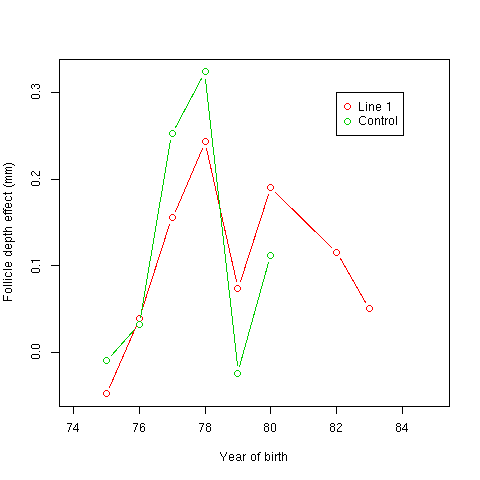
\includegraphics[width=0.9\textwidth]{dgl1.png}
%  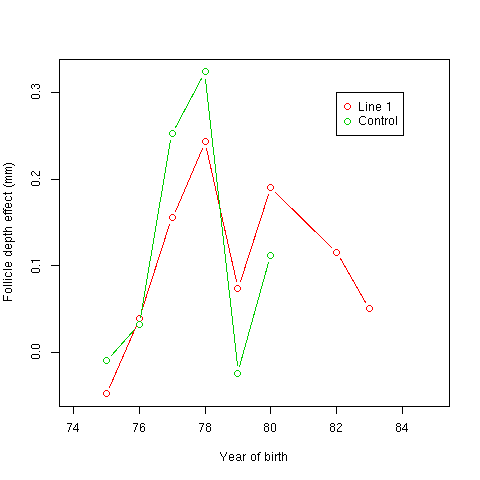
\includegraphics{dgl1.png}
  \caption{Direct response to selection for follicle depth in Line 1. Shifts in the difference between Line 1 and Control Line represent genetic change.}
  \label{fig:dgl1}
\end{figure}

%\end{document}



 Line 1 starts out with a smaller Fd than the Control Line, but changes from 1979 onward to having a larger Fd than the Control Line. There are a lot of data points missing. I am still waiting for CSIRO to complete the Fd measurements on Line 1 in 1984-85 and on the Control Line in 1981-85. Nevertheless we can conclude that there has been genetic change in Fd in Line 1 due to selection for Fd.

Figure~\ref{fig:dgl2} shows the direct response plot for Line 2 and the Control Line.

%\documentclass{article}
%\usepackage{graphicx,subfigure}
%\begin{document}

\begin{figure}[!htp]
  \centering
   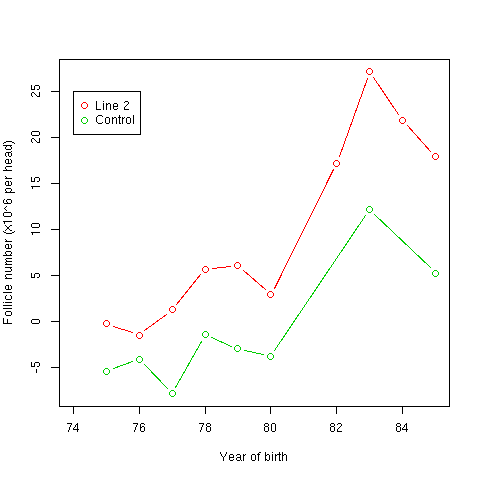
\includegraphics[width=0.9\textwidth]{dgl2.png}
%  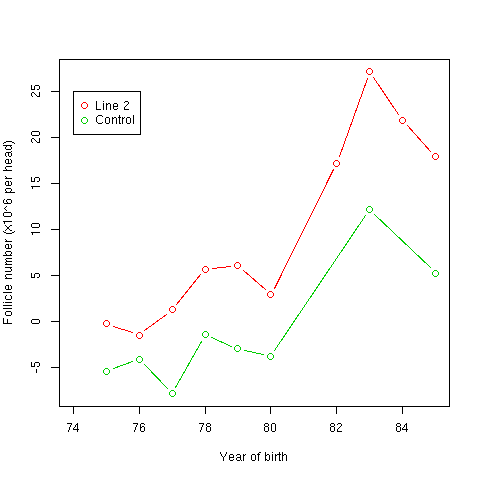
\includegraphics{dgl2.png}
  \caption{Direct response to selection for follicle number per head in Line 2. Shifts in the difference between Line 2 and Control Line represent genetic change.}
  \label{fig:dgl2}
\end{figure}

%\end{document}


Line 2 starts out with a larger number of follicles than the Control Line, and this difference increases with time. We can conclude that there has been genetic change in Fnt in Line 2 due to selection for Fnt. There is also a considerable environmental shift between years 80 and 82, both Line 2 and the Control Line have increased follicle numnber and this jump is manintained thereafter. The cause of this jump is unknown. It may be significant that there was a change of techniwue from manual counting to semi-automatic image processing in 1982.

Figure~\ref{fig:dgl3fd} shows the direct response plot for follicle depth for Line 3 and the Control Line. Figure~\ref{fig:dgl3fnt} shows the direct response plot for follicle number per head for Line 3 and the Control Line.

%\documentclass{article}
%\usepackage{graphicx,subfigure}
%\begin{document}

\begin{figure}[!htp]
  \centering
   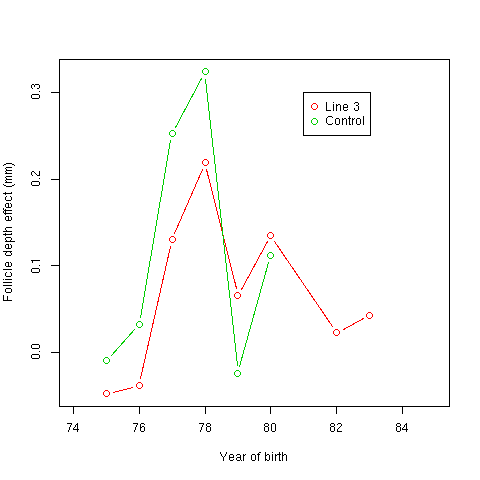
\includegraphics[width=0.9\textwidth]{dgl3fd.png}
%  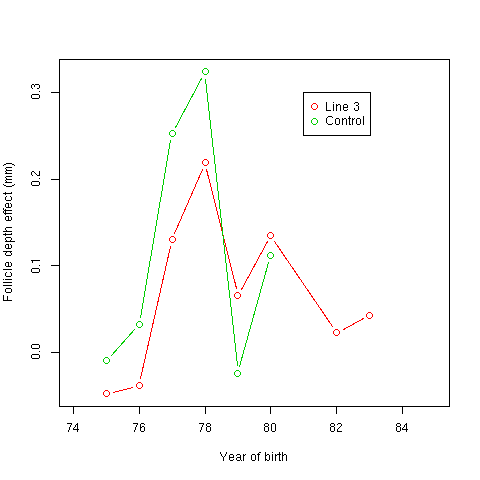
\includegraphics{dgl3fd.png}
  \caption{Direct response in follicle depth, to selection for follicle depth and follicle number per head in Line 3. Shifts in the difference between Line 3 and Control Line represent genetic change.}
  \label{fig:dgl3fd}
\end{figure}

%\end{document}


%\documentclass{article}
%\usepackage{graphicx,subfigure}
%\begin{document}

\begin{figure}[!htp]
  \centering
   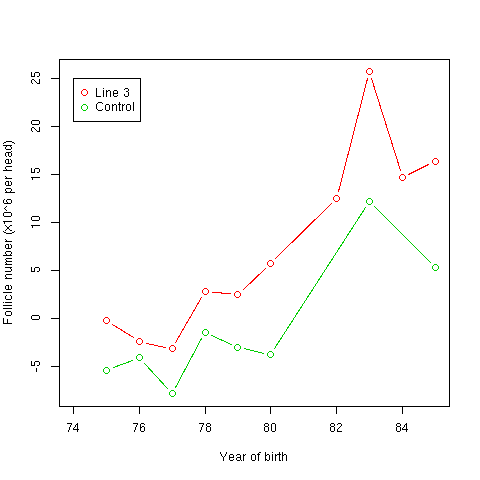
\includegraphics[width=0.9\textwidth]{dgl3fnt.png}
%  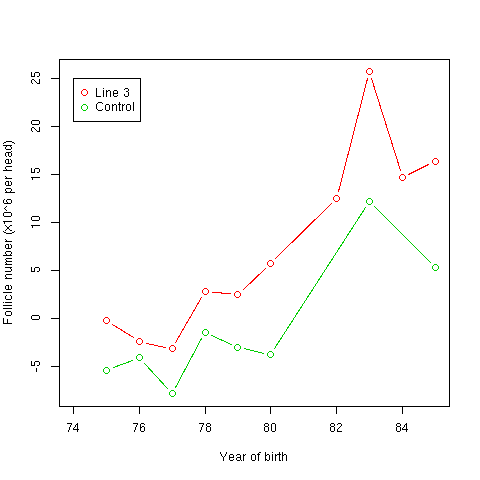
\includegraphics{dgl3fnt.png}
  \caption{Direct response in follicle number per head, to selection for follicle depth and follicle number per head in Line 3. Shifts in the difference between Line 3 and Control Line represent genetic change.}
  \label{fig:dgl3fnt}
\end{figure}

%\end{document}



Line 3 has achieved genetic change in both follicle depth and follicle number per head. The shift in follicle number between years 80 and 82 is again present. 

\subsection{Indirect responses to selection}
We will just look at indirect responses in clean wool weight, fibre diameter and staple length.

Figure~\ref{fig:dgcww} shows the indirect or correlated changes in clean wool weight ({\em Cwwadj}) in all three lines. There is no obvious change in clean wool weight in any of the three lines. There is a slight suggestion that the selected line might average out above the control line in both Line 2 and Line 3. This is not what was expected. The original thinking behind this experiment was that if one wanted to engineer a change in wool weight one had to put selection pressure on all of its components. The components of wool weight in this scenario were considred to be follicle size ( measured as follicle depth) and number of follicles ( measured as follicle number per head). It was expected that there would be a change in wool weight in Line 3 only. This did not occur. Possible explanations are
\begin{itemize}
\item the experiment did not continue for long enough
\item the two components ( follicle size and number) are in some way not an adequate representation of the biology of wool growth
\item the concept of components is somehow flawed
\end{itemize}

%\documentclass{article}
%\usepackage{graphicx,subfigure}
%\begin{document}

\begin{figure}[!htp]
  \centering
   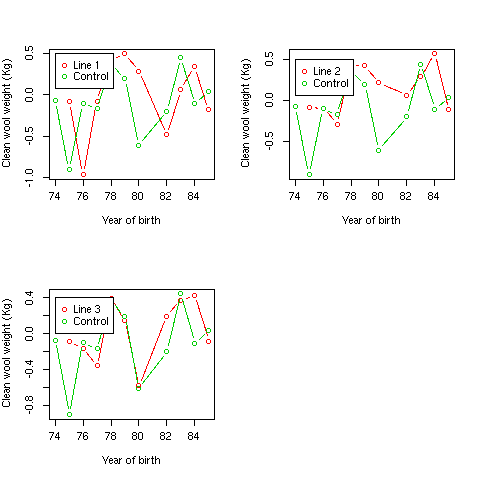
\includegraphics[width=0.9\textwidth]{dgcww.png}
%  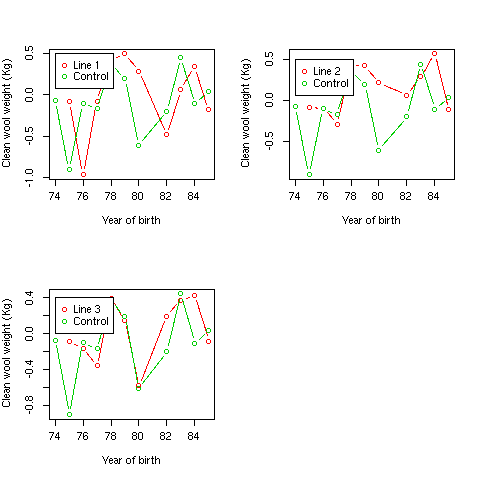
\includegraphics{dgcww.png}
  \caption{Indirect response in clean wool weight, to selection for follicle depth in Line 1, follicle number per head in Line 2, and follicle depth and follicle number per head in Line 3. Shifts in the difference between  each Line and the  Control Line represent genetic change.}
  \label{fig:dgcww}
\end{figure}

%\end{document}


We can look into this a little more thoroughly by seeing if there were any correlated changes in fibre diameter or in fibre length growth rate ( measured as staple length).

Figure~\ref{fig:dgdiam} and Figure~\ref{fig:dgstal} show the correlated changes in average fibre diameter and staple length.

%\documentclass{article}
%\usepackage{graphicx,subfigure}
%\begin{document}

\begin{figure}[!htp]
  \centering
   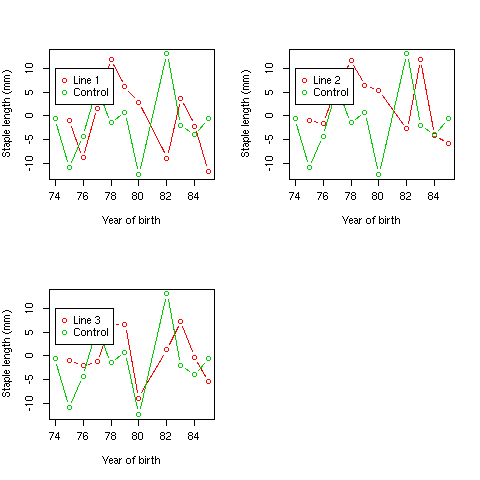
\includegraphics[width=0.9\textwidth]{dgstal.png}
%  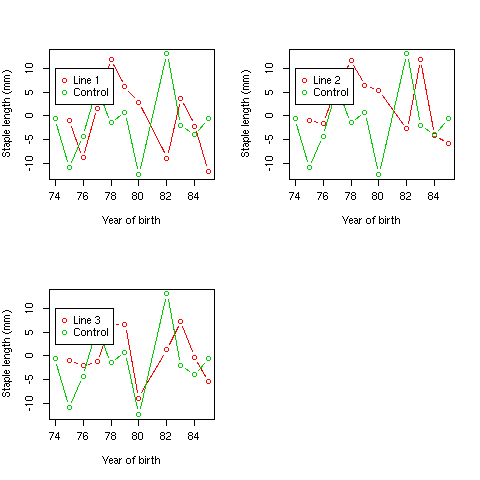
\includegraphics{dgstal.png}
  \caption{Indirect response in staple length, to selection for follicle depth in Line 1, follicle number per head in Line 2, and follicle depth and follicle number per head in Line 3. Shifts in the difference between  each Line and the  Control Line represent genetic change.}
  \label{fig:dgstal}
\end{figure}

%\end{document}


%\documentclass{article}
%\usepackage{graphicx,subfigure}
%\begin{document}

\begin{figure}[!htp]
  \centering
   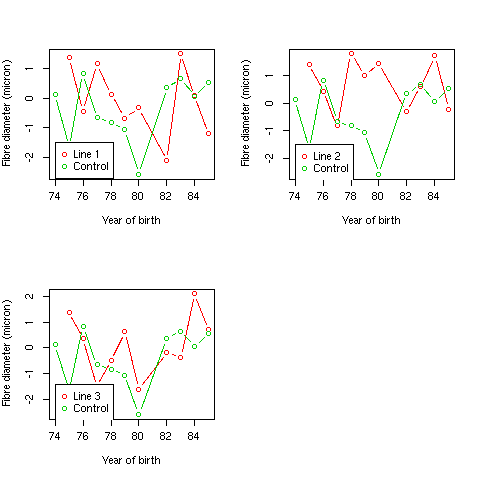
\includegraphics[width=0.9\textwidth]{dgdiam.png}
%  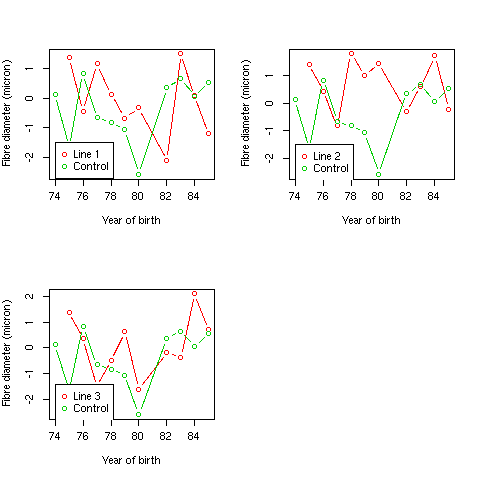
\includegraphics{dgdiam.png}
  \caption{Indirect response in fibre diameter, to selection for follicle depth in Line 1, follicle number per head in Line 2, and follicle depth and follicle number per head in Line 3. Shifts in the difference between  each Line and the  Control Line represent genetic change.}
  \label{fig:dgdiam}
\end{figure}

%\end{document}


There are no obvious correlated changes in staple length or fibre diameter in any of the 3 lines. There is a slight suggestion that staple length might average out higher than the Control line in Lines 2 and 3, as was observeed for clean wool weight. It is becoming clear that the experiment simply did not continue for enough years for correlated responses to be studied. Correlated genetic change is almost always smaller than direct responses to selection, and will therefore take more generations to detect. 

In view of the above, the experiment was simply not carried on for long enough to fulfil its original aim. The hypothesis that one can 'engineer' a genetic improvement in wool weight by changing its components in a coordinated way, is still open. A more detailed analysis of responses against amount of selection applied, is not warranted, and would be difficult to carry out because of the missing observations.

The experiment does however provide an important pedigreed data set with some interesting measurements not available elsewhere. We now proceed to an analysis of the pedigree data.

\clearpage
\subsection{Parameters}
It is important to present phenotypic as well as genetic parameters. They are required in calculating responses to selection. Heritabilities and genetic correlations alone are not suffficient.

\subsubsection{Phenotypic variances}
Phenotypic variances and their standard errors are presented in Table~\ref{tab:pvar}
%\documentclass{article}
%\usepackage{lscape,longtable}
%\begin{document}
% latex table generated in R 3.4.2 by xtable 1.8-2 package
% Tue Oct 17 21:07:46 2017

\begin{center}
\begin{longtable}{|p{1.5in}|p{0.8in}|p{0.8in}|p{0.8in}|p{0.8in}|}
\caption{Estimates of phenotypic variance with standard errors and confidence limits for 56 skin and wool traits} \\
\hline
\label{tab:pvar}
  Traitpair & Estimate & StdErr & CI95lo & CI95hi \\ 
  \hline
\endfirsthead
\multicolumn{5}{c}%
{\tablename\ \thetable\ -- \textit{Continued from previous page}} \\
\hline
    Traitpair & Estimate  & StdErr & CI95lo  &  CI95hi \\
\hline
\endhead
\hline
\multicolumn{5}{r}{\textit{Continued on next page}} \\
\endfoot
\hline
\endlastfoot

 Stal:Stal & 87.501 & 1.423 & 84.711 & 90.290 \\ 
 Diam:Diam & 1.998 & 0.032 & 1.934 & 2.061 \\ 
 Bwt:Bwt & 18.238 & 0.297 & 17.657 & 18.820 \\ 
 WrN:WrN & 0.575 & 0.009 & 0.557 & 0.594 \\ 
 WrB:WrB & 0.614 & 0.010 & 0.595 & 0.634 \\ 
 WrT:WrT & 2.017 & 0.033 & 1.953 & 2.081 \\ 
 Face:Face & 1.113 & 0.018 & 1.078 & 1.147 \\ 
 Gfw:Gfw & 0.249 & 0.004 & 0.241 & 0.257 \\ 
 Yld:Yld & 22.216 & 0.358 & 21.514 & 22.919 \\ 
 Cww:Cww & 0.120 & 0.002 & 0.116 & 0.124 \\ 
 Staladj:Staladj & 126.588 & 2.075 & 122.520 & 130.656 \\ 
 Gfwadj:Gfwadj & 0.357 & 0.006 & 0.346 & 0.369 \\ 
 Cwwadj:Cwwadj & 0.168 & 0.003 & 0.163 & 0.174 \\ 
 Crimp:Crimp & 5.361 & 0.106 & 5.154 & 5.569 \\ 
 Crwvl:Crwvl & 0.225 & 0.004 & 0.216 & 0.233 \\ 
 Crst:Crst & 56.780 & 1.183 & 54.461 & 59.099 \\ 
 Crstadj:Crstadj & 81.204 & 1.696 & 77.880 & 84.528 \\ 
 Crwvt:Crwvt & 0.031 & 0.001 & 0.029 & 0.032 \\ 
 Dp:Dp & 11.806 & 0.389 & 11.042 & 12.569 \\ 
 Ds:Ds & 4.059 & 0.135 & 3.794 & 4.324 \\ 
 Dps:Dps & 3.987 & 0.133 & 3.727 & 4.248 \\ 
 DpovDs:DpovDs & 0.028 & 0.001 & 0.026 & 0.029 \\ 
 CVDp:CVDp & 20.746 & 0.697 & 19.381 & 22.111 \\ 
 CVDs:CVDs & 7.378 & 0.249 & 6.891 & 7.866 \\ 
 MaxDp:MaxDp & 44.886 & 1.489 & 41.966 & 47.805 \\ 
 MinDp:MinDp & 12.649 & 0.434 & 11.799 & 13.500 \\ 
 MaxDs:MaxDs & 26.440 & 0.893 & 24.689 & 28.191 \\ 
 MinDs:MinDs & 5.890 & 0.200 & 5.499 & 6.281 \\ 
 SDDp:SDDp & 1.954 & 0.064 & 1.828 & 2.080 \\ 
 SDDs:SDDs & 0.335 & 0.011 & 0.313 & 0.357 \\ 
 SDD:SDD & 0.340 & 0.011 & 0.318 & 0.362 \\ 
 CVD:CVD & 7.128 & 0.240 & 6.658 & 7.598 \\ 
 Gt30Dp:Gt30Dp & 278.347 & 9.248 & 260.221 & 296.473 \\ 
 Gt30Ds:Gt30Ds & 7.879 & 0.265 & 7.359 & 8.399 \\ 
 Gt30D:Gt30D & 9.396 & 0.316 & 8.776 & 10.015 \\ 
 Fnua:Fnua & 148.641 & 2.625 & 143.495 & 153.786 \\ 
 Fr:Fr & 15.004 & 0.265 & 14.485 & 15.523 \\ 
 Fnt:Fnt & 143.441 & 2.532 & 138.478 & 148.403 \\ 
 Sarea:Sarea & 0.007 & 0.000 & 0.006 & 0.007 \\ 
 Fd:Fd & 0.023 & 0.000 & 0.022 & 0.024 \\ 
 Fc:Fc & 1.240 & 0.024 & 1.194 & 1.287 \\ 
 Fu:Fu & 0.645 & 0.012 & 0.620 & 0.669 \\ 
 Colour:Colour & 0.599 & 0.010 & 0.580 & 0.619 \\ 
 Fly:Fly & 1.849 & 0.031 & 1.788 & 1.911 \\ 
 Flcrot:Flcrot & 3.066 & 0.052 & 2.964 & 3.168 \\ 
 Bactst:Bactst & 0.117 & 0.002 & 0.112 & 0.122 \\ 
 MycD:MycD & 0.544 & 0.011 & 0.522 & 0.567 \\ 
 Bcts:Bcts & 2.096 & 0.036 & 2.026 & 2.165 \\ 
 Bctb:Bctb & 2.274 & 0.039 & 2.199 & 2.350 \\ 
 Weanwt:Weanwt & 8.804 & 0.154 & 8.502 & 9.105 \\ 
 NLB:NLB & 0.209 & 0.003 & 0.202 & 0.216 \\ 
 NLW:NLW & 0.173 & 0.003 & 0.168 & 0.179 \\ 
 Fnpua:Fnpua & 0.395 & 0.007 & 0.381 & 0.408 \\ 
 Fnsua:Fnsua & 142.081 & 2.509 & 137.163 & 146.999 \\ 
 Fnpt:Fnpt & 0.385 & 0.007 & 0.372 & 0.398 \\ 
 Fnst:Fnst & 137.073 & 2.420 & 132.331 & 141.816 \\ 
 \hline
\end{longtable}
\end{center}
%\end{document}


The columns CI95lo and CI95hi represent the lower and upper limits of a 95 per
cent confidence interval for the variance estimate.

\subsubsection{Correlations}
Phenotypic, genetic and environmental correlations for each pair of traits are presented in Table~\ref{tab:corr}
%\documentclass{article}
%\usepackage{lscape,longtable}
%\begin{document}
% latex table generated in R 3.4.2 by xtable 1.8-2 package
% Fri Oct 20 21:06:30 2017

\begin{center}
\begin{longtable}{|p{1.1in}|p{0.7in}|p{0.7in}|p{0.6in}|p{0.6in}|p{0.6in}|}
\caption{Estimates of individual environmental(E(I)), individual additive genetic(G(Ia)), and phenotypic(P(I)) correlations with standard errors and confidence limits for 56 skin and wool traits} \\
\hline
\label{tab:corr}
  Traitpair & Component & Estimate & StdErr & CI95lo & CI95hi \\
  \hline
\endfirsthead
\multicolumn{5}{c}%
{\tablename\ \thetable\ -- \textit{Continued from previous page}} \\
\hline
    Traitpair & Component & Estimate  & StdErr & CI95lo  &  CI95hi \\
\hline
\endhead
\hline
\multicolumn{5}{r}{\textit{Continued on next page}} \\
\endfoot
\hline
\endlastfoot

  Stal:Stal & E(I) & 1.00 & 0.00 & 1.00 & 1.00 \\ 
  Stal:Stal & G(Ia) & 1.00 & 0.00 & 1.00 & 1.00 \\ 
  Stal:Stal & P(I) & 1.00 & 0.00 & 1.00 & 1.00 \\ 
  Stal:Diam & E(I) & 0.12 & 0.03 & 0.06 & 0.19 \\ 
  Stal:Diam & G(Ia) & 0.14 & 0.03 & 0.09 & 0.20 \\ 
  Stal:Diam & P(I) & 0.13 & 0.02 & 0.10 & 0.16 \\ 
  Stal:Bwt & E(I) & 0.26 & 0.03 & 0.20 & 0.31 \\ 
  Stal:Bwt & G(Ia) & 0.08 & 0.03 & 0.02 & 0.14 \\ 
  Stal:Bwt & P(I) & 0.19 & 0.02 & 0.16 & 0.23 \\ 
  Stal:WrN & E(I) & -0.12 & 0.03 & -0.18 & -0.06 \\ 
  Stal:WrN & G(Ia) & -0.21 & 0.03 & -0.27 & -0.15 \\ 
  Stal:WrN & P(I) & -0.15 & 0.02 & -0.18 & -0.12 \\ 
  Stal:WrB & E(I) & -0.09 & 0.03 & -0.15 & -0.03 \\ 
  Stal:WrB & G(Ia) & -0.24 & 0.03 & -0.30 & -0.19 \\ 
  Stal:WrB & P(I) & -0.15 & 0.02 & -0.18 & -0.11 \\ 
  Stal:WrT & E(I) & -0.11 & 0.03 & -0.17 & -0.05 \\ 
  Stal:WrT & G(Ia) & -0.22 & 0.03 & -0.28 & -0.17 \\ 
  Stal:WrT & P(I) & -0.16 & 0.02 & -0.19 & -0.12 \\ 
  Stal:Face & E(I) & -0.02 & 0.04 & -0.10 & 0.07 \\ 
  Stal:Face & G(Ia) & -0.31 & 0.02 & -0.35 & -0.27 \\ 
  Stal:Face & P(I) & -0.16 & 0.02 & -0.19 & -0.13 \\ 
  Stal:Gfw & E(I) & 0.17 & 0.03 & 0.11 & 0.23 \\ 
  Stal:Gfw & G(Ia) & 0.53 & 0.03 & 0.47 & 0.58 \\ 
  Stal:Gfw & P(I) & 0.30 & 0.02 & 0.27 & 0.33 \\ 
  Stal:Yld & E(I) & 0.36 & 0.03 & 0.30 & 0.42 \\ 
  Stal:Yld & G(Ia) & 0.11 & 0.03 & 0.06 & 0.17 \\ 
  Stal:Yld & P(I) & 0.26 & 0.02 & 0.23 & 0.29 \\ 
  Stal:Cww & E(I) & 0.31 & 0.03 & 0.25 & 0.36 \\ 
  Stal:Cww & G(Ia) & 0.59 & 0.03 & 0.54 & 0.64 \\ 
  Stal:Cww & P(I) & 0.41 & 0.01 & 0.38 & 0.43 \\ 
  Stal:Staladj & E(I) & 0.97 & 0.00 & 0.96 & 0.98 \\ 
  Stal:Staladj & G(Ia) & 0.99 & 0.00 & 0.99 & 1.00 \\ 
  Stal:Staladj & P(I) & 0.98 & 0.00 & 0.97 & 0.98 \\ 
  Stal:Gfwadj & E(I) & 0.14 & 0.03 & 0.09 & 0.20 \\ 
  Stal:Gfwadj & G(Ia) & 0.51 & 0.03 & 0.45 & 0.56 \\ 
  Stal:Gfwadj & P(I) & 0.27 & 0.02 & 0.24 & 0.30 \\ 
  Stal:Cwwadj & E(I) & 0.28 & 0.03 & 0.23 & 0.33 \\ 
  Stal:Cwwadj & G(Ia) & 0.58 & 0.03 & 0.52 & 0.63 \\ 
  Stal:Cwwadj & P(I) & 0.38 & 0.01 & 0.35 & 0.41 \\ 
  Stal:Crimp & E(I) & 0.41 & 0.21 & -0.00 & 0.82 \\ 
  Stal:Crimp & G(Ia) & -0.58 & 0.03 & -0.63 & -0.53 \\ 
  Stal:Crimp & P(I) & -0.28 & 0.02 & -0.32 & -0.24 \\ 
  Stal:Crwvl & E(I) & -0.06 & 0.04 & -0.14 & 0.03 \\ 
  Stal:Crwvl & G(Ia) & 0.55 & 0.03 & 0.48 & 0.61 \\ 
  Stal:Crwvl & P(I) & 0.21 & 0.02 & 0.17 & 0.24 \\ 
  Stal:Crst & E(I) & 0.95 & 0.06 & 0.84 & 1.07 \\ 
  Stal:Crst & G(Ia) & -0.22 & 0.04 & -0.29 & -0.15 \\ 
  Stal:Crst & P(I) & 0.31 & 0.02 & 0.28 & 0.35 \\ 
  Stal:Crstadj & E(I) & 0.89 & 0.05 & 0.78 & 0.99 \\ 
  Stal:Crstadj & G(Ia) & -0.21 & 0.04 & -0.28 & -0.14 \\ 
  Stal:Crstadj & P(I) & 0.31 & 0.02 & 0.27 & 0.35 \\ 
  Stal:Crwvt & E(I) & -0.66 & 0.04 & -0.74 & -0.58 \\ 
  Stal:Crwvt & G(Ia) & 0.16 & 0.04 & 0.08 & 0.24 \\ 
  Stal:Crwvt & P(I) & -0.30 & 0.02 & -0.34 & -0.27 \\ 
  Stal:Dp & E(I) & 0.09 & 0.09 & -0.08 & 0.26 \\ 
  Stal:Dp & G(Ia) & -0.19 & 0.05 & -0.30 & -0.08 \\ 
  Stal:Dp & P(I) & -0.05 & 0.03 & -0.12 & 0.01 \\ 
  Stal:Ds & E(I) & -0.06 & 0.08 & -0.21 & 0.09 \\ 
  Stal:Ds & G(Ia) & 0.36 & 0.06 & 0.24 & 0.49 \\ 
  Stal:Ds & P(I) & 0.13 & 0.03 & 0.06 & 0.19 \\ 
  Stal:Dps & E(I) & -0.05 & 0.08 & -0.20 & 0.09 \\ 
  Stal:Dps & G(Ia) & 0.35 & 0.06 & 0.23 & 0.48 \\ 
  Stal:Dps & P(I) & 0.12 & 0.03 & 0.06 & 0.19 \\ 
  Stal:DpovDs & E(I) & 0.19 & 0.14 & -0.08 & 0.46 \\ 
  Stal:DpovDs & G(Ia) & -0.34 & 0.04 & -0.42 & -0.25 \\ 
  Stal:DpovDs & P(I) & -0.15 & 0.03 & -0.21 & -0.09 \\ 
  Stal:CVDp & E(I) & -0.15 & 0.07 & -0.29 & -0.01 \\ 
  Stal:CVDp & G(Ia) & 0.05 & 0.07 & -0.09 & 0.19 \\ 
  Stal:CVDp & P(I) & -0.07 & 0.03 & -0.13 & -0.00 \\ 
  Stal:CVDs & E(I) & -0.17 & 0.07 & -0.31 & -0.04 \\ 
  Stal:CVDs & G(Ia) & -0.09 & 0.08 & -0.23 & 0.06 \\ 
  Stal:CVDs & P(I) & -0.14 & 0.03 & -0.20 & -0.07 \\ 
  Stal:MaxDp & E(I) & 0.07 & 0.08 & -0.09 & 0.24 \\ 
  Stal:MaxDp & G(Ia) & -0.17 & 0.06 & -0.28 & -0.06 \\ 
  Stal:MaxDp & P(I) & -0.05 & 0.03 & -0.11 & 0.02 \\ 
  Stal:MinDp & E(I) & 0.22 & 0.06 & 0.09 & 0.34 \\ 
  Stal:MinDp & G(Ia) & -0.74 & 0.18 & -1.09 & -0.39 \\ 
  Stal:MinDp & P(I) & -0.01 & 0.03 & -0.07 & 0.06 \\ 
  Stal:MaxDs & E(I) & -0.21 & 0.07 & -0.34 & -0.09 \\ 
  Stal:MaxDs & G(Ia) & 0.20 & 0.09 & 0.01 & 0.39 \\ 
  Stal:MaxDs & P(I) & -0.08 & 0.03 & -0.14 & -0.01 \\ 
  Stal:MinDs & E(I) & -0.02 & 0.06 & -0.14 & 0.10 \\ 
  Stal:MinDs & G(Ia) & 0.20 & 0.16 & -0.12 & 0.52 \\ 
  Stal:MinDs & P(I) & 0.02 & 0.03 & -0.04 & 0.09 \\ 
  Stal:SDDp & E(I) & -0.04 & 0.08 & -0.20 & 0.12 \\ 
  Stal:SDDp & G(Ia) & -0.12 & 0.06 & -0.23 & -0.01 \\ 
  Stal:SDDp & P(I) & -0.08 & 0.03 & -0.14 & -0.02 \\ 
  Stal:SDDs & E(I) & -0.19 & 0.08 & -0.34 & -0.04 \\ 
  Stal:SDDs & G(Ia) & 0.10 & 0.06 & -0.02 & 0.23 \\ 
  Stal:SDDs & P(I) & -0.06 & 0.03 & -0.12 & 0.01 \\ 
  Stal:SDD & E(I) & -0.18 & 0.08 & -0.33 & -0.03 \\ 
  Stal:SDD & G(Ia) & 0.08 & 0.06 & -0.05 & 0.20 \\ 
  Stal:SDD & P(I) & -0.06 & 0.03 & -0.13 & 0.00 \\ 
  Stal:CVD & E(I) & -0.17 & 0.07 & -0.30 & -0.03 \\ 
  Stal:CVD & G(Ia) & -0.11 & 0.07 & -0.25 & 0.04 \\ 
  Stal:CVD & P(I) & -0.14 & 0.03 & -0.21 & -0.08 \\ 
  Stal:Gt30Dp & E(I) & 0.07 & 0.08 & -0.09 & 0.23 \\ 
  Stal:Gt30Dp & G(Ia) & -0.21 & 0.06 & -0.33 & -0.10 \\ 
  Stal:Gt30Dp & P(I) & -0.07 & 0.03 & -0.13 & -0.00 \\ 
  Stal:Gt30Ds & E(I) & -0.06 & 0.07 & -0.19 & 0.08 \\ 
  Stal:Gt30Ds & G(Ia) & 0.10 & 0.08 & -0.05 & 0.25 \\ 
  Stal:Gt30Ds & P(I) & 0.00 & 0.03 & -0.06 & 0.07 \\ 
  Stal:Gt30D & E(I) & -0.04 & 0.07 & -0.18 & 0.10 \\ 
  Stal:Gt30D & G(Ia) & 0.05 & 0.07 & -0.10 & 0.19 \\ 
  Stal:Gt30D & P(I) & -0.01 & 0.03 & -0.07 & 0.06 \\ 
  Stal:Fnua & E(I) & -0.19 & 0.03 & -0.25 & -0.13 \\ 
  Stal:Fnua & G(Ia) & -0.13 & 0.04 & -0.20 & -0.06 \\ 
  Stal:Fnua & P(I) & -0.17 & 0.02 & -0.20 & -0.14 \\ 
  Stal:Fr & E(I) & -0.07 & 0.03 & -0.13 & -0.01 \\ 
  Stal:Fr & G(Ia) & -0.25 & 0.04 & -0.32 & -0.18 \\ 
  Stal:Fr & P(I) & -0.13 & 0.02 & -0.17 & -0.10 \\ 
  Stal:Fnt & E(I) & -0.07 & 0.03 & -0.13 & -0.01 \\ 
  Stal:Fnt & G(Ia) & -0.06 & 0.04 & -0.14 & 0.01 \\ 
  Stal:Fnt & P(I) & -0.07 & 0.02 & -0.11 & -0.04 \\ 
  Stal:Sarea & E(I) & 0.26 & 0.03 & 0.20 & 0.32 \\ 
  Stal:Sarea & G(Ia) & 0.10 & 0.03 & 0.04 & 0.17 \\ 
  Stal:Sarea & P(I) & 0.20 & 0.02 & 0.17 & 0.24 \\ 
  Stal:Fd & E(I) & 0.16 & 0.03 & 0.10 & 0.22 \\ 
  Stal:Fd & G(Ia) & 0.42 & 0.05 & 0.32 & 0.53 \\ 
  Stal:Fd & P(I) & 0.22 & 0.02 & 0.18 & 0.26 \\ 
  Stal:Fc & E(I) & 0.03 & 0.05 & -0.06 & 0.13 \\ 
  Stal:Fc & G(Ia) & -0.44 & 0.03 & -0.50 & -0.38 \\ 
  Stal:Fc & P(I) & -0.19 & 0.02 & -0.22 & -0.15 \\ 
  Stal:Fu & E(I) & -0.06 & 0.04 & -0.13 & 0.01 \\ 
  Stal:Fu & G(Ia) & -0.36 & 0.04 & -0.44 & -0.29 \\ 
  Stal:Fu & P(I) & -0.17 & 0.02 & -0.20 & -0.13 \\ 
  Stal:Colour & E(I) & -0.10 & 0.03 & -0.16 & -0.05 \\ 
  Stal:Colour & G(Ia) & 0.02 & 0.05 & -0.07 & 0.11 \\ 
  Stal:Colour & P(I) & -0.07 & 0.02 & -0.10 & -0.04 \\ 
  Stal:Fly & E(I) & 0.13 & 0.03 & 0.08 & 0.18 \\ 
  Stal:Fly & G(Ia) & -0.52 & 0.07 & -0.66 & -0.38 \\ 
  Stal:Fly & P(I) & -0.00 & 0.02 & -0.03 & 0.03 \\ 
  Stal:Flcrot & E(I) & -0.01 & 0.03 & -0.06 & 0.04 \\ 
  Stal:Flcrot & G(Ia) & -0.10 & 0.11 & -0.32 & 0.11 \\ 
  Stal:Flcrot & P(I) & -0.02 & 0.02 & -0.05 & 0.01 \\ 
  Stal:Bactst & E(I) & -0.05 & 0.03 & -0.11 & 0.02 \\ 
  Stal:Bactst & G(Ia) & -0.55 & 0.14 & -0.82 & -0.29 \\ 
  Stal:Bactst & P(I) & -0.11 & 0.02 & -0.15 & -0.07 \\ 
  Stal:MycD & E(I) & 0.01 & 0.03 & -0.05 & 0.08 \\ 
  Stal:MycD & G(Ia) & -0.27 & 0.12 & -0.51 & -0.03 \\ 
  Stal:MycD & P(I) & -0.03 & 0.02 & -0.07 & 0.01 \\ 
  Stal:Bcts & E(I) & 0.33 & 0.06 & 0.21 & 0.45 \\ 
  Stal:Bcts & G(Ia) & -0.16 & 0.02 & -0.20 & -0.11 \\ 
  Stal:Bcts & P(I) & 0.03 & 0.02 & -0.00 & 0.07 \\ 
  Stal:Bctb & E(I) & 0.32 & 0.06 & 0.21 & 0.43 \\ 
  Stal:Bctb & G(Ia) & -0.19 & 0.02 & -0.24 & -0.14 \\ 
  Stal:Bctb & P(I) & 0.02 & 0.02 & -0.01 & 0.06 \\ 
  Stal:Weanwt & E(I) & 0.11 & 0.03 & 0.05 & 0.17 \\ 
  Stal:Weanwt & G(Ia) & -0.02 & 0.04 & -0.11 & 0.06 \\ 
  Stal:Weanwt & P(I) & 0.07 & 0.02 & 0.04 & 0.10 \\ 
  Stal:NLB & E(I) & -0.04 & 0.03 & -0.10 & 0.01 \\ 
  Stal:NLB & G(Ia) & 0.27 & 0.04 & 0.19 & 0.36 \\ 
  Stal:NLB & P(I) & 0.04 & 0.02 & 0.01 & 0.07 \\ 
  Stal:NLW & E(I) & 0.03 & 0.03 & -0.03 & 0.08 \\ 
  Stal:NLW & G(Ia) & 0.14 & 0.04 & 0.06 & 0.22 \\ 
  Stal:NLW & P(I) & 0.06 & 0.02 & 0.03 & 0.09 \\ 
  Stal:Fnpua & E(I) & -0.11 & 0.03 & -0.16 & -0.05 \\ 
  Stal:Fnpua & G(Ia) & 0.12 & 0.04 & 0.03 & 0.20 \\ 
  Stal:Fnpua & P(I) & -0.04 & 0.02 & -0.08 & -0.01 \\ 
  Stal:Fnsua & E(I) & -0.19 & 0.03 & -0.25 & -0.13 \\ 
  Stal:Fnsua & G(Ia) & -0.14 & 0.04 & -0.21 & -0.06 \\ 
  Stal:Fnsua & P(I) & -0.17 & 0.02 & -0.21 & -0.14 \\ 
  Stal:Fnpt & E(I) & 0.00 & 0.03 & -0.06 & 0.06 \\ 
  Stal:Fnpt & G(Ia) & 0.16 & 0.04 & 0.08 & 0.24 \\ 
  Stal:Fnpt & P(I) & 0.05 & 0.02 & 0.01 & 0.08 \\ 
  Stal:Fnst & E(I) & -0.08 & 0.03 & -0.14 & -0.01 \\ 
  Stal:Fnst & G(Ia) & -0.07 & 0.04 & -0.15 & -0.00 \\ 
  Stal:Fnst & P(I) & -0.08 & 0.02 & -0.11 & -0.04 \\ 
  Diam:Stal & E(I) & 0.12 & 0.03 & 0.06 & 0.19 \\ 
  Diam:Stal & G(Ia) & 0.14 & 0.03 & 0.09 & 0.20 \\ 
  Diam:Stal & P(I) & 0.13 & 0.02 & 0.10 & 0.16 \\ 
  Diam:Diam & E(I) & 1.00 & 0.00 & 1.00 & 1.00 \\ 
  Diam:Diam & G(Ia) & 1.00 & 0.00 & 1.00 & 1.00 \\ 
  Diam:Diam & P(I) & 1.00 & 0.00 & 1.00 & 1.00 \\ 
  Diam:Bwt & E(I) & 0.20 & 0.03 & 0.14 & 0.26 \\ 
  Diam:Bwt & G(Ia) & 0.15 & 0.03 & 0.10 & 0.20 \\ 
  Diam:Bwt & P(I) & 0.18 & 0.02 & 0.15 & 0.21 \\ 
  Diam:WrN & E(I) & 0.17 & 0.03 & 0.11 & 0.24 \\ 
  Diam:WrN & G(Ia) & 0.22 & 0.03 & 0.17 & 0.27 \\ 
  Diam:WrN & P(I) & 0.19 & 0.02 & 0.16 & 0.23 \\ 
  Diam:WrB & E(I) & 0.20 & 0.03 & 0.13 & 0.26 \\ 
  Diam:WrB & G(Ia) & 0.15 & 0.03 & 0.10 & 0.20 \\ 
  Diam:WrB & P(I) & 0.18 & 0.02 & 0.15 & 0.21 \\ 
  Diam:WrT & E(I) & 0.21 & 0.03 & 0.15 & 0.28 \\ 
  Diam:WrT & G(Ia) & 0.19 & 0.02 & 0.15 & 0.24 \\ 
  Diam:WrT & P(I) & 0.20 & 0.02 & 0.17 & 0.23 \\ 
  Diam:Face & E(I) & -0.03 & 0.05 & -0.12 & 0.07 \\ 
  Diam:Face & G(Ia) & -0.12 & 0.02 & -0.16 & -0.08 \\ 
  Diam:Face & P(I) & -0.08 & 0.02 & -0.11 & -0.05 \\ 
  Diam:Gfw & E(I) & 0.29 & 0.03 & 0.23 & 0.35 \\ 
  Diam:Gfw & G(Ia) & 0.56 & 0.02 & 0.51 & 0.60 \\ 
  Diam:Gfw & P(I) & 0.39 & 0.01 & 0.37 & 0.42 \\ 
  Diam:Yld & E(I) & -0.05 & 0.04 & -0.12 & 0.02 \\ 
  Diam:Yld & G(Ia) & -0.17 & 0.02 & -0.22 & -0.12 \\ 
  Diam:Yld & P(I) & -0.10 & 0.02 & -0.13 & -0.07 \\ 
  Diam:Cww & E(I) & 0.25 & 0.03 & 0.19 & 0.31 \\ 
  Diam:Cww & G(Ia) & 0.48 & 0.03 & 0.43 & 0.53 \\ 
  Diam:Cww & P(I) & 0.34 & 0.01 & 0.31 & 0.37 \\ 
  Diam:Staladj & E(I) & 0.13 & 0.03 & 0.07 & 0.19 \\ 
  Diam:Staladj & G(Ia) & 0.13 & 0.03 & 0.08 & 0.18 \\ 
  Diam:Staladj & P(I) & 0.13 & 0.02 & 0.10 & 0.16 \\ 
  Diam:Gfwadj & E(I) & 0.29 & 0.03 & 0.23 & 0.35 \\ 
  Diam:Gfwadj & G(Ia) & 0.55 & 0.02 & 0.50 & 0.60 \\ 
  Diam:Gfwadj & P(I) & 0.39 & 0.01 & 0.36 & 0.42 \\ 
  Diam:Cwwadj & E(I) & 0.26 & 0.03 & 0.20 & 0.31 \\ 
  Diam:Cwwadj & G(Ia) & 0.48 & 0.03 & 0.43 & 0.53 \\ 
  Diam:Cwwadj & P(I) & 0.34 & 0.01 & 0.31 & 0.37 \\ 
  Diam:Crimp & E(I) & 0.33 & 0.18 & -0.03 & 0.68 \\ 
  Diam:Crimp & G(Ia) & -0.44 & 0.03 & -0.49 & -0.38 \\ 
  Diam:Crimp & P(I) & -0.20 & 0.02 & -0.23 & -0.16 \\ 
  Diam:Crwvl & E(I) & -0.17 & 0.04 & -0.25 & -0.09 \\ 
  Diam:Crwvl & G(Ia) & 0.48 & 0.03 & 0.41 & 0.55 \\ 
  Diam:Crwvl & P(I) & 0.10 & 0.02 & 0.07 & 0.14 \\ 
  Diam:Crst & E(I) & 0.18 & 0.06 & 0.06 & 0.29 \\ 
  Diam:Crst & G(Ia) & -0.33 & 0.04 & -0.39 & -0.26 \\ 
  Diam:Crst & P(I) & -0.08 & 0.02 & -0.12 & -0.04 \\ 
  Diam:Crstadj & E(I) & 0.20 & 0.06 & 0.09 & 0.31 \\ 
  Diam:Crstadj & G(Ia) & -0.34 & 0.04 & -0.41 & -0.27 \\ 
  Diam:Crstadj & P(I) & -0.07 & 0.02 & -0.11 & -0.02 \\ 
  Diam:Crwvt & E(I) & -0.16 & 0.05 & -0.25 & -0.07 \\ 
  Diam:Crwvt & G(Ia) & 0.35 & 0.04 & 0.27 & 0.43 \\ 
  Diam:Crwvt & P(I) & 0.05 & 0.02 & 0.01 & 0.09 \\ 
  Diam:Dp & E(I) & 0.63 & 0.08 & 0.48 & 0.78 \\ 
  Diam:Dp & G(Ia) & 0.14 & 0.05 & 0.05 & 0.24 \\ 
  Diam:Dp & P(I) & 0.37 & 0.03 & 0.31 & 0.42 \\ 
  Diam:Ds & E(I) & 0.35 & 0.06 & 0.22 & 0.48 \\ 
  Diam:Ds & G(Ia) & 0.91 & 0.04 & 0.83 & 0.99 \\ 
  Diam:Ds & P(I) & 0.61 & 0.02 & 0.57 & 0.66 \\ 
  Diam:Dps & E(I) & 0.38 & 0.06 & 0.26 & 0.50 \\ 
  Diam:Dps & G(Ia) & 0.93 & 0.04 & 0.85 & 1.01 \\ 
  Diam:Dps & P(I) & 0.63 & 0.02 & 0.58 & 0.67 \\ 
  Diam:DpovDs & E(I) & 0.58 & 0.15 & 0.28 & 0.88 \\ 
  Diam:DpovDs & G(Ia) & -0.33 & 0.04 & -0.41 & -0.24 \\ 
  Diam:DpovDs & P(I) & -0.05 & 0.03 & -0.11 & 0.02 \\ 
  Diam:CVDp & E(I) & -0.07 & 0.08 & -0.22 & 0.09 \\ 
  Diam:CVDp & G(Ia) & 0.30 & 0.06 & 0.18 & 0.43 \\ 
  Diam:CVDp & P(I) & 0.09 & 0.03 & 0.03 & 0.16 \\ 
  Diam:CVDs & E(I) & -0.06 & 0.07 & -0.21 & 0.08 \\ 
  Diam:CVDs & G(Ia) & 0.14 & 0.07 & 0.00 & 0.28 \\ 
  Diam:CVDs & P(I) & 0.02 & 0.03 & -0.04 & 0.09 \\ 
  Diam:MaxDp & E(I) & 0.44 & 0.08 & 0.29 & 0.60 \\ 
  Diam:MaxDp & G(Ia) & 0.16 & 0.05 & 0.07 & 0.26 \\ 
  Diam:MaxDp & P(I) & 0.29 & 0.03 & 0.23 & 0.35 \\ 
  Diam:MinDp & E(I) & 0.26 & 0.06 & 0.14 & 0.39 \\ 
  Diam:MinDp & G(Ia) & 0.03 & 0.11 & -0.19 & 0.24 \\ 
  Diam:MinDp & P(I) & 0.17 & 0.03 & 0.11 & 0.24 \\ 
  Diam:MaxDs & E(I) & 0.20 & 0.06 & 0.08 & 0.33 \\ 
  Diam:MaxDs & G(Ia) & 0.80 & 0.08 & 0.65 & 0.96 \\ 
  Diam:MaxDs & P(I) & 0.39 & 0.03 & 0.33 & 0.44 \\ 
  Diam:MinDs & E(I) & 0.16 & 0.06 & 0.04 & 0.29 \\ 
  Diam:MinDs & G(Ia) & 0.02 & 0.12 & -0.22 & 0.26 \\ 
  Diam:MinDs & P(I) & 0.11 & 0.03 & 0.04 & 0.17 \\ 
  Diam:SDDp & E(I) & 0.25 & 0.08 & 0.09 & 0.41 \\ 
  Diam:SDDp & G(Ia) & 0.22 & 0.05 & 0.12 & 0.32 \\ 
  Diam:SDDp & P(I) & 0.23 & 0.03 & 0.17 & 0.29 \\ 
  Diam:SDDs & E(I) & 0.14 & 0.08 & -0.01 & 0.29 \\ 
  Diam:SDDs & G(Ia) & 0.61 & 0.05 & 0.51 & 0.71 \\ 
  Diam:SDDs & P(I) & 0.36 & 0.03 & 0.30 & 0.42 \\ 
  Diam:SDD & E(I) & 0.17 & 0.08 & 0.03 & 0.32 \\ 
  Diam:SDD & G(Ia) & 0.61 & 0.05 & 0.51 & 0.71 \\ 
  Diam:SDD & P(I) & 0.38 & 0.03 & 0.33 & 0.44 \\ 
  Diam:CVD & E(I) & -0.05 & 0.08 & -0.20 & 0.10 \\ 
  Diam:CVD & G(Ia) & 0.15 & 0.07 & 0.02 & 0.29 \\ 
  Diam:CVD & P(I) & 0.04 & 0.03 & -0.03 & 0.10 \\ 
  Diam:Gt30Dp & E(I) & 0.46 & 0.08 & 0.30 & 0.61 \\ 
  Diam:Gt30Dp & G(Ia) & 0.19 & 0.05 & 0.09 & 0.29 \\ 
  Diam:Gt30Dp & P(I) & 0.32 & 0.03 & 0.26 & 0.38 \\ 
  Diam:Gt30Ds & E(I) & 0.34 & 0.06 & 0.22 & 0.46 \\ 
  Diam:Gt30Ds & G(Ia) & 0.74 & 0.06 & 0.63 & 0.85 \\ 
  Diam:Gt30Ds & P(I) & 0.49 & 0.03 & 0.43 & 0.54 \\ 
  Diam:Gt30D & E(I) & 0.42 & 0.06 & 0.30 & 0.54 \\ 
  Diam:Gt30D & G(Ia) & 0.71 & 0.05 & 0.61 & 0.82 \\ 
  Diam:Gt30D & P(I) & 0.53 & 0.03 & 0.48 & 0.58 \\ 
  Diam:Fnua & E(I) & -0.47 & 0.03 & -0.53 & -0.42 \\ 
  Diam:Fnua & G(Ia) & -0.58 & 0.03 & -0.63 & -0.52 \\ 
  Diam:Fnua & P(I) & -0.51 & 0.01 & -0.53 & -0.48 \\ 
  Diam:Fr & E(I) & -0.42 & 0.03 & -0.48 & -0.36 \\ 
  Diam:Fr & G(Ia) & -0.20 & 0.03 & -0.26 & -0.14 \\ 
  Diam:Fr & P(I) & -0.33 & 0.02 & -0.36 & -0.30 \\ 
  Diam:Fnt & E(I) & -0.38 & 0.03 & -0.44 & -0.32 \\ 
  Diam:Fnt & G(Ia) & -0.51 & 0.03 & -0.56 & -0.45 \\ 
  Diam:Fnt & P(I) & -0.42 & 0.02 & -0.45 & -0.39 \\ 
  Diam:Sarea & E(I) & 0.21 & 0.03 & 0.14 & 0.28 \\ 
  Diam:Sarea & G(Ia) & 0.15 & 0.03 & 0.09 & 0.21 \\ 
  Diam:Sarea & P(I) & 0.18 & 0.02 & 0.15 & 0.22 \\ 
  Diam:Fd & E(I) & 0.06 & 0.03 & -0.01 & 0.13 \\ 
  Diam:Fd & G(Ia) & 0.27 & 0.05 & 0.17 & 0.36 \\ 
  Diam:Fd & P(I) & 0.12 & 0.02 & 0.08 & 0.15 \\ 
  Diam:Fc & E(I) & 0.62 & 0.05 & 0.54 & 0.71 \\ 
  Diam:Fc & G(Ia) & 0.13 & 0.02 & 0.08 & 0.18 \\ 
  Diam:Fc & P(I) & 0.35 & 0.02 & 0.32 & 0.38 \\ 
  Diam:Fu & E(I) & 0.38 & 0.04 & 0.31 & 0.45 \\ 
  Diam:Fu & G(Ia) & 0.25 & 0.03 & 0.19 & 0.31 \\ 
  Diam:Fu & P(I) & 0.33 & 0.02 & 0.30 & 0.36 \\ 
  Diam:Colour & E(I) & 0.03 & 0.03 & -0.03 & 0.09 \\ 
  Diam:Colour & G(Ia) & 0.00 & 0.04 & -0.08 & 0.08 \\ 
  Diam:Colour & P(I) & 0.02 & 0.02 & -0.01 & 0.05 \\ 
  Diam:Fly & E(I) & 0.05 & 0.03 & -0.00 & 0.11 \\ 
  Diam:Fly & G(Ia) & -0.31 & 0.06 & -0.43 & -0.19 \\ 
  Diam:Fly & P(I) & -0.03 & 0.02 & -0.06 & 0.01 \\ 
  Diam:Flcrot & E(I) & 0.02 & 0.03 & -0.03 & 0.08 \\ 
  Diam:Flcrot & G(Ia) & -0.20 & 0.10 & -0.41 & 0.00 \\ 
  Diam:Flcrot & P(I) & -0.01 & 0.02 & -0.04 & 0.03 \\ 
  Diam:Bactst & E(I) & 0.02 & 0.04 & -0.06 & 0.10 \\ 
  Diam:Bactst & G(Ia) & 0.01 & 0.09 & -0.17 & 0.19 \\ 
  Diam:Bactst & P(I) & 0.01 & 0.02 & -0.03 & 0.05 \\ 
  Diam:MycD & E(I) & -0.03 & 0.04 & -0.11 & 0.04 \\ 
  Diam:MycD & G(Ia) & 0.03 & 0.10 & -0.17 & 0.22 \\ 
  Diam:MycD & P(I) & -0.02 & 0.02 & -0.06 & 0.02 \\ 
  Diam:Bcts & E(I) & 0.17 & 0.07 & 0.04 & 0.30 \\ 
  Diam:Bcts & G(Ia) & 0.09 & 0.02 & 0.06 & 0.13 \\ 
  Diam:Bcts & P(I) & 0.11 & 0.02 & 0.08 & 0.15 \\ 
  Diam:Bctb & E(I) & 0.17 & 0.06 & 0.05 & 0.28 \\ 
  Diam:Bctb & G(Ia) & 0.08 & 0.02 & 0.04 & 0.12 \\ 
  Diam:Bctb & P(I) & 0.11 & 0.02 & 0.07 & 0.14 \\ 
  Diam:Weanwt & E(I) & -0.10 & 0.04 & -0.17 & -0.03 \\ 
  Diam:Weanwt & G(Ia) & 0.30 & 0.04 & 0.22 & 0.37 \\ 
  Diam:Weanwt & P(I) & 0.04 & 0.02 & 0.01 & 0.08 \\ 
  Diam:NLB & E(I) & 0.15 & 0.03 & 0.09 & 0.21 \\ 
  Diam:NLB & G(Ia) & -0.03 & 0.04 & -0.10 & 0.05 \\ 
  Diam:NLB & P(I) & 0.09 & 0.02 & 0.06 & 0.12 \\ 
  Diam:NLW & E(I) & 0.15 & 0.03 & 0.09 & 0.20 \\ 
  Diam:NLW & G(Ia) & -0.05 & 0.04 & -0.12 & 0.02 \\ 
  Diam:NLW & P(I) & 0.08 & 0.02 & 0.05 & 0.11 \\ 
  Diam:Fnpua & E(I) & -0.09 & 0.03 & -0.15 & -0.03 \\ 
  Diam:Fnpua & G(Ia) & -0.35 & 0.04 & -0.43 & -0.28 \\ 
  Diam:Fnpua & P(I) & -0.17 & 0.02 & -0.20 & -0.14 \\ 
  Diam:Fnsua & E(I) & -0.48 & 0.03 & -0.53 & -0.43 \\ 
  Diam:Fnsua & G(Ia) & -0.57 & 0.03 & -0.62 & -0.52 \\ 
  Diam:Fnsua & P(I) & -0.51 & 0.01 & -0.54 & -0.48 \\ 
  Diam:Fnpt & E(I) & -0.01 & 0.03 & -0.07 & 0.05 \\ 
  Diam:Fnpt & G(Ia) & -0.25 & 0.04 & -0.32 & -0.18 \\ 
  Diam:Fnpt & P(I) & -0.09 & 0.02 & -0.12 & -0.06 \\ 
  Diam:Fnst & E(I) & -0.39 & 0.03 & -0.44 & -0.33 \\ 
  Diam:Fnst & G(Ia) & -0.51 & 0.03 & -0.56 & -0.45 \\ 
  Diam:Fnst & P(I) & -0.43 & 0.02 & -0.46 & -0.40 \\ 
  Bwt:Stal & E(I) & 0.26 & 0.03 & 0.20 & 0.31 \\ 
  Bwt:Stal & G(Ia) & 0.08 & 0.03 & 0.02 & 0.14 \\ 
  Bwt:Stal & P(I) & 0.19 & 0.02 & 0.16 & 0.23 \\ 
  Bwt:Diam & E(I) & 0.20 & 0.03 & 0.14 & 0.26 \\ 
  Bwt:Diam & G(Ia) & 0.15 & 0.03 & 0.10 & 0.20 \\ 
  Bwt:Diam & P(I) & 0.18 & 0.02 & 0.15 & 0.21 \\ 
  Bwt:Bwt & E(I) & 1.00 & 0.00 & 1.00 & 1.00 \\ 
  Bwt:Bwt & G(Ia) & 1.00 & 0.00 & 1.00 & 1.00 \\ 
  Bwt:Bwt & P(I) & 1.00 & 0.00 & 1.00 & 1.00 \\ 
  Bwt:WrN & E(I) & 0.24 & 0.03 & 0.18 & 0.30 \\ 
  Bwt:WrN & G(Ia) & -0.34 & 0.03 & -0.40 & -0.28 \\ 
  Bwt:WrN & P(I) & 0.02 & 0.02 & -0.01 & 0.05 \\ 
  Bwt:WrB & E(I) & 0.27 & 0.03 & 0.21 & 0.33 \\ 
  Bwt:WrB & G(Ia) & -0.35 & 0.03 & -0.41 & -0.29 \\ 
  Bwt:WrB & P(I) & 0.04 & 0.02 & 0.01 & 0.07 \\ 
  Bwt:WrT & E(I) & 0.29 & 0.03 & 0.23 & 0.35 \\ 
  Bwt:WrT & G(Ia) & -0.35 & 0.03 & -0.41 & -0.29 \\ 
  Bwt:WrT & P(I) & 0.03 & 0.02 & 0.00 & 0.07 \\ 
  Bwt:Face & E(I) & -0.06 & 0.04 & -0.14 & 0.03 \\ 
  Bwt:Face & G(Ia) & -0.31 & 0.02 & -0.36 & -0.27 \\ 
  Bwt:Face & P(I) & -0.18 & 0.02 & -0.21 & -0.15 \\ 
  Bwt:Gfw & E(I) & 0.57 & 0.02 & 0.52 & 0.62 \\ 
  Bwt:Gfw & G(Ia) & 0.24 & 0.03 & 0.18 & 0.29 \\ 
  Bwt:Gfw & P(I) & 0.45 & 0.01 & 0.42 & 0.48 \\ 
  Bwt:Yld & E(I) & 0.02 & 0.03 & -0.04 & 0.09 \\ 
  Bwt:Yld & G(Ia) & 0.05 & 0.03 & -0.00 & 0.11 \\ 
  Bwt:Yld & P(I) & 0.03 & 0.02 & 0.00 & 0.07 \\ 
  Bwt:Cww & E(I) & 0.55 & 0.02 & 0.50 & 0.60 \\ 
  Bwt:Cww & G(Ia) & 0.26 & 0.03 & 0.21 & 0.32 \\ 
  Bwt:Cww & P(I) & 0.45 & 0.01 & 0.42 & 0.48 \\ 
  Bwt:Staladj & E(I) & 0.24 & 0.03 & 0.18 & 0.30 \\ 
  Bwt:Staladj & G(Ia) & 0.09 & 0.03 & 0.03 & 0.15 \\ 
  Bwt:Staladj & P(I) & 0.18 & 0.02 & 0.15 & 0.22 \\ 
  Bwt:Gfwadj & E(I) & 0.53 & 0.03 & 0.48 & 0.58 \\ 
  Bwt:Gfwadj & G(Ia) & 0.24 & 0.03 & 0.18 & 0.29 \\ 
  Bwt:Gfwadj & P(I) & 0.43 & 0.01 & 0.40 & 0.45 \\ 
  Bwt:Cwwadj & E(I) & 0.52 & 0.02 & 0.47 & 0.57 \\ 
  Bwt:Cwwadj & G(Ia) & 0.26 & 0.03 & 0.20 & 0.32 \\ 
  Bwt:Cwwadj & P(I) & 0.43 & 0.01 & 0.40 & 0.46 \\ 
  Bwt:Crimp & E(I) & 0.66 & 0.21 & 0.24 & 1.07 \\ 
  Bwt:Crimp & G(Ia) & -0.21 & 0.03 & -0.26 & -0.15 \\ 
  Bwt:Crimp & P(I) & -0.00 & 0.02 & -0.04 & 0.04 \\ 
  Bwt:Crwvl & E(I) & -0.24 & 0.04 & -0.32 & -0.16 \\ 
  Bwt:Crwvl & G(Ia) & 0.23 & 0.04 & 0.16 & 0.31 \\ 
  Bwt:Crwvl & P(I) & -0.04 & 0.02 & -0.08 & -0.00 \\ 
  Bwt:Crst & E(I) & 0.50 & 0.06 & 0.38 & 0.61 \\ 
  Bwt:Crst & G(Ia) & -0.22 & 0.04 & -0.29 & -0.15 \\ 
  Bwt:Crst & P(I) & 0.12 & 0.02 & 0.08 & 0.16 \\ 
  Bwt:Crstadj & E(I) & 0.44 & 0.06 & 0.33 & 0.55 \\ 
  Bwt:Crstadj & G(Ia) & -0.19 & 0.04 & -0.27 & -0.12 \\ 
  Bwt:Crstadj & P(I) & 0.12 & 0.02 & 0.08 & 0.16 \\ 
  Bwt:Crwvt & E(I) & -0.37 & 0.04 & -0.46 & -0.29 \\ 
  Bwt:Crwvt & G(Ia) & 0.23 & 0.04 & 0.15 & 0.31 \\ 
  Bwt:Crwvt & P(I) & -0.12 & 0.02 & -0.16 & -0.08 \\ 
  Bwt:Dp & E(I) & 0.13 & 0.07 & -0.02 & 0.27 \\ 
  Bwt:Dp & G(Ia) & -0.26 & 0.07 & -0.40 & -0.12 \\ 
  Bwt:Dp & P(I) & -0.03 & 0.03 & -0.09 & 0.04 \\ 
  Bwt:Ds & E(I) & 0.11 & 0.06 & -0.02 & 0.23 \\ 
  Bwt:Ds & G(Ia) & 0.35 & 0.08 & 0.20 & 0.51 \\ 
  Bwt:Ds & P(I) & 0.19 & 0.03 & 0.13 & 0.25 \\ 
  Bwt:Dps & E(I) & 0.11 & 0.06 & -0.01 & 0.23 \\ 
  Bwt:Dps & G(Ia) & 0.33 & 0.08 & 0.17 & 0.49 \\ 
  Bwt:Dps & P(I) & 0.18 & 0.03 & 0.12 & 0.25 \\ 
  Bwt:DpovDs & E(I) & 0.06 & 0.12 & -0.17 & 0.29 \\ 
  Bwt:DpovDs & G(Ia) & -0.39 & 0.06 & -0.50 & -0.28 \\ 
  Bwt:DpovDs & P(I) & -0.17 & 0.03 & -0.23 & -0.10 \\ 
  Bwt:CVDp & E(I) & -0.04 & 0.06 & -0.16 & 0.08 \\ 
  Bwt:CVDp & G(Ia) & 0.04 & 0.09 & -0.14 & 0.23 \\ 
  Bwt:CVDp & P(I) & -0.02 & 0.03 & -0.08 & 0.05 \\ 
  Bwt:CVDs & E(I) & -0.18 & 0.06 & -0.29 & -0.06 \\ 
  Bwt:CVDs & G(Ia) & -0.00 & 0.08 & -0.16 & 0.15 \\ 
  Bwt:CVDs & P(I) & -0.13 & 0.03 & -0.19 & -0.06 \\ 
  Bwt:MaxDp & E(I) & 0.04 & 0.07 & -0.10 & 0.18 \\ 
  Bwt:MaxDp & G(Ia) & -0.15 & 0.07 & -0.30 & -0.00 \\ 
  Bwt:MaxDp & P(I) & -0.03 & 0.03 & -0.10 & 0.03 \\ 
  Bwt:MinDp & E(I) & 0.08 & 0.05 & -0.02 & 0.19 \\ 
  Bwt:MinDp & G(Ia) & -0.49 & 0.19 & -0.87 & -0.11 \\ 
  Bwt:MinDp & P(I) & -0.01 & 0.03 & -0.08 & 0.05 \\ 
  Bwt:MaxDs & E(I) & -0.01 & 0.06 & -0.12 & 0.10 \\ 
  Bwt:MaxDs & G(Ia) & 0.20 & 0.12 & -0.04 & 0.43 \\ 
  Bwt:MaxDs & P(I) & 0.04 & 0.03 & -0.03 & 0.11 \\ 
  Bwt:MinDs & E(I) & 0.12 & 0.05 & 0.02 & 0.22 \\ 
  Bwt:MinDs & G(Ia) & -0.34 & 0.23 & -0.78 & 0.11 \\ 
  Bwt:MinDs & P(I) & 0.05 & 0.03 & -0.01 & 0.12 \\ 
  Bwt:SDDp & E(I) & 0.04 & 0.07 & -0.10 & 0.18 \\ 
  Bwt:SDDp & G(Ia) & -0.14 & 0.07 & -0.29 & 0.01 \\ 
  Bwt:SDDp & P(I) & -0.03 & 0.03 & -0.09 & 0.04 \\ 
  Bwt:SDDs & E(I) & -0.11 & 0.07 & -0.24 & 0.02 \\ 
  Bwt:SDDs & G(Ia) & 0.19 & 0.08 & 0.03 & 0.36 \\ 
  Bwt:SDDs & P(I) & -0.01 & 0.03 & -0.07 & 0.06 \\ 
  Bwt:SDD & E(I) & -0.10 & 0.07 & -0.23 & 0.03 \\ 
  Bwt:SDD & G(Ia) & 0.16 & 0.08 & -0.00 & 0.32 \\ 
  Bwt:SDD & P(I) & -0.01 & 0.03 & -0.07 & 0.06 \\ 
  Bwt:CVD & E(I) & -0.17 & 0.06 & -0.29 & -0.05 \\ 
  Bwt:CVD & G(Ia) & -0.03 & 0.09 & -0.21 & 0.15 \\ 
  Bwt:CVD & P(I) & -0.13 & 0.03 & -0.19 & -0.06 \\ 
  Bwt:Gt30Dp & E(I) & 0.06 & 0.07 & -0.07 & 0.20 \\ 
  Bwt:Gt30Dp & G(Ia) & -0.32 & 0.08 & -0.46 & -0.17 \\ 
  Bwt:Gt30Dp & P(I) & -0.08 & 0.03 & -0.14 & -0.01 \\ 
  Bwt:Gt30Ds & E(I) & -0.06 & 0.06 & -0.18 & 0.06 \\ 
  Bwt:Gt30Ds & G(Ia) & 0.19 & 0.10 & -0.00 & 0.39 \\ 
  Bwt:Gt30Ds & P(I) & 0.01 & 0.03 & -0.05 & 0.08 \\ 
  Bwt:Gt30D & E(I) & -0.04 & 0.06 & -0.16 & 0.08 \\ 
  Bwt:Gt30D & G(Ia) & 0.07 & 0.10 & -0.12 & 0.26 \\ 
  Bwt:Gt30D & P(I) & -0.01 & 0.03 & -0.07 & 0.06 \\ 
  Bwt:Fnua & E(I) & -0.23 & 0.03 & -0.29 & -0.17 \\ 
  Bwt:Fnua & G(Ia) & -0.21 & 0.04 & -0.28 & -0.15 \\ 
  Bwt:Fnua & P(I) & -0.23 & 0.02 & -0.26 & -0.19 \\ 
  Bwt:Fr & E(I) & 0.06 & 0.03 & -0.00 & 0.12 \\ 
  Bwt:Fr & G(Ia) & -0.11 & 0.04 & -0.18 & -0.04 \\ 
  Bwt:Fr & P(I) & 0.00 & 0.02 & -0.03 & 0.04 \\ 
  Bwt:Fnt & E(I) & 0.21 & 0.03 & 0.15 & 0.27 \\ 
  Bwt:Fnt & G(Ia) & 0.26 & 0.03 & 0.20 & 0.33 \\ 
  Bwt:Fnt & P(I) & 0.22 & 0.02 & 0.19 & 0.26 \\ 
  Bwt:Sarea & E(I) & 1.00 & 0.00 & 1.00 & 1.00 \\ 
  Bwt:Sarea & G(Ia) & 1.00 & 0.00 & 1.00 & 1.00 \\ 
  Bwt:Sarea & P(I) & 1.00 & 0.00 & 1.00 & 1.00 \\ 
  Bwt:Fd & E(I) & 0.19 & 0.03 & 0.12 & 0.25 \\ 
  Bwt:Fd & G(Ia) & 0.01 & 0.05 & -0.08 & 0.11 \\ 
  Bwt:Fd & P(I) & 0.13 & 0.02 & 0.10 & 0.17 \\ 
  Bwt:Fc & E(I) & 0.24 & 0.05 & 0.15 & 0.34 \\ 
  Bwt:Fc & G(Ia) & -0.13 & 0.03 & -0.19 & -0.08 \\ 
  Bwt:Fc & P(I) & 0.05 & 0.02 & 0.01 & 0.08 \\ 
  Bwt:Fu & E(I) & 0.08 & 0.04 & 0.01 & 0.16 \\ 
  Bwt:Fu & G(Ia) & -0.04 & 0.04 & -0.11 & 0.03 \\ 
  Bwt:Fu & P(I) & 0.03 & 0.02 & -0.00 & 0.07 \\ 
  Bwt:Colour & E(I) & -0.08 & 0.03 & -0.13 & -0.03 \\ 
  Bwt:Colour & G(Ia) & -0.09 & 0.05 & -0.18 & 0.00 \\ 
  Bwt:Colour & P(I) & -0.08 & 0.02 & -0.11 & -0.05 \\ 
  Bwt:Fly & E(I) & -0.03 & 0.03 & -0.08 & 0.03 \\ 
  Bwt:Fly & G(Ia) & 0.22 & 0.07 & 0.10 & 0.35 \\ 
  Bwt:Fly & P(I) & 0.02 & 0.02 & -0.01 & 0.05 \\ 
  Bwt:Flcrot & E(I) & -0.04 & 0.03 & -0.09 & 0.01 \\ 
  Bwt:Flcrot & G(Ia) & -0.12 & 0.11 & -0.34 & 0.10 \\ 
  Bwt:Flcrot & P(I) & -0.04 & 0.02 & -0.08 & -0.01 \\ 
  Bwt:Bactst & E(I) & -0.12 & 0.03 & -0.19 & -0.06 \\ 
  Bwt:Bactst & G(Ia) & 0.33 & 0.14 & 0.04 & 0.61 \\ 
  Bwt:Bactst & P(I) & -0.06 & 0.02 & -0.10 & -0.02 \\ 
  Bwt:MycD & E(I) & -0.09 & 0.03 & -0.15 & -0.03 \\ 
  Bwt:MycD & G(Ia) & 0.01 & 0.17 & -0.31 & 0.34 \\ 
  Bwt:MycD & P(I) & -0.07 & 0.02 & -0.11 & -0.03 \\ 
  Bwt:Bcts & E(I) & -0.04 & 0.06 & -0.15 & 0.07 \\ 
  Bwt:Bcts & G(Ia) & 0.03 & 0.02 & -0.02 & 0.08 \\ 
  Bwt:Bcts & P(I) & -0.00 & 0.02 & -0.04 & 0.03 \\ 
  Bwt:Bctb & E(I) & 0.03 & 0.05 & -0.08 & 0.13 \\ 
  Bwt:Bctb & G(Ia) & -0.02 & 0.03 & -0.07 & 0.03 \\ 
  Bwt:Bctb & P(I) & -0.00 & 0.02 & -0.03 & 0.03 \\ 
  Bwt:Weanwt & E(I) & 0.51 & 0.02 & 0.46 & 0.55 \\ 
  Bwt:Weanwt & G(Ia) & 0.73 & 0.03 & 0.67 & 0.80 \\ 
  Bwt:Weanwt & P(I) & 0.57 & 0.01 & 0.54 & 0.59 \\ 
  Bwt:NLB & E(I) & -0.13 & 0.03 & -0.19 & -0.08 \\ 
  Bwt:NLB & G(Ia) & -0.23 & 0.04 & -0.31 & -0.15 \\ 
  Bwt:NLB & P(I) & -0.16 & 0.02 & -0.19 & -0.12 \\ 
  Bwt:NLW & E(I) & -0.13 & 0.03 & -0.18 & -0.08 \\ 
  Bwt:NLW & G(Ia) & -0.20 & 0.04 & -0.28 & -0.12 \\ 
  Bwt:NLW & P(I) & -0.15 & 0.02 & -0.18 & -0.12 \\ 
  Bwt:Fnpua & E(I) & -0.28 & 0.03 & -0.33 & -0.22 \\ 
  Bwt:Fnpua & G(Ia) & -0.07 & 0.04 & -0.15 & 0.01 \\ 
  Bwt:Fnpua & P(I) & -0.22 & 0.02 & -0.25 & -0.18 \\ 
  Bwt:Fnsua & E(I) & -0.22 & 0.03 & -0.28 & -0.16 \\ 
  Bwt:Fnsua & G(Ia) & -0.22 & 0.04 & -0.29 & -0.15 \\ 
  Bwt:Fnsua & P(I) & -0.22 & 0.02 & -0.25 & -0.19 \\ 
  Bwt:Fnpt & E(I) & 0.12 & 0.03 & 0.06 & 0.18 \\ 
  Bwt:Fnpt & G(Ia) & 0.41 & 0.04 & 0.33 & 0.48 \\ 
  Bwt:Fnpt & P(I) & 0.21 & 0.02 & 0.18 & 0.24 \\ 
  Bwt:Fnst & E(I) & 0.20 & 0.03 & 0.14 & 0.26 \\ 
  Bwt:Fnst & G(Ia) & 0.25 & 0.03 & 0.18 & 0.32 \\ 
  Bwt:Fnst & P(I) & 0.22 & 0.02 & 0.19 & 0.25 \\ 
  WrN:Stal & E(I) & -0.12 & 0.03 & -0.18 & -0.06 \\ 
  WrN:Stal & G(Ia) & -0.21 & 0.03 & -0.27 & -0.15 \\ 
  WrN:Stal & P(I) & -0.15 & 0.02 & -0.18 & -0.12 \\ 
  WrN:Diam & E(I) & 0.17 & 0.03 & 0.11 & 0.24 \\ 
  WrN:Diam & G(Ia) & 0.22 & 0.03 & 0.17 & 0.27 \\ 
  WrN:Diam & P(I) & 0.19 & 0.02 & 0.16 & 0.23 \\ 
  WrN:Bwt & E(I) & 0.24 & 0.03 & 0.18 & 0.30 \\ 
  WrN:Bwt & G(Ia) & -0.34 & 0.03 & -0.40 & -0.28 \\ 
  WrN:Bwt & P(I) & 0.02 & 0.02 & -0.01 & 0.05 \\ 
  WrN:WrN & E(I) & 1.00 & 0.00 & 1.00 & 1.00 \\ 
  WrN:WrN & G(Ia) & 1.00 & 0.00 & 1.00 & 1.00 \\ 
  WrN:WrN & P(I) & 1.00 & 0.00 & 1.00 & 1.00 \\ 
  WrN:WrB & E(I) & 0.52 & 0.02 & 0.48 & 0.57 \\ 
  WrN:WrB & G(Ia) & 0.95 & 0.02 & 0.92 & 0.98 \\ 
  WrN:WrB & P(I) & 0.69 & 0.01 & 0.67 & 0.71 \\ 
  WrN:WrT & E(I) & 0.85 & 0.01 & 0.83 & 0.87 \\ 
  WrN:WrT & G(Ia) & 0.99 & 0.01 & 0.97 & 1.00 \\ 
  WrN:WrT & P(I) & 0.91 & 0.01 & 0.90 & 0.92 \\ 
  WrN:Face & E(I) & -0.14 & 0.05 & -0.23 & -0.04 \\ 
  WrN:Face & G(Ia) & 0.25 & 0.02 & 0.21 & 0.29 \\ 
  WrN:Face & P(I) & 0.08 & 0.02 & 0.04 & 0.11 \\ 
  WrN:Gfw & E(I) & 0.30 & 0.03 & 0.24 & 0.36 \\ 
  WrN:Gfw & G(Ia) & 0.36 & 0.03 & 0.30 & 0.41 \\ 
  WrN:Gfw & P(I) & 0.32 & 0.02 & 0.29 & 0.35 \\ 
  WrN:Yld & E(I) & -0.19 & 0.03 & -0.25 & -0.12 \\ 
  WrN:Yld & G(Ia) & -0.31 & 0.02 & -0.36 & -0.27 \\ 
  WrN:Yld & P(I) & -0.24 & 0.02 & -0.27 & -0.21 \\ 
  WrN:Cww & E(I) & 0.21 & 0.03 & 0.15 & 0.27 \\ 
  WrN:Cww & G(Ia) & 0.20 & 0.03 & 0.14 & 0.26 \\ 
  WrN:Cww & P(I) & 0.21 & 0.02 & 0.18 & 0.24 \\ 
  WrN:Staladj & E(I) & -0.14 & 0.03 & -0.20 & -0.08 \\ 
  WrN:Staladj & G(Ia) & -0.19 & 0.03 & -0.25 & -0.13 \\ 
  WrN:Staladj & P(I) & -0.16 & 0.02 & -0.19 & -0.13 \\ 
  WrN:Gfwadj & E(I) & 0.28 & 0.03 & 0.22 & 0.34 \\ 
  WrN:Gfwadj & G(Ia) & 0.37 & 0.03 & 0.32 & 0.43 \\ 
  WrN:Gfwadj & P(I) & 0.32 & 0.02 & 0.29 & 0.35 \\ 
  WrN:Cwwadj & E(I) & 0.20 & 0.03 & 0.14 & 0.26 \\ 
  WrN:Cwwadj & G(Ia) & 0.22 & 0.03 & 0.16 & 0.28 \\ 
  WrN:Cwwadj & P(I) & 0.21 & 0.02 & 0.18 & 0.24 \\ 
  WrN:Crimp & E(I) & -0.06 & 0.11 & -0.27 & 0.15 \\ 
  WrN:Crimp & G(Ia) & 0.32 & 0.03 & 0.26 & 0.39 \\ 
  WrN:Crimp & P(I) & 0.15 & 0.02 & 0.11 & 0.19 \\ 
  WrN:Crwvl & E(I) & -0.05 & 0.05 & -0.15 & 0.04 \\ 
  WrN:Crwvl & G(Ia) & -0.34 & 0.04 & -0.42 & -0.27 \\ 
  WrN:Crwvl & P(I) & -0.17 & 0.02 & -0.21 & -0.13 \\ 
  WrN:Crst & E(I) & -0.15 & 0.06 & -0.26 & -0.04 \\ 
  WrN:Crst & G(Ia) & 0.32 & 0.04 & 0.24 & 0.39 \\ 
  WrN:Crst & P(I) & 0.06 & 0.02 & 0.02 & 0.10 \\ 
  WrN:Crstadj & E(I) & -0.12 & 0.05 & -0.23 & -0.02 \\ 
  WrN:Crstadj & G(Ia) & 0.29 & 0.04 & 0.21 & 0.37 \\ 
  WrN:Crstadj & P(I) & 0.06 & 0.02 & 0.02 & 0.10 \\ 
  WrN:Crwvt & E(I) & 0.06 & 0.04 & -0.02 & 0.15 \\ 
  WrN:Crwvt & G(Ia) & -0.32 & 0.05 & -0.41 & -0.23 \\ 
  WrN:Crwvt & P(I) & -0.08 & 0.02 & -0.12 & -0.04 \\ 
  WrN:Dp & E(I) & 0.37 & 0.08 & 0.21 & 0.53 \\ 
  WrN:Dp & G(Ia) & -0.21 & 0.05 & -0.31 & -0.10 \\ 
  WrN:Dp & P(I) & 0.07 & 0.03 & 0.01 & 0.13 \\ 
  WrN:Ds & E(I) & -0.07 & 0.08 & -0.22 & 0.08 \\ 
  WrN:Ds & G(Ia) & 0.47 & 0.06 & 0.36 & 0.59 \\ 
  WrN:Ds & P(I) & 0.17 & 0.03 & 0.11 & 0.23 \\ 
  WrN:Dps & E(I) & -0.04 & 0.07 & -0.19 & 0.10 \\ 
  WrN:Dps & G(Ia) & 0.45 & 0.06 & 0.33 & 0.57 \\ 
  WrN:Dps & P(I) & 0.17 & 0.03 & 0.11 & 0.23 \\ 
  WrN:DpovDs & E(I) & 0.60 & 0.13 & 0.34 & 0.86 \\ 
  WrN:DpovDs & G(Ia) & -0.38 & 0.04 & -0.46 & -0.29 \\ 
  WrN:DpovDs & P(I) & -0.04 & 0.03 & -0.10 & 0.02 \\ 
  WrN:CVDp & E(I) & 0.22 & 0.07 & 0.09 & 0.36 \\ 
  WrN:CVDp & G(Ia) & -0.01 & 0.07 & -0.15 & 0.13 \\ 
  WrN:CVDp & P(I) & 0.12 & 0.03 & 0.06 & 0.19 \\ 
  WrN:CVDs & E(I) & 0.21 & 0.07 & 0.08 & 0.35 \\ 
  WrN:CVDs & G(Ia) & -0.24 & 0.07 & -0.38 & -0.09 \\ 
  WrN:CVDs & P(I) & 0.04 & 0.03 & -0.03 & 0.10 \\ 
  WrN:MaxDp & E(I) & 0.37 & 0.08 & 0.21 & 0.53 \\ 
  WrN:MaxDp & G(Ia) & -0.15 & 0.06 & -0.26 & -0.04 \\ 
  WrN:MaxDp & P(I) & 0.11 & 0.03 & 0.05 & 0.17 \\ 
  WrN:MinDp & E(I) & -0.01 & 0.06 & -0.13 & 0.11 \\ 
  WrN:MinDp & G(Ia) & 0.41 & 0.16 & 0.10 & 0.72 \\ 
  WrN:MinDp & P(I) & 0.07 & 0.03 & 0.01 & 0.13 \\ 
  WrN:MaxDs & E(I) & 0.11 & 0.06 & -0.01 & 0.24 \\ 
  WrN:MaxDs & G(Ia) & 0.29 & 0.08 & 0.12 & 0.45 \\ 
  WrN:MaxDs & P(I) & 0.16 & 0.03 & 0.10 & 0.22 \\ 
  WrN:MinDs & E(I) & 0.07 & 0.06 & -0.05 & 0.18 \\ 
  WrN:MinDs & G(Ia) & 0.27 & 0.17 & -0.06 & 0.60 \\ 
  WrN:MinDs & P(I) & 0.09 & 0.03 & 0.03 & 0.16 \\ 
  WrN:SDDp & E(I) & 0.39 & 0.08 & 0.23 & 0.54 \\ 
  WrN:SDDp & G(Ia) & -0.11 & 0.06 & -0.22 & -0.00 \\ 
  WrN:SDDp & P(I) & 0.14 & 0.03 & 0.08 & 0.20 \\ 
  WrN:SDDs & E(I) & 0.19 & 0.07 & 0.04 & 0.33 \\ 
  WrN:SDDs & G(Ia) & 0.08 & 0.06 & -0.04 & 0.19 \\ 
  WrN:SDDs & P(I) & 0.14 & 0.03 & 0.08 & 0.20 \\ 
  WrN:SDD & E(I) & 0.23 & 0.07 & 0.09 & 0.38 \\ 
  WrN:SDD & G(Ia) & 0.05 & 0.06 & -0.06 & 0.16 \\ 
  WrN:SDD & P(I) & 0.15 & 0.03 & 0.08 & 0.21 \\ 
  WrN:CVD & E(I) & 0.25 & 0.07 & 0.11 & 0.38 \\ 
  WrN:CVD & G(Ia) & -0.25 & 0.07 & -0.39 & -0.11 \\ 
  WrN:CVD & P(I) & 0.05 & 0.03 & -0.02 & 0.11 \\ 
  WrN:Gt30Dp & E(I) & 0.27 & 0.08 & 0.11 & 0.42 \\ 
  WrN:Gt30Dp & G(Ia) & -0.12 & 0.06 & -0.23 & -0.01 \\ 
  WrN:Gt30Dp & P(I) & 0.08 & 0.03 & 0.01 & 0.14 \\ 
  WrN:Gt30Ds & E(I) & 0.08 & 0.07 & -0.05 & 0.21 \\ 
  WrN:Gt30Ds & G(Ia) & 0.21 & 0.07 & 0.07 & 0.35 \\ 
  WrN:Gt30Ds & P(I) & 0.13 & 0.03 & 0.06 & 0.19 \\ 
  WrN:Gt30D & E(I) & 0.13 & 0.07 & -0.01 & 0.26 \\ 
  WrN:Gt30D & G(Ia) & 0.13 & 0.07 & -0.00 & 0.27 \\ 
  WrN:Gt30D & P(I) & 0.13 & 0.03 & 0.06 & 0.19 \\ 
  WrN:Fnua & E(I) & 0.03 & 0.03 & -0.03 & 0.10 \\ 
  WrN:Fnua & G(Ia) & -0.09 & 0.04 & -0.17 & -0.02 \\ 
  WrN:Fnua & P(I) & -0.01 & 0.02 & -0.04 & 0.03 \\ 
  WrN:Fr & E(I) & 0.05 & 0.03 & -0.02 & 0.11 \\ 
  WrN:Fr & G(Ia) & 0.35 & 0.04 & 0.28 & 0.42 \\ 
  WrN:Fr & P(I) & 0.15 & 0.02 & 0.11 & 0.18 \\ 
  WrN:Fnt & E(I) & 0.14 & 0.03 & 0.08 & 0.20 \\ 
  WrN:Fnt & G(Ia) & -0.29 & 0.04 & -0.36 & -0.22 \\ 
  WrN:Fnt & P(I) & -0.01 & 0.02 & -0.04 & 0.03 \\ 
  WrN:Sarea & E(I) & 0.25 & 0.03 & 0.19 & 0.32 \\ 
  WrN:Sarea & G(Ia) & -0.38 & 0.03 & -0.45 & -0.31 \\ 
  WrN:Sarea & P(I) & 0.02 & 0.02 & -0.01 & 0.06 \\ 
  WrN:Fd & E(I) & 0.16 & 0.03 & 0.09 & 0.22 \\ 
  WrN:Fd & G(Ia) & 0.19 & 0.05 & 0.09 & 0.29 \\ 
  WrN:Fd & P(I) & 0.16 & 0.02 & 0.12 & 0.20 \\ 
  WrN:Fc & E(I) & 0.17 & 0.04 & 0.08 & 0.25 \\ 
  WrN:Fc & G(Ia) & 0.61 & 0.02 & 0.56 & 0.66 \\ 
  WrN:Fc & P(I) & 0.38 & 0.02 & 0.34 & 0.41 \\ 
  WrN:Fu & E(I) & 0.22 & 0.03 & 0.15 & 0.28 \\ 
  WrN:Fu & G(Ia) & 0.63 & 0.03 & 0.56 & 0.69 \\ 
  WrN:Fu & P(I) & 0.37 & 0.02 & 0.33 & 0.40 \\ 
  WrN:Colour & E(I) & 0.08 & 0.03 & 0.02 & 0.13 \\ 
  WrN:Colour & G(Ia) & -0.08 & 0.04 & -0.16 & 0.01 \\ 
  WrN:Colour & P(I) & 0.03 & 0.02 & -0.00 & 0.07 \\ 
  WrN:Fly & E(I) & 0.04 & 0.03 & -0.02 & 0.09 \\ 
  WrN:Fly & G(Ia) & -0.02 & 0.06 & -0.15 & 0.10 \\ 
  WrN:Fly & P(I) & 0.02 & 0.02 & -0.01 & 0.06 \\ 
  WrN:Flcrot & E(I) & 0.04 & 0.03 & -0.02 & 0.09 \\ 
  WrN:Flcrot & G(Ia) & -0.30 & 0.11 & -0.52 & -0.08 \\ 
  WrN:Flcrot & P(I) & -0.01 & 0.02 & -0.04 & 0.03 \\ 
  WrN:Bactst & E(I) & -0.01 & 0.04 & -0.08 & 0.06 \\ 
  WrN:Bactst & G(Ia) & -0.19 & 0.10 & -0.39 & 0.00 \\ 
  WrN:Bactst & P(I) & -0.04 & 0.02 & -0.08 & 0.00 \\ 
  WrN:MycD & E(I) & -0.08 & 0.04 & -0.15 & -0.01 \\ 
  WrN:MycD & G(Ia) & 0.33 & 0.12 & 0.10 & 0.56 \\ 
  WrN:MycD & P(I) & -0.01 & 0.02 & -0.05 & 0.03 \\ 
  WrN:Bcts & E(I) & 0.49 & 0.06 & 0.36 & 0.61 \\ 
  WrN:Bcts & G(Ia) & -0.20 & 0.02 & -0.25 & -0.16 \\ 
  WrN:Bcts & P(I) & 0.05 & 0.02 & 0.01 & 0.08 \\ 
  WrN:Bctb & E(I) & 0.44 & 0.06 & 0.33 & 0.56 \\ 
  WrN:Bctb & G(Ia) & -0.19 & 0.02 & -0.23 & -0.14 \\ 
  WrN:Bctb & P(I) & 0.05 & 0.02 & 0.02 & 0.09 \\ 
  WrN:Weanwt & E(I) & 0.13 & 0.03 & 0.07 & 0.20 \\ 
  WrN:Weanwt & G(Ia) & -0.20 & 0.04 & -0.28 & -0.13 \\ 
  WrN:Weanwt & P(I) & 0.02 & 0.02 & -0.01 & 0.06 \\ 
  WrN:NLB & E(I) & -0.18 & 0.03 & -0.24 & -0.13 \\ 
  WrN:NLB & G(Ia) & 0.10 & 0.04 & 0.02 & 0.18 \\ 
  WrN:NLB & P(I) & -0.10 & 0.02 & -0.13 & -0.07 \\ 
  WrN:NLW & E(I) & -0.16 & 0.03 & -0.21 & -0.10 \\ 
  WrN:NLW & G(Ia) & 0.01 & 0.04 & -0.06 & 0.09 \\ 
  WrN:NLW & P(I) & -0.10 & 0.02 & -0.14 & -0.07 \\ 
  WrN:Fnpua & E(I) & -0.03 & 0.03 & -0.08 & 0.03 \\ 
  WrN:Fnpua & G(Ia) & -0.42 & 0.04 & -0.50 & -0.33 \\ 
  WrN:Fnpua & P(I) & -0.14 & 0.02 & -0.17 & -0.10 \\ 
  WrN:Fnsua & E(I) & 0.04 & 0.03 & -0.02 & 0.10 \\ 
  WrN:Fnsua & G(Ia) & -0.08 & 0.04 & -0.15 & -0.00 \\ 
  WrN:Fnsua & P(I) & -0.00 & 0.02 & -0.03 & 0.03 \\ 
  WrN:Fnpt & E(I) & 0.07 & 0.03 & 0.01 & 0.13 \\ 
  WrN:Fnpt & G(Ia) & -0.58 & 0.04 & -0.66 & -0.50 \\ 
  WrN:Fnpt & P(I) & -0.13 & 0.02 & -0.16 & -0.10 \\ 
  WrN:Fnst & E(I) & 0.14 & 0.03 & 0.08 & 0.20 \\ 
  WrN:Fnst & G(Ia) & -0.27 & 0.04 & -0.34 & -0.20 \\ 
  WrN:Fnst & P(I) & 0.00 & 0.02 & -0.03 & 0.04 \\ 
  WrB:Stal & E(I) & -0.09 & 0.03 & -0.15 & -0.03 \\ 
  WrB:Stal & G(Ia) & -0.24 & 0.03 & -0.30 & -0.19 \\ 
  WrB:Stal & P(I) & -0.15 & 0.02 & -0.18 & -0.11 \\ 
  WrB:Diam & E(I) & 0.20 & 0.03 & 0.13 & 0.26 \\ 
  WrB:Diam & G(Ia) & 0.15 & 0.03 & 0.10 & 0.20 \\ 
  WrB:Diam & P(I) & 0.18 & 0.02 & 0.15 & 0.21 \\ 
  WrB:Bwt & E(I) & 0.27 & 0.03 & 0.21 & 0.33 \\ 
  WrB:Bwt & G(Ia) & -0.35 & 0.03 & -0.41 & -0.29 \\ 
  WrB:Bwt & P(I) & 0.04 & 0.02 & 0.01 & 0.07 \\ 
  WrB:WrN & E(I) & 0.52 & 0.02 & 0.48 & 0.57 \\ 
  WrB:WrN & G(Ia) & 0.95 & 0.02 & 0.92 & 0.98 \\ 
  WrB:WrN & P(I) & 0.69 & 0.01 & 0.67 & 0.71 \\ 
  WrB:WrB & E(I) & 1.00 & 0.00 & 1.00 & 1.00 \\ 
  WrB:WrB & G(Ia) & 1.00 & 0.00 & 1.00 & 1.00 \\ 
  WrB:WrB & P(I) & 1.00 & 0.00 & 1.00 & 1.00 \\ 
  WrB:WrT & E(I) & 0.85 & 0.01 & 0.83 & 0.88 \\ 
  WrB:WrT & G(Ia) & 0.99 & 0.01 & 0.97 & 1.00 \\ 
  WrB:WrT & P(I) & 0.91 & 0.01 & 0.90 & 0.92 \\ 
  WrB:Face & E(I) & -0.17 & 0.05 & -0.26 & -0.08 \\ 
  WrB:Face & G(Ia) & 0.23 & 0.02 & 0.19 & 0.27 \\ 
  WrB:Face & P(I) & 0.05 & 0.02 & 0.02 & 0.08 \\ 
  WrB:Gfw & E(I) & 0.35 & 0.03 & 0.29 & 0.40 \\ 
  WrB:Gfw & G(Ia) & 0.30 & 0.03 & 0.24 & 0.35 \\ 
  WrB:Gfw & P(I) & 0.33 & 0.01 & 0.30 & 0.36 \\ 
  WrB:Yld & E(I) & -0.19 & 0.03 & -0.26 & -0.13 \\ 
  WrB:Yld & G(Ia) & -0.38 & 0.02 & -0.42 & -0.33 \\ 
  WrB:Yld & P(I) & -0.27 & 0.02 & -0.30 & -0.24 \\ 
  WrB:Cww & E(I) & 0.25 & 0.03 & 0.20 & 0.31 \\ 
  WrB:Cww & G(Ia) & 0.11 & 0.03 & 0.05 & 0.17 \\ 
  WrB:Cww & P(I) & 0.20 & 0.02 & 0.17 & 0.23 \\ 
  WrB:Staladj & E(I) & -0.12 & 0.03 & -0.18 & -0.06 \\ 
  WrB:Staladj & G(Ia) & -0.20 & 0.03 & -0.26 & -0.14 \\ 
  WrB:Staladj & P(I) & -0.15 & 0.02 & -0.18 & -0.12 \\ 
  WrB:Gfwadj & E(I) & 0.32 & 0.03 & 0.26 & 0.37 \\ 
  WrB:Gfwadj & G(Ia) & 0.33 & 0.03 & 0.27 & 0.38 \\ 
  WrB:Gfwadj & P(I) & 0.32 & 0.02 & 0.29 & 0.35 \\ 
  WrB:Cwwadj & E(I) & 0.23 & 0.03 & 0.17 & 0.29 \\ 
  WrB:Cwwadj & G(Ia) & 0.14 & 0.03 & 0.08 & 0.20 \\ 
  WrB:Cwwadj & P(I) & 0.20 & 0.02 & 0.17 & 0.23 \\ 
  WrB:Crimp & E(I) & -0.29 & 0.12 & -0.52 & -0.06 \\ 
  WrB:Crimp & G(Ia) & 0.54 & 0.03 & 0.48 & 0.60 \\ 
  WrB:Crimp & P(I) & 0.23 & 0.02 & 0.19 & 0.27 \\ 
  WrB:Crwvl & E(I) & 0.23 & 0.05 & 0.12 & 0.33 \\ 
  WrB:Crwvl & G(Ia) & -0.57 & 0.04 & -0.64 & -0.50 \\ 
  WrB:Crwvl & P(I) & -0.14 & 0.02 & -0.18 & -0.10 \\ 
  WrB:Crst & E(I) & -0.30 & 0.06 & -0.42 & -0.19 \\ 
  WrB:Crst & G(Ia) & 0.51 & 0.04 & 0.43 & 0.58 \\ 
  WrB:Crst & P(I) & 0.09 & 0.02 & 0.05 & 0.14 \\ 
  WrB:Crstadj & E(I) & -0.28 & 0.05 & -0.38 & -0.17 \\ 
  WrB:Crstadj & G(Ia) & 0.49 & 0.04 & 0.41 & 0.57 \\ 
  WrB:Crstadj & P(I) & 0.08 & 0.02 & 0.04 & 0.13 \\ 
  WrB:Crwvt & E(I) & 0.25 & 0.05 & 0.16 & 0.34 \\ 
  WrB:Crwvt & G(Ia) & -0.51 & 0.04 & -0.59 & -0.43 \\ 
  WrB:Crwvt & P(I) & -0.06 & 0.02 & -0.10 & -0.02 \\ 
  WrB:Dp & E(I) & 0.28 & 0.08 & 0.13 & 0.42 \\ 
  WrB:Dp & G(Ia) & -0.05 & 0.06 & -0.17 & 0.07 \\ 
  WrB:Dp & P(I) & 0.12 & 0.03 & 0.06 & 0.18 \\ 
  WrB:Ds & E(I) & 0.06 & 0.07 & -0.07 & 0.20 \\ 
  WrB:Ds & G(Ia) & 0.43 & 0.07 & 0.30 & 0.55 \\ 
  WrB:Ds & P(I) & 0.21 & 0.03 & 0.15 & 0.27 \\ 
  WrB:Dps & E(I) & 0.08 & 0.07 & -0.06 & 0.21 \\ 
  WrB:Dps & G(Ia) & 0.42 & 0.07 & 0.29 & 0.55 \\ 
  WrB:Dps & P(I) & 0.21 & 0.03 & 0.15 & 0.27 \\ 
  WrB:DpovDs & E(I) & 0.33 & 0.12 & 0.10 & 0.55 \\ 
  WrB:DpovDs & G(Ia) & -0.23 & 0.05 & -0.32 & -0.13 \\ 
  WrB:DpovDs & P(I) & -0.01 & 0.03 & -0.08 & 0.05 \\ 
  WrB:CVDp & E(I) & 0.25 & 0.06 & 0.13 & 0.38 \\ 
  WrB:CVDp & G(Ia) & -0.06 & 0.08 & -0.21 & 0.09 \\ 
  WrB:CVDp & P(I) & 0.14 & 0.03 & 0.07 & 0.20 \\ 
  WrB:CVDs & E(I) & 0.25 & 0.06 & 0.12 & 0.37 \\ 
  WrB:CVDs & G(Ia) & -0.38 & 0.09 & -0.55 & -0.21 \\ 
  WrB:CVDs & P(I) & 0.03 & 0.03 & -0.03 & 0.10 \\ 
  WrB:MaxDp & E(I) & 0.32 & 0.07 & 0.17 & 0.46 \\ 
  WrB:MaxDp & G(Ia) & -0.06 & 0.06 & -0.18 & 0.06 \\ 
  WrB:MaxDp & P(I) & 0.15 & 0.03 & 0.08 & 0.21 \\ 
  WrB:MinDp & E(I) & 0.04 & 0.06 & -0.07 & 0.15 \\ 
  WrB:MinDp & G(Ia) & 0.55 & 0.18 & 0.19 & 0.90 \\ 
  WrB:MinDp & P(I) & 0.13 & 0.03 & 0.06 & 0.19 \\ 
  WrB:MaxDs & E(I) & 0.20 & 0.06 & 0.08 & 0.31 \\ 
  WrB:MaxDs & G(Ia) & 0.22 & 0.09 & 0.04 & 0.40 \\ 
  WrB:MaxDs & P(I) & 0.20 & 0.03 & 0.14 & 0.26 \\ 
  WrB:MinDs & E(I) & -0.09 & 0.06 & -0.20 & 0.02 \\ 
  WrB:MinDs & G(Ia) & 0.60 & 0.23 & 0.15 & 1.05 \\ 
  WrB:MinDs & P(I) & 0.03 & 0.03 & -0.04 & 0.09 \\ 
  WrB:SDDp & E(I) & 0.36 & 0.07 & 0.22 & 0.51 \\ 
  WrB:SDDp & G(Ia) & -0.12 & 0.06 & -0.24 & 0.01 \\ 
  WrB:SDDp & P(I) & 0.15 & 0.03 & 0.08 & 0.21 \\ 
  WrB:SDDs & E(I) & 0.30 & 0.07 & 0.17 & 0.44 \\ 
  WrB:SDDs & G(Ia) & -0.07 & 0.07 & -0.20 & 0.07 \\ 
  WrB:SDDs & P(I) & 0.15 & 0.03 & 0.09 & 0.21 \\ 
  WrB:SDD & E(I) & 0.34 & 0.07 & 0.21 & 0.48 \\ 
  WrB:SDD & G(Ia) & -0.09 & 0.07 & -0.22 & 0.05 \\ 
  WrB:SDD & P(I) & 0.16 & 0.03 & 0.10 & 0.23 \\ 
  WrB:CVD & E(I) & 0.28 & 0.07 & 0.15 & 0.41 \\ 
  WrB:CVD & G(Ia) & -0.38 & 0.08 & -0.54 & -0.22 \\ 
  WrB:CVD & P(I) & 0.04 & 0.03 & -0.02 & 0.11 \\ 
  WrB:Gt30Dp & E(I) & 0.23 & 0.07 & 0.09 & 0.38 \\ 
  WrB:Gt30Dp & G(Ia) & -0.07 & 0.06 & -0.19 & 0.05 \\ 
  WrB:Gt30Dp & P(I) & 0.10 & 0.03 & 0.03 & 0.16 \\ 
  WrB:Gt30Ds & E(I) & 0.20 & 0.06 & 0.08 & 0.32 \\ 
  WrB:Gt30Ds & G(Ia) & 0.15 & 0.08 & -0.00 & 0.31 \\ 
  WrB:Gt30Ds & P(I) & 0.18 & 0.03 & 0.12 & 0.24 \\ 
  WrB:Gt30D & E(I) & 0.22 & 0.06 & 0.10 & 0.34 \\ 
  WrB:Gt30D & G(Ia) & 0.09 & 0.08 & -0.06 & 0.24 \\ 
  WrB:Gt30D & P(I) & 0.17 & 0.03 & 0.11 & 0.24 \\ 
  WrB:Fnua & E(I) & 0.07 & 0.03 & 0.00 & 0.13 \\ 
  WrB:Fnua & G(Ia) & -0.14 & 0.04 & -0.21 & -0.07 \\ 
  WrB:Fnua & P(I) & -0.00 & 0.02 & -0.04 & 0.03 \\ 
  WrB:Fr & E(I) & 0.13 & 0.03 & 0.07 & 0.19 \\ 
  WrB:Fr & G(Ia) & 0.20 & 0.03 & 0.13 & 0.27 \\ 
  WrB:Fr & P(I) & 0.16 & 0.02 & 0.12 & 0.19 \\ 
  WrB:Fnt & E(I) & 0.18 & 0.03 & 0.12 & 0.24 \\ 
  WrB:Fnt & G(Ia) & -0.34 & 0.04 & -0.41 & -0.26 \\ 
  WrB:Fnt & P(I) & 0.00 & 0.02 & -0.03 & 0.04 \\ 
  WrB:Sarea & E(I) & 0.28 & 0.03 & 0.21 & 0.35 \\ 
  WrB:Sarea & G(Ia) & -0.39 & 0.03 & -0.46 & -0.33 \\ 
  WrB:Sarea & P(I) & 0.03 & 0.02 & -0.00 & 0.06 \\ 
  WrB:Fd & E(I) & 0.22 & 0.03 & 0.15 & 0.28 \\ 
  WrB:Fd & G(Ia) & 0.13 & 0.05 & 0.04 & 0.23 \\ 
  WrB:Fd & P(I) & 0.19 & 0.02 & 0.15 & 0.22 \\ 
  WrB:Fc & E(I) & 0.10 & 0.05 & 0.01 & 0.19 \\ 
  WrB:Fc & G(Ia) & 0.73 & 0.02 & 0.68 & 0.77 \\ 
  WrB:Fc & P(I) & 0.42 & 0.02 & 0.38 & 0.45 \\ 
  WrB:Fu & E(I) & 0.19 & 0.04 & 0.12 & 0.26 \\ 
  WrB:Fu & G(Ia) & 0.70 & 0.03 & 0.64 & 0.76 \\ 
  WrB:Fu & P(I) & 0.39 & 0.02 & 0.36 & 0.42 \\ 
  WrB:Colour & E(I) & 0.07 & 0.03 & 0.01 & 0.13 \\ 
  WrB:Colour & G(Ia) & -0.09 & 0.04 & -0.18 & -0.01 \\ 
  WrB:Colour & P(I) & 0.02 & 0.02 & -0.01 & 0.06 \\ 
  WrB:Fly & E(I) & 0.02 & 0.03 & -0.04 & 0.07 \\ 
  WrB:Fly & G(Ia) & 0.10 & 0.06 & -0.02 & 0.23 \\ 
  WrB:Fly & P(I) & 0.03 & 0.02 & -0.00 & 0.07 \\ 
  WrB:Flcrot & E(I) & 0.03 & 0.03 & -0.02 & 0.09 \\ 
  WrB:Flcrot & G(Ia) & -0.25 & 0.11 & -0.46 & -0.03 \\ 
  WrB:Flcrot & P(I) & -0.00 & 0.02 & -0.04 & 0.03 \\ 
  WrB:Bactst & E(I) & -0.02 & 0.03 & -0.09 & 0.05 \\ 
  WrB:Bactst & G(Ia) & -0.13 & 0.10 & -0.33 & 0.08 \\ 
  WrB:Bactst & P(I) & -0.03 & 0.02 & -0.07 & 0.01 \\ 
  WrB:MycD & E(I) & -0.09 & 0.03 & -0.16 & -0.02 \\ 
  WrB:MycD & G(Ia) & 0.41 & 0.13 & 0.16 & 0.66 \\ 
  WrB:MycD & P(I) & -0.01 & 0.02 & -0.05 & 0.03 \\ 
  WrB:Bcts & E(I) & 0.44 & 0.06 & 0.32 & 0.56 \\ 
  WrB:Bcts & G(Ia) & -0.21 & 0.02 & -0.26 & -0.17 \\ 
  WrB:Bcts & P(I) & 0.04 & 0.02 & 0.00 & 0.07 \\ 
  WrB:Bctb & E(I) & 0.44 & 0.06 & 0.33 & 0.55 \\ 
  WrB:Bctb & G(Ia) & -0.23 & 0.02 & -0.28 & -0.19 \\ 
  WrB:Bctb & P(I) & 0.04 & 0.02 & 0.01 & 0.08 \\ 
  WrB:Weanwt & E(I) & 0.10 & 0.03 & 0.04 & 0.16 \\ 
  WrB:Weanwt & G(Ia) & -0.11 & 0.04 & -0.19 & -0.02 \\ 
  WrB:Weanwt & P(I) & 0.03 & 0.02 & -0.00 & 0.07 \\ 
  WrB:NLB & E(I) & -0.24 & 0.03 & -0.29 & -0.18 \\ 
  WrB:NLB & G(Ia) & 0.17 & 0.04 & 0.09 & 0.25 \\ 
  WrB:NLB & P(I) & -0.12 & 0.02 & -0.15 & -0.09 \\ 
  WrB:NLW & E(I) & -0.18 & 0.03 & -0.24 & -0.13 \\ 
  WrB:NLW & G(Ia) & 0.02 & 0.04 & -0.06 & 0.10 \\ 
  WrB:NLW & P(I) & -0.12 & 0.02 & -0.15 & -0.09 \\ 
  WrB:Fnpua & E(I) & -0.06 & 0.03 & -0.12 & 0.00 \\ 
  WrB:Fnpua & G(Ia) & -0.30 & 0.04 & -0.38 & -0.22 \\ 
  WrB:Fnpua & P(I) & -0.13 & 0.02 & -0.16 & -0.09 \\ 
  WrB:Fnsua & E(I) & 0.07 & 0.03 & 0.01 & 0.13 \\ 
  WrB:Fnsua & G(Ia) & -0.13 & 0.04 & -0.20 & -0.06 \\ 
  WrB:Fnsua & P(I) & 0.00 & 0.02 & -0.03 & 0.04 \\ 
  WrB:Fnpt & E(I) & 0.05 & 0.03 & -0.01 & 0.11 \\ 
  WrB:Fnpt & G(Ia) & -0.48 & 0.04 & -0.56 & -0.40 \\ 
  WrB:Fnpt & P(I) & -0.12 & 0.02 & -0.15 & -0.08 \\ 
  WrB:Fnst & E(I) & 0.18 & 0.03 & 0.12 & 0.24 \\ 
  WrB:Fnst & G(Ia) & -0.32 & 0.04 & -0.39 & -0.25 \\ 
  WrB:Fnst & P(I) & 0.01 & 0.02 & -0.03 & 0.04 \\ 
  WrT:Stal & E(I) & -0.11 & 0.03 & -0.17 & -0.05 \\ 
  WrT:Stal & G(Ia) & -0.22 & 0.03 & -0.28 & -0.17 \\ 
  WrT:Stal & P(I) & -0.16 & 0.02 & -0.19 & -0.12 \\ 
  WrT:Diam & E(I) & 0.21 & 0.03 & 0.15 & 0.28 \\ 
  WrT:Diam & G(Ia) & 0.19 & 0.02 & 0.15 & 0.24 \\ 
  WrT:Diam & P(I) & 0.20 & 0.02 & 0.17 & 0.23 \\ 
  WrT:Bwt & E(I) & 0.29 & 0.03 & 0.23 & 0.35 \\ 
  WrT:Bwt & G(Ia) & -0.35 & 0.03 & -0.41 & -0.29 \\ 
  WrT:Bwt & P(I) & 0.03 & 0.02 & 0.00 & 0.07 \\ 
  WrT:WrN & E(I) & 0.85 & 0.01 & 0.83 & 0.87 \\ 
  WrT:WrN & G(Ia) & 0.99 & 0.01 & 0.97 & 1.00 \\ 
  WrT:WrN & P(I) & 0.91 & 0.01 & 0.90 & 0.92 \\ 
  WrT:WrB & E(I) & 0.85 & 0.01 & 0.83 & 0.88 \\ 
  WrT:WrB & G(Ia) & 0.99 & 0.01 & 0.97 & 1.00 \\ 
  WrT:WrB & P(I) & 0.91 & 0.01 & 0.90 & 0.92 \\ 
  WrT:WrT & E(I) & 1.00 & 0.00 & 1.00 & 1.00 \\ 
  WrT:WrT & G(Ia) & 1.00 & 0.00 & 1.00 & 1.00 \\ 
  WrT:WrT & P(I) & 1.00 & 0.00 & 1.00 & 1.00 \\ 
  WrT:Face & E(I) & -0.18 & 0.05 & -0.28 & -0.08 \\ 
  WrT:Face & G(Ia) & 0.25 & 0.02 & 0.21 & 0.29 \\ 
  WrT:Face & P(I) & 0.07 & 0.02 & 0.04 & 0.10 \\ 
  WrT:Gfw & E(I) & 0.37 & 0.03 & 0.31 & 0.43 \\ 
  WrT:Gfw & G(Ia) & 0.33 & 0.03 & 0.28 & 0.38 \\ 
  WrT:Gfw & P(I) & 0.35 & 0.01 & 0.32 & 0.38 \\ 
  WrT:Yld & E(I) & -0.20 & 0.03 & -0.26 & -0.13 \\ 
  WrT:Yld & G(Ia) & -0.36 & 0.02 & -0.40 & -0.31 \\ 
  WrT:Yld & P(I) & -0.27 & 0.02 & -0.30 & -0.24 \\ 
  WrT:Cww & E(I) & 0.27 & 0.03 & 0.21 & 0.33 \\ 
  WrT:Cww & G(Ia) & 0.15 & 0.03 & 0.10 & 0.21 \\ 
  WrT:Cww & P(I) & 0.22 & 0.02 & 0.19 & 0.26 \\ 
  WrT:Staladj & E(I) & -0.14 & 0.03 & -0.20 & -0.08 \\ 
  WrT:Staladj & G(Ia) & -0.19 & 0.03 & -0.24 & -0.14 \\ 
  WrT:Staladj & P(I) & -0.16 & 0.02 & -0.19 & -0.13 \\ 
  WrT:Gfwadj & E(I) & 0.34 & 0.03 & 0.28 & 0.40 \\ 
  WrT:Gfwadj & G(Ia) & 0.36 & 0.03 & 0.30 & 0.41 \\ 
  WrT:Gfwadj & P(I) & 0.34 & 0.01 & 0.32 & 0.37 \\ 
  WrT:Cwwadj & E(I) & 0.25 & 0.03 & 0.19 & 0.31 \\ 
  WrT:Cwwadj & G(Ia) & 0.18 & 0.03 & 0.12 & 0.24 \\ 
  WrT:Cwwadj & P(I) & 0.22 & 0.02 & 0.19 & 0.25 \\ 
  WrT:Crimp & E(I) & -0.23 & 0.12 & -0.46 & -0.00 \\ 
  WrT:Crimp & G(Ia) & 0.46 & 0.03 & 0.40 & 0.51 \\ 
  WrT:Crimp & P(I) & 0.20 & 0.02 & 0.17 & 0.24 \\ 
  WrT:Crwvl & E(I) & 0.13 & 0.05 & 0.02 & 0.23 \\ 
  WrT:Crwvl & G(Ia) & -0.49 & 0.04 & -0.56 & -0.42 \\ 
  WrT:Crwvl & P(I) & -0.16 & 0.02 & -0.20 & -0.12 \\ 
  WrT:Crst & E(I) & -0.27 & 0.06 & -0.39 & -0.15 \\ 
  WrT:Crst & G(Ia) & 0.44 & 0.04 & 0.37 & 0.51 \\ 
  WrT:Crst & P(I) & 0.09 & 0.02 & 0.05 & 0.13 \\ 
  WrT:Crstadj & E(I) & -0.24 & 0.06 & -0.35 & -0.13 \\ 
  WrT:Crstadj & G(Ia) & 0.42 & 0.04 & 0.35 & 0.50 \\ 
  WrT:Crstadj & P(I) & 0.08 & 0.02 & 0.04 & 0.12 \\ 
  WrT:Crwvt & E(I) & 0.20 & 0.05 & 0.10 & 0.29 \\ 
  WrT:Crwvt & G(Ia) & -0.45 & 0.04 & -0.53 & -0.37 \\ 
  WrT:Crwvt & P(I) & -0.07 & 0.02 & -0.11 & -0.03 \\ 
  WrT:Dp & E(I) & 0.37 & 0.08 & 0.21 & 0.53 \\ 
  WrT:Dp & G(Ia) & -0.14 & 0.05 & -0.25 & -0.03 \\ 
  WrT:Dp & P(I) & 0.11 & 0.03 & 0.04 & 0.17 \\ 
  WrT:Ds & E(I) & -0.00 & 0.20 & -0.39 & 0.39 \\ 
  WrT:Ds & G(Ia) & 0.47 & 0.06 & 0.36 & 0.59 \\ 
  WrT:Ds & P(I) & 0.21 & 0.03 & 0.15 & 0.27 \\ 
  WrT:Dps & E(I) & 0.02 & 0.07 & -0.12 & 0.16 \\ 
  WrT:Dps & G(Ia) & 0.46 & 0.06 & 0.34 & 0.58 \\ 
  WrT:Dps & P(I) & 0.21 & 0.03 & 0.15 & 0.27 \\ 
  WrT:DpovDs & E(I) & 0.53 & 0.13 & 0.27 & 0.78 \\ 
  WrT:DpovDs & G(Ia) & -0.32 & 0.04 & -0.41 & -0.24 \\ 
  WrT:DpovDs & P(I) & -0.03 & 0.03 & -0.09 & 0.03 \\ 
  WrT:CVDp & E(I) & 0.27 & 0.07 & 0.14 & 0.41 \\ 
  WrT:CVDp & G(Ia) & -0.04 & 0.07 & -0.17 & 0.10 \\ 
  WrT:CVDp & P(I) & 0.14 & 0.03 & 0.08 & 0.21 \\ 
  WrT:CVDs & E(I) & 0.26 & 0.07 & 0.13 & 0.40 \\ 
  WrT:CVDs & G(Ia) & -0.32 & 0.08 & -0.47 & -0.17 \\ 
  WrT:CVDs & P(I) & 0.04 & 0.03 & -0.03 & 0.10 \\ 
  WrT:MaxDp & E(I) & 0.39 & 0.08 & 0.24 & 0.55 \\ 
  WrT:MaxDp & G(Ia) & -0.11 & 0.06 & -0.22 & -0.00 \\ 
  WrT:MaxDp & P(I) & 0.14 & 0.03 & 0.08 & 0.20 \\ 
  WrT:MinDp & E(I) & 0.02 & 0.06 & -0.10 & 0.14 \\ 
  WrT:MinDp & G(Ia) & 0.50 & 0.17 & 0.18 & 0.83 \\ 
  WrT:MinDp & P(I) & 0.11 & 0.03 & 0.04 & 0.17 \\ 
  WrT:MaxDs & E(I) & 0.18 & 0.06 & 0.05 & 0.30 \\ 
  WrT:MaxDs & G(Ia) & 0.27 & 0.08 & 0.10 & 0.43 \\ 
  WrT:MaxDs & P(I) & 0.20 & 0.03 & 0.14 & 0.26 \\ 
  WrT:MinDs & E(I) & -0.01 & 0.06 & -0.14 & 0.11 \\ 
  WrT:MinDs & G(Ia) & 0.45 & 0.19 & 0.07 & 0.82 \\ 
  WrT:MinDs & P(I) & 0.07 & 0.03 & 0.00 & 0.13 \\ 
  WrT:SDDp & E(I) & 0.43 & 0.08 & 0.28 & 0.58 \\ 
  WrT:SDDp & G(Ia) & -0.12 & 0.06 & -0.23 & -0.01 \\ 
  WrT:SDDp & P(I) & 0.16 & 0.03 & 0.09 & 0.22 \\ 
  WrT:SDDs & E(I) & 0.28 & 0.07 & 0.14 & 0.43 \\ 
  WrT:SDDs & G(Ia) & 0.01 & 0.06 & -0.10 & 0.12 \\ 
  WrT:SDDs & P(I) & 0.16 & 0.03 & 0.10 & 0.22 \\ 
  WrT:SDD & E(I) & 0.33 & 0.07 & 0.19 & 0.48 \\ 
  WrT:SDD & G(Ia) & -0.02 & 0.06 & -0.14 & 0.11 \\ 
  WrT:SDD & P(I) & 0.17 & 0.03 & 0.11 & 0.23 \\ 
  WrT:CVD & E(I) & 0.30 & 0.07 & 0.16 & 0.44 \\ 
  WrT:CVD & G(Ia) & -0.33 & 0.07 & -0.47 & -0.18 \\ 
  WrT:CVD & P(I) & 0.05 & 0.03 & -0.01 & 0.11 \\ 
  WrT:Gt30Dp & E(I) & 0.28 & 0.08 & 0.13 & 0.44 \\ 
  WrT:Gt30Dp & G(Ia) & -0.10 & 0.06 & -0.21 & 0.01 \\ 
  WrT:Gt30Dp & P(I) & 0.09 & 0.03 & 0.03 & 0.16 \\ 
  WrT:Gt30Ds & E(I) & 0.16 & 0.07 & 0.03 & 0.29 \\ 
  WrT:Gt30Ds & G(Ia) & 0.19 & 0.07 & 0.05 & 0.33 \\ 
  WrT:Gt30Ds & P(I) & 0.17 & 0.03 & 0.11 & 0.23 \\ 
  WrT:Gt30D & E(I) & 0.20 & 0.07 & 0.07 & 0.33 \\ 
  WrT:Gt30D & G(Ia) & 0.12 & 0.07 & -0.02 & 0.26 \\ 
  WrT:Gt30D & P(I) & 0.17 & 0.03 & 0.10 & 0.23 \\ 
  WrT:Fnua & E(I) & 0.06 & 0.03 & -0.00 & 0.13 \\ 
  WrT:Fnua & G(Ia) & -0.13 & 0.03 & -0.20 & -0.07 \\ 
  WrT:Fnua & P(I) & -0.01 & 0.02 & -0.04 & 0.03 \\ 
  WrT:Fr & E(I) & 0.10 & 0.03 & 0.04 & 0.17 \\ 
  WrT:Fr & G(Ia) & 0.27 & 0.03 & 0.20 & 0.33 \\ 
  WrT:Fr & P(I) & 0.16 & 0.02 & 0.13 & 0.19 \\ 
  WrT:Fnt & E(I) & 0.19 & 0.03 & 0.12 & 0.25 \\ 
  WrT:Fnt & G(Ia) & -0.33 & 0.03 & -0.40 & -0.27 \\ 
  WrT:Fnt & P(I) & -0.00 & 0.02 & -0.04 & 0.03 \\ 
  WrT:Sarea & E(I) & 0.30 & 0.03 & 0.23 & 0.37 \\ 
  WrT:Sarea & G(Ia) & -0.39 & 0.03 & -0.46 & -0.33 \\ 
  WrT:Sarea & P(I) & 0.03 & 0.02 & -0.00 & 0.06 \\ 
  WrT:Fd & E(I) & 0.22 & 0.03 & 0.16 & 0.29 \\ 
  WrT:Fd & G(Ia) & 0.16 & 0.05 & 0.07 & 0.25 \\ 
  WrT:Fd & P(I) & 0.20 & 0.02 & 0.16 & 0.23 \\ 
  WrT:Fc & E(I) & 0.12 & 0.05 & 0.03 & 0.22 \\ 
  WrT:Fc & G(Ia) & 0.69 & 0.02 & 0.65 & 0.74 \\ 
  WrT:Fc & P(I) & 0.42 & 0.02 & 0.39 & 0.45 \\ 
  WrT:Fu & E(I) & 0.21 & 0.04 & 0.14 & 0.28 \\ 
  WrT:Fu & G(Ia) & 0.68 & 0.03 & 0.63 & 0.74 \\ 
  WrT:Fu & P(I) & 0.40 & 0.02 & 0.36 & 0.43 \\ 
  WrT:Colour & E(I) & 0.08 & 0.03 & 0.02 & 0.14 \\ 
  WrT:Colour & G(Ia) & -0.09 & 0.04 & -0.17 & -0.01 \\ 
  WrT:Colour & P(I) & 0.03 & 0.02 & -0.00 & 0.06 \\ 
  WrT:Fly & E(I) & 0.03 & 0.03 & -0.03 & 0.09 \\ 
  WrT:Fly & G(Ia) & 0.04 & 0.06 & -0.07 & 0.16 \\ 
  WrT:Fly & P(I) & 0.03 & 0.02 & -0.00 & 0.06 \\ 
  WrT:Flcrot & E(I) & 0.04 & 0.03 & -0.01 & 0.10 \\ 
  WrT:Flcrot & G(Ia) & -0.28 & 0.11 & -0.48 & -0.07 \\ 
  WrT:Flcrot & P(I) & -0.01 & 0.02 & -0.04 & 0.03 \\ 
  WrT:Bactst & E(I) & -0.02 & 0.04 & -0.09 & 0.05 \\ 
  WrT:Bactst & G(Ia) & -0.16 & 0.10 & -0.35 & 0.02 \\ 
  WrT:Bactst & P(I) & -0.04 & 0.02 & -0.08 & 0.00 \\ 
  WrT:MycD & E(I) & -0.10 & 0.04 & -0.17 & -0.03 \\ 
  WrT:MycD & G(Ia) & 0.37 & 0.12 & 0.14 & 0.60 \\ 
  WrT:MycD & P(I) & -0.01 & 0.02 & -0.05 & 0.03 \\ 
  WrT:Bcts & E(I) & 0.51 & 0.07 & 0.38 & 0.64 \\ 
  WrT:Bcts & G(Ia) & -0.19 & 0.02 & -0.24 & -0.15 \\ 
  WrT:Bcts & P(I) & 0.05 & 0.02 & 0.02 & 0.09 \\ 
  WrT:Bctb & E(I) & 0.50 & 0.06 & 0.38 & 0.61 \\ 
  WrT:Bctb & G(Ia) & -0.20 & 0.02 & -0.25 & -0.16 \\ 
  WrT:Bctb & P(I) & 0.06 & 0.02 & 0.03 & 0.09 \\ 
  WrT:Weanwt & E(I) & 0.12 & 0.03 & 0.06 & 0.19 \\ 
  WrT:Weanwt & G(Ia) & -0.15 & 0.04 & -0.22 & -0.07 \\ 
  WrT:Weanwt & P(I) & 0.03 & 0.02 & -0.00 & 0.07 \\ 
  WrT:NLB & E(I) & -0.23 & 0.03 & -0.29 & -0.18 \\ 
  WrT:NLB & G(Ia) & 0.14 & 0.04 & 0.06 & 0.21 \\ 
  WrT:NLB & P(I) & -0.12 & 0.02 & -0.15 & -0.08 \\ 
  WrT:NLW & E(I) & -0.19 & 0.03 & -0.25 & -0.14 \\ 
  WrT:NLW & G(Ia) & 0.02 & 0.04 & -0.05 & 0.09 \\ 
  WrT:NLW & P(I) & -0.12 & 0.02 & -0.15 & -0.09 \\ 
  WrT:Fnpua & E(I) & -0.04 & 0.03 & -0.10 & 0.02 \\ 
  WrT:Fnpua & G(Ia) & -0.37 & 0.04 & -0.44 & -0.29 \\ 
  WrT:Fnpua & P(I) & -0.14 & 0.02 & -0.17 & -0.11 \\ 
  WrT:Fnsua & E(I) & 0.07 & 0.03 & 0.00 & 0.13 \\ 
  WrT:Fnsua & G(Ia) & -0.12 & 0.03 & -0.19 & -0.05 \\ 
  WrT:Fnsua & P(I) & 0.00 & 0.02 & -0.03 & 0.03 \\ 
  WrT:Fnpt & E(I) & 0.07 & 0.03 & 0.01 & 0.14 \\ 
  WrT:Fnpt & G(Ia) & -0.54 & 0.04 & -0.61 & -0.47 \\ 
  WrT:Fnpt & P(I) & -0.13 & 0.02 & -0.16 & -0.09 \\ 
  WrT:Fnst & E(I) & 0.19 & 0.03 & 0.12 & 0.25 \\ 
  WrT:Fnst & G(Ia) & -0.32 & 0.04 & -0.39 & -0.25 \\ 
  WrT:Fnst & P(I) & 0.01 & 0.02 & -0.03 & 0.04 \\ 
  Face:Stal & E(I) & -0.02 & 0.04 & -0.10 & 0.07 \\ 
  Face:Stal & G(Ia) & -0.31 & 0.02 & -0.35 & -0.27 \\ 
  Face:Stal & P(I) & -0.16 & 0.02 & -0.19 & -0.13 \\ 
  Face:Diam & E(I) & -0.03 & 0.05 & -0.12 & 0.07 \\ 
  Face:Diam & G(Ia) & -0.12 & 0.02 & -0.16 & -0.08 \\ 
  Face:Diam & P(I) & -0.08 & 0.02 & -0.11 & -0.05 \\ 
  Face:Bwt & E(I) & -0.06 & 0.04 & -0.14 & 0.03 \\ 
  Face:Bwt & G(Ia) & -0.31 & 0.02 & -0.36 & -0.27 \\ 
  Face:Bwt & P(I) & -0.18 & 0.02 & -0.21 & -0.15 \\ 
  Face:WrN & E(I) & -0.14 & 0.05 & -0.23 & -0.04 \\ 
  Face:WrN & G(Ia) & 0.25 & 0.02 & 0.21 & 0.29 \\ 
  Face:WrN & P(I) & 0.08 & 0.02 & 0.04 & 0.11 \\ 
  Face:WrB & E(I) & -0.17 & 0.05 & -0.26 & -0.08 \\ 
  Face:WrB & G(Ia) & 0.23 & 0.02 & 0.19 & 0.27 \\ 
  Face:WrB & P(I) & 0.05 & 0.02 & 0.02 & 0.08 \\ 
  Face:WrT & E(I) & -0.18 & 0.05 & -0.28 & -0.08 \\ 
  Face:WrT & G(Ia) & 0.25 & 0.02 & 0.21 & 0.29 \\ 
  Face:WrT & P(I) & 0.07 & 0.02 & 0.04 & 0.10 \\ 
  Face:Face & E(I) & 1.00 & 0.00 & 1.00 & 1.00 \\ 
  Face:Face & G(Ia) & 1.00 & 0.00 & 1.00 & 1.00 \\ 
  Face:Face & P(I) & 1.00 & 0.00 & 1.00 & 1.00 \\ 
  Face:Gfw & E(I) & -0.06 & 0.04 & -0.15 & 0.03 \\ 
  Face:Gfw & G(Ia) & -0.09 & 0.02 & -0.14 & -0.05 \\ 
  Face:Gfw & P(I) & -0.07 & 0.02 & -0.11 & -0.04 \\ 
  Face:Yld & E(I) & 0.16 & 0.05 & 0.07 & 0.26 \\ 
  Face:Yld & G(Ia) & -0.23 & 0.02 & -0.27 & -0.19 \\ 
  Face:Yld & P(I) & -0.07 & 0.02 & -0.10 & -0.04 \\ 
  Face:Cww & E(I) & 0.01 & 0.05 & -0.08 & 0.10 \\ 
  Face:Cww & G(Ia) & -0.22 & 0.02 & -0.26 & -0.17 \\ 
  Face:Cww & P(I) & -0.10 & 0.02 & -0.13 & -0.07 \\ 
  Face:Staladj & E(I) & -0.09 & 0.04 & -0.17 & 0.00 \\ 
  Face:Staladj & G(Ia) & -0.25 & 0.02 & -0.30 & -0.21 \\ 
  Face:Staladj & P(I) & -0.16 & 0.02 & -0.20 & -0.13 \\ 
  Face:Gfwadj & E(I) & -0.10 & 0.04 & -0.18 & -0.01 \\ 
  Face:Gfwadj & G(Ia) & -0.06 & 0.02 & -0.10 & -0.01 \\ 
  Face:Gfwadj & P(I) & -0.07 & 0.02 & -0.10 & -0.04 \\ 
  Face:Cwwadj & E(I) & -0.04 & 0.04 & -0.12 & 0.05 \\ 
  Face:Cwwadj & G(Ia) & -0.18 & 0.02 & -0.22 & -0.13 \\ 
  Face:Cwwadj & P(I) & -0.10 & 0.02 & -0.13 & -0.07 \\ 
  Face:Crimp & E(I) & -0.79 & 0.19 & -1.15 & -0.42 \\ 
  Face:Crimp & G(Ia) & 0.45 & 0.02 & 0.41 & 0.49 \\ 
  Face:Crimp & P(I) & 0.22 & 0.02 & 0.18 & 0.25 \\ 
  Face:Crwvl & E(I) & 0.57 & 0.08 & 0.42 & 0.72 \\ 
  Face:Crwvl & G(Ia) & -0.41 & 0.02 & -0.46 & -0.36 \\ 
  Face:Crwvl & P(I) & -0.05 & 0.02 & -0.09 & -0.02 \\ 
  Face:Crst & E(I) & -0.51 & 0.08 & -0.66 & -0.35 \\ 
  Face:Crst & G(Ia) & 0.31 & 0.02 & 0.26 & 0.36 \\ 
  Face:Crst & P(I) & 0.04 & 0.02 & 0.00 & 0.08 \\ 
  Face:Crstadj & E(I) & -0.48 & 0.07 & -0.63 & -0.34 \\ 
  Face:Crstadj & G(Ia) & 0.29 & 0.02 & 0.24 & 0.34 \\ 
  Face:Crstadj & P(I) & 0.02 & 0.02 & -0.02 & 0.06 \\ 
  Face:Crwvt & E(I) & 0.47 & 0.06 & 0.35 & 0.60 \\ 
  Face:Crwvt & G(Ia) & -0.27 & 0.03 & -0.32 & -0.21 \\ 
  Face:Crwvt & P(I) & 0.04 & 0.02 & 0.00 & 0.08 \\ 
  Face:Dp & E(I) & -0.62 & 0.09 & -0.80 & -0.45 \\ 
  Face:Dp & G(Ia) & 0.53 & 0.04 & 0.45 & 0.60 \\ 
  Face:Dp & P(I) & 0.07 & 0.03 & 0.01 & 0.12 \\ 
  Face:Ds & E(I) & -0.19 & 0.07 & -0.33 & -0.05 \\ 
  Face:Ds & G(Ia) & -0.15 & 0.04 & -0.23 & -0.07 \\ 
  Face:Ds & P(I) & -0.16 & 0.03 & -0.22 & -0.11 \\ 
  Face:Dps & E(I) & -0.23 & 0.07 & -0.37 & -0.09 \\ 
  Face:Dps & G(Ia) & -0.10 & 0.04 & -0.19 & -0.02 \\ 
  Face:Dps & P(I) & -0.16 & 0.03 & -0.21 & -0.11 \\ 
  Face:DpovDs & E(I) & -0.69 & 0.14 & -0.98 & -0.41 \\ 
  Face:DpovDs & G(Ia) & 0.52 & 0.03 & 0.46 & 0.57 \\ 
  Face:DpovDs & P(I) & 0.19 & 0.03 & 0.14 & 0.24 \\ 
  Face:CVDp & E(I) & -0.44 & 0.08 & -0.58 & -0.29 \\ 
  Face:CVDp & G(Ia) & 0.56 & 0.05 & 0.46 & 0.67 \\ 
  Face:CVDp & P(I) & 0.06 & 0.03 & 0.01 & 0.11 \\ 
  Face:CVDs & E(I) & -0.26 & 0.07 & -0.40 & -0.12 \\ 
  Face:CVDs & G(Ia) & 0.50 & 0.05 & 0.39 & 0.61 \\ 
  Face:CVDs & P(I) & 0.09 & 0.03 & 0.04 & 0.14 \\ 
  Face:MaxDp & E(I) & -0.70 & 0.09 & -0.88 & -0.53 \\ 
  Face:MaxDp & G(Ia) & 0.58 & 0.04 & 0.49 & 0.66 \\ 
  Face:MaxDp & P(I) & 0.04 & 0.03 & -0.01 & 0.10 \\ 
  Face:MinDp & E(I) & -0.08 & 0.06 & -0.20 & 0.04 \\ 
  Face:MinDp & G(Ia) & 0.18 & 0.11 & -0.03 & 0.40 \\ 
  Face:MinDp & P(I) & -0.00 & 0.03 & -0.05 & 0.05 \\ 
  Face:MaxDs & E(I) & -0.23 & 0.07 & -0.36 & -0.11 \\ 
  Face:MaxDs & G(Ia) & 0.29 & 0.07 & 0.16 & 0.42 \\ 
  Face:MaxDs & P(I) & -0.02 & 0.03 & -0.07 & 0.04 \\ 
  Face:MinDs & E(I) & 0.05 & 0.06 & -0.07 & 0.17 \\ 
  Face:MinDs & G(Ia) & -0.34 & 0.14 & -0.61 & -0.07 \\ 
  Face:MinDs & P(I) & -0.04 & 0.03 & -0.09 & 0.01 \\ 
  Face:SDDp & E(I) & -0.67 & 0.09 & -0.85 & -0.50 \\ 
  Face:SDDp & G(Ia) & 0.63 & 0.04 & 0.54 & 0.71 \\ 
  Face:SDDp & P(I) & 0.08 & 0.03 & 0.03 & 0.13 \\ 
  Face:SDDs & E(I) & -0.37 & 0.08 & -0.53 & -0.22 \\ 
  Face:SDDs & G(Ia) & 0.28 & 0.04 & 0.20 & 0.37 \\ 
  Face:SDDs & P(I) & -0.02 & 0.03 & -0.07 & 0.03 \\ 
  Face:SDD & E(I) & -0.46 & 0.08 & -0.62 & -0.30 \\ 
  Face:SDD & G(Ia) & 0.37 & 0.04 & 0.28 & 0.45 \\ 
  Face:SDD & P(I) & -0.00 & 0.03 & -0.06 & 0.05 \\ 
  Face:CVD & E(I) & -0.32 & 0.07 & -0.46 & -0.17 \\ 
  Face:CVD & G(Ia) & 0.56 & 0.05 & 0.46 & 0.66 \\ 
  Face:CVD & P(I) & 0.10 & 0.03 & 0.05 & 0.15 \\ 
  Face:Gt30Dp & E(I) & -0.77 & 0.09 & -0.95 & -0.59 \\ 
  Face:Gt30Dp & G(Ia) & 0.61 & 0.04 & 0.53 & 0.69 \\ 
  Face:Gt30Dp & P(I) & 0.03 & 0.03 & -0.02 & 0.08 \\ 
  Face:Gt30Ds & E(I) & -0.11 & 0.07 & -0.25 & 0.02 \\ 
  Face:Gt30Ds & G(Ia) & 0.10 & 0.05 & -0.00 & 0.20 \\ 
  Face:Gt30Ds & P(I) & -0.01 & 0.03 & -0.06 & 0.04 \\ 
  Face:Gt30D & E(I) & -0.28 & 0.07 & -0.42 & -0.14 \\ 
  Face:Gt30D & G(Ia) & 0.28 & 0.05 & 0.18 & 0.38 \\ 
  Face:Gt30D & P(I) & -0.01 & 0.03 & -0.06 & 0.04 \\ 
  Face:Fnua & E(I) & 0.13 & 0.05 & 0.04 & 0.23 \\ 
  Face:Fnua & G(Ia) & 0.09 & 0.03 & 0.04 & 0.14 \\ 
  Face:Fnua & P(I) & 0.10 & 0.02 & 0.06 & 0.13 \\ 
  Face:Fr & E(I) & 0.02 & 0.05 & -0.07 & 0.12 \\ 
  Face:Fr & G(Ia) & 0.09 & 0.03 & 0.04 & 0.14 \\ 
  Face:Fr & P(I) & 0.05 & 0.02 & 0.02 & 0.09 \\ 
  Face:Fnt & E(I) & 0.12 & 0.05 & 0.02 & 0.22 \\ 
  Face:Fnt & G(Ia) & -0.07 & 0.03 & -0.12 & -0.02 \\ 
  Face:Fnt & P(I) & 0.02 & 0.02 & -0.02 & 0.05 \\ 
  Face:Sarea & E(I) & -0.07 & 0.05 & -0.17 & 0.03 \\ 
  Face:Sarea & G(Ia) & -0.30 & 0.02 & -0.34 & -0.25 \\ 
  Face:Sarea & P(I) & -0.18 & 0.02 & -0.21 & -0.15 \\ 
  Face:Fd & E(I) & -0.12 & 0.05 & -0.22 & -0.01 \\ 
  Face:Fd & G(Ia) & -0.13 & 0.04 & -0.20 & -0.05 \\ 
  Face:Fd & P(I) & -0.10 & 0.02 & -0.14 & -0.06 \\ 
  Face:Fc & E(I) & -0.44 & 0.08 & -0.60 & -0.29 \\ 
  Face:Fc & G(Ia) & 0.23 & 0.02 & 0.19 & 0.27 \\ 
  Face:Fc & P(I) & 0.02 & 0.02 & -0.01 & 0.06 \\ 
  Face:Fu & E(I) & -0.06 & 0.06 & -0.18 & 0.05 \\ 
  Face:Fu & G(Ia) & 0.03 & 0.03 & -0.02 & 0.08 \\ 
  Face:Fu & P(I) & -0.01 & 0.02 & -0.05 & 0.03 \\ 
  Face:Colour & E(I) & 0.15 & 0.04 & 0.07 & 0.23 \\ 
  Face:Colour & G(Ia) & 0.19 & 0.03 & 0.13 & 0.26 \\ 
  Face:Colour & P(I) & 0.14 & 0.02 & 0.11 & 0.17 \\ 
  Face:Fly & E(I) & -0.12 & 0.04 & -0.20 & -0.04 \\ 
  Face:Fly & G(Ia) & 0.30 & 0.05 & 0.20 & 0.41 \\ 
  Face:Fly & P(I) & 0.01 & 0.02 & -0.02 & 0.04 \\ 
  Face:Flcrot & E(I) & 0.07 & 0.04 & -0.01 & 0.15 \\ 
  Face:Flcrot & G(Ia) & -0.33 & 0.10 & -0.52 & -0.15 \\ 
  Face:Flcrot & P(I) & -0.01 & 0.02 & -0.05 & 0.02 \\ 
  Face:Bactst & E(I) & -0.02 & 0.04 & -0.10 & 0.06 \\ 
  Face:Bactst & G(Ia) & 0.24 & 0.09 & 0.05 & 0.42 \\ 
  Face:Bactst & P(I) & 0.03 & 0.02 & -0.01 & 0.07 \\ 
  Face:MycD & E(I) & 0.04 & 0.04 & -0.04 & 0.12 \\ 
  Face:MycD & G(Ia) & 0.12 & 0.09 & -0.06 & 0.30 \\ 
  Face:MycD & P(I) & 0.04 & 0.02 & 0.00 & 0.08 \\ 
  Face:Bcts & E(I) & -0.74 & 0.09 & -0.91 & -0.57 \\ 
  Face:Bcts & G(Ia) & 0.25 & 0.02 & 0.22 & 0.29 \\ 
  Face:Bcts & P(I) & -0.02 & 0.02 & -0.06 & 0.01 \\ 
  Face:Bctb & E(I) & -0.67 & 0.08 & -0.82 & -0.52 \\ 
  Face:Bctb & G(Ia) & 0.24 & 0.02 & 0.20 & 0.28 \\ 
  Face:Bctb & P(I) & -0.03 & 0.02 & -0.06 & 0.00 \\ 
  Face:Weanwt & E(I) & 0.12 & 0.04 & 0.04 & 0.20 \\ 
  Face:Weanwt & G(Ia) & -0.42 & 0.03 & -0.49 & -0.36 \\ 
  Face:Weanwt & P(I) & -0.10 & 0.02 & -0.14 & -0.07 \\ 
  Face:NLB & E(I) & -0.13 & 0.04 & -0.21 & -0.05 \\ 
  Face:NLB & G(Ia) & 0.10 & 0.03 & 0.04 & 0.16 \\ 
  Face:NLB & P(I) & -0.02 & 0.02 & -0.06 & 0.01 \\ 
  Face:NLW & E(I) & -0.18 & 0.04 & -0.26 & -0.10 \\ 
  Face:NLW & G(Ia) & 0.21 & 0.03 & 0.15 & 0.27 \\ 
  Face:NLW & P(I) & -0.01 & 0.02 & -0.04 & 0.02 \\ 
  Face:Fnpua & E(I) & 0.09 & 0.05 & -0.00 & 0.18 \\ 
  Face:Fnpua & G(Ia) & -0.00 & 0.03 & -0.06 & 0.06 \\ 
  Face:Fnpua & P(I) & 0.04 & 0.02 & 0.01 & 0.07 \\ 
  Face:Fnsua & E(I) & 0.13 & 0.05 & 0.04 & 0.23 \\ 
  Face:Fnsua & G(Ia) & 0.09 & 0.03 & 0.04 & 0.14 \\ 
  Face:Fnsua & P(I) & 0.10 & 0.02 & 0.06 & 0.13 \\ 
  Face:Fnpt & E(I) & 0.07 & 0.05 & -0.03 & 0.16 \\ 
  Face:Fnpt & G(Ia) & -0.15 & 0.03 & -0.20 & -0.10 \\ 
  Face:Fnpt & P(I) & -0.04 & 0.02 & -0.07 & -0.00 \\ 
  Face:Fnst & E(I) & 0.12 & 0.05 & 0.02 & 0.22 \\ 
  Face:Fnst & G(Ia) & -0.07 & 0.03 & -0.12 & -0.02 \\ 
  Face:Fnst & P(I) & 0.02 & 0.02 & -0.02 & 0.05 \\ 
  Gfw:Stal & E(I) & 0.17 & 0.03 & 0.11 & 0.23 \\ 
  Gfw:Stal & G(Ia) & 0.53 & 0.03 & 0.47 & 0.58 \\ 
  Gfw:Stal & P(I) & 0.30 & 0.02 & 0.27 & 0.33 \\ 
  Gfw:Diam & E(I) & 0.29 & 0.03 & 0.23 & 0.35 \\ 
  Gfw:Diam & G(Ia) & 0.56 & 0.02 & 0.51 & 0.60 \\ 
  Gfw:Diam & P(I) & 0.39 & 0.01 & 0.37 & 0.42 \\ 
  Gfw:Bwt & E(I) & 0.57 & 0.02 & 0.52 & 0.62 \\ 
  Gfw:Bwt & G(Ia) & 0.24 & 0.03 & 0.18 & 0.29 \\ 
  Gfw:Bwt & P(I) & 0.45 & 0.01 & 0.42 & 0.48 \\ 
  Gfw:WrN & E(I) & 0.30 & 0.03 & 0.24 & 0.36 \\ 
  Gfw:WrN & G(Ia) & 0.36 & 0.03 & 0.30 & 0.41 \\ 
  Gfw:WrN & P(I) & 0.32 & 0.02 & 0.29 & 0.35 \\ 
  Gfw:WrB & E(I) & 0.35 & 0.03 & 0.29 & 0.40 \\ 
  Gfw:WrB & G(Ia) & 0.30 & 0.03 & 0.24 & 0.35 \\ 
  Gfw:WrB & P(I) & 0.33 & 0.01 & 0.30 & 0.36 \\ 
  Gfw:WrT & E(I) & 0.37 & 0.03 & 0.31 & 0.43 \\ 
  Gfw:WrT & G(Ia) & 0.33 & 0.03 & 0.28 & 0.38 \\ 
  Gfw:WrT & P(I) & 0.35 & 0.01 & 0.32 & 0.38 \\ 
  Gfw:Face & E(I) & -0.06 & 0.04 & -0.15 & 0.03 \\ 
  Gfw:Face & G(Ia) & -0.09 & 0.02 & -0.14 & -0.05 \\ 
  Gfw:Face & P(I) & -0.07 & 0.02 & -0.11 & -0.04 \\ 
  Gfw:Gfw & E(I) & 1.00 & 0.00 & 1.00 & 1.00 \\ 
  Gfw:Gfw & G(Ia) & 1.00 & 0.00 & 1.00 & 1.00 \\ 
  Gfw:Gfw & P(I) & 1.00 & 0.00 & 1.00 & 1.00 \\ 
  Gfw:Yld & E(I) & -0.09 & 0.03 & -0.16 & -0.03 \\ 
  Gfw:Yld & G(Ia) & -0.27 & 0.03 & -0.32 & -0.22 \\ 
  Gfw:Yld & P(I) & -0.16 & 0.02 & -0.20 & -0.13 \\ 
  Gfw:Cww & E(I) & 0.92 & 0.01 & 0.90 & 0.94 \\ 
  Gfw:Cww & G(Ia) & 0.87 & 0.01 & 0.85 & 0.89 \\ 
  Gfw:Cww & P(I) & 0.90 & 0.01 & 0.89 & 0.91 \\ 
  Gfw:Staladj & E(I) & 0.18 & 0.03 & 0.13 & 0.24 \\ 
  Gfw:Staladj & G(Ia) & 0.54 & 0.03 & 0.48 & 0.59 \\ 
  Gfw:Staladj & P(I) & 0.31 & 0.02 & 0.28 & 0.34 \\ 
  Gfw:Gfwadj & E(I) & 0.98 & 0.00 & 0.97 & 0.99 \\ 
  Gfw:Gfwadj & G(Ia) & 1.00 & 0.00 & 0.99 & 1.00 \\ 
  Gfw:Gfwadj & P(I) & 0.99 & 0.00 & 0.98 & 0.99 \\ 
  Gfw:Cwwadj & E(I) & 0.90 & 0.01 & 0.88 & 0.92 \\ 
  Gfw:Cwwadj & G(Ia) & 0.88 & 0.01 & 0.86 & 0.90 \\ 
  Gfw:Cwwadj & P(I) & 0.89 & 0.01 & 0.88 & 0.91 \\ 
  Gfw:Crimp & E(I) & 0.65 & 0.24 & 0.18 & 1.12 \\ 
  Gfw:Crimp & G(Ia) & -0.60 & 0.03 & -0.66 & -0.55 \\ 
  Gfw:Crimp & P(I) & -0.23 & 0.02 & -0.26 & -0.20 \\ 
  Gfw:Crwvl & E(I) & -0.51 & 0.05 & -0.62 & -0.41 \\ 
  Gfw:Crwvl & G(Ia) & 0.60 & 0.03 & 0.53 & 0.66 \\ 
  Gfw:Crwvl & P(I) & 0.01 & 0.02 & -0.03 & 0.04 \\ 
  Gfw:Crst & E(I) & 0.54 & 0.05 & 0.43 & 0.64 \\ 
  Gfw:Crst & G(Ia) & -0.39 & 0.03 & -0.46 & -0.33 \\ 
  Gfw:Crst & P(I) & 0.06 & 0.02 & 0.03 & 0.10 \\ 
  Gfw:Crstadj & E(I) & 0.49 & 0.05 & 0.40 & 0.59 \\ 
  Gfw:Crstadj & G(Ia) & -0.40 & 0.03 & -0.46 & -0.33 \\ 
  Gfw:Crstadj & P(I) & 0.06 & 0.02 & 0.03 & 0.10 \\ 
  Gfw:Crwvt & E(I) & -0.51 & 0.04 & -0.59 & -0.43 \\ 
  Gfw:Crwvt & G(Ia) & 0.35 & 0.04 & 0.27 & 0.43 \\ 
  Gfw:Crwvt & P(I) & -0.15 & 0.02 & -0.19 & -0.12 \\ 
  Gfw:Dp & E(I) & 0.20 & 0.08 & 0.05 & 0.35 \\ 
  Gfw:Dp & G(Ia) & 0.03 & 0.06 & -0.08 & 0.13 \\ 
  Gfw:Dp & P(I) & 0.12 & 0.03 & 0.05 & 0.18 \\ 
  Gfw:Ds & E(I) & -0.07 & 0.07 & -0.21 & 0.07 \\ 
  Gfw:Ds & G(Ia) & 0.69 & 0.06 & 0.56 & 0.81 \\ 
  Gfw:Ds & P(I) & 0.24 & 0.03 & 0.18 & 0.30 \\ 
  Gfw:Dps & E(I) & -0.06 & 0.07 & -0.19 & 0.08 \\ 
  Gfw:Dps & G(Ia) & 0.69 & 0.07 & 0.56 & 0.82 \\ 
  Gfw:Dps & P(I) & 0.24 & 0.03 & 0.18 & 0.30 \\ 
  Gfw:DpovDs & E(I) & 0.40 & 0.13 & 0.15 & 0.65 \\ 
  Gfw:DpovDs & G(Ia) & -0.31 & 0.05 & -0.40 & -0.22 \\ 
  Gfw:DpovDs & P(I) & -0.05 & 0.03 & -0.11 & 0.02 \\ 
  Gfw:CVDp & E(I) & -0.01 & 0.07 & -0.14 & 0.12 \\ 
  Gfw:CVDp & G(Ia) & 0.15 & 0.07 & 0.01 & 0.30 \\ 
  Gfw:CVDp & P(I) & 0.05 & 0.03 & -0.01 & 0.11 \\ 
  Gfw:CVDs & E(I) & -0.02 & 0.06 & -0.15 & 0.10 \\ 
  Gfw:CVDs & G(Ia) & 0.05 & 0.08 & -0.10 & 0.21 \\ 
  Gfw:CVDs & P(I) & 0.00 & 0.03 & -0.06 & 0.07 \\ 
  Gfw:MaxDp & E(I) & 0.11 & 0.07 & -0.03 & 0.26 \\ 
  Gfw:MaxDp & G(Ia) & 0.03 & 0.06 & -0.08 & 0.14 \\ 
  Gfw:MaxDp & P(I) & 0.08 & 0.03 & 0.01 & 0.14 \\ 
  Gfw:MinDp & E(I) & 0.11 & 0.05 & 0.00 & 0.22 \\ 
  Gfw:MinDp & G(Ia) & 0.04 & 0.15 & -0.26 & 0.34 \\ 
  Gfw:MinDp & P(I) & 0.09 & 0.03 & 0.02 & 0.15 \\ 
  Gfw:MaxDs & E(I) & 0.01 & 0.06 & -0.10 & 0.12 \\ 
  Gfw:MaxDs & G(Ia) & 0.61 & 0.09 & 0.42 & 0.79 \\ 
  Gfw:MaxDs & P(I) & 0.18 & 0.03 & 0.12 & 0.25 \\ 
  Gfw:MinDs & E(I) & 0.04 & 0.05 & -0.07 & 0.15 \\ 
  Gfw:MinDs & G(Ia) & 0.21 & 0.17 & -0.13 & 0.54 \\ 
  Gfw:MinDs & P(I) & 0.06 & 0.03 & 0.00 & 0.13 \\ 
  Gfw:SDDp & E(I) & 0.12 & 0.07 & -0.02 & 0.26 \\ 
  Gfw:SDDp & G(Ia) & 0.01 & 0.06 & -0.10 & 0.13 \\ 
  Gfw:SDDp & P(I) & 0.07 & 0.03 & 0.01 & 0.13 \\ 
  Gfw:SDDs & E(I) & -0.05 & 0.07 & -0.19 & 0.08 \\ 
  Gfw:SDDs & G(Ia) & 0.40 & 0.06 & 0.28 & 0.53 \\ 
  Gfw:SDDs & P(I) & 0.13 & 0.03 & 0.07 & 0.20 \\ 
  Gfw:SDD & E(I) & -0.04 & 0.07 & -0.17 & 0.10 \\ 
  Gfw:SDD & G(Ia) & 0.38 & 0.06 & 0.25 & 0.50 \\ 
  Gfw:SDD & P(I) & 0.14 & 0.03 & 0.08 & 0.20 \\ 
  Gfw:CVD & E(I) & -0.02 & 0.06 & -0.14 & 0.11 \\ 
  Gfw:CVD & G(Ia) & 0.04 & 0.08 & -0.11 & 0.19 \\ 
  Gfw:CVD & P(I) & 0.00 & 0.03 & -0.06 & 0.07 \\ 
  Gfw:Gt30Dp & E(I) & 0.15 & 0.07 & 0.00 & 0.29 \\ 
  Gfw:Gt30Dp & G(Ia) & -0.01 & 0.06 & -0.13 & 0.12 \\ 
  Gfw:Gt30Dp & P(I) & 0.08 & 0.03 & 0.02 & 0.14 \\ 
  Gfw:Gt30Ds & E(I) & 0.01 & 0.06 & -0.10 & 0.12 \\ 
  Gfw:Gt30Ds & G(Ia) & 0.55 & 0.08 & 0.40 & 0.70 \\ 
  Gfw:Gt30Ds & P(I) & 0.19 & 0.03 & 0.13 & 0.25 \\ 
  Gfw:Gt30D & E(I) & 0.03 & 0.06 & -0.09 & 0.15 \\ 
  Gfw:Gt30D & G(Ia) & 0.48 & 0.07 & 0.33 & 0.62 \\ 
  Gfw:Gt30D & P(I) & 0.19 & 0.03 & 0.13 & 0.25 \\ 
  Gfw:Fnua & E(I) & -0.04 & 0.03 & -0.10 & 0.03 \\ 
  Gfw:Fnua & G(Ia) & -0.20 & 0.04 & -0.27 & -0.12 \\ 
  Gfw:Fnua & P(I) & -0.09 & 0.02 & -0.12 & -0.05 \\ 
  Gfw:Fr & E(I) & 0.18 & 0.03 & 0.12 & 0.25 \\ 
  Gfw:Fr & G(Ia) & 0.02 & 0.04 & -0.05 & 0.09 \\ 
  Gfw:Fr & P(I) & 0.13 & 0.02 & 0.10 & 0.16 \\ 
  Gfw:Fnt & E(I) & 0.22 & 0.03 & 0.16 & 0.28 \\ 
  Gfw:Fnt & G(Ia) & -0.10 & 0.04 & -0.17 & -0.02 \\ 
  Gfw:Fnt & P(I) & 0.11 & 0.02 & 0.08 & 0.15 \\ 
  Gfw:Sarea & E(I) & 0.58 & 0.03 & 0.53 & 0.63 \\ 
  Gfw:Sarea & G(Ia) & 0.23 & 0.03 & 0.17 & 0.29 \\ 
  Gfw:Sarea & P(I) & 0.45 & 0.01 & 0.42 & 0.48 \\ 
  Gfw:Fd & E(I) & 0.17 & 0.03 & 0.11 & 0.23 \\ 
  Gfw:Fd & G(Ia) & 0.51 & 0.05 & 0.41 & 0.61 \\ 
  Gfw:Fd & P(I) & 0.25 & 0.02 & 0.22 & 0.29 \\ 
  Gfw:Fc & E(I) & 0.38 & 0.05 & 0.29 & 0.47 \\ 
  Gfw:Fc & G(Ia) & -0.15 & 0.03 & -0.20 & -0.09 \\ 
  Gfw:Fc & P(I) & 0.11 & 0.02 & 0.08 & 0.15 \\ 
  Gfw:Fu & E(I) & 0.25 & 0.04 & 0.18 & 0.32 \\ 
  Gfw:Fu & G(Ia) & -0.00 & 0.04 & -0.08 & 0.07 \\ 
  Gfw:Fu & P(I) & 0.16 & 0.02 & 0.12 & 0.19 \\ 
  Gfw:Colour & E(I) & -0.03 & 0.03 & -0.08 & 0.03 \\ 
  Gfw:Colour & G(Ia) & 0.24 & 0.04 & 0.15 & 0.32 \\ 
  Gfw:Colour & P(I) & 0.04 & 0.02 & 0.01 & 0.07 \\ 
  Gfw:Fly & E(I) & 0.09 & 0.03 & 0.03 & 0.14 \\ 
  Gfw:Fly & G(Ia) & -0.36 & 0.07 & -0.49 & -0.23 \\ 
  Gfw:Fly & P(I) & -0.00 & 0.02 & -0.04 & 0.03 \\ 
  Gfw:Flcrot & E(I) & 0.01 & 0.03 & -0.04 & 0.06 \\ 
  Gfw:Flcrot & G(Ia) & -0.20 & 0.12 & -0.43 & 0.03 \\ 
  Gfw:Flcrot & P(I) & -0.01 & 0.02 & -0.05 & 0.02 \\ 
  Gfw:Bactst & E(I) & -0.00 & 0.03 & -0.07 & 0.06 \\ 
  Gfw:Bactst & G(Ia) & -0.25 & 0.11 & -0.47 & -0.03 \\ 
  Gfw:Bactst & P(I) & -0.04 & 0.02 & -0.08 & 0.00 \\ 
  Gfw:MycD & E(I) & 0.01 & 0.03 & -0.05 & 0.08 \\ 
  Gfw:MycD & G(Ia) & 0.31 & 0.12 & 0.07 & 0.55 \\ 
  Gfw:MycD & P(I) & 0.05 & 0.02 & 0.01 & 0.09 \\ 
  Gfw:Bcts & E(I) & 0.29 & 0.06 & 0.18 & 0.40 \\ 
  Gfw:Bcts & G(Ia) & -0.08 & 0.02 & -0.12 & -0.03 \\ 
  Gfw:Bcts & P(I) & 0.07 & 0.02 & 0.03 & 0.10 \\ 
  Gfw:Bctb & E(I) & 0.31 & 0.05 & 0.20 & 0.41 \\ 
  Gfw:Bctb & G(Ia) & -0.10 & 0.02 & -0.15 & -0.05 \\ 
  Gfw:Bctb & P(I) & 0.07 & 0.02 & 0.04 & 0.10 \\ 
  Gfw:Weanwt & E(I) & 0.47 & 0.03 & 0.42 & 0.52 \\ 
  Gfw:Weanwt & G(Ia) & 0.14 & 0.04 & 0.06 & 0.23 \\ 
  Gfw:Weanwt & P(I) & 0.37 & 0.02 & 0.34 & 0.40 \\ 
  Gfw:NLB & E(I) & -0.25 & 0.03 & -0.30 & -0.20 \\ 
  Gfw:NLB & G(Ia) & 0.13 & 0.04 & 0.05 & 0.21 \\ 
  Gfw:NLB & P(I) & -0.14 & 0.02 & -0.17 & -0.11 \\ 
  Gfw:NLW & E(I) & -0.21 & 0.03 & -0.26 & -0.16 \\ 
  Gfw:NLW & G(Ia) & 0.09 & 0.04 & 0.01 & 0.17 \\ 
  Gfw:NLW & P(I) & -0.13 & 0.02 & -0.16 & -0.10 \\ 
  Gfw:Fnpua & E(I) & -0.23 & 0.03 & -0.28 & -0.17 \\ 
  Gfw:Fnpua & G(Ia) & -0.18 & 0.04 & -0.26 & -0.10 \\ 
  Gfw:Fnpua & P(I) & -0.21 & 0.02 & -0.25 & -0.18 \\ 
  Gfw:Fnsua & E(I) & -0.02 & 0.03 & -0.09 & 0.04 \\ 
  Gfw:Fnsua & G(Ia) & -0.19 & 0.04 & -0.26 & -0.12 \\ 
  Gfw:Fnsua & P(I) & -0.08 & 0.02 & -0.11 & -0.04 \\ 
  Gfw:Fnpt & E(I) & 0.00 & 0.03 & -0.06 & 0.07 \\ 
  Gfw:Fnpt & G(Ia) & -0.06 & 0.04 & -0.14 & 0.01 \\ 
  Gfw:Fnpt & P(I) & -0.02 & 0.02 & -0.05 & 0.02 \\ 
  Gfw:Fnst & E(I) & 0.22 & 0.03 & 0.16 & 0.28 \\ 
  Gfw:Fnst & G(Ia) & -0.10 & 0.04 & -0.17 & -0.02 \\ 
  Gfw:Fnst & P(I) & 0.12 & 0.02 & 0.08 & 0.15 \\ 
  Yld:Stal & E(I) & 0.36 & 0.03 & 0.30 & 0.42 \\ 
  Yld:Stal & G(Ia) & 0.11 & 0.03 & 0.06 & 0.17 \\ 
  Yld:Stal & P(I) & 0.26 & 0.02 & 0.23 & 0.29 \\ 
  Yld:Diam & E(I) & -0.05 & 0.04 & -0.12 & 0.02 \\ 
  Yld:Diam & G(Ia) & -0.17 & 0.02 & -0.22 & -0.12 \\ 
  Yld:Diam & P(I) & -0.10 & 0.02 & -0.13 & -0.07 \\ 
  Yld:Bwt & E(I) & 0.02 & 0.03 & -0.04 & 0.09 \\ 
  Yld:Bwt & G(Ia) & 0.05 & 0.03 & -0.00 & 0.11 \\ 
  Yld:Bwt & P(I) & 0.03 & 0.02 & 0.00 & 0.07 \\ 
  Yld:WrN & E(I) & -0.19 & 0.03 & -0.25 & -0.12 \\ 
  Yld:WrN & G(Ia) & -0.31 & 0.02 & -0.36 & -0.27 \\ 
  Yld:WrN & P(I) & -0.24 & 0.02 & -0.27 & -0.21 \\ 
  Yld:WrB & E(I) & -0.19 & 0.03 & -0.26 & -0.13 \\ 
  Yld:WrB & G(Ia) & -0.38 & 0.02 & -0.42 & -0.33 \\ 
  Yld:WrB & P(I) & -0.27 & 0.02 & -0.30 & -0.24 \\ 
  Yld:WrT & E(I) & -0.20 & 0.03 & -0.26 & -0.13 \\ 
  Yld:WrT & G(Ia) & -0.36 & 0.02 & -0.40 & -0.31 \\ 
  Yld:WrT & P(I) & -0.27 & 0.02 & -0.30 & -0.24 \\ 
  Yld:Face & E(I) & 0.16 & 0.05 & 0.07 & 0.26 \\ 
  Yld:Face & G(Ia) & -0.23 & 0.02 & -0.27 & -0.19 \\ 
  Yld:Face & P(I) & -0.07 & 0.02 & -0.10 & -0.04 \\ 
  Yld:Gfw & E(I) & -0.09 & 0.03 & -0.16 & -0.03 \\ 
  Yld:Gfw & G(Ia) & -0.27 & 0.03 & -0.32 & -0.22 \\ 
  Yld:Gfw & P(I) & -0.16 & 0.02 & -0.20 & -0.13 \\ 
  Yld:Yld & E(I) & 1.00 & 0.00 & 1.00 & 1.00 \\ 
  Yld:Yld & G(Ia) & 1.00 & 0.00 & 1.00 & 1.00 \\ 
  Yld:Yld & P(I) & 1.00 & 0.00 & 1.00 & 1.00 \\ 
  Yld:Cww & E(I) & 0.30 & 0.03 & 0.24 & 0.35 \\ 
  Yld:Cww & G(Ia) & 0.23 & 0.03 & 0.18 & 0.28 \\ 
  Yld:Cww & P(I) & 0.27 & 0.02 & 0.24 & 0.30 \\ 
  Yld:Staladj & E(I) & 0.36 & 0.03 & 0.29 & 0.42 \\ 
  Yld:Staladj & G(Ia) & 0.08 & 0.03 & 0.03 & 0.14 \\ 
  Yld:Staladj & P(I) & 0.24 & 0.02 & 0.21 & 0.27 \\ 
  Yld:Gfwadj & E(I) & -0.09 & 0.03 & -0.16 & -0.03 \\ 
  Yld:Gfwadj & G(Ia) & -0.31 & 0.03 & -0.37 & -0.26 \\ 
  Yld:Gfwadj & P(I) & -0.18 & 0.02 & -0.21 & -0.15 \\ 
  Yld:Cwwadj & E(I) & 0.29 & 0.03 & 0.23 & 0.35 \\ 
  Yld:Cwwadj & G(Ia) & 0.20 & 0.03 & 0.14 & 0.25 \\ 
  Yld:Cwwadj & P(I) & 0.25 & 0.02 & 0.22 & 0.28 \\ 
  Yld:Crimp & E(I) & -0.39 & 0.16 & -0.70 & -0.08 \\ 
  Yld:Crimp & G(Ia) & -0.36 & 0.03 & -0.41 & -0.30 \\ 
  Yld:Crimp & P(I) & -0.27 & 0.02 & -0.30 & -0.23 \\ 
  Yld:Crwvl & E(I) & 0.18 & 0.05 & 0.08 & 0.27 \\ 
  Yld:Crwvl & G(Ia) & 0.38 & 0.04 & 0.31 & 0.45 \\ 
  Yld:Crwvl & P(I) & 0.26 & 0.02 & 0.22 & 0.30 \\ 
  Yld:Crst & E(I) & 0.15 & 0.06 & 0.03 & 0.26 \\ 
  Yld:Crst & G(Ia) & -0.38 & 0.04 & -0.45 & -0.31 \\ 
  Yld:Crst & P(I) & -0.11 & 0.02 & -0.15 & -0.07 \\ 
  Yld:Crstadj & E(I) & 0.14 & 0.05 & 0.03 & 0.24 \\ 
  Yld:Crstadj & G(Ia) & -0.39 & 0.04 & -0.46 & -0.31 \\ 
  Yld:Crstadj & P(I) & -0.11 & 0.02 & -0.15 & -0.07 \\ 
  Yld:Crwvt & E(I) & -0.07 & 0.05 & -0.16 & 0.02 \\ 
  Yld:Crwvt & G(Ia) & 0.40 & 0.04 & 0.32 & 0.49 \\ 
  Yld:Crwvt & P(I) & 0.12 & 0.02 & 0.08 & 0.16 \\ 
  Yld:Dp & E(I) & 0.03 & 0.08 & -0.12 & 0.19 \\ 
  Yld:Dp & G(Ia) & -0.19 & 0.06 & -0.31 & -0.07 \\ 
  Yld:Dp & P(I) & -0.07 & 0.03 & -0.13 & -0.00 \\ 
  Yld:Ds & E(I) & -0.07 & 0.07 & -0.21 & 0.06 \\ 
  Yld:Ds & G(Ia) & 0.02 & 0.07 & -0.12 & 0.16 \\ 
  Yld:Ds & P(I) & -0.04 & 0.03 & -0.10 & 0.03 \\ 
  Yld:Dps & E(I) & -0.07 & 0.07 & -0.20 & 0.07 \\ 
  Yld:Dps & G(Ia) & -0.00 & 0.07 & -0.14 & 0.13 \\ 
  Yld:Dps & P(I) & -0.04 & 0.03 & -0.11 & 0.02 \\ 
  Yld:DpovDs & E(I) & 0.13 & 0.12 & -0.11 & 0.37 \\ 
  Yld:DpovDs & G(Ia) & -0.17 & 0.05 & -0.27 & -0.07 \\ 
  Yld:DpovDs & P(I) & -0.05 & 0.03 & -0.11 & 0.01 \\ 
  Yld:CVDp & E(I) & -0.08 & 0.06 & -0.20 & 0.05 \\ 
  Yld:CVDp & G(Ia) & -0.26 & 0.08 & -0.41 & -0.11 \\ 
  Yld:CVDp & P(I) & -0.14 & 0.03 & -0.21 & -0.08 \\ 
  Yld:CVDs & E(I) & -0.07 & 0.06 & -0.19 & 0.05 \\ 
  Yld:CVDs & G(Ia) & -0.30 & 0.09 & -0.47 & -0.13 \\ 
  Yld:CVDs & P(I) & -0.14 & 0.03 & -0.21 & -0.08 \\ 
  Yld:MaxDp & E(I) & -0.01 & 0.07 & -0.15 & 0.13 \\ 
  Yld:MaxDp & G(Ia) & -0.19 & 0.06 & -0.32 & -0.07 \\ 
  Yld:MaxDp & P(I) & -0.09 & 0.03 & -0.15 & -0.02 \\ 
  Yld:MinDp & E(I) & 0.08 & 0.06 & -0.03 & 0.19 \\ 
  Yld:MinDp & G(Ia) & -0.35 & 0.20 & -0.73 & 0.04 \\ 
  Yld:MinDp & P(I) & 0.00 & 0.03 & -0.06 & 0.07 \\ 
  Yld:MaxDs & E(I) & -0.11 & 0.06 & -0.23 & 0.01 \\ 
  Yld:MaxDs & G(Ia) & -0.21 & 0.10 & -0.41 & -0.01 \\ 
  Yld:MaxDs & P(I) & -0.14 & 0.03 & -0.20 & -0.07 \\ 
  Yld:MinDs & E(I) & 0.02 & 0.06 & -0.09 & 0.13 \\ 
  Yld:MinDs & G(Ia) & -0.14 & 0.19 & -0.52 & 0.23 \\ 
  Yld:MinDs & P(I) & -0.01 & 0.03 & -0.07 & 0.06 \\ 
  Yld:SDDp & E(I) & -0.05 & 0.07 & -0.20 & 0.09 \\ 
  Yld:SDDp & G(Ia) & -0.26 & 0.06 & -0.38 & -0.13 \\ 
  Yld:SDDp & P(I) & -0.14 & 0.03 & -0.21 & -0.08 \\ 
  Yld:SDDs & E(I) & -0.14 & 0.07 & -0.28 & -0.01 \\ 
  Yld:SDDs & G(Ia) & -0.22 & 0.07 & -0.36 & -0.08 \\ 
  Yld:SDDs & P(I) & -0.17 & 0.03 & -0.24 & -0.11 \\ 
  Yld:SDD & E(I) & -0.14 & 0.07 & -0.27 & -0.00 \\ 
  Yld:SDD & G(Ia) & -0.25 & 0.07 & -0.38 & -0.12 \\ 
  Yld:SDD & P(I) & -0.18 & 0.03 & -0.25 & -0.12 \\ 
  Yld:CVD & E(I) & -0.07 & 0.06 & -0.19 & 0.05 \\ 
  Yld:CVD & G(Ia) & -0.32 & 0.08 & -0.48 & -0.16 \\ 
  Yld:CVD & P(I) & -0.15 & 0.03 & -0.22 & -0.09 \\ 
  Yld:Gt30Dp & E(I) & 0.11 & 0.08 & -0.04 & 0.26 \\ 
  Yld:Gt30Dp & G(Ia) & -0.33 & 0.07 & -0.46 & -0.20 \\ 
  Yld:Gt30Dp & P(I) & -0.08 & 0.03 & -0.14 & -0.01 \\ 
  Yld:Gt30Ds & E(I) & -0.10 & 0.06 & -0.23 & 0.02 \\ 
  Yld:Gt30Ds & G(Ia) & -0.21 & 0.09 & -0.38 & -0.04 \\ 
  Yld:Gt30Ds & P(I) & -0.14 & 0.03 & -0.20 & -0.07 \\ 
  Yld:Gt30D & E(I) & -0.06 & 0.06 & -0.19 & 0.06 \\ 
  Yld:Gt30D & G(Ia) & -0.30 & 0.08 & -0.46 & -0.14 \\ 
  Yld:Gt30D & P(I) & -0.14 & 0.03 & -0.21 & -0.08 \\ 
  Yld:Fnua & E(I) & -0.06 & 0.03 & -0.12 & 0.01 \\ 
  Yld:Fnua & G(Ia) & 0.42 & 0.03 & 0.36 & 0.49 \\ 
  Yld:Fnua & P(I) & 0.12 & 0.02 & 0.09 & 0.15 \\ 
  Yld:Fr & E(I) & 0.02 & 0.03 & -0.05 & 0.08 \\ 
  Yld:Fr & G(Ia) & 0.11 & 0.03 & 0.05 & 0.17 \\ 
  Yld:Fr & P(I) & 0.05 & 0.02 & 0.02 & 0.09 \\ 
  Yld:Fnt & E(I) & -0.03 & 0.03 & -0.10 & 0.04 \\ 
  Yld:Fnt & G(Ia) & 0.43 & 0.03 & 0.37 & 0.49 \\ 
  Yld:Fnt & P(I) & 0.14 & 0.02 & 0.11 & 0.18 \\ 
  Yld:Sarea & E(I) & 0.05 & 0.04 & -0.02 & 0.12 \\ 
  Yld:Sarea & G(Ia) & -0.01 & 0.03 & -0.07 & 0.05 \\ 
  Yld:Sarea & P(I) & 0.03 & 0.02 & -0.01 & 0.06 \\ 
  Yld:Fd & E(I) & -0.04 & 0.04 & -0.11 & 0.03 \\ 
  Yld:Fd & G(Ia) & -0.15 & 0.05 & -0.24 & -0.06 \\ 
  Yld:Fd & P(I) & -0.07 & 0.02 & -0.11 & -0.03 \\ 
  Yld:Fc & E(I) & -0.28 & 0.05 & -0.37 & -0.18 \\ 
  Yld:Fc & G(Ia) & -0.47 & 0.02 & -0.51 & -0.42 \\ 
  Yld:Fc & P(I) & -0.38 & 0.02 & -0.41 & -0.34 \\ 
  Yld:Fu & E(I) & -0.26 & 0.04 & -0.33 & -0.19 \\ 
  Yld:Fu & G(Ia) & -0.43 & 0.03 & -0.49 & -0.37 \\ 
  Yld:Fu & P(I) & -0.33 & 0.02 & -0.37 & -0.30 \\ 
  Yld:Colour & E(I) & -0.09 & 0.03 & -0.14 & -0.03 \\ 
  Yld:Colour & G(Ia) & -0.29 & 0.04 & -0.37 & -0.21 \\ 
  Yld:Colour & P(I) & -0.14 & 0.02 & -0.17 & -0.11 \\ 
  Yld:Fly & E(I) & 0.01 & 0.03 & -0.05 & 0.06 \\ 
  Yld:Fly & G(Ia) & 0.00 & 0.05 & -0.10 & 0.11 \\ 
  Yld:Fly & P(I) & 0.00 & 0.02 & -0.03 & 0.04 \\ 
  Yld:Flcrot & E(I) & -0.02 & 0.03 & -0.07 & 0.04 \\ 
  Yld:Flcrot & G(Ia) & 0.35 & 0.12 & 0.12 & 0.58 \\ 
  Yld:Flcrot & P(I) & 0.03 & 0.02 & -0.00 & 0.06 \\ 
  Yld:Bactst & E(I) & 0.03 & 0.04 & -0.04 & 0.11 \\ 
  Yld:Bactst & G(Ia) & 0.33 & 0.10 & 0.13 & 0.53 \\ 
  Yld:Bactst & P(I) & 0.07 & 0.02 & 0.03 & 0.11 \\ 
  Yld:MycD & E(I) & 0.11 & 0.04 & 0.04 & 0.18 \\ 
  Yld:MycD & G(Ia) & -0.41 & 0.12 & -0.65 & -0.17 \\ 
  Yld:MycD & P(I) & 0.01 & 0.02 & -0.03 & 0.05 \\ 
  Yld:Bcts & E(I) & 0.01 & 0.07 & -0.13 & 0.14 \\ 
  Yld:Bcts & G(Ia) & -0.05 & 0.02 & -0.09 & -0.02 \\ 
  Yld:Bcts & P(I) & -0.03 & 0.02 & -0.07 & -0.00 \\ 
  Yld:Bctb & E(I) & -0.02 & 0.06 & -0.15 & 0.10 \\ 
  Yld:Bctb & G(Ia) & -0.04 & 0.02 & -0.08 & -0.00 \\ 
  Yld:Bctb & P(I) & -0.04 & 0.02 & -0.07 & -0.00 \\ 
  Yld:Weanwt & E(I) & 0.06 & 0.04 & -0.01 & 0.13 \\ 
  Yld:Weanwt & G(Ia) & -0.05 & 0.04 & -0.12 & 0.02 \\ 
  Yld:Weanwt & P(I) & 0.02 & 0.02 & -0.01 & 0.05 \\ 
  Yld:NLB & E(I) & -0.05 & 0.03 & -0.10 & 0.01 \\ 
  Yld:NLB & G(Ia) & 0.05 & 0.04 & -0.02 & 0.12 \\ 
  Yld:NLB & P(I) & -0.02 & 0.02 & -0.05 & 0.02 \\ 
  Yld:NLW & E(I) & -0.03 & 0.03 & -0.09 & 0.02 \\ 
  Yld:NLW & G(Ia) & 0.03 & 0.04 & -0.04 & 0.10 \\ 
  Yld:NLW & P(I) & -0.01 & 0.02 & -0.05 & 0.02 \\ 
  Yld:Fnpua & E(I) & -0.05 & 0.03 & -0.11 & 0.01 \\ 
  Yld:Fnpua & G(Ia) & 0.31 & 0.04 & 0.24 & 0.39 \\ 
  Yld:Fnpua & P(I) & 0.07 & 0.02 & 0.03 & 0.10 \\ 
  Yld:Fnsua & E(I) & -0.05 & 0.03 & -0.12 & 0.01 \\ 
  Yld:Fnsua & G(Ia) & 0.42 & 0.03 & 0.35 & 0.48 \\ 
  Yld:Fnsua & P(I) & 0.12 & 0.02 & 0.09 & 0.15 \\ 
  Yld:Fnpt & E(I) & -0.02 & 0.03 & -0.09 & 0.04 \\ 
  Yld:Fnpt & G(Ia) & 0.29 & 0.03 & 0.22 & 0.36 \\ 
  Yld:Fnpt & P(I) & 0.08 & 0.02 & 0.05 & 0.12 \\ 
  Yld:Fnst & E(I) & -0.03 & 0.03 & -0.10 & 0.04 \\ 
  Yld:Fnst & G(Ia) & 0.43 & 0.03 & 0.36 & 0.49 \\ 
  Yld:Fnst & P(I) & 0.14 & 0.02 & 0.11 & 0.17 \\ 
  Cww:Stal & E(I) & 0.31 & 0.03 & 0.25 & 0.36 \\ 
  Cww:Stal & G(Ia) & 0.59 & 0.03 & 0.54 & 0.64 \\ 
  Cww:Stal & P(I) & 0.41 & 0.01 & 0.38 & 0.43 \\ 
  Cww:Diam & E(I) & 0.25 & 0.03 & 0.19 & 0.31 \\ 
  Cww:Diam & G(Ia) & 0.48 & 0.03 & 0.43 & 0.53 \\ 
  Cww:Diam & P(I) & 0.34 & 0.01 & 0.31 & 0.37 \\ 
  Cww:Bwt & E(I) & 0.55 & 0.02 & 0.50 & 0.60 \\ 
  Cww:Bwt & G(Ia) & 0.26 & 0.03 & 0.21 & 0.32 \\ 
  Cww:Bwt & P(I) & 0.45 & 0.01 & 0.42 & 0.48 \\ 
  Cww:WrN & E(I) & 0.21 & 0.03 & 0.15 & 0.27 \\ 
  Cww:WrN & G(Ia) & 0.20 & 0.03 & 0.14 & 0.26 \\ 
  Cww:WrN & P(I) & 0.21 & 0.02 & 0.18 & 0.24 \\ 
  Cww:WrB & E(I) & 0.25 & 0.03 & 0.20 & 0.31 \\ 
  Cww:WrB & G(Ia) & 0.11 & 0.03 & 0.05 & 0.17 \\ 
  Cww:WrB & P(I) & 0.20 & 0.02 & 0.17 & 0.23 \\ 
  Cww:WrT & E(I) & 0.27 & 0.03 & 0.21 & 0.33 \\ 
  Cww:WrT & G(Ia) & 0.15 & 0.03 & 0.10 & 0.21 \\ 
  Cww:WrT & P(I) & 0.22 & 0.02 & 0.19 & 0.26 \\ 
  Cww:Face & E(I) & 0.01 & 0.05 & -0.08 & 0.10 \\ 
  Cww:Face & G(Ia) & -0.22 & 0.02 & -0.26 & -0.17 \\ 
  Cww:Face & P(I) & -0.10 & 0.02 & -0.13 & -0.07 \\ 
  Cww:Gfw & E(I) & 0.92 & 0.01 & 0.90 & 0.94 \\ 
  Cww:Gfw & G(Ia) & 0.87 & 0.01 & 0.85 & 0.89 \\ 
  Cww:Gfw & P(I) & 0.90 & 0.01 & 0.89 & 0.91 \\ 
  Cww:Yld & E(I) & 0.30 & 0.03 & 0.24 & 0.35 \\ 
  Cww:Yld & G(Ia) & 0.23 & 0.03 & 0.18 & 0.28 \\ 
  Cww:Yld & P(I) & 0.27 & 0.02 & 0.24 & 0.30 \\ 
  Cww:Cww & E(I) & 1.00 & 0.00 & 1.00 & 1.00 \\ 
  Cww:Cww & G(Ia) & 1.00 & 0.00 & 1.00 & 1.00 \\ 
  Cww:Cww & P(I) & 1.00 & 0.00 & 1.00 & 1.00 \\ 
  Cww:Staladj & E(I) & 0.31 & 0.03 & 0.26 & 0.37 \\ 
  Cww:Staladj & G(Ia) & 0.59 & 0.03 & 0.53 & 0.64 \\ 
  Cww:Staladj & P(I) & 0.41 & 0.01 & 0.38 & 0.44 \\ 
  Cww:Gfwadj & E(I) & 0.89 & 0.01 & 0.87 & 0.91 \\ 
  Cww:Gfwadj & G(Ia) & 0.85 & 0.01 & 0.83 & 0.88 \\ 
  Cww:Gfwadj & P(I) & 0.88 & 0.01 & 0.87 & 0.89 \\ 
  Cww:Cwwadj & E(I) & 0.98 & 0.00 & 0.97 & 0.99 \\ 
  Cww:Cwwadj & G(Ia) & 1.00 & 0.00 & 0.99 & 1.01 \\ 
  Cww:Cwwadj & P(I) & 0.99 & 0.00 & 0.98 & 0.99 \\ 
  Cww:Crimp & E(I) & 0.50 & 0.22 & 0.06 & 0.94 \\ 
  Cww:Crimp & G(Ia) & -0.68 & 0.02 & -0.73 & -0.64 \\ 
  Cww:Crimp & P(I) & -0.32 & 0.02 & -0.35 & -0.29 \\ 
  Cww:Crwvl & E(I) & -0.44 & 0.05 & -0.54 & -0.33 \\ 
  Cww:Crwvl & G(Ia) & 0.69 & 0.03 & 0.62 & 0.75 \\ 
  Cww:Crwvl & P(I) & 0.11 & 0.02 & 0.07 & 0.14 \\ 
  Cww:Crst & E(I) & 0.59 & 0.06 & 0.48 & 0.70 \\ 
  Cww:Crst & G(Ia) & -0.50 & 0.03 & -0.56 & -0.43 \\ 
  Cww:Crst & P(I) & 0.02 & 0.02 & -0.01 & 0.06 \\ 
  Cww:Crstadj & E(I) & 0.54 & 0.05 & 0.44 & 0.64 \\ 
  Cww:Crstadj & G(Ia) & -0.50 & 0.03 & -0.57 & -0.44 \\ 
  Cww:Crstadj & P(I) & 0.02 & 0.02 & -0.01 & 0.06 \\ 
  Cww:Crwvt & E(I) & -0.53 & 0.04 & -0.61 & -0.44 \\ 
  Cww:Crwvt & G(Ia) & 0.47 & 0.04 & 0.39 & 0.54 \\ 
  Cww:Crwvt & P(I) & -0.10 & 0.02 & -0.14 & -0.07 \\ 
  Cww:Dp & E(I) & 0.18 & 0.08 & 0.03 & 0.34 \\ 
  Cww:Dp & G(Ia) & -0.01 & 0.06 & -0.12 & 0.10 \\ 
  Cww:Dp & P(I) & 0.09 & 0.03 & 0.03 & 0.15 \\ 
  Cww:Ds & E(I) & -0.11 & 0.07 & -0.25 & 0.04 \\ 
  Cww:Ds & G(Ia) & 0.63 & 0.06 & 0.50 & 0.75 \\ 
  Cww:Ds & P(I) & 0.20 & 0.03 & 0.14 & 0.27 \\ 
  Cww:Dps & E(I) & -0.09 & 0.07 & -0.23 & 0.05 \\ 
  Cww:Dps & G(Ia) & 0.63 & 0.06 & 0.50 & 0.75 \\ 
  Cww:Dps & P(I) & 0.20 & 0.03 & 0.14 & 0.26 \\ 
  Cww:DpovDs & E(I) & 0.40 & 0.13 & 0.14 & 0.66 \\ 
  Cww:DpovDs & G(Ia) & -0.31 & 0.04 & -0.40 & -0.22 \\ 
  Cww:DpovDs & P(I) & -0.06 & 0.03 & -0.12 & 0.00 \\ 
  Cww:CVDp & E(I) & -0.03 & 0.07 & -0.17 & 0.10 \\ 
  Cww:CVDp & G(Ia) & 0.03 & 0.07 & -0.11 & 0.17 \\ 
  Cww:CVDp & P(I) & -0.01 & 0.03 & -0.07 & 0.05 \\ 
  Cww:CVDs & E(I) & -0.06 & 0.06 & -0.19 & 0.07 \\ 
  Cww:CVDs & G(Ia) & -0.04 & 0.08 & -0.19 & 0.11 \\ 
  Cww:CVDs & P(I) & -0.05 & 0.03 & -0.12 & 0.01 \\ 
  Cww:MaxDp & E(I) & 0.09 & 0.08 & -0.06 & 0.24 \\ 
  Cww:MaxDp & G(Ia) & -0.02 & 0.06 & -0.14 & 0.09 \\ 
  Cww:MaxDp & P(I) & 0.04 & 0.03 & -0.03 & 0.10 \\ 
  Cww:MinDp & E(I) & 0.13 & 0.06 & 0.02 & 0.24 \\ 
  Cww:MinDp & G(Ia) & -0.04 & 0.17 & -0.38 & 0.30 \\ 
  Cww:MinDp & P(I) & 0.09 & 0.03 & 0.02 & 0.15 \\ 
  Cww:MaxDs & E(I) & -0.05 & 0.06 & -0.17 & 0.07 \\ 
  Cww:MaxDs & G(Ia) & 0.48 & 0.09 & 0.30 & 0.66 \\ 
  Cww:MaxDs & P(I) & 0.11 & 0.03 & 0.05 & 0.17 \\ 
  Cww:MinDs & E(I) & 0.05 & 0.06 & -0.06 & 0.16 \\ 
  Cww:MinDs & G(Ia) & 0.16 & 0.16 & -0.16 & 0.48 \\ 
  Cww:MinDs & P(I) & 0.06 & 0.03 & -0.00 & 0.12 \\ 
  Cww:SDDp & E(I) & 0.09 & 0.08 & -0.06 & 0.24 \\ 
  Cww:SDDp & G(Ia) & -0.07 & 0.06 & -0.18 & 0.04 \\ 
  Cww:SDDp & P(I) & 0.01 & 0.03 & -0.05 & 0.08 \\ 
  Cww:SDDs & E(I) & -0.12 & 0.07 & -0.26 & 0.02 \\ 
  Cww:SDDs & G(Ia) & 0.30 & 0.06 & 0.18 & 0.43 \\ 
  Cww:SDDs & P(I) & 0.06 & 0.03 & -0.00 & 0.12 \\ 
  Cww:SDD & E(I) & -0.11 & 0.07 & -0.25 & 0.04 \\ 
  Cww:SDD & G(Ia) & 0.27 & 0.06 & 0.14 & 0.39 \\ 
  Cww:SDD & P(I) & 0.06 & 0.03 & -0.01 & 0.12 \\ 
  Cww:CVD & E(I) & -0.05 & 0.07 & -0.18 & 0.08 \\ 
  Cww:CVD & G(Ia) & -0.06 & 0.07 & -0.21 & 0.08 \\ 
  Cww:CVD & P(I) & -0.06 & 0.03 & -0.12 & 0.01 \\ 
  Cww:Gt30Dp & E(I) & 0.17 & 0.08 & 0.02 & 0.32 \\ 
  Cww:Gt30Dp & G(Ia) & -0.09 & 0.06 & -0.21 & 0.02 \\ 
  Cww:Gt30Dp & P(I) & 0.05 & 0.03 & -0.02 & 0.11 \\ 
  Cww:Gt30Ds & E(I) & -0.04 & 0.07 & -0.17 & 0.09 \\ 
  Cww:Gt30Ds & G(Ia) & 0.43 & 0.08 & 0.28 & 0.58 \\ 
  Cww:Gt30Ds & P(I) & 0.13 & 0.03 & 0.06 & 0.19 \\ 
  Cww:Gt30D & E(I) & -0.01 & 0.07 & -0.15 & 0.13 \\ 
  Cww:Gt30D & G(Ia) & 0.34 & 0.07 & 0.20 & 0.49 \\ 
  Cww:Gt30D & P(I) & 0.12 & 0.03 & 0.06 & 0.18 \\ 
  Cww:Fnua & E(I) & -0.05 & 0.03 & -0.11 & 0.01 \\ 
  Cww:Fnua & G(Ia) & 0.01 & 0.04 & -0.07 & 0.08 \\ 
  Cww:Fnua & P(I) & -0.03 & 0.02 & -0.07 & 0.00 \\ 
  Cww:Fr & E(I) & 0.19 & 0.03 & 0.13 & 0.25 \\ 
  Cww:Fr & G(Ia) & 0.06 & 0.04 & -0.01 & 0.13 \\ 
  Cww:Fr & P(I) & 0.15 & 0.02 & 0.12 & 0.18 \\ 
  Cww:Fnt & E(I) & 0.21 & 0.03 & 0.15 & 0.26 \\ 
  Cww:Fnt & G(Ia) & 0.11 & 0.04 & 0.03 & 0.18 \\ 
  Cww:Fnt & P(I) & 0.17 & 0.02 & 0.14 & 0.21 \\ 
  Cww:Sarea & E(I) & 0.58 & 0.03 & 0.53 & 0.63 \\ 
  Cww:Sarea & G(Ia) & 0.22 & 0.03 & 0.16 & 0.28 \\ 
  Cww:Sarea & P(I) & 0.45 & 0.01 & 0.42 & 0.48 \\ 
  Cww:Fd & E(I) & 0.15 & 0.03 & 0.09 & 0.21 \\ 
  Cww:Fd & G(Ia) & 0.43 & 0.05 & 0.33 & 0.53 \\ 
  Cww:Fd & P(I) & 0.22 & 0.02 & 0.18 & 0.25 \\ 
  Cww:Fc & E(I) & 0.26 & 0.05 & 0.16 & 0.35 \\ 
  Cww:Fc & G(Ia) & -0.38 & 0.03 & -0.43 & -0.32 \\ 
  Cww:Fc & P(I) & -0.05 & 0.02 & -0.09 & -0.01 \\ 
  Cww:Fu & E(I) & 0.14 & 0.04 & 0.07 & 0.21 \\ 
  Cww:Fu & G(Ia) & -0.23 & 0.04 & -0.30 & -0.15 \\ 
  Cww:Fu & P(I) & 0.01 & 0.02 & -0.03 & 0.05 \\ 
  Cww:Colour & E(I) & -0.06 & 0.03 & -0.12 & -0.01 \\ 
  Cww:Colour & G(Ia) & 0.11 & 0.05 & 0.02 & 0.20 \\ 
  Cww:Colour & P(I) & -0.02 & 0.02 & -0.05 & 0.01 \\ 
  Cww:Fly & E(I) & 0.08 & 0.03 & 0.03 & 0.14 \\ 
  Cww:Fly & G(Ia) & -0.36 & 0.07 & -0.49 & -0.22 \\ 
  Cww:Fly & P(I) & -0.00 & 0.02 & -0.03 & 0.03 \\ 
  Cww:Flcrot & E(I) & 0.01 & 0.03 & -0.04 & 0.06 \\ 
  Cww:Flcrot & G(Ia) & -0.04 & 0.12 & -0.27 & 0.18 \\ 
  Cww:Flcrot & P(I) & 0.00 & 0.02 & -0.03 & 0.03 \\ 
  Cww:Bactst & E(I) & 0.01 & 0.03 & -0.05 & 0.07 \\ 
  Cww:Bactst & G(Ia) & -0.09 & 0.12 & -0.31 & 0.14 \\ 
  Cww:Bactst & P(I) & -0.00 & 0.02 & -0.04 & 0.04 \\ 
  Cww:MycD & E(I) & 0.06 & 0.03 & -0.00 & 0.12 \\ 
  Cww:MycD & G(Ia) & 0.10 & 0.12 & -0.14 & 0.34 \\ 
  Cww:MycD & P(I) & 0.06 & 0.02 & 0.02 & 0.10 \\ 
  Cww:Bcts & E(I) & 0.27 & 0.06 & 0.16 & 0.38 \\ 
  Cww:Bcts & G(Ia) & -0.10 & 0.03 & -0.15 & -0.05 \\ 
  Cww:Bcts & P(I) & 0.05 & 0.02 & 0.02 & 0.09 \\ 
  Cww:Bctb & E(I) & 0.28 & 0.05 & 0.18 & 0.38 \\ 
  Cww:Bctb & G(Ia) & -0.12 & 0.03 & -0.18 & -0.07 \\ 
  Cww:Bctb & P(I) & 0.06 & 0.02 & 0.02 & 0.09 \\ 
  Cww:Weanwt & E(I) & 0.48 & 0.03 & 0.43 & 0.53 \\ 
  Cww:Weanwt & G(Ia) & 0.11 & 0.05 & 0.03 & 0.20 \\ 
  Cww:Weanwt & P(I) & 0.38 & 0.02 & 0.35 & 0.41 \\ 
  Cww:NLB & E(I) & -0.26 & 0.03 & -0.31 & -0.21 \\ 
  Cww:NLB & G(Ia) & 0.15 & 0.04 & 0.07 & 0.24 \\ 
  Cww:NLB & P(I) & -0.15 & 0.02 & -0.18 & -0.12 \\ 
  Cww:NLW & E(I) & -0.22 & 0.03 & -0.27 & -0.16 \\ 
  Cww:NLW & G(Ia) & 0.10 & 0.04 & 0.02 & 0.18 \\ 
  Cww:NLW & P(I) & -0.13 & 0.02 & -0.16 & -0.10 \\ 
  Cww:Fnpua & E(I) & -0.24 & 0.03 & -0.30 & -0.18 \\ 
  Cww:Fnpua & G(Ia) & -0.02 & 0.04 & -0.11 & 0.06 \\ 
  Cww:Fnpua & P(I) & -0.18 & 0.02 & -0.21 & -0.14 \\ 
  Cww:Fnsua & E(I) & -0.04 & 0.03 & -0.10 & 0.02 \\ 
  Cww:Fnsua & G(Ia) & 0.01 & 0.04 & -0.07 & 0.08 \\ 
  Cww:Fnsua & P(I) & -0.02 & 0.02 & -0.06 & 0.01 \\ 
  Cww:Fnpt & E(I) & -0.01 & 0.03 & -0.06 & 0.05 \\ 
  Cww:Fnpt & G(Ia) & 0.08 & 0.04 & 0.00 & 0.16 \\ 
  Cww:Fnpt & P(I) & 0.02 & 0.02 & -0.01 & 0.06 \\ 
  Cww:Fnst & E(I) & 0.21 & 0.03 & 0.15 & 0.27 \\ 
  Cww:Fnst & G(Ia) & 0.10 & 0.04 & 0.03 & 0.18 \\ 
  Cww:Fnst & P(I) & 0.18 & 0.02 & 0.14 & 0.21 \\ 
  Staladj:Stal & E(I) & 0.97 & 0.00 & 0.96 & 0.98 \\ 
  Staladj:Stal & G(Ia) & 0.99 & 0.00 & 0.99 & 1.00 \\ 
  Staladj:Stal & P(I) & 0.98 & 0.00 & 0.97 & 0.98 \\ 
  Staladj:Diam & E(I) & 0.13 & 0.03 & 0.07 & 0.19 \\ 
  Staladj:Diam & G(Ia) & 0.13 & 0.03 & 0.08 & 0.18 \\ 
  Staladj:Diam & P(I) & 0.13 & 0.02 & 0.10 & 0.16 \\ 
  Staladj:Bwt & E(I) & 0.24 & 0.03 & 0.18 & 0.30 \\ 
  Staladj:Bwt & G(Ia) & 0.09 & 0.03 & 0.03 & 0.15 \\ 
  Staladj:Bwt & P(I) & 0.18 & 0.02 & 0.15 & 0.22 \\ 
  Staladj:WrN & E(I) & -0.14 & 0.03 & -0.20 & -0.08 \\ 
  Staladj:WrN & G(Ia) & -0.19 & 0.03 & -0.25 & -0.13 \\ 
  Staladj:WrN & P(I) & -0.16 & 0.02 & -0.19 & -0.13 \\ 
  Staladj:WrB & E(I) & -0.12 & 0.03 & -0.18 & -0.06 \\ 
  Staladj:WrB & G(Ia) & -0.20 & 0.03 & -0.26 & -0.14 \\ 
  Staladj:WrB & P(I) & -0.15 & 0.02 & -0.18 & -0.12 \\ 
  Staladj:WrT & E(I) & -0.14 & 0.03 & -0.20 & -0.08 \\ 
  Staladj:WrT & G(Ia) & -0.19 & 0.03 & -0.24 & -0.14 \\ 
  Staladj:WrT & P(I) & -0.16 & 0.02 & -0.19 & -0.13 \\ 
  Staladj:Face & E(I) & -0.09 & 0.04 & -0.17 & 0.00 \\ 
  Staladj:Face & G(Ia) & -0.25 & 0.02 & -0.30 & -0.21 \\ 
  Staladj:Face & P(I) & -0.16 & 0.02 & -0.20 & -0.13 \\ 
  Staladj:Gfw & E(I) & 0.18 & 0.03 & 0.13 & 0.24 \\ 
  Staladj:Gfw & G(Ia) & 0.54 & 0.03 & 0.48 & 0.59 \\ 
  Staladj:Gfw & P(I) & 0.31 & 0.02 & 0.28 & 0.34 \\ 
  Staladj:Yld & E(I) & 0.36 & 0.03 & 0.29 & 0.42 \\ 
  Staladj:Yld & G(Ia) & 0.08 & 0.03 & 0.03 & 0.14 \\ 
  Staladj:Yld & P(I) & 0.24 & 0.02 & 0.21 & 0.27 \\ 
  Staladj:Cww & E(I) & 0.31 & 0.03 & 0.26 & 0.37 \\ 
  Staladj:Cww & G(Ia) & 0.59 & 0.03 & 0.53 & 0.64 \\ 
  Staladj:Cww & P(I) & 0.41 & 0.01 & 0.38 & 0.44 \\ 
  Staladj:Staladj & E(I) & 1.00 & 0.00 & 1.00 & 1.00 \\ 
  Staladj:Staladj & G(Ia) & 1.00 & 0.00 & 1.00 & 1.00 \\ 
  Staladj:Staladj & P(I) & 1.00 & 0.00 & 1.00 & 1.00 \\ 
  Staladj:Gfwadj & E(I) & 0.19 & 0.03 & 0.13 & 0.24 \\ 
  Staladj:Gfwadj & G(Ia) & 0.52 & 0.03 & 0.47 & 0.58 \\ 
  Staladj:Gfwadj & P(I) & 0.31 & 0.02 & 0.28 & 0.34 \\ 
  Staladj:Cwwadj & E(I) & 0.32 & 0.03 & 0.27 & 0.37 \\ 
  Staladj:Cwwadj & G(Ia) & 0.58 & 0.03 & 0.52 & 0.63 \\ 
  Staladj:Cwwadj & P(I) & 0.41 & 0.01 & 0.38 & 0.44 \\ 
  Staladj:Crimp & E(I) & 0.32 & 0.25 & -0.18 & 0.82 \\ 
  Staladj:Crimp & G(Ia) & -0.53 & 0.03 & -0.58 & -0.48 \\ 
  Staladj:Crimp & P(I) & -0.27 & 0.02 & -0.30 & -0.23 \\ 
  Staladj:Crwvl & E(I) & 0.01 & 0.05 & -0.08 & 0.10 \\ 
  Staladj:Crwvl & G(Ia) & 0.50 & 0.03 & 0.44 & 0.57 \\ 
  Staladj:Crwvl & P(I) & 0.23 & 0.02 & 0.20 & 0.27 \\ 
  Staladj:Crst & E(I) & 0.89 & 0.06 & 0.78 & 1.00 \\ 
  Staladj:Crst & G(Ia) & -0.17 & 0.04 & -0.24 & -0.09 \\ 
  Staladj:Crst & P(I) & 0.32 & 0.02 & 0.28 & 0.36 \\ 
  Staladj:Crstadj & E(I) & 0.84 & 0.05 & 0.74 & 0.94 \\ 
  Staladj:Crstadj & G(Ia) & -0.16 & 0.04 & -0.23 & -0.08 \\ 
  Staladj:Crstadj & P(I) & 0.33 & 0.02 & 0.30 & 0.37 \\ 
  Staladj:Crwvt & E(I) & -0.64 & 0.04 & -0.72 & -0.56 \\ 
  Staladj:Crwvt & G(Ia) & 0.10 & 0.04 & 0.02 & 0.19 \\ 
  Staladj:Crwvt & P(I) & -0.32 & 0.02 & -0.36 & -0.28 \\ 
  Staladj:Dp & E(I) & 0.09 & 0.09 & -0.08 & 0.26 \\ 
  Staladj:Dp & G(Ia) & -0.19 & 0.05 & -0.30 & -0.09 \\ 
  Staladj:Dp & P(I) & -0.05 & 0.03 & -0.12 & 0.01 \\ 
  Staladj:Ds & E(I) & -0.05 & 0.08 & -0.21 & 0.10 \\ 
  Staladj:Ds & G(Ia) & 0.36 & 0.06 & 0.23 & 0.48 \\ 
  Staladj:Ds & P(I) & 0.13 & 0.03 & 0.06 & 0.19 \\ 
  Staladj:Dps & E(I) & -0.05 & 0.08 & -0.20 & 0.10 \\ 
  Staladj:Dps & G(Ia) & 0.35 & 0.06 & 0.22 & 0.47 \\ 
  Staladj:Dps & P(I) & 0.12 & 0.03 & 0.06 & 0.19 \\ 
  Staladj:DpovDs & E(I) & 0.18 & 0.14 & -0.10 & 0.45 \\ 
  Staladj:DpovDs & G(Ia) & -0.33 & 0.04 & -0.42 & -0.25 \\ 
  Staladj:DpovDs & P(I) & -0.15 & 0.03 & -0.22 & -0.09 \\ 
  Staladj:CVDp & E(I) & -0.14 & 0.07 & -0.29 & -0.00 \\ 
  Staladj:CVDp & G(Ia) & 0.05 & 0.07 & -0.09 & 0.19 \\ 
  Staladj:CVDp & P(I) & -0.07 & 0.03 & -0.13 & 0.00 \\ 
  Staladj:CVDs & E(I) & -0.18 & 0.07 & -0.32 & -0.05 \\ 
  Staladj:CVDs & G(Ia) & -0.08 & 0.07 & -0.23 & 0.07 \\ 
  Staladj:CVDs & P(I) & -0.14 & 0.03 & -0.21 & -0.08 \\ 
  Staladj:MaxDp & E(I) & 0.10 & 0.08 & -0.07 & 0.26 \\ 
  Staladj:MaxDp & G(Ia) & -0.19 & 0.06 & -0.30 & -0.08 \\ 
  Staladj:MaxDp & P(I) & -0.04 & 0.03 & -0.11 & 0.02 \\ 
  Staladj:MinDp & E(I) & 0.22 & 0.06 & 0.10 & 0.35 \\ 
  Staladj:MinDp & G(Ia) & -0.74 & 0.18 & -1.09 & -0.39 \\ 
  Staladj:MinDp & P(I) & -0.01 & 0.03 & -0.07 & 0.06 \\ 
  Staladj:MaxDs & E(I) & -0.22 & 0.07 & -0.35 & -0.09 \\ 
  Staladj:MaxDs & G(Ia) & 0.19 & 0.09 & 0.01 & 0.37 \\ 
  Staladj:MaxDs & P(I) & -0.08 & 0.03 & -0.15 & -0.02 \\ 
  Staladj:MinDs & E(I) & -0.02 & 0.06 & -0.14 & 0.10 \\ 
  Staladj:MinDs & G(Ia) & 0.19 & 0.16 & -0.12 & 0.49 \\ 
  Staladj:MinDs & P(I) & 0.02 & 0.03 & -0.04 & 0.09 \\ 
  Staladj:SDDp & E(I) & -0.03 & 0.08 & -0.19 & 0.12 \\ 
  Staladj:SDDp & G(Ia) & -0.13 & 0.06 & -0.24 & -0.02 \\ 
  Staladj:SDDp & P(I) & -0.08 & 0.03 & -0.15 & -0.01 \\ 
  Staladj:SDDs & E(I) & -0.20 & 0.08 & -0.35 & -0.05 \\ 
  Staladj:SDDs & G(Ia) & 0.11 & 0.06 & -0.02 & 0.23 \\ 
  Staladj:SDDs & P(I) & -0.06 & 0.03 & -0.13 & 0.00 \\ 
  Staladj:SDD & E(I) & -0.19 & 0.08 & -0.34 & -0.04 \\ 
  Staladj:SDD & G(Ia) & 0.08 & 0.06 & -0.04 & 0.20 \\ 
  Staladj:SDD & P(I) & -0.07 & 0.03 & -0.13 & -0.00 \\ 
  Staladj:CVD & E(I) & -0.18 & 0.07 & -0.32 & -0.04 \\ 
  Staladj:CVD & G(Ia) & -0.10 & 0.07 & -0.24 & 0.04 \\ 
  Staladj:CVD & P(I) & -0.14 & 0.03 & -0.21 & -0.08 \\ 
  Staladj:Gt30Dp & E(I) & 0.07 & 0.08 & -0.10 & 0.23 \\ 
  Staladj:Gt30Dp & G(Ia) & -0.21 & 0.06 & -0.32 & -0.10 \\ 
  Staladj:Gt30Dp & P(I) & -0.07 & 0.03 & -0.13 & -0.00 \\ 
  Staladj:Gt30Ds & E(I) & -0.06 & 0.07 & -0.20 & 0.08 \\ 
  Staladj:Gt30Ds & G(Ia) & 0.11 & 0.08 & -0.04 & 0.26 \\ 
  Staladj:Gt30Ds & P(I) & 0.00 & 0.03 & -0.06 & 0.07 \\ 
  Staladj:Gt30D & E(I) & -0.05 & 0.07 & -0.19 & 0.10 \\ 
  Staladj:Gt30D & G(Ia) & 0.05 & 0.07 & -0.09 & 0.20 \\ 
  Staladj:Gt30D & P(I) & -0.01 & 0.03 & -0.07 & 0.06 \\ 
  Staladj:Fnua & E(I) & -0.18 & 0.03 & -0.23 & -0.12 \\ 
  Staladj:Fnua & G(Ia) & -0.15 & 0.04 & -0.22 & -0.07 \\ 
  Staladj:Fnua & P(I) & -0.17 & 0.02 & -0.20 & -0.13 \\ 
  Staladj:Fr & E(I) & -0.08 & 0.03 & -0.14 & -0.02 \\ 
  Staladj:Fr & G(Ia) & -0.25 & 0.04 & -0.32 & -0.17 \\ 
  Staladj:Fr & P(I) & -0.13 & 0.02 & -0.17 & -0.10 \\ 
  Staladj:Fnt & E(I) & -0.07 & 0.03 & -0.13 & -0.01 \\ 
  Staladj:Fnt & G(Ia) & -0.08 & 0.04 & -0.16 & -0.00 \\ 
  Staladj:Fnt & P(I) & -0.07 & 0.02 & -0.11 & -0.04 \\ 
  Staladj:Sarea & E(I) & 0.23 & 0.03 & 0.17 & 0.29 \\ 
  Staladj:Sarea & G(Ia) & 0.12 & 0.03 & 0.05 & 0.18 \\ 
  Staladj:Sarea & P(I) & 0.19 & 0.02 & 0.16 & 0.23 \\ 
  Staladj:Fd & E(I) & 0.15 & 0.03 & 0.10 & 0.21 \\ 
  Staladj:Fd & G(Ia) & 0.42 & 0.06 & 0.32 & 0.53 \\ 
  Staladj:Fd & P(I) & 0.22 & 0.02 & 0.18 & 0.25 \\ 
  Staladj:Fc & E(I) & -0.02 & 0.05 & -0.11 & 0.07 \\ 
  Staladj:Fc & G(Ia) & -0.40 & 0.03 & -0.46 & -0.34 \\ 
  Staladj:Fc & P(I) & -0.19 & 0.02 & -0.22 & -0.15 \\ 
  Staladj:Fu & E(I) & -0.09 & 0.03 & -0.16 & -0.02 \\ 
  Staladj:Fu & G(Ia) & -0.33 & 0.04 & -0.41 & -0.25 \\ 
  Staladj:Fu & P(I) & -0.17 & 0.02 & -0.21 & -0.13 \\ 
  Staladj:Colour & E(I) & -0.12 & 0.03 & -0.17 & -0.06 \\ 
  Staladj:Colour & G(Ia) & 0.02 & 0.05 & -0.07 & 0.12 \\ 
  Staladj:Colour & P(I) & -0.08 & 0.02 & -0.11 & -0.04 \\ 
  Staladj:Fly & E(I) & 0.11 & 0.03 & 0.05 & 0.16 \\ 
  Staladj:Fly & G(Ia) & -0.46 & 0.07 & -0.60 & -0.32 \\ 
  Staladj:Fly & P(I) & -0.00 & 0.02 & -0.04 & 0.03 \\ 
  Staladj:Flcrot & E(I) & 0.00 & 0.03 & -0.05 & 0.06 \\ 
  Staladj:Flcrot & G(Ia) & -0.14 & 0.10 & -0.34 & 0.07 \\ 
  Staladj:Flcrot & P(I) & -0.01 & 0.02 & -0.05 & 0.02 \\ 
  Staladj:Bactst & E(I) & -0.05 & 0.03 & -0.12 & 0.01 \\ 
  Staladj:Bactst & G(Ia) & -0.51 & 0.11 & -0.74 & -0.29 \\ 
  Staladj:Bactst & P(I) & -0.12 & 0.02 & -0.16 & -0.08 \\ 
  Staladj:MycD & E(I) & 0.03 & 0.03 & -0.03 & 0.10 \\ 
  Staladj:MycD & G(Ia) & -0.29 & 0.14 & -0.56 & -0.01 \\ 
  Staladj:MycD & P(I) & -0.01 & 0.02 & -0.05 & 0.03 \\ 
  Staladj:Bcts & E(I) & 0.40 & 0.06 & 0.28 & 0.52 \\ 
  Staladj:Bcts & G(Ia) & -0.19 & 0.02 & -0.23 & -0.14 \\ 
  Staladj:Bcts & P(I) & 0.04 & 0.02 & 0.00 & 0.07 \\ 
  Staladj:Bctb & E(I) & 0.40 & 0.06 & 0.29 & 0.51 \\ 
  Staladj:Bctb & G(Ia) & -0.22 & 0.02 & -0.27 & -0.18 \\ 
  Staladj:Bctb & P(I) & 0.03 & 0.02 & -0.00 & 0.06 \\ 
  Staladj:Weanwt & E(I) & 0.10 & 0.03 & 0.03 & 0.16 \\ 
  Staladj:Weanwt & G(Ia) & 0.00 & 0.03 & -0.07 & 0.07 \\ 
  Staladj:Weanwt & P(I) & 0.06 & 0.02 & 0.03 & 0.10 \\ 
  Staladj:NLB & E(I) & -0.04 & 0.03 & -0.10 & 0.01 \\ 
  Staladj:NLB & G(Ia) & 0.29 & 0.04 & 0.20 & 0.37 \\ 
  Staladj:NLB & P(I) & 0.05 & 0.02 & 0.01 & 0.08 \\ 
  Staladj:NLW & E(I) & 0.03 & 0.03 & -0.03 & 0.08 \\ 
  Staladj:NLW & G(Ia) & 0.14 & 0.04 & 0.06 & 0.22 \\ 
  Staladj:NLW & P(I) & 0.06 & 0.02 & 0.03 & 0.09 \\ 
  Staladj:Fnpua & E(I) & -0.09 & 0.03 & -0.15 & -0.03 \\ 
  Staladj:Fnpua & G(Ia) & 0.09 & 0.05 & 0.00 & 0.18 \\ 
  Staladj:Fnpua & P(I) & -0.04 & 0.02 & -0.07 & -0.01 \\ 
  Staladj:Fnsua & E(I) & -0.17 & 0.03 & -0.23 & -0.12 \\ 
  Staladj:Fnsua & G(Ia) & -0.16 & 0.04 & -0.23 & -0.08 \\ 
  Staladj:Fnsua & P(I) & -0.17 & 0.02 & -0.20 & -0.13 \\ 
  Staladj:Fnpt & E(I) & 0.01 & 0.03 & -0.05 & 0.07 \\ 
  Staladj:Fnpt & G(Ia) & 0.15 & 0.04 & 0.07 & 0.23 \\ 
  Staladj:Fnpt & P(I) & 0.05 & 0.02 & 0.01 & 0.08 \\ 
  Staladj:Fnst & E(I) & -0.07 & 0.03 & -0.13 & -0.01 \\ 
  Staladj:Fnst & G(Ia) & -0.09 & 0.04 & -0.16 & -0.01 \\ 
  Staladj:Fnst & P(I) & -0.08 & 0.02 & -0.11 & -0.04 \\ 
  Gfwadj:Stal & E(I) & 0.14 & 0.03 & 0.09 & 0.20 \\ 
  Gfwadj:Stal & G(Ia) & 0.51 & 0.03 & 0.45 & 0.56 \\ 
  Gfwadj:Stal & P(I) & 0.27 & 0.02 & 0.24 & 0.30 \\ 
  Gfwadj:Diam & E(I) & 0.29 & 0.03 & 0.23 & 0.35 \\ 
  Gfwadj:Diam & G(Ia) & 0.55 & 0.02 & 0.50 & 0.60 \\ 
  Gfwadj:Diam & P(I) & 0.39 & 0.01 & 0.36 & 0.42 \\ 
  Gfwadj:Bwt & E(I) & 0.53 & 0.03 & 0.48 & 0.58 \\ 
  Gfwadj:Bwt & G(Ia) & 0.24 & 0.03 & 0.18 & 0.29 \\ 
  Gfwadj:Bwt & P(I) & 0.43 & 0.01 & 0.40 & 0.45 \\ 
  Gfwadj:WrN & E(I) & 0.28 & 0.03 & 0.22 & 0.34 \\ 
  Gfwadj:WrN & G(Ia) & 0.37 & 0.03 & 0.32 & 0.43 \\ 
  Gfwadj:WrN & P(I) & 0.32 & 0.02 & 0.29 & 0.35 \\ 
  Gfwadj:WrB & E(I) & 0.32 & 0.03 & 0.26 & 0.37 \\ 
  Gfwadj:WrB & G(Ia) & 0.33 & 0.03 & 0.27 & 0.38 \\ 
  Gfwadj:WrB & P(I) & 0.32 & 0.02 & 0.29 & 0.35 \\ 
  Gfwadj:WrT & E(I) & 0.34 & 0.03 & 0.28 & 0.40 \\ 
  Gfwadj:WrT & G(Ia) & 0.36 & 0.03 & 0.30 & 0.41 \\ 
  Gfwadj:WrT & P(I) & 0.34 & 0.01 & 0.32 & 0.37 \\ 
  Gfwadj:Face & E(I) & -0.10 & 0.04 & -0.18 & -0.01 \\ 
  Gfwadj:Face & G(Ia) & -0.06 & 0.02 & -0.10 & -0.01 \\ 
  Gfwadj:Face & P(I) & -0.07 & 0.02 & -0.10 & -0.04 \\ 
  Gfwadj:Gfw & E(I) & 0.98 & 0.00 & 0.97 & 0.99 \\ 
  Gfwadj:Gfw & G(Ia) & 1.00 & 0.00 & 0.99 & 1.00 \\ 
  Gfwadj:Gfw & P(I) & 0.99 & 0.00 & 0.98 & 0.99 \\ 
  Gfwadj:Yld & E(I) & -0.09 & 0.03 & -0.16 & -0.03 \\ 
  Gfwadj:Yld & G(Ia) & -0.31 & 0.03 & -0.37 & -0.26 \\ 
  Gfwadj:Yld & P(I) & -0.18 & 0.02 & -0.21 & -0.15 \\ 
  Gfwadj:Cww & E(I) & 0.89 & 0.01 & 0.87 & 0.91 \\ 
  Gfwadj:Cww & G(Ia) & 0.85 & 0.01 & 0.83 & 0.88 \\ 
  Gfwadj:Cww & P(I) & 0.88 & 0.01 & 0.87 & 0.89 \\ 
  Gfwadj:Staladj & E(I) & 0.19 & 0.03 & 0.13 & 0.24 \\ 
  Gfwadj:Staladj & G(Ia) & 0.52 & 0.03 & 0.47 & 0.58 \\ 
  Gfwadj:Staladj & P(I) & 0.31 & 0.02 & 0.28 & 0.34 \\ 
  Gfwadj:Gfwadj & E(I) & 1.00 & 0.00 & 1.00 & 1.00 \\ 
  Gfwadj:Gfwadj & G(Ia) & 1.00 & 0.00 & 1.00 & 1.00 \\ 
  Gfwadj:Gfwadj & P(I) & 1.00 & 0.00 & 1.00 & 1.00 \\ 
  Gfwadj:Cwwadj & E(I) & 0.92 & 0.01 & 0.90 & 0.94 \\ 
  Gfwadj:Cwwadj & G(Ia) & 0.87 & 0.01 & 0.84 & 0.89 \\ 
  Gfwadj:Cwwadj & P(I) & 0.90 & 0.01 & 0.89 & 0.91 \\ 
  Gfwadj:Crimp & E(I) & 0.55 & 0.26 & 0.04 & 1.06 \\ 
  Gfwadj:Crimp & G(Ia) & -0.59 & 0.03 & -0.64 & -0.54 \\ 
  Gfwadj:Crimp & P(I) & -0.24 & 0.02 & -0.27 & -0.20 \\ 
  Gfwadj:Crwvl & E(I) & -0.60 & 0.05 & -0.69 & -0.51 \\ 
  Gfwadj:Crwvl & G(Ia) & 0.59 & 0.03 & 0.52 & 0.65 \\ 
  Gfwadj:Crwvl & P(I) & -0.09 & 0.02 & -0.12 & -0.05 \\ 
  Gfwadj:Crst & E(I) & 0.45 & 0.05 & 0.35 & 0.55 \\ 
  Gfwadj:Crst & G(Ia) & -0.39 & 0.03 & -0.46 & -0.32 \\ 
  Gfwadj:Crst & P(I) & 0.04 & 0.02 & 0.00 & 0.07 \\ 
  Gfwadj:Crstadj & E(I) & 0.45 & 0.05 & 0.36 & 0.54 \\ 
  Gfwadj:Crstadj & G(Ia) & -0.39 & 0.04 & -0.46 & -0.32 \\ 
  Gfwadj:Crstadj & P(I) & 0.05 & 0.02 & 0.02 & 0.09 \\ 
  Gfwadj:Crwvt & E(I) & -0.51 & 0.04 & -0.59 & -0.44 \\ 
  Gfwadj:Crwvt & G(Ia) & 0.35 & 0.04 & 0.27 & 0.43 \\ 
  Gfwadj:Crwvt & P(I) & -0.17 & 0.02 & -0.20 & -0.14 \\ 
  Gfwadj:Dp & E(I) & 0.20 & 0.08 & 0.05 & 0.34 \\ 
  Gfwadj:Dp & G(Ia) & 0.02 & 0.06 & -0.10 & 0.13 \\ 
  Gfwadj:Dp & P(I) & 0.11 & 0.03 & 0.05 & 0.18 \\ 
  Gfwadj:Ds & E(I) & -0.07 & 0.07 & -0.21 & 0.07 \\ 
  Gfwadj:Ds & G(Ia) & 0.71 & 0.06 & 0.58 & 0.83 \\ 
  Gfwadj:Ds & P(I) & 0.24 & 0.03 & 0.18 & 0.30 \\ 
  Gfwadj:Dps & E(I) & -0.06 & 0.07 & -0.20 & 0.08 \\ 
  Gfwadj:Dps & G(Ia) & 0.71 & 0.07 & 0.58 & 0.85 \\ 
  Gfwadj:Dps & P(I) & 0.24 & 0.03 & 0.18 & 0.31 \\ 
  Gfwadj:DpovDs & E(I) & 0.39 & 0.13 & 0.14 & 0.64 \\ 
  Gfwadj:DpovDs & G(Ia) & -0.32 & 0.05 & -0.42 & -0.23 \\ 
  Gfwadj:DpovDs & P(I) & -0.05 & 0.03 & -0.11 & 0.01 \\ 
  Gfwadj:CVDp & E(I) & 0.00 & 0.06 & -0.11 & 0.12 \\ 
  Gfwadj:CVDp & G(Ia) & 0.15 & 0.08 & 0.00 & 0.30 \\ 
  Gfwadj:CVDp & P(I) & 0.06 & 0.03 & -0.01 & 0.12 \\ 
  Gfwadj:CVDs & E(I) & -0.02 & 0.06 & -0.14 & 0.10 \\ 
  Gfwadj:CVDs & G(Ia) & 0.04 & 0.08 & -0.12 & 0.20 \\ 
  Gfwadj:CVDs & P(I) & -0.00 & 0.03 & -0.07 & 0.06 \\ 
  Gfwadj:MaxDp & E(I) & 0.13 & 0.07 & -0.02 & 0.27 \\ 
  Gfwadj:MaxDp & G(Ia) & 0.03 & 0.06 & -0.09 & 0.15 \\ 
  Gfwadj:MaxDp & P(I) & 0.08 & 0.03 & 0.02 & 0.15 \\ 
  Gfwadj:MinDp & E(I) & 0.10 & 0.06 & -0.01 & 0.21 \\ 
  Gfwadj:MinDp & G(Ia) & -0.06 & 0.15 & -0.35 & 0.23 \\ 
  Gfwadj:MinDp & P(I) & 0.06 & 0.03 & -0.00 & 0.13 \\ 
  Gfwadj:MaxDs & E(I) & 0.01 & 0.06 & -0.10 & 0.13 \\ 
  Gfwadj:MaxDs & G(Ia) & 0.63 & 0.10 & 0.44 & 0.82 \\ 
  Gfwadj:MaxDs & P(I) & 0.19 & 0.03 & 0.13 & 0.25 \\ 
  Gfwadj:MinDs & E(I) & 0.04 & 0.05 & -0.06 & 0.15 \\ 
  Gfwadj:MinDs & G(Ia) & 0.34 & 0.17 & 0.01 & 0.67 \\ 
  Gfwadj:MinDs & P(I) & 0.09 & 0.03 & 0.03 & 0.15 \\ 
  Gfwadj:SDDp & E(I) & 0.13 & 0.07 & -0.01 & 0.27 \\ 
  Gfwadj:SDDp & G(Ia) & 0.03 & 0.06 & -0.09 & 0.15 \\ 
  Gfwadj:SDDp & P(I) & 0.09 & 0.03 & 0.02 & 0.15 \\ 
  Gfwadj:SDDs & E(I) & -0.05 & 0.07 & -0.19 & 0.09 \\ 
  Gfwadj:SDDs & G(Ia) & 0.41 & 0.07 & 0.28 & 0.54 \\ 
  Gfwadj:SDDs & P(I) & 0.14 & 0.03 & 0.07 & 0.20 \\ 
  Gfwadj:SDD & E(I) & -0.03 & 0.07 & -0.17 & 0.11 \\ 
  Gfwadj:SDD & G(Ia) & 0.39 & 0.06 & 0.26 & 0.51 \\ 
  Gfwadj:SDD & P(I) & 0.14 & 0.03 & 0.08 & 0.20 \\ 
  Gfwadj:CVD & E(I) & -0.01 & 0.06 & -0.14 & 0.11 \\ 
  Gfwadj:CVD & G(Ia) & 0.02 & 0.08 & -0.13 & 0.18 \\ 
  Gfwadj:CVD & P(I) & 0.00 & 0.03 & -0.06 & 0.07 \\ 
  Gfwadj:Gt30Dp & E(I) & 0.15 & 0.07 & 0.01 & 0.29 \\ 
  Gfwadj:Gt30Dp & G(Ia) & 0.00 & 0.05 & -0.10 & 0.11 \\ 
  Gfwadj:Gt30Dp & P(I) & 0.08 & 0.03 & 0.02 & 0.15 \\ 
  Gfwadj:Gt30Ds & E(I) & 0.01 & 0.06 & -0.10 & 0.12 \\ 
  Gfwadj:Gt30Ds & G(Ia) & 0.56 & 0.08 & 0.40 & 0.71 \\ 
  Gfwadj:Gt30Ds & P(I) & 0.20 & 0.03 & 0.13 & 0.26 \\ 
  Gfwadj:Gt30D & E(I) & 0.03 & 0.06 & -0.09 & 0.16 \\ 
  Gfwadj:Gt30D & G(Ia) & 0.50 & 0.08 & 0.35 & 0.64 \\ 
  Gfwadj:Gt30D & P(I) & 0.19 & 0.03 & 0.13 & 0.26 \\ 
  Gfwadj:Fnua & E(I) & -0.03 & 0.03 & -0.09 & 0.03 \\ 
  Gfwadj:Fnua & G(Ia) & -0.21 & 0.04 & -0.28 & -0.14 \\ 
  Gfwadj:Fnua & P(I) & -0.09 & 0.02 & -0.12 & -0.05 \\ 
  Gfwadj:Fr & E(I) & 0.18 & 0.03 & 0.12 & 0.24 \\ 
  Gfwadj:Fr & G(Ia) & 0.02 & 0.04 & -0.05 & 0.09 \\ 
  Gfwadj:Fr & P(I) & 0.13 & 0.02 & 0.09 & 0.16 \\ 
  Gfwadj:Fnt & E(I) & 0.20 & 0.03 & 0.14 & 0.26 \\ 
  Gfwadj:Fnt & G(Ia) & -0.11 & 0.04 & -0.19 & -0.04 \\ 
  Gfwadj:Fnt & P(I) & 0.10 & 0.02 & 0.07 & 0.13 \\ 
  Gfwadj:Sarea & E(I) & 0.53 & 0.03 & 0.48 & 0.59 \\ 
  Gfwadj:Sarea & G(Ia) & 0.23 & 0.03 & 0.17 & 0.29 \\ 
  Gfwadj:Sarea & P(I) & 0.42 & 0.02 & 0.39 & 0.45 \\ 
  Gfwadj:Fd & E(I) & 0.15 & 0.03 & 0.09 & 0.21 \\ 
  Gfwadj:Fd & G(Ia) & 0.50 & 0.05 & 0.40 & 0.60 \\ 
  Gfwadj:Fd & P(I) & 0.24 & 0.02 & 0.20 & 0.27 \\ 
  Gfwadj:Fc & E(I) & 0.31 & 0.05 & 0.22 & 0.40 \\ 
  Gfwadj:Fc & G(Ia) & -0.11 & 0.03 & -0.17 & -0.05 \\ 
  Gfwadj:Fc & P(I) & 0.11 & 0.02 & 0.07 & 0.14 \\ 
  Gfwadj:Fu & E(I) & 0.20 & 0.04 & 0.13 & 0.27 \\ 
  Gfwadj:Fu & G(Ia) & 0.03 & 0.04 & -0.04 & 0.11 \\ 
  Gfwadj:Fu & P(I) & 0.14 & 0.02 & 0.11 & 0.18 \\ 
  Gfwadj:Colour & E(I) & -0.03 & 0.03 & -0.08 & 0.03 \\ 
  Gfwadj:Colour & G(Ia) & 0.24 & 0.05 & 0.15 & 0.33 \\ 
  Gfwadj:Colour & P(I) & 0.04 & 0.02 & 0.01 & 0.08 \\ 
  Gfwadj:Fly & E(I) & 0.07 & 0.03 & 0.02 & 0.12 \\ 
  Gfwadj:Fly & G(Ia) & -0.31 & 0.07 & -0.44 & -0.18 \\ 
  Gfwadj:Fly & P(I) & -0.00 & 0.02 & -0.04 & 0.03 \\ 
  Gfwadj:Flcrot & E(I) & 0.01 & 0.03 & -0.04 & 0.06 \\ 
  Gfwadj:Flcrot & G(Ia) & -0.15 & 0.10 & -0.35 & 0.06 \\ 
  Gfwadj:Flcrot & P(I) & -0.01 & 0.02 & -0.04 & 0.02 \\ 
  Gfwadj:Bactst & E(I) & -0.01 & 0.03 & -0.08 & 0.05 \\ 
  Gfwadj:Bactst & G(Ia) & -0.24 & 0.11 & -0.44 & -0.03 \\ 
  Gfwadj:Bactst & P(I) & -0.05 & 0.02 & -0.09 & -0.00 \\ 
  Gfwadj:MycD & E(I) & 0.02 & 0.03 & -0.04 & 0.09 \\ 
  Gfwadj:MycD & G(Ia) & 0.36 & 0.15 & 0.07 & 0.65 \\ 
  Gfwadj:MycD & P(I) & 0.06 & 0.02 & 0.02 & 0.10 \\ 
  Gfwadj:Bcts & E(I) & 0.30 & 0.06 & 0.18 & 0.41 \\ 
  Gfwadj:Bcts & G(Ia) & -0.08 & 0.02 & -0.12 & -0.03 \\ 
  Gfwadj:Bcts & P(I) & 0.07 & 0.02 & 0.03 & 0.10 \\ 
  Gfwadj:Bctb & E(I) & 0.33 & 0.05 & 0.22 & 0.43 \\ 
  Gfwadj:Bctb & G(Ia) & -0.11 & 0.02 & -0.15 & -0.06 \\ 
  Gfwadj:Bctb & P(I) & 0.07 & 0.02 & 0.04 & 0.11 \\ 
  Gfwadj:Weanwt & E(I) & 0.45 & 0.03 & 0.39 & 0.50 \\ 
  Gfwadj:Weanwt & G(Ia) & 0.14 & 0.04 & 0.06 & 0.23 \\ 
  Gfwadj:Weanwt & P(I) & 0.35 & 0.02 & 0.32 & 0.39 \\ 
  Gfwadj:NLB & E(I) & -0.24 & 0.03 & -0.29 & -0.19 \\ 
  Gfwadj:NLB & G(Ia) & 0.13 & 0.04 & 0.04 & 0.21 \\ 
  Gfwadj:NLB & P(I) & -0.14 & 0.02 & -0.17 & -0.11 \\ 
  Gfwadj:NLW & E(I) & -0.22 & 0.03 & -0.27 & -0.16 \\ 
  Gfwadj:NLW & G(Ia) & 0.08 & 0.04 & -0.00 & 0.16 \\ 
  Gfwadj:NLW & P(I) & -0.13 & 0.02 & -0.16 & -0.10 \\ 
  Gfwadj:Fnpua & E(I) & -0.21 & 0.03 & -0.27 & -0.16 \\ 
  Gfwadj:Fnpua & G(Ia) & -0.20 & 0.04 & -0.28 & -0.11 \\ 
  Gfwadj:Fnpua & P(I) & -0.21 & 0.02 & -0.24 & -0.17 \\ 
  Gfwadj:Fnsua & E(I) & -0.02 & 0.03 & -0.08 & 0.04 \\ 
  Gfwadj:Fnsua & G(Ia) & -0.20 & 0.04 & -0.28 & -0.13 \\ 
  Gfwadj:Fnsua & P(I) & -0.08 & 0.02 & -0.11 & -0.04 \\ 
  Gfwadj:Fnpt & E(I) & -0.00 & 0.03 & -0.06 & 0.06 \\ 
  Gfwadj:Fnpt & G(Ia) & -0.08 & 0.04 & -0.16 & 0.00 \\ 
  Gfwadj:Fnpt & P(I) & -0.02 & 0.02 & -0.06 & 0.01 \\ 
  Gfwadj:Fnst & E(I) & 0.21 & 0.03 & 0.15 & 0.27 \\ 
  Gfwadj:Fnst & G(Ia) & -0.11 & 0.04 & -0.18 & -0.04 \\ 
  Gfwadj:Fnst & P(I) & 0.10 & 0.02 & 0.07 & 0.14 \\ 
  Cwwadj:Stal & E(I) & 0.28 & 0.03 & 0.23 & 0.33 \\ 
  Cwwadj:Stal & G(Ia) & 0.58 & 0.03 & 0.52 & 0.63 \\ 
  Cwwadj:Stal & P(I) & 0.38 & 0.01 & 0.35 & 0.41 \\ 
  Cwwadj:Diam & E(I) & 0.26 & 0.03 & 0.20 & 0.31 \\ 
  Cwwadj:Diam & G(Ia) & 0.48 & 0.03 & 0.43 & 0.53 \\ 
  Cwwadj:Diam & P(I) & 0.34 & 0.01 & 0.31 & 0.37 \\ 
  Cwwadj:Bwt & E(I) & 0.52 & 0.02 & 0.47 & 0.57 \\ 
  Cwwadj:Bwt & G(Ia) & 0.26 & 0.03 & 0.20 & 0.32 \\ 
  Cwwadj:Bwt & P(I) & 0.43 & 0.01 & 0.40 & 0.46 \\ 
  Cwwadj:WrN & E(I) & 0.20 & 0.03 & 0.14 & 0.26 \\ 
  Cwwadj:WrN & G(Ia) & 0.22 & 0.03 & 0.16 & 0.28 \\ 
  Cwwadj:WrN & P(I) & 0.21 & 0.02 & 0.18 & 0.24 \\ 
  Cwwadj:WrB & E(I) & 0.23 & 0.03 & 0.17 & 0.29 \\ 
  Cwwadj:WrB & G(Ia) & 0.14 & 0.03 & 0.08 & 0.20 \\ 
  Cwwadj:WrB & P(I) & 0.20 & 0.02 & 0.17 & 0.23 \\ 
  Cwwadj:WrT & E(I) & 0.25 & 0.03 & 0.19 & 0.31 \\ 
  Cwwadj:WrT & G(Ia) & 0.18 & 0.03 & 0.12 & 0.24 \\ 
  Cwwadj:WrT & P(I) & 0.22 & 0.02 & 0.19 & 0.25 \\ 
  Cwwadj:Face & E(I) & -0.04 & 0.04 & -0.12 & 0.05 \\ 
  Cwwadj:Face & G(Ia) & -0.18 & 0.02 & -0.22 & -0.13 \\ 
  Cwwadj:Face & P(I) & -0.10 & 0.02 & -0.13 & -0.07 \\ 
  Cwwadj:Gfw & E(I) & 0.90 & 0.01 & 0.88 & 0.92 \\ 
  Cwwadj:Gfw & G(Ia) & 0.88 & 0.01 & 0.86 & 0.90 \\ 
  Cwwadj:Gfw & P(I) & 0.89 & 0.01 & 0.88 & 0.91 \\ 
  Cwwadj:Yld & E(I) & 0.29 & 0.03 & 0.23 & 0.35 \\ 
  Cwwadj:Yld & G(Ia) & 0.20 & 0.03 & 0.14 & 0.25 \\ 
  Cwwadj:Yld & P(I) & 0.25 & 0.02 & 0.22 & 0.28 \\ 
  Cwwadj:Cww & E(I) & 0.98 & 0.00 & 0.97 & 0.99 \\ 
  Cwwadj:Cww & G(Ia) & 1.00 & 0.00 & 0.99 & 1.01 \\ 
  Cwwadj:Cww & P(I) & 0.99 & 0.00 & 0.98 & 0.99 \\ 
  Cwwadj:Staladj & E(I) & 0.32 & 0.03 & 0.27 & 0.37 \\ 
  Cwwadj:Staladj & G(Ia) & 0.58 & 0.03 & 0.52 & 0.63 \\ 
  Cwwadj:Staladj & P(I) & 0.41 & 0.01 & 0.38 & 0.44 \\ 
  Cwwadj:Gfwadj & E(I) & 0.92 & 0.01 & 0.90 & 0.94 \\ 
  Cwwadj:Gfwadj & G(Ia) & 0.87 & 0.01 & 0.84 & 0.89 \\ 
  Cwwadj:Gfwadj & P(I) & 0.90 & 0.01 & 0.89 & 0.91 \\ 
  Cwwadj:Cwwadj & E(I) & 1.00 & 0.00 & 1.00 & 1.00 \\ 
  Cwwadj:Cwwadj & G(Ia) & 1.00 & 0.00 & 1.00 & 1.00 \\ 
  Cwwadj:Cwwadj & P(I) & 1.00 & 0.00 & 1.00 & 1.00 \\ 
  Cwwadj:Crimp & E(I) & 0.56 & 0.29 & -0.01 & 1.13 \\ 
  Cwwadj:Crimp & G(Ia) & -0.68 & 0.02 & -0.73 & -0.63 \\ 
  Cwwadj:Crimp & P(I) & -0.32 & 0.02 & -0.35 & -0.28 \\ 
  Cwwadj:Crwvl & E(I) & -0.50 & 0.05 & -0.60 & -0.41 \\ 
  Cwwadj:Crwvl & G(Ia) & 0.68 & 0.03 & 0.62 & 0.75 \\ 
  Cwwadj:Crwvl & P(I) & 0.04 & 0.02 & 0.01 & 0.08 \\ 
  Cwwadj:Crst & E(I) & 0.54 & 0.06 & 0.43 & 0.66 \\ 
  Cwwadj:Crst & G(Ia) & -0.50 & 0.03 & -0.56 & -0.43 \\ 
  Cwwadj:Crst & P(I) & -0.00 & 0.02 & -0.04 & 0.04 \\ 
  Cwwadj:Crstadj & E(I) & 0.52 & 0.05 & 0.42 & 0.63 \\ 
  Cwwadj:Crstadj & G(Ia) & -0.50 & 0.03 & -0.57 & -0.44 \\ 
  Cwwadj:Crstadj & P(I) & 0.01 & 0.02 & -0.02 & 0.05 \\ 
  Cwwadj:Crwvt & E(I) & -0.54 & 0.04 & -0.62 & -0.45 \\ 
  Cwwadj:Crwvt & G(Ia) & 0.47 & 0.04 & 0.40 & 0.55 \\ 
  Cwwadj:Crwvt & P(I) & -0.11 & 0.02 & -0.15 & -0.07 \\ 
  Cwwadj:Dp & E(I) & 0.19 & 0.08 & 0.04 & 0.34 \\ 
  Cwwadj:Dp & G(Ia) & -0.04 & 0.06 & -0.16 & 0.08 \\ 
  Cwwadj:Dp & P(I) & 0.08 & 0.03 & 0.02 & 0.15 \\ 
  Cwwadj:Ds & E(I) & -0.11 & 0.07 & -0.26 & 0.03 \\ 
  Cwwadj:Ds & G(Ia) & 0.69 & 0.07 & 0.56 & 0.82 \\ 
  Cwwadj:Ds & P(I) & 0.21 & 0.03 & 0.15 & 0.28 \\ 
  Cwwadj:Dps & E(I) & -0.10 & 0.07 & -0.24 & 0.05 \\ 
  Cwwadj:Dps & G(Ia) & 0.69 & 0.07 & 0.55 & 0.82 \\ 
  Cwwadj:Dps & P(I) & 0.21 & 0.03 & 0.15 & 0.28 \\ 
  Cwwadj:DpovDs & E(I) & 0.42 & 0.13 & 0.15 & 0.68 \\ 
  Cwwadj:DpovDs & G(Ia) & -0.36 & 0.05 & -0.46 & -0.27 \\ 
  Cwwadj:DpovDs & P(I) & -0.07 & 0.03 & -0.13 & -0.00 \\ 
  Cwwadj:CVDp & E(I) & -0.02 & 0.07 & -0.16 & 0.11 \\ 
  Cwwadj:CVDp & G(Ia) & 0.03 & 0.08 & -0.13 & 0.18 \\ 
  Cwwadj:CVDp & P(I) & -0.01 & 0.03 & -0.07 & 0.06 \\ 
  Cwwadj:CVDs & E(I) & -0.05 & 0.07 & -0.18 & 0.08 \\ 
  Cwwadj:CVDs & G(Ia) & -0.07 & 0.08 & -0.23 & 0.10 \\ 
  Cwwadj:CVDs & P(I) & -0.06 & 0.03 & -0.12 & 0.01 \\ 
  Cwwadj:MaxDp & E(I) & 0.11 & 0.08 & -0.04 & 0.26 \\ 
  Cwwadj:MaxDp & G(Ia) & -0.03 & 0.06 & -0.15 & 0.09 \\ 
  Cwwadj:MaxDp & P(I) & 0.05 & 0.03 & -0.02 & 0.11 \\ 
  Cwwadj:MinDp & E(I) & 0.13 & 0.06 & 0.01 & 0.24 \\ 
  Cwwadj:MinDp & G(Ia) & -0.07 & 0.15 & -0.37 & 0.23 \\ 
  Cwwadj:MinDp & P(I) & 0.08 & 0.03 & 0.01 & 0.14 \\ 
  Cwwadj:MaxDs & E(I) & -0.04 & 0.06 & -0.17 & 0.08 \\ 
  Cwwadj:MaxDs & G(Ia) & 0.51 & 0.10 & 0.32 & 0.71 \\ 
  Cwwadj:MaxDs & P(I) & 0.12 & 0.03 & 0.05 & 0.19 \\ 
  Cwwadj:MinDs & E(I) & 0.05 & 0.06 & -0.06 & 0.16 \\ 
  Cwwadj:MinDs & G(Ia) & 0.29 & 0.17 & -0.04 & 0.62 \\ 
  Cwwadj:MinDs & P(I) & 0.09 & 0.03 & 0.02 & 0.16 \\ 
  Cwwadj:SDDp & E(I) & 0.10 & 0.08 & -0.05 & 0.25 \\ 
  Cwwadj:SDDp & G(Ia) & -0.06 & 0.06 & -0.19 & 0.06 \\ 
  Cwwadj:SDDp & P(I) & 0.03 & 0.03 & -0.04 & 0.09 \\ 
  Cwwadj:SDDs & E(I) & -0.12 & 0.07 & -0.26 & 0.02 \\ 
  Cwwadj:SDDs & G(Ia) & 0.32 & 0.07 & 0.19 & 0.46 \\ 
  Cwwadj:SDDs & P(I) & 0.06 & 0.03 & -0.00 & 0.13 \\ 
  Cwwadj:SDD & E(I) & -0.10 & 0.07 & -0.25 & 0.04 \\ 
  Cwwadj:SDD & G(Ia) & 0.29 & 0.07 & 0.16 & 0.42 \\ 
  Cwwadj:SDD & P(I) & 0.06 & 0.03 & -0.00 & 0.13 \\ 
  Cwwadj:CVD & E(I) & -0.04 & 0.07 & -0.17 & 0.09 \\ 
  Cwwadj:CVD & G(Ia) & -0.08 & 0.08 & -0.24 & 0.07 \\ 
  Cwwadj:CVD & P(I) & -0.06 & 0.03 & -0.12 & 0.01 \\ 
  Cwwadj:Gt30Dp & E(I) & 0.17 & 0.08 & 0.02 & 0.32 \\ 
  Cwwadj:Gt30Dp & G(Ia) & -0.09 & 0.06 & -0.22 & 0.03 \\ 
  Cwwadj:Gt30Dp & P(I) & 0.05 & 0.03 & -0.01 & 0.12 \\ 
  Cwwadj:Gt30Ds & E(I) & -0.04 & 0.07 & -0.17 & 0.09 \\ 
  Cwwadj:Gt30Ds & G(Ia) & 0.48 & 0.08 & 0.31 & 0.64 \\ 
  Cwwadj:Gt30Ds & P(I) & 0.14 & 0.03 & 0.07 & 0.20 \\ 
  Cwwadj:Gt30D & E(I) & -0.01 & 0.07 & -0.15 & 0.14 \\ 
  Cwwadj:Gt30D & G(Ia) & 0.38 & 0.08 & 0.23 & 0.54 \\ 
  Cwwadj:Gt30D & P(I) & 0.13 & 0.03 & 0.07 & 0.20 \\ 
  Cwwadj:Fnua & E(I) & -0.04 & 0.03 & -0.10 & 0.02 \\ 
  Cwwadj:Fnua & G(Ia) & -0.02 & 0.04 & -0.09 & 0.06 \\ 
  Cwwadj:Fnua & P(I) & -0.03 & 0.02 & -0.07 & 0.00 \\ 
  Cwwadj:Fr & E(I) & 0.18 & 0.03 & 0.12 & 0.24 \\ 
  Cwwadj:Fr & G(Ia) & 0.07 & 0.04 & -0.01 & 0.14 \\ 
  Cwwadj:Fr & P(I) & 0.15 & 0.02 & 0.11 & 0.18 \\ 
  Cwwadj:Fnt & E(I) & 0.20 & 0.03 & 0.14 & 0.26 \\ 
  Cwwadj:Fnt & G(Ia) & 0.09 & 0.04 & 0.01 & 0.16 \\ 
  Cwwadj:Fnt & P(I) & 0.16 & 0.02 & 0.13 & 0.20 \\ 
  Cwwadj:Sarea & E(I) & 0.54 & 0.03 & 0.48 & 0.59 \\ 
  Cwwadj:Sarea & G(Ia) & 0.22 & 0.03 & 0.16 & 0.29 \\ 
  Cwwadj:Sarea & P(I) & 0.43 & 0.02 & 0.40 & 0.46 \\ 
  Cwwadj:Fd & E(I) & 0.14 & 0.03 & 0.08 & 0.20 \\ 
  Cwwadj:Fd & G(Ia) & 0.43 & 0.06 & 0.32 & 0.54 \\ 
  Cwwadj:Fd & P(I) & 0.21 & 0.02 & 0.17 & 0.24 \\ 
  Cwwadj:Fc & E(I) & 0.20 & 0.05 & 0.11 & 0.29 \\ 
  Cwwadj:Fc & G(Ia) & -0.35 & 0.03 & -0.41 & -0.29 \\ 
  Cwwadj:Fc & P(I) & -0.06 & 0.02 & -0.09 & -0.02 \\ 
  Cwwadj:Fu & E(I) & 0.11 & 0.04 & 0.04 & 0.18 \\ 
  Cwwadj:Fu & G(Ia) & -0.21 & 0.04 & -0.29 & -0.12 \\ 
  Cwwadj:Fu & P(I) & 0.00 & 0.02 & -0.04 & 0.04 \\ 
  Cwwadj:Colour & E(I) & -0.06 & 0.03 & -0.12 & -0.01 \\ 
  Cwwadj:Colour & G(Ia) & 0.11 & 0.05 & 0.02 & 0.21 \\ 
  Cwwadj:Colour & P(I) & -0.02 & 0.02 & -0.05 & 0.01 \\ 
  Cwwadj:Fly & E(I) & 0.07 & 0.03 & 0.01 & 0.12 \\ 
  Cwwadj:Fly & G(Ia) & -0.31 & 0.07 & -0.45 & -0.17 \\ 
  Cwwadj:Fly & P(I) & -0.00 & 0.02 & -0.04 & 0.03 \\ 
  Cwwadj:Flcrot & E(I) & 0.01 & 0.03 & -0.04 & 0.06 \\ 
  Cwwadj:Flcrot & G(Ia) & -0.00 & 0.11 & -0.22 & 0.21 \\ 
  Cwwadj:Flcrot & P(I) & 0.00 & 0.02 & -0.03 & 0.04 \\ 
  Cwwadj:Bactst & E(I) & -0.00 & 0.03 & -0.07 & 0.06 \\ 
  Cwwadj:Bactst & G(Ia) & -0.08 & 0.11 & -0.30 & 0.14 \\ 
  Cwwadj:Bactst & P(I) & -0.01 & 0.02 & -0.06 & 0.03 \\ 
  Cwwadj:MycD & E(I) & 0.06 & 0.03 & 0.00 & 0.13 \\ 
  Cwwadj:MycD & G(Ia) & 0.16 & 0.14 & -0.12 & 0.43 \\ 
  Cwwadj:MycD & P(I) & 0.07 & 0.02 & 0.03 & 0.11 \\ 
  Cwwadj:Bcts & E(I) & 0.30 & 0.06 & 0.18 & 0.41 \\ 
  Cwwadj:Bcts & G(Ia) & -0.11 & 0.03 & -0.16 & -0.06 \\ 
  Cwwadj:Bcts & P(I) & 0.06 & 0.02 & 0.02 & 0.09 \\ 
  Cwwadj:Bctb & E(I) & 0.31 & 0.05 & 0.21 & 0.42 \\ 
  Cwwadj:Bctb & G(Ia) & -0.13 & 0.03 & -0.19 & -0.08 \\ 
  Cwwadj:Bctb & P(I) & 0.06 & 0.02 & 0.03 & 0.10 \\ 
  Cwwadj:Weanwt & E(I) & 0.46 & 0.03 & 0.41 & 0.51 \\ 
  Cwwadj:Weanwt & G(Ia) & 0.12 & 0.04 & 0.03 & 0.21 \\ 
  Cwwadj:Weanwt & P(I) & 0.36 & 0.02 & 0.33 & 0.40 \\ 
  Cwwadj:NLB & E(I) & -0.25 & 0.03 & -0.30 & -0.20 \\ 
  Cwwadj:NLB & G(Ia) & 0.15 & 0.04 & 0.06 & 0.24 \\ 
  Cwwadj:NLB & P(I) & -0.14 & 0.02 & -0.18 & -0.11 \\ 
  Cwwadj:NLW & E(I) & -0.22 & 0.03 & -0.27 & -0.17 \\ 
  Cwwadj:NLW & G(Ia) & 0.09 & 0.04 & 0.01 & 0.18 \\ 
  Cwwadj:NLW & P(I) & -0.14 & 0.02 & -0.17 & -0.10 \\ 
  Cwwadj:Fnpua & E(I) & -0.22 & 0.03 & -0.28 & -0.17 \\ 
  Cwwadj:Fnpua & G(Ia) & -0.05 & 0.04 & -0.13 & 0.04 \\ 
  Cwwadj:Fnpua & P(I) & -0.17 & 0.02 & -0.21 & -0.14 \\ 
  Cwwadj:Fnsua & E(I) & -0.03 & 0.03 & -0.09 & 0.03 \\ 
  Cwwadj:Fnsua & G(Ia) & -0.01 & 0.04 & -0.09 & 0.06 \\ 
  Cwwadj:Fnsua & P(I) & -0.02 & 0.02 & -0.06 & 0.01 \\ 
  Cwwadj:Fnpt & E(I) & -0.01 & 0.03 & -0.06 & 0.05 \\ 
  Cwwadj:Fnpt & G(Ia) & 0.06 & 0.04 & -0.02 & 0.14 \\ 
  Cwwadj:Fnpt & P(I) & 0.01 & 0.02 & -0.02 & 0.05 \\ 
  Cwwadj:Fnst & E(I) & 0.20 & 0.03 & 0.14 & 0.26 \\ 
  Cwwadj:Fnst & G(Ia) & 0.09 & 0.04 & 0.01 & 0.16 \\ 
  Cwwadj:Fnst & P(I) & 0.16 & 0.02 & 0.13 & 0.20 \\ 
  Crimp:Stal & E(I) & 0.41 & 0.21 & -0.00 & 0.82 \\ 
  Crimp:Stal & G(Ia) & -0.58 & 0.03 & -0.63 & -0.53 \\ 
  Crimp:Stal & P(I) & -0.28 & 0.02 & -0.32 & -0.24 \\ 
  Crimp:Diam & E(I) & 0.33 & 0.18 & -0.03 & 0.68 \\ 
  Crimp:Diam & G(Ia) & -0.44 & 0.03 & -0.49 & -0.38 \\ 
  Crimp:Diam & P(I) & -0.20 & 0.02 & -0.23 & -0.16 \\ 
  Crimp:Bwt & E(I) & 0.66 & 0.21 & 0.24 & 1.07 \\ 
  Crimp:Bwt & G(Ia) & -0.21 & 0.03 & -0.26 & -0.15 \\ 
  Crimp:Bwt & P(I) & -0.00 & 0.02 & -0.04 & 0.04 \\ 
  Crimp:WrN & E(I) & -0.06 & 0.11 & -0.27 & 0.15 \\ 
  Crimp:WrN & G(Ia) & 0.32 & 0.03 & 0.26 & 0.39 \\ 
  Crimp:WrN & P(I) & 0.15 & 0.02 & 0.11 & 0.19 \\ 
  Crimp:WrB & E(I) & -0.29 & 0.12 & -0.52 & -0.06 \\ 
  Crimp:WrB & G(Ia) & 0.54 & 0.03 & 0.48 & 0.60 \\ 
  Crimp:WrB & P(I) & 0.23 & 0.02 & 0.19 & 0.27 \\ 
  Crimp:WrT & E(I) & -0.23 & 0.12 & -0.46 & -0.00 \\ 
  Crimp:WrT & G(Ia) & 0.46 & 0.03 & 0.40 & 0.51 \\ 
  Crimp:WrT & P(I) & 0.20 & 0.02 & 0.17 & 0.24 \\ 
  Crimp:Face & E(I) & -0.79 & 0.19 & -1.15 & -0.42 \\ 
  Crimp:Face & G(Ia) & 0.45 & 0.02 & 0.41 & 0.49 \\ 
  Crimp:Face & P(I) & 0.22 & 0.02 & 0.18 & 0.25 \\ 
  Crimp:Gfw & E(I) & 0.65 & 0.24 & 0.18 & 1.12 \\ 
  Crimp:Gfw & G(Ia) & -0.60 & 0.03 & -0.66 & -0.55 \\ 
  Crimp:Gfw & P(I) & -0.23 & 0.02 & -0.26 & -0.20 \\ 
  Crimp:Yld & E(I) & -0.39 & 0.16 & -0.70 & -0.08 \\ 
  Crimp:Yld & G(Ia) & -0.36 & 0.03 & -0.41 & -0.30 \\ 
  Crimp:Yld & P(I) & -0.27 & 0.02 & -0.30 & -0.23 \\ 
  Crimp:Cww & E(I) & 0.50 & 0.22 & 0.06 & 0.94 \\ 
  Crimp:Cww & G(Ia) & -0.68 & 0.02 & -0.73 & -0.64 \\ 
  Crimp:Cww & P(I) & -0.32 & 0.02 & -0.35 & -0.29 \\ 
  Crimp:Staladj & E(I) & 0.32 & 0.25 & -0.18 & 0.82 \\ 
  Crimp:Staladj & G(Ia) & -0.53 & 0.03 & -0.58 & -0.48 \\ 
  Crimp:Staladj & P(I) & -0.27 & 0.02 & -0.30 & -0.23 \\ 
  Crimp:Gfwadj & E(I) & 0.55 & 0.26 & 0.04 & 1.06 \\ 
  Crimp:Gfwadj & G(Ia) & -0.59 & 0.03 & -0.64 & -0.54 \\ 
  Crimp:Gfwadj & P(I) & -0.24 & 0.02 & -0.27 & -0.20 \\ 
  Crimp:Cwwadj & E(I) & 0.56 & 0.29 & -0.01 & 1.13 \\ 
  Crimp:Cwwadj & G(Ia) & -0.68 & 0.02 & -0.73 & -0.63 \\ 
  Crimp:Cwwadj & P(I) & -0.32 & 0.02 & -0.35 & -0.28 \\ 
  Crimp:Crimp & E(I) & 1.00 & 0.00 & 1.00 & 1.00 \\ 
  Crimp:Crimp & G(Ia) & 1.00 & 0.00 & 1.00 & 1.00 \\ 
  Crimp:Crimp & P(I) & 1.00 & 0.00 & 1.00 & 1.00 \\ 
  Crimp:Crwvl & E(I) & -0.63 & 0.06 & -0.75 & -0.51 \\ 
  Crimp:Crwvl & G(Ia) & -0.99 & 0.01 & -1.00 & -0.98 \\ 
  Crimp:Crwvl & P(I) & -0.81 & 0.01 & -0.82 & -0.80 \\ 
  Crimp:Crst & E(I) & 0.50 & 0.12 & 0.26 & 0.74 \\ 
  Crimp:Crst & G(Ia) & 0.92 & 0.01 & 0.90 & 0.94 \\ 
  Crimp:Crst & P(I) & 0.79 & 0.01 & 0.77 & 0.81 \\ 
  Crimp:Crstadj & E(I) & 0.69 & 0.13 & 0.44 & 0.94 \\ 
  Crimp:Crstadj & G(Ia) & 0.92 & 0.01 & 0.90 & 0.94 \\ 
  Crimp:Crstadj & P(I) & 0.79 & 0.01 & 0.77 & 0.81 \\ 
  Crimp:Crwvt & E(I) & -0.66 & 0.14 & -0.93 & -0.40 \\ 
  Crimp:Crwvt & G(Ia) & -0.89 & 0.01 & -0.92 & -0.87 \\ 
  Crimp:Crwvt & P(I) & -0.69 & 0.01 & -0.71 & -0.67 \\ 
  Crimp:Dp & E(I) & 0.12 & 0.16 & -0.19 & 0.44 \\ 
  Crimp:Dp & G(Ia) & -0.49 & 0.09 & -0.67 & -0.31 \\ 
  Crimp:Dp & P(I) & -0.21 & 0.04 & -0.30 & -0.13 \\ 
  Crimp:Ds & E(I) & 0.08 & 0.13 & -0.18 & 0.33 \\ 
  Crimp:Ds & G(Ia) & -0.41 & 0.11 & -0.63 & -0.19 \\ 
  Crimp:Ds & P(I) & -0.15 & 0.04 & -0.24 & -0.06 \\ 
  Crimp:Dps & E(I) & 0.08 & 0.13 & -0.17 & 0.33 \\ 
  Crimp:Dps & G(Ia) & -0.45 & 0.11 & -0.67 & -0.22 \\ 
  Crimp:Dps & P(I) & -0.16 & 0.04 & -0.25 & -0.07 \\ 
  Crimp:DpovDs & E(I) & 0.11 & 0.19 & -0.27 & 0.49 \\ 
  Crimp:DpovDs & G(Ia) & -0.25 & 0.08 & -0.41 & -0.08 \\ 
  Crimp:DpovDs & P(I) & -0.11 & 0.04 & -0.20 & -0.03 \\ 
  Crimp:CVDp & E(I) & 0.19 & 0.12 & -0.05 & 0.42 \\ 
  Crimp:CVDp & G(Ia) & -0.33 & 0.13 & -0.59 & -0.08 \\ 
  Crimp:CVDp & P(I) & -0.04 & 0.05 & -0.13 & 0.05 \\ 
  Crimp:CVDs & E(I) & 0.12 & 0.11 & -0.10 & 0.34 \\ 
  Crimp:CVDs & G(Ia) & -0.68 & 0.15 & -0.97 & -0.39 \\ 
  Crimp:CVDs & P(I) & -0.17 & 0.04 & -0.26 & -0.09 \\ 
  Crimp:MaxDp & E(I) & 0.18 & 0.15 & -0.11 & 0.47 \\ 
  Crimp:MaxDp & G(Ia) & -0.49 & 0.10 & -0.69 & -0.30 \\ 
  Crimp:MaxDp & P(I) & -0.17 & 0.04 & -0.26 & -0.09 \\ 
  Crimp:MinDp & E(I) & -0.06 & 0.09 & -0.25 & 0.12 \\ 
  Crimp:MinDp & G(Ia) & -0.35 & 0.27 & -0.88 & 0.17 \\ 
  Crimp:MinDp & P(I) & -0.12 & 0.04 & -0.20 & -0.03 \\ 
  Crimp:MaxDs & E(I) & 0.06 & 0.12 & -0.18 & 0.30 \\ 
  Crimp:MaxDs & G(Ia) & -0.62 & 0.13 & -0.86 & -0.37 \\ 
  Crimp:MaxDs & P(I) & -0.22 & 0.04 & -0.31 & -0.14 \\ 
  Crimp:MinDs & E(I) & 0.02 & 0.10 & -0.17 & 0.21 \\ 
  Crimp:MinDs & G(Ia) & -0.17 & 0.29 & -0.74 & 0.40 \\ 
  Crimp:MinDs & P(I) & -0.02 & 0.04 & -0.11 & 0.07 \\ 
  Crimp:SDDp & E(I) & 0.18 & 0.14 & -0.09 & 0.46 \\ 
  Crimp:SDDp & G(Ia) & -0.41 & 0.11 & -0.62 & -0.20 \\ 
  Crimp:SDDp & P(I) & -0.12 & 0.04 & -0.20 & -0.03 \\ 
  Crimp:SDDs & E(I) & 0.17 & 0.13 & -0.09 & 0.42 \\ 
  Crimp:SDDs & G(Ia) & -0.70 & 0.11 & -0.92 & -0.49 \\ 
  Crimp:SDDs & P(I) & -0.24 & 0.04 & -0.32 & -0.15 \\ 
  Crimp:SDD & E(I) & 0.19 & 0.14 & -0.08 & 0.45 \\ 
  Crimp:SDD & G(Ia) & -0.70 & 0.11 & -0.90 & -0.49 \\ 
  Crimp:SDD & P(I) & -0.24 & 0.04 & -0.32 & -0.15 \\ 
  Crimp:CVD & E(I) & 0.13 & 0.12 & -0.09 & 0.36 \\ 
  Crimp:CVD & G(Ia) & -0.65 & 0.14 & -0.91 & -0.38 \\ 
  Crimp:CVD & P(I) & -0.17 & 0.04 & -0.26 & -0.09 \\ 
  Crimp:Gt30Dp & E(I) & 0.00 & 0.58 & -1.14 & 1.14 \\ 
  Crimp:Gt30Dp & G(Ia) & -0.36 & 0.10 & -0.55 & -0.16 \\ 
  Crimp:Gt30Dp & P(I) & -0.18 & 0.04 & -0.27 & -0.10 \\ 
  Crimp:Gt30Ds & E(I) & 0.11 & 0.12 & -0.12 & 0.33 \\ 
  Crimp:Gt30Ds & G(Ia) & -0.60 & 0.14 & -0.88 & -0.32 \\ 
  Crimp:Gt30Ds & P(I) & -0.16 & 0.04 & -0.25 & -0.07 \\ 
  Crimp:Gt30D & E(I) & 0.09 & 0.12 & -0.14 & 0.33 \\ 
  Crimp:Gt30D & G(Ia) & -0.60 & 0.13 & -0.85 & -0.34 \\ 
  Crimp:Gt30D & P(I) & -0.19 & 0.04 & -0.28 & -0.10 \\ 
  Crimp:Fnua & E(I) & 0.60 & 0.13 & 0.36 & 0.85 \\ 
  Crimp:Fnua & G(Ia) & -0.40 & 0.04 & -0.47 & -0.32 \\ 
  Crimp:Fnua & P(I) & -0.03 & 0.02 & -0.07 & 0.01 \\ 
  Crimp:Fr & E(I) & 0.40 & 0.11 & 0.18 & 0.61 \\ 
  Crimp:Fr & G(Ia) & -0.22 & 0.04 & -0.30 & -0.14 \\ 
  Crimp:Fr & P(I) & 0.01 & 0.02 & -0.03 & 0.05 \\ 
  Crimp:Fnt & E(I) & 0.76 & 0.14 & 0.48 & 1.03 \\ 
  Crimp:Fnt & G(Ia) & -0.46 & 0.04 & -0.53 & -0.39 \\ 
  Crimp:Fnt & P(I) & -0.04 & 0.02 & -0.08 & 0.00 \\ 
  Crimp:Sarea & E(I) & 0.20 & 0.11 & -0.01 & 0.41 \\ 
  Crimp:Sarea & G(Ia) & -0.18 & 0.03 & -0.24 & -0.12 \\ 
  Crimp:Sarea & P(I) & -0.05 & 0.02 & -0.10 & -0.01 \\ 
  Crimp:Fd & E(I) & -0.23 & 0.14 & -0.50 & 0.04 \\ 
  Crimp:Fd & G(Ia) & -0.64 & 0.04 & -0.73 & -0.56 \\ 
  Crimp:Fd & P(I) & -0.32 & 0.02 & -0.36 & -0.27 \\ 
  Crimp:Fc & E(I) & -0.34 & 0.24 & -0.81 & 0.13 \\ 
  Crimp:Fc & G(Ia) & 0.92 & 0.02 & 0.88 & 0.95 \\ 
  Crimp:Fc & P(I) & 0.59 & 0.02 & 0.55 & 0.62 \\ 
  Crimp:Fu & E(I) & -0.30 & 0.21 & -0.71 & 0.10 \\ 
  Crimp:Fu & G(Ia) & 0.54 & 0.03 & 0.47 & 0.60 \\ 
  Crimp:Fu & P(I) & 0.24 & 0.02 & 0.19 & 0.28 \\ 
  Crimp:Colour & E(I) & 0.17 & 0.19 & -0.20 & 0.53 \\ 
  Crimp:Colour & G(Ia) & -0.33 & 0.07 & -0.46 & -0.19 \\ 
  Crimp:Colour & P(I) & -0.06 & 0.02 & -0.10 & -0.02 \\ 
  Crimp:Fly & E(I) & -0.86 & 0.36 & -1.56 & -0.15 \\ 
  Crimp:Fly & G(Ia) & 0.71 & 0.07 & 0.57 & 0.85 \\ 
  Crimp:Fly & P(I) & 0.10 & 0.02 & 0.06 & 0.14 \\ 
  Crimp:Flcrot & E(I) & 0.10 & 0.18 & -0.25 & 0.45 \\ 
  Crimp:Flcrot & G(Ia) & -0.55 & 0.19 & -0.93 & -0.17 \\ 
  Crimp:Flcrot & P(I) & -0.07 & 0.02 & -0.11 & -0.03 \\ 
  Crimp:Bactst & E(I) & -0.17 & 0.07 & -0.30 & -0.04 \\ 
  Crimp:Bactst & G(Ia) & -0.21 & 0.21 & -0.63 & 0.20 \\ 
  Crimp:Bactst & P(I) & -0.16 & 0.03 & -0.22 & -0.09 \\ 
  Crimp:MycD & E(I) & -0.15 & 0.07 & -0.29 & -0.02 \\ 
  Crimp:MycD & G(Ia) & 0.04 & 0.22 & -0.38 & 0.47 \\ 
  Crimp:MycD & P(I) & -0.10 & 0.03 & -0.17 & -0.03 \\ 
  Crimp:Bcts & E(I) & 0.08 & 0.10 & -0.12 & 0.28 \\ 
  Crimp:Bcts & G(Ia) & -0.26 & 0.04 & -0.34 & -0.19 \\ 
  Crimp:Bcts & P(I) & -0.14 & 0.02 & -0.19 & -0.10 \\ 
  Crimp:Bctb & E(I) & 0.12 & 0.09 & -0.05 & 0.29 \\ 
  Crimp:Bctb & G(Ia) & -0.30 & 0.04 & -0.38 & -0.22 \\ 
  Crimp:Bctb & P(I) & -0.13 & 0.02 & -0.18 & -0.09 \\ 
  Crimp:Weanwt & E(I) & 0.07 & 0.06 & -0.04 & 0.18 \\ 
  Crimp:Weanwt & G(Ia) & 0.08 & 0.07 & -0.06 & 0.22 \\ 
  Crimp:Weanwt & P(I) & 0.07 & 0.02 & 0.02 & 0.11 \\ 
  Crimp:NLB & E(I) & -0.06 & 0.16 & -0.38 & 0.26 \\ 
  Crimp:NLB & G(Ia) & -0.12 & 0.03 & -0.19 & -0.06 \\ 
  Crimp:NLB & P(I) & -0.07 & 0.02 & -0.11 & -0.03 \\ 
  Crimp:NLW & E(I) & -0.08 & 0.17 & -0.41 & 0.24 \\ 
  Crimp:NLW & G(Ia) & -0.11 & 0.03 & -0.17 & -0.04 \\ 
  Crimp:NLW & P(I) & -0.07 & 0.02 & -0.11 & -0.03 \\ 
  Crimp:Fnpua & E(I) & 0.13 & 0.11 & -0.08 & 0.34 \\ 
  Crimp:Fnpua & G(Ia) & -0.17 & 0.03 & -0.24 & -0.10 \\ 
  Crimp:Fnpua & P(I) & -0.05 & 0.02 & -0.09 & -0.01 \\ 
  Crimp:Fnsua & E(I) & 0.62 & 0.13 & 0.36 & 0.87 \\ 
  Crimp:Fnsua & G(Ia) & -0.40 & 0.04 & -0.48 & -0.33 \\ 
  Crimp:Fnsua & P(I) & -0.03 & 0.02 & -0.07 & 0.02 \\ 
  Crimp:Fnpt & E(I) & 0.27 & 0.11 & 0.05 & 0.48 \\ 
  Crimp:Fnpt & G(Ia) & -0.28 & 0.03 & -0.34 & -0.21 \\ 
  Crimp:Fnpt & P(I) & -0.07 & 0.02 & -0.11 & -0.03 \\ 
  Crimp:Fnst & E(I) & 0.76 & 0.14 & 0.48 & 1.05 \\ 
  Crimp:Fnst & G(Ia) & -0.46 & 0.04 & -0.53 & -0.39 \\ 
  Crimp:Fnst & P(I) & -0.04 & 0.02 & -0.08 & 0.00 \\ 
  Crwvl:Stal & E(I) & -0.06 & 0.04 & -0.14 & 0.03 \\ 
  Crwvl:Stal & G(Ia) & 0.55 & 0.03 & 0.48 & 0.61 \\ 
  Crwvl:Stal & P(I) & 0.21 & 0.02 & 0.17 & 0.24 \\ 
  Crwvl:Diam & E(I) & -0.17 & 0.04 & -0.25 & -0.09 \\ 
  Crwvl:Diam & G(Ia) & 0.48 & 0.03 & 0.41 & 0.55 \\ 
  Crwvl:Diam & P(I) & 0.10 & 0.02 & 0.07 & 0.14 \\ 
  Crwvl:Bwt & E(I) & -0.24 & 0.04 & -0.32 & -0.16 \\ 
  Crwvl:Bwt & G(Ia) & 0.23 & 0.04 & 0.16 & 0.31 \\ 
  Crwvl:Bwt & P(I) & -0.04 & 0.02 & -0.08 & -0.00 \\ 
  Crwvl:WrN & E(I) & -0.05 & 0.05 & -0.15 & 0.04 \\ 
  Crwvl:WrN & G(Ia) & -0.34 & 0.04 & -0.42 & -0.27 \\ 
  Crwvl:WrN & P(I) & -0.17 & 0.02 & -0.21 & -0.13 \\ 
  Crwvl:WrB & E(I) & 0.23 & 0.05 & 0.12 & 0.33 \\ 
  Crwvl:WrB & G(Ia) & -0.57 & 0.04 & -0.64 & -0.50 \\ 
  Crwvl:WrB & P(I) & -0.14 & 0.02 & -0.18 & -0.10 \\ 
  Crwvl:WrT & E(I) & 0.13 & 0.05 & 0.02 & 0.23 \\ 
  Crwvl:WrT & G(Ia) & -0.49 & 0.04 & -0.56 & -0.42 \\ 
  Crwvl:WrT & P(I) & -0.16 & 0.02 & -0.20 & -0.12 \\ 
  Crwvl:Face & E(I) & 0.57 & 0.08 & 0.42 & 0.72 \\ 
  Crwvl:Face & G(Ia) & -0.41 & 0.02 & -0.46 & -0.36 \\ 
  Crwvl:Face & P(I) & -0.05 & 0.02 & -0.09 & -0.02 \\ 
  Crwvl:Gfw & E(I) & -0.51 & 0.05 & -0.62 & -0.41 \\ 
  Crwvl:Gfw & G(Ia) & 0.60 & 0.03 & 0.53 & 0.66 \\ 
  Crwvl:Gfw & P(I) & 0.01 & 0.02 & -0.03 & 0.04 \\ 
  Crwvl:Yld & E(I) & 0.18 & 0.05 & 0.08 & 0.27 \\ 
  Crwvl:Yld & G(Ia) & 0.38 & 0.04 & 0.31 & 0.45 \\ 
  Crwvl:Yld & P(I) & 0.26 & 0.02 & 0.22 & 0.30 \\ 
  Crwvl:Cww & E(I) & -0.44 & 0.05 & -0.54 & -0.33 \\ 
  Crwvl:Cww & G(Ia) & 0.69 & 0.03 & 0.62 & 0.75 \\ 
  Crwvl:Cww & P(I) & 0.11 & 0.02 & 0.07 & 0.14 \\ 
  Crwvl:Staladj & E(I) & 0.01 & 0.05 & -0.08 & 0.10 \\ 
  Crwvl:Staladj & G(Ia) & 0.50 & 0.03 & 0.44 & 0.57 \\ 
  Crwvl:Staladj & P(I) & 0.23 & 0.02 & 0.20 & 0.27 \\ 
  Crwvl:Gfwadj & E(I) & -0.60 & 0.05 & -0.69 & -0.51 \\ 
  Crwvl:Gfwadj & G(Ia) & 0.59 & 0.03 & 0.52 & 0.65 \\ 
  Crwvl:Gfwadj & P(I) & -0.09 & 0.02 & -0.12 & -0.05 \\ 
  Crwvl:Cwwadj & E(I) & -0.50 & 0.05 & -0.60 & -0.41 \\ 
  Crwvl:Cwwadj & G(Ia) & 0.68 & 0.03 & 0.62 & 0.75 \\ 
  Crwvl:Cwwadj & P(I) & 0.04 & 0.02 & 0.01 & 0.08 \\ 
  Crwvl:Crimp & E(I) & -0.63 & 0.06 & -0.75 & -0.51 \\ 
  Crwvl:Crimp & G(Ia) & -0.99 & 0.01 & -1.00 & -0.98 \\ 
  Crwvl:Crimp & P(I) & -0.81 & 0.01 & -0.82 & -0.80 \\ 
  Crwvl:Crwvl & E(I) & 1.00 & 0.00 & 1.00 & 1.00 \\ 
  Crwvl:Crwvl & G(Ia) & 1.00 & 0.00 & 1.00 & 1.00 \\ 
  Crwvl:Crwvl & P(I) & 1.00 & 0.00 & 1.00 & 1.00 \\ 
  Crwvl:Crst & E(I) & -0.41 & 0.05 & -0.50 & -0.32 \\ 
  Crwvl:Crst & G(Ia) & -0.92 & 0.01 & -0.95 & -0.90 \\ 
  Crwvl:Crst & P(I) & -0.72 & 0.01 & -0.75 & -0.70 \\ 
  Crwvl:Crstadj & E(I) & -0.47 & 0.04 & -0.55 & -0.39 \\ 
  Crwvl:Crstadj & G(Ia) & -0.93 & 0.01 & -0.95 & -0.90 \\ 
  Crwvl:Crstadj & P(I) & -0.74 & 0.01 & -0.76 & -0.72 \\ 
  Crwvl:Crwvt & E(I) & 0.75 & 0.03 & 0.70 & 0.80 \\ 
  Crwvl:Crwvt & G(Ia) & 0.91 & 0.01 & 0.88 & 0.93 \\ 
  Crwvl:Crwvt & P(I) & 0.83 & 0.01 & 0.81 & 0.85 \\ 
  Crwvl:Dp & E(I) & -0.11 & 0.15 & -0.41 & 0.19 \\ 
  Crwvl:Dp & G(Ia) & 0.51 & 0.09 & 0.33 & 0.70 \\ 
  Crwvl:Dp & P(I) & 0.22 & 0.04 & 0.14 & 0.30 \\ 
  Crwvl:Ds & E(I) & -0.06 & 0.12 & -0.31 & 0.18 \\ 
  Crwvl:Ds & G(Ia) & 0.43 & 0.12 & 0.20 & 0.65 \\ 
  Crwvl:Ds & P(I) & 0.16 & 0.04 & 0.07 & 0.24 \\ 
  Crwvl:Dps & E(I) & -0.07 & 0.12 & -0.31 & 0.18 \\ 
  Crwvl:Dps & G(Ia) & 0.46 & 0.12 & 0.24 & 0.69 \\ 
  Crwvl:Dps & P(I) & 0.17 & 0.04 & 0.08 & 0.25 \\ 
  Crwvl:DpovDs & E(I) & -0.10 & 0.18 & -0.46 & 0.26 \\ 
  Crwvl:DpovDs & G(Ia) & 0.27 & 0.09 & 0.10 & 0.44 \\ 
  Crwvl:DpovDs & P(I) & 0.12 & 0.04 & 0.04 & 0.20 \\ 
  Crwvl:CVDp & E(I) & -0.16 & 0.11 & -0.39 & 0.06 \\ 
  Crwvl:CVDp & G(Ia) & 0.29 & 0.13 & 0.03 & 0.54 \\ 
  Crwvl:CVDp & P(I) & 0.02 & 0.04 & -0.06 & 0.11 \\ 
  Crwvl:CVDs & E(I) & -0.10 & 0.11 & -0.31 & 0.11 \\ 
  Crwvl:CVDs & G(Ia) & 0.67 & 0.15 & 0.36 & 0.97 \\ 
  Crwvl:CVDs & P(I) & 0.17 & 0.04 & 0.08 & 0.25 \\ 
  Crwvl:MaxDp & E(I) & -0.14 & 0.14 & -0.42 & 0.14 \\ 
  Crwvl:MaxDp & G(Ia) & 0.46 & 0.10 & 0.26 & 0.66 \\ 
  Crwvl:MaxDp & P(I) & 0.16 & 0.04 & 0.08 & 0.25 \\ 
  Crwvl:MinDp & E(I) & 0.05 & 0.09 & -0.12 & 0.23 \\ 
  Crwvl:MinDp & G(Ia) & 0.34 & 0.27 & -0.19 & 0.88 \\ 
  Crwvl:MinDp & P(I) & 0.10 & 0.04 & 0.02 & 0.19 \\ 
  Crwvl:MaxDs & E(I) & -0.06 & 0.12 & -0.28 & 0.17 \\ 
  Crwvl:MaxDs & G(Ia) & 0.58 & 0.13 & 0.33 & 0.83 \\ 
  Crwvl:MaxDs & P(I) & 0.20 & 0.04 & 0.11 & 0.28 \\ 
  Crwvl:MinDs & E(I) & -0.08 & 0.09 & -0.26 & 0.10 \\ 
  Crwvl:MinDs & G(Ia) & 0.33 & 0.31 & -0.28 & 0.95 \\ 
  Crwvl:MinDs & P(I) & 0.01 & 0.04 & -0.08 & 0.09 \\ 
  Crwvl:SDDp & E(I) & -0.16 & 0.13 & -0.42 & 0.10 \\ 
  Crwvl:SDDp & G(Ia) & 0.39 & 0.11 & 0.17 & 0.60 \\ 
  Crwvl:SDDp & P(I) & 0.10 & 0.04 & 0.02 & 0.19 \\ 
  Crwvl:SDDs & E(I) & -0.13 & 0.12 & -0.37 & 0.11 \\ 
  Crwvl:SDDs & G(Ia) & 0.70 & 0.11 & 0.47 & 0.92 \\ 
  Crwvl:SDDs & P(I) & 0.24 & 0.04 & 0.15 & 0.32 \\ 
  Crwvl:SDD & E(I) & -0.15 & 0.13 & -0.40 & 0.10 \\ 
  Crwvl:SDD & G(Ia) & 0.69 & 0.11 & 0.47 & 0.90 \\ 
  Crwvl:SDD & P(I) & 0.24 & 0.04 & 0.15 & 0.32 \\ 
  Crwvl:CVD & E(I) & -0.11 & 0.11 & -0.33 & 0.10 \\ 
  Crwvl:CVD & G(Ia) & 0.63 & 0.14 & 0.36 & 0.90 \\ 
  Crwvl:CVD & P(I) & 0.17 & 0.04 & 0.08 & 0.25 \\ 
  Crwvl:Gt30Dp & E(I) & 0.01 & 0.08 & -0.16 & 0.17 \\ 
  Crwvl:Gt30Dp & G(Ia) & 0.37 & 0.10 & 0.17 & 0.57 \\ 
  Crwvl:Gt30Dp & P(I) & 0.18 & 0.04 & 0.10 & 0.27 \\ 
  Crwvl:Gt30Ds & E(I) & -0.06 & 0.11 & -0.28 & 0.15 \\ 
  Crwvl:Gt30Ds & G(Ia) & 0.55 & 0.14 & 0.27 & 0.84 \\ 
  Crwvl:Gt30Ds & P(I) & 0.16 & 0.04 & 0.08 & 0.25 \\ 
  Crwvl:Gt30D & E(I) & -0.05 & 0.12 & -0.28 & 0.18 \\ 
  Crwvl:Gt30D & G(Ia) & 0.56 & 0.13 & 0.30 & 0.82 \\ 
  Crwvl:Gt30D & P(I) & 0.19 & 0.04 & 0.10 & 0.27 \\ 
  Crwvl:Fnua & E(I) & -0.37 & 0.06 & -0.50 & -0.25 \\ 
  Crwvl:Fnua & G(Ia) & 0.40 & 0.05 & 0.31 & 0.49 \\ 
  Crwvl:Fnua & P(I) & -0.01 & 0.02 & -0.06 & 0.04 \\ 
  Crwvl:Fr & E(I) & -0.25 & 0.06 & -0.37 & -0.13 \\ 
  Crwvl:Fr & G(Ia) & 0.21 & 0.05 & 0.12 & 0.31 \\ 
  Crwvl:Fr & P(I) & -0.04 & 0.02 & -0.09 & 0.01 \\ 
  Crwvl:Fnt & E(I) & -0.47 & 0.07 & -0.60 & -0.34 \\ 
  Crwvl:Fnt & G(Ia) & 0.48 & 0.04 & 0.40 & 0.57 \\ 
  Crwvl:Fnt & P(I) & -0.00 & 0.02 & -0.05 & 0.04 \\ 
  Crwvl:Sarea & E(I) & -0.24 & 0.07 & -0.37 & -0.11 \\ 
  Crwvl:Sarea & G(Ia) & 0.22 & 0.04 & 0.14 & 0.29 \\ 
  Crwvl:Sarea & P(I) & 0.00 & 0.02 & -0.04 & 0.05 \\ 
  Crwvl:Fd & E(I) & -0.11 & 0.07 & -0.24 & 0.02 \\ 
  Crwvl:Fd & G(Ia) & 0.61 & 0.05 & 0.51 & 0.71 \\ 
  Crwvl:Fd & P(I) & 0.17 & 0.02 & 0.12 & 0.22 \\ 
  Crwvl:Fc & E(I) & 0.55 & 0.10 & 0.35 & 0.74 \\ 
  Crwvl:Fc & G(Ia) & -0.93 & 0.02 & -0.98 & -0.88 \\ 
  Crwvl:Fc & P(I) & -0.36 & 0.02 & -0.40 & -0.32 \\ 
  Crwvl:Fu & E(I) & 0.20 & 0.08 & 0.04 & 0.36 \\ 
  Crwvl:Fu & G(Ia) & -0.58 & 0.04 & -0.66 & -0.50 \\ 
  Crwvl:Fu & P(I) & -0.19 & 0.03 & -0.24 & -0.13 \\ 
  Crwvl:Colour & E(I) & -0.03 & 0.05 & -0.13 & 0.07 \\ 
  Crwvl:Colour & G(Ia) & 0.25 & 0.08 & 0.09 & 0.42 \\ 
  Crwvl:Colour & P(I) & 0.04 & 0.02 & -0.00 & 0.09 \\ 
  Crwvl:Fly & E(I) & 0.22 & 0.05 & 0.12 & 0.33 \\ 
  Crwvl:Fly & G(Ia) & -0.64 & 0.08 & -0.79 & -0.48 \\ 
  Crwvl:Fly & P(I) & -0.06 & 0.02 & -0.10 & -0.01 \\ 
  Crwvl:Flcrot & E(I) & -0.01 & 0.05 & -0.11 & 0.09 \\ 
  Crwvl:Flcrot & G(Ia) & 0.44 & 0.19 & 0.07 & 0.81 \\ 
  Crwvl:Flcrot & P(I) & 0.05 & 0.02 & 0.01 & 0.10 \\ 
  Crwvl:Bactst & E(I) & 0.19 & 0.07 & 0.06 & 0.32 \\ 
  Crwvl:Bactst & G(Ia) & 0.26 & 0.21 & -0.16 & 0.67 \\ 
  Crwvl:Bactst & P(I) & 0.18 & 0.03 & 0.11 & 0.25 \\ 
  Crwvl:MycD & E(I) & 0.11 & 0.07 & -0.02 & 0.25 \\ 
  Crwvl:MycD & G(Ia) & 0.04 & 0.17 & -0.30 & 0.37 \\ 
  Crwvl:MycD & P(I) & 0.09 & 0.03 & 0.02 & 0.16 \\ 
  Crwvl:Bcts & E(I) & -0.03 & 0.09 & -0.21 & 0.15 \\ 
  Crwvl:Bcts & G(Ia) & 0.29 & 0.04 & 0.20 & 0.38 \\ 
  Crwvl:Bcts & P(I) & 0.15 & 0.02 & 0.10 & 0.19 \\ 
  Crwvl:Bctb & E(I) & -0.05 & 0.08 & -0.20 & 0.10 \\ 
  Crwvl:Bctb & G(Ia) & 0.31 & 0.05 & 0.22 & 0.41 \\ 
  Crwvl:Bctb & P(I) & 0.14 & 0.02 & 0.09 & 0.18 \\ 
  Crwvl:Weanwt & E(I) & -0.05 & 0.05 & -0.15 & 0.05 \\ 
  Crwvl:Weanwt & G(Ia) & -0.08 & 0.09 & -0.24 & 0.09 \\ 
  Crwvl:Weanwt & P(I) & -0.06 & 0.02 & -0.10 & -0.01 \\ 
  Crwvl:NLB & E(I) & 0.08 & 0.04 & -0.01 & 0.17 \\ 
  Crwvl:NLB & G(Ia) & 0.10 & 0.04 & 0.02 & 0.19 \\ 
  Crwvl:NLB & P(I) & 0.08 & 0.02 & 0.04 & 0.12 \\ 
  Crwvl:NLW & E(I) & 0.11 & 0.04 & 0.02 & 0.19 \\ 
  Crwvl:NLW & G(Ia) & 0.11 & 0.04 & 0.03 & 0.19 \\ 
  Crwvl:NLW & P(I) & 0.10 & 0.02 & 0.06 & 0.14 \\ 
  Crwvl:Fnpua & E(I) & -0.12 & 0.06 & -0.24 & 0.01 \\ 
  Crwvl:Fnpua & G(Ia) & 0.18 & 0.04 & 0.10 & 0.27 \\ 
  Crwvl:Fnpua & P(I) & 0.03 & 0.02 & -0.02 & 0.07 \\ 
  Crwvl:Fnsua & E(I) & -0.37 & 0.06 & -0.50 & -0.25 \\ 
  Crwvl:Fnsua & G(Ia) & 0.40 & 0.05 & 0.31 & 0.50 \\ 
  Crwvl:Fnsua & P(I) & -0.01 & 0.02 & -0.06 & 0.03 \\ 
  Crwvl:Fnpt & E(I) & -0.23 & 0.06 & -0.36 & -0.11 \\ 
  Crwvl:Fnpt & G(Ia) & 0.31 & 0.04 & 0.22 & 0.39 \\ 
  Crwvl:Fnpt & P(I) & 0.03 & 0.02 & -0.02 & 0.07 \\ 
  Crwvl:Fnst & E(I) & -0.47 & 0.07 & -0.60 & -0.34 \\ 
  Crwvl:Fnst & G(Ia) & 0.48 & 0.04 & 0.39 & 0.57 \\ 
  Crwvl:Fnst & P(I) & -0.00 & 0.02 & -0.05 & 0.04 \\ 
  Crst:Stal & E(I) & 0.95 & 0.06 & 0.84 & 1.07 \\ 
  Crst:Stal & G(Ia) & -0.22 & 0.04 & -0.29 & -0.15 \\ 
  Crst:Stal & P(I) & 0.31 & 0.02 & 0.28 & 0.35 \\ 
  Crst:Diam & E(I) & 0.18 & 0.06 & 0.06 & 0.29 \\ 
  Crst:Diam & G(Ia) & -0.33 & 0.04 & -0.39 & -0.26 \\ 
  Crst:Diam & P(I) & -0.08 & 0.02 & -0.12 & -0.04 \\ 
  Crst:Bwt & E(I) & 0.50 & 0.06 & 0.38 & 0.61 \\ 
  Crst:Bwt & G(Ia) & -0.22 & 0.04 & -0.29 & -0.15 \\ 
  Crst:Bwt & P(I) & 0.12 & 0.02 & 0.08 & 0.16 \\ 
  Crst:WrN & E(I) & -0.15 & 0.06 & -0.26 & -0.04 \\ 
  Crst:WrN & G(Ia) & 0.32 & 0.04 & 0.24 & 0.39 \\ 
  Crst:WrN & P(I) & 0.06 & 0.02 & 0.02 & 0.10 \\ 
  Crst:WrB & E(I) & -0.30 & 0.06 & -0.42 & -0.19 \\ 
  Crst:WrB & G(Ia) & 0.51 & 0.04 & 0.43 & 0.58 \\ 
  Crst:WrB & P(I) & 0.09 & 0.02 & 0.05 & 0.14 \\ 
  Crst:WrT & E(I) & -0.27 & 0.06 & -0.39 & -0.15 \\ 
  Crst:WrT & G(Ia) & 0.44 & 0.04 & 0.37 & 0.51 \\ 
  Crst:WrT & P(I) & 0.09 & 0.02 & 0.05 & 0.13 \\ 
  Crst:Face & E(I) & -0.51 & 0.08 & -0.66 & -0.35 \\ 
  Crst:Face & G(Ia) & 0.31 & 0.02 & 0.26 & 0.36 \\ 
  Crst:Face & P(I) & 0.04 & 0.02 & 0.00 & 0.08 \\ 
  Crst:Gfw & E(I) & 0.54 & 0.05 & 0.43 & 0.64 \\ 
  Crst:Gfw & G(Ia) & -0.39 & 0.03 & -0.46 & -0.33 \\ 
  Crst:Gfw & P(I) & 0.06 & 0.02 & 0.03 & 0.10 \\ 
  Crst:Yld & E(I) & 0.15 & 0.06 & 0.03 & 0.26 \\ 
  Crst:Yld & G(Ia) & -0.38 & 0.04 & -0.45 & -0.31 \\ 
  Crst:Yld & P(I) & -0.11 & 0.02 & -0.15 & -0.07 \\ 
  Crst:Cww & E(I) & 0.59 & 0.06 & 0.48 & 0.70 \\ 
  Crst:Cww & G(Ia) & -0.50 & 0.03 & -0.56 & -0.43 \\ 
  Crst:Cww & P(I) & 0.02 & 0.02 & -0.01 & 0.06 \\ 
  Crst:Staladj & E(I) & 0.89 & 0.06 & 0.78 & 1.00 \\ 
  Crst:Staladj & G(Ia) & -0.17 & 0.04 & -0.24 & -0.09 \\ 
  Crst:Staladj & P(I) & 0.32 & 0.02 & 0.28 & 0.36 \\ 
  Crst:Gfwadj & E(I) & 0.45 & 0.05 & 0.35 & 0.55 \\ 
  Crst:Gfwadj & G(Ia) & -0.39 & 0.03 & -0.46 & -0.32 \\ 
  Crst:Gfwadj & P(I) & 0.04 & 0.02 & 0.00 & 0.07 \\ 
  Crst:Cwwadj & E(I) & 0.54 & 0.06 & 0.43 & 0.66 \\ 
  Crst:Cwwadj & G(Ia) & -0.50 & 0.03 & -0.56 & -0.43 \\ 
  Crst:Cwwadj & P(I) & -0.00 & 0.02 & -0.04 & 0.04 \\ 
  Crst:Crimp & E(I) & 0.50 & 0.12 & 0.26 & 0.74 \\ 
  Crst:Crimp & G(Ia) & 0.92 & 0.01 & 0.90 & 0.94 \\ 
  Crst:Crimp & P(I) & 0.79 & 0.01 & 0.77 & 0.81 \\ 
  Crst:Crwvl & E(I) & -0.41 & 0.05 & -0.50 & -0.32 \\ 
  Crst:Crwvl & G(Ia) & -0.92 & 0.01 & -0.95 & -0.90 \\ 
  Crst:Crwvl & P(I) & -0.72 & 0.01 & -0.75 & -0.70 \\ 
  Crst:Crst & E(I) & 1.00 & 0.00 & 1.00 & 1.00 \\ 
  Crst:Crst & G(Ia) & 1.00 & 0.00 & 1.00 & 1.00 \\ 
  Crst:Crst & P(I) & 1.00 & 0.00 & 1.00 & 1.00 \\ 
  Crst:Crstadj & E(I) & 0.97 & 0.01 & 0.95 & 0.99 \\ 
  Crst:Crstadj & G(Ia) & 1.00 & 0.00 & 0.99 & 1.00 \\ 
  Crst:Crstadj & P(I) & 0.99 & 0.00 & 0.98 & 0.99 \\ 
  Crst:Crwvt & E(I) & -0.83 & 0.02 & -0.87 & -0.79 \\ 
  Crst:Crwvt & G(Ia) & -0.99 & 0.01 & -1.01 & -0.98 \\ 
  Crst:Crwvt & P(I) & -0.91 & 0.01 & -0.92 & -0.90 \\ 
  Crst:Dp & E(I) & 0.18 & 0.15 & -0.11 & 0.47 \\ 
  Crst:Dp & G(Ia) & -0.63 & 0.11 & -0.84 & -0.42 \\ 
  Crst:Dp & P(I) & -0.22 & 0.04 & -0.30 & -0.13 \\ 
  Crst:Ds & E(I) & -0.04 & 0.11 & -0.27 & 0.18 \\ 
  Crst:Ds & G(Ia) & 0.10 & 0.13 & -0.16 & 0.36 \\ 
  Crst:Ds & P(I) & 0.02 & 0.05 & -0.07 & 0.11 \\ 
  Crst:Dps & E(I) & -0.03 & 0.11 & -0.25 & 0.20 \\ 
  Crst:Dps & G(Ia) & 0.04 & 0.13 & -0.22 & 0.30 \\ 
  Crst:Dps & P(I) & 0.00 & 0.05 & -0.09 & 0.09 \\ 
  Crst:DpovDs & E(I) & 0.28 & 0.19 & -0.09 & 0.64 \\ 
  Crst:DpovDs & G(Ia) & -0.65 & 0.10 & -0.83 & -0.46 \\ 
  Crst:DpovDs & P(I) & -0.24 & 0.04 & -0.32 & -0.16 \\ 
  Crst:CVDp & E(I) & 0.21 & 0.11 & -0.01 & 0.43 \\ 
  Crst:CVDp & G(Ia) & -0.60 & 0.15 & -0.89 & -0.31 \\ 
  Crst:CVDp & P(I) & -0.09 & 0.05 & -0.18 & -0.00 \\ 
  Crst:CVDs & E(I) & 0.02 & 0.11 & -0.21 & 0.24 \\ 
  Crst:CVDs & G(Ia) & -0.78 & 0.16 & -1.10 & -0.46 \\ 
  Crst:CVDs & P(I) & -0.24 & 0.04 & -0.32 & -0.15 \\ 
  Crst:MaxDp & E(I) & 0.22 & 0.14 & -0.05 & 0.49 \\ 
  Crst:MaxDp & G(Ia) & -0.65 & 0.12 & -0.88 & -0.42 \\ 
  Crst:MaxDp & P(I) & -0.19 & 0.04 & -0.27 & -0.10 \\ 
  Crst:MinDp & E(I) & 0.06 & 0.09 & -0.11 & 0.24 \\ 
  Crst:MinDp & G(Ia) & -0.62 & 0.34 & -1.29 & 0.05 \\ 
  Crst:MinDp & P(I) & -0.06 & 0.04 & -0.15 & 0.02 \\ 
  Crst:MaxDs & E(I) & -0.11 & 0.10 & -0.31 & 0.10 \\ 
  Crst:MaxDs & G(Ia) & -0.34 & 0.14 & -0.61 & -0.06 \\ 
  Crst:MaxDs & P(I) & -0.19 & 0.04 & -0.28 & -0.10 \\ 
  Crst:MinDs & E(I) & -0.03 & 0.09 & -0.20 & 0.14 \\ 
  Crst:MinDs & G(Ia) & 0.06 & 0.35 & -0.62 & 0.74 \\ 
  Crst:MinDs & P(I) & -0.01 & 0.04 & -0.10 & 0.07 \\ 
  Crst:SDDp & E(I) & 0.24 & 0.13 & -0.01 & 0.50 \\ 
  Crst:SDDp & G(Ia) & -0.66 & 0.12 & -0.90 & -0.42 \\ 
  Crst:SDDp & P(I) & -0.16 & 0.04 & -0.25 & -0.07 \\ 
  Crst:SDDs & E(I) & -0.01 & 0.08 & -0.16 & 0.15 \\ 
  Crst:SDDs & G(Ia) & -0.50 & 0.12 & -0.74 & -0.25 \\ 
  Crst:SDDs & P(I) & -0.21 & 0.04 & -0.29 & -0.12 \\ 
  Crst:SDD & E(I) & 0.04 & 0.13 & -0.21 & 0.29 \\ 
  Crst:SDD & G(Ia) & -0.56 & 0.12 & -0.80 & -0.33 \\ 
  Crst:SDD & P(I) & -0.22 & 0.04 & -0.30 & -0.13 \\ 
  Crst:CVD & E(I) & 0.05 & 0.11 & -0.16 & 0.26 \\ 
  Crst:CVD & G(Ia) & -0.80 & 0.15 & -1.09 & -0.50 \\ 
  Crst:CVD & P(I) & -0.24 & 0.04 & -0.33 & -0.16 \\ 
  Crst:Gt30Dp & E(I) & 0.12 & 0.13 & -0.14 & 0.38 \\ 
  Crst:Gt30Dp & G(Ia) & -0.62 & 0.12 & -0.85 & -0.40 \\ 
  Crst:Gt30Dp & P(I) & -0.22 & 0.04 & -0.31 & -0.13 \\ 
  Crst:Gt30Ds & E(I) & -0.01 & 0.09 & -0.18 & 0.17 \\ 
  Crst:Gt30Ds & G(Ia) & -0.29 & 0.16 & -0.60 & 0.03 \\ 
  Crst:Gt30Ds & P(I) & -0.10 & 0.05 & -0.19 & -0.01 \\ 
  Crst:Gt30D & E(I) & 0.02 & 0.12 & -0.21 & 0.24 \\ 
  Crst:Gt30D & G(Ia) & -0.42 & 0.15 & -0.71 & -0.13 \\ 
  Crst:Gt30D & P(I) & -0.14 & 0.05 & -0.23 & -0.05 \\ 
  Crst:Fnua & E(I) & 0.20 & 0.07 & 0.07 & 0.34 \\ 
  Crst:Fnua & G(Ia) & -0.56 & 0.04 & -0.65 & -0.48 \\ 
  Crst:Fnua & P(I) & -0.15 & 0.02 & -0.20 & -0.11 \\ 
  Crst:Fr & E(I) & 0.05 & 0.07 & -0.08 & 0.18 \\ 
  Crst:Fr & G(Ia) & -0.23 & 0.05 & -0.32 & -0.14 \\ 
  Crst:Fr & P(I) & -0.07 & 0.02 & -0.12 & -0.02 \\ 
  Crst:Fnt & E(I) & 0.45 & 0.07 & 0.30 & 0.59 \\ 
  Crst:Fnt & G(Ia) & -0.63 & 0.04 & -0.71 & -0.54 \\ 
  Crst:Fnt & P(I) & -0.09 & 0.02 & -0.14 & -0.05 \\ 
  Crst:Sarea & E(I) & 0.55 & 0.07 & 0.41 & 0.69 \\ 
  Crst:Sarea & G(Ia) & -0.21 & 0.04 & -0.28 & -0.13 \\ 
  Crst:Sarea & P(I) & 0.12 & 0.02 & 0.08 & 0.17 \\ 
  Crst:Fd & E(I) & 0.27 & 0.07 & 0.13 & 0.40 \\ 
  Crst:Fd & G(Ia) & -0.49 & 0.05 & -0.59 & -0.38 \\ 
  Crst:Fd & P(I) & -0.05 & 0.03 & -0.10 & -0.01 \\ 
  Crst:Fc & E(I) & -0.69 & 0.11 & -0.90 & -0.48 \\ 
  Crst:Fc & G(Ia) & 0.89 & 0.03 & 0.84 & 0.94 \\ 
  Crst:Fc & P(I) & 0.30 & 0.02 & 0.26 & 0.34 \\ 
  Crst:Fu & E(I) & -0.23 & 0.08 & -0.39 & -0.07 \\ 
  Crst:Fu & G(Ia) & 0.44 & 0.04 & 0.36 & 0.53 \\ 
  Crst:Fu & P(I) & 0.11 & 0.03 & 0.06 & 0.17 \\ 
  Crst:Colour & E(I) & -0.02 & 0.05 & -0.13 & 0.09 \\ 
  Crst:Colour & G(Ia) & -0.33 & 0.08 & -0.49 & -0.17 \\ 
  Crst:Colour & P(I) & -0.09 & 0.02 & -0.13 & -0.04 \\ 
  Crst:Fly & E(I) & -0.15 & 0.06 & -0.26 & -0.04 \\ 
  Crst:Fly & G(Ia) & 0.51 & 0.07 & 0.37 & 0.66 \\ 
  Crst:Fly & P(I) & 0.07 & 0.02 & 0.03 & 0.12 \\ 
  Crst:Flcrot & E(I) & 0.05 & 0.05 & -0.06 & 0.15 \\ 
  Crst:Flcrot & G(Ia) & -0.67 & 0.24 & -1.13 & -0.20 \\ 
  Crst:Flcrot & P(I) & -0.07 & 0.02 & -0.11 & -0.02 \\ 
  Crst:Bactst & E(I) & -0.12 & 0.07 & -0.25 & 0.01 \\ 
  Crst:Bactst & G(Ia) & -0.56 & 0.24 & -1.03 & -0.08 \\ 
  Crst:Bactst & P(I) & -0.18 & 0.03 & -0.25 & -0.11 \\ 
  Crst:MycD & E(I) & -0.06 & 0.07 & -0.19 & 0.08 \\ 
  Crst:MycD & G(Ia) & -0.34 & 0.19 & -0.72 & 0.04 \\ 
  Crst:MycD & P(I) & -0.11 & 0.03 & -0.18 & -0.04 \\ 
  Crst:Bcts & E(I) & 0.07 & 0.09 & -0.11 & 0.25 \\ 
  Crst:Bcts & G(Ia) & -0.21 & 0.04 & -0.30 & -0.13 \\ 
  Crst:Bcts & P(I) & -0.10 & 0.02 & -0.15 & -0.05 \\ 
  Crst:Bctb & E(I) & 0.10 & 0.08 & -0.05 & 0.26 \\ 
  Crst:Bctb & G(Ia) & -0.27 & 0.04 & -0.35 & -0.18 \\ 
  Crst:Bctb & P(I) & -0.10 & 0.02 & -0.15 & -0.06 \\ 
  Crst:Weanwt & E(I) & 0.15 & 0.05 & 0.05 & 0.25 \\ 
  Crst:Weanwt & G(Ia) & 0.04 & 0.08 & -0.12 & 0.19 \\ 
  Crst:Weanwt & P(I) & 0.11 & 0.02 & 0.06 & 0.15 \\ 
  Crst:NLB & E(I) & -0.09 & 0.05 & -0.19 & 0.02 \\ 
  Crst:NLB & G(Ia) & -0.01 & 0.04 & -0.09 & 0.07 \\ 
  Crst:NLB & P(I) & -0.05 & 0.02 & -0.09 & -0.01 \\ 
  Crst:NLW & E(I) & -0.02 & 0.05 & -0.12 & 0.09 \\ 
  Crst:NLW & G(Ia) & -0.08 & 0.04 & -0.16 & 0.00 \\ 
  Crst:NLW & P(I) & -0.04 & 0.02 & -0.08 & 0.00 \\ 
  Crst:Fnpua & E(I) & 0.14 & 0.07 & 0.01 & 0.28 \\ 
  Crst:Fnpua & G(Ia) & -0.35 & 0.04 & -0.43 & -0.27 \\ 
  Crst:Fnpua & P(I) & -0.10 & 0.02 & -0.14 & -0.05 \\ 
  Crst:Fnsua & E(I) & 0.20 & 0.07 & 0.07 & 0.34 \\ 
  Crst:Fnsua & G(Ia) & -0.56 & 0.04 & -0.65 & -0.47 \\ 
  Crst:Fnsua & P(I) & -0.15 & 0.02 & -0.20 & -0.10 \\ 
  Crst:Fnpt & E(I) & 0.43 & 0.07 & 0.29 & 0.57 \\ 
  Crst:Fnpt & G(Ia) & -0.47 & 0.04 & -0.56 & -0.39 \\ 
  Crst:Fnpt & P(I) & -0.03 & 0.02 & -0.07 & 0.02 \\ 
  Crst:Fnst & E(I) & 0.44 & 0.07 & 0.29 & 0.58 \\ 
  Crst:Fnst & G(Ia) & -0.62 & 0.04 & -0.71 & -0.54 \\ 
  Crst:Fnst & P(I) & -0.09 & 0.02 & -0.14 & -0.05 \\ 
  Crstadj:Stal & E(I) & 0.89 & 0.05 & 0.78 & 0.99 \\ 
  Crstadj:Stal & G(Ia) & -0.21 & 0.04 & -0.28 & -0.14 \\ 
  Crstadj:Stal & P(I) & 0.31 & 0.02 & 0.27 & 0.35 \\ 
  Crstadj:Diam & E(I) & 0.20 & 0.06 & 0.09 & 0.31 \\ 
  Crstadj:Diam & G(Ia) & -0.34 & 0.04 & -0.41 & -0.27 \\ 
  Crstadj:Diam & P(I) & -0.07 & 0.02 & -0.11 & -0.02 \\ 
  Crstadj:Bwt & E(I) & 0.44 & 0.06 & 0.33 & 0.55 \\ 
  Crstadj:Bwt & G(Ia) & -0.19 & 0.04 & -0.27 & -0.12 \\ 
  Crstadj:Bwt & P(I) & 0.12 & 0.02 & 0.08 & 0.16 \\ 
  Crstadj:WrN & E(I) & -0.12 & 0.05 & -0.23 & -0.02 \\ 
  Crstadj:WrN & G(Ia) & 0.29 & 0.04 & 0.21 & 0.37 \\ 
  Crstadj:WrN & P(I) & 0.06 & 0.02 & 0.02 & 0.10 \\ 
  Crstadj:WrB & E(I) & -0.28 & 0.05 & -0.38 & -0.17 \\ 
  Crstadj:WrB & G(Ia) & 0.49 & 0.04 & 0.41 & 0.57 \\ 
  Crstadj:WrB & P(I) & 0.08 & 0.02 & 0.04 & 0.13 \\ 
  Crstadj:WrT & E(I) & -0.24 & 0.06 & -0.35 & -0.13 \\ 
  Crstadj:WrT & G(Ia) & 0.42 & 0.04 & 0.35 & 0.50 \\ 
  Crstadj:WrT & P(I) & 0.08 & 0.02 & 0.04 & 0.12 \\ 
  Crstadj:Face & E(I) & -0.48 & 0.07 & -0.63 & -0.34 \\ 
  Crstadj:Face & G(Ia) & 0.29 & 0.02 & 0.24 & 0.34 \\ 
  Crstadj:Face & P(I) & 0.02 & 0.02 & -0.02 & 0.06 \\ 
  Crstadj:Gfw & E(I) & 0.49 & 0.05 & 0.40 & 0.59 \\ 
  Crstadj:Gfw & G(Ia) & -0.40 & 0.03 & -0.46 & -0.33 \\ 
  Crstadj:Gfw & P(I) & 0.06 & 0.02 & 0.03 & 0.10 \\ 
  Crstadj:Yld & E(I) & 0.14 & 0.05 & 0.03 & 0.24 \\ 
  Crstadj:Yld & G(Ia) & -0.39 & 0.04 & -0.46 & -0.31 \\ 
  Crstadj:Yld & P(I) & -0.11 & 0.02 & -0.15 & -0.07 \\ 
  Crstadj:Cww & E(I) & 0.54 & 0.05 & 0.44 & 0.64 \\ 
  Crstadj:Cww & G(Ia) & -0.50 & 0.03 & -0.57 & -0.44 \\ 
  Crstadj:Cww & P(I) & 0.02 & 0.02 & -0.01 & 0.06 \\ 
  Crstadj:Staladj & E(I) & 0.84 & 0.05 & 0.74 & 0.94 \\ 
  Crstadj:Staladj & G(Ia) & -0.16 & 0.04 & -0.23 & -0.08 \\ 
  Crstadj:Staladj & P(I) & 0.33 & 0.02 & 0.30 & 0.37 \\ 
  Crstadj:Gfwadj & E(I) & 0.45 & 0.05 & 0.36 & 0.54 \\ 
  Crstadj:Gfwadj & G(Ia) & -0.39 & 0.04 & -0.46 & -0.32 \\ 
  Crstadj:Gfwadj & P(I) & 0.05 & 0.02 & 0.02 & 0.09 \\ 
  Crstadj:Cwwadj & E(I) & 0.52 & 0.05 & 0.42 & 0.63 \\ 
  Crstadj:Cwwadj & G(Ia) & -0.50 & 0.03 & -0.57 & -0.44 \\ 
  Crstadj:Cwwadj & P(I) & 0.01 & 0.02 & -0.02 & 0.05 \\ 
  Crstadj:Crimp & E(I) & 0.69 & 0.13 & 0.44 & 0.94 \\ 
  Crstadj:Crimp & G(Ia) & 0.92 & 0.01 & 0.90 & 0.94 \\ 
  Crstadj:Crimp & P(I) & 0.79 & 0.01 & 0.77 & 0.81 \\ 
  Crstadj:Crwvl & E(I) & -0.47 & 0.04 & -0.55 & -0.39 \\ 
  Crstadj:Crwvl & G(Ia) & -0.93 & 0.01 & -0.95 & -0.90 \\ 
  Crstadj:Crwvl & P(I) & -0.74 & 0.01 & -0.76 & -0.72 \\ 
  Crstadj:Crst & E(I) & 0.97 & 0.01 & 0.95 & 0.99 \\ 
  Crstadj:Crst & G(Ia) & 1.00 & 0.00 & 0.99 & 1.00 \\ 
  Crstadj:Crst & P(I) & 0.99 & 0.00 & 0.98 & 0.99 \\ 
  Crstadj:Crstadj & E(I) & 1.00 & 0.00 & 1.00 & 1.00 \\ 
  Crstadj:Crstadj & G(Ia) & 1.00 & 0.00 & 1.00 & 1.00 \\ 
  Crstadj:Crstadj & P(I) & 1.00 & 0.00 & 1.00 & 1.00 \\ 
  Crstadj:Crwvt & E(I) & -0.85 & 0.02 & -0.89 & -0.82 \\ 
  Crstadj:Crwvt & G(Ia) & -1.00 & 0.01 & -1.01 & -0.98 \\ 
  Crstadj:Crwvt & P(I) & -0.92 & 0.01 & -0.93 & -0.91 \\ 
  Crstadj:Dp & E(I) & 0.19 & 0.15 & -0.09 & 0.48 \\ 
  Crstadj:Dp & G(Ia) & -0.65 & 0.11 & -0.86 & -0.43 \\ 
  Crstadj:Dp & P(I) & -0.22 & 0.04 & -0.30 & -0.13 \\ 
  Crstadj:Ds & E(I) & -0.03 & 0.12 & -0.26 & 0.19 \\ 
  Crstadj:Ds & G(Ia) & 0.10 & 0.13 & -0.16 & 0.35 \\ 
  Crstadj:Ds & P(I) & 0.02 & 0.05 & -0.07 & 0.11 \\ 
  Crstadj:Dps & E(I) & -0.02 & 0.11 & -0.24 & 0.20 \\ 
  Crstadj:Dps & G(Ia) & 0.04 & 0.13 & -0.22 & 0.30 \\ 
  Crstadj:Dps & P(I) & 0.00 & 0.05 & -0.09 & 0.09 \\ 
  Crstadj:DpovDs & E(I) & 0.29 & 0.19 & -0.08 & 0.66 \\ 
  Crstadj:DpovDs & G(Ia) & -0.66 & 0.10 & -0.84 & -0.47 \\ 
  Crstadj:DpovDs & P(I) & -0.24 & 0.04 & -0.32 & -0.16 \\ 
  Crstadj:CVDp & E(I) & 0.22 & 0.11 & 0.00 & 0.44 \\ 
  Crstadj:CVDp & G(Ia) & -0.60 & 0.15 & -0.90 & -0.31 \\ 
  Crstadj:CVDp & P(I) & -0.09 & 0.05 & -0.18 & -0.00 \\ 
  Crstadj:CVDs & E(I) & 0.02 & 0.11 & -0.20 & 0.24 \\ 
  Crstadj:CVDs & G(Ia) & -0.78 & 0.16 & -1.10 & -0.46 \\ 
  Crstadj:CVDs & P(I) & -0.24 & 0.04 & -0.32 & -0.15 \\ 
  Crstadj:MaxDp & E(I) & 0.23 & 0.14 & -0.04 & 0.50 \\ 
  Crstadj:MaxDp & G(Ia) & -0.65 & 0.12 & -0.88 & -0.43 \\ 
  Crstadj:MaxDp & P(I) & -0.19 & 0.04 & -0.27 & -0.10 \\ 
  Crstadj:MinDp & E(I) & 0.06 & 0.09 & -0.11 & 0.24 \\ 
  Crstadj:MinDp & G(Ia) & -0.63 & 0.34 & -1.30 & 0.04 \\ 
  Crstadj:MinDp & P(I) & -0.07 & 0.04 & -0.15 & 0.02 \\ 
  Crstadj:MaxDs & E(I) & -0.10 & 0.10 & -0.30 & 0.10 \\ 
  Crstadj:MaxDs & G(Ia) & -0.34 & 0.14 & -0.61 & -0.06 \\ 
  Crstadj:MaxDs & P(I) & -0.19 & 0.04 & -0.27 & -0.10 \\ 
  Crstadj:MinDs & E(I) & -0.03 & 0.09 & -0.20 & 0.14 \\ 
  Crstadj:MinDs & G(Ia) & 0.04 & 0.35 & -0.66 & 0.74 \\ 
  Crstadj:MinDs & P(I) & -0.02 & 0.04 & -0.10 & 0.07 \\ 
  Crstadj:SDDp & E(I) & 0.25 & 0.13 & -0.00 & 0.51 \\ 
  Crstadj:SDDp & G(Ia) & -0.67 & 0.12 & -0.91 & -0.42 \\ 
  Crstadj:SDDp & P(I) & -0.16 & 0.04 & -0.25 & -0.07 \\ 
  Crstadj:SDDs & E(I) & -0.00 & 0.01 & -0.02 & 0.02 \\ 
  Crstadj:SDDs & G(Ia) & -0.50 & 0.12 & -0.74 & -0.25 \\ 
  Crstadj:SDDs & P(I) & -0.20 & 0.04 & -0.29 & -0.12 \\ 
  Crstadj:SDD & E(I) & 0.05 & 0.12 & -0.20 & 0.29 \\ 
  Crstadj:SDD & G(Ia) & -0.56 & 0.12 & -0.80 & -0.33 \\ 
  Crstadj:SDD & P(I) & -0.21 & 0.04 & -0.30 & -0.13 \\ 
  Crstadj:CVD & E(I) & 0.05 & 0.11 & -0.16 & 0.26 \\ 
  Crstadj:CVD & G(Ia) & -0.80 & 0.15 & -1.10 & -0.51 \\ 
  Crstadj:CVD & P(I) & -0.24 & 0.04 & -0.33 & -0.16 \\ 
  Crstadj:Gt30Dp & E(I) & 0.13 & 0.13 & -0.13 & 0.40 \\ 
  Crstadj:Gt30Dp & G(Ia) & -0.63 & 0.12 & -0.86 & -0.41 \\ 
  Crstadj:Gt30Dp & P(I) & -0.22 & 0.04 & -0.30 & -0.13 \\ 
  Crstadj:Gt30Ds & E(I) & -0.00 & 0.08 & -0.15 & 0.15 \\ 
  Crstadj:Gt30Ds & G(Ia) & -0.28 & 0.16 & -0.60 & 0.03 \\ 
  Crstadj:Gt30Ds & P(I) & -0.10 & 0.05 & -0.19 & -0.01 \\ 
  Crstadj:Gt30D & E(I) & 0.02 & 0.11 & -0.20 & 0.24 \\ 
  Crstadj:Gt30D & G(Ia) & -0.42 & 0.15 & -0.71 & -0.13 \\ 
  Crstadj:Gt30D & P(I) & -0.14 & 0.05 & -0.23 & -0.05 \\ 
  Crstadj:Fnua & E(I) & 0.18 & 0.06 & 0.06 & 0.31 \\ 
  Crstadj:Fnua & G(Ia) & -0.56 & 0.05 & -0.65 & -0.47 \\ 
  Crstadj:Fnua & P(I) & -0.15 & 0.02 & -0.19 & -0.10 \\ 
  Crstadj:Fr & E(I) & 0.03 & 0.06 & -0.09 & 0.15 \\ 
  Crstadj:Fr & G(Ia) & -0.22 & 0.05 & -0.31 & -0.13 \\ 
  Crstadj:Fr & P(I) & -0.07 & 0.02 & -0.12 & -0.03 \\ 
  Crstadj:Fnt & E(I) & 0.39 & 0.07 & 0.25 & 0.52 \\ 
  Crstadj:Fnt & G(Ia) & -0.61 & 0.04 & -0.69 & -0.52 \\ 
  Crstadj:Fnt & P(I) & -0.09 & 0.02 & -0.14 & -0.04 \\ 
  Crstadj:Sarea & E(I) & 0.47 & 0.07 & 0.34 & 0.59 \\ 
  Crstadj:Sarea & G(Ia) & -0.18 & 0.04 & -0.25 & -0.10 \\ 
  Crstadj:Sarea & P(I) & 0.12 & 0.02 & 0.08 & 0.17 \\ 
  Crstadj:Fd & E(I) & 0.26 & 0.07 & 0.13 & 0.39 \\ 
  Crstadj:Fd & G(Ia) & -0.51 & 0.05 & -0.62 & -0.41 \\ 
  Crstadj:Fd & P(I) & -0.06 & 0.03 & -0.11 & -0.01 \\ 
  Crstadj:Fc & E(I) & -0.68 & 0.10 & -0.88 & -0.48 \\ 
  Crstadj:Fc & G(Ia) & 0.88 & 0.03 & 0.83 & 0.93 \\ 
  Crstadj:Fc & P(I) & 0.28 & 0.02 & 0.23 & 0.32 \\ 
  Crstadj:Fu & E(I) & -0.25 & 0.08 & -0.40 & -0.09 \\ 
  Crstadj:Fu & G(Ia) & 0.45 & 0.04 & 0.37 & 0.54 \\ 
  Crstadj:Fu & P(I) & 0.10 & 0.03 & 0.05 & 0.16 \\ 
  Crstadj:Colour & E(I) & -0.04 & 0.05 & -0.14 & 0.06 \\ 
  Crstadj:Colour & G(Ia) & -0.35 & 0.08 & -0.52 & -0.18 \\ 
  Crstadj:Colour & P(I) & -0.10 & 0.02 & -0.15 & -0.06 \\ 
  Crstadj:Fly & E(I) & -0.15 & 0.05 & -0.26 & -0.04 \\ 
  Crstadj:Fly & G(Ia) & 0.54 & 0.07 & 0.39 & 0.68 \\ 
  Crstadj:Fly & P(I) & 0.07 & 0.02 & 0.03 & 0.11 \\ 
  Crstadj:Flcrot & E(I) & 0.04 & 0.05 & -0.06 & 0.14 \\ 
  Crstadj:Flcrot & G(Ia) & -0.64 & 0.23 & -1.10 & -0.18 \\ 
  Crstadj:Flcrot & P(I) & -0.06 & 0.02 & -0.11 & -0.02 \\ 
  Crstadj:Bactst & E(I) & -0.12 & 0.07 & -0.25 & 0.01 \\ 
  Crstadj:Bactst & G(Ia) & -0.56 & 0.24 & -1.03 & -0.08 \\ 
  Crstadj:Bactst & P(I) & -0.18 & 0.03 & -0.25 & -0.12 \\ 
  Crstadj:MycD & E(I) & -0.06 & 0.07 & -0.19 & 0.08 \\ 
  Crstadj:MycD & G(Ia) & -0.35 & 0.19 & -0.73 & 0.03 \\ 
  Crstadj:MycD & P(I) & -0.11 & 0.03 & -0.18 & -0.04 \\ 
  Crstadj:Bcts & E(I) & 0.08 & 0.09 & -0.10 & 0.26 \\ 
  Crstadj:Bcts & G(Ia) & -0.23 & 0.04 & -0.31 & -0.14 \\ 
  Crstadj:Bcts & P(I) & -0.10 & 0.02 & -0.14 & -0.05 \\ 
  Crstadj:Bctb & E(I) & 0.12 & 0.08 & -0.03 & 0.28 \\ 
  Crstadj:Bctb & G(Ia) & -0.28 & 0.05 & -0.37 & -0.19 \\ 
  Crstadj:Bctb & P(I) & -0.10 & 0.02 & -0.14 & -0.05 \\ 
  Crstadj:Weanwt & E(I) & 0.11 & 0.05 & 0.01 & 0.20 \\ 
  Crstadj:Weanwt & G(Ia) & 0.07 & 0.08 & -0.09 & 0.23 \\ 
  Crstadj:Weanwt & P(I) & 0.09 & 0.02 & 0.05 & 0.14 \\ 
  Crstadj:NLB & E(I) & -0.07 & 0.05 & -0.17 & 0.03 \\ 
  Crstadj:NLB & G(Ia) & -0.03 & 0.04 & -0.12 & 0.05 \\ 
  Crstadj:NLB & P(I) & -0.05 & 0.02 & -0.09 & -0.01 \\ 
  Crstadj:NLW & E(I) & -0.01 & 0.05 & -0.11 & 0.09 \\ 
  Crstadj:NLW & G(Ia) & -0.10 & 0.04 & -0.19 & -0.02 \\ 
  Crstadj:NLW & P(I) & -0.05 & 0.02 & -0.09 & -0.00 \\ 
  Crstadj:Fnpua & E(I) & 0.15 & 0.06 & 0.02 & 0.27 \\ 
  Crstadj:Fnpua & G(Ia) & -0.35 & 0.04 & -0.44 & -0.27 \\ 
  Crstadj:Fnpua & P(I) & -0.09 & 0.02 & -0.13 & -0.04 \\ 
  Crstadj:Fnsua & E(I) & 0.18 & 0.06 & 0.06 & 0.31 \\ 
  Crstadj:Fnsua & G(Ia) & -0.56 & 0.05 & -0.65 & -0.47 \\ 
  Crstadj:Fnsua & P(I) & -0.14 & 0.02 & -0.19 & -0.10 \\ 
  Crstadj:Fnpt & E(I) & 0.39 & 0.07 & 0.26 & 0.52 \\ 
  Crstadj:Fnpt & G(Ia) & -0.45 & 0.04 & -0.54 & -0.37 \\ 
  Crstadj:Fnpt & P(I) & -0.02 & 0.02 & -0.06 & 0.03 \\ 
  Crstadj:Fnst & E(I) & 0.38 & 0.07 & 0.24 & 0.51 \\ 
  Crstadj:Fnst & G(Ia) & -0.60 & 0.04 & -0.69 & -0.52 \\ 
  Crstadj:Fnst & P(I) & -0.09 & 0.02 & -0.14 & -0.05 \\ 
  Crwvt:Stal & E(I) & -0.66 & 0.04 & -0.74 & -0.58 \\ 
  Crwvt:Stal & G(Ia) & 0.16 & 0.04 & 0.08 & 0.24 \\ 
  Crwvt:Stal & P(I) & -0.30 & 0.02 & -0.34 & -0.27 \\ 
  Crwvt:Diam & E(I) & -0.16 & 0.05 & -0.25 & -0.07 \\ 
  Crwvt:Diam & G(Ia) & 0.35 & 0.04 & 0.27 & 0.43 \\ 
  Crwvt:Diam & P(I) & 0.05 & 0.02 & 0.01 & 0.09 \\ 
  Crwvt:Bwt & E(I) & -0.37 & 0.04 & -0.46 & -0.29 \\ 
  Crwvt:Bwt & G(Ia) & 0.23 & 0.04 & 0.15 & 0.31 \\ 
  Crwvt:Bwt & P(I) & -0.12 & 0.02 & -0.16 & -0.08 \\ 
  Crwvt:WrN & E(I) & 0.06 & 0.04 & -0.02 & 0.15 \\ 
  Crwvt:WrN & G(Ia) & -0.32 & 0.05 & -0.41 & -0.23 \\ 
  Crwvt:WrN & P(I) & -0.08 & 0.02 & -0.12 & -0.04 \\ 
  Crwvt:WrB & E(I) & 0.25 & 0.05 & 0.16 & 0.34 \\ 
  Crwvt:WrB & G(Ia) & -0.51 & 0.04 & -0.59 & -0.43 \\ 
  Crwvt:WrB & P(I) & -0.06 & 0.02 & -0.10 & -0.02 \\ 
  Crwvt:WrT & E(I) & 0.20 & 0.05 & 0.10 & 0.29 \\ 
  Crwvt:WrT & G(Ia) & -0.45 & 0.04 & -0.53 & -0.37 \\ 
  Crwvt:WrT & P(I) & -0.07 & 0.02 & -0.11 & -0.03 \\ 
  Crwvt:Face & E(I) & 0.47 & 0.06 & 0.35 & 0.60 \\ 
  Crwvt:Face & G(Ia) & -0.27 & 0.03 & -0.32 & -0.21 \\ 
  Crwvt:Face & P(I) & 0.04 & 0.02 & 0.00 & 0.08 \\ 
  Crwvt:Gfw & E(I) & -0.51 & 0.04 & -0.59 & -0.43 \\ 
  Crwvt:Gfw & G(Ia) & 0.35 & 0.04 & 0.27 & 0.43 \\ 
  Crwvt:Gfw & P(I) & -0.15 & 0.02 & -0.19 & -0.12 \\ 
  Crwvt:Yld & E(I) & -0.07 & 0.05 & -0.16 & 0.02 \\ 
  Crwvt:Yld & G(Ia) & 0.40 & 0.04 & 0.32 & 0.49 \\ 
  Crwvt:Yld & P(I) & 0.12 & 0.02 & 0.08 & 0.16 \\ 
  Crwvt:Cww & E(I) & -0.53 & 0.04 & -0.61 & -0.44 \\ 
  Crwvt:Cww & G(Ia) & 0.47 & 0.04 & 0.39 & 0.54 \\ 
  Crwvt:Cww & P(I) & -0.10 & 0.02 & -0.14 & -0.07 \\ 
  Crwvt:Staladj & E(I) & -0.64 & 0.04 & -0.72 & -0.56 \\ 
  Crwvt:Staladj & G(Ia) & 0.10 & 0.04 & 0.02 & 0.19 \\ 
  Crwvt:Staladj & P(I) & -0.32 & 0.02 & -0.36 & -0.28 \\ 
  Crwvt:Gfwadj & E(I) & -0.51 & 0.04 & -0.59 & -0.44 \\ 
  Crwvt:Gfwadj & G(Ia) & 0.35 & 0.04 & 0.27 & 0.43 \\ 
  Crwvt:Gfwadj & P(I) & -0.17 & 0.02 & -0.20 & -0.14 \\ 
  Crwvt:Cwwadj & E(I) & -0.54 & 0.04 & -0.62 & -0.45 \\ 
  Crwvt:Cwwadj & G(Ia) & 0.47 & 0.04 & 0.40 & 0.55 \\ 
  Crwvt:Cwwadj & P(I) & -0.11 & 0.02 & -0.15 & -0.07 \\ 
  Crwvt:Crimp & E(I) & -0.66 & 0.14 & -0.93 & -0.40 \\ 
  Crwvt:Crimp & G(Ia) & -0.89 & 0.01 & -0.92 & -0.87 \\ 
  Crwvt:Crimp & P(I) & -0.69 & 0.01 & -0.71 & -0.67 \\ 
  Crwvt:Crwvl & E(I) & 0.75 & 0.03 & 0.70 & 0.80 \\ 
  Crwvt:Crwvl & G(Ia) & 0.91 & 0.01 & 0.88 & 0.93 \\ 
  Crwvt:Crwvl & P(I) & 0.83 & 0.01 & 0.81 & 0.85 \\ 
  Crwvt:Crst & E(I) & -0.83 & 0.02 & -0.87 & -0.79 \\ 
  Crwvt:Crst & G(Ia) & -0.99 & 0.01 & -1.01 & -0.98 \\ 
  Crwvt:Crst & P(I) & -0.91 & 0.01 & -0.92 & -0.90 \\ 
  Crwvt:Crstadj & E(I) & -0.85 & 0.02 & -0.89 & -0.82 \\ 
  Crwvt:Crstadj & G(Ia) & -1.00 & 0.01 & -1.01 & -0.98 \\ 
  Crwvt:Crstadj & P(I) & -0.92 & 0.01 & -0.93 & -0.91 \\ 
  Crwvt:Crwvt & E(I) & 1.00 & 0.00 & 1.00 & 1.00 \\ 
  Crwvt:Crwvt & G(Ia) & 1.00 & 0.00 & 1.00 & 1.00 \\ 
  Crwvt:Crwvt & P(I) & 1.00 & 0.00 & 1.00 & 1.00 \\ 
  Crwvt:Dp & E(I) & -0.19 & 0.14 & -0.46 & 0.09 \\ 
  Crwvt:Dp & G(Ia) & 0.68 & 0.11 & 0.46 & 0.89 \\ 
  Crwvt:Dp & P(I) & 0.23 & 0.04 & 0.14 & 0.31 \\ 
  Crwvt:Ds & E(I) & 0.01 & 0.11 & -0.20 & 0.23 \\ 
  Crwvt:Ds & G(Ia) & -0.03 & 0.13 & -0.29 & 0.23 \\ 
  Crwvt:Ds & P(I) & -0.00 & 0.04 & -0.09 & 0.08 \\ 
  Crwvt:Dps & E(I) & -0.00 & 0.12 & -0.24 & 0.23 \\ 
  Crwvt:Dps & G(Ia) & 0.03 & 0.13 & -0.23 & 0.30 \\ 
  Crwvt:Dps & P(I) & 0.01 & 0.04 & -0.07 & 0.10 \\ 
  Crwvt:DpovDs & E(I) & -0.25 & 0.18 & -0.60 & 0.11 \\ 
  Crwvt:DpovDs & G(Ia) & 0.65 & 0.10 & 0.46 & 0.84 \\ 
  Crwvt:DpovDs & P(I) & 0.24 & 0.04 & 0.16 & 0.32 \\ 
  Crwvt:CVDp & E(I) & -0.20 & 0.11 & -0.41 & 0.01 \\ 
  Crwvt:CVDp & G(Ia) & 0.63 & 0.15 & 0.33 & 0.93 \\ 
  Crwvt:CVDp & P(I) & 0.10 & 0.04 & 0.02 & 0.19 \\ 
  Crwvt:CVDs & E(I) & -0.03 & 0.10 & -0.23 & 0.17 \\ 
  Crwvt:CVDs & G(Ia) & 0.79 & 0.17 & 0.45 & 1.12 \\ 
  Crwvt:CVDs & P(I) & 0.22 & 0.04 & 0.14 & 0.31 \\ 
  Crwvt:MaxDp & E(I) & -0.20 & 0.13 & -0.45 & 0.06 \\ 
  Crwvt:MaxDp & G(Ia) & 0.67 & 0.12 & 0.44 & 0.90 \\ 
  Crwvt:MaxDp & P(I) & 0.20 & 0.04 & 0.11 & 0.28 \\ 
  Crwvt:MinDp & E(I) & -0.06 & 0.09 & -0.22 & 0.11 \\ 
  Crwvt:MinDp & G(Ia) & 0.65 & 0.35 & -0.04 & 1.33 \\ 
  Crwvt:MinDp & P(I) & 0.07 & 0.04 & -0.02 & 0.15 \\ 
  Crwvt:MaxDs & E(I) & 0.04 & 0.10 & -0.15 & 0.23 \\ 
  Crwvt:MaxDs & G(Ia) & 0.38 & 0.15 & 0.09 & 0.66 \\ 
  Crwvt:MaxDs & P(I) & 0.16 & 0.04 & 0.07 & 0.24 \\ 
  Crwvt:MinDs & E(I) & 0.02 & 0.08 & -0.14 & 0.19 \\ 
  Crwvt:MinDs & G(Ia) & 0.09 & 0.33 & -0.55 & 0.73 \\ 
  Crwvt:MinDs & P(I) & 0.03 & 0.04 & -0.05 & 0.12 \\ 
  Crwvt:SDDp & E(I) & -0.23 & 0.13 & -0.48 & 0.02 \\ 
  Crwvt:SDDp & G(Ia) & 0.69 & 0.12 & 0.44 & 0.93 \\ 
  Crwvt:SDDp & P(I) & 0.17 & 0.04 & 0.08 & 0.25 \\ 
  Crwvt:SDDs & E(I) & -0.02 & 0.12 & -0.26 & 0.21 \\ 
  Crwvt:SDDs & G(Ia) & 0.55 & 0.13 & 0.29 & 0.80 \\ 
  Crwvt:SDDs & P(I) & 0.20 & 0.04 & 0.12 & 0.29 \\ 
  Crwvt:SDD & E(I) & -0.07 & 0.12 & -0.30 & 0.17 \\ 
  Crwvt:SDD & G(Ia) & 0.61 & 0.12 & 0.37 & 0.86 \\ 
  Crwvt:SDD & P(I) & 0.21 & 0.04 & 0.13 & 0.30 \\ 
  Crwvt:CVD & E(I) & -0.06 & 0.10 & -0.26 & 0.15 \\ 
  Crwvt:CVD & G(Ia) & 0.81 & 0.16 & 0.50 & 1.11 \\ 
  Crwvt:CVD & P(I) & 0.23 & 0.04 & 0.15 & 0.32 \\ 
  Crwvt:Gt30Dp & E(I) & -0.13 & 0.13 & -0.38 & 0.13 \\ 
  Crwvt:Gt30Dp & G(Ia) & 0.66 & 0.12 & 0.43 & 0.89 \\ 
  Crwvt:Gt30Dp & P(I) & 0.22 & 0.04 & 0.14 & 0.31 \\ 
  Crwvt:Gt30Ds & E(I) & 0.00 & 0.08 & -0.15 & 0.15 \\ 
  Crwvt:Gt30Ds & G(Ia) & 0.29 & 0.16 & -0.03 & 0.61 \\ 
  Crwvt:Gt30Ds & P(I) & 0.09 & 0.04 & 0.01 & 0.18 \\ 
  Crwvt:Gt30D & E(I) & -0.02 & 0.11 & -0.24 & 0.19 \\ 
  Crwvt:Gt30D & G(Ia) & 0.43 & 0.15 & 0.13 & 0.72 \\ 
  Crwvt:Gt30D & P(I) & 0.13 & 0.04 & 0.05 & 0.22 \\ 
  Crwvt:Fnua & E(I) & -0.16 & 0.05 & -0.26 & -0.06 \\ 
  Crwvt:Fnua & G(Ia) & 0.58 & 0.05 & 0.48 & 0.68 \\ 
  Crwvt:Fnua & P(I) & 0.12 & 0.02 & 0.07 & 0.16 \\ 
  Crwvt:Fr & E(I) & -0.07 & 0.05 & -0.16 & 0.03 \\ 
  Crwvt:Fr & G(Ia) & 0.25 & 0.05 & 0.14 & 0.35 \\ 
  Crwvt:Fr & P(I) & 0.05 & 0.02 & 0.00 & 0.09 \\ 
  Crwvt:Fnt & E(I) & -0.33 & 0.05 & -0.43 & -0.22 \\ 
  Crwvt:Fnt & G(Ia) & 0.64 & 0.05 & 0.54 & 0.74 \\ 
  Crwvt:Fnt & P(I) & 0.07 & 0.02 & 0.02 & 0.11 \\ 
  Crwvt:Sarea & E(I) & -0.41 & 0.05 & -0.51 & -0.31 \\ 
  Crwvt:Sarea & G(Ia) & 0.21 & 0.04 & 0.13 & 0.29 \\ 
  Crwvt:Sarea & P(I) & -0.13 & 0.02 & -0.18 & -0.09 \\ 
  Crwvt:Fd & E(I) & -0.23 & 0.05 & -0.33 & -0.12 \\ 
  Crwvt:Fd & G(Ia) & 0.43 & 0.06 & 0.32 & 0.54 \\ 
  Crwvt:Fd & P(I) & 0.01 & 0.02 & -0.04 & 0.06 \\ 
  Crwvt:Fc & E(I) & 0.62 & 0.08 & 0.47 & 0.78 \\ 
  Crwvt:Fc & G(Ia) & -0.87 & 0.03 & -0.93 & -0.82 \\ 
  Crwvt:Fc & P(I) & -0.20 & 0.02 & -0.24 & -0.16 \\ 
  Crwvt:Fu & E(I) & 0.22 & 0.06 & 0.10 & 0.35 \\ 
  Crwvt:Fu & G(Ia) & -0.46 & 0.05 & -0.55 & -0.36 \\ 
  Crwvt:Fu & P(I) & -0.08 & 0.03 & -0.13 & -0.02 \\ 
  Crwvt:Colour & E(I) & 0.04 & 0.04 & -0.03 & 0.12 \\ 
  Crwvt:Colour & G(Ia) & 0.29 & 0.09 & 0.10 & 0.47 \\ 
  Crwvt:Colour & P(I) & 0.09 & 0.02 & 0.04 & 0.13 \\ 
  Crwvt:Fly & E(I) & 0.09 & 0.04 & 0.01 & 0.17 \\ 
  Crwvt:Fly & G(Ia) & -0.46 & 0.08 & -0.62 & -0.31 \\ 
  Crwvt:Fly & P(I) & -0.05 & 0.02 & -0.09 & -0.00 \\ 
  Crwvt:Flcrot & E(I) & -0.03 & 0.04 & -0.10 & 0.05 \\ 
  Crwvt:Flcrot & G(Ia) & 0.61 & 0.24 & 0.14 & 1.08 \\ 
  Crwvt:Flcrot & P(I) & 0.05 & 0.02 & 0.01 & 0.09 \\ 
  Crwvt:Bactst & E(I) & 0.17 & 0.06 & 0.04 & 0.29 \\ 
  Crwvt:Bactst & G(Ia) & 0.59 & 0.25 & 0.10 & 1.08 \\ 
  Crwvt:Bactst & P(I) & 0.22 & 0.03 & 0.16 & 0.29 \\ 
  Crwvt:MycD & E(I) & 0.03 & 0.07 & -0.10 & 0.16 \\ 
  Crwvt:MycD & G(Ia) & 0.38 & 0.21 & -0.02 & 0.79 \\ 
  Crwvt:MycD & P(I) & 0.10 & 0.03 & 0.03 & 0.16 \\ 
  Crwvt:Bcts & E(I) & -0.06 & 0.09 & -0.23 & 0.12 \\ 
  Crwvt:Bcts & G(Ia) & 0.27 & 0.05 & 0.18 & 0.36 \\ 
  Crwvt:Bcts & P(I) & 0.12 & 0.02 & 0.08 & 0.17 \\ 
  Crwvt:Bctb & E(I) & -0.08 & 0.07 & -0.22 & 0.07 \\ 
  Crwvt:Bctb & G(Ia) & 0.31 & 0.05 & 0.21 & 0.40 \\ 
  Crwvt:Bctb & P(I) & 0.12 & 0.02 & 0.07 & 0.17 \\ 
  Crwvt:Weanwt & E(I) & -0.11 & 0.05 & -0.21 & -0.02 \\ 
  Crwvt:Weanwt & G(Ia) & -0.01 & 0.08 & -0.17 & 0.15 \\ 
  Crwvt:Weanwt & P(I) & -0.08 & 0.02 & -0.13 & -0.03 \\ 
  Crwvt:NLB & E(I) & 0.08 & 0.04 & 0.00 & 0.17 \\ 
  Crwvt:NLB & G(Ia) & -0.00 & 0.06 & -0.12 & 0.12 \\ 
  Crwvt:NLB & P(I) & 0.05 & 0.02 & 0.01 & 0.09 \\ 
  Crwvt:NLW & E(I) & 0.04 & 0.04 & -0.04 & 0.13 \\ 
  Crwvt:NLW & G(Ia) & 0.08 & 0.05 & -0.01 & 0.18 \\ 
  Crwvt:NLW & P(I) & 0.06 & 0.02 & 0.02 & 0.10 \\ 
  Crwvt:Fnpua & E(I) & -0.10 & 0.05 & -0.20 & 0.00 \\ 
  Crwvt:Fnpua & G(Ia) & 0.35 & 0.05 & 0.26 & 0.44 \\ 
  Crwvt:Fnpua & P(I) & 0.08 & 0.02 & 0.04 & 0.13 \\ 
  Crwvt:Fnsua & E(I) & -0.16 & 0.05 & -0.26 & -0.06 \\ 
  Crwvt:Fnsua & G(Ia) & 0.58 & 0.05 & 0.48 & 0.68 \\ 
  Crwvt:Fnsua & P(I) & 0.12 & 0.02 & 0.07 & 0.16 \\ 
  Crwvt:Fnpt & E(I) & -0.30 & 0.05 & -0.40 & -0.20 \\ 
  Crwvt:Fnpt & G(Ia) & 0.47 & 0.05 & 0.37 & 0.57 \\ 
  Crwvt:Fnpt & P(I) & 0.01 & 0.02 & -0.03 & 0.06 \\ 
  Crwvt:Fnst & E(I) & -0.32 & 0.05 & -0.42 & -0.21 \\ 
  Crwvt:Fnst & G(Ia) & 0.64 & 0.05 & 0.54 & 0.73 \\ 
  Crwvt:Fnst & P(I) & 0.07 & 0.02 & 0.02 & 0.11 \\ 
  Dp:Stal & E(I) & 0.09 & 0.09 & -0.08 & 0.26 \\ 
  Dp:Stal & G(Ia) & -0.19 & 0.05 & -0.30 & -0.08 \\ 
  Dp:Stal & P(I) & -0.05 & 0.03 & -0.12 & 0.01 \\ 
  Dp:Diam & E(I) & 0.63 & 0.08 & 0.48 & 0.78 \\ 
  Dp:Diam & G(Ia) & 0.14 & 0.05 & 0.05 & 0.24 \\ 
  Dp:Diam & P(I) & 0.37 & 0.03 & 0.31 & 0.42 \\ 
  Dp:Bwt & E(I) & 0.13 & 0.07 & -0.02 & 0.27 \\ 
  Dp:Bwt & G(Ia) & -0.26 & 0.07 & -0.40 & -0.12 \\ 
  Dp:Bwt & P(I) & -0.03 & 0.03 & -0.09 & 0.04 \\ 
  Dp:WrN & E(I) & 0.37 & 0.08 & 0.21 & 0.53 \\ 
  Dp:WrN & G(Ia) & -0.21 & 0.05 & -0.31 & -0.10 \\ 
  Dp:WrN & P(I) & 0.07 & 0.03 & 0.01 & 0.13 \\ 
  Dp:WrB & E(I) & 0.28 & 0.08 & 0.13 & 0.42 \\ 
  Dp:WrB & G(Ia) & -0.05 & 0.06 & -0.17 & 0.07 \\ 
  Dp:WrB & P(I) & 0.12 & 0.03 & 0.06 & 0.18 \\ 
  Dp:WrT & E(I) & 0.37 & 0.08 & 0.21 & 0.53 \\ 
  Dp:WrT & G(Ia) & -0.14 & 0.05 & -0.25 & -0.03 \\ 
  Dp:WrT & P(I) & 0.11 & 0.03 & 0.04 & 0.17 \\ 
  Dp:Face & E(I) & -0.62 & 0.09 & -0.80 & -0.45 \\ 
  Dp:Face & G(Ia) & 0.53 & 0.04 & 0.45 & 0.60 \\ 
  Dp:Face & P(I) & 0.07 & 0.03 & 0.01 & 0.12 \\ 
  Dp:Gfw & E(I) & 0.20 & 0.08 & 0.05 & 0.35 \\ 
  Dp:Gfw & G(Ia) & 0.03 & 0.06 & -0.08 & 0.13 \\ 
  Dp:Gfw & P(I) & 0.12 & 0.03 & 0.05 & 0.18 \\ 
  Dp:Yld & E(I) & 0.03 & 0.08 & -0.12 & 0.19 \\ 
  Dp:Yld & G(Ia) & -0.19 & 0.06 & -0.31 & -0.07 \\ 
  Dp:Yld & P(I) & -0.07 & 0.03 & -0.13 & -0.00 \\ 
  Dp:Cww & E(I) & 0.18 & 0.08 & 0.03 & 0.34 \\ 
  Dp:Cww & G(Ia) & -0.01 & 0.06 & -0.12 & 0.10 \\ 
  Dp:Cww & P(I) & 0.09 & 0.03 & 0.03 & 0.15 \\ 
  Dp:Staladj & E(I) & 0.09 & 0.09 & -0.08 & 0.26 \\ 
  Dp:Staladj & G(Ia) & -0.19 & 0.05 & -0.30 & -0.09 \\ 
  Dp:Staladj & P(I) & -0.05 & 0.03 & -0.12 & 0.01 \\ 
  Dp:Gfwadj & E(I) & 0.20 & 0.08 & 0.05 & 0.34 \\ 
  Dp:Gfwadj & G(Ia) & 0.02 & 0.06 & -0.10 & 0.13 \\ 
  Dp:Gfwadj & P(I) & 0.11 & 0.03 & 0.05 & 0.18 \\ 
  Dp:Cwwadj & E(I) & 0.19 & 0.08 & 0.04 & 0.34 \\ 
  Dp:Cwwadj & G(Ia) & -0.04 & 0.06 & -0.16 & 0.08 \\ 
  Dp:Cwwadj & P(I) & 0.08 & 0.03 & 0.02 & 0.15 \\ 
  Dp:Crimp & E(I) & 0.12 & 0.16 & -0.19 & 0.44 \\ 
  Dp:Crimp & G(Ia) & -0.49 & 0.09 & -0.67 & -0.31 \\ 
  Dp:Crimp & P(I) & -0.21 & 0.04 & -0.30 & -0.13 \\ 
  Dp:Crwvl & E(I) & -0.11 & 0.15 & -0.41 & 0.19 \\ 
  Dp:Crwvl & G(Ia) & 0.51 & 0.09 & 0.33 & 0.70 \\ 
  Dp:Crwvl & P(I) & 0.22 & 0.04 & 0.14 & 0.30 \\ 
  Dp:Crst & E(I) & 0.18 & 0.15 & -0.11 & 0.47 \\ 
  Dp:Crst & G(Ia) & -0.63 & 0.11 & -0.84 & -0.42 \\ 
  Dp:Crst & P(I) & -0.22 & 0.04 & -0.30 & -0.13 \\ 
  Dp:Crstadj & E(I) & 0.19 & 0.15 & -0.09 & 0.48 \\ 
  Dp:Crstadj & G(Ia) & -0.65 & 0.11 & -0.86 & -0.43 \\ 
  Dp:Crstadj & P(I) & -0.22 & 0.04 & -0.30 & -0.13 \\ 
  Dp:Crwvt & E(I) & -0.19 & 0.14 & -0.46 & 0.09 \\ 
  Dp:Crwvt & G(Ia) & 0.68 & 0.11 & 0.46 & 0.89 \\ 
  Dp:Crwvt & P(I) & 0.23 & 0.04 & 0.14 & 0.31 \\ 
  Dp:Dp & E(I) & 1.00 & 0.00 & 1.00 & 1.00 \\ 
  Dp:Dp & G(Ia) & 1.00 & 0.00 & 1.00 & 1.00 \\ 
  Dp:Dp & P(I) & 1.00 & 0.00 & 1.00 & 1.00 \\ 
  Dp:Ds & E(I) & 0.78 & 0.07 & 0.65 & 0.91 \\ 
  Dp:Ds & G(Ia) & -0.09 & 0.06 & -0.22 & 0.03 \\ 
  Dp:Ds & P(I) & 0.38 & 0.03 & 0.32 & 0.43 \\ 
  Dp:Dps & E(I) & 0.81 & 0.06 & 0.69 & 0.93 \\ 
  Dp:Dps & G(Ia) & -0.00 & 0.15 & -0.30 & 0.29 \\ 
  Dp:Dps & P(I) & 0.44 & 0.03 & 0.39 & 0.50 \\ 
  Dp:DpovDs & E(I) & 0.65 & 0.08 & 0.49 & 0.80 \\ 
  Dp:DpovDs & G(Ia) & 0.87 & 0.02 & 0.82 & 0.91 \\ 
  Dp:DpovDs & P(I) & 0.76 & 0.02 & 0.72 & 0.79 \\ 
  Dp:CVDp & E(I) & -0.02 & 0.08 & -0.17 & 0.14 \\ 
  Dp:CVDp & G(Ia) & 0.55 & 0.06 & 0.43 & 0.68 \\ 
  Dp:CVDp & P(I) & 0.22 & 0.03 & 0.16 & 0.28 \\ 
  Dp:CVDs & E(I) & -0.04 & 0.07 & -0.18 & 0.11 \\ 
  Dp:CVDs & G(Ia) & 0.52 & 0.07 & 0.37 & 0.66 \\ 
  Dp:CVDs & P(I) & 0.17 & 0.03 & 0.11 & 0.24 \\ 
  Dp:MaxDp & E(I) & 0.72 & 0.04 & 0.64 & 0.80 \\ 
  Dp:MaxDp & G(Ia) & 0.95 & 0.02 & 0.91 & 1.00 \\ 
  Dp:MaxDp & P(I) & 0.84 & 0.01 & 0.81 & 0.87 \\ 
  Dp:MinDp & E(I) & 0.50 & 0.05 & 0.39 & 0.60 \\ 
  Dp:MinDp & G(Ia) & 0.63 & 0.17 & 0.30 & 0.95 \\ 
  Dp:MinDp & P(I) & 0.44 & 0.03 & 0.38 & 0.50 \\ 
  Dp:MaxDs & E(I) & 0.45 & 0.06 & 0.34 & 0.57 \\ 
  Dp:MaxDs & G(Ia) & 0.36 & 0.08 & 0.21 & 0.51 \\ 
  Dp:MaxDs & P(I) & 0.40 & 0.03 & 0.34 & 0.46 \\ 
  Dp:MinDs & E(I) & 0.16 & 0.06 & 0.04 & 0.28 \\ 
  Dp:MinDs & G(Ia) & -0.19 & 0.18 & -0.55 & 0.16 \\ 
  Dp:MinDs & P(I) & 0.08 & 0.03 & 0.01 & 0.14 \\ 
  Dp:SDDp & E(I) & 0.46 & 0.06 & 0.34 & 0.58 \\ 
  Dp:SDDp & G(Ia) & 0.85 & 0.03 & 0.78 & 0.92 \\ 
  Dp:SDDp & P(I) & 0.66 & 0.02 & 0.61 & 0.70 \\ 
  Dp:SDDs & E(I) & 0.45 & 0.07 & 0.32 & 0.59 \\ 
  Dp:SDDs & G(Ia) & 0.34 & 0.05 & 0.24 & 0.45 \\ 
  Dp:SDDs & P(I) & 0.40 & 0.03 & 0.34 & 0.46 \\ 
  Dp:SDD & E(I) & 0.50 & 0.06 & 0.38 & 0.63 \\ 
  Dp:SDD & G(Ia) & 0.47 & 0.05 & 0.38 & 0.57 \\ 
  Dp:SDD & P(I) & 0.49 & 0.03 & 0.43 & 0.54 \\ 
  Dp:CVD & E(I) & -0.02 & 0.08 & -0.17 & 0.13 \\ 
  Dp:CVD & G(Ia) & 0.60 & 0.07 & 0.46 & 0.73 \\ 
  Dp:CVD & P(I) & 0.23 & 0.03 & 0.16 & 0.29 \\ 
  Dp:Gt30Dp & E(I) & 0.79 & 0.03 & 0.73 & 0.86 \\ 
  Dp:Gt30Dp & G(Ia) & 0.95 & 0.02 & 0.91 & 0.99 \\ 
  Dp:Gt30Dp & P(I) & 0.87 & 0.01 & 0.85 & 0.90 \\ 
  Dp:Gt30Ds & E(I) & 0.47 & 0.06 & 0.35 & 0.59 \\ 
  Dp:Gt30Ds & G(Ia) & 0.24 & 0.07 & 0.11 & 0.37 \\ 
  Dp:Gt30Ds & P(I) & 0.37 & 0.03 & 0.31 & 0.43 \\ 
  Dp:Gt30D & E(I) & 0.60 & 0.05 & 0.50 & 0.71 \\ 
  Dp:Gt30D & G(Ia) & 0.50 & 0.05 & 0.39 & 0.61 \\ 
  Dp:Gt30D & P(I) & 0.55 & 0.03 & 0.50 & 0.60 \\ 
  Dp:Fnua & E(I) & -0.42 & 0.07 & -0.56 & -0.28 \\ 
  Dp:Fnua & G(Ia) & 0.00 & 1.34 & -2.63 & 2.63 \\ 
  Dp:Fnua & P(I) & -0.24 & 0.03 & -0.30 & -0.17 \\ 
  Dp:Fr & E(I) & -0.11 & 0.07 & -0.25 & 0.04 \\ 
  Dp:Fr & G(Ia) & -0.13 & 0.07 & -0.27 & 0.01 \\ 
  Dp:Fr & P(I) & -0.11 & 0.03 & -0.18 & -0.05 \\ 
  Dp:Fnt & E(I) & -0.33 & 0.07 & -0.47 & -0.20 \\ 
  Dp:Fnt & G(Ia) & -0.11 & 0.07 & -0.25 & 0.03 \\ 
  Dp:Fnt & P(I) & -0.24 & 0.03 & -0.30 & -0.17 \\ 
  Dp:Sarea & E(I) & 0.13 & 0.07 & -0.01 & 0.27 \\ 
  Dp:Sarea & G(Ia) & -0.26 & 0.07 & -0.40 & -0.11 \\ 
  Dp:Sarea & P(I) & -0.03 & 0.03 & -0.09 & 0.04 \\ 
  Dp:Fd & E(I) & 0.27 & 0.09 & 0.08 & 0.45 \\ 
  Dp:Fd & G(Ia) & 0.15 & 0.13 & -0.11 & 0.41 \\ 
  Dp:Fd & P(I) & 0.21 & 0.04 & 0.13 & 0.30 \\ 
  Dp:Fc & E(I) & 0.25 & 0.11 & 0.04 & 0.46 \\ 
  Dp:Fc & G(Ia) & -0.32 & 0.09 & -0.51 & -0.14 \\ 
  Dp:Fc & P(I) & -0.02 & 0.04 & -0.10 & 0.06 \\ 
  Dp:Fu & E(I) & 0.30 & 0.11 & 0.08 & 0.51 \\ 
  Dp:Fu & G(Ia) & -0.37 & 0.09 & -0.55 & -0.18 \\ 
  Dp:Fu & P(I) & -0.02 & 0.04 & -0.10 & 0.06 \\ 
  Dp:Colour & E(I) & -0.14 & 0.07 & -0.28 & -0.00 \\ 
  Dp:Colour & G(Ia) & 0.56 & 0.07 & 0.42 & 0.70 \\ 
  Dp:Colour & P(I) & 0.13 & 0.03 & 0.07 & 0.19 \\ 
  Dp:Fly & E(I) & -0.22 & 0.06 & -0.35 & -0.10 \\ 
  Dp:Fly & G(Ia) & 0.29 & 0.11 & 0.07 & 0.51 \\ 
  Dp:Fly & P(I) & -0.07 & 0.03 & -0.13 & -0.01 \\ 
  Dp:Flcrot & E(I) & -0.09 & 0.07 & -0.22 & 0.04 \\ 
  Dp:Flcrot & G(Ia) & 0.05 & 0.08 & -0.10 & 0.21 \\ 
  Dp:Flcrot & P(I) & -0.04 & 0.03 & -0.10 & 0.03 \\ 
  Dp:Bactst & E(I) & 0.00 & 0.06 & -0.11 & 0.11 \\ 
  Dp:Bactst & G(Ia) & 0.34 & 0.12 & 0.10 & 0.57 \\ 
  Dp:Bactst & P(I) & 0.08 & 0.03 & 0.02 & 0.15 \\ 
  Dp:MycD & E(I) & -0.03 & 0.06 & -0.15 & 0.09 \\ 
  Dp:MycD & G(Ia) & 0.05 & 0.18 & -0.30 & 0.39 \\ 
  Dp:MycD & P(I) & -0.01 & 0.03 & -0.07 & 0.05 \\ 
  Dp:Bcts & E(I) & -0.32 & 0.18 & -0.67 & 0.02 \\ 
  Dp:Bcts & G(Ia) & 0.77 & 0.03 & 0.72 & 0.83 \\ 
  Dp:Bcts & P(I) & 0.44 & 0.02 & 0.39 & 0.48 \\ 
  Dp:Bctb & E(I) & -0.18 & 0.15 & -0.48 & 0.11 \\ 
  Dp:Bctb & G(Ia) & 0.70 & 0.03 & 0.65 & 0.76 \\ 
  Dp:Bctb & P(I) & 0.42 & 0.02 & 0.37 & 0.47 \\ 
  Dp:Weanwt & E(I) & -0.00 & 0.06 & -0.12 & 0.11 \\ 
  Dp:Weanwt & G(Ia) & -0.33 & 0.07 & -0.48 & -0.19 \\ 
  Dp:Weanwt & P(I) & -0.13 & 0.03 & -0.19 & -0.06 \\ 
  Dp:NLB & E(I) & 0.04 & 0.07 & -0.09 & 0.18 \\ 
  Dp:NLB & G(Ia) & 0.41 & 0.08 & 0.26 & 0.55 \\ 
  Dp:NLB & P(I) & 0.17 & 0.03 & 0.11 & 0.24 \\ 
  Dp:NLW & E(I) & 0.02 & 0.07 & -0.11 & 0.16 \\ 
  Dp:NLW & G(Ia) & 0.42 & 0.07 & 0.28 & 0.57 \\ 
  Dp:NLW & P(I) & 0.17 & 0.03 & 0.11 & 0.24 \\ 
  Dp:Fnpua & E(I) & -0.21 & 0.07 & -0.34 & -0.08 \\ 
  Dp:Fnpua & G(Ia) & -0.03 & 0.08 & -0.18 & 0.13 \\ 
  Dp:Fnpua & P(I) & -0.14 & 0.03 & -0.20 & -0.07 \\ 
  Dp:Fnsua & E(I) & -0.41 & 0.07 & -0.55 & -0.28 \\ 
  Dp:Fnsua & G(Ia) & 0.00 & 0.18 & -0.35 & 0.35 \\ 
  Dp:Fnsua & P(I) & -0.23 & 0.03 & -0.30 & -0.17 \\ 
  Dp:Fnpt & E(I) & -0.15 & 0.07 & -0.28 & -0.02 \\ 
  Dp:Fnpt & G(Ia) & -0.12 & 0.07 & -0.26 & 0.02 \\ 
  Dp:Fnpt & P(I) & -0.13 & 0.03 & -0.20 & -0.07 \\ 
  Dp:Fnst & E(I) & -0.33 & 0.07 & -0.46 & -0.20 \\ 
  Dp:Fnst & G(Ia) & -0.11 & 0.07 & -0.25 & 0.04 \\ 
  Dp:Fnst & P(I) & -0.23 & 0.03 & -0.30 & -0.17 \\ 
  Ds:Stal & E(I) & -0.06 & 0.08 & -0.21 & 0.09 \\ 
  Ds:Stal & G(Ia) & 0.36 & 0.06 & 0.24 & 0.49 \\ 
  Ds:Stal & P(I) & 0.13 & 0.03 & 0.06 & 0.19 \\ 
  Ds:Diam & E(I) & 0.35 & 0.06 & 0.22 & 0.48 \\ 
  Ds:Diam & G(Ia) & 0.91 & 0.04 & 0.83 & 0.99 \\ 
  Ds:Diam & P(I) & 0.61 & 0.02 & 0.57 & 0.66 \\ 
  Ds:Bwt & E(I) & 0.11 & 0.06 & -0.02 & 0.23 \\ 
  Ds:Bwt & G(Ia) & 0.35 & 0.08 & 0.20 & 0.51 \\ 
  Ds:Bwt & P(I) & 0.19 & 0.03 & 0.13 & 0.25 \\ 
  Ds:WrN & E(I) & -0.07 & 0.08 & -0.22 & 0.08 \\ 
  Ds:WrN & G(Ia) & 0.47 & 0.06 & 0.36 & 0.59 \\ 
  Ds:WrN & P(I) & 0.17 & 0.03 & 0.11 & 0.23 \\ 
  Ds:WrB & E(I) & 0.06 & 0.07 & -0.07 & 0.20 \\ 
  Ds:WrB & G(Ia) & 0.43 & 0.07 & 0.30 & 0.55 \\ 
  Ds:WrB & P(I) & 0.21 & 0.03 & 0.15 & 0.27 \\ 
  Ds:WrT & E(I) & -0.00 & 0.20 & -0.39 & 0.39 \\ 
  Ds:WrT & G(Ia) & 0.47 & 0.06 & 0.36 & 0.59 \\ 
  Ds:WrT & P(I) & 0.21 & 0.03 & 0.15 & 0.27 \\ 
  Ds:Face & E(I) & -0.19 & 0.07 & -0.33 & -0.05 \\ 
  Ds:Face & G(Ia) & -0.15 & 0.04 & -0.23 & -0.07 \\ 
  Ds:Face & P(I) & -0.16 & 0.03 & -0.22 & -0.11 \\ 
  Ds:Gfw & E(I) & -0.07 & 0.07 & -0.21 & 0.07 \\ 
  Ds:Gfw & G(Ia) & 0.69 & 0.06 & 0.56 & 0.81 \\ 
  Ds:Gfw & P(I) & 0.24 & 0.03 & 0.18 & 0.30 \\ 
  Ds:Yld & E(I) & -0.07 & 0.07 & -0.21 & 0.06 \\ 
  Ds:Yld & G(Ia) & 0.02 & 0.07 & -0.12 & 0.16 \\ 
  Ds:Yld & P(I) & -0.04 & 0.03 & -0.10 & 0.03 \\ 
  Ds:Cww & E(I) & -0.11 & 0.07 & -0.25 & 0.04 \\ 
  Ds:Cww & G(Ia) & 0.63 & 0.06 & 0.50 & 0.75 \\ 
  Ds:Cww & P(I) & 0.20 & 0.03 & 0.14 & 0.27 \\ 
  Ds:Staladj & E(I) & -0.05 & 0.08 & -0.21 & 0.10 \\ 
  Ds:Staladj & G(Ia) & 0.36 & 0.06 & 0.23 & 0.48 \\ 
  Ds:Staladj & P(I) & 0.13 & 0.03 & 0.06 & 0.19 \\ 
  Ds:Gfwadj & E(I) & -0.07 & 0.07 & -0.21 & 0.07 \\ 
  Ds:Gfwadj & G(Ia) & 0.71 & 0.06 & 0.58 & 0.83 \\ 
  Ds:Gfwadj & P(I) & 0.24 & 0.03 & 0.18 & 0.30 \\ 
  Ds:Cwwadj & E(I) & -0.11 & 0.07 & -0.26 & 0.03 \\ 
  Ds:Cwwadj & G(Ia) & 0.69 & 0.07 & 0.56 & 0.82 \\ 
  Ds:Cwwadj & P(I) & 0.21 & 0.03 & 0.15 & 0.28 \\ 
  Ds:Crimp & E(I) & 0.08 & 0.13 & -0.18 & 0.33 \\ 
  Ds:Crimp & G(Ia) & -0.41 & 0.11 & -0.63 & -0.19 \\ 
  Ds:Crimp & P(I) & -0.15 & 0.04 & -0.24 & -0.06 \\ 
  Ds:Crwvl & E(I) & -0.06 & 0.12 & -0.31 & 0.18 \\ 
  Ds:Crwvl & G(Ia) & 0.43 & 0.12 & 0.20 & 0.65 \\ 
  Ds:Crwvl & P(I) & 0.16 & 0.04 & 0.07 & 0.24 \\ 
  Ds:Crst & E(I) & -0.04 & 0.11 & -0.27 & 0.18 \\ 
  Ds:Crst & G(Ia) & 0.10 & 0.13 & -0.16 & 0.36 \\ 
  Ds:Crst & P(I) & 0.02 & 0.05 & -0.07 & 0.11 \\ 
  Ds:Crstadj & E(I) & -0.03 & 0.12 & -0.26 & 0.19 \\ 
  Ds:Crstadj & G(Ia) & 0.10 & 0.13 & -0.16 & 0.35 \\ 
  Ds:Crstadj & P(I) & 0.02 & 0.05 & -0.07 & 0.11 \\ 
  Ds:Crwvt & E(I) & 0.01 & 0.11 & -0.20 & 0.23 \\ 
  Ds:Crwvt & G(Ia) & -0.03 & 0.13 & -0.29 & 0.23 \\ 
  Ds:Crwvt & P(I) & -0.00 & 0.04 & -0.09 & 0.08 \\ 
  Ds:Dp & E(I) & 0.78 & 0.07 & 0.65 & 0.91 \\ 
  Ds:Dp & G(Ia) & -0.09 & 0.06 & -0.22 & 0.03 \\ 
  Ds:Dp & P(I) & 0.38 & 0.03 & 0.32 & 0.43 \\ 
  Ds:Ds & E(I) & 1.00 & 0.00 & 1.00 & 1.00 \\ 
  Ds:Ds & G(Ia) & 1.00 & 0.00 & 1.00 & 1.00 \\ 
  Ds:Ds & P(I) & 1.00 & 0.00 & 1.00 & 1.00 \\ 
  Ds:Dps & E(I) & 1.00 & 0.00 & 0.99 & 1.01 \\ 
  Ds:Dps & G(Ia) & 1.00 & 0.00 & 0.99 & 1.00 \\ 
  Ds:Dps & P(I) & 1.00 & 0.00 & 0.99 & 1.00 \\ 
  Ds:DpovDs & E(I) & 0.06 & 0.14 & -0.21 & 0.33 \\ 
  Ds:DpovDs & G(Ia) & -0.58 & 0.04 & -0.66 & -0.49 \\ 
  Ds:DpovDs & P(I) & -0.31 & 0.03 & -0.37 & -0.25 \\ 
  Ds:CVDp & E(I) & -0.07 & 0.07 & -0.20 & 0.07 \\ 
  Ds:CVDp & G(Ia) & 0.07 & 0.08 & -0.08 & 0.22 \\ 
  Ds:CVDp & P(I) & -0.02 & 0.03 & -0.08 & 0.05 \\ 
  Ds:CVDs & E(I) & -0.39 & 0.06 & -0.51 & -0.27 \\ 
  Ds:CVDs & G(Ia) & 0.03 & 0.09 & -0.15 & 0.20 \\ 
  Ds:CVDs & P(I) & -0.25 & 0.03 & -0.31 & -0.19 \\ 
  Ds:MaxDp & E(I) & 0.54 & 0.07 & 0.41 & 0.68 \\ 
  Ds:MaxDp & G(Ia) & -0.09 & 0.06 & -0.22 & 0.03 \\ 
  Ds:MaxDp & P(I) & 0.26 & 0.03 & 0.20 & 0.32 \\ 
  Ds:MinDp & E(I) & 0.33 & 0.05 & 0.23 & 0.44 \\ 
  Ds:MinDp & G(Ia) & 0.02 & 0.13 & -0.22 & 0.27 \\ 
  Ds:MinDp & P(I) & 0.25 & 0.03 & 0.19 & 0.32 \\ 
  Ds:MaxDs & E(I) & 0.41 & 0.05 & 0.31 & 0.51 \\ 
  Ds:MaxDs & G(Ia) & 0.74 & 0.08 & 0.59 & 0.89 \\ 
  Ds:MaxDs & P(I) & 0.49 & 0.03 & 0.44 & 0.55 \\ 
  Ds:MinDs & E(I) & 0.24 & 0.06 & 0.13 & 0.35 \\ 
  Ds:MinDs & G(Ia) & -0.02 & 0.42 & -0.85 & 0.81 \\ 
  Ds:MinDs & P(I) & 0.17 & 0.03 & 0.11 & 0.24 \\ 
  Ds:SDDp & E(I) & 0.33 & 0.07 & 0.18 & 0.47 \\ 
  Ds:SDDp & G(Ia) & -0.06 & 0.06 & -0.18 & 0.07 \\ 
  Ds:SDDp & P(I) & 0.15 & 0.03 & 0.09 & 0.22 \\ 
  Ds:SDDs & E(I) & 0.22 & 0.07 & 0.09 & 0.34 \\ 
  Ds:SDDs & G(Ia) & 0.60 & 0.06 & 0.48 & 0.71 \\ 
  Ds:SDDs & P(I) & 0.37 & 0.03 & 0.31 & 0.43 \\ 
  Ds:SDD & E(I) & 0.25 & 0.07 & 0.12 & 0.38 \\ 
  Ds:SDD & G(Ia) & 0.54 & 0.06 & 0.42 & 0.65 \\ 
  Ds:SDD & P(I) & 0.37 & 0.03 & 0.31 & 0.43 \\ 
  Ds:CVD & E(I) & -0.38 & 0.06 & -0.50 & -0.26 \\ 
  Ds:CVD & G(Ia) & -0.01 & 0.07 & -0.14 & 0.12 \\ 
  Ds:CVD & P(I) & -0.25 & 0.03 & -0.31 & -0.18 \\ 
  Ds:Gt30Dp & E(I) & 0.44 & 0.07 & 0.30 & 0.58 \\ 
  Ds:Gt30Dp & G(Ia) & -0.07 & 0.07 & -0.19 & 0.06 \\ 
  Ds:Gt30Dp & P(I) & 0.22 & 0.03 & 0.15 & 0.28 \\ 
  Ds:Gt30Ds & E(I) & 0.58 & 0.05 & 0.49 & 0.67 \\ 
  Ds:Gt30Ds & G(Ia) & 0.77 & 0.05 & 0.66 & 0.87 \\ 
  Ds:Gt30Ds & P(I) & 0.64 & 0.02 & 0.60 & 0.69 \\ 
  Ds:Gt30D & E(I) & 0.62 & 0.05 & 0.53 & 0.71 \\ 
  Ds:Gt30D & G(Ia) & 0.65 & 0.06 & 0.54 & 0.75 \\ 
  Ds:Gt30D & P(I) & 0.63 & 0.02 & 0.58 & 0.67 \\ 
  Ds:Fnua & E(I) & -0.40 & 0.06 & -0.51 & -0.29 \\ 
  Ds:Fnua & G(Ia) & -0.73 & 0.06 & -0.85 & -0.61 \\ 
  Ds:Fnua & P(I) & -0.52 & 0.03 & -0.57 & -0.46 \\ 
  Ds:Fr & E(I) & -0.23 & 0.06 & -0.36 & -0.11 \\ 
  Ds:Fr & G(Ia) & -0.12 & 0.08 & -0.28 & 0.03 \\ 
  Ds:Fr & P(I) & -0.19 & 0.03 & -0.26 & -0.13 \\ 
  Ds:Fnt & E(I) & -0.31 & 0.06 & -0.42 & -0.20 \\ 
  Ds:Fnt & G(Ia) & -0.69 & 0.07 & -0.83 & -0.55 \\ 
  Ds:Fnt & P(I) & -0.43 & 0.03 & -0.49 & -0.38 \\ 
  Ds:Sarea & E(I) & 0.12 & 0.06 & -0.01 & 0.24 \\ 
  Ds:Sarea & G(Ia) & 0.34 & 0.08 & 0.18 & 0.49 \\ 
  Ds:Sarea & P(I) & 0.19 & 0.03 & 0.13 & 0.26 \\ 
  Ds:Fd & E(I) & 0.28 & 0.09 & 0.11 & 0.45 \\ 
  Ds:Fd & G(Ia) & 0.01 & 0.10 & -0.19 & 0.22 \\ 
  Ds:Fd & P(I) & 0.19 & 0.04 & 0.10 & 0.27 \\ 
  Ds:Fc & E(I) & 0.03 & 0.09 & -0.15 & 0.21 \\ 
  Ds:Fc & G(Ia) & 0.72 & 0.09 & 0.54 & 0.89 \\ 
  Ds:Fc & P(I) & 0.33 & 0.04 & 0.26 & 0.41 \\ 
  Ds:Fu & E(I) & 0.07 & 0.10 & -0.12 & 0.26 \\ 
  Ds:Fu & G(Ia) & 0.67 & 0.09 & 0.50 & 0.84 \\ 
  Ds:Fu & P(I) & 0.34 & 0.04 & 0.26 & 0.41 \\ 
  Ds:Colour & E(I) & 0.08 & 0.06 & -0.04 & 0.21 \\ 
  Ds:Colour & G(Ia) & -0.17 & 0.08 & -0.33 & -0.02 \\ 
  Ds:Colour & P(I) & -0.00 & 0.03 & -0.07 & 0.06 \\ 
  Ds:Fly & E(I) & -0.15 & 0.06 & -0.26 & -0.04 \\ 
  Ds:Fly & G(Ia) & 0.11 & 0.12 & -0.13 & 0.35 \\ 
  Ds:Fly & P(I) & -0.08 & 0.03 & -0.14 & -0.02 \\ 
  Ds:Flcrot & E(I) & -0.09 & 0.06 & -0.21 & 0.03 \\ 
  Ds:Flcrot & G(Ia) & -0.17 & 0.09 & -0.34 & 0.01 \\ 
  Ds:Flcrot & P(I) & -0.11 & 0.03 & -0.17 & -0.05 \\ 
  Ds:Bactst & E(I) & -0.02 & 0.06 & -0.13 & 0.10 \\ 
  Ds:Bactst & G(Ia) & -0.06 & 0.13 & -0.31 & 0.19 \\ 
  Ds:Bactst & P(I) & -0.02 & 0.03 & -0.09 & 0.04 \\ 
  Ds:MycD & E(I) & -0.03 & 0.06 & -0.14 & 0.07 \\ 
  Ds:MycD & G(Ia) & 0.11 & 0.20 & -0.28 & 0.49 \\ 
  Ds:MycD & P(I) & -0.01 & 0.03 & -0.07 & 0.05 \\ 
  Ds:Bcts & E(I) & 0.06 & 0.13 & -0.19 & 0.32 \\ 
  Ds:Bcts & G(Ia) & -0.15 & 0.04 & -0.23 & -0.07 \\ 
  Ds:Bcts & P(I) & -0.07 & 0.03 & -0.13 & -0.02 \\ 
  Ds:Bctb & E(I) & 0.12 & 0.12 & -0.12 & 0.35 \\ 
  Ds:Bctb & G(Ia) & -0.14 & 0.04 & -0.22 & -0.07 \\ 
  Ds:Bctb & P(I) & -0.05 & 0.03 & -0.10 & 0.00 \\ 
  Ds:Weanwt & E(I) & -0.01 & 0.06 & -0.14 & 0.11 \\ 
  Ds:Weanwt & G(Ia) & 0.04 & 0.08 & -0.12 & 0.20 \\ 
  Ds:Weanwt & P(I) & 0.00 & 0.03 & -0.06 & 0.07 \\ 
  Ds:NLB & E(I) & 0.17 & 0.06 & 0.05 & 0.30 \\ 
  Ds:NLB & G(Ia) & -0.16 & 0.09 & -0.33 & 0.02 \\ 
  Ds:NLB & P(I) & 0.07 & 0.03 & 0.00 & 0.13 \\ 
  Ds:NLW & E(I) & 0.18 & 0.06 & 0.06 & 0.31 \\ 
  Ds:NLW & G(Ia) & -0.23 & 0.09 & -0.40 & -0.06 \\ 
  Ds:NLW & P(I) & 0.04 & 0.03 & -0.02 & 0.11 \\ 
  Ds:Fnpua & E(I) & -0.15 & 0.06 & -0.26 & -0.03 \\ 
  Ds:Fnpua & G(Ia) & -0.46 & 0.09 & -0.63 & -0.28 \\ 
  Ds:Fnpua & P(I) & -0.24 & 0.03 & -0.30 & -0.18 \\ 
  Ds:Fnsua & E(I) & -0.40 & 0.06 & -0.51 & -0.29 \\ 
  Ds:Fnsua & G(Ia) & -0.72 & 0.06 & -0.84 & -0.60 \\ 
  Ds:Fnsua & P(I) & -0.51 & 0.03 & -0.57 & -0.46 \\ 
  Ds:Fnpt & E(I) & -0.11 & 0.06 & -0.23 & 0.01 \\ 
  Ds:Fnpt & G(Ia) & -0.31 & 0.08 & -0.47 & -0.15 \\ 
  Ds:Fnpt & P(I) & -0.17 & 0.03 & -0.24 & -0.11 \\ 
  Ds:Fnst & E(I) & -0.31 & 0.06 & -0.42 & -0.20 \\ 
  Ds:Fnst & G(Ia) & -0.69 & 0.07 & -0.83 & -0.55 \\ 
  Ds:Fnst & P(I) & -0.43 & 0.03 & -0.49 & -0.38 \\ 
  Dps:Stal & E(I) & -0.05 & 0.08 & -0.20 & 0.09 \\ 
  Dps:Stal & G(Ia) & 0.35 & 0.06 & 0.23 & 0.48 \\ 
  Dps:Stal & P(I) & 0.12 & 0.03 & 0.06 & 0.19 \\ 
  Dps:Diam & E(I) & 0.38 & 0.06 & 0.26 & 0.50 \\ 
  Dps:Diam & G(Ia) & 0.93 & 0.04 & 0.85 & 1.01 \\ 
  Dps:Diam & P(I) & 0.63 & 0.02 & 0.58 & 0.67 \\ 
  Dps:Bwt & E(I) & 0.11 & 0.06 & -0.01 & 0.23 \\ 
  Dps:Bwt & G(Ia) & 0.33 & 0.08 & 0.17 & 0.49 \\ 
  Dps:Bwt & P(I) & 0.18 & 0.03 & 0.12 & 0.25 \\ 
  Dps:WrN & E(I) & -0.04 & 0.07 & -0.19 & 0.10 \\ 
  Dps:WrN & G(Ia) & 0.45 & 0.06 & 0.33 & 0.57 \\ 
  Dps:WrN & P(I) & 0.17 & 0.03 & 0.11 & 0.23 \\ 
  Dps:WrB & E(I) & 0.08 & 0.07 & -0.06 & 0.21 \\ 
  Dps:WrB & G(Ia) & 0.42 & 0.07 & 0.29 & 0.55 \\ 
  Dps:WrB & P(I) & 0.21 & 0.03 & 0.15 & 0.27 \\ 
  Dps:WrT & E(I) & 0.02 & 0.07 & -0.12 & 0.16 \\ 
  Dps:WrT & G(Ia) & 0.46 & 0.06 & 0.34 & 0.58 \\ 
  Dps:WrT & P(I) & 0.21 & 0.03 & 0.15 & 0.27 \\ 
  Dps:Face & E(I) & -0.23 & 0.07 & -0.37 & -0.09 \\ 
  Dps:Face & G(Ia) & -0.10 & 0.04 & -0.19 & -0.02 \\ 
  Dps:Face & P(I) & -0.16 & 0.03 & -0.21 & -0.11 \\ 
  Dps:Gfw & E(I) & -0.06 & 0.07 & -0.19 & 0.08 \\ 
  Dps:Gfw & G(Ia) & 0.69 & 0.07 & 0.56 & 0.82 \\ 
  Dps:Gfw & P(I) & 0.24 & 0.03 & 0.18 & 0.30 \\ 
  Dps:Yld & E(I) & -0.07 & 0.07 & -0.20 & 0.07 \\ 
  Dps:Yld & G(Ia) & -0.00 & 0.07 & -0.14 & 0.13 \\ 
  Dps:Yld & P(I) & -0.04 & 0.03 & -0.11 & 0.02 \\ 
  Dps:Cww & E(I) & -0.09 & 0.07 & -0.23 & 0.05 \\ 
  Dps:Cww & G(Ia) & 0.63 & 0.06 & 0.50 & 0.75 \\ 
  Dps:Cww & P(I) & 0.20 & 0.03 & 0.14 & 0.26 \\ 
  Dps:Staladj & E(I) & -0.05 & 0.08 & -0.20 & 0.10 \\ 
  Dps:Staladj & G(Ia) & 0.35 & 0.06 & 0.22 & 0.47 \\ 
  Dps:Staladj & P(I) & 0.12 & 0.03 & 0.06 & 0.19 \\ 
  Dps:Gfwadj & E(I) & -0.06 & 0.07 & -0.20 & 0.08 \\ 
  Dps:Gfwadj & G(Ia) & 0.71 & 0.07 & 0.58 & 0.85 \\ 
  Dps:Gfwadj & P(I) & 0.24 & 0.03 & 0.18 & 0.31 \\ 
  Dps:Cwwadj & E(I) & -0.10 & 0.07 & -0.24 & 0.05 \\ 
  Dps:Cwwadj & G(Ia) & 0.69 & 0.07 & 0.55 & 0.82 \\ 
  Dps:Cwwadj & P(I) & 0.21 & 0.03 & 0.15 & 0.28 \\ 
  Dps:Crimp & E(I) & 0.08 & 0.13 & -0.17 & 0.33 \\ 
  Dps:Crimp & G(Ia) & -0.45 & 0.11 & -0.67 & -0.22 \\ 
  Dps:Crimp & P(I) & -0.16 & 0.04 & -0.25 & -0.07 \\ 
  Dps:Crwvl & E(I) & -0.07 & 0.12 & -0.31 & 0.18 \\ 
  Dps:Crwvl & G(Ia) & 0.46 & 0.12 & 0.24 & 0.69 \\ 
  Dps:Crwvl & P(I) & 0.17 & 0.04 & 0.08 & 0.25 \\ 
  Dps:Crst & E(I) & -0.03 & 0.11 & -0.25 & 0.20 \\ 
  Dps:Crst & G(Ia) & 0.04 & 0.13 & -0.22 & 0.30 \\ 
  Dps:Crst & P(I) & 0.00 & 0.05 & -0.09 & 0.09 \\ 
  Dps:Crstadj & E(I) & -0.02 & 0.11 & -0.24 & 0.20 \\ 
  Dps:Crstadj & G(Ia) & 0.04 & 0.13 & -0.22 & 0.30 \\ 
  Dps:Crstadj & P(I) & 0.00 & 0.05 & -0.09 & 0.09 \\ 
  Dps:Crwvt & E(I) & -0.00 & 0.12 & -0.24 & 0.23 \\ 
  Dps:Crwvt & G(Ia) & 0.03 & 0.13 & -0.23 & 0.30 \\ 
  Dps:Crwvt & P(I) & 0.01 & 0.04 & -0.07 & 0.10 \\ 
  Dps:Dp & E(I) & 0.81 & 0.06 & 0.69 & 0.93 \\ 
  Dps:Dp & G(Ia) & -0.00 & 0.15 & -0.30 & 0.29 \\ 
  Dps:Dp & P(I) & 0.44 & 0.03 & 0.39 & 0.50 \\ 
  Dps:Ds & E(I) & 1.00 & 0.00 & 0.99 & 1.01 \\ 
  Dps:Ds & G(Ia) & 1.00 & 0.00 & 0.99 & 1.00 \\ 
  Dps:Ds & P(I) & 1.00 & 0.00 & 0.99 & 1.00 \\ 
  Dps:Dps & E(I) & 1.00 & 0.00 & 1.00 & 1.00 \\ 
  Dps:Dps & G(Ia) & 1.00 & 0.00 & 1.00 & 1.00 \\ 
  Dps:Dps & P(I) & 1.00 & 0.00 & 1.00 & 1.00 \\ 
  Dps:DpovDs & E(I) & 0.11 & 0.13 & -0.15 & 0.36 \\ 
  Dps:DpovDs & G(Ia) & -0.50 & 0.05 & -0.59 & -0.41 \\ 
  Dps:DpovDs & P(I) & -0.24 & 0.03 & -0.31 & -0.18 \\ 
  Dps:CVDp & E(I) & -0.06 & 0.07 & -0.19 & 0.06 \\ 
  Dps:CVDp & G(Ia) & 0.12 & 0.08 & -0.03 & 0.28 \\ 
  Dps:CVDp & P(I) & 0.00 & 0.03 & -0.06 & 0.07 \\ 
  Dps:CVDs & E(I) & -0.38 & 0.06 & -0.50 & -0.26 \\ 
  Dps:CVDs & G(Ia) & 0.08 & 0.09 & -0.10 & 0.25 \\ 
  Dps:CVDs & P(I) & -0.23 & 0.03 & -0.29 & -0.16 \\ 
  Dps:MaxDp & E(I) & 0.57 & 0.07 & 0.44 & 0.70 \\ 
  Dps:MaxDp & G(Ia) & -0.01 & 0.08 & -0.16 & 0.15 \\ 
  Dps:MaxDp & P(I) & 0.32 & 0.03 & 0.26 & 0.38 \\ 
  Dps:MinDp & E(I) & 0.35 & 0.05 & 0.25 & 0.45 \\ 
  Dps:MinDp & G(Ia) & 0.07 & 0.16 & -0.24 & 0.39 \\ 
  Dps:MinDp & P(I) & 0.28 & 0.03 & 0.22 & 0.34 \\ 
  Dps:MaxDs & E(I) & 0.42 & 0.05 & 0.32 & 0.51 \\ 
  Dps:MaxDs & G(Ia) & 0.78 & 0.08 & 0.62 & 0.93 \\ 
  Dps:MaxDs & P(I) & 0.51 & 0.03 & 0.46 & 0.56 \\ 
  Dps:MinDs & E(I) & 0.24 & 0.05 & 0.13 & 0.34 \\ 
  Dps:MinDs & G(Ia) & -0.04 & 0.26 & -0.56 & 0.48 \\ 
  Dps:MinDs & P(I) & 0.18 & 0.03 & 0.11 & 0.24 \\ 
  Dps:SDDp & E(I) & 0.34 & 0.07 & 0.20 & 0.48 \\ 
  Dps:SDDp & G(Ia) & 0.02 & 0.06 & -0.10 & 0.14 \\ 
  Dps:SDDp & P(I) & 0.20 & 0.03 & 0.14 & 0.26 \\ 
  Dps:SDDs & E(I) & 0.23 & 0.06 & 0.11 & 0.36 \\ 
  Dps:SDDs & G(Ia) & 0.63 & 0.06 & 0.51 & 0.75 \\ 
  Dps:SDDs & P(I) & 0.39 & 0.03 & 0.33 & 0.45 \\ 
  Dps:SDD & E(I) & 0.27 & 0.06 & 0.15 & 0.40 \\ 
  Dps:SDD & G(Ia) & 0.59 & 0.06 & 0.47 & 0.70 \\ 
  Dps:SDD & P(I) & 0.40 & 0.03 & 0.34 & 0.46 \\ 
  Dps:CVD & E(I) & -0.36 & 0.06 & -0.48 & -0.24 \\ 
  Dps:CVD & G(Ia) & 0.05 & 0.09 & -0.12 & 0.21 \\ 
  Dps:CVD & P(I) & -0.22 & 0.03 & -0.28 & -0.16 \\ 
  Dps:Gt30Dp & E(I) & 0.48 & 0.07 & 0.34 & 0.61 \\ 
  Dps:Gt30Dp & G(Ia) & 0.02 & 0.06 & -0.10 & 0.14 \\ 
  Dps:Gt30Dp & P(I) & 0.28 & 0.03 & 0.22 & 0.34 \\ 
  Dps:Gt30Ds & E(I) & 0.58 & 0.04 & 0.50 & 0.67 \\ 
  Dps:Gt30Ds & G(Ia) & 0.79 & 0.06 & 0.68 & 0.90 \\ 
  Dps:Gt30Ds & P(I) & 0.65 & 0.02 & 0.60 & 0.69 \\ 
  Dps:Gt30D & E(I) & 0.63 & 0.04 & 0.55 & 0.72 \\ 
  Dps:Gt30D & G(Ia) & 0.69 & 0.05 & 0.59 & 0.80 \\ 
  Dps:Gt30D & P(I) & 0.65 & 0.02 & 0.61 & 0.69 \\ 
  Dps:Fnua & E(I) & -0.41 & 0.05 & -0.52 & -0.31 \\ 
  Dps:Fnua & G(Ia) & -0.74 & 0.06 & -0.86 & -0.62 \\ 
  Dps:Fnua & P(I) & -0.52 & 0.03 & -0.58 & -0.47 \\ 
  Dps:Fr & E(I) & -0.24 & 0.06 & -0.36 & -0.12 \\ 
  Dps:Fr & G(Ia) & -0.15 & 0.08 & -0.31 & 0.01 \\ 
  Dps:Fr & P(I) & -0.21 & 0.03 & -0.27 & -0.15 \\ 
  Dps:Fnt & E(I) & -0.32 & 0.06 & -0.43 & -0.21 \\ 
  Dps:Fnt & G(Ia) & -0.71 & 0.07 & -0.85 & -0.57 \\ 
  Dps:Fnt & P(I) & -0.44 & 0.03 & -0.50 & -0.39 \\ 
  Dps:Sarea & E(I) & 0.12 & 0.06 & -0.00 & 0.24 \\ 
  Dps:Sarea & G(Ia) & 0.32 & 0.08 & 0.16 & 0.48 \\ 
  Dps:Sarea & P(I) & 0.18 & 0.03 & 0.12 & 0.25 \\ 
  Dps:Fd & E(I) & 0.27 & 0.08 & 0.11 & 0.44 \\ 
  Dps:Fd & G(Ia) & 0.03 & 0.13 & -0.22 & 0.29 \\ 
  Dps:Fd & P(I) & 0.20 & 0.04 & 0.11 & 0.28 \\ 
  Dps:Fc & E(I) & 0.05 & 0.09 & -0.13 & 0.23 \\ 
  Dps:Fc & G(Ia) & 0.71 & 0.09 & 0.52 & 0.89 \\ 
  Dps:Fc & P(I) & 0.33 & 0.04 & 0.25 & 0.40 \\ 
  Dps:Fu & E(I) & 0.08 & 0.10 & -0.10 & 0.27 \\ 
  Dps:Fu & G(Ia) & 0.65 & 0.09 & 0.47 & 0.83 \\ 
  Dps:Fu & P(I) & 0.33 & 0.04 & 0.25 & 0.41 \\ 
  Dps:Colour & E(I) & 0.07 & 0.06 & -0.05 & 0.19 \\ 
  Dps:Colour & G(Ia) & -0.13 & 0.08 & -0.29 & 0.04 \\ 
  Dps:Colour & P(I) & 0.01 & 0.03 & -0.06 & 0.07 \\ 
  Dps:Fly & E(I) & -0.15 & 0.06 & -0.26 & -0.05 \\ 
  Dps:Fly & G(Ia) & 0.13 & 0.13 & -0.11 & 0.38 \\ 
  Dps:Fly & P(I) & -0.08 & 0.03 & -0.15 & -0.02 \\ 
  Dps:Flcrot & E(I) & -0.09 & 0.06 & -0.20 & 0.03 \\ 
  Dps:Flcrot & G(Ia) & -0.17 & 0.09 & -0.35 & 0.01 \\ 
  Dps:Flcrot & P(I) & -0.11 & 0.03 & -0.17 & -0.04 \\ 
  Dps:Bactst & E(I) & -0.01 & 0.06 & -0.12 & 0.10 \\ 
  Dps:Bactst & G(Ia) & -0.04 & 0.13 & -0.30 & 0.22 \\ 
  Dps:Bactst & P(I) & -0.02 & 0.03 & -0.08 & 0.05 \\ 
  Dps:MycD & E(I) & -0.03 & 0.05 & -0.14 & 0.07 \\ 
  Dps:MycD & G(Ia) & 0.10 & 0.21 & -0.30 & 0.50 \\ 
  Dps:MycD & P(I) & -0.01 & 0.03 & -0.08 & 0.05 \\ 
  Dps:Bcts & E(I) & 0.04 & 0.13 & -0.21 & 0.28 \\ 
  Dps:Bcts & G(Ia) & -0.08 & 0.04 & -0.16 & -0.00 \\ 
  Dps:Bcts & P(I) & -0.04 & 0.03 & -0.09 & 0.02 \\ 
  Dps:Bctb & E(I) & 0.09 & 0.12 & -0.13 & 0.32 \\ 
  Dps:Bctb & G(Ia) & -0.08 & 0.04 & -0.16 & -0.00 \\ 
  Dps:Bctb & P(I) & -0.02 & 0.03 & -0.07 & 0.03 \\ 
  Dps:Weanwt & E(I) & -0.02 & 0.06 & -0.14 & 0.11 \\ 
  Dps:Weanwt & G(Ia) & 0.01 & 0.09 & -0.16 & 0.18 \\ 
  Dps:Weanwt & P(I) & -0.01 & 0.03 & -0.07 & 0.06 \\ 
  Dps:NLB & E(I) & 0.17 & 0.06 & 0.05 & 0.29 \\ 
  Dps:NLB & G(Ia) & -0.12 & 0.09 & -0.30 & 0.06 \\ 
  Dps:NLB & P(I) & 0.08 & 0.03 & 0.01 & 0.14 \\ 
  Dps:NLW & E(I) & 0.18 & 0.06 & 0.05 & 0.30 \\ 
  Dps:NLW & G(Ia) & -0.19 & 0.09 & -0.36 & -0.02 \\ 
  Dps:NLW & P(I) & 0.06 & 0.03 & -0.01 & 0.12 \\ 
  Dps:Fnpua & E(I) & -0.15 & 0.06 & -0.26 & -0.03 \\ 
  Dps:Fnpua & G(Ia) & -0.45 & 0.09 & -0.63 & -0.28 \\ 
  Dps:Fnpua & P(I) & -0.23 & 0.03 & -0.29 & -0.17 \\ 
  Dps:Fnsua & E(I) & -0.41 & 0.05 & -0.52 & -0.31 \\ 
  Dps:Fnsua & G(Ia) & -0.73 & 0.06 & -0.85 & -0.61 \\ 
  Dps:Fnsua & P(I) & -0.52 & 0.03 & -0.57 & -0.47 \\ 
  Dps:Fnpt & E(I) & -0.11 & 0.06 & -0.22 & 0.01 \\ 
  Dps:Fnpt & G(Ia) & -0.32 & 0.08 & -0.48 & -0.15 \\ 
  Dps:Fnpt & P(I) & -0.17 & 0.03 & -0.23 & -0.11 \\ 
  Dps:Fnst & E(I) & -0.32 & 0.06 & -0.43 & -0.22 \\ 
  Dps:Fnst & G(Ia) & -0.71 & 0.07 & -0.85 & -0.56 \\ 
  Dps:Fnst & P(I) & -0.44 & 0.03 & -0.50 & -0.39 \\ 
  DpovDs:Stal & E(I) & 0.19 & 0.14 & -0.08 & 0.46 \\ 
  DpovDs:Stal & G(Ia) & -0.34 & 0.04 & -0.42 & -0.25 \\ 
  DpovDs:Stal & P(I) & -0.15 & 0.03 & -0.21 & -0.09 \\ 
  DpovDs:Diam & E(I) & 0.58 & 0.15 & 0.28 & 0.88 \\ 
  DpovDs:Diam & G(Ia) & -0.33 & 0.04 & -0.41 & -0.24 \\ 
  DpovDs:Diam & P(I) & -0.05 & 0.03 & -0.11 & 0.02 \\ 
  DpovDs:Bwt & E(I) & 0.06 & 0.12 & -0.17 & 0.29 \\ 
  DpovDs:Bwt & G(Ia) & -0.39 & 0.06 & -0.50 & -0.28 \\ 
  DpovDs:Bwt & P(I) & -0.17 & 0.03 & -0.23 & -0.10 \\ 
  DpovDs:WrN & E(I) & 0.60 & 0.13 & 0.34 & 0.86 \\ 
  DpovDs:WrN & G(Ia) & -0.38 & 0.04 & -0.46 & -0.29 \\ 
  DpovDs:WrN & P(I) & -0.04 & 0.03 & -0.10 & 0.02 \\ 
  DpovDs:WrB & E(I) & 0.33 & 0.12 & 0.10 & 0.55 \\ 
  DpovDs:WrB & G(Ia) & -0.23 & 0.05 & -0.32 & -0.13 \\ 
  DpovDs:WrB & P(I) & -0.01 & 0.03 & -0.08 & 0.05 \\ 
  DpovDs:WrT & E(I) & 0.53 & 0.13 & 0.27 & 0.78 \\ 
  DpovDs:WrT & G(Ia) & -0.32 & 0.04 & -0.41 & -0.24 \\ 
  DpovDs:WrT & P(I) & -0.03 & 0.03 & -0.09 & 0.03 \\ 
  DpovDs:Face & E(I) & -0.69 & 0.14 & -0.98 & -0.41 \\ 
  DpovDs:Face & G(Ia) & 0.52 & 0.03 & 0.46 & 0.57 \\ 
  DpovDs:Face & P(I) & 0.19 & 0.03 & 0.14 & 0.24 \\ 
  DpovDs:Gfw & E(I) & 0.40 & 0.13 & 0.15 & 0.65 \\ 
  DpovDs:Gfw & G(Ia) & -0.31 & 0.05 & -0.40 & -0.22 \\ 
  DpovDs:Gfw & P(I) & -0.05 & 0.03 & -0.11 & 0.02 \\ 
  DpovDs:Yld & E(I) & 0.13 & 0.12 & -0.11 & 0.37 \\ 
  DpovDs:Yld & G(Ia) & -0.17 & 0.05 & -0.27 & -0.07 \\ 
  DpovDs:Yld & P(I) & -0.05 & 0.03 & -0.11 & 0.01 \\ 
  DpovDs:Cww & E(I) & 0.40 & 0.13 & 0.14 & 0.66 \\ 
  DpovDs:Cww & G(Ia) & -0.31 & 0.04 & -0.40 & -0.22 \\ 
  DpovDs:Cww & P(I) & -0.06 & 0.03 & -0.12 & 0.00 \\ 
  DpovDs:Staladj & E(I) & 0.18 & 0.14 & -0.10 & 0.45 \\ 
  DpovDs:Staladj & G(Ia) & -0.33 & 0.04 & -0.42 & -0.25 \\ 
  DpovDs:Staladj & P(I) & -0.15 & 0.03 & -0.22 & -0.09 \\ 
  DpovDs:Gfwadj & E(I) & 0.39 & 0.13 & 0.14 & 0.64 \\ 
  DpovDs:Gfwadj & G(Ia) & -0.32 & 0.05 & -0.42 & -0.23 \\ 
  DpovDs:Gfwadj & P(I) & -0.05 & 0.03 & -0.11 & 0.01 \\ 
  DpovDs:Cwwadj & E(I) & 0.42 & 0.13 & 0.15 & 0.68 \\ 
  DpovDs:Cwwadj & G(Ia) & -0.36 & 0.05 & -0.46 & -0.27 \\ 
  DpovDs:Cwwadj & P(I) & -0.07 & 0.03 & -0.13 & -0.00 \\ 
  DpovDs:Crimp & E(I) & 0.11 & 0.19 & -0.27 & 0.49 \\ 
  DpovDs:Crimp & G(Ia) & -0.25 & 0.08 & -0.41 & -0.08 \\ 
  DpovDs:Crimp & P(I) & -0.11 & 0.04 & -0.20 & -0.03 \\ 
  DpovDs:Crwvl & E(I) & -0.10 & 0.18 & -0.46 & 0.26 \\ 
  DpovDs:Crwvl & G(Ia) & 0.27 & 0.09 & 0.10 & 0.44 \\ 
  DpovDs:Crwvl & P(I) & 0.12 & 0.04 & 0.04 & 0.20 \\ 
  DpovDs:Crst & E(I) & 0.28 & 0.19 & -0.09 & 0.64 \\ 
  DpovDs:Crst & G(Ia) & -0.65 & 0.10 & -0.83 & -0.46 \\ 
  DpovDs:Crst & P(I) & -0.24 & 0.04 & -0.32 & -0.16 \\ 
  DpovDs:Crstadj & E(I) & 0.29 & 0.19 & -0.08 & 0.66 \\ 
  DpovDs:Crstadj & G(Ia) & -0.66 & 0.10 & -0.84 & -0.47 \\ 
  DpovDs:Crstadj & P(I) & -0.24 & 0.04 & -0.32 & -0.16 \\ 
  DpovDs:Crwvt & E(I) & -0.25 & 0.18 & -0.60 & 0.11 \\ 
  DpovDs:Crwvt & G(Ia) & 0.65 & 0.10 & 0.46 & 0.84 \\ 
  DpovDs:Crwvt & P(I) & 0.24 & 0.04 & 0.16 & 0.32 \\ 
  DpovDs:Dp & E(I) & 0.65 & 0.08 & 0.49 & 0.80 \\ 
  DpovDs:Dp & G(Ia) & 0.87 & 0.02 & 0.82 & 0.91 \\ 
  DpovDs:Dp & P(I) & 0.76 & 0.02 & 0.72 & 0.79 \\ 
  DpovDs:Ds & E(I) & 0.06 & 0.14 & -0.21 & 0.33 \\ 
  DpovDs:Ds & G(Ia) & -0.58 & 0.04 & -0.66 & -0.49 \\ 
  DpovDs:Ds & P(I) & -0.31 & 0.03 & -0.37 & -0.25 \\ 
  DpovDs:Dps & E(I) & 0.11 & 0.13 & -0.15 & 0.36 \\ 
  DpovDs:Dps & G(Ia) & -0.50 & 0.05 & -0.59 & -0.41 \\ 
  DpovDs:Dps & P(I) & -0.24 & 0.03 & -0.31 & -0.18 \\ 
  DpovDs:DpovDs & E(I) & 1.00 & 0.00 & 1.00 & 1.00 \\ 
  DpovDs:DpovDs & G(Ia) & 1.00 & 0.00 & 1.00 & 1.00 \\ 
  DpovDs:DpovDs & P(I) & 1.00 & 0.00 & 1.00 & 1.00 \\ 
  DpovDs:CVDp & E(I) & 0.02 & 0.10 & -0.17 & 0.21 \\ 
  DpovDs:CVDp & G(Ia) & 0.44 & 0.05 & 0.34 & 0.54 \\ 
  DpovDs:CVDp & P(I) & 0.24 & 0.03 & 0.17 & 0.30 \\ 
  DpovDs:CVDs & E(I) & 0.46 & 0.10 & 0.26 & 0.66 \\ 
  DpovDs:CVDs & G(Ia) & 0.39 & 0.05 & 0.28 & 0.49 \\ 
  DpovDs:CVDs & P(I) & 0.35 & 0.03 & 0.30 & 0.41 \\ 
  DpovDs:MaxDp & E(I) & 0.48 & 0.09 & 0.30 & 0.66 \\ 
  DpovDs:MaxDp & G(Ia) & 0.83 & 0.03 & 0.78 & 0.89 \\ 
  DpovDs:MaxDp & P(I) & 0.67 & 0.02 & 0.63 & 0.71 \\ 
  DpovDs:MinDp & E(I) & 0.38 & 0.09 & 0.20 & 0.57 \\ 
  DpovDs:MinDp & G(Ia) & 0.50 & 0.16 & 0.20 & 0.81 \\ 
  DpovDs:MinDp & P(I) & 0.27 & 0.03 & 0.21 & 0.33 \\ 
  DpovDs:MaxDs & E(I) & 0.26 & 0.11 & 0.05 & 0.48 \\ 
  DpovDs:MaxDs & G(Ia) & -0.08 & 0.07 & -0.22 & 0.06 \\ 
  DpovDs:MaxDs & P(I) & 0.07 & 0.03 & 0.01 & 0.13 \\ 
  DpovDs:MinDs & E(I) & -0.04 & 0.10 & -0.23 & 0.15 \\ 
  DpovDs:MinDs & G(Ia) & -0.14 & 0.13 & -0.40 & 0.12 \\ 
  DpovDs:MinDs & P(I) & -0.05 & 0.03 & -0.11 & 0.02 \\ 
  DpovDs:SDDp & E(I) & 0.31 & 0.11 & 0.10 & 0.52 \\ 
  DpovDs:SDDp & G(Ia) & 0.74 & 0.03 & 0.68 & 0.80 \\ 
  DpovDs:SDDp & P(I) & 0.56 & 0.02 & 0.51 & 0.61 \\ 
  DpovDs:SDDs & E(I) & 0.51 & 0.13 & 0.27 & 0.76 \\ 
  DpovDs:SDDs & G(Ia) & -0.04 & 0.05 & -0.13 & 0.06 \\ 
  DpovDs:SDDs & P(I) & 0.15 & 0.03 & 0.09 & 0.21 \\ 
  DpovDs:SDD & E(I) & 0.54 & 0.12 & 0.30 & 0.78 \\ 
  DpovDs:SDD & G(Ia) & 0.10 & 0.05 & 0.01 & 0.19 \\ 
  DpovDs:SDD & P(I) & 0.24 & 0.03 & 0.17 & 0.30 \\ 
  DpovDs:CVD & E(I) & 0.47 & 0.10 & 0.28 & 0.66 \\ 
  DpovDs:CVD & G(Ia) & 0.48 & 0.05 & 0.38 & 0.57 \\ 
  DpovDs:CVD & P(I) & 0.41 & 0.03 & 0.35 & 0.46 \\ 
  DpovDs:Gt30Dp & E(I) & 0.68 & 0.08 & 0.52 & 0.83 \\ 
  DpovDs:Gt30Dp & G(Ia) & 0.82 & 0.03 & 0.77 & 0.87 \\ 
  DpovDs:Gt30Dp & P(I) & 0.72 & 0.02 & 0.68 & 0.76 \\ 
  DpovDs:Gt30Ds & E(I) & 0.11 & 0.12 & -0.12 & 0.33 \\ 
  DpovDs:Gt30Ds & G(Ia) & -0.20 & 0.06 & -0.32 & -0.09 \\ 
  DpovDs:Gt30Ds & P(I) & -0.06 & 0.03 & -0.12 & 0.01 \\ 
  DpovDs:Gt30D & E(I) & 0.25 & 0.11 & 0.03 & 0.47 \\ 
  DpovDs:Gt30D & G(Ia) & 0.07 & 0.05 & -0.03 & 0.18 \\ 
  DpovDs:Gt30D & P(I) & 0.13 & 0.03 & 0.06 & 0.19 \\ 
  DpovDs:Fnua & E(I) & -0.20 & 0.12 & -0.45 & 0.04 \\ 
  DpovDs:Fnua & G(Ia) & 0.36 & 0.06 & 0.26 & 0.47 \\ 
  DpovDs:Fnua & P(I) & 0.11 & 0.03 & 0.05 & 0.18 \\ 
  DpovDs:Fr & E(I) & 0.11 & 0.12 & -0.12 & 0.34 \\ 
  DpovDs:Fr & G(Ia) & -0.03 & 0.06 & -0.15 & 0.08 \\ 
  DpovDs:Fr & P(I) & 0.02 & 0.03 & -0.04 & 0.09 \\ 
  DpovDs:Fnt & E(I) & -0.18 & 0.12 & -0.41 & 0.05 \\ 
  DpovDs:Fnt & G(Ia) & 0.25 & 0.06 & 0.13 & 0.37 \\ 
  DpovDs:Fnt & P(I) & 0.05 & 0.03 & -0.01 & 0.12 \\ 
  DpovDs:Sarea & E(I) & 0.06 & 0.12 & -0.18 & 0.30 \\ 
  DpovDs:Sarea & G(Ia) & -0.40 & 0.06 & -0.51 & -0.29 \\ 
  DpovDs:Sarea & P(I) & -0.17 & 0.03 & -0.23 & -0.11 \\ 
  DpovDs:Fd & E(I) & 0.11 & 0.19 & -0.27 & 0.50 \\ 
  DpovDs:Fd & G(Ia) & 0.11 & 0.10 & -0.08 & 0.31 \\ 
  DpovDs:Fd & P(I) & 0.08 & 0.04 & -0.00 & 0.16 \\ 
  DpovDs:Fc & E(I) & 0.47 & 0.26 & -0.04 & 0.97 \\ 
  DpovDs:Fc & G(Ia) & -0.55 & 0.07 & -0.67 & -0.42 \\ 
  DpovDs:Fc & P(I) & -0.22 & 0.04 & -0.29 & -0.14 \\ 
  DpovDs:Fu & E(I) & 0.53 & 0.27 & -0.01 & 1.06 \\ 
  DpovDs:Fu & G(Ia) & -0.57 & 0.07 & -0.70 & -0.44 \\ 
  DpovDs:Fu & P(I) & -0.23 & 0.04 & -0.30 & -0.15 \\ 
  DpovDs:Colour & E(I) & -0.36 & 0.12 & -0.60 & -0.11 \\ 
  DpovDs:Colour & G(Ia) & 0.53 & 0.06 & 0.42 & 0.65 \\ 
  DpovDs:Colour & P(I) & 0.13 & 0.03 & 0.06 & 0.19 \\ 
  DpovDs:Fly & E(I) & -0.17 & 0.10 & -0.36 & 0.03 \\ 
  DpovDs:Fly & G(Ia) & 0.18 & 0.09 & 0.01 & 0.34 \\ 
  DpovDs:Fly & P(I) & -0.01 & 0.03 & -0.07 & 0.05 \\ 
  DpovDs:Flcrot & E(I) & -0.03 & 0.11 & -0.24 & 0.19 \\ 
  DpovDs:Flcrot & G(Ia) & 0.11 & 0.06 & -0.01 & 0.24 \\ 
  DpovDs:Flcrot & P(I) & 0.04 & 0.03 & -0.03 & 0.10 \\ 
  DpovDs:Bactst & E(I) & 0.03 & 0.10 & -0.16 & 0.22 \\ 
  DpovDs:Bactst & G(Ia) & 0.31 & 0.09 & 0.12 & 0.49 \\ 
  DpovDs:Bactst & P(I) & 0.11 & 0.03 & 0.04 & 0.17 \\ 
  DpovDs:MycD & E(I) & 0.00 & 0.11 & -0.21 & 0.21 \\ 
  DpovDs:MycD & G(Ia) & -0.01 & 0.14 & -0.27 & 0.26 \\ 
  DpovDs:MycD & P(I) & -0.00 & 0.03 & -0.06 & 0.06 \\ 
  DpovDs:Bcts & E(I) & -0.53 & 0.29 & -1.11 & 0.05 \\ 
  DpovDs:Bcts & G(Ia) & 0.71 & 0.02 & 0.66 & 0.75 \\ 
  DpovDs:Bcts & P(I) & 0.51 & 0.02 & 0.46 & 0.55 \\ 
  DpovDs:Bctb & E(I) & -0.38 & 0.25 & -0.86 & 0.11 \\ 
  DpovDs:Bctb & G(Ia) & 0.65 & 0.02 & 0.61 & 0.69 \\ 
  DpovDs:Bctb & P(I) & 0.48 & 0.02 & 0.43 & 0.52 \\ 
  DpovDs:Weanwt & E(I) & 0.04 & 0.11 & -0.18 & 0.26 \\ 
  DpovDs:Weanwt & G(Ia) & -0.32 & 0.06 & -0.44 & -0.21 \\ 
  DpovDs:Weanwt & P(I) & -0.14 & 0.03 & -0.20 & -0.07 \\ 
  DpovDs:NLB & E(I) & -0.15 & 0.12 & -0.37 & 0.08 \\ 
  DpovDs:NLB & G(Ia) & 0.42 & 0.06 & 0.30 & 0.54 \\ 
  DpovDs:NLB & P(I) & 0.14 & 0.03 & 0.07 & 0.20 \\ 
  DpovDs:NLW & E(I) & -0.20 & 0.12 & -0.43 & 0.04 \\ 
  DpovDs:NLW & G(Ia) & 0.47 & 0.06 & 0.36 & 0.59 \\ 
  DpovDs:NLW & P(I) & 0.15 & 0.03 & 0.09 & 0.21 \\ 
  DpovDs:Fnpua & E(I) & -0.16 & 0.11 & -0.37 & 0.06 \\ 
  DpovDs:Fnpua & G(Ia) & 0.19 & 0.07 & 0.06 & 0.32 \\ 
  DpovDs:Fnpua & P(I) & 0.02 & 0.03 & -0.05 & 0.08 \\ 
  DpovDs:Fnsua & E(I) & -0.20 & 0.12 & -0.44 & 0.04 \\ 
  DpovDs:Fnsua & G(Ia) & 0.36 & 0.05 & 0.25 & 0.47 \\ 
  DpovDs:Fnsua & P(I) & 0.11 & 0.03 & 0.05 & 0.18 \\ 
  DpovDs:Fnpt & E(I) & -0.11 & 0.11 & -0.33 & 0.10 \\ 
  DpovDs:Fnpt & G(Ia) & 0.04 & 0.06 & -0.08 & 0.15 \\ 
  DpovDs:Fnpt & P(I) & -0.02 & 0.03 & -0.09 & 0.04 \\ 
  DpovDs:Fnst & E(I) & -0.17 & 0.12 & -0.40 & 0.06 \\ 
  DpovDs:Fnst & G(Ia) & 0.25 & 0.06 & 0.13 & 0.37 \\ 
  DpovDs:Fnst & P(I) & 0.05 & 0.03 & -0.01 & 0.12 \\ 
  CVDp:Stal & E(I) & -0.15 & 0.07 & -0.29 & -0.01 \\ 
  CVDp:Stal & G(Ia) & 0.05 & 0.07 & -0.09 & 0.19 \\ 
  CVDp:Stal & P(I) & -0.07 & 0.03 & -0.13 & -0.00 \\ 
  CVDp:Diam & E(I) & -0.07 & 0.08 & -0.22 & 0.09 \\ 
  CVDp:Diam & G(Ia) & 0.30 & 0.06 & 0.18 & 0.43 \\ 
  CVDp:Diam & P(I) & 0.09 & 0.03 & 0.03 & 0.16 \\ 
  CVDp:Bwt & E(I) & -0.04 & 0.06 & -0.16 & 0.08 \\ 
  CVDp:Bwt & G(Ia) & 0.04 & 0.09 & -0.14 & 0.23 \\ 
  CVDp:Bwt & P(I) & -0.02 & 0.03 & -0.08 & 0.05 \\ 
  CVDp:WrN & E(I) & 0.22 & 0.07 & 0.09 & 0.36 \\ 
  CVDp:WrN & G(Ia) & -0.01 & 0.07 & -0.15 & 0.13 \\ 
  CVDp:WrN & P(I) & 0.12 & 0.03 & 0.06 & 0.19 \\ 
  CVDp:WrB & E(I) & 0.25 & 0.06 & 0.13 & 0.38 \\ 
  CVDp:WrB & G(Ia) & -0.06 & 0.08 & -0.21 & 0.09 \\ 
  CVDp:WrB & P(I) & 0.14 & 0.03 & 0.07 & 0.20 \\ 
  CVDp:WrT & E(I) & 0.27 & 0.07 & 0.14 & 0.41 \\ 
  CVDp:WrT & G(Ia) & -0.04 & 0.07 & -0.17 & 0.10 \\ 
  CVDp:WrT & P(I) & 0.14 & 0.03 & 0.08 & 0.21 \\ 
  CVDp:Face & E(I) & -0.44 & 0.08 & -0.58 & -0.29 \\ 
  CVDp:Face & G(Ia) & 0.56 & 0.05 & 0.46 & 0.67 \\ 
  CVDp:Face & P(I) & 0.06 & 0.03 & 0.01 & 0.11 \\ 
  CVDp:Gfw & E(I) & -0.01 & 0.07 & -0.14 & 0.12 \\ 
  CVDp:Gfw & G(Ia) & 0.15 & 0.07 & 0.01 & 0.30 \\ 
  CVDp:Gfw & P(I) & 0.05 & 0.03 & -0.01 & 0.11 \\ 
  CVDp:Yld & E(I) & -0.08 & 0.06 & -0.20 & 0.05 \\ 
  CVDp:Yld & G(Ia) & -0.26 & 0.08 & -0.41 & -0.11 \\ 
  CVDp:Yld & P(I) & -0.14 & 0.03 & -0.21 & -0.08 \\ 
  CVDp:Cww & E(I) & -0.03 & 0.07 & -0.17 & 0.10 \\ 
  CVDp:Cww & G(Ia) & 0.03 & 0.07 & -0.11 & 0.17 \\ 
  CVDp:Cww & P(I) & -0.01 & 0.03 & -0.07 & 0.05 \\ 
  CVDp:Staladj & E(I) & -0.14 & 0.07 & -0.29 & -0.00 \\ 
  CVDp:Staladj & G(Ia) & 0.05 & 0.07 & -0.09 & 0.19 \\ 
  CVDp:Staladj & P(I) & -0.07 & 0.03 & -0.13 & 0.00 \\ 
  CVDp:Gfwadj & E(I) & 0.00 & 0.06 & -0.11 & 0.12 \\ 
  CVDp:Gfwadj & G(Ia) & 0.15 & 0.08 & 0.00 & 0.30 \\ 
  CVDp:Gfwadj & P(I) & 0.06 & 0.03 & -0.01 & 0.12 \\ 
  CVDp:Cwwadj & E(I) & -0.02 & 0.07 & -0.16 & 0.11 \\ 
  CVDp:Cwwadj & G(Ia) & 0.03 & 0.08 & -0.13 & 0.18 \\ 
  CVDp:Cwwadj & P(I) & -0.01 & 0.03 & -0.07 & 0.06 \\ 
  CVDp:Crimp & E(I) & 0.19 & 0.12 & -0.05 & 0.42 \\ 
  CVDp:Crimp & G(Ia) & -0.33 & 0.13 & -0.59 & -0.08 \\ 
  CVDp:Crimp & P(I) & -0.04 & 0.05 & -0.13 & 0.05 \\ 
  CVDp:Crwvl & E(I) & -0.16 & 0.11 & -0.39 & 0.06 \\ 
  CVDp:Crwvl & G(Ia) & 0.29 & 0.13 & 0.03 & 0.54 \\ 
  CVDp:Crwvl & P(I) & 0.02 & 0.04 & -0.06 & 0.11 \\ 
  CVDp:Crst & E(I) & 0.21 & 0.11 & -0.01 & 0.43 \\ 
  CVDp:Crst & G(Ia) & -0.60 & 0.15 & -0.89 & -0.31 \\ 
  CVDp:Crst & P(I) & -0.09 & 0.05 & -0.18 & -0.00 \\ 
  CVDp:Crstadj & E(I) & 0.22 & 0.11 & 0.00 & 0.44 \\ 
  CVDp:Crstadj & G(Ia) & -0.60 & 0.15 & -0.90 & -0.31 \\ 
  CVDp:Crstadj & P(I) & -0.09 & 0.05 & -0.18 & -0.00 \\ 
  CVDp:Crwvt & E(I) & -0.20 & 0.11 & -0.41 & 0.01 \\ 
  CVDp:Crwvt & G(Ia) & 0.63 & 0.15 & 0.33 & 0.93 \\ 
  CVDp:Crwvt & P(I) & 0.10 & 0.04 & 0.02 & 0.19 \\ 
  CVDp:Dp & E(I) & -0.02 & 0.08 & -0.17 & 0.14 \\ 
  CVDp:Dp & G(Ia) & 0.55 & 0.06 & 0.43 & 0.68 \\ 
  CVDp:Dp & P(I) & 0.22 & 0.03 & 0.16 & 0.28 \\ 
  CVDp:Ds & E(I) & -0.07 & 0.07 & -0.20 & 0.07 \\ 
  CVDp:Ds & G(Ia) & 0.07 & 0.08 & -0.08 & 0.22 \\ 
  CVDp:Ds & P(I) & -0.02 & 0.03 & -0.08 & 0.05 \\ 
  CVDp:Dps & E(I) & -0.06 & 0.07 & -0.19 & 0.06 \\ 
  CVDp:Dps & G(Ia) & 0.12 & 0.08 & -0.03 & 0.28 \\ 
  CVDp:Dps & P(I) & 0.00 & 0.03 & -0.06 & 0.07 \\ 
  CVDp:DpovDs & E(I) & 0.02 & 0.10 & -0.17 & 0.21 \\ 
  CVDp:DpovDs & G(Ia) & 0.44 & 0.05 & 0.34 & 0.54 \\ 
  CVDp:DpovDs & P(I) & 0.24 & 0.03 & 0.17 & 0.30 \\ 
  CVDp:CVDp & E(I) & 1.00 & 0.00 & 1.00 & 1.00 \\ 
  CVDp:CVDp & G(Ia) & 1.00 & 0.00 & 1.00 & 1.00 \\ 
  CVDp:CVDp & P(I) & 1.00 & 0.00 & 1.00 & 1.00 \\ 
  CVDp:CVDs & E(I) & 0.19 & 0.06 & 0.08 & 0.31 \\ 
  CVDp:CVDs & G(Ia) & 0.43 & 0.09 & 0.27 & 0.60 \\ 
  CVDp:CVDs & P(I) & 0.27 & 0.03 & 0.21 & 0.33 \\ 
  CVDp:MaxDp & E(I) & 0.41 & 0.06 & 0.30 & 0.53 \\ 
  CVDp:MaxDp & G(Ia) & 0.74 & 0.05 & 0.63 & 0.84 \\ 
  CVDp:MaxDp & P(I) & 0.54 & 0.03 & 0.49 & 0.59 \\ 
  CVDp:MinDp & E(I) & -0.50 & 0.05 & -0.59 & -0.41 \\ 
  CVDp:MinDp & G(Ia) & -0.03 & 0.13 & -0.28 & 0.21 \\ 
  CVDp:MinDp & P(I) & -0.40 & 0.03 & -0.46 & -0.34 \\ 
  CVDp:MaxDs & E(I) & 0.05 & 0.06 & -0.06 & 0.16 \\ 
  CVDp:MaxDs & G(Ia) & 0.51 & 0.11 & 0.30 & 0.73 \\ 
  CVDp:MaxDs & P(I) & 0.17 & 0.03 & 0.11 & 0.24 \\ 
  CVDp:MinDs & E(I) & 0.06 & 0.05 & -0.05 & 0.16 \\ 
  CVDp:MinDs & G(Ia) & -0.49 & 0.24 & -0.95 & -0.02 \\ 
  CVDp:MinDs & P(I) & -0.02 & 0.03 & -0.09 & 0.04 \\ 
  CVDp:SDDp & E(I) & 0.85 & 0.03 & 0.80 & 0.91 \\ 
  CVDp:SDDp & G(Ia) & 0.88 & 0.03 & 0.83 & 0.94 \\ 
  CVDp:SDDp & P(I) & 0.86 & 0.01 & 0.83 & 0.88 \\ 
  CVDp:SDDs & E(I) & 0.17 & 0.06 & 0.04 & 0.29 \\ 
  CVDp:SDDs & G(Ia) & 0.34 & 0.07 & 0.20 & 0.48 \\ 
  CVDp:SDDs & P(I) & 0.23 & 0.03 & 0.17 & 0.29 \\ 
  CVDp:SDD & E(I) & 0.28 & 0.06 & 0.16 & 0.40 \\ 
  CVDp:SDD & G(Ia) & 0.46 & 0.07 & 0.33 & 0.59 \\ 
  CVDp:SDD & P(I) & 0.35 & 0.03 & 0.29 & 0.41 \\ 
  CVDp:CVD & E(I) & 0.31 & 0.06 & 0.20 & 0.42 \\ 
  CVDp:CVD & G(Ia) & 0.54 & 0.08 & 0.39 & 0.69 \\ 
  CVDp:CVD & P(I) & 0.38 & 0.03 & 0.32 & 0.44 \\ 
  CVDp:Gt30Dp & E(I) & 0.20 & 0.07 & 0.07 & 0.32 \\ 
  CVDp:Gt30Dp & G(Ia) & 0.69 & 0.06 & 0.57 & 0.81 \\ 
  CVDp:Gt30Dp & P(I) & 0.39 & 0.03 & 0.33 & 0.45 \\ 
  CVDp:Gt30Ds & E(I) & 0.06 & 0.06 & -0.06 & 0.18 \\ 
  CVDp:Gt30Ds & G(Ia) & 0.24 & 0.09 & 0.07 & 0.42 \\ 
  CVDp:Gt30Ds & P(I) & 0.12 & 0.03 & 0.05 & 0.18 \\ 
  CVDp:Gt30D & E(I) & 0.09 & 0.06 & -0.03 & 0.21 \\ 
  CVDp:Gt30D & G(Ia) & 0.43 & 0.09 & 0.27 & 0.60 \\ 
  CVDp:Gt30D & P(I) & 0.20 & 0.03 & 0.14 & 0.26 \\ 
  CVDp:Fnua & E(I) & -0.02 & 0.06 & -0.15 & 0.10 \\ 
  CVDp:Fnua & G(Ia) & -0.16 & 0.09 & -0.33 & 0.01 \\ 
  CVDp:Fnua & P(I) & -0.07 & 0.03 & -0.13 & -0.00 \\ 
  CVDp:Fr & E(I) & 0.00 & 0.06 & -0.12 & 0.13 \\ 
  CVDp:Fr & G(Ia) & -0.17 & 0.09 & -0.35 & 0.01 \\ 
  CVDp:Fr & P(I) & -0.05 & 0.03 & -0.12 & 0.02 \\ 
  CVDp:Fnt & E(I) & -0.02 & 0.06 & -0.13 & 0.10 \\ 
  CVDp:Fnt & G(Ia) & -0.21 & 0.10 & -0.40 & -0.02 \\ 
  CVDp:Fnt & P(I) & -0.07 & 0.03 & -0.14 & -0.01 \\ 
  CVDp:Sarea & E(I) & -0.04 & 0.06 & -0.16 & 0.08 \\ 
  CVDp:Sarea & G(Ia) & 0.03 & 0.09 & -0.15 & 0.21 \\ 
  CVDp:Sarea & P(I) & -0.02 & 0.03 & -0.08 & 0.05 \\ 
  CVDp:Fd & E(I) & 0.05 & 0.08 & -0.11 & 0.20 \\ 
  CVDp:Fd & G(Ia) & 0.01 & 0.18 & -0.34 & 0.36 \\ 
  CVDp:Fd & P(I) & 0.04 & 0.05 & -0.05 & 0.13 \\ 
  CVDp:Fc & E(I) & 0.21 & 0.08 & 0.05 & 0.38 \\ 
  CVDp:Fc & G(Ia) & 0.11 & 0.14 & -0.17 & 0.39 \\ 
  CVDp:Fc & P(I) & 0.18 & 0.04 & 0.09 & 0.26 \\ 
  CVDp:Fu & E(I) & 0.07 & 0.09 & -0.10 & 0.24 \\ 
  CVDp:Fu & G(Ia) & 0.30 & 0.15 & 0.01 & 0.60 \\ 
  CVDp:Fu & P(I) & 0.14 & 0.04 & 0.05 & 0.22 \\ 
  CVDp:Colour & E(I) & -0.08 & 0.06 & -0.20 & 0.03 \\ 
  CVDp:Colour & G(Ia) & 0.25 & 0.09 & 0.07 & 0.42 \\ 
  CVDp:Colour & P(I) & 0.02 & 0.03 & -0.05 & 0.08 \\ 
  CVDp:Fly & E(I) & -0.02 & 0.05 & -0.13 & 0.08 \\ 
  CVDp:Fly & G(Ia) & 0.25 & 0.13 & -0.01 & 0.51 \\ 
  CVDp:Fly & P(I) & 0.03 & 0.03 & -0.03 & 0.10 \\ 
  CVDp:Flcrot & E(I) & 0.11 & 0.06 & -0.01 & 0.22 \\ 
  CVDp:Flcrot & G(Ia) & -0.04 & 0.10 & -0.24 & 0.16 \\ 
  CVDp:Flcrot & P(I) & 0.06 & 0.03 & -0.00 & 0.13 \\ 
  CVDp:Bactst & E(I) & -0.06 & 0.05 & -0.16 & 0.05 \\ 
  CVDp:Bactst & G(Ia) & 0.07 & 0.15 & -0.22 & 0.36 \\ 
  CVDp:Bactst & P(I) & -0.03 & 0.03 & -0.10 & 0.03 \\ 
  CVDp:MycD & E(I) & 0.02 & 0.05 & -0.08 & 0.13 \\ 
  CVDp:MycD & G(Ia) & -0.23 & 0.22 & -0.66 & 0.21 \\ 
  CVDp:MycD & P(I) & -0.01 & 0.03 & -0.08 & 0.05 \\ 
  CVDp:Bcts & E(I) & -0.35 & 0.15 & -0.64 & -0.06 \\ 
  CVDp:Bcts & G(Ia) & 0.70 & 0.04 & 0.61 & 0.78 \\ 
  CVDp:Bcts & P(I) & 0.28 & 0.03 & 0.23 & 0.33 \\ 
  CVDp:Bctb & E(I) & -0.50 & 0.14 & -0.78 & -0.22 \\ 
  CVDp:Bctb & G(Ia) & 0.75 & 0.04 & 0.66 & 0.84 \\ 
  CVDp:Bctb & P(I) & 0.25 & 0.03 & 0.20 & 0.30 \\ 
  CVDp:Weanwt & E(I) & 0.08 & 0.06 & -0.04 & 0.20 \\ 
  CVDp:Weanwt & G(Ia) & -0.43 & 0.09 & -0.61 & -0.24 \\ 
  CVDp:Weanwt & P(I) & -0.07 & 0.03 & -0.14 & -0.01 \\ 
  CVDp:NLB & E(I) & -0.12 & 0.06 & -0.24 & -0.00 \\ 
  CVDp:NLB & G(Ia) & 0.27 & 0.10 & 0.08 & 0.46 \\ 
  CVDp:NLB & P(I) & -0.01 & 0.03 & -0.07 & 0.06 \\ 
  CVDp:NLW & E(I) & -0.15 & 0.06 & -0.27 & -0.03 \\ 
  CVDp:NLW & G(Ia) & 0.29 & 0.10 & 0.11 & 0.48 \\ 
  CVDp:NLW & P(I) & -0.02 & 0.03 & -0.08 & 0.05 \\ 
  CVDp:Fnpua & E(I) & 0.10 & 0.06 & -0.02 & 0.21 \\ 
  CVDp:Fnpua & G(Ia) & -0.10 & 0.11 & -0.31 & 0.11 \\ 
  CVDp:Fnpua & P(I) & 0.04 & 0.03 & -0.02 & 0.11 \\ 
  CVDp:Fnsua & E(I) & -0.03 & 0.06 & -0.15 & 0.09 \\ 
  CVDp:Fnsua & G(Ia) & -0.16 & 0.09 & -0.33 & 0.01 \\ 
  CVDp:Fnsua & P(I) & -0.07 & 0.03 & -0.14 & -0.01 \\ 
  CVDp:Fnpt & E(I) & 0.10 & 0.06 & -0.01 & 0.22 \\ 
  CVDp:Fnpt & G(Ia) & -0.10 & 0.10 & -0.29 & 0.09 \\ 
  CVDp:Fnpt & P(I) & 0.04 & 0.03 & -0.02 & 0.11 \\ 
  CVDp:Fnst & E(I) & -0.02 & 0.06 & -0.14 & 0.09 \\ 
  CVDp:Fnst & G(Ia) & -0.21 & 0.10 & -0.40 & -0.02 \\ 
  CVDp:Fnst & P(I) & -0.08 & 0.03 & -0.14 & -0.01 \\ 
  CVDs:Stal & E(I) & -0.17 & 0.07 & -0.31 & -0.04 \\ 
  CVDs:Stal & G(Ia) & -0.09 & 0.08 & -0.23 & 0.06 \\ 
  CVDs:Stal & P(I) & -0.14 & 0.03 & -0.20 & -0.07 \\ 
  CVDs:Diam & E(I) & -0.06 & 0.07 & -0.21 & 0.08 \\ 
  CVDs:Diam & G(Ia) & 0.14 & 0.07 & 0.00 & 0.28 \\ 
  CVDs:Diam & P(I) & 0.02 & 0.03 & -0.04 & 0.09 \\ 
  CVDs:Bwt & E(I) & -0.18 & 0.06 & -0.29 & -0.06 \\ 
  CVDs:Bwt & G(Ia) & -0.00 & 0.08 & -0.16 & 0.15 \\ 
  CVDs:Bwt & P(I) & -0.13 & 0.03 & -0.19 & -0.06 \\ 
  CVDs:WrN & E(I) & 0.21 & 0.07 & 0.08 & 0.35 \\ 
  CVDs:WrN & G(Ia) & -0.24 & 0.07 & -0.38 & -0.09 \\ 
  CVDs:WrN & P(I) & 0.04 & 0.03 & -0.03 & 0.10 \\ 
  CVDs:WrB & E(I) & 0.25 & 0.06 & 0.12 & 0.37 \\ 
  CVDs:WrB & G(Ia) & -0.38 & 0.09 & -0.55 & -0.21 \\ 
  CVDs:WrB & P(I) & 0.03 & 0.03 & -0.03 & 0.10 \\ 
  CVDs:WrT & E(I) & 0.26 & 0.07 & 0.13 & 0.40 \\ 
  CVDs:WrT & G(Ia) & -0.32 & 0.08 & -0.47 & -0.17 \\ 
  CVDs:WrT & P(I) & 0.04 & 0.03 & -0.03 & 0.10 \\ 
  CVDs:Face & E(I) & -0.26 & 0.07 & -0.40 & -0.12 \\ 
  CVDs:Face & G(Ia) & 0.50 & 0.05 & 0.39 & 0.61 \\ 
  CVDs:Face & P(I) & 0.09 & 0.03 & 0.04 & 0.14 \\ 
  CVDs:Gfw & E(I) & -0.02 & 0.06 & -0.15 & 0.10 \\ 
  CVDs:Gfw & G(Ia) & 0.05 & 0.08 & -0.10 & 0.21 \\ 
  CVDs:Gfw & P(I) & 0.00 & 0.03 & -0.06 & 0.07 \\ 
  CVDs:Yld & E(I) & -0.07 & 0.06 & -0.19 & 0.05 \\ 
  CVDs:Yld & G(Ia) & -0.30 & 0.09 & -0.47 & -0.13 \\ 
  CVDs:Yld & P(I) & -0.14 & 0.03 & -0.21 & -0.08 \\ 
  CVDs:Cww & E(I) & -0.06 & 0.06 & -0.19 & 0.07 \\ 
  CVDs:Cww & G(Ia) & -0.04 & 0.08 & -0.19 & 0.11 \\ 
  CVDs:Cww & P(I) & -0.05 & 0.03 & -0.12 & 0.01 \\ 
  CVDs:Staladj & E(I) & -0.18 & 0.07 & -0.32 & -0.05 \\ 
  CVDs:Staladj & G(Ia) & -0.08 & 0.07 & -0.23 & 0.07 \\ 
  CVDs:Staladj & P(I) & -0.14 & 0.03 & -0.21 & -0.08 \\ 
  CVDs:Gfwadj & E(I) & -0.02 & 0.06 & -0.14 & 0.10 \\ 
  CVDs:Gfwadj & G(Ia) & 0.04 & 0.08 & -0.12 & 0.20 \\ 
  CVDs:Gfwadj & P(I) & -0.00 & 0.03 & -0.07 & 0.06 \\ 
  CVDs:Cwwadj & E(I) & -0.05 & 0.07 & -0.18 & 0.08 \\ 
  CVDs:Cwwadj & G(Ia) & -0.07 & 0.08 & -0.23 & 0.10 \\ 
  CVDs:Cwwadj & P(I) & -0.06 & 0.03 & -0.12 & 0.01 \\ 
  CVDs:Crimp & E(I) & 0.12 & 0.11 & -0.10 & 0.34 \\ 
  CVDs:Crimp & G(Ia) & -0.68 & 0.15 & -0.97 & -0.39 \\ 
  CVDs:Crimp & P(I) & -0.17 & 0.04 & -0.26 & -0.09 \\ 
  CVDs:Crwvl & E(I) & -0.10 & 0.11 & -0.31 & 0.11 \\ 
  CVDs:Crwvl & G(Ia) & 0.67 & 0.15 & 0.36 & 0.97 \\ 
  CVDs:Crwvl & P(I) & 0.17 & 0.04 & 0.08 & 0.25 \\ 
  CVDs:Crst & E(I) & 0.02 & 0.11 & -0.21 & 0.24 \\ 
  CVDs:Crst & G(Ia) & -0.78 & 0.16 & -1.10 & -0.46 \\ 
  CVDs:Crst & P(I) & -0.24 & 0.04 & -0.32 & -0.15 \\ 
  CVDs:Crstadj & E(I) & 0.02 & 0.11 & -0.20 & 0.24 \\ 
  CVDs:Crstadj & G(Ia) & -0.78 & 0.16 & -1.10 & -0.46 \\ 
  CVDs:Crstadj & P(I) & -0.24 & 0.04 & -0.32 & -0.15 \\ 
  CVDs:Crwvt & E(I) & -0.03 & 0.10 & -0.23 & 0.17 \\ 
  CVDs:Crwvt & G(Ia) & 0.79 & 0.17 & 0.45 & 1.12 \\ 
  CVDs:Crwvt & P(I) & 0.22 & 0.04 & 0.14 & 0.31 \\ 
  CVDs:Dp & E(I) & -0.04 & 0.07 & -0.18 & 0.11 \\ 
  CVDs:Dp & G(Ia) & 0.52 & 0.07 & 0.37 & 0.66 \\ 
  CVDs:Dp & P(I) & 0.17 & 0.03 & 0.11 & 0.24 \\ 
  CVDs:Ds & E(I) & -0.39 & 0.06 & -0.51 & -0.27 \\ 
  CVDs:Ds & G(Ia) & 0.03 & 0.09 & -0.15 & 0.20 \\ 
  CVDs:Ds & P(I) & -0.25 & 0.03 & -0.31 & -0.19 \\ 
  CVDs:Dps & E(I) & -0.38 & 0.06 & -0.50 & -0.26 \\ 
  CVDs:Dps & G(Ia) & 0.08 & 0.09 & -0.10 & 0.25 \\ 
  CVDs:Dps & P(I) & -0.23 & 0.03 & -0.29 & -0.16 \\ 
  CVDs:DpovDs & E(I) & 0.46 & 0.10 & 0.26 & 0.66 \\ 
  CVDs:DpovDs & G(Ia) & 0.39 & 0.05 & 0.28 & 0.49 \\ 
  CVDs:DpovDs & P(I) & 0.35 & 0.03 & 0.30 & 0.41 \\ 
  CVDs:CVDp & E(I) & 0.19 & 0.06 & 0.08 & 0.31 \\ 
  CVDs:CVDp & G(Ia) & 0.43 & 0.09 & 0.27 & 0.60 \\ 
  CVDs:CVDp & P(I) & 0.27 & 0.03 & 0.21 & 0.33 \\ 
  CVDs:CVDs & E(I) & 1.00 & 0.00 & 1.00 & 1.00 \\ 
  CVDs:CVDs & G(Ia) & 1.00 & 0.00 & 1.00 & 1.00 \\ 
  CVDs:CVDs & P(I) & 1.00 & 0.00 & 1.00 & 1.00 \\ 
  CVDs:MaxDp & E(I) & 0.01 & 0.06 & -0.11 & 0.13 \\ 
  CVDs:MaxDp & G(Ia) & 0.52 & 0.07 & 0.38 & 0.67 \\ 
  CVDs:MaxDp & P(I) & 0.20 & 0.03 & 0.13 & 0.26 \\ 
  CVDs:MinDp & E(I) & -0.04 & 0.05 & -0.15 & 0.06 \\ 
  CVDs:MinDp & G(Ia) & 0.19 & 0.25 & -0.29 & 0.67 \\ 
  CVDs:MinDp & P(I) & -0.01 & 0.03 & -0.08 & 0.05 \\ 
  CVDs:MaxDs & E(I) & 0.28 & 0.05 & 0.18 & 0.38 \\ 
  CVDs:MaxDs & G(Ia) & 0.64 & 0.10 & 0.43 & 0.84 \\ 
  CVDs:MaxDs & P(I) & 0.36 & 0.03 & 0.30 & 0.42 \\ 
  CVDs:MinDs & E(I) & -0.15 & 0.05 & -0.25 & -0.06 \\ 
  CVDs:MinDs & G(Ia) & -0.56 & 0.23 & -1.01 & -0.11 \\ 
  CVDs:MinDs & P(I) & -0.20 & 0.03 & -0.26 & -0.13 \\ 
  CVDs:SDDp & E(I) & 0.10 & 0.07 & -0.03 & 0.23 \\ 
  CVDs:SDDp & G(Ia) & 0.55 & 0.07 & 0.41 & 0.69 \\ 
  CVDs:SDDp & P(I) & 0.26 & 0.03 & 0.20 & 0.32 \\ 
  CVDs:SDDs & E(I) & 0.80 & 0.03 & 0.73 & 0.86 \\ 
  CVDs:SDDs & G(Ia) & 0.81 & 0.04 & 0.74 & 0.89 \\ 
  CVDs:SDDs & P(I) & 0.80 & 0.02 & 0.76 & 0.83 \\ 
  CVDs:SDD & E(I) & 0.76 & 0.03 & 0.70 & 0.83 \\ 
  CVDs:SDD & G(Ia) & 0.85 & 0.04 & 0.77 & 0.93 \\ 
  CVDs:SDD & P(I) & 0.78 & 0.02 & 0.75 & 0.82 \\ 
  CVDs:CVD & E(I) & 0.99 & 0.01 & 0.98 & 1.00 \\ 
  CVDs:CVD & G(Ia) & 0.99 & 0.01 & 0.97 & 1.01 \\ 
  CVDs:CVD & P(I) & 0.99 & 0.00 & 0.98 & 1.00 \\ 
  CVDs:Gt30Dp & E(I) & -0.02 & 0.07 & -0.16 & 0.13 \\ 
  CVDs:Gt30Dp & G(Ia) & 0.60 & 0.08 & 0.46 & 0.75 \\ 
  CVDs:Gt30Dp & P(I) & 0.21 & 0.03 & 0.15 & 0.27 \\ 
  CVDs:Gt30Ds & E(I) & 0.15 & 0.06 & 0.04 & 0.26 \\ 
  CVDs:Gt30Ds & G(Ia) & 0.62 & 0.09 & 0.44 & 0.80 \\ 
  CVDs:Gt30Ds & P(I) & 0.28 & 0.03 & 0.22 & 0.34 \\ 
  CVDs:Gt30D & E(I) & 0.12 & 0.06 & 0.00 & 0.23 \\ 
  CVDs:Gt30D & G(Ia) & 0.73 & 0.09 & 0.55 & 0.91 \\ 
  CVDs:Gt30D & P(I) & 0.30 & 0.03 & 0.23 & 0.36 \\ 
  CVDs:Fnua & E(I) & 0.12 & 0.06 & -0.00 & 0.24 \\ 
  CVDs:Fnua & G(Ia) & 0.04 & 0.09 & -0.14 & 0.23 \\ 
  CVDs:Fnua & P(I) & 0.10 & 0.03 & 0.03 & 0.16 \\ 
  CVDs:Fr & E(I) & 0.16 & 0.06 & 0.05 & 0.28 \\ 
  CVDs:Fr & G(Ia) & -0.29 & 0.10 & -0.49 & -0.09 \\ 
  CVDs:Fr & P(I) & 0.03 & 0.03 & -0.03 & 0.10 \\ 
  CVDs:Fnt & E(I) & 0.04 & 0.06 & -0.07 & 0.16 \\ 
  CVDs:Fnt & G(Ia) & 0.04 & 0.10 & -0.17 & 0.24 \\ 
  CVDs:Fnt & P(I) & 0.04 & 0.03 & -0.02 & 0.11 \\ 
  CVDs:Sarea & E(I) & -0.17 & 0.06 & -0.28 & -0.05 \\ 
  CVDs:Sarea & G(Ia) & -0.02 & 0.09 & -0.20 & 0.16 \\ 
  CVDs:Sarea & P(I) & -0.13 & 0.03 & -0.19 & -0.06 \\ 
  CVDs:Fd & E(I) & -0.20 & 0.08 & -0.36 & -0.03 \\ 
  CVDs:Fd & G(Ia) & 0.33 & 0.20 & -0.06 & 0.71 \\ 
  CVDs:Fd & P(I) & -0.06 & 0.05 & -0.15 & 0.03 \\ 
  CVDs:Fc & E(I) & 0.41 & 0.09 & 0.23 & 0.60 \\ 
  CVDs:Fc & G(Ia) & -0.47 & 0.13 & -0.72 & -0.22 \\ 
  CVDs:Fc & P(I) & 0.08 & 0.04 & -0.01 & 0.16 \\ 
  CVDs:Fu & E(I) & 0.33 & 0.10 & 0.15 & 0.52 \\ 
  CVDs:Fu & G(Ia) & -0.41 & 0.12 & -0.65 & -0.17 \\ 
  CVDs:Fu & P(I) & 0.05 & 0.04 & -0.04 & 0.13 \\ 
  CVDs:Colour & E(I) & -0.10 & 0.06 & -0.22 & 0.01 \\ 
  CVDs:Colour & G(Ia) & 0.73 & 0.10 & 0.54 & 0.93 \\ 
  CVDs:Colour & P(I) & 0.14 & 0.03 & 0.07 & 0.20 \\ 
  CVDs:Fly & E(I) & 0.05 & 0.05 & -0.05 & 0.15 \\ 
  CVDs:Fly & G(Ia) & 0.50 & 0.14 & 0.21 & 0.78 \\ 
  CVDs:Fly & P(I) & 0.13 & 0.03 & 0.07 & 0.20 \\ 
  CVDs:Flcrot & E(I) & 0.08 & 0.06 & -0.03 & 0.19 \\ 
  CVDs:Flcrot & G(Ia) & 0.16 & 0.11 & -0.05 & 0.37 \\ 
  CVDs:Flcrot & P(I) & 0.10 & 0.03 & 0.04 & 0.17 \\ 
  CVDs:Bactst & E(I) & 0.06 & 0.05 & -0.04 & 0.16 \\ 
  CVDs:Bactst & G(Ia) & -0.19 & 0.16 & -0.51 & 0.13 \\ 
  CVDs:Bactst & P(I) & 0.01 & 0.03 & -0.05 & 0.08 \\ 
  CVDs:MycD & E(I) & 0.05 & 0.05 & -0.05 & 0.15 \\ 
  CVDs:MycD & G(Ia) & -0.16 & 0.24 & -0.64 & 0.32 \\ 
  CVDs:MycD & P(I) & 0.02 & 0.03 & -0.04 & 0.09 \\ 
  CVDs:Bcts & E(I) & -0.29 & 0.13 & -0.55 & -0.03 \\ 
  CVDs:Bcts & G(Ia) & 0.51 & 0.05 & 0.41 & 0.61 \\ 
  CVDs:Bcts & P(I) & 0.17 & 0.03 & 0.11 & 0.22 \\ 
  CVDs:Bctb & E(I) & -0.36 & 0.12 & -0.60 & -0.12 \\ 
  CVDs:Bctb & G(Ia) & 0.52 & 0.05 & 0.42 & 0.62 \\ 
  CVDs:Bctb & P(I) & 0.14 & 0.03 & 0.09 & 0.19 \\ 
  CVDs:Weanwt & E(I) & -0.04 & 0.06 & -0.16 & 0.07 \\ 
  CVDs:Weanwt & G(Ia) & -0.10 & 0.10 & -0.30 & 0.10 \\ 
  CVDs:Weanwt & P(I) & -0.06 & 0.03 & -0.13 & 0.01 \\ 
  CVDs:NLB & E(I) & -0.04 & 0.06 & -0.15 & 0.07 \\ 
  CVDs:NLB & G(Ia) & 0.22 & 0.11 & 0.01 & 0.43 \\ 
  CVDs:NLB & P(I) & 0.03 & 0.03 & -0.04 & 0.10 \\ 
  CVDs:NLW & E(I) & -0.07 & 0.06 & -0.19 & 0.04 \\ 
  CVDs:NLW & G(Ia) & 0.47 & 0.10 & 0.27 & 0.67 \\ 
  CVDs:NLW & P(I) & 0.08 & 0.03 & 0.01 & 0.14 \\ 
  CVDs:Fnpua & E(I) & -0.01 & 0.06 & -0.13 & 0.10 \\ 
  CVDs:Fnpua & G(Ia) & 0.34 & 0.11 & 0.11 & 0.56 \\ 
  CVDs:Fnpua & P(I) & 0.07 & 0.03 & 0.01 & 0.14 \\ 
  CVDs:Fnsua & E(I) & 0.12 & 0.06 & 0.00 & 0.24 \\ 
  CVDs:Fnsua & G(Ia) & 0.03 & 0.09 & -0.15 & 0.21 \\ 
  CVDs:Fnsua & P(I) & 0.09 & 0.03 & 0.03 & 0.16 \\ 
  CVDs:Fnpt & E(I) & -0.05 & 0.06 & -0.17 & 0.06 \\ 
  CVDs:Fnpt & G(Ia) & 0.29 & 0.10 & 0.09 & 0.49 \\ 
  CVDs:Fnpt & P(I) & 0.04 & 0.03 & -0.02 & 0.10 \\ 
  CVDs:Fnst & E(I) & 0.05 & 0.06 & -0.07 & 0.16 \\ 
  CVDs:Fnst & G(Ia) & 0.02 & 0.10 & -0.18 & 0.22 \\ 
  CVDs:Fnst & P(I) & 0.04 & 0.03 & -0.03 & 0.11 \\ 
  MaxDp:Stal & E(I) & 0.07 & 0.08 & -0.09 & 0.24 \\ 
  MaxDp:Stal & G(Ia) & -0.17 & 0.06 & -0.28 & -0.06 \\ 
  MaxDp:Stal & P(I) & -0.05 & 0.03 & -0.11 & 0.02 \\ 
  MaxDp:Diam & E(I) & 0.44 & 0.08 & 0.29 & 0.60 \\ 
  MaxDp:Diam & G(Ia) & 0.16 & 0.05 & 0.07 & 0.26 \\ 
  MaxDp:Diam & P(I) & 0.29 & 0.03 & 0.23 & 0.35 \\ 
  MaxDp:Bwt & E(I) & 0.04 & 0.07 & -0.10 & 0.18 \\ 
  MaxDp:Bwt & G(Ia) & -0.15 & 0.07 & -0.30 & -0.00 \\ 
  MaxDp:Bwt & P(I) & -0.03 & 0.03 & -0.10 & 0.03 \\ 
  MaxDp:WrN & E(I) & 0.37 & 0.08 & 0.21 & 0.53 \\ 
  MaxDp:WrN & G(Ia) & -0.15 & 0.06 & -0.26 & -0.04 \\ 
  MaxDp:WrN & P(I) & 0.11 & 0.03 & 0.05 & 0.17 \\ 
  MaxDp:WrB & E(I) & 0.32 & 0.07 & 0.17 & 0.46 \\ 
  MaxDp:WrB & G(Ia) & -0.06 & 0.06 & -0.18 & 0.06 \\ 
  MaxDp:WrB & P(I) & 0.15 & 0.03 & 0.08 & 0.21 \\ 
  MaxDp:WrT & E(I) & 0.39 & 0.08 & 0.24 & 0.55 \\ 
  MaxDp:WrT & G(Ia) & -0.11 & 0.06 & -0.22 & -0.00 \\ 
  MaxDp:WrT & P(I) & 0.14 & 0.03 & 0.08 & 0.20 \\ 
  MaxDp:Face & E(I) & -0.70 & 0.09 & -0.88 & -0.53 \\ 
  MaxDp:Face & G(Ia) & 0.58 & 0.04 & 0.49 & 0.66 \\ 
  MaxDp:Face & P(I) & 0.04 & 0.03 & -0.01 & 0.10 \\ 
  MaxDp:Gfw & E(I) & 0.11 & 0.07 & -0.03 & 0.26 \\ 
  MaxDp:Gfw & G(Ia) & 0.03 & 0.06 & -0.08 & 0.14 \\ 
  MaxDp:Gfw & P(I) & 0.08 & 0.03 & 0.01 & 0.14 \\ 
  MaxDp:Yld & E(I) & -0.01 & 0.07 & -0.15 & 0.13 \\ 
  MaxDp:Yld & G(Ia) & -0.19 & 0.06 & -0.32 & -0.07 \\ 
  MaxDp:Yld & P(I) & -0.09 & 0.03 & -0.15 & -0.02 \\ 
  MaxDp:Cww & E(I) & 0.09 & 0.08 & -0.06 & 0.24 \\ 
  MaxDp:Cww & G(Ia) & -0.02 & 0.06 & -0.14 & 0.09 \\ 
  MaxDp:Cww & P(I) & 0.04 & 0.03 & -0.03 & 0.10 \\ 
  MaxDp:Staladj & E(I) & 0.10 & 0.08 & -0.07 & 0.26 \\ 
  MaxDp:Staladj & G(Ia) & -0.19 & 0.06 & -0.30 & -0.08 \\ 
  MaxDp:Staladj & P(I) & -0.04 & 0.03 & -0.11 & 0.02 \\ 
  MaxDp:Gfwadj & E(I) & 0.13 & 0.07 & -0.02 & 0.27 \\ 
  MaxDp:Gfwadj & G(Ia) & 0.03 & 0.06 & -0.09 & 0.15 \\ 
  MaxDp:Gfwadj & P(I) & 0.08 & 0.03 & 0.02 & 0.15 \\ 
  MaxDp:Cwwadj & E(I) & 0.11 & 0.08 & -0.04 & 0.26 \\ 
  MaxDp:Cwwadj & G(Ia) & -0.03 & 0.06 & -0.15 & 0.09 \\ 
  MaxDp:Cwwadj & P(I) & 0.05 & 0.03 & -0.02 & 0.11 \\ 
  MaxDp:Crimp & E(I) & 0.18 & 0.15 & -0.11 & 0.47 \\ 
  MaxDp:Crimp & G(Ia) & -0.49 & 0.10 & -0.69 & -0.30 \\ 
  MaxDp:Crimp & P(I) & -0.17 & 0.04 & -0.26 & -0.09 \\ 
  MaxDp:Crwvl & E(I) & -0.14 & 0.14 & -0.42 & 0.14 \\ 
  MaxDp:Crwvl & G(Ia) & 0.46 & 0.10 & 0.26 & 0.66 \\ 
  MaxDp:Crwvl & P(I) & 0.16 & 0.04 & 0.08 & 0.25 \\ 
  MaxDp:Crst & E(I) & 0.22 & 0.14 & -0.05 & 0.49 \\ 
  MaxDp:Crst & G(Ia) & -0.65 & 0.12 & -0.88 & -0.42 \\ 
  MaxDp:Crst & P(I) & -0.19 & 0.04 & -0.27 & -0.10 \\ 
  MaxDp:Crstadj & E(I) & 0.23 & 0.14 & -0.04 & 0.50 \\ 
  MaxDp:Crstadj & G(Ia) & -0.65 & 0.12 & -0.88 & -0.43 \\ 
  MaxDp:Crstadj & P(I) & -0.19 & 0.04 & -0.27 & -0.10 \\ 
  MaxDp:Crwvt & E(I) & -0.20 & 0.13 & -0.45 & 0.06 \\ 
  MaxDp:Crwvt & G(Ia) & 0.67 & 0.12 & 0.44 & 0.90 \\ 
  MaxDp:Crwvt & P(I) & 0.20 & 0.04 & 0.11 & 0.28 \\ 
  MaxDp:Dp & E(I) & 0.72 & 0.04 & 0.64 & 0.80 \\ 
  MaxDp:Dp & G(Ia) & 0.95 & 0.02 & 0.91 & 1.00 \\ 
  MaxDp:Dp & P(I) & 0.84 & 0.01 & 0.81 & 0.87 \\ 
  MaxDp:Ds & E(I) & 0.54 & 0.07 & 0.41 & 0.68 \\ 
  MaxDp:Ds & G(Ia) & -0.09 & 0.06 & -0.22 & 0.03 \\ 
  MaxDp:Ds & P(I) & 0.26 & 0.03 & 0.20 & 0.32 \\ 
  MaxDp:Dps & E(I) & 0.57 & 0.07 & 0.44 & 0.70 \\ 
  MaxDp:Dps & G(Ia) & -0.01 & 0.08 & -0.16 & 0.15 \\ 
  MaxDp:Dps & P(I) & 0.32 & 0.03 & 0.26 & 0.38 \\ 
  MaxDp:DpovDs & E(I) & 0.48 & 0.09 & 0.30 & 0.66 \\ 
  MaxDp:DpovDs & G(Ia) & 0.83 & 0.03 & 0.78 & 0.89 \\ 
  MaxDp:DpovDs & P(I) & 0.67 & 0.02 & 0.63 & 0.71 \\ 
  MaxDp:CVDp & E(I) & 0.41 & 0.06 & 0.30 & 0.53 \\ 
  MaxDp:CVDp & G(Ia) & 0.74 & 0.05 & 0.63 & 0.84 \\ 
  MaxDp:CVDp & P(I) & 0.54 & 0.03 & 0.49 & 0.59 \\ 
  MaxDp:CVDs & E(I) & 0.01 & 0.06 & -0.11 & 0.13 \\ 
  MaxDp:CVDs & G(Ia) & 0.52 & 0.07 & 0.38 & 0.67 \\ 
  MaxDp:CVDs & P(I) & 0.20 & 0.03 & 0.13 & 0.26 \\ 
  MaxDp:MaxDp & E(I) & 1.00 & 0.00 & 1.00 & 1.00 \\ 
  MaxDp:MaxDp & G(Ia) & 1.00 & 0.00 & 1.00 & 1.00 \\ 
  MaxDp:MaxDp & P(I) & 1.00 & 0.00 & 1.00 & 1.00 \\ 
  MaxDp:MinDp & E(I) & 0.29 & 0.06 & 0.18 & 0.40 \\ 
  MaxDp:MinDp & G(Ia) & 0.49 & 0.18 & 0.14 & 0.84 \\ 
  MaxDp:MinDp & P(I) & 0.28 & 0.03 & 0.22 & 0.34 \\ 
  MaxDp:MaxDs & E(I) & 0.37 & 0.06 & 0.25 & 0.49 \\ 
  MaxDp:MaxDs & G(Ia) & 0.40 & 0.08 & 0.25 & 0.56 \\ 
  MaxDp:MaxDs & P(I) & 0.36 & 0.03 & 0.30 & 0.42 \\ 
  MaxDp:MinDs & E(I) & 0.15 & 0.06 & 0.03 & 0.27 \\ 
  MaxDp:MinDs & G(Ia) & -0.38 & 0.20 & -0.77 & 0.02 \\ 
  MaxDp:MinDs & P(I) & 0.04 & 0.03 & -0.02 & 0.11 \\ 
  MaxDp:SDDp & E(I) & 0.72 & 0.04 & 0.64 & 0.80 \\ 
  MaxDp:SDDp & G(Ia) & 0.95 & 0.02 & 0.90 & 1.00 \\ 
  MaxDp:SDDp & P(I) & 0.83 & 0.01 & 0.80 & 0.86 \\ 
  MaxDp:SDDs & E(I) & 0.35 & 0.07 & 0.22 & 0.49 \\ 
  MaxDp:SDDs & G(Ia) & 0.34 & 0.06 & 0.23 & 0.45 \\ 
  MaxDp:SDDs & P(I) & 0.35 & 0.03 & 0.29 & 0.41 \\ 
  MaxDp:SDD & E(I) & 0.44 & 0.06 & 0.32 & 0.57 \\ 
  MaxDp:SDD & G(Ia) & 0.49 & 0.05 & 0.39 & 0.58 \\ 
  MaxDp:SDD & P(I) & 0.46 & 0.03 & 0.41 & 0.52 \\ 
  MaxDp:CVD & E(I) & 0.07 & 0.07 & -0.06 & 0.21 \\ 
  MaxDp:CVD & G(Ia) & 0.62 & 0.07 & 0.49 & 0.76 \\ 
  MaxDp:CVD & P(I) & 0.29 & 0.03 & 0.22 & 0.35 \\ 
  MaxDp:Gt30Dp & E(I) & 0.65 & 0.05 & 0.56 & 0.74 \\ 
  MaxDp:Gt30Dp & G(Ia) & 0.94 & 0.03 & 0.88 & 0.99 \\ 
  MaxDp:Gt30Dp & P(I) & 0.79 & 0.02 & 0.75 & 0.82 \\ 
  MaxDp:Gt30Ds & E(I) & 0.36 & 0.06 & 0.23 & 0.48 \\ 
  MaxDp:Gt30Ds & G(Ia) & 0.23 & 0.07 & 0.09 & 0.37 \\ 
  MaxDp:Gt30Ds & P(I) & 0.30 & 0.03 & 0.24 & 0.36 \\ 
  MaxDp:Gt30D & E(I) & 0.47 & 0.06 & 0.36 & 0.58 \\ 
  MaxDp:Gt30D & G(Ia) & 0.49 & 0.06 & 0.37 & 0.61 \\ 
  MaxDp:Gt30D & P(I) & 0.47 & 0.03 & 0.41 & 0.52 \\ 
  MaxDp:Fnua & E(I) & -0.30 & 0.07 & -0.44 & -0.16 \\ 
  MaxDp:Fnua & G(Ia) & 0.00 & 0.10 & -0.19 & 0.20 \\ 
  MaxDp:Fnua & P(I) & -0.18 & 0.03 & -0.24 & -0.11 \\ 
  MaxDp:Fr & E(I) & -0.14 & 0.07 & -0.27 & -0.00 \\ 
  MaxDp:Fr & G(Ia) & -0.09 & 0.07 & -0.23 & 0.06 \\ 
  MaxDp:Fr & P(I) & -0.12 & 0.03 & -0.18 & -0.05 \\ 
  MaxDp:Fnt & E(I) & -0.25 & 0.07 & -0.38 & -0.12 \\ 
  MaxDp:Fnt & G(Ia) & -0.07 & 0.08 & -0.22 & 0.08 \\ 
  MaxDp:Fnt & P(I) & -0.18 & 0.03 & -0.24 & -0.11 \\ 
  MaxDp:Sarea & E(I) & 0.04 & 0.07 & -0.10 & 0.18 \\ 
  MaxDp:Sarea & G(Ia) & -0.14 & 0.07 & -0.29 & 0.00 \\ 
  MaxDp:Sarea & P(I) & -0.03 & 0.03 & -0.09 & 0.04 \\ 
  MaxDp:Fd & E(I) & 0.16 & 0.09 & -0.01 & 0.34 \\ 
  MaxDp:Fd & G(Ia) & 0.07 & 0.16 & -0.24 & 0.38 \\ 
  MaxDp:Fd & P(I) & 0.14 & 0.05 & 0.05 & 0.22 \\ 
  MaxDp:Fc & E(I) & 0.32 & 0.10 & 0.13 & 0.52 \\ 
  MaxDp:Fc & G(Ia) & -0.34 & 0.11 & -0.57 & -0.12 \\ 
  MaxDp:Fc & P(I) & 0.05 & 0.04 & -0.03 & 0.13 \\ 
  MaxDp:Fu & E(I) & 0.29 & 0.10 & 0.10 & 0.49 \\ 
  MaxDp:Fu & G(Ia) & -0.30 & 0.11 & -0.52 & -0.08 \\ 
  MaxDp:Fu & P(I) & 0.05 & 0.04 & -0.04 & 0.13 \\ 
  MaxDp:Colour & E(I) & -0.19 & 0.07 & -0.33 & -0.05 \\ 
  MaxDp:Colour & G(Ia) & 0.58 & 0.08 & 0.43 & 0.73 \\ 
  MaxDp:Colour & P(I) & 0.10 & 0.03 & 0.04 & 0.17 \\ 
  MaxDp:Fly & E(I) & -0.19 & 0.06 & -0.31 & -0.07 \\ 
  MaxDp:Fly & G(Ia) & 0.31 & 0.12 & 0.09 & 0.54 \\ 
  MaxDp:Fly & P(I) & -0.05 & 0.03 & -0.11 & 0.01 \\ 
  MaxDp:Flcrot & E(I) & -0.03 & 0.07 & -0.16 & 0.10 \\ 
  MaxDp:Flcrot & G(Ia) & 0.10 & 0.08 & -0.07 & 0.26 \\ 
  MaxDp:Flcrot & P(I) & 0.01 & 0.03 & -0.05 & 0.08 \\ 
  MaxDp:Bactst & E(I) & -0.03 & 0.06 & -0.16 & 0.09 \\ 
  MaxDp:Bactst & G(Ia) & 0.33 & 0.12 & 0.09 & 0.58 \\ 
  MaxDp:Bactst & P(I) & 0.05 & 0.03 & -0.01 & 0.12 \\ 
  MaxDp:MycD & E(I) & -0.02 & 0.06 & -0.13 & 0.10 \\ 
  MaxDp:MycD & G(Ia) & 0.01 & 0.19 & -0.37 & 0.38 \\ 
  MaxDp:MycD & P(I) & -0.01 & 0.03 & -0.07 & 0.05 \\ 
  MaxDp:Bcts & E(I) & -0.45 & 0.19 & -0.82 & -0.09 \\ 
  MaxDp:Bcts & G(Ia) & 0.85 & 0.03 & 0.79 & 0.91 \\ 
  MaxDp:Bcts & P(I) & 0.44 & 0.02 & 0.39 & 0.48 \\ 
  MaxDp:Bctb & E(I) & -0.41 & 0.16 & -0.73 & -0.09 \\ 
  MaxDp:Bctb & G(Ia) & 0.82 & 0.03 & 0.76 & 0.87 \\ 
  MaxDp:Bctb & P(I) & 0.42 & 0.02 & 0.37 & 0.46 \\ 
  MaxDp:Weanwt & E(I) & 0.02 & 0.07 & -0.12 & 0.16 \\ 
  MaxDp:Weanwt & G(Ia) & -0.39 & 0.08 & -0.54 & -0.24 \\ 
  MaxDp:Weanwt & P(I) & -0.13 & 0.03 & -0.20 & -0.07 \\ 
  MaxDp:NLB & E(I) & 0.01 & 0.06 & -0.11 & 0.13 \\ 
  MaxDp:NLB & G(Ia) & 0.43 & 0.08 & 0.27 & 0.58 \\ 
  MaxDp:NLB & P(I) & 0.16 & 0.03 & 0.09 & 0.22 \\ 
  MaxDp:NLW & E(I) & -0.02 & 0.07 & -0.15 & 0.12 \\ 
  MaxDp:NLW & G(Ia) & 0.43 & 0.08 & 0.28 & 0.58 \\ 
  MaxDp:NLW & P(I) & 0.15 & 0.03 & 0.08 & 0.21 \\ 
  MaxDp:Fnpua & E(I) & -0.04 & 0.07 & -0.17 & 0.09 \\ 
  MaxDp:Fnpua & G(Ia) & -0.08 & 0.08 & -0.24 & 0.09 \\ 
  MaxDp:Fnpua & P(I) & -0.05 & 0.03 & -0.11 & 0.01 \\ 
  MaxDp:Fnsua & E(I) & -0.31 & 0.07 & -0.44 & -0.17 \\ 
  MaxDp:Fnsua & G(Ia) & 0.01 & 0.08 & -0.15 & 0.17 \\ 
  MaxDp:Fnsua & P(I) & -0.18 & 0.03 & -0.24 & -0.11 \\ 
  MaxDp:Fnpt & E(I) & -0.00 & 0.06 & -0.11 & 0.11 \\ 
  MaxDp:Fnpt & G(Ia) & -0.14 & 0.08 & -0.29 & 0.01 \\ 
  MaxDp:Fnpt & P(I) & -0.05 & 0.03 & -0.11 & 0.01 \\ 
  MaxDp:Fnst & E(I) & -0.26 & 0.07 & -0.39 & -0.13 \\ 
  MaxDp:Fnst & G(Ia) & -0.06 & 0.08 & -0.21 & 0.09 \\ 
  MaxDp:Fnst & P(I) & -0.18 & 0.03 & -0.24 & -0.12 \\ 
  MinDp:Stal & E(I) & 0.22 & 0.06 & 0.09 & 0.34 \\ 
  MinDp:Stal & G(Ia) & -0.74 & 0.18 & -1.09 & -0.39 \\ 
  MinDp:Stal & P(I) & -0.01 & 0.03 & -0.07 & 0.06 \\ 
  MinDp:Diam & E(I) & 0.26 & 0.06 & 0.14 & 0.39 \\ 
  MinDp:Diam & G(Ia) & 0.03 & 0.11 & -0.19 & 0.24 \\ 
  MinDp:Diam & P(I) & 0.17 & 0.03 & 0.11 & 0.24 \\ 
  MinDp:Bwt & E(I) & 0.08 & 0.05 & -0.02 & 0.19 \\ 
  MinDp:Bwt & G(Ia) & -0.49 & 0.19 & -0.87 & -0.11 \\ 
  MinDp:Bwt & P(I) & -0.01 & 0.03 & -0.08 & 0.05 \\ 
  MinDp:WrN & E(I) & -0.01 & 0.06 & -0.13 & 0.11 \\ 
  MinDp:WrN & G(Ia) & 0.41 & 0.16 & 0.10 & 0.72 \\ 
  MinDp:WrN & P(I) & 0.07 & 0.03 & 0.01 & 0.13 \\ 
  MinDp:WrB & E(I) & 0.04 & 0.06 & -0.07 & 0.15 \\ 
  MinDp:WrB & G(Ia) & 0.55 & 0.18 & 0.19 & 0.90 \\ 
  MinDp:WrB & P(I) & 0.13 & 0.03 & 0.06 & 0.19 \\ 
  MinDp:WrT & E(I) & 0.02 & 0.06 & -0.10 & 0.14 \\ 
  MinDp:WrT & G(Ia) & 0.50 & 0.17 & 0.18 & 0.83 \\ 
  MinDp:WrT & P(I) & 0.11 & 0.03 & 0.04 & 0.17 \\ 
  MinDp:Face & E(I) & -0.08 & 0.06 & -0.20 & 0.04 \\ 
  MinDp:Face & G(Ia) & 0.18 & 0.11 & -0.03 & 0.40 \\ 
  MinDp:Face & P(I) & -0.00 & 0.03 & -0.05 & 0.05 \\ 
  MinDp:Gfw & E(I) & 0.11 & 0.05 & 0.00 & 0.22 \\ 
  MinDp:Gfw & G(Ia) & 0.04 & 0.15 & -0.26 & 0.34 \\ 
  MinDp:Gfw & P(I) & 0.09 & 0.03 & 0.02 & 0.15 \\ 
  MinDp:Yld & E(I) & 0.08 & 0.06 & -0.03 & 0.19 \\ 
  MinDp:Yld & G(Ia) & -0.35 & 0.20 & -0.73 & 0.04 \\ 
  MinDp:Yld & P(I) & 0.00 & 0.03 & -0.06 & 0.07 \\ 
  MinDp:Cww & E(I) & 0.13 & 0.06 & 0.02 & 0.24 \\ 
  MinDp:Cww & G(Ia) & -0.04 & 0.17 & -0.38 & 0.30 \\ 
  MinDp:Cww & P(I) & 0.09 & 0.03 & 0.02 & 0.15 \\ 
  MinDp:Staladj & E(I) & 0.22 & 0.06 & 0.10 & 0.35 \\ 
  MinDp:Staladj & G(Ia) & -0.74 & 0.18 & -1.09 & -0.39 \\ 
  MinDp:Staladj & P(I) & -0.01 & 0.03 & -0.07 & 0.06 \\ 
  MinDp:Gfwadj & E(I) & 0.10 & 0.06 & -0.01 & 0.21 \\ 
  MinDp:Gfwadj & G(Ia) & -0.06 & 0.15 & -0.35 & 0.23 \\ 
  MinDp:Gfwadj & P(I) & 0.06 & 0.03 & -0.00 & 0.13 \\ 
  MinDp:Cwwadj & E(I) & 0.13 & 0.06 & 0.01 & 0.24 \\ 
  MinDp:Cwwadj & G(Ia) & -0.07 & 0.15 & -0.37 & 0.23 \\ 
  MinDp:Cwwadj & P(I) & 0.08 & 0.03 & 0.01 & 0.14 \\ 
  MinDp:Crimp & E(I) & -0.06 & 0.09 & -0.25 & 0.12 \\ 
  MinDp:Crimp & G(Ia) & -0.35 & 0.27 & -0.88 & 0.17 \\ 
  MinDp:Crimp & P(I) & -0.12 & 0.04 & -0.20 & -0.03 \\ 
  MinDp:Crwvl & E(I) & 0.05 & 0.09 & -0.12 & 0.23 \\ 
  MinDp:Crwvl & G(Ia) & 0.34 & 0.27 & -0.19 & 0.88 \\ 
  MinDp:Crwvl & P(I) & 0.10 & 0.04 & 0.02 & 0.19 \\ 
  MinDp:Crst & E(I) & 0.06 & 0.09 & -0.11 & 0.24 \\ 
  MinDp:Crst & G(Ia) & -0.62 & 0.34 & -1.29 & 0.05 \\ 
  MinDp:Crst & P(I) & -0.06 & 0.04 & -0.15 & 0.02 \\ 
  MinDp:Crstadj & E(I) & 0.06 & 0.09 & -0.11 & 0.24 \\ 
  MinDp:Crstadj & G(Ia) & -0.63 & 0.34 & -1.30 & 0.04 \\ 
  MinDp:Crstadj & P(I) & -0.07 & 0.04 & -0.15 & 0.02 \\ 
  MinDp:Crwvt & E(I) & -0.06 & 0.09 & -0.22 & 0.11 \\ 
  MinDp:Crwvt & G(Ia) & 0.65 & 0.35 & -0.04 & 1.33 \\ 
  MinDp:Crwvt & P(I) & 0.07 & 0.04 & -0.02 & 0.15 \\ 
  MinDp:Dp & E(I) & 0.50 & 0.05 & 0.39 & 0.60 \\ 
  MinDp:Dp & G(Ia) & 0.63 & 0.17 & 0.30 & 0.95 \\ 
  MinDp:Dp & P(I) & 0.44 & 0.03 & 0.38 & 0.50 \\ 
  MinDp:Ds & E(I) & 0.33 & 0.05 & 0.23 & 0.44 \\ 
  MinDp:Ds & G(Ia) & 0.02 & 0.13 & -0.22 & 0.27 \\ 
  MinDp:Ds & P(I) & 0.25 & 0.03 & 0.19 & 0.32 \\ 
  MinDp:Dps & E(I) & 0.35 & 0.05 & 0.25 & 0.45 \\ 
  MinDp:Dps & G(Ia) & 0.07 & 0.16 & -0.24 & 0.39 \\ 
  MinDp:Dps & P(I) & 0.28 & 0.03 & 0.22 & 0.34 \\ 
  MinDp:DpovDs & E(I) & 0.38 & 0.09 & 0.20 & 0.57 \\ 
  MinDp:DpovDs & G(Ia) & 0.50 & 0.16 & 0.20 & 0.81 \\ 
  MinDp:DpovDs & P(I) & 0.27 & 0.03 & 0.21 & 0.33 \\ 
  MinDp:CVDp & E(I) & -0.50 & 0.05 & -0.59 & -0.41 \\ 
  MinDp:CVDp & G(Ia) & -0.03 & 0.13 & -0.28 & 0.21 \\ 
  MinDp:CVDp & P(I) & -0.40 & 0.03 & -0.46 & -0.34 \\ 
  MinDp:CVDs & E(I) & -0.04 & 0.05 & -0.15 & 0.06 \\ 
  MinDp:CVDs & G(Ia) & 0.19 & 0.25 & -0.29 & 0.67 \\ 
  MinDp:CVDs & P(I) & -0.01 & 0.03 & -0.08 & 0.05 \\ 
  MinDp:MaxDp & E(I) & 0.29 & 0.06 & 0.18 & 0.40 \\ 
  MinDp:MaxDp & G(Ia) & 0.49 & 0.18 & 0.14 & 0.84 \\ 
  MinDp:MaxDp & P(I) & 0.28 & 0.03 & 0.22 & 0.34 \\ 
  MinDp:MinDp & E(I) & 1.00 & 0.00 & 1.00 & 1.00 \\ 
  MinDp:MinDp & G(Ia) & 1.00 & 0.00 & 1.00 & 1.00 \\ 
  MinDp:MinDp & P(I) & 1.00 & 0.00 & 1.00 & 1.00 \\ 
  MinDp:MaxDs & E(I) & 0.19 & 0.05 & 0.09 & 0.28 \\ 
  MinDp:MaxDs & G(Ia) & 0.19 & 0.25 & -0.30 & 0.69 \\ 
  MinDp:MaxDs & P(I) & 0.18 & 0.03 & 0.12 & 0.25 \\ 
  MinDp:MinDs & E(I) & 0.03 & 0.05 & -0.06 & 0.11 \\ 
  MinDp:MinDs & G(Ia) & 0.38 & 0.53 & -0.66 & 1.42 \\ 
  MinDp:MinDs & P(I) & 0.05 & 0.03 & -0.02 & 0.11 \\ 
  MinDp:SDDp & E(I) & -0.23 & 0.06 & -0.35 & -0.11 \\ 
  MinDp:SDDp & G(Ia) & 0.33 & 0.21 & -0.08 & 0.74 \\ 
  MinDp:SDDp & P(I) & -0.11 & 0.03 & -0.17 & -0.04 \\ 
  MinDp:SDDs & E(I) & 0.16 & 0.06 & 0.05 & 0.27 \\ 
  MinDp:SDDs & G(Ia) & 0.18 & 0.18 & -0.18 & 0.54 \\ 
  MinDp:SDDs & P(I) & 0.15 & 0.03 & 0.08 & 0.21 \\ 
  MinDp:SDD & E(I) & 0.12 & 0.06 & 0.01 & 0.23 \\ 
  MinDp:SDD & G(Ia) & 0.24 & 0.19 & -0.13 & 0.61 \\ 
  MinDp:SDD & P(I) & 0.12 & 0.03 & 0.06 & 0.19 \\ 
  MinDp:CVD & E(I) & -0.10 & 0.05 & -0.20 & 0.00 \\ 
  MinDp:CVD & G(Ia) & 0.22 & 0.24 & -0.25 & 0.69 \\ 
  MinDp:CVD & P(I) & -0.05 & 0.03 & -0.12 & 0.01 \\ 
  MinDp:Gt30Dp & E(I) & 0.25 & 0.06 & 0.14 & 0.36 \\ 
  MinDp:Gt30Dp & G(Ia) & 0.55 & 0.19 & 0.18 & 0.93 \\ 
  MinDp:Gt30Dp & P(I) & 0.26 & 0.03 & 0.20 & 0.33 \\ 
  MinDp:Gt30Ds & E(I) & 0.17 & 0.05 & 0.07 & 0.27 \\ 
  MinDp:Gt30Ds & G(Ia) & 0.25 & 0.22 & -0.19 & 0.68 \\ 
  MinDp:Gt30Ds & P(I) & 0.17 & 0.03 & 0.10 & 0.23 \\ 
  MinDp:Gt30D & E(I) & 0.21 & 0.05 & 0.11 & 0.31 \\ 
  MinDp:Gt30D & G(Ia) & 0.37 & 0.22 & -0.05 & 0.80 \\ 
  MinDp:Gt30D & P(I) & 0.22 & 0.03 & 0.15 & 0.28 \\ 
  MinDp:Fnua & E(I) & -0.16 & 0.05 & -0.26 & -0.06 \\ 
  MinDp:Fnua & G(Ia) & 0.04 & 0.21 & -0.37 & 0.46 \\ 
  MinDp:Fnua & P(I) & -0.12 & 0.03 & -0.19 & -0.05 \\ 
  MinDp:Fr & E(I) & 0.00 & 0.05 & -0.10 & 0.10 \\ 
  MinDp:Fr & G(Ia) & 0.44 & 0.20 & 0.04 & 0.83 \\ 
  MinDp:Fr & P(I) & 0.07 & 0.03 & 0.00 & 0.14 \\ 
  MinDp:Fnt & E(I) & -0.11 & 0.05 & -0.22 & -0.01 \\ 
  MinDp:Fnt & G(Ia) & -0.15 & 0.19 & -0.53 & 0.23 \\ 
  MinDp:Fnt & P(I) & -0.12 & 0.03 & -0.18 & -0.05 \\ 
  MinDp:Sarea & E(I) & 0.08 & 0.05 & -0.02 & 0.18 \\ 
  MinDp:Sarea & G(Ia) & -0.53 & 0.22 & -0.95 & -0.10 \\ 
  MinDp:Sarea & P(I) & -0.01 & 0.03 & -0.08 & 0.05 \\ 
  MinDp:Fd & E(I) & 0.11 & 0.07 & -0.03 & 0.25 \\ 
  MinDp:Fd & G(Ia) & 0.16 & 0.40 & -0.62 & 0.95 \\ 
  MinDp:Fd & P(I) & 0.11 & 0.05 & 0.02 & 0.20 \\ 
  MinDp:Fc & E(I) & 0.01 & 0.08 & -0.14 & 0.16 \\ 
  MinDp:Fc & G(Ia) & 0.38 & 0.31 & -0.23 & 1.00 \\ 
  MinDp:Fc & P(I) & 0.07 & 0.04 & -0.01 & 0.15 \\ 
  MinDp:Fu & E(I) & 0.09 & 0.08 & -0.07 & 0.24 \\ 
  MinDp:Fu & G(Ia) & 0.14 & 0.27 & -0.39 & 0.67 \\ 
  MinDp:Fu & P(I) & 0.09 & 0.04 & 0.00 & 0.17 \\ 
  MinDp:Colour & E(I) & 0.01 & 0.05 & -0.08 & 0.11 \\ 
  MinDp:Colour & G(Ia) & 0.46 & 0.24 & -0.02 & 0.94 \\ 
  MinDp:Colour & P(I) & 0.07 & 0.03 & 0.00 & 0.13 \\ 
  MinDp:Fly & E(I) & -0.09 & 0.05 & -0.18 & -0.00 \\ 
  MinDp:Fly & G(Ia) & -0.01 & 0.19 & -0.38 & 0.35 \\ 
  MinDp:Fly & P(I) & -0.08 & 0.03 & -0.15 & -0.02 \\ 
  MinDp:Flcrot & E(I) & -0.01 & 0.05 & -0.11 & 0.09 \\ 
  MinDp:Flcrot & G(Ia) & -0.24 & 0.26 & -0.75 & 0.26 \\ 
  MinDp:Flcrot & P(I) & -0.04 & 0.03 & -0.10 & 0.03 \\ 
  MinDp:Bactst & E(I) & -0.02 & 0.05 & -0.11 & 0.07 \\ 
  MinDp:Bactst & G(Ia) & 0.50 & 0.40 & -0.27 & 1.28 \\ 
  MinDp:Bactst & P(I) & 0.02 & 0.03 & -0.04 & 0.09 \\ 
  MinDp:MycD & E(I) & -0.02 & 0.04 & -0.11 & 0.07 \\ 
  MinDp:MycD & G(Ia) & 0.34 & 0.57 & -0.78 & 1.46 \\ 
  MinDp:MycD & P(I) & -0.00 & 0.03 & -0.07 & 0.06 \\ 
  MinDp:Bcts & E(I) & 0.08 & 0.10 & -0.12 & 0.28 \\ 
  MinDp:Bcts & G(Ia) & 0.36 & 0.13 & 0.12 & 0.61 \\ 
  MinDp:Bcts & P(I) & 0.11 & 0.03 & 0.05 & 0.16 \\ 
  MinDp:Bctb & E(I) & 0.11 & 0.09 & -0.08 & 0.29 \\ 
  MinDp:Bctb & G(Ia) & 0.29 & 0.11 & 0.06 & 0.51 \\ 
  MinDp:Bctb & P(I) & 0.10 & 0.03 & 0.05 & 0.16 \\ 
  MinDp:Weanwt & E(I) & -0.03 & 0.05 & -0.13 & 0.07 \\ 
  MinDp:Weanwt & G(Ia) & -0.57 & 0.25 & -1.05 & -0.08 \\ 
  MinDp:Weanwt & P(I) & -0.09 & 0.03 & -0.16 & -0.03 \\ 
  MinDp:NLB & E(I) & 0.07 & 0.05 & -0.03 & 0.17 \\ 
  MinDp:NLB & G(Ia) & 0.52 & 0.26 & 0.01 & 1.03 \\ 
  MinDp:NLB & P(I) & 0.12 & 0.03 & 0.06 & 0.19 \\ 
  MinDp:NLW & E(I) & 0.09 & 0.05 & -0.01 & 0.19 \\ 
  MinDp:NLW & G(Ia) & 0.55 & 0.25 & 0.06 & 1.04 \\ 
  MinDp:NLW & P(I) & 0.14 & 0.03 & 0.08 & 0.21 \\ 
  MinDp:Fnpua & E(I) & -0.16 & 0.05 & -0.26 & -0.07 \\ 
  MinDp:Fnpua & G(Ia) & -0.33 & 0.22 & -0.76 & 0.09 \\ 
  MinDp:Fnpua & P(I) & -0.18 & 0.03 & -0.25 & -0.12 \\ 
  MinDp:Fnsua & E(I) & -0.15 & 0.05 & -0.26 & -0.05 \\ 
  MinDp:Fnsua & G(Ia) & 0.07 & 0.21 & -0.35 & 0.49 \\ 
  MinDp:Fnsua & P(I) & -0.11 & 0.03 & -0.18 & -0.05 \\ 
  MinDp:Fnpt & E(I) & -0.14 & 0.05 & -0.23 & -0.04 \\ 
  MinDp:Fnpt & G(Ia) & -0.49 & 0.21 & -0.90 & -0.09 \\ 
  MinDp:Fnpt & P(I) & -0.18 & 0.03 & -0.24 & -0.12 \\ 
  MinDp:Fnst & E(I) & -0.11 & 0.05 & -0.21 & -0.01 \\ 
  MinDp:Fnst & G(Ia) & -0.13 & 0.20 & -0.53 & 0.27 \\ 
  MinDp:Fnst & P(I) & -0.11 & 0.03 & -0.17 & -0.04 \\ 
  MaxDs:Stal & E(I) & -0.21 & 0.07 & -0.34 & -0.09 \\ 
  MaxDs:Stal & G(Ia) & 0.20 & 0.09 & 0.01 & 0.39 \\ 
  MaxDs:Stal & P(I) & -0.08 & 0.03 & -0.14 & -0.01 \\ 
  MaxDs:Diam & E(I) & 0.20 & 0.06 & 0.08 & 0.33 \\ 
  MaxDs:Diam & G(Ia) & 0.80 & 0.08 & 0.65 & 0.96 \\ 
  MaxDs:Diam & P(I) & 0.39 & 0.03 & 0.33 & 0.44 \\ 
  MaxDs:Bwt & E(I) & -0.01 & 0.06 & -0.12 & 0.10 \\ 
  MaxDs:Bwt & G(Ia) & 0.20 & 0.12 & -0.04 & 0.43 \\ 
  MaxDs:Bwt & P(I) & 0.04 & 0.03 & -0.03 & 0.11 \\ 
  MaxDs:WrN & E(I) & 0.11 & 0.06 & -0.01 & 0.24 \\ 
  MaxDs:WrN & G(Ia) & 0.29 & 0.08 & 0.12 & 0.45 \\ 
  MaxDs:WrN & P(I) & 0.16 & 0.03 & 0.10 & 0.22 \\ 
  MaxDs:WrB & E(I) & 0.20 & 0.06 & 0.08 & 0.31 \\ 
  MaxDs:WrB & G(Ia) & 0.22 & 0.09 & 0.04 & 0.40 \\ 
  MaxDs:WrB & P(I) & 0.20 & 0.03 & 0.14 & 0.26 \\ 
  MaxDs:WrT & E(I) & 0.18 & 0.06 & 0.05 & 0.30 \\ 
  MaxDs:WrT & G(Ia) & 0.27 & 0.08 & 0.10 & 0.43 \\ 
  MaxDs:WrT & P(I) & 0.20 & 0.03 & 0.14 & 0.26 \\ 
  MaxDs:Face & E(I) & -0.23 & 0.07 & -0.36 & -0.11 \\ 
  MaxDs:Face & G(Ia) & 0.29 & 0.07 & 0.16 & 0.42 \\ 
  MaxDs:Face & P(I) & -0.02 & 0.03 & -0.07 & 0.04 \\ 
  MaxDs:Gfw & E(I) & 0.01 & 0.06 & -0.10 & 0.12 \\ 
  MaxDs:Gfw & G(Ia) & 0.61 & 0.09 & 0.42 & 0.79 \\ 
  MaxDs:Gfw & P(I) & 0.18 & 0.03 & 0.12 & 0.25 \\ 
  MaxDs:Yld & E(I) & -0.11 & 0.06 & -0.23 & 0.01 \\ 
  MaxDs:Yld & G(Ia) & -0.21 & 0.10 & -0.41 & -0.01 \\ 
  MaxDs:Yld & P(I) & -0.14 & 0.03 & -0.20 & -0.07 \\ 
  MaxDs:Cww & E(I) & -0.05 & 0.06 & -0.17 & 0.07 \\ 
  MaxDs:Cww & G(Ia) & 0.48 & 0.09 & 0.30 & 0.66 \\ 
  MaxDs:Cww & P(I) & 0.11 & 0.03 & 0.05 & 0.17 \\ 
  MaxDs:Staladj & E(I) & -0.22 & 0.07 & -0.35 & -0.09 \\ 
  MaxDs:Staladj & G(Ia) & 0.19 & 0.09 & 0.01 & 0.37 \\ 
  MaxDs:Staladj & P(I) & -0.08 & 0.03 & -0.15 & -0.02 \\ 
  MaxDs:Gfwadj & E(I) & 0.01 & 0.06 & -0.10 & 0.13 \\ 
  MaxDs:Gfwadj & G(Ia) & 0.63 & 0.10 & 0.44 & 0.82 \\ 
  MaxDs:Gfwadj & P(I) & 0.19 & 0.03 & 0.13 & 0.25 \\ 
  MaxDs:Cwwadj & E(I) & -0.04 & 0.06 & -0.17 & 0.08 \\ 
  MaxDs:Cwwadj & G(Ia) & 0.51 & 0.10 & 0.32 & 0.71 \\ 
  MaxDs:Cwwadj & P(I) & 0.12 & 0.03 & 0.05 & 0.19 \\ 
  MaxDs:Crimp & E(I) & 0.06 & 0.12 & -0.18 & 0.30 \\ 
  MaxDs:Crimp & G(Ia) & -0.62 & 0.13 & -0.86 & -0.37 \\ 
  MaxDs:Crimp & P(I) & -0.22 & 0.04 & -0.31 & -0.14 \\ 
  MaxDs:Crwvl & E(I) & -0.06 & 0.12 & -0.28 & 0.17 \\ 
  MaxDs:Crwvl & G(Ia) & 0.58 & 0.13 & 0.33 & 0.83 \\ 
  MaxDs:Crwvl & P(I) & 0.20 & 0.04 & 0.11 & 0.28 \\ 
  MaxDs:Crst & E(I) & -0.11 & 0.10 & -0.31 & 0.10 \\ 
  MaxDs:Crst & G(Ia) & -0.34 & 0.14 & -0.61 & -0.06 \\ 
  MaxDs:Crst & P(I) & -0.19 & 0.04 & -0.28 & -0.10 \\ 
  MaxDs:Crstadj & E(I) & -0.10 & 0.10 & -0.30 & 0.10 \\ 
  MaxDs:Crstadj & G(Ia) & -0.34 & 0.14 & -0.61 & -0.06 \\ 
  MaxDs:Crstadj & P(I) & -0.19 & 0.04 & -0.27 & -0.10 \\ 
  MaxDs:Crwvt & E(I) & 0.04 & 0.10 & -0.15 & 0.23 \\ 
  MaxDs:Crwvt & G(Ia) & 0.38 & 0.15 & 0.09 & 0.66 \\ 
  MaxDs:Crwvt & P(I) & 0.16 & 0.04 & 0.07 & 0.24 \\ 
  MaxDs:Dp & E(I) & 0.45 & 0.06 & 0.34 & 0.57 \\ 
  MaxDs:Dp & G(Ia) & 0.36 & 0.08 & 0.21 & 0.51 \\ 
  MaxDs:Dp & P(I) & 0.40 & 0.03 & 0.34 & 0.46 \\ 
  MaxDs:Ds & E(I) & 0.41 & 0.05 & 0.31 & 0.51 \\ 
  MaxDs:Ds & G(Ia) & 0.74 & 0.08 & 0.59 & 0.89 \\ 
  MaxDs:Ds & P(I) & 0.49 & 0.03 & 0.44 & 0.55 \\ 
  MaxDs:Dps & E(I) & 0.42 & 0.05 & 0.32 & 0.51 \\ 
  MaxDs:Dps & G(Ia) & 0.78 & 0.08 & 0.62 & 0.93 \\ 
  MaxDs:Dps & P(I) & 0.51 & 0.03 & 0.46 & 0.56 \\ 
  MaxDs:DpovDs & E(I) & 0.26 & 0.11 & 0.05 & 0.48 \\ 
  MaxDs:DpovDs & G(Ia) & -0.08 & 0.07 & -0.22 & 0.06 \\ 
  MaxDs:DpovDs & P(I) & 0.07 & 0.03 & 0.01 & 0.13 \\ 
  MaxDs:CVDp & E(I) & 0.05 & 0.06 & -0.06 & 0.16 \\ 
  MaxDs:CVDp & G(Ia) & 0.51 & 0.11 & 0.30 & 0.73 \\ 
  MaxDs:CVDp & P(I) & 0.17 & 0.03 & 0.11 & 0.24 \\ 
  MaxDs:CVDs & E(I) & 0.28 & 0.05 & 0.18 & 0.38 \\ 
  MaxDs:CVDs & G(Ia) & 0.64 & 0.10 & 0.43 & 0.84 \\ 
  MaxDs:CVDs & P(I) & 0.36 & 0.03 & 0.30 & 0.42 \\ 
  MaxDs:MaxDp & E(I) & 0.37 & 0.06 & 0.25 & 0.49 \\ 
  MaxDs:MaxDp & G(Ia) & 0.40 & 0.08 & 0.25 & 0.56 \\ 
  MaxDs:MaxDp & P(I) & 0.36 & 0.03 & 0.30 & 0.42 \\ 
  MaxDs:MinDp & E(I) & 0.19 & 0.05 & 0.09 & 0.28 \\ 
  MaxDs:MinDp & G(Ia) & 0.19 & 0.25 & -0.30 & 0.69 \\ 
  MaxDs:MinDp & P(I) & 0.18 & 0.03 & 0.12 & 0.25 \\ 
  MaxDs:MaxDs & E(I) & 1.00 & 0.00 & 1.00 & 1.00 \\ 
  MaxDs:MaxDs & G(Ia) & 1.00 & 0.00 & 1.00 & 1.00 \\ 
  MaxDs:MaxDs & P(I) & 1.00 & 0.00 & 1.00 & 1.00 \\ 
  MaxDs:MinDs & E(I) & 0.09 & 0.05 & -0.00 & 0.19 \\ 
  MaxDs:MinDs & G(Ia) & -0.36 & 0.29 & -0.93 & 0.22 \\ 
  MaxDs:MinDs & P(I) & 0.04 & 0.03 & -0.02 & 0.11 \\ 
  MaxDs:SDDp & E(I) & 0.26 & 0.06 & 0.14 & 0.38 \\ 
  MaxDs:SDDp & G(Ia) & 0.46 & 0.08 & 0.30 & 0.62 \\ 
  MaxDs:SDDp & P(I) & 0.31 & 0.03 & 0.25 & 0.37 \\ 
  MaxDs:SDDs & E(I) & 0.56 & 0.04 & 0.47 & 0.64 \\ 
  MaxDs:SDDs & G(Ia) & 0.92 & 0.06 & 0.80 & 1.05 \\ 
  MaxDs:SDDs & P(I) & 0.65 & 0.02 & 0.60 & 0.69 \\ 
  MaxDs:SDD & E(I) & 0.56 & 0.04 & 0.48 & 0.65 \\ 
  MaxDs:SDD & G(Ia) & 0.93 & 0.06 & 0.81 & 1.05 \\ 
  MaxDs:SDD & P(I) & 0.65 & 0.02 & 0.61 & 0.70 \\ 
  MaxDs:CVD & E(I) & 0.28 & 0.05 & 0.18 & 0.38 \\ 
  MaxDs:CVD & G(Ia) & 0.63 & 0.10 & 0.44 & 0.83 \\ 
  MaxDs:CVD & P(I) & 0.37 & 0.03 & 0.31 & 0.43 \\ 
  MaxDs:Gt30Dp & E(I) & 0.27 & 0.06 & 0.16 & 0.39 \\ 
  MaxDs:Gt30Dp & G(Ia) & 0.45 & 0.08 & 0.29 & 0.61 \\ 
  MaxDs:Gt30Dp & P(I) & 0.32 & 0.03 & 0.26 & 0.38 \\ 
  MaxDs:Gt30Ds & E(I) & 0.43 & 0.04 & 0.34 & 0.52 \\ 
  MaxDs:Gt30Ds & G(Ia) & 0.95 & 0.09 & 0.78 & 1.12 \\ 
  MaxDs:Gt30Ds & P(I) & 0.55 & 0.03 & 0.50 & 0.60 \\ 
  MaxDs:Gt30D & E(I) & 0.44 & 0.04 & 0.35 & 0.53 \\ 
  MaxDs:Gt30D & G(Ia) & 0.96 & 0.08 & 0.80 & 1.13 \\ 
  MaxDs:Gt30D & P(I) & 0.57 & 0.03 & 0.52 & 0.62 \\ 
  MaxDs:Fnua & E(I) & -0.17 & 0.06 & -0.28 & -0.06 \\ 
  MaxDs:Fnua & G(Ia) & -0.48 & 0.11 & -0.69 & -0.27 \\ 
  MaxDs:Fnua & P(I) & -0.25 & 0.03 & -0.31 & -0.18 \\ 
  MaxDs:Fr & E(I) & -0.02 & 0.06 & -0.13 & 0.09 \\ 
  MaxDs:Fr & G(Ia) & -0.24 & 0.12 & -0.47 & -0.00 \\ 
  MaxDs:Fr & P(I) & -0.07 & 0.03 & -0.14 & -0.00 \\ 
  MaxDs:Fnt & E(I) & -0.15 & 0.05 & -0.26 & -0.05 \\ 
  MaxDs:Fnt & G(Ia) & -0.50 & 0.12 & -0.73 & -0.26 \\ 
  MaxDs:Fnt & P(I) & -0.23 & 0.03 & -0.29 & -0.17 \\ 
  MaxDs:Sarea & E(I) & -0.00 & 0.06 & -0.13 & 0.12 \\ 
  MaxDs:Sarea & G(Ia) & 0.17 & 0.12 & -0.06 & 0.40 \\ 
  MaxDs:Sarea & P(I) & 0.04 & 0.03 & -0.03 & 0.11 \\ 
  MaxDs:Fd & E(I) & 0.07 & 0.07 & -0.08 & 0.21 \\ 
  MaxDs:Fd & G(Ia) & 0.26 & 0.28 & -0.28 & 0.81 \\ 
  MaxDs:Fd & P(I) & 0.10 & 0.05 & 0.01 & 0.19 \\ 
  MaxDs:Fc & E(I) & 0.21 & 0.08 & 0.05 & 0.36 \\ 
  MaxDs:Fc & G(Ia) & 0.38 & 0.17 & 0.05 & 0.71 \\ 
  MaxDs:Fc & P(I) & 0.24 & 0.04 & 0.16 & 0.32 \\ 
  MaxDs:Fu & E(I) & 0.24 & 0.08 & 0.09 & 0.40 \\ 
  MaxDs:Fu & G(Ia) & 0.33 & 0.16 & 0.01 & 0.65 \\ 
  MaxDs:Fu & P(I) & 0.25 & 0.04 & 0.17 & 0.33 \\ 
  MaxDs:Colour & E(I) & -0.02 & 0.06 & -0.13 & 0.09 \\ 
  MaxDs:Colour & G(Ia) & 0.33 & 0.12 & 0.10 & 0.55 \\ 
  MaxDs:Colour & P(I) & 0.06 & 0.03 & -0.00 & 0.13 \\ 
  MaxDs:Fly & E(I) & -0.05 & 0.05 & -0.15 & 0.05 \\ 
  MaxDs:Fly & G(Ia) & 0.37 & 0.18 & 0.02 & 0.71 \\ 
  MaxDs:Fly & P(I) & 0.02 & 0.03 & -0.05 & 0.08 \\ 
  MaxDs:Flcrot & E(I) & 0.07 & 0.05 & -0.04 & 0.17 \\ 
  MaxDs:Flcrot & G(Ia) & -0.08 & 0.13 & -0.33 & 0.18 \\ 
  MaxDs:Flcrot & P(I) & 0.04 & 0.03 & -0.03 & 0.10 \\ 
  MaxDs:Bactst & E(I) & -0.02 & 0.05 & -0.11 & 0.08 \\ 
  MaxDs:Bactst & G(Ia) & -0.06 & 0.19 & -0.42 & 0.31 \\ 
  MaxDs:Bactst & P(I) & -0.02 & 0.03 & -0.09 & 0.04 \\ 
  MaxDs:MycD & E(I) & 0.02 & 0.05 & -0.08 & 0.11 \\ 
  MaxDs:MycD & G(Ia) & -0.08 & 0.29 & -0.63 & 0.48 \\ 
  MaxDs:MycD & P(I) & 0.01 & 0.03 & -0.06 & 0.07 \\ 
  MaxDs:Bcts & E(I) & -0.10 & 0.12 & -0.33 & 0.13 \\ 
  MaxDs:Bcts & G(Ia) & 0.32 & 0.06 & 0.21 & 0.44 \\ 
  MaxDs:Bcts & P(I) & 0.10 & 0.03 & 0.05 & 0.16 \\ 
  MaxDs:Bctb & E(I) & -0.10 & 0.11 & -0.31 & 0.11 \\ 
  MaxDs:Bctb & G(Ia) & 0.33 & 0.06 & 0.22 & 0.44 \\ 
  MaxDs:Bctb & P(I) & 0.11 & 0.03 & 0.05 & 0.16 \\ 
  MaxDs:Weanwt & E(I) & -0.03 & 0.06 & -0.14 & 0.08 \\ 
  MaxDs:Weanwt & G(Ia) & -0.09 & 0.12 & -0.32 & 0.15 \\ 
  MaxDs:Weanwt & P(I) & -0.05 & 0.03 & -0.11 & 0.02 \\ 
  MaxDs:NLB & E(I) & 0.00 & 0.05 & -0.10 & 0.11 \\ 
  MaxDs:NLB & G(Ia) & 0.09 & 0.13 & -0.16 & 0.33 \\ 
  MaxDs:NLB & P(I) & 0.02 & 0.03 & -0.04 & 0.09 \\ 
  MaxDs:NLW & E(I) & 0.02 & 0.05 & -0.08 & 0.13 \\ 
  MaxDs:NLW & G(Ia) & 0.18 & 0.12 & -0.06 & 0.41 \\ 
  MaxDs:NLW & P(I) & 0.06 & 0.03 & -0.01 & 0.12 \\ 
  MaxDs:Fnpua & E(I) & -0.13 & 0.05 & -0.23 & -0.03 \\ 
  MaxDs:Fnpua & G(Ia) & -0.18 & 0.13 & -0.44 & 0.08 \\ 
  MaxDs:Fnpua & P(I) & -0.14 & 0.03 & -0.21 & -0.08 \\ 
  MaxDs:Fnsua & E(I) & -0.17 & 0.06 & -0.28 & -0.06 \\ 
  MaxDs:Fnsua & G(Ia) & -0.49 & 0.11 & -0.70 & -0.28 \\ 
  MaxDs:Fnsua & P(I) & -0.25 & 0.03 & -0.31 & -0.18 \\ 
  MaxDs:Fnpt & E(I) & -0.12 & 0.05 & -0.23 & -0.02 \\ 
  MaxDs:Fnpt & G(Ia) & -0.12 & 0.12 & -0.36 & 0.11 \\ 
  MaxDs:Fnpt & P(I) & -0.12 & 0.03 & -0.19 & -0.06 \\ 
  MaxDs:Fnst & E(I) & -0.15 & 0.05 & -0.25 & -0.04 \\ 
  MaxDs:Fnst & G(Ia) & -0.50 & 0.12 & -0.74 & -0.27 \\ 
  MaxDs:Fnst & P(I) & -0.23 & 0.03 & -0.29 & -0.16 \\ 
  MinDs:Stal & E(I) & -0.02 & 0.06 & -0.14 & 0.10 \\ 
  MinDs:Stal & G(Ia) & 0.20 & 0.16 & -0.12 & 0.52 \\ 
  MinDs:Stal & P(I) & 0.02 & 0.03 & -0.04 & 0.09 \\ 
  MinDs:Diam & E(I) & 0.16 & 0.06 & 0.04 & 0.29 \\ 
  MinDs:Diam & G(Ia) & 0.02 & 0.12 & -0.22 & 0.26 \\ 
  MinDs:Diam & P(I) & 0.11 & 0.03 & 0.04 & 0.17 \\ 
  MinDs:Bwt & E(I) & 0.12 & 0.05 & 0.02 & 0.22 \\ 
  MinDs:Bwt & G(Ia) & -0.34 & 0.23 & -0.78 & 0.11 \\ 
  MinDs:Bwt & P(I) & 0.05 & 0.03 & -0.01 & 0.12 \\ 
  MinDs:WrN & E(I) & 0.07 & 0.06 & -0.05 & 0.18 \\ 
  MinDs:WrN & G(Ia) & 0.27 & 0.17 & -0.06 & 0.60 \\ 
  MinDs:WrN & P(I) & 0.09 & 0.03 & 0.03 & 0.16 \\ 
  MinDs:WrB & E(I) & -0.09 & 0.06 & -0.20 & 0.02 \\ 
  MinDs:WrB & G(Ia) & 0.60 & 0.23 & 0.15 & 1.05 \\ 
  MinDs:WrB & P(I) & 0.03 & 0.03 & -0.04 & 0.09 \\ 
  MinDs:WrT & E(I) & -0.01 & 0.06 & -0.14 & 0.11 \\ 
  MinDs:WrT & G(Ia) & 0.45 & 0.19 & 0.07 & 0.82 \\ 
  MinDs:WrT & P(I) & 0.07 & 0.03 & 0.00 & 0.13 \\ 
  MinDs:Face & E(I) & 0.05 & 0.06 & -0.07 & 0.17 \\ 
  MinDs:Face & G(Ia) & -0.34 & 0.14 & -0.61 & -0.07 \\ 
  MinDs:Face & P(I) & -0.04 & 0.03 & -0.09 & 0.01 \\ 
  MinDs:Gfw & E(I) & 0.04 & 0.05 & -0.07 & 0.15 \\ 
  MinDs:Gfw & G(Ia) & 0.21 & 0.17 & -0.13 & 0.54 \\ 
  MinDs:Gfw & P(I) & 0.06 & 0.03 & 0.00 & 0.13 \\ 
  MinDs:Yld & E(I) & 0.02 & 0.06 & -0.09 & 0.13 \\ 
  MinDs:Yld & G(Ia) & -0.14 & 0.19 & -0.52 & 0.23 \\ 
  MinDs:Yld & P(I) & -0.01 & 0.03 & -0.07 & 0.06 \\ 
  MinDs:Cww & E(I) & 0.05 & 0.06 & -0.06 & 0.16 \\ 
  MinDs:Cww & G(Ia) & 0.16 & 0.16 & -0.16 & 0.48 \\ 
  MinDs:Cww & P(I) & 0.06 & 0.03 & -0.00 & 0.12 \\ 
  MinDs:Staladj & E(I) & -0.02 & 0.06 & -0.14 & 0.10 \\ 
  MinDs:Staladj & G(Ia) & 0.19 & 0.16 & -0.12 & 0.49 \\ 
  MinDs:Staladj & P(I) & 0.02 & 0.03 & -0.04 & 0.09 \\ 
  MinDs:Gfwadj & E(I) & 0.04 & 0.05 & -0.06 & 0.15 \\ 
  MinDs:Gfwadj & G(Ia) & 0.34 & 0.17 & 0.01 & 0.67 \\ 
  MinDs:Gfwadj & P(I) & 0.09 & 0.03 & 0.03 & 0.15 \\ 
  MinDs:Cwwadj & E(I) & 0.05 & 0.06 & -0.06 & 0.16 \\ 
  MinDs:Cwwadj & G(Ia) & 0.29 & 0.17 & -0.04 & 0.62 \\ 
  MinDs:Cwwadj & P(I) & 0.09 & 0.03 & 0.02 & 0.16 \\ 
  MinDs:Crimp & E(I) & 0.02 & 0.10 & -0.17 & 0.21 \\ 
  MinDs:Crimp & G(Ia) & -0.17 & 0.29 & -0.74 & 0.40 \\ 
  MinDs:Crimp & P(I) & -0.02 & 0.04 & -0.11 & 0.07 \\ 
  MinDs:Crwvl & E(I) & -0.08 & 0.09 & -0.26 & 0.10 \\ 
  MinDs:Crwvl & G(Ia) & 0.33 & 0.31 & -0.28 & 0.95 \\ 
  MinDs:Crwvl & P(I) & 0.01 & 0.04 & -0.08 & 0.09 \\ 
  MinDs:Crst & E(I) & -0.03 & 0.09 & -0.20 & 0.14 \\ 
  MinDs:Crst & G(Ia) & 0.06 & 0.35 & -0.62 & 0.74 \\ 
  MinDs:Crst & P(I) & -0.01 & 0.04 & -0.10 & 0.07 \\ 
  MinDs:Crstadj & E(I) & -0.03 & 0.09 & -0.20 & 0.14 \\ 
  MinDs:Crstadj & G(Ia) & 0.04 & 0.35 & -0.66 & 0.74 \\ 
  MinDs:Crstadj & P(I) & -0.02 & 0.04 & -0.10 & 0.07 \\ 
  MinDs:Crwvt & E(I) & 0.02 & 0.08 & -0.14 & 0.19 \\ 
  MinDs:Crwvt & G(Ia) & 0.09 & 0.33 & -0.55 & 0.73 \\ 
  MinDs:Crwvt & P(I) & 0.03 & 0.04 & -0.05 & 0.12 \\ 
  MinDs:Dp & E(I) & 0.16 & 0.06 & 0.04 & 0.28 \\ 
  MinDs:Dp & G(Ia) & -0.19 & 0.18 & -0.55 & 0.16 \\ 
  MinDs:Dp & P(I) & 0.08 & 0.03 & 0.01 & 0.14 \\ 
  MinDs:Ds & E(I) & 0.24 & 0.06 & 0.13 & 0.35 \\ 
  MinDs:Ds & G(Ia) & -0.02 & 0.42 & -0.85 & 0.81 \\ 
  MinDs:Ds & P(I) & 0.17 & 0.03 & 0.11 & 0.24 \\ 
  MinDs:Dps & E(I) & 0.24 & 0.05 & 0.13 & 0.34 \\ 
  MinDs:Dps & G(Ia) & -0.04 & 0.26 & -0.56 & 0.48 \\ 
  MinDs:Dps & P(I) & 0.18 & 0.03 & 0.11 & 0.24 \\ 
  MinDs:DpovDs & E(I) & -0.04 & 0.10 & -0.23 & 0.15 \\ 
  MinDs:DpovDs & G(Ia) & -0.14 & 0.13 & -0.40 & 0.12 \\ 
  MinDs:DpovDs & P(I) & -0.05 & 0.03 & -0.11 & 0.02 \\ 
  MinDs:CVDp & E(I) & 0.06 & 0.05 & -0.05 & 0.16 \\ 
  MinDs:CVDp & G(Ia) & -0.49 & 0.24 & -0.95 & -0.02 \\ 
  MinDs:CVDp & P(I) & -0.02 & 0.03 & -0.09 & 0.04 \\ 
  MinDs:CVDs & E(I) & -0.15 & 0.05 & -0.25 & -0.06 \\ 
  MinDs:CVDs & G(Ia) & -0.56 & 0.23 & -1.01 & -0.11 \\ 
  MinDs:CVDs & P(I) & -0.20 & 0.03 & -0.26 & -0.13 \\ 
  MinDs:MaxDp & E(I) & 0.15 & 0.06 & 0.03 & 0.27 \\ 
  MinDs:MaxDp & G(Ia) & -0.38 & 0.20 & -0.77 & 0.02 \\ 
  MinDs:MaxDp & P(I) & 0.04 & 0.03 & -0.02 & 0.11 \\ 
  MinDs:MinDp & E(I) & 0.03 & 0.05 & -0.06 & 0.11 \\ 
  MinDs:MinDp & G(Ia) & 0.38 & 0.53 & -0.66 & 1.42 \\ 
  MinDs:MinDp & P(I) & 0.05 & 0.03 & -0.02 & 0.11 \\ 
  MinDs:MaxDs & E(I) & 0.09 & 0.05 & -0.00 & 0.19 \\ 
  MinDs:MaxDs & G(Ia) & -0.36 & 0.29 & -0.93 & 0.22 \\ 
  MinDs:MaxDs & P(I) & 0.04 & 0.03 & -0.02 & 0.11 \\ 
  MinDs:MinDs & E(I) & 1.00 & 0.00 & 1.00 & 1.00 \\ 
  MinDs:MinDs & G(Ia) & 1.00 & 0.00 & 1.00 & 1.00 \\ 
  MinDs:MinDs & P(I) & 1.00 & 0.00 & 1.00 & 1.00 \\ 
  MinDs:SDDp & E(I) & 0.15 & 0.06 & 0.03 & 0.27 \\ 
  MinDs:SDDp & G(Ia) & -0.45 & 0.21 & -0.86 & -0.05 \\ 
  MinDs:SDDp & P(I) & 0.03 & 0.03 & -0.04 & 0.09 \\ 
  MinDs:SDDs & E(I) & -0.03 & 0.06 & -0.14 & 0.08 \\ 
  MinDs:SDDs & G(Ia) & -0.46 & 0.20 & -0.86 & -0.06 \\ 
  MinDs:SDDs & P(I) & -0.10 & 0.03 & -0.16 & -0.03 \\ 
  MinDs:SDD & E(I) & -0.01 & 0.06 & -0.11 & 0.10 \\ 
  MinDs:SDD & G(Ia) & -0.50 & 0.21 & -0.91 & -0.09 \\ 
  MinDs:SDD & P(I) & -0.08 & 0.03 & -0.15 & -0.02 \\ 
  MinDs:CVD & E(I) & -0.14 & 0.05 & -0.24 & -0.04 \\ 
  MinDs:CVD & G(Ia) & -0.58 & 0.23 & -1.03 & -0.14 \\ 
  MinDs:CVD & P(I) & -0.19 & 0.03 & -0.25 & -0.12 \\ 
  MinDs:Gt30Dp & E(I) & 0.15 & 0.06 & 0.03 & 0.26 \\ 
  MinDs:Gt30Dp & G(Ia) & -0.23 & 0.19 & -0.60 & 0.14 \\ 
  MinDs:Gt30Dp & P(I) & 0.07 & 0.03 & -0.00 & 0.13 \\ 
  MinDs:Gt30Ds & E(I) & 0.13 & 0.05 & 0.03 & 0.23 \\ 
  MinDs:Gt30Ds & G(Ia) & -0.30 & 0.25 & -0.78 & 0.19 \\ 
  MinDs:Gt30Ds & P(I) & 0.07 & 0.03 & 0.00 & 0.14 \\ 
  MinDs:Gt30D & E(I) & 0.15 & 0.05 & 0.05 & 0.25 \\ 
  MinDs:Gt30D & G(Ia) & -0.34 & 0.25 & -0.82 & 0.14 \\ 
  MinDs:Gt30D & P(I) & 0.08 & 0.03 & 0.01 & 0.14 \\ 
  MinDs:Fnua & E(I) & -0.12 & 0.05 & -0.23 & -0.02 \\ 
  MinDs:Fnua & G(Ia) & 0.00 & 3.72 & -7.29 & 7.29 \\ 
  MinDs:Fnua & P(I) & -0.10 & 0.03 & -0.16 & -0.03 \\ 
  MinDs:Fr & E(I) & -0.01 & 0.05 & -0.11 & 0.09 \\ 
  MinDs:Fr & G(Ia) & -0.21 & 0.19 & -0.59 & 0.16 \\ 
  MinDs:Fr & P(I) & -0.04 & 0.03 & -0.11 & 0.02 \\ 
  MinDs:Fnt & E(I) & -0.07 & 0.05 & -0.17 & 0.03 \\ 
  MinDs:Fnt & G(Ia) & -0.10 & 0.19 & -0.48 & 0.28 \\ 
  MinDs:Fnt & P(I) & -0.07 & 0.03 & -0.13 & -0.00 \\ 
  MinDs:Sarea & E(I) & 0.12 & 0.05 & 0.02 & 0.22 \\ 
  MinDs:Sarea & G(Ia) & -0.27 & 0.20 & -0.67 & 0.13 \\ 
  MinDs:Sarea & P(I) & 0.06 & 0.03 & -0.01 & 0.12 \\ 
  MinDs:Fd & E(I) & 0.07 & 0.07 & -0.07 & 0.21 \\ 
  MinDs:Fd & G(Ia) & -0.27 & 0.25 & -0.76 & 0.23 \\ 
  MinDs:Fd & P(I) & 0.01 & 0.04 & -0.08 & 0.09 \\ 
  MinDs:Fc & E(I) & 0.05 & 0.08 & -0.10 & 0.21 \\ 
  MinDs:Fc & G(Ia) & 0.07 & 0.15 & -0.21 & 0.36 \\ 
  MinDs:Fc & P(I) & 0.06 & 0.04 & -0.02 & 0.14 \\ 
  MinDs:Fu & E(I) & 0.08 & 0.08 & -0.08 & 0.24 \\ 
  MinDs:Fu & G(Ia) & 0.08 & 0.15 & -0.20 & 0.36 \\ 
  MinDs:Fu & P(I) & 0.08 & 0.04 & -0.00 & 0.16 \\ 
  MinDs:Colour & E(I) & 0.06 & 0.05 & -0.04 & 0.16 \\ 
  MinDs:Colour & G(Ia) & -0.58 & 0.24 & -1.06 & -0.11 \\ 
  MinDs:Colour & P(I) & -0.03 & 0.03 & -0.10 & 0.03 \\ 
  MinDs:Fly & E(I) & 0.02 & 0.05 & -0.07 & 0.11 \\ 
  MinDs:Fly & G(Ia) & -0.66 & 0.34 & -1.33 & 0.00 \\ 
  MinDs:Fly & P(I) & -0.04 & 0.03 & -0.10 & 0.02 \\ 
  MinDs:Flcrot & E(I) & 0.04 & 0.05 & -0.06 & 0.13 \\ 
  MinDs:Flcrot & G(Ia) & -0.69 & 0.27 & -1.22 & -0.15 \\ 
  MinDs:Flcrot & P(I) & -0.05 & 0.03 & -0.12 & 0.01 \\ 
  MinDs:Bactst & E(I) & -0.04 & 0.05 & -0.13 & 0.05 \\ 
  MinDs:Bactst & G(Ia) & 0.09 & 0.38 & -0.65 & 0.83 \\ 
  MinDs:Bactst & P(I) & -0.03 & 0.03 & -0.10 & 0.04 \\ 
  MinDs:MycD & E(I) & -0.01 & 0.04 & -0.10 & 0.08 \\ 
  MinDs:MycD & G(Ia) & -0.10 & 0.48 & -1.05 & 0.86 \\ 
  MinDs:MycD & P(I) & -0.02 & 0.03 & -0.08 & 0.05 \\ 
  MinDs:Bcts & E(I) & 0.21 & 0.11 & -0.00 & 0.41 \\ 
  MinDs:Bcts & G(Ia) & -0.45 & 0.15 & -0.74 & -0.15 \\ 
  MinDs:Bcts & P(I) & -0.03 & 0.03 & -0.09 & 0.03 \\ 
  MinDs:Bctb & E(I) & 0.26 & 0.10 & 0.06 & 0.45 \\ 
  MinDs:Bctb & G(Ia) & -0.52 & 0.16 & -0.84 & -0.20 \\ 
  MinDs:Bctb & P(I) & -0.02 & 0.03 & -0.08 & 0.03 \\ 
  MinDs:Weanwt & E(I) & 0.02 & 0.05 & -0.08 & 0.12 \\ 
  MinDs:Weanwt & G(Ia) & 0.11 & 0.23 & -0.34 & 0.55 \\ 
  MinDs:Weanwt & P(I) & 0.03 & 0.03 & -0.03 & 0.10 \\ 
  MinDs:NLB & E(I) & -0.00 & 0.05 & -0.10 & 0.10 \\ 
  MinDs:NLB & G(Ia) & 0.12 & 0.25 & -0.36 & 0.61 \\ 
  MinDs:NLB & P(I) & 0.01 & 0.03 & -0.05 & 0.08 \\ 
  MinDs:NLW & E(I) & 0.02 & 0.05 & -0.08 & 0.12 \\ 
  MinDs:NLW & G(Ia) & 0.06 & 0.23 & -0.40 & 0.52 \\ 
  MinDs:NLW & P(I) & 0.02 & 0.03 & -0.04 & 0.09 \\ 
  MinDs:Fnpua & E(I) & -0.09 & 0.05 & -0.19 & 0.00 \\ 
  MinDs:Fnpua & G(Ia) & 0.13 & 0.25 & -0.36 & 0.61 \\ 
  MinDs:Fnpua & P(I) & -0.06 & 0.03 & -0.13 & -0.00 \\ 
  MinDs:Fnsua & E(I) & -0.12 & 0.05 & -0.23 & -0.02 \\ 
  MinDs:Fnsua & G(Ia) & -0.01 & 0.14 & -0.29 & 0.27 \\ 
  MinDs:Fnsua & P(I) & -0.10 & 0.03 & -0.16 & -0.03 \\ 
  MinDs:Fnpt & E(I) & -0.05 & 0.05 & -0.15 & 0.04 \\ 
  MinDs:Fnpt & G(Ia) & 0.01 & 0.26 & -0.50 & 0.52 \\ 
  MinDs:Fnpt & P(I) & -0.04 & 0.03 & -0.11 & 0.02 \\ 
  MinDs:Fnst & E(I) & -0.06 & 0.05 & -0.16 & 0.04 \\ 
  MinDs:Fnst & G(Ia) & -0.12 & 0.21 & -0.53 & 0.30 \\ 
  MinDs:Fnst & P(I) & -0.07 & 0.03 & -0.13 & -0.00 \\ 
  SDDp:Stal & E(I) & -0.04 & 0.08 & -0.20 & 0.12 \\ 
  SDDp:Stal & G(Ia) & -0.12 & 0.06 & -0.23 & -0.01 \\ 
  SDDp:Stal & P(I) & -0.08 & 0.03 & -0.14 & -0.02 \\ 
  SDDp:Diam & E(I) & 0.25 & 0.08 & 0.09 & 0.41 \\ 
  SDDp:Diam & G(Ia) & 0.22 & 0.05 & 0.12 & 0.32 \\ 
  SDDp:Diam & P(I) & 0.23 & 0.03 & 0.17 & 0.29 \\ 
  SDDp:Bwt & E(I) & 0.04 & 0.07 & -0.10 & 0.18 \\ 
  SDDp:Bwt & G(Ia) & -0.14 & 0.07 & -0.29 & 0.01 \\ 
  SDDp:Bwt & P(I) & -0.03 & 0.03 & -0.09 & 0.04 \\ 
  SDDp:WrN & E(I) & 0.39 & 0.08 & 0.23 & 0.54 \\ 
  SDDp:WrN & G(Ia) & -0.11 & 0.06 & -0.22 & -0.00 \\ 
  SDDp:WrN & P(I) & 0.14 & 0.03 & 0.08 & 0.20 \\ 
  SDDp:WrB & E(I) & 0.36 & 0.07 & 0.22 & 0.51 \\ 
  SDDp:WrB & G(Ia) & -0.12 & 0.06 & -0.24 & 0.01 \\ 
  SDDp:WrB & P(I) & 0.15 & 0.03 & 0.08 & 0.21 \\ 
  SDDp:WrT & E(I) & 0.43 & 0.08 & 0.28 & 0.58 \\ 
  SDDp:WrT & G(Ia) & -0.12 & 0.06 & -0.23 & -0.01 \\ 
  SDDp:WrT & P(I) & 0.16 & 0.03 & 0.09 & 0.22 \\ 
  SDDp:Face & E(I) & -0.67 & 0.09 & -0.85 & -0.50 \\ 
  SDDp:Face & G(Ia) & 0.63 & 0.04 & 0.54 & 0.71 \\ 
  SDDp:Face & P(I) & 0.08 & 0.03 & 0.03 & 0.13 \\ 
  SDDp:Gfw & E(I) & 0.12 & 0.07 & -0.02 & 0.26 \\ 
  SDDp:Gfw & G(Ia) & 0.01 & 0.06 & -0.10 & 0.13 \\ 
  SDDp:Gfw & P(I) & 0.07 & 0.03 & 0.01 & 0.13 \\ 
  SDDp:Yld & E(I) & -0.05 & 0.07 & -0.20 & 0.09 \\ 
  SDDp:Yld & G(Ia) & -0.26 & 0.06 & -0.38 & -0.13 \\ 
  SDDp:Yld & P(I) & -0.14 & 0.03 & -0.21 & -0.08 \\ 
  SDDp:Cww & E(I) & 0.09 & 0.08 & -0.06 & 0.24 \\ 
  SDDp:Cww & G(Ia) & -0.07 & 0.06 & -0.18 & 0.04 \\ 
  SDDp:Cww & P(I) & 0.01 & 0.03 & -0.05 & 0.08 \\ 
  SDDp:Staladj & E(I) & -0.03 & 0.08 & -0.19 & 0.12 \\ 
  SDDp:Staladj & G(Ia) & -0.13 & 0.06 & -0.24 & -0.02 \\ 
  SDDp:Staladj & P(I) & -0.08 & 0.03 & -0.15 & -0.01 \\ 
  SDDp:Gfwadj & E(I) & 0.13 & 0.07 & -0.01 & 0.27 \\ 
  SDDp:Gfwadj & G(Ia) & 0.03 & 0.06 & -0.09 & 0.15 \\ 
  SDDp:Gfwadj & P(I) & 0.09 & 0.03 & 0.02 & 0.15 \\ 
  SDDp:Cwwadj & E(I) & 0.10 & 0.08 & -0.05 & 0.25 \\ 
  SDDp:Cwwadj & G(Ia) & -0.06 & 0.06 & -0.19 & 0.06 \\ 
  SDDp:Cwwadj & P(I) & 0.03 & 0.03 & -0.04 & 0.09 \\ 
  SDDp:Crimp & E(I) & 0.18 & 0.14 & -0.09 & 0.46 \\ 
  SDDp:Crimp & G(Ia) & -0.41 & 0.11 & -0.62 & -0.20 \\ 
  SDDp:Crimp & P(I) & -0.12 & 0.04 & -0.20 & -0.03 \\ 
  SDDp:Crwvl & E(I) & -0.16 & 0.13 & -0.42 & 0.10 \\ 
  SDDp:Crwvl & G(Ia) & 0.39 & 0.11 & 0.17 & 0.60 \\ 
  SDDp:Crwvl & P(I) & 0.10 & 0.04 & 0.02 & 0.19 \\ 
  SDDp:Crst & E(I) & 0.24 & 0.13 & -0.01 & 0.50 \\ 
  SDDp:Crst & G(Ia) & -0.66 & 0.12 & -0.90 & -0.42 \\ 
  SDDp:Crst & P(I) & -0.16 & 0.04 & -0.25 & -0.07 \\ 
  SDDp:Crstadj & E(I) & 0.25 & 0.13 & -0.00 & 0.51 \\ 
  SDDp:Crstadj & G(Ia) & -0.67 & 0.12 & -0.91 & -0.42 \\ 
  SDDp:Crstadj & P(I) & -0.16 & 0.04 & -0.25 & -0.07 \\ 
  SDDp:Crwvt & E(I) & -0.23 & 0.13 & -0.48 & 0.02 \\ 
  SDDp:Crwvt & G(Ia) & 0.69 & 0.12 & 0.44 & 0.93 \\ 
  SDDp:Crwvt & P(I) & 0.17 & 0.04 & 0.08 & 0.25 \\ 
  SDDp:Dp & E(I) & 0.46 & 0.06 & 0.34 & 0.58 \\ 
  SDDp:Dp & G(Ia) & 0.85 & 0.03 & 0.78 & 0.92 \\ 
  SDDp:Dp & P(I) & 0.66 & 0.02 & 0.61 & 0.70 \\ 
  SDDp:Ds & E(I) & 0.33 & 0.07 & 0.18 & 0.47 \\ 
  SDDp:Ds & G(Ia) & -0.06 & 0.06 & -0.18 & 0.07 \\ 
  SDDp:Ds & P(I) & 0.15 & 0.03 & 0.09 & 0.22 \\ 
  SDDp:Dps & E(I) & 0.34 & 0.07 & 0.20 & 0.48 \\ 
  SDDp:Dps & G(Ia) & 0.02 & 0.06 & -0.10 & 0.14 \\ 
  SDDp:Dps & P(I) & 0.20 & 0.03 & 0.14 & 0.26 \\ 
  SDDp:DpovDs & E(I) & 0.31 & 0.11 & 0.10 & 0.52 \\ 
  SDDp:DpovDs & G(Ia) & 0.74 & 0.03 & 0.68 & 0.80 \\ 
  SDDp:DpovDs & P(I) & 0.56 & 0.02 & 0.51 & 0.61 \\ 
  SDDp:CVDp & E(I) & 0.85 & 0.03 & 0.80 & 0.91 \\ 
  SDDp:CVDp & G(Ia) & 0.88 & 0.03 & 0.83 & 0.94 \\ 
  SDDp:CVDp & P(I) & 0.86 & 0.01 & 0.83 & 0.88 \\ 
  SDDp:CVDs & E(I) & 0.10 & 0.07 & -0.03 & 0.23 \\ 
  SDDp:CVDs & G(Ia) & 0.55 & 0.07 & 0.41 & 0.69 \\ 
  SDDp:CVDs & P(I) & 0.26 & 0.03 & 0.20 & 0.32 \\ 
  SDDp:MaxDp & E(I) & 0.72 & 0.04 & 0.64 & 0.80 \\ 
  SDDp:MaxDp & G(Ia) & 0.95 & 0.02 & 0.90 & 1.00 \\ 
  SDDp:MaxDp & P(I) & 0.83 & 0.01 & 0.80 & 0.86 \\ 
  SDDp:MinDp & E(I) & -0.23 & 0.06 & -0.35 & -0.11 \\ 
  SDDp:MinDp & G(Ia) & 0.33 & 0.21 & -0.08 & 0.74 \\ 
  SDDp:MinDp & P(I) & -0.11 & 0.03 & -0.17 & -0.04 \\ 
  SDDp:MaxDs & E(I) & 0.26 & 0.06 & 0.14 & 0.38 \\ 
  SDDp:MaxDs & G(Ia) & 0.46 & 0.08 & 0.30 & 0.62 \\ 
  SDDp:MaxDs & P(I) & 0.31 & 0.03 & 0.25 & 0.37 \\ 
  SDDp:MinDs & E(I) & 0.15 & 0.06 & 0.03 & 0.27 \\ 
  SDDp:MinDs & G(Ia) & -0.45 & 0.21 & -0.86 & -0.05 \\ 
  SDDp:MinDs & P(I) & 0.03 & 0.03 & -0.04 & 0.09 \\ 
  SDDp:SDDp & E(I) & 1.00 & 0.00 & 1.00 & 1.00 \\ 
  SDDp:SDDp & G(Ia) & 1.00 & 0.00 & 1.00 & 1.00 \\ 
  SDDp:SDDp & P(I) & 1.00 & 0.00 & 1.00 & 1.00 \\ 
  SDDp:SDDs & E(I) & 0.32 & 0.07 & 0.18 & 0.45 \\ 
  SDDp:SDDs & G(Ia) & 0.37 & 0.06 & 0.26 & 0.48 \\ 
  SDDp:SDDs & P(I) & 0.34 & 0.03 & 0.28 & 0.40 \\ 
  SDDp:SDD & E(I) & 0.45 & 0.06 & 0.32 & 0.57 \\ 
  SDDp:SDD & G(Ia) & 0.52 & 0.05 & 0.42 & 0.61 \\ 
  SDDp:SDD & P(I) & 0.48 & 0.03 & 0.42 & 0.53 \\ 
  SDDp:CVD & E(I) & 0.21 & 0.07 & 0.09 & 0.34 \\ 
  SDDp:CVD & G(Ia) & 0.66 & 0.06 & 0.53 & 0.78 \\ 
  SDDp:CVD & P(I) & 0.38 & 0.03 & 0.32 & 0.44 \\ 
  SDDp:Gt30Dp & E(I) & 0.56 & 0.05 & 0.46 & 0.66 \\ 
  SDDp:Gt30Dp & G(Ia) & 0.92 & 0.03 & 0.86 & 0.99 \\ 
  SDDp:Gt30Dp & P(I) & 0.73 & 0.02 & 0.70 & 0.77 \\ 
  SDDp:Gt30Ds & E(I) & 0.26 & 0.07 & 0.13 & 0.39 \\ 
  SDDp:Gt30Ds & G(Ia) & 0.25 & 0.07 & 0.11 & 0.39 \\ 
  SDDp:Gt30Ds & P(I) & 0.25 & 0.03 & 0.19 & 0.31 \\ 
  SDDp:Gt30D & E(I) & 0.36 & 0.06 & 0.24 & 0.48 \\ 
  SDDp:Gt30D & G(Ia) & 0.50 & 0.06 & 0.38 & 0.63 \\ 
  SDDp:Gt30D & P(I) & 0.41 & 0.03 & 0.35 & 0.46 \\ 
  SDDp:Fnua & E(I) & -0.24 & 0.07 & -0.37 & -0.10 \\ 
  SDDp:Fnua & G(Ia) & -0.06 & 0.07 & -0.19 & 0.08 \\ 
  SDDp:Fnua & P(I) & -0.16 & 0.03 & -0.23 & -0.10 \\ 
  SDDp:Fr & E(I) & -0.05 & 0.07 & -0.19 & 0.08 \\ 
  SDDp:Fr & G(Ia) & -0.12 & 0.07 & -0.27 & 0.02 \\ 
  SDDp:Fr & P(I) & -0.08 & 0.03 & -0.14 & -0.01 \\ 
  SDDp:Fnt & E(I) & -0.18 & 0.07 & -0.31 & -0.05 \\ 
  SDDp:Fnt & G(Ia) & -0.15 & 0.08 & -0.30 & 0.00 \\ 
  SDDp:Fnt & P(I) & -0.17 & 0.03 & -0.23 & -0.10 \\ 
  SDDp:Sarea & E(I) & 0.04 & 0.07 & -0.09 & 0.18 \\ 
  SDDp:Sarea & G(Ia) & -0.15 & 0.07 & -0.30 & -0.00 \\ 
  SDDp:Sarea & P(I) & -0.03 & 0.03 & -0.09 & 0.04 \\ 
  SDDp:Fd & E(I) & 0.16 & 0.08 & -0.00 & 0.32 \\ 
  SDDp:Fd & G(Ia) & 0.06 & 0.18 & -0.29 & 0.40 \\ 
  SDDp:Fd & P(I) & 0.13 & 0.05 & 0.04 & 0.22 \\ 
  SDDp:Fc & E(I) & 0.32 & 0.09 & 0.15 & 0.49 \\ 
  SDDp:Fc & G(Ia) & -0.20 & 0.13 & -0.46 & 0.05 \\ 
  SDDp:Fc & P(I) & 0.13 & 0.04 & 0.05 & 0.21 \\ 
  SDDp:Fu & E(I) & 0.22 & 0.09 & 0.04 & 0.40 \\ 
  SDDp:Fu & G(Ia) & -0.13 & 0.13 & -0.37 & 0.12 \\ 
  SDDp:Fu & P(I) & 0.09 & 0.04 & 0.01 & 0.18 \\ 
  SDDp:Colour & E(I) & -0.15 & 0.07 & -0.29 & -0.02 \\ 
  SDDp:Colour & G(Ia) & 0.52 & 0.08 & 0.37 & 0.66 \\ 
  SDDp:Colour & P(I) & 0.10 & 0.03 & 0.04 & 0.17 \\ 
  SDDp:Fly & E(I) & -0.15 & 0.06 & -0.27 & -0.02 \\ 
  SDDp:Fly & G(Ia) & 0.38 & 0.12 & 0.15 & 0.61 \\ 
  SDDp:Fly & P(I) & -0.00 & 0.03 & -0.06 & 0.06 \\ 
  SDDp:Flcrot & E(I) & 0.03 & 0.07 & -0.10 & 0.16 \\ 
  SDDp:Flcrot & G(Ia) & 0.05 & 0.08 & -0.11 & 0.21 \\ 
  SDDp:Flcrot & P(I) & 0.03 & 0.03 & -0.03 & 0.10 \\ 
  SDDp:Bactst & E(I) & -0.05 & 0.06 & -0.17 & 0.08 \\ 
  SDDp:Bactst & G(Ia) & 0.23 & 0.12 & -0.01 & 0.47 \\ 
  SDDp:Bactst & P(I) & 0.02 & 0.03 & -0.04 & 0.09 \\ 
  SDDp:MycD & E(I) & 0.02 & 0.06 & -0.10 & 0.13 \\ 
  SDDp:MycD & G(Ia) & -0.02 & 0.18 & -0.36 & 0.33 \\ 
  SDDp:MycD & P(I) & 0.01 & 0.03 & -0.06 & 0.07 \\ 
  SDDp:Bcts & E(I) & -0.46 & 0.18 & -0.82 & -0.10 \\ 
  SDDp:Bcts & G(Ia) & 0.85 & 0.03 & 0.79 & 0.91 \\ 
  SDDp:Bcts & P(I) & 0.44 & 0.02 & 0.39 & 0.49 \\ 
  SDDp:Bctb & E(I) & -0.52 & 0.17 & -0.85 & -0.19 \\ 
  SDDp:Bctb & G(Ia) & 0.85 & 0.03 & 0.79 & 0.91 \\ 
  SDDp:Bctb & P(I) & 0.41 & 0.02 & 0.37 & 0.46 \\ 
  SDDp:Weanwt & E(I) & 0.07 & 0.07 & -0.06 & 0.21 \\ 
  SDDp:Weanwt & G(Ia) & -0.44 & 0.08 & -0.59 & -0.29 \\ 
  SDDp:Weanwt & P(I) & -0.12 & 0.03 & -0.18 & -0.05 \\ 
  SDDp:NLB & E(I) & -0.09 & 0.07 & -0.22 & 0.04 \\ 
  SDDp:NLB & G(Ia) & 0.38 & 0.08 & 0.22 & 0.54 \\ 
  SDDp:NLB & P(I) & 0.08 & 0.03 & 0.01 & 0.14 \\ 
  SDDp:NLW & E(I) & -0.14 & 0.07 & -0.27 & -0.00 \\ 
  SDDp:NLW & G(Ia) & 0.42 & 0.08 & 0.27 & 0.57 \\ 
  SDDp:NLW & P(I) & 0.07 & 0.03 & 0.00 & 0.13 \\ 
  SDDp:Fnpua & E(I) & -0.02 & 0.06 & -0.14 & 0.11 \\ 
  SDDp:Fnpua & G(Ia) & -0.11 & 0.09 & -0.28 & 0.05 \\ 
  SDDp:Fnpua & P(I) & -0.05 & 0.03 & -0.11 & 0.02 \\ 
  SDDp:Fnsua & E(I) & -0.24 & 0.07 & -0.38 & -0.10 \\ 
  SDDp:Fnsua & G(Ia) & -0.05 & 0.07 & -0.19 & 0.09 \\ 
  SDDp:Fnsua & P(I) & -0.16 & 0.03 & -0.23 & -0.10 \\ 
  SDDp:Fnpt & E(I) & 0.02 & 0.07 & -0.11 & 0.15 \\ 
  SDDp:Fnpt & G(Ia) & -0.17 & 0.08 & -0.32 & -0.02 \\ 
  SDDp:Fnpt & P(I) & -0.05 & 0.03 & -0.11 & 0.02 \\ 
  SDDp:Fnst & E(I) & -0.19 & 0.07 & -0.32 & -0.06 \\ 
  SDDp:Fnst & G(Ia) & -0.14 & 0.08 & -0.29 & 0.01 \\ 
  SDDp:Fnst & P(I) & -0.17 & 0.03 & -0.23 & -0.10 \\ 
  SDDs:Stal & E(I) & -0.19 & 0.08 & -0.34 & -0.04 \\ 
  SDDs:Stal & G(Ia) & 0.10 & 0.06 & -0.02 & 0.23 \\ 
  SDDs:Stal & P(I) & -0.06 & 0.03 & -0.12 & 0.01 \\ 
  SDDs:Diam & E(I) & 0.14 & 0.08 & -0.01 & 0.29 \\ 
  SDDs:Diam & G(Ia) & 0.61 & 0.05 & 0.51 & 0.71 \\ 
  SDDs:Diam & P(I) & 0.36 & 0.03 & 0.30 & 0.42 \\ 
  SDDs:Bwt & E(I) & -0.11 & 0.07 & -0.24 & 0.02 \\ 
  SDDs:Bwt & G(Ia) & 0.19 & 0.08 & 0.03 & 0.36 \\ 
  SDDs:Bwt & P(I) & -0.01 & 0.03 & -0.07 & 0.06 \\ 
  SDDs:WrN & E(I) & 0.19 & 0.07 & 0.04 & 0.33 \\ 
  SDDs:WrN & G(Ia) & 0.08 & 0.06 & -0.04 & 0.19 \\ 
  SDDs:WrN & P(I) & 0.14 & 0.03 & 0.08 & 0.20 \\ 
  SDDs:WrB & E(I) & 0.30 & 0.07 & 0.17 & 0.44 \\ 
  SDDs:WrB & G(Ia) & -0.07 & 0.07 & -0.20 & 0.07 \\ 
  SDDs:WrB & P(I) & 0.15 & 0.03 & 0.09 & 0.21 \\ 
  SDDs:WrT & E(I) & 0.28 & 0.07 & 0.14 & 0.43 \\ 
  SDDs:WrT & G(Ia) & 0.01 & 0.06 & -0.10 & 0.12 \\ 
  SDDs:WrT & P(I) & 0.16 & 0.03 & 0.10 & 0.22 \\ 
  SDDs:Face & E(I) & -0.37 & 0.08 & -0.53 & -0.22 \\ 
  SDDs:Face & G(Ia) & 0.28 & 0.04 & 0.20 & 0.37 \\ 
  SDDs:Face & P(I) & -0.02 & 0.03 & -0.07 & 0.03 \\ 
  SDDs:Gfw & E(I) & -0.05 & 0.07 & -0.19 & 0.08 \\ 
  SDDs:Gfw & G(Ia) & 0.40 & 0.06 & 0.28 & 0.53 \\ 
  SDDs:Gfw & P(I) & 0.13 & 0.03 & 0.07 & 0.20 \\ 
  SDDs:Yld & E(I) & -0.14 & 0.07 & -0.28 & -0.01 \\ 
  SDDs:Yld & G(Ia) & -0.22 & 0.07 & -0.36 & -0.08 \\ 
  SDDs:Yld & P(I) & -0.17 & 0.03 & -0.24 & -0.11 \\ 
  SDDs:Cww & E(I) & -0.12 & 0.07 & -0.26 & 0.02 \\ 
  SDDs:Cww & G(Ia) & 0.30 & 0.06 & 0.18 & 0.43 \\ 
  SDDs:Cww & P(I) & 0.06 & 0.03 & -0.00 & 0.12 \\ 
  SDDs:Staladj & E(I) & -0.20 & 0.08 & -0.35 & -0.05 \\ 
  SDDs:Staladj & G(Ia) & 0.11 & 0.06 & -0.02 & 0.23 \\ 
  SDDs:Staladj & P(I) & -0.06 & 0.03 & -0.13 & 0.00 \\ 
  SDDs:Gfwadj & E(I) & -0.05 & 0.07 & -0.19 & 0.09 \\ 
  SDDs:Gfwadj & G(Ia) & 0.41 & 0.07 & 0.28 & 0.54 \\ 
  SDDs:Gfwadj & P(I) & 0.14 & 0.03 & 0.07 & 0.20 \\ 
  SDDs:Cwwadj & E(I) & -0.12 & 0.07 & -0.26 & 0.02 \\ 
  SDDs:Cwwadj & G(Ia) & 0.32 & 0.07 & 0.19 & 0.46 \\ 
  SDDs:Cwwadj & P(I) & 0.06 & 0.03 & -0.00 & 0.13 \\ 
  SDDs:Crimp & E(I) & 0.17 & 0.13 & -0.09 & 0.42 \\ 
  SDDs:Crimp & G(Ia) & -0.70 & 0.11 & -0.92 & -0.49 \\ 
  SDDs:Crimp & P(I) & -0.24 & 0.04 & -0.32 & -0.15 \\ 
  SDDs:Crwvl & E(I) & -0.13 & 0.12 & -0.37 & 0.11 \\ 
  SDDs:Crwvl & G(Ia) & 0.70 & 0.11 & 0.47 & 0.92 \\ 
  SDDs:Crwvl & P(I) & 0.24 & 0.04 & 0.15 & 0.32 \\ 
  SDDs:Crst & E(I) & -0.01 & 0.08 & -0.16 & 0.15 \\ 
  SDDs:Crst & G(Ia) & -0.50 & 0.12 & -0.74 & -0.25 \\ 
  SDDs:Crst & P(I) & -0.21 & 0.04 & -0.29 & -0.12 \\ 
  SDDs:Crstadj & E(I) & -0.00 & 0.01 & -0.02 & 0.02 \\ 
  SDDs:Crstadj & G(Ia) & -0.50 & 0.12 & -0.74 & -0.25 \\ 
  SDDs:Crstadj & P(I) & -0.20 & 0.04 & -0.29 & -0.12 \\ 
  SDDs:Crwvt & E(I) & -0.02 & 0.12 & -0.26 & 0.21 \\ 
  SDDs:Crwvt & G(Ia) & 0.55 & 0.13 & 0.29 & 0.80 \\ 
  SDDs:Crwvt & P(I) & 0.20 & 0.04 & 0.12 & 0.29 \\ 
  SDDs:Dp & E(I) & 0.45 & 0.07 & 0.32 & 0.59 \\ 
  SDDs:Dp & G(Ia) & 0.34 & 0.05 & 0.24 & 0.45 \\ 
  SDDs:Dp & P(I) & 0.40 & 0.03 & 0.34 & 0.46 \\ 
  SDDs:Ds & E(I) & 0.22 & 0.07 & 0.09 & 0.34 \\ 
  SDDs:Ds & G(Ia) & 0.60 & 0.06 & 0.48 & 0.71 \\ 
  SDDs:Ds & P(I) & 0.37 & 0.03 & 0.31 & 0.43 \\ 
  SDDs:Dps & E(I) & 0.23 & 0.06 & 0.11 & 0.36 \\ 
  SDDs:Dps & G(Ia) & 0.63 & 0.06 & 0.51 & 0.75 \\ 
  SDDs:Dps & P(I) & 0.39 & 0.03 & 0.33 & 0.45 \\ 
  SDDs:DpovDs & E(I) & 0.51 & 0.13 & 0.27 & 0.76 \\ 
  SDDs:DpovDs & G(Ia) & -0.04 & 0.05 & -0.13 & 0.06 \\ 
  SDDs:DpovDs & P(I) & 0.15 & 0.03 & 0.09 & 0.21 \\ 
  SDDs:CVDp & E(I) & 0.17 & 0.06 & 0.04 & 0.29 \\ 
  SDDs:CVDp & G(Ia) & 0.34 & 0.07 & 0.20 & 0.48 \\ 
  SDDs:CVDp & P(I) & 0.23 & 0.03 & 0.17 & 0.29 \\ 
  SDDs:CVDs & E(I) & 0.80 & 0.03 & 0.73 & 0.86 \\ 
  SDDs:CVDs & G(Ia) & 0.81 & 0.04 & 0.74 & 0.89 \\ 
  SDDs:CVDs & P(I) & 0.80 & 0.02 & 0.76 & 0.83 \\ 
  SDDs:MaxDp & E(I) & 0.35 & 0.07 & 0.22 & 0.49 \\ 
  SDDs:MaxDp & G(Ia) & 0.34 & 0.06 & 0.23 & 0.45 \\ 
  SDDs:MaxDp & P(I) & 0.35 & 0.03 & 0.29 & 0.41 \\ 
  SDDs:MinDp & E(I) & 0.16 & 0.06 & 0.05 & 0.27 \\ 
  SDDs:MinDp & G(Ia) & 0.18 & 0.18 & -0.18 & 0.54 \\ 
  SDDs:MinDp & P(I) & 0.15 & 0.03 & 0.08 & 0.21 \\ 
  SDDs:MaxDs & E(I) & 0.56 & 0.04 & 0.47 & 0.64 \\ 
  SDDs:MaxDs & G(Ia) & 0.92 & 0.06 & 0.80 & 1.05 \\ 
  SDDs:MaxDs & P(I) & 0.65 & 0.02 & 0.60 & 0.69 \\ 
  SDDs:MinDs & E(I) & -0.03 & 0.06 & -0.14 & 0.08 \\ 
  SDDs:MinDs & G(Ia) & -0.46 & 0.20 & -0.86 & -0.06 \\ 
  SDDs:MinDs & P(I) & -0.10 & 0.03 & -0.16 & -0.03 \\ 
  SDDs:SDDp & E(I) & 0.32 & 0.07 & 0.18 & 0.45 \\ 
  SDDs:SDDp & G(Ia) & 0.37 & 0.06 & 0.26 & 0.48 \\ 
  SDDs:SDDp & P(I) & 0.34 & 0.03 & 0.28 & 0.40 \\ 
  SDDs:SDDs & E(I) & 1.00 & 0.00 & 1.00 & 1.00 \\ 
  SDDs:SDDs & G(Ia) & 1.00 & 0.00 & 1.00 & 1.00 \\ 
  SDDs:SDDs & P(I) & 1.00 & 0.00 & 1.00 & 1.00 \\ 
  SDDs:SDD & E(I) & 0.99 & 0.01 & 0.97 & 1.00 \\ 
  SDDs:SDD & G(Ia) & 0.99 & 0.01 & 0.97 & 1.00 \\ 
  SDDs:SDD & P(I) & 0.99 & 0.00 & 0.98 & 0.99 \\ 
  SDDs:CVD & E(I) & 0.80 & 0.03 & 0.73 & 0.86 \\ 
  SDDs:CVD & G(Ia) & 0.78 & 0.04 & 0.70 & 0.86 \\ 
  SDDs:CVD & P(I) & 0.79 & 0.02 & 0.75 & 0.82 \\ 
  SDDs:Gt30Dp & E(I) & 0.28 & 0.07 & 0.14 & 0.41 \\ 
  SDDs:Gt30Dp & G(Ia) & 0.42 & 0.06 & 0.31 & 0.53 \\ 
  SDDs:Gt30Dp & P(I) & 0.34 & 0.03 & 0.28 & 0.40 \\ 
  SDDs:Gt30Ds & E(I) & 0.54 & 0.05 & 0.45 & 0.63 \\ 
  SDDs:Gt30Ds & G(Ia) & 0.94 & 0.05 & 0.84 & 1.04 \\ 
  SDDs:Gt30Ds & P(I) & 0.67 & 0.02 & 0.63 & 0.72 \\ 
  SDDs:Gt30D & E(I) & 0.53 & 0.05 & 0.45 & 0.62 \\ 
  SDDs:Gt30D & G(Ia) & 0.95 & 0.05 & 0.85 & 1.05 \\ 
  SDDs:Gt30D & P(I) & 0.68 & 0.02 & 0.63 & 0.72 \\ 
  SDDs:Fnua & E(I) & -0.11 & 0.06 & -0.24 & 0.02 \\ 
  SDDs:Fnua & G(Ia) & -0.37 & 0.07 & -0.52 & -0.23 \\ 
  SDDs:Fnua & P(I) & -0.20 & 0.03 & -0.27 & -0.14 \\ 
  SDDs:Fr & E(I) & 0.02 & 0.07 & -0.11 & 0.15 \\ 
  SDDs:Fr & G(Ia) & -0.27 & 0.08 & -0.43 & -0.11 \\ 
  SDDs:Fr & P(I) & -0.08 & 0.03 & -0.14 & -0.01 \\ 
  SDDs:Fnt & E(I) & -0.13 & 0.06 & -0.26 & -0.01 \\ 
  SDDs:Fnt & G(Ia) & -0.35 & 0.08 & -0.52 & -0.19 \\ 
  SDDs:Fnt & P(I) & -0.21 & 0.03 & -0.27 & -0.14 \\ 
  SDDs:Sarea & E(I) & -0.10 & 0.07 & -0.22 & 0.03 \\ 
  SDDs:Sarea & G(Ia) & 0.19 & 0.08 & 0.03 & 0.35 \\ 
  SDDs:Sarea & P(I) & 0.00 & 0.03 & -0.06 & 0.07 \\ 
  SDDs:Fd & E(I) & 0.04 & 0.10 & -0.15 & 0.23 \\ 
  SDDs:Fd & G(Ia) & 0.27 & 0.15 & -0.02 & 0.56 \\ 
  SDDs:Fd & P(I) & 0.11 & 0.05 & 0.02 & 0.20 \\ 
  SDDs:Fc & E(I) & 0.48 & 0.10 & 0.29 & 0.68 \\ 
  SDDs:Fc & G(Ia) & -0.01 & 0.16 & -0.31 & 0.30 \\ 
  SDDs:Fc & P(I) & 0.26 & 0.04 & 0.18 & 0.34 \\ 
  SDDs:Fu & E(I) & 0.42 & 0.10 & 0.22 & 0.62 \\ 
  SDDs:Fu & G(Ia) & 0.03 & 0.09 & -0.13 & 0.20 \\ 
  SDDs:Fu & P(I) & 0.24 & 0.04 & 0.16 & 0.32 \\ 
  SDDs:Colour & E(I) & -0.05 & 0.06 & -0.18 & 0.08 \\ 
  SDDs:Colour & G(Ia) & 0.51 & 0.08 & 0.35 & 0.67 \\ 
  SDDs:Colour & P(I) & 0.14 & 0.03 & 0.08 & 0.20 \\ 
  SDDs:Fly & E(I) & -0.05 & 0.06 & -0.17 & 0.06 \\ 
  SDDs:Fly & G(Ia) & 0.46 & 0.12 & 0.22 & 0.71 \\ 
  SDDs:Fly & P(I) & 0.07 & 0.03 & 0.00 & 0.13 \\ 
  SDDs:Flcrot & E(I) & 0.00 & 0.06 & -0.12 & 0.12 \\ 
  SDDs:Flcrot & G(Ia) & 0.06 & 0.09 & -0.11 & 0.24 \\ 
  SDDs:Flcrot & P(I) & 0.02 & 0.03 & -0.04 & 0.09 \\ 
  SDDs:Bactst & E(I) & 0.05 & 0.06 & -0.07 & 0.16 \\ 
  SDDs:Bactst & G(Ia) & -0.16 & 0.13 & -0.42 & 0.10 \\ 
  SDDs:Bactst & P(I) & 0.00 & 0.04 & -0.07 & 0.07 \\ 
  SDDs:MycD & E(I) & 0.03 & 0.06 & -0.08 & 0.14 \\ 
  SDDs:MycD & G(Ia) & -0.03 & 0.20 & -0.43 & 0.36 \\ 
  SDDs:MycD & P(I) & 0.02 & 0.03 & -0.04 & 0.08 \\ 
  SDDs:Bcts & E(I) & -0.29 & 0.14 & -0.57 & -0.01 \\ 
  SDDs:Bcts & G(Ia) & 0.30 & 0.04 & 0.23 & 0.38 \\ 
  SDDs:Bcts & P(I) & 0.10 & 0.03 & 0.05 & 0.16 \\ 
  SDDs:Bctb & E(I) & -0.32 & 0.13 & -0.58 & -0.06 \\ 
  SDDs:Bctb & G(Ia) & 0.31 & 0.04 & 0.24 & 0.38 \\ 
  SDDs:Bctb & P(I) & 0.09 & 0.03 & 0.04 & 0.14 \\ 
  SDDs:Weanwt & E(I) & -0.07 & 0.06 & -0.20 & 0.05 \\ 
  SDDs:Weanwt & G(Ia) & -0.01 & 0.08 & -0.17 & 0.14 \\ 
  SDDs:Weanwt & P(I) & -0.05 & 0.03 & -0.12 & 0.01 \\ 
  SDDs:NLB & E(I) & 0.07 & 0.06 & -0.05 & 0.19 \\ 
  SDDs:NLB & G(Ia) & 0.06 & 0.09 & -0.10 & 0.23 \\ 
  SDDs:NLB & P(I) & 0.07 & 0.03 & 0.00 & 0.13 \\ 
  SDDs:NLW & E(I) & 0.04 & 0.06 & -0.08 & 0.16 \\ 
  SDDs:NLW & G(Ia) & 0.22 & 0.08 & 0.06 & 0.38 \\ 
  SDDs:NLW & P(I) & 0.10 & 0.03 & 0.03 & 0.16 \\ 
  SDDs:Fnpua & E(I) & -0.10 & 0.06 & -0.21 & 0.02 \\ 
  SDDs:Fnpua & G(Ia) & -0.01 & 0.09 & -0.18 & 0.16 \\ 
  SDDs:Fnpua & P(I) & -0.07 & 0.03 & -0.13 & -0.00 \\ 
  SDDs:Fnsua & E(I) & -0.11 & 0.07 & -0.23 & 0.02 \\ 
  SDDs:Fnsua & G(Ia) & -0.38 & 0.07 & -0.53 & -0.23 \\ 
  SDDs:Fnsua & P(I) & -0.21 & 0.03 & -0.27 & -0.14 \\ 
  SDDs:Fnpt & E(I) & -0.11 & 0.06 & -0.23 & 0.01 \\ 
  SDDs:Fnpt & G(Ia) & 0.04 & 0.09 & -0.13 & 0.21 \\ 
  SDDs:Fnpt & P(I) & -0.06 & 0.03 & -0.12 & 0.00 \\ 
  SDDs:Fnst & E(I) & -0.13 & 0.06 & -0.25 & -0.01 \\ 
  SDDs:Fnst & G(Ia) & -0.37 & 0.08 & -0.53 & -0.21 \\ 
  SDDs:Fnst & P(I) & -0.21 & 0.03 & -0.27 & -0.14 \\ 
  SDD:Stal & E(I) & -0.18 & 0.08 & -0.33 & -0.03 \\ 
  SDD:Stal & G(Ia) & 0.08 & 0.06 & -0.05 & 0.20 \\ 
  SDD:Stal & P(I) & -0.06 & 0.03 & -0.13 & 0.00 \\ 
  SDD:Diam & E(I) & 0.17 & 0.08 & 0.03 & 0.32 \\ 
  SDD:Diam & G(Ia) & 0.61 & 0.05 & 0.51 & 0.71 \\ 
  SDD:Diam & P(I) & 0.38 & 0.03 & 0.33 & 0.44 \\ 
  SDD:Bwt & E(I) & -0.10 & 0.07 & -0.23 & 0.03 \\ 
  SDD:Bwt & G(Ia) & 0.16 & 0.08 & -0.00 & 0.32 \\ 
  SDD:Bwt & P(I) & -0.01 & 0.03 & -0.07 & 0.06 \\ 
  SDD:WrN & E(I) & 0.23 & 0.07 & 0.09 & 0.38 \\ 
  SDD:WrN & G(Ia) & 0.05 & 0.06 & -0.06 & 0.16 \\ 
  SDD:WrN & P(I) & 0.15 & 0.03 & 0.08 & 0.21 \\ 
  SDD:WrB & E(I) & 0.34 & 0.07 & 0.21 & 0.48 \\ 
  SDD:WrB & G(Ia) & -0.09 & 0.07 & -0.22 & 0.05 \\ 
  SDD:WrB & P(I) & 0.16 & 0.03 & 0.10 & 0.23 \\ 
  SDD:WrT & E(I) & 0.33 & 0.07 & 0.19 & 0.48 \\ 
  SDD:WrT & G(Ia) & -0.02 & 0.06 & -0.14 & 0.11 \\ 
  SDD:WrT & P(I) & 0.17 & 0.03 & 0.11 & 0.23 \\ 
  SDD:Face & E(I) & -0.46 & 0.08 & -0.62 & -0.30 \\ 
  SDD:Face & G(Ia) & 0.37 & 0.04 & 0.28 & 0.45 \\ 
  SDD:Face & P(I) & -0.00 & 0.03 & -0.06 & 0.05 \\ 
  SDD:Gfw & E(I) & -0.04 & 0.07 & -0.17 & 0.10 \\ 
  SDD:Gfw & G(Ia) & 0.38 & 0.06 & 0.25 & 0.50 \\ 
  SDD:Gfw & P(I) & 0.14 & 0.03 & 0.08 & 0.20 \\ 
  SDD:Yld & E(I) & -0.14 & 0.07 & -0.27 & -0.00 \\ 
  SDD:Yld & G(Ia) & -0.25 & 0.07 & -0.38 & -0.12 \\ 
  SDD:Yld & P(I) & -0.18 & 0.03 & -0.25 & -0.12 \\ 
  SDD:Cww & E(I) & -0.11 & 0.07 & -0.25 & 0.04 \\ 
  SDD:Cww & G(Ia) & 0.27 & 0.06 & 0.14 & 0.39 \\ 
  SDD:Cww & P(I) & 0.06 & 0.03 & -0.01 & 0.12 \\ 
  SDD:Staladj & E(I) & -0.19 & 0.08 & -0.34 & -0.04 \\ 
  SDD:Staladj & G(Ia) & 0.08 & 0.06 & -0.04 & 0.20 \\ 
  SDD:Staladj & P(I) & -0.07 & 0.03 & -0.13 & -0.00 \\ 
  SDD:Gfwadj & E(I) & -0.03 & 0.07 & -0.17 & 0.11 \\ 
  SDD:Gfwadj & G(Ia) & 0.39 & 0.06 & 0.26 & 0.51 \\ 
  SDD:Gfwadj & P(I) & 0.14 & 0.03 & 0.08 & 0.20 \\ 
  SDD:Cwwadj & E(I) & -0.10 & 0.07 & -0.25 & 0.04 \\ 
  SDD:Cwwadj & G(Ia) & 0.29 & 0.07 & 0.16 & 0.42 \\ 
  SDD:Cwwadj & P(I) & 0.06 & 0.03 & -0.00 & 0.13 \\ 
  SDD:Crimp & E(I) & 0.19 & 0.14 & -0.08 & 0.45 \\ 
  SDD:Crimp & G(Ia) & -0.70 & 0.11 & -0.90 & -0.49 \\ 
  SDD:Crimp & P(I) & -0.24 & 0.04 & -0.32 & -0.15 \\ 
  SDD:Crwvl & E(I) & -0.15 & 0.13 & -0.40 & 0.10 \\ 
  SDD:Crwvl & G(Ia) & 0.69 & 0.11 & 0.47 & 0.90 \\ 
  SDD:Crwvl & P(I) & 0.24 & 0.04 & 0.15 & 0.32 \\ 
  SDD:Crst & E(I) & 0.04 & 0.13 & -0.21 & 0.29 \\ 
  SDD:Crst & G(Ia) & -0.56 & 0.12 & -0.80 & -0.33 \\ 
  SDD:Crst & P(I) & -0.22 & 0.04 & -0.30 & -0.13 \\ 
  SDD:Crstadj & E(I) & 0.05 & 0.12 & -0.20 & 0.29 \\ 
  SDD:Crstadj & G(Ia) & -0.56 & 0.12 & -0.80 & -0.33 \\ 
  SDD:Crstadj & P(I) & -0.21 & 0.04 & -0.30 & -0.13 \\ 
  SDD:Crwvt & E(I) & -0.07 & 0.12 & -0.30 & 0.17 \\ 
  SDD:Crwvt & G(Ia) & 0.61 & 0.12 & 0.37 & 0.86 \\ 
  SDD:Crwvt & P(I) & 0.21 & 0.04 & 0.13 & 0.30 \\ 
  SDD:Dp & E(I) & 0.50 & 0.06 & 0.38 & 0.63 \\ 
  SDD:Dp & G(Ia) & 0.47 & 0.05 & 0.38 & 0.57 \\ 
  SDD:Dp & P(I) & 0.49 & 0.03 & 0.43 & 0.54 \\ 
  SDD:Ds & E(I) & 0.25 & 0.07 & 0.12 & 0.38 \\ 
  SDD:Ds & G(Ia) & 0.54 & 0.06 & 0.42 & 0.65 \\ 
  SDD:Ds & P(I) & 0.37 & 0.03 & 0.31 & 0.43 \\ 
  SDD:Dps & E(I) & 0.27 & 0.06 & 0.15 & 0.40 \\ 
  SDD:Dps & G(Ia) & 0.59 & 0.06 & 0.47 & 0.70 \\ 
  SDD:Dps & P(I) & 0.40 & 0.03 & 0.34 & 0.46 \\ 
  SDD:DpovDs & E(I) & 0.54 & 0.12 & 0.30 & 0.78 \\ 
  SDD:DpovDs & G(Ia) & 0.10 & 0.05 & 0.01 & 0.19 \\ 
  SDD:DpovDs & P(I) & 0.24 & 0.03 & 0.17 & 0.30 \\ 
  SDD:CVDp & E(I) & 0.28 & 0.06 & 0.16 & 0.40 \\ 
  SDD:CVDp & G(Ia) & 0.46 & 0.07 & 0.33 & 0.59 \\ 
  SDD:CVDp & P(I) & 0.35 & 0.03 & 0.29 & 0.41 \\ 
  SDD:CVDs & E(I) & 0.76 & 0.03 & 0.70 & 0.83 \\ 
  SDD:CVDs & G(Ia) & 0.85 & 0.04 & 0.77 & 0.93 \\ 
  SDD:CVDs & P(I) & 0.78 & 0.02 & 0.75 & 0.82 \\ 
  SDD:MaxDp & E(I) & 0.44 & 0.06 & 0.32 & 0.57 \\ 
  SDD:MaxDp & G(Ia) & 0.49 & 0.05 & 0.39 & 0.58 \\ 
  SDD:MaxDp & P(I) & 0.46 & 0.03 & 0.41 & 0.52 \\ 
  SDD:MinDp & E(I) & 0.12 & 0.06 & 0.01 & 0.23 \\ 
  SDD:MinDp & G(Ia) & 0.24 & 0.19 & -0.13 & 0.61 \\ 
  SDD:MinDp & P(I) & 0.12 & 0.03 & 0.06 & 0.19 \\ 
  SDD:MaxDs & E(I) & 0.56 & 0.04 & 0.48 & 0.65 \\ 
  SDD:MaxDs & G(Ia) & 0.93 & 0.06 & 0.81 & 1.05 \\ 
  SDD:MaxDs & P(I) & 0.65 & 0.02 & 0.61 & 0.70 \\ 
  SDD:MinDs & E(I) & -0.01 & 0.06 & -0.11 & 0.10 \\ 
  SDD:MinDs & G(Ia) & -0.50 & 0.21 & -0.91 & -0.09 \\ 
  SDD:MinDs & P(I) & -0.08 & 0.03 & -0.15 & -0.02 \\ 
  SDD:SDDp & E(I) & 0.45 & 0.06 & 0.32 & 0.57 \\ 
  SDD:SDDp & G(Ia) & 0.52 & 0.05 & 0.42 & 0.61 \\ 
  SDD:SDDp & P(I) & 0.48 & 0.03 & 0.42 & 0.53 \\ 
  SDD:SDDs & E(I) & 0.99 & 0.01 & 0.97 & 1.00 \\ 
  SDD:SDDs & G(Ia) & 0.99 & 0.01 & 0.97 & 1.00 \\ 
  SDD:SDDs & P(I) & 0.99 & 0.00 & 0.98 & 0.99 \\ 
  SDD:SDD & E(I) & 1.00 & 0.00 & 1.00 & 1.00 \\ 
  SDD:SDD & G(Ia) & 1.00 & 0.00 & 1.00 & 1.00 \\ 
  SDD:SDD & P(I) & 1.00 & 0.00 & 1.00 & 1.00 \\ 
  SDD:CVD & E(I) & 0.78 & 0.03 & 0.72 & 0.85 \\ 
  SDD:CVD & G(Ia) & 0.83 & 0.04 & 0.76 & 0.91 \\ 
  SDD:CVD & P(I) & 0.80 & 0.02 & 0.76 & 0.83 \\ 
  SDD:Gt30Dp & E(I) & 0.36 & 0.07 & 0.23 & 0.49 \\ 
  SDD:Gt30Dp & G(Ia) & 0.55 & 0.05 & 0.45 & 0.65 \\ 
  SDD:Gt30Dp & P(I) & 0.44 & 0.03 & 0.39 & 0.50 \\ 
  SDD:Gt30Ds & E(I) & 0.55 & 0.05 & 0.46 & 0.64 \\ 
  SDD:Gt30Ds & G(Ia) & 0.91 & 0.05 & 0.81 & 1.01 \\ 
  SDD:Gt30Ds & P(I) & 0.67 & 0.02 & 0.63 & 0.71 \\ 
  SDD:Gt30D & E(I) & 0.56 & 0.04 & 0.48 & 0.65 \\ 
  SDD:Gt30D & G(Ia) & 0.96 & 0.05 & 0.87 & 1.06 \\ 
  SDD:Gt30D & P(I) & 0.70 & 0.02 & 0.66 & 0.74 \\ 
  SDD:Fnua & E(I) & -0.15 & 0.07 & -0.28 & -0.02 \\ 
  SDD:Fnua & G(Ia) & -0.36 & 0.07 & -0.51 & -0.22 \\ 
  SDD:Fnua & P(I) & -0.23 & 0.03 & -0.29 & -0.16 \\ 
  SDD:Fr & E(I) & -0.01 & 0.06 & -0.14 & 0.11 \\ 
  SDD:Fr & G(Ia) & -0.28 & 0.08 & -0.44 & -0.12 \\ 
  SDD:Fr & P(I) & -0.11 & 0.03 & -0.17 & -0.04 \\ 
  SDD:Fnt & E(I) & -0.16 & 0.06 & -0.28 & -0.04 \\ 
  SDD:Fnt & G(Ia) & -0.36 & 0.08 & -0.52 & -0.20 \\ 
  SDD:Fnt & P(I) & -0.23 & 0.03 & -0.29 & -0.16 \\ 
  SDD:Sarea & E(I) & -0.08 & 0.07 & -0.21 & 0.05 \\ 
  SDD:Sarea & G(Ia) & 0.15 & 0.08 & -0.01 & 0.31 \\ 
  SDD:Sarea & P(I) & 0.00 & 0.03 & -0.07 & 0.07 \\ 
  SDD:Fd & E(I) & 0.06 & 0.10 & -0.13 & 0.24 \\ 
  SDD:Fd & G(Ia) & 0.24 & 0.15 & -0.05 & 0.53 \\ 
  SDD:Fd & P(I) & 0.11 & 0.05 & 0.02 & 0.20 \\ 
  SDD:Fc & E(I) & 0.52 & 0.10 & 0.33 & 0.71 \\ 
  SDD:Fc & G(Ia) & -0.03 & 0.10 & -0.23 & 0.18 \\ 
  SDD:Fc & P(I) & 0.27 & 0.04 & 0.19 & 0.35 \\ 
  SDD:Fu & E(I) & 0.44 & 0.10 & 0.25 & 0.64 \\ 
  SDD:Fu & G(Ia) & 0.03 & 0.08 & -0.14 & 0.19 \\ 
  SDD:Fu & P(I) & 0.25 & 0.04 & 0.17 & 0.33 \\ 
  SDD:Colour & E(I) & -0.07 & 0.07 & -0.20 & 0.06 \\ 
  SDD:Colour & G(Ia) & 0.56 & 0.08 & 0.41 & 0.72 \\ 
  SDD:Colour & P(I) & 0.15 & 0.03 & 0.09 & 0.22 \\ 
  SDD:Fly & E(I) & -0.07 & 0.06 & -0.19 & 0.04 \\ 
  SDD:Fly & G(Ia) & 0.49 & 0.12 & 0.25 & 0.73 \\ 
  SDD:Fly & P(I) & 0.06 & 0.03 & -0.00 & 0.13 \\ 
  SDD:Flcrot & E(I) & 0.01 & 0.06 & -0.11 & 0.13 \\ 
  SDD:Flcrot & G(Ia) & 0.05 & 0.09 & -0.12 & 0.23 \\ 
  SDD:Flcrot & P(I) & 0.02 & 0.03 & -0.04 & 0.09 \\ 
  SDD:Bactst & E(I) & 0.04 & 0.06 & -0.07 & 0.16 \\ 
  SDD:Bactst & G(Ia) & -0.12 & 0.13 & -0.37 & 0.13 \\ 
  SDD:Bactst & P(I) & 0.00 & 0.03 & -0.06 & 0.07 \\ 
  SDD:MycD & E(I) & 0.03 & 0.06 & -0.08 & 0.14 \\ 
  SDD:MycD & G(Ia) & -0.03 & 0.20 & -0.42 & 0.35 \\ 
  SDD:MycD & P(I) & 0.02 & 0.03 & -0.04 & 0.09 \\ 
  SDD:Bcts & E(I) & -0.34 & 0.15 & -0.64 & -0.05 \\ 
  SDD:Bcts & G(Ia) & 0.43 & 0.04 & 0.35 & 0.50 \\ 
  SDD:Bcts & P(I) & 0.17 & 0.03 & 0.11 & 0.22 \\ 
  SDD:Bctb & E(I) & -0.39 & 0.14 & -0.66 & -0.11 \\ 
  SDD:Bctb & G(Ia) & 0.43 & 0.04 & 0.36 & 0.50 \\ 
  SDD:Bctb & P(I) & 0.15 & 0.03 & 0.10 & 0.20 \\ 
  SDD:Weanwt & E(I) & -0.06 & 0.06 & -0.19 & 0.06 \\ 
  SDD:Weanwt & G(Ia) & -0.08 & 0.08 & -0.24 & 0.08 \\ 
  SDD:Weanwt & P(I) & -0.07 & 0.03 & -0.13 & -0.00 \\ 
  SDD:NLB & E(I) & 0.06 & 0.06 & -0.07 & 0.18 \\ 
  SDD:NLB & G(Ia) & 0.14 & 0.08 & -0.03 & 0.30 \\ 
  SDD:NLB & P(I) & 0.08 & 0.03 & 0.02 & 0.15 \\ 
  SDD:NLW & E(I) & 0.02 & 0.06 & -0.10 & 0.14 \\ 
  SDD:NLW & G(Ia) & 0.28 & 0.08 & 0.12 & 0.44 \\ 
  SDD:NLW & P(I) & 0.11 & 0.03 & 0.04 & 0.17 \\ 
  SDD:Fnpua & E(I) & -0.06 & 0.06 & -0.18 & 0.06 \\ 
  SDD:Fnpua & G(Ia) & -0.03 & 0.09 & -0.20 & 0.15 \\ 
  SDD:Fnpua & P(I) & -0.05 & 0.03 & -0.12 & 0.01 \\ 
  SDD:Fnsua & E(I) & -0.15 & 0.07 & -0.27 & -0.02 \\ 
  SDD:Fnsua & G(Ia) & -0.37 & 0.07 & -0.51 & -0.22 \\ 
  SDD:Fnsua & P(I) & -0.23 & 0.03 & -0.29 & -0.16 \\ 
  SDD:Fnpt & E(I) & -0.07 & 0.06 & -0.19 & 0.05 \\ 
  SDD:Fnpt & G(Ia) & 0.01 & 0.09 & -0.16 & 0.18 \\ 
  SDD:Fnpt & P(I) & -0.04 & 0.03 & -0.11 & 0.02 \\ 
  SDD:Fnst & E(I) & -0.16 & 0.06 & -0.28 & -0.04 \\ 
  SDD:Fnst & G(Ia) & -0.37 & 0.08 & -0.53 & -0.21 \\ 
  SDD:Fnst & P(I) & -0.23 & 0.03 & -0.29 & -0.17 \\ 
  CVD:Stal & E(I) & -0.17 & 0.07 & -0.30 & -0.03 \\ 
  CVD:Stal & G(Ia) & -0.11 & 0.07 & -0.25 & 0.04 \\ 
  CVD:Stal & P(I) & -0.14 & 0.03 & -0.21 & -0.08 \\ 
  CVD:Diam & E(I) & -0.05 & 0.08 & -0.20 & 0.10 \\ 
  CVD:Diam & G(Ia) & 0.15 & 0.07 & 0.02 & 0.29 \\ 
  CVD:Diam & P(I) & 0.04 & 0.03 & -0.03 & 0.10 \\ 
  CVD:Bwt & E(I) & -0.17 & 0.06 & -0.29 & -0.05 \\ 
  CVD:Bwt & G(Ia) & -0.03 & 0.09 & -0.21 & 0.15 \\ 
  CVD:Bwt & P(I) & -0.13 & 0.03 & -0.19 & -0.06 \\ 
  CVD:WrN & E(I) & 0.25 & 0.07 & 0.11 & 0.38 \\ 
  CVD:WrN & G(Ia) & -0.25 & 0.07 & -0.39 & -0.11 \\ 
  CVD:WrN & P(I) & 0.05 & 0.03 & -0.02 & 0.11 \\ 
  CVD:WrB & E(I) & 0.28 & 0.07 & 0.15 & 0.41 \\ 
  CVD:WrB & G(Ia) & -0.38 & 0.08 & -0.54 & -0.22 \\ 
  CVD:WrB & P(I) & 0.04 & 0.03 & -0.02 & 0.11 \\ 
  CVD:WrT & E(I) & 0.30 & 0.07 & 0.16 & 0.44 \\ 
  CVD:WrT & G(Ia) & -0.33 & 0.07 & -0.47 & -0.18 \\ 
  CVD:WrT & P(I) & 0.05 & 0.03 & -0.01 & 0.11 \\ 
  CVD:Face & E(I) & -0.32 & 0.07 & -0.46 & -0.17 \\ 
  CVD:Face & G(Ia) & 0.56 & 0.05 & 0.46 & 0.66 \\ 
  CVD:Face & P(I) & 0.10 & 0.03 & 0.05 & 0.15 \\ 
  CVD:Gfw & E(I) & -0.02 & 0.06 & -0.14 & 0.11 \\ 
  CVD:Gfw & G(Ia) & 0.04 & 0.08 & -0.11 & 0.19 \\ 
  CVD:Gfw & P(I) & 0.00 & 0.03 & -0.06 & 0.07 \\ 
  CVD:Yld & E(I) & -0.07 & 0.06 & -0.19 & 0.05 \\ 
  CVD:Yld & G(Ia) & -0.32 & 0.08 & -0.48 & -0.16 \\ 
  CVD:Yld & P(I) & -0.15 & 0.03 & -0.22 & -0.09 \\ 
  CVD:Cww & E(I) & -0.05 & 0.07 & -0.18 & 0.08 \\ 
  CVD:Cww & G(Ia) & -0.06 & 0.07 & -0.21 & 0.08 \\ 
  CVD:Cww & P(I) & -0.06 & 0.03 & -0.12 & 0.01 \\ 
  CVD:Staladj & E(I) & -0.18 & 0.07 & -0.32 & -0.04 \\ 
  CVD:Staladj & G(Ia) & -0.10 & 0.07 & -0.24 & 0.04 \\ 
  CVD:Staladj & P(I) & -0.14 & 0.03 & -0.21 & -0.08 \\ 
  CVD:Gfwadj & E(I) & -0.01 & 0.06 & -0.14 & 0.11 \\ 
  CVD:Gfwadj & G(Ia) & 0.02 & 0.08 & -0.13 & 0.18 \\ 
  CVD:Gfwadj & P(I) & 0.00 & 0.03 & -0.06 & 0.07 \\ 
  CVD:Cwwadj & E(I) & -0.04 & 0.07 & -0.17 & 0.09 \\ 
  CVD:Cwwadj & G(Ia) & -0.08 & 0.08 & -0.24 & 0.07 \\ 
  CVD:Cwwadj & P(I) & -0.06 & 0.03 & -0.12 & 0.01 \\ 
  CVD:Crimp & E(I) & 0.13 & 0.12 & -0.09 & 0.36 \\ 
  CVD:Crimp & G(Ia) & -0.65 & 0.14 & -0.91 & -0.38 \\ 
  CVD:Crimp & P(I) & -0.17 & 0.04 & -0.26 & -0.09 \\ 
  CVD:Crwvl & E(I) & -0.11 & 0.11 & -0.33 & 0.10 \\ 
  CVD:Crwvl & G(Ia) & 0.63 & 0.14 & 0.36 & 0.90 \\ 
  CVD:Crwvl & P(I) & 0.17 & 0.04 & 0.08 & 0.25 \\ 
  CVD:Crst & E(I) & 0.05 & 0.11 & -0.16 & 0.26 \\ 
  CVD:Crst & G(Ia) & -0.80 & 0.15 & -1.09 & -0.50 \\ 
  CVD:Crst & P(I) & -0.24 & 0.04 & -0.33 & -0.16 \\ 
  CVD:Crstadj & E(I) & 0.05 & 0.11 & -0.16 & 0.26 \\ 
  CVD:Crstadj & G(Ia) & -0.80 & 0.15 & -1.10 & -0.51 \\ 
  CVD:Crstadj & P(I) & -0.24 & 0.04 & -0.33 & -0.16 \\ 
  CVD:Crwvt & E(I) & -0.06 & 0.10 & -0.26 & 0.15 \\ 
  CVD:Crwvt & G(Ia) & 0.81 & 0.16 & 0.50 & 1.11 \\ 
  CVD:Crwvt & P(I) & 0.23 & 0.04 & 0.15 & 0.32 \\ 
  CVD:Dp & E(I) & -0.02 & 0.08 & -0.17 & 0.13 \\ 
  CVD:Dp & G(Ia) & 0.60 & 0.07 & 0.46 & 0.73 \\ 
  CVD:Dp & P(I) & 0.23 & 0.03 & 0.16 & 0.29 \\ 
  CVD:Ds & E(I) & -0.38 & 0.06 & -0.50 & -0.26 \\ 
  CVD:Ds & G(Ia) & -0.01 & 0.07 & -0.14 & 0.12 \\ 
  CVD:Ds & P(I) & -0.25 & 0.03 & -0.31 & -0.18 \\ 
  CVD:Dps & E(I) & -0.36 & 0.06 & -0.48 & -0.24 \\ 
  CVD:Dps & G(Ia) & 0.05 & 0.09 & -0.12 & 0.21 \\ 
  CVD:Dps & P(I) & -0.22 & 0.03 & -0.28 & -0.16 \\ 
  CVD:DpovDs & E(I) & 0.47 & 0.10 & 0.28 & 0.66 \\ 
  CVD:DpovDs & G(Ia) & 0.48 & 0.05 & 0.38 & 0.57 \\ 
  CVD:DpovDs & P(I) & 0.41 & 0.03 & 0.35 & 0.46 \\ 
  CVD:CVDp & E(I) & 0.31 & 0.06 & 0.20 & 0.42 \\ 
  CVD:CVDp & G(Ia) & 0.54 & 0.08 & 0.39 & 0.69 \\ 
  CVD:CVDp & P(I) & 0.38 & 0.03 & 0.32 & 0.44 \\ 
  CVD:CVDs & E(I) & 0.99 & 0.01 & 0.98 & 1.00 \\ 
  CVD:CVDs & G(Ia) & 0.99 & 0.01 & 0.97 & 1.01 \\ 
  CVD:CVDs & P(I) & 0.99 & 0.00 & 0.98 & 1.00 \\ 
  CVD:MaxDp & E(I) & 0.07 & 0.07 & -0.06 & 0.21 \\ 
  CVD:MaxDp & G(Ia) & 0.62 & 0.07 & 0.49 & 0.76 \\ 
  CVD:MaxDp & P(I) & 0.29 & 0.03 & 0.22 & 0.35 \\ 
  CVD:MinDp & E(I) & -0.10 & 0.05 & -0.20 & 0.00 \\ 
  CVD:MinDp & G(Ia) & 0.22 & 0.24 & -0.25 & 0.69 \\ 
  CVD:MinDp & P(I) & -0.05 & 0.03 & -0.12 & 0.01 \\ 
  CVD:MaxDs & E(I) & 0.28 & 0.05 & 0.18 & 0.38 \\ 
  CVD:MaxDs & G(Ia) & 0.63 & 0.10 & 0.44 & 0.83 \\ 
  CVD:MaxDs & P(I) & 0.37 & 0.03 & 0.31 & 0.43 \\ 
  CVD:MinDs & E(I) & -0.14 & 0.05 & -0.24 & -0.04 \\ 
  CVD:MinDs & G(Ia) & -0.58 & 0.23 & -1.03 & -0.14 \\ 
  CVD:MinDs & P(I) & -0.19 & 0.03 & -0.25 & -0.12 \\ 
  CVD:SDDp & E(I) & 0.21 & 0.07 & 0.09 & 0.34 \\ 
  CVD:SDDp & G(Ia) & 0.66 & 0.06 & 0.53 & 0.78 \\ 
  CVD:SDDp & P(I) & 0.38 & 0.03 & 0.32 & 0.44 \\ 
  CVD:SDDs & E(I) & 0.80 & 0.03 & 0.73 & 0.86 \\ 
  CVD:SDDs & G(Ia) & 0.78 & 0.04 & 0.70 & 0.86 \\ 
  CVD:SDDs & P(I) & 0.79 & 0.02 & 0.75 & 0.82 \\ 
  CVD:SDD & E(I) & 0.78 & 0.03 & 0.72 & 0.85 \\ 
  CVD:SDD & G(Ia) & 0.83 & 0.04 & 0.76 & 0.91 \\ 
  CVD:SDD & P(I) & 0.80 & 0.02 & 0.76 & 0.83 \\ 
  CVD:CVD & E(I) & 1.00 & 0.00 & 1.00 & 1.00 \\ 
  CVD:CVD & G(Ia) & 1.00 & 0.00 & 1.00 & 1.00 \\ 
  CVD:CVD & P(I) & 1.00 & 0.00 & 1.00 & 1.00 \\ 
  CVD:Gt30Dp & E(I) & 0.03 & 0.07 & -0.10 & 0.16 \\ 
  CVD:Gt30Dp & G(Ia) & 0.69 & 0.07 & 0.55 & 0.83 \\ 
  CVD:Gt30Dp & P(I) & 0.28 & 0.03 & 0.22 & 0.34 \\ 
  CVD:Gt30Ds & E(I) & 0.15 & 0.06 & 0.04 & 0.27 \\ 
  CVD:Gt30Ds & G(Ia) & 0.58 & 0.09 & 0.40 & 0.75 \\ 
  CVD:Gt30Ds & P(I) & 0.28 & 0.03 & 0.22 & 0.34 \\ 
  CVD:Gt30D & E(I) & 0.14 & 0.06 & 0.02 & 0.25 \\ 
  CVD:Gt30D & G(Ia) & 0.72 & 0.09 & 0.56 & 0.89 \\ 
  CVD:Gt30D & P(I) & 0.31 & 0.03 & 0.25 & 0.38 \\ 
  CVD:Fnua & E(I) & 0.10 & 0.06 & -0.02 & 0.22 \\ 
  CVD:Fnua & G(Ia) & 0.04 & 0.09 & -0.13 & 0.22 \\ 
  CVD:Fnua & P(I) & 0.08 & 0.03 & 0.01 & 0.15 \\ 
  CVD:Fr & E(I) & 0.14 & 0.06 & 0.02 & 0.26 \\ 
  CVD:Fr & G(Ia) & -0.29 & 0.10 & -0.48 & -0.10 \\ 
  CVD:Fr & P(I) & 0.01 & 0.03 & -0.05 & 0.08 \\ 
  CVD:Fnt & E(I) & 0.03 & 0.06 & -0.09 & 0.15 \\ 
  CVD:Fnt & G(Ia) & 0.02 & 0.10 & -0.17 & 0.21 \\ 
  CVD:Fnt & P(I) & 0.03 & 0.03 & -0.04 & 0.09 \\ 
  CVD:Sarea & E(I) & -0.16 & 0.06 & -0.27 & -0.04 \\ 
  CVD:Sarea & G(Ia) & -0.04 & 0.09 & -0.22 & 0.14 \\ 
  CVD:Sarea & P(I) & -0.12 & 0.03 & -0.19 & -0.06 \\ 
  CVD:Fd & E(I) & -0.19 & 0.09 & -0.35 & -0.02 \\ 
  CVD:Fd & G(Ia) & 0.28 & 0.19 & -0.09 & 0.65 \\ 
  CVD:Fd & P(I) & -0.06 & 0.05 & -0.15 & 0.03 \\ 
  CVD:Fc & E(I) & 0.44 & 0.09 & 0.26 & 0.63 \\ 
  CVD:Fc & G(Ia) & -0.47 & 0.13 & -0.72 & -0.22 \\ 
  CVD:Fc & P(I) & 0.09 & 0.04 & 0.01 & 0.18 \\ 
  CVD:Fu & E(I) & 0.35 & 0.10 & 0.16 & 0.54 \\ 
  CVD:Fu & G(Ia) & -0.39 & 0.12 & -0.63 & -0.16 \\ 
  CVD:Fu & P(I) & 0.06 & 0.04 & -0.03 & 0.14 \\ 
  CVD:Colour & E(I) & -0.11 & 0.06 & -0.23 & 0.01 \\ 
  CVD:Colour & G(Ia) & 0.74 & 0.10 & 0.55 & 0.93 \\ 
  CVD:Colour & P(I) & 0.14 & 0.03 & 0.08 & 0.20 \\ 
  CVD:Fly & E(I) & 0.04 & 0.05 & -0.07 & 0.14 \\ 
  CVD:Fly & G(Ia) & 0.51 & 0.14 & 0.23 & 0.78 \\ 
  CVD:Fly & P(I) & 0.13 & 0.03 & 0.07 & 0.19 \\ 
  CVD:Flcrot & E(I) & 0.09 & 0.06 & -0.02 & 0.20 \\ 
  CVD:Flcrot & G(Ia) & 0.14 & 0.10 & -0.06 & 0.34 \\ 
  CVD:Flcrot & P(I) & 0.10 & 0.03 & 0.04 & 0.17 \\ 
  CVD:Bactst & E(I) & 0.05 & 0.05 & -0.05 & 0.16 \\ 
  CVD:Bactst & G(Ia) & -0.16 & 0.15 & -0.46 & 0.14 \\ 
  CVD:Bactst & P(I) & 0.01 & 0.03 & -0.05 & 0.08 \\ 
  CVD:MycD & E(I) & 0.06 & 0.05 & -0.04 & 0.16 \\ 
  CVD:MycD & G(Ia) & -0.16 & 0.23 & -0.62 & 0.30 \\ 
  CVD:MycD & P(I) & 0.03 & 0.03 & -0.04 & 0.09 \\ 
  CVD:Bcts & E(I) & -0.34 & 0.14 & -0.61 & -0.06 \\ 
  CVD:Bcts & G(Ia) & 0.60 & 0.05 & 0.51 & 0.69 \\ 
  CVD:Bcts & P(I) & 0.21 & 0.03 & 0.16 & 0.27 \\ 
  CVD:Bctb & E(I) & -0.42 & 0.13 & -0.68 & -0.17 \\ 
  CVD:Bctb & G(Ia) & 0.61 & 0.05 & 0.52 & 0.70 \\ 
  CVD:Bctb & P(I) & 0.18 & 0.03 & 0.13 & 0.24 \\ 
  CVD:Weanwt & E(I) & -0.03 & 0.06 & -0.15 & 0.08 \\ 
  CVD:Weanwt & G(Ia) & -0.16 & 0.10 & -0.35 & 0.03 \\ 
  CVD:Weanwt & P(I) & -0.07 & 0.03 & -0.13 & -0.00 \\ 
  CVD:NLB & E(I) & -0.05 & 0.06 & -0.17 & 0.06 \\ 
  CVD:NLB & G(Ia) & 0.26 & 0.10 & 0.07 & 0.46 \\ 
  CVD:NLB & P(I) & 0.04 & 0.03 & -0.03 & 0.10 \\ 
  CVD:NLW & E(I) & -0.09 & 0.06 & -0.21 & 0.02 \\ 
  CVD:NLW & G(Ia) & 0.50 & 0.10 & 0.31 & 0.69 \\ 
  CVD:NLW & P(I) & 0.08 & 0.03 & 0.01 & 0.14 \\ 
  CVD:Fnpua & E(I) & 0.02 & 0.06 & -0.09 & 0.13 \\ 
  CVD:Fnpua & G(Ia) & 0.29 & 0.11 & 0.08 & 0.51 \\ 
  CVD:Fnpua & P(I) & 0.09 & 0.03 & 0.02 & 0.15 \\ 
  CVD:Fnsua & E(I) & 0.10 & 0.06 & -0.02 & 0.22 \\ 
  CVD:Fnsua & G(Ia) & 0.03 & 0.09 & -0.15 & 0.20 \\ 
  CVD:Fnsua & P(I) & 0.08 & 0.03 & 0.01 & 0.14 \\ 
  CVD:Fnpt & E(I) & -0.01 & 0.06 & -0.13 & 0.10 \\ 
  CVD:Fnpt & G(Ia) & 0.24 & 0.10 & 0.05 & 0.43 \\ 
  CVD:Fnpt & P(I) & 0.06 & 0.03 & -0.01 & 0.12 \\ 
  CVD:Fnst & E(I) & 0.03 & 0.06 & -0.08 & 0.15 \\ 
  CVD:Fnst & G(Ia) & 0.00 & 0.09 & -0.18 & 0.19 \\ 
  CVD:Fnst & P(I) & 0.02 & 0.03 & -0.04 & 0.09 \\ 
  Gt30Dp:Stal & E(I) & 0.07 & 0.08 & -0.09 & 0.23 \\ 
  Gt30Dp:Stal & G(Ia) & -0.21 & 0.06 & -0.33 & -0.10 \\ 
  Gt30Dp:Stal & P(I) & -0.07 & 0.03 & -0.13 & -0.00 \\ 
  Gt30Dp:Diam & E(I) & 0.46 & 0.08 & 0.30 & 0.61 \\ 
  Gt30Dp:Diam & G(Ia) & 0.19 & 0.05 & 0.09 & 0.29 \\ 
  Gt30Dp:Diam & P(I) & 0.32 & 0.03 & 0.26 & 0.38 \\ 
  Gt30Dp:Bwt & E(I) & 0.06 & 0.07 & -0.07 & 0.20 \\ 
  Gt30Dp:Bwt & G(Ia) & -0.32 & 0.08 & -0.46 & -0.17 \\ 
  Gt30Dp:Bwt & P(I) & -0.08 & 0.03 & -0.14 & -0.01 \\ 
  Gt30Dp:WrN & E(I) & 0.27 & 0.08 & 0.11 & 0.42 \\ 
  Gt30Dp:WrN & G(Ia) & -0.12 & 0.06 & -0.23 & -0.01 \\ 
  Gt30Dp:WrN & P(I) & 0.08 & 0.03 & 0.01 & 0.14 \\ 
  Gt30Dp:WrB & E(I) & 0.23 & 0.07 & 0.09 & 0.38 \\ 
  Gt30Dp:WrB & G(Ia) & -0.07 & 0.06 & -0.19 & 0.05 \\ 
  Gt30Dp:WrB & P(I) & 0.10 & 0.03 & 0.03 & 0.16 \\ 
  Gt30Dp:WrT & E(I) & 0.28 & 0.08 & 0.13 & 0.44 \\ 
  Gt30Dp:WrT & G(Ia) & -0.10 & 0.06 & -0.21 & 0.01 \\ 
  Gt30Dp:WrT & P(I) & 0.09 & 0.03 & 0.03 & 0.16 \\ 
  Gt30Dp:Face & E(I) & -0.77 & 0.09 & -0.95 & -0.59 \\ 
  Gt30Dp:Face & G(Ia) & 0.61 & 0.04 & 0.53 & 0.69 \\ 
  Gt30Dp:Face & P(I) & 0.03 & 0.03 & -0.02 & 0.08 \\ 
  Gt30Dp:Gfw & E(I) & 0.15 & 0.07 & 0.00 & 0.29 \\ 
  Gt30Dp:Gfw & G(Ia) & -0.01 & 0.06 & -0.13 & 0.12 \\ 
  Gt30Dp:Gfw & P(I) & 0.08 & 0.03 & 0.02 & 0.14 \\ 
  Gt30Dp:Yld & E(I) & 0.11 & 0.08 & -0.04 & 0.26 \\ 
  Gt30Dp:Yld & G(Ia) & -0.33 & 0.07 & -0.46 & -0.20 \\ 
  Gt30Dp:Yld & P(I) & -0.08 & 0.03 & -0.14 & -0.01 \\ 
  Gt30Dp:Cww & E(I) & 0.17 & 0.08 & 0.02 & 0.32 \\ 
  Gt30Dp:Cww & G(Ia) & -0.09 & 0.06 & -0.21 & 0.02 \\ 
  Gt30Dp:Cww & P(I) & 0.05 & 0.03 & -0.02 & 0.11 \\ 
  Gt30Dp:Staladj & E(I) & 0.07 & 0.08 & -0.10 & 0.23 \\ 
  Gt30Dp:Staladj & G(Ia) & -0.21 & 0.06 & -0.32 & -0.10 \\ 
  Gt30Dp:Staladj & P(I) & -0.07 & 0.03 & -0.13 & -0.00 \\ 
  Gt30Dp:Gfwadj & E(I) & 0.15 & 0.07 & 0.01 & 0.29 \\ 
  Gt30Dp:Gfwadj & G(Ia) & 0.00 & 0.05 & -0.10 & 0.11 \\ 
  Gt30Dp:Gfwadj & P(I) & 0.08 & 0.03 & 0.02 & 0.15 \\ 
  Gt30Dp:Cwwadj & E(I) & 0.17 & 0.08 & 0.02 & 0.32 \\ 
  Gt30Dp:Cwwadj & G(Ia) & -0.09 & 0.06 & -0.22 & 0.03 \\ 
  Gt30Dp:Cwwadj & P(I) & 0.05 & 0.03 & -0.01 & 0.12 \\ 
  Gt30Dp:Crimp & E(I) & 0.00 & 0.58 & -1.14 & 1.14 \\ 
  Gt30Dp:Crimp & G(Ia) & -0.36 & 0.10 & -0.55 & -0.16 \\ 
  Gt30Dp:Crimp & P(I) & -0.18 & 0.04 & -0.27 & -0.10 \\ 
  Gt30Dp:Crwvl & E(I) & 0.01 & 0.08 & -0.16 & 0.17 \\ 
  Gt30Dp:Crwvl & G(Ia) & 0.37 & 0.10 & 0.17 & 0.57 \\ 
  Gt30Dp:Crwvl & P(I) & 0.18 & 0.04 & 0.10 & 0.27 \\ 
  Gt30Dp:Crst & E(I) & 0.12 & 0.13 & -0.14 & 0.38 \\ 
  Gt30Dp:Crst & G(Ia) & -0.62 & 0.12 & -0.85 & -0.40 \\ 
  Gt30Dp:Crst & P(I) & -0.22 & 0.04 & -0.31 & -0.13 \\ 
  Gt30Dp:Crstadj & E(I) & 0.13 & 0.13 & -0.13 & 0.40 \\ 
  Gt30Dp:Crstadj & G(Ia) & -0.63 & 0.12 & -0.86 & -0.41 \\ 
  Gt30Dp:Crstadj & P(I) & -0.22 & 0.04 & -0.30 & -0.13 \\ 
  Gt30Dp:Crwvt & E(I) & -0.13 & 0.13 & -0.38 & 0.13 \\ 
  Gt30Dp:Crwvt & G(Ia) & 0.66 & 0.12 & 0.43 & 0.89 \\ 
  Gt30Dp:Crwvt & P(I) & 0.22 & 0.04 & 0.14 & 0.31 \\ 
  Gt30Dp:Dp & E(I) & 0.79 & 0.03 & 0.73 & 0.86 \\ 
  Gt30Dp:Dp & G(Ia) & 0.95 & 0.02 & 0.91 & 0.99 \\ 
  Gt30Dp:Dp & P(I) & 0.87 & 0.01 & 0.85 & 0.90 \\ 
  Gt30Dp:Ds & E(I) & 0.44 & 0.07 & 0.30 & 0.58 \\ 
  Gt30Dp:Ds & G(Ia) & -0.07 & 0.07 & -0.19 & 0.06 \\ 
  Gt30Dp:Ds & P(I) & 0.22 & 0.03 & 0.15 & 0.28 \\ 
  Gt30Dp:Dps & E(I) & 0.48 & 0.07 & 0.34 & 0.61 \\ 
  Gt30Dp:Dps & G(Ia) & 0.02 & 0.06 & -0.10 & 0.14 \\ 
  Gt30Dp:Dps & P(I) & 0.28 & 0.03 & 0.22 & 0.34 \\ 
  Gt30Dp:DpovDs & E(I) & 0.68 & 0.08 & 0.52 & 0.83 \\ 
  Gt30Dp:DpovDs & G(Ia) & 0.82 & 0.03 & 0.77 & 0.87 \\ 
  Gt30Dp:DpovDs & P(I) & 0.72 & 0.02 & 0.68 & 0.76 \\ 
  Gt30Dp:CVDp & E(I) & 0.20 & 0.07 & 0.07 & 0.32 \\ 
  Gt30Dp:CVDp & G(Ia) & 0.69 & 0.06 & 0.57 & 0.81 \\ 
  Gt30Dp:CVDp & P(I) & 0.39 & 0.03 & 0.33 & 0.45 \\ 
  Gt30Dp:CVDs & E(I) & -0.02 & 0.07 & -0.16 & 0.13 \\ 
  Gt30Dp:CVDs & G(Ia) & 0.60 & 0.08 & 0.46 & 0.75 \\ 
  Gt30Dp:CVDs & P(I) & 0.21 & 0.03 & 0.15 & 0.27 \\ 
  Gt30Dp:MaxDp & E(I) & 0.65 & 0.05 & 0.56 & 0.74 \\ 
  Gt30Dp:MaxDp & G(Ia) & 0.94 & 0.03 & 0.88 & 0.99 \\ 
  Gt30Dp:MaxDp & P(I) & 0.79 & 0.02 & 0.75 & 0.82 \\ 
  Gt30Dp:MinDp & E(I) & 0.25 & 0.06 & 0.14 & 0.36 \\ 
  Gt30Dp:MinDp & G(Ia) & 0.55 & 0.19 & 0.18 & 0.93 \\ 
  Gt30Dp:MinDp & P(I) & 0.26 & 0.03 & 0.20 & 0.33 \\ 
  Gt30Dp:MaxDs & E(I) & 0.27 & 0.06 & 0.16 & 0.39 \\ 
  Gt30Dp:MaxDs & G(Ia) & 0.45 & 0.08 & 0.29 & 0.61 \\ 
  Gt30Dp:MaxDs & P(I) & 0.32 & 0.03 & 0.26 & 0.38 \\ 
  Gt30Dp:MinDs & E(I) & 0.15 & 0.06 & 0.03 & 0.26 \\ 
  Gt30Dp:MinDs & G(Ia) & -0.23 & 0.19 & -0.60 & 0.14 \\ 
  Gt30Dp:MinDs & P(I) & 0.07 & 0.03 & -0.00 & 0.13 \\ 
  Gt30Dp:SDDp & E(I) & 0.56 & 0.05 & 0.46 & 0.66 \\ 
  Gt30Dp:SDDp & G(Ia) & 0.92 & 0.03 & 0.86 & 0.99 \\ 
  Gt30Dp:SDDp & P(I) & 0.73 & 0.02 & 0.70 & 0.77 \\ 
  Gt30Dp:SDDs & E(I) & 0.28 & 0.07 & 0.14 & 0.41 \\ 
  Gt30Dp:SDDs & G(Ia) & 0.42 & 0.06 & 0.31 & 0.53 \\ 
  Gt30Dp:SDDs & P(I) & 0.34 & 0.03 & 0.28 & 0.40 \\ 
  Gt30Dp:SDD & E(I) & 0.36 & 0.07 & 0.23 & 0.49 \\ 
  Gt30Dp:SDD & G(Ia) & 0.55 & 0.05 & 0.45 & 0.65 \\ 
  Gt30Dp:SDD & P(I) & 0.44 & 0.03 & 0.39 & 0.50 \\ 
  Gt30Dp:CVD & E(I) & 0.03 & 0.07 & -0.10 & 0.16 \\ 
  Gt30Dp:CVD & G(Ia) & 0.69 & 0.07 & 0.55 & 0.83 \\ 
  Gt30Dp:CVD & P(I) & 0.28 & 0.03 & 0.22 & 0.34 \\ 
  Gt30Dp:Gt30Dp & E(I) & 1.00 & 0.00 & 1.00 & 1.00 \\ 
  Gt30Dp:Gt30Dp & G(Ia) & 1.00 & 0.00 & 1.00 & 1.00 \\ 
  Gt30Dp:Gt30Dp & P(I) & 1.00 & 0.00 & 1.00 & 1.00 \\ 
  Gt30Dp:Gt30Ds & E(I) & 0.36 & 0.06 & 0.24 & 0.49 \\ 
  Gt30Dp:Gt30Ds & G(Ia) & 0.29 & 0.07 & 0.15 & 0.42 \\ 
  Gt30Dp:Gt30Ds & P(I) & 0.33 & 0.03 & 0.27 & 0.39 \\ 
  Gt30Dp:Gt30D & E(I) & 0.56 & 0.05 & 0.45 & 0.66 \\ 
  Gt30Dp:Gt30D & G(Ia) & 0.56 & 0.06 & 0.45 & 0.67 \\ 
  Gt30Dp:Gt30D & P(I) & 0.55 & 0.03 & 0.50 & 0.60 \\ 
  Gt30Dp:Fnua & E(I) & -0.28 & 0.07 & -0.42 & -0.15 \\ 
  Gt30Dp:Fnua & G(Ia) & -0.05 & 0.07 & -0.19 & 0.09 \\ 
  Gt30Dp:Fnua & P(I) & -0.19 & 0.03 & -0.25 & -0.12 \\ 
  Gt30Dp:Fr & E(I) & -0.07 & 0.07 & -0.20 & 0.07 \\ 
  Gt30Dp:Fr & G(Ia) & -0.15 & 0.07 & -0.30 & -0.01 \\ 
  Gt30Dp:Fr & P(I) & -0.10 & 0.03 & -0.16 & -0.03 \\ 
  Gt30Dp:Fnt & E(I) & -0.22 & 0.07 & -0.35 & -0.09 \\ 
  Gt30Dp:Fnt & G(Ia) & -0.20 & 0.08 & -0.35 & -0.05 \\ 
  Gt30Dp:Fnt & P(I) & -0.21 & 0.03 & -0.27 & -0.14 \\ 
  Gt30Dp:Sarea & E(I) & 0.06 & 0.07 & -0.07 & 0.20 \\ 
  Gt30Dp:Sarea & G(Ia) & -0.31 & 0.08 & -0.46 & -0.16 \\ 
  Gt30Dp:Sarea & P(I) & -0.08 & 0.03 & -0.14 & -0.01 \\ 
  Gt30Dp:Fd & E(I) & 0.07 & 0.09 & -0.10 & 0.24 \\ 
  Gt30Dp:Fd & G(Ia) & 0.22 & 0.17 & -0.13 & 0.56 \\ 
  Gt30Dp:Fd & P(I) & 0.11 & 0.05 & 0.02 & 0.20 \\ 
  Gt30Dp:Fc & E(I) & 0.30 & 0.10 & 0.11 & 0.48 \\ 
  Gt30Dp:Fc & G(Ia) & -0.29 & 0.12 & -0.53 & -0.06 \\ 
  Gt30Dp:Fc & P(I) & 0.07 & 0.04 & -0.01 & 0.15 \\ 
  Gt30Dp:Fu & E(I) & 0.30 & 0.10 & 0.10 & 0.49 \\ 
  Gt30Dp:Fu & G(Ia) & -0.30 & 0.12 & -0.53 & -0.07 \\ 
  Gt30Dp:Fu & P(I) & 0.06 & 0.04 & -0.03 & 0.15 \\ 
  Gt30Dp:Colour & E(I) & -0.12 & 0.07 & -0.25 & 0.02 \\ 
  Gt30Dp:Colour & G(Ia) & 0.58 & 0.08 & 0.43 & 0.73 \\ 
  Gt30Dp:Colour & P(I) & 0.14 & 0.03 & 0.08 & 0.21 \\ 
  Gt30Dp:Fly & E(I) & -0.16 & 0.06 & -0.28 & -0.04 \\ 
  Gt30Dp:Fly & G(Ia) & 0.35 & 0.12 & 0.12 & 0.58 \\ 
  Gt30Dp:Fly & P(I) & -0.02 & 0.03 & -0.08 & 0.04 \\ 
  Gt30Dp:Flcrot & E(I) & -0.01 & 0.07 & -0.14 & 0.12 \\ 
  Gt30Dp:Flcrot & G(Ia) & 0.00 & 0.08 & -0.16 & 0.17 \\ 
  Gt30Dp:Flcrot & P(I) & -0.01 & 0.03 & -0.07 & 0.06 \\ 
  Gt30Dp:Bactst & E(I) & -0.02 & 0.06 & -0.15 & 0.10 \\ 
  Gt30Dp:Bactst & G(Ia) & 0.26 & 0.12 & 0.02 & 0.50 \\ 
  Gt30Dp:Bactst & P(I) & 0.04 & 0.03 & -0.02 & 0.11 \\ 
  Gt30Dp:MycD & E(I) & -0.03 & 0.06 & -0.15 & 0.08 \\ 
  Gt30Dp:MycD & G(Ia) & 0.05 & 0.18 & -0.32 & 0.41 \\ 
  Gt30Dp:MycD & P(I) & -0.02 & 0.03 & -0.08 & 0.05 \\ 
  Gt30Dp:Bcts & E(I) & -0.41 & 0.18 & -0.76 & -0.06 \\ 
  Gt30Dp:Bcts & G(Ia) & 0.82 & 0.03 & 0.76 & 0.88 \\ 
  Gt30Dp:Bcts & P(I) & 0.42 & 0.02 & 0.37 & 0.47 \\ 
  Gt30Dp:Bctb & E(I) & -0.41 & 0.16 & -0.72 & -0.10 \\ 
  Gt30Dp:Bctb & G(Ia) & 0.78 & 0.03 & 0.72 & 0.84 \\ 
  Gt30Dp:Bctb & P(I) & 0.39 & 0.02 & 0.34 & 0.43 \\ 
  Gt30Dp:Weanwt & E(I) & 0.04 & 0.07 & -0.10 & 0.17 \\ 
  Gt30Dp:Weanwt & G(Ia) & -0.42 & 0.08 & -0.57 & -0.27 \\ 
  Gt30Dp:Weanwt & P(I) & -0.13 & 0.03 & -0.19 & -0.06 \\ 
  Gt30Dp:NLB & E(I) & -0.03 & 0.07 & -0.17 & 0.10 \\ 
  Gt30Dp:NLB & G(Ia) & 0.43 & 0.08 & 0.27 & 0.58 \\ 
  Gt30Dp:NLB & P(I) & 0.13 & 0.03 & 0.06 & 0.19 \\ 
  Gt30Dp:NLW & E(I) & -0.07 & 0.07 & -0.21 & 0.06 \\ 
  Gt30Dp:NLW & G(Ia) & 0.50 & 0.08 & 0.35 & 0.65 \\ 
  Gt30Dp:NLW & P(I) & 0.13 & 0.03 & 0.07 & 0.20 \\ 
  Gt30Dp:Fnpua & E(I) & -0.12 & 0.06 & -0.24 & 0.01 \\ 
  Gt30Dp:Fnpua & G(Ia) & -0.04 & 0.08 & -0.21 & 0.12 \\ 
  Gt30Dp:Fnpua & P(I) & -0.09 & 0.03 & -0.15 & -0.02 \\ 
  Gt30Dp:Fnsua & E(I) & -0.28 & 0.07 & -0.42 & -0.15 \\ 
  Gt30Dp:Fnsua & G(Ia) & -0.05 & 0.07 & -0.18 & 0.09 \\ 
  Gt30Dp:Fnsua & P(I) & -0.18 & 0.03 & -0.25 & -0.12 \\ 
  Gt30Dp:Fnpt & E(I) & -0.07 & 0.07 & -0.20 & 0.06 \\ 
  Gt30Dp:Fnpt & G(Ia) & -0.16 & 0.08 & -0.31 & -0.01 \\ 
  Gt30Dp:Fnpt & P(I) & -0.10 & 0.03 & -0.16 & -0.04 \\ 
  Gt30Dp:Fnst & E(I) & -0.22 & 0.07 & -0.35 & -0.09 \\ 
  Gt30Dp:Fnst & G(Ia) & -0.20 & 0.08 & -0.35 & -0.05 \\ 
  Gt30Dp:Fnst & P(I) & -0.21 & 0.03 & -0.27 & -0.14 \\ 
  Gt30Ds:Stal & E(I) & -0.06 & 0.07 & -0.19 & 0.08 \\ 
  Gt30Ds:Stal & G(Ia) & 0.10 & 0.08 & -0.05 & 0.25 \\ 
  Gt30Ds:Stal & P(I) & 0.00 & 0.03 & -0.06 & 0.07 \\ 
  Gt30Ds:Diam & E(I) & 0.34 & 0.06 & 0.22 & 0.46 \\ 
  Gt30Ds:Diam & G(Ia) & 0.74 & 0.06 & 0.63 & 0.85 \\ 
  Gt30Ds:Diam & P(I) & 0.49 & 0.03 & 0.43 & 0.54 \\ 
  Gt30Ds:Bwt & E(I) & -0.06 & 0.06 & -0.18 & 0.06 \\ 
  Gt30Ds:Bwt & G(Ia) & 0.19 & 0.10 & -0.00 & 0.39 \\ 
  Gt30Ds:Bwt & P(I) & 0.01 & 0.03 & -0.05 & 0.08 \\ 
  Gt30Ds:WrN & E(I) & 0.08 & 0.07 & -0.05 & 0.21 \\ 
  Gt30Ds:WrN & G(Ia) & 0.21 & 0.07 & 0.07 & 0.35 \\ 
  Gt30Ds:WrN & P(I) & 0.13 & 0.03 & 0.06 & 0.19 \\ 
  Gt30Ds:WrB & E(I) & 0.20 & 0.06 & 0.08 & 0.32 \\ 
  Gt30Ds:WrB & G(Ia) & 0.15 & 0.08 & -0.00 & 0.31 \\ 
  Gt30Ds:WrB & P(I) & 0.18 & 0.03 & 0.12 & 0.24 \\ 
  Gt30Ds:WrT & E(I) & 0.16 & 0.07 & 0.03 & 0.29 \\ 
  Gt30Ds:WrT & G(Ia) & 0.19 & 0.07 & 0.05 & 0.33 \\ 
  Gt30Ds:WrT & P(I) & 0.17 & 0.03 & 0.11 & 0.23 \\ 
  Gt30Ds:Face & E(I) & -0.11 & 0.07 & -0.25 & 0.02 \\ 
  Gt30Ds:Face & G(Ia) & 0.10 & 0.05 & -0.00 & 0.20 \\ 
  Gt30Ds:Face & P(I) & -0.01 & 0.03 & -0.06 & 0.04 \\ 
  Gt30Ds:Gfw & E(I) & 0.01 & 0.06 & -0.10 & 0.12 \\ 
  Gt30Ds:Gfw & G(Ia) & 0.55 & 0.08 & 0.40 & 0.70 \\ 
  Gt30Ds:Gfw & P(I) & 0.19 & 0.03 & 0.13 & 0.25 \\ 
  Gt30Ds:Yld & E(I) & -0.10 & 0.06 & -0.23 & 0.02 \\ 
  Gt30Ds:Yld & G(Ia) & -0.21 & 0.09 & -0.38 & -0.04 \\ 
  Gt30Ds:Yld & P(I) & -0.14 & 0.03 & -0.20 & -0.07 \\ 
  Gt30Ds:Cww & E(I) & -0.04 & 0.07 & -0.17 & 0.09 \\ 
  Gt30Ds:Cww & G(Ia) & 0.43 & 0.08 & 0.28 & 0.58 \\ 
  Gt30Ds:Cww & P(I) & 0.13 & 0.03 & 0.06 & 0.19 \\ 
  Gt30Ds:Staladj & E(I) & -0.06 & 0.07 & -0.20 & 0.08 \\ 
  Gt30Ds:Staladj & G(Ia) & 0.11 & 0.08 & -0.04 & 0.26 \\ 
  Gt30Ds:Staladj & P(I) & 0.00 & 0.03 & -0.06 & 0.07 \\ 
  Gt30Ds:Gfwadj & E(I) & 0.01 & 0.06 & -0.10 & 0.12 \\ 
  Gt30Ds:Gfwadj & G(Ia) & 0.56 & 0.08 & 0.40 & 0.71 \\ 
  Gt30Ds:Gfwadj & P(I) & 0.20 & 0.03 & 0.13 & 0.26 \\ 
  Gt30Ds:Cwwadj & E(I) & -0.04 & 0.07 & -0.17 & 0.09 \\ 
  Gt30Ds:Cwwadj & G(Ia) & 0.48 & 0.08 & 0.31 & 0.64 \\ 
  Gt30Ds:Cwwadj & P(I) & 0.14 & 0.03 & 0.07 & 0.20 \\ 
  Gt30Ds:Crimp & E(I) & 0.11 & 0.12 & -0.12 & 0.33 \\ 
  Gt30Ds:Crimp & G(Ia) & -0.60 & 0.14 & -0.88 & -0.32 \\ 
  Gt30Ds:Crimp & P(I) & -0.16 & 0.04 & -0.25 & -0.07 \\ 
  Gt30Ds:Crwvl & E(I) & -0.06 & 0.11 & -0.28 & 0.15 \\ 
  Gt30Ds:Crwvl & G(Ia) & 0.55 & 0.14 & 0.27 & 0.84 \\ 
  Gt30Ds:Crwvl & P(I) & 0.16 & 0.04 & 0.08 & 0.25 \\ 
  Gt30Ds:Crst & E(I) & -0.01 & 0.09 & -0.18 & 0.17 \\ 
  Gt30Ds:Crst & G(Ia) & -0.29 & 0.16 & -0.60 & 0.03 \\ 
  Gt30Ds:Crst & P(I) & -0.10 & 0.05 & -0.19 & -0.01 \\ 
  Gt30Ds:Crstadj & E(I) & -0.00 & 0.08 & -0.15 & 0.15 \\ 
  Gt30Ds:Crstadj & G(Ia) & -0.28 & 0.16 & -0.60 & 0.03 \\ 
  Gt30Ds:Crstadj & P(I) & -0.10 & 0.05 & -0.19 & -0.01 \\ 
  Gt30Ds:Crwvt & E(I) & 0.00 & 0.08 & -0.15 & 0.15 \\ 
  Gt30Ds:Crwvt & G(Ia) & 0.29 & 0.16 & -0.03 & 0.61 \\ 
  Gt30Ds:Crwvt & P(I) & 0.09 & 0.04 & 0.01 & 0.18 \\ 
  Gt30Ds:Dp & E(I) & 0.47 & 0.06 & 0.35 & 0.59 \\ 
  Gt30Ds:Dp & G(Ia) & 0.24 & 0.07 & 0.11 & 0.37 \\ 
  Gt30Ds:Dp & P(I) & 0.37 & 0.03 & 0.31 & 0.43 \\ 
  Gt30Ds:Ds & E(I) & 0.58 & 0.05 & 0.49 & 0.67 \\ 
  Gt30Ds:Ds & G(Ia) & 0.77 & 0.05 & 0.66 & 0.87 \\ 
  Gt30Ds:Ds & P(I) & 0.64 & 0.02 & 0.60 & 0.69 \\ 
  Gt30Ds:Dps & E(I) & 0.58 & 0.04 & 0.50 & 0.67 \\ 
  Gt30Ds:Dps & G(Ia) & 0.79 & 0.06 & 0.68 & 0.90 \\ 
  Gt30Ds:Dps & P(I) & 0.65 & 0.02 & 0.60 & 0.69 \\ 
  Gt30Ds:DpovDs & E(I) & 0.11 & 0.12 & -0.12 & 0.33 \\ 
  Gt30Ds:DpovDs & G(Ia) & -0.20 & 0.06 & -0.32 & -0.09 \\ 
  Gt30Ds:DpovDs & P(I) & -0.06 & 0.03 & -0.12 & 0.01 \\ 
  Gt30Ds:CVDp & E(I) & 0.06 & 0.06 & -0.06 & 0.18 \\ 
  Gt30Ds:CVDp & G(Ia) & 0.24 & 0.09 & 0.07 & 0.42 \\ 
  Gt30Ds:CVDp & P(I) & 0.12 & 0.03 & 0.05 & 0.18 \\ 
  Gt30Ds:CVDs & E(I) & 0.15 & 0.06 & 0.04 & 0.26 \\ 
  Gt30Ds:CVDs & G(Ia) & 0.62 & 0.09 & 0.44 & 0.80 \\ 
  Gt30Ds:CVDs & P(I) & 0.28 & 0.03 & 0.22 & 0.34 \\ 
  Gt30Ds:MaxDp & E(I) & 0.36 & 0.06 & 0.23 & 0.48 \\ 
  Gt30Ds:MaxDp & G(Ia) & 0.23 & 0.07 & 0.09 & 0.37 \\ 
  Gt30Ds:MaxDp & P(I) & 0.30 & 0.03 & 0.24 & 0.36 \\ 
  Gt30Ds:MinDp & E(I) & 0.17 & 0.05 & 0.07 & 0.27 \\ 
  Gt30Ds:MinDp & G(Ia) & 0.25 & 0.22 & -0.19 & 0.68 \\ 
  Gt30Ds:MinDp & P(I) & 0.17 & 0.03 & 0.10 & 0.23 \\ 
  Gt30Ds:MaxDs & E(I) & 0.43 & 0.04 & 0.34 & 0.52 \\ 
  Gt30Ds:MaxDs & G(Ia) & 0.95 & 0.09 & 0.78 & 1.12 \\ 
  Gt30Ds:MaxDs & P(I) & 0.55 & 0.03 & 0.50 & 0.60 \\ 
  Gt30Ds:MinDs & E(I) & 0.13 & 0.05 & 0.03 & 0.23 \\ 
  Gt30Ds:MinDs & G(Ia) & -0.30 & 0.25 & -0.78 & 0.19 \\ 
  Gt30Ds:MinDs & P(I) & 0.07 & 0.03 & 0.00 & 0.14 \\ 
  Gt30Ds:SDDp & E(I) & 0.26 & 0.07 & 0.13 & 0.39 \\ 
  Gt30Ds:SDDp & G(Ia) & 0.25 & 0.07 & 0.11 & 0.39 \\ 
  Gt30Ds:SDDp & P(I) & 0.25 & 0.03 & 0.19 & 0.31 \\ 
  Gt30Ds:SDDs & E(I) & 0.54 & 0.05 & 0.45 & 0.63 \\ 
  Gt30Ds:SDDs & G(Ia) & 0.94 & 0.05 & 0.84 & 1.04 \\ 
  Gt30Ds:SDDs & P(I) & 0.67 & 0.02 & 0.63 & 0.72 \\ 
  Gt30Ds:SDD & E(I) & 0.55 & 0.05 & 0.46 & 0.64 \\ 
  Gt30Ds:SDD & G(Ia) & 0.91 & 0.05 & 0.81 & 1.01 \\ 
  Gt30Ds:SDD & P(I) & 0.67 & 0.02 & 0.63 & 0.71 \\ 
  Gt30Ds:CVD & E(I) & 0.15 & 0.06 & 0.04 & 0.27 \\ 
  Gt30Ds:CVD & G(Ia) & 0.58 & 0.09 & 0.40 & 0.75 \\ 
  Gt30Ds:CVD & P(I) & 0.28 & 0.03 & 0.22 & 0.34 \\ 
  Gt30Ds:Gt30Dp & E(I) & 0.36 & 0.06 & 0.24 & 0.49 \\ 
  Gt30Ds:Gt30Dp & G(Ia) & 0.29 & 0.07 & 0.15 & 0.42 \\ 
  Gt30Ds:Gt30Dp & P(I) & 0.33 & 0.03 & 0.27 & 0.39 \\ 
  Gt30Ds:Gt30Ds & E(I) & 1.00 & 0.00 & 1.00 & 1.00 \\ 
  Gt30Ds:Gt30Ds & G(Ia) & 1.00 & 0.00 & 1.00 & 1.00 \\ 
  Gt30Ds:Gt30Ds & P(I) & 1.00 & 0.00 & 1.00 & 1.00 \\ 
  Gt30Ds:Gt30D & E(I) & 0.97 & 0.01 & 0.95 & 0.99 \\ 
  Gt30Ds:Gt30D & G(Ia) & 0.95 & 0.02 & 0.92 & 0.99 \\ 
  Gt30Ds:Gt30D & P(I) & 0.97 & 0.01 & 0.95 & 0.98 \\ 
  Gt30Ds:Fnua & E(I) & -0.25 & 0.06 & -0.36 & -0.14 \\ 
  Gt30Ds:Fnua & G(Ia) & -0.50 & 0.09 & -0.67 & -0.33 \\ 
  Gt30Ds:Fnua & P(I) & -0.32 & 0.03 & -0.38 & -0.26 \\ 
  Gt30Ds:Fr & E(I) & -0.14 & 0.06 & -0.26 & -0.03 \\ 
  Gt30Ds:Fr & G(Ia) & -0.18 & 0.10 & -0.37 & 0.01 \\ 
  Gt30Ds:Fr & P(I) & -0.15 & 0.03 & -0.22 & -0.09 \\ 
  Gt30Ds:Fnt & E(I) & -0.25 & 0.05 & -0.36 & -0.14 \\ 
  Gt30Ds:Fnt & G(Ia) & -0.48 & 0.09 & -0.67 & -0.30 \\ 
  Gt30Ds:Fnt & P(I) & -0.32 & 0.03 & -0.38 & -0.25 \\ 
  Gt30Ds:Sarea & E(I) & -0.05 & 0.06 & -0.17 & 0.06 \\ 
  Gt30Ds:Sarea & G(Ia) & 0.19 & 0.10 & -0.01 & 0.39 \\ 
  Gt30Ds:Sarea & P(I) & 0.01 & 0.03 & -0.05 & 0.08 \\ 
  Gt30Ds:Fd & E(I) & 0.06 & 0.09 & -0.11 & 0.24 \\ 
  Gt30Ds:Fd & G(Ia) & 0.16 & 0.16 & -0.16 & 0.47 \\ 
  Gt30Ds:Fd & P(I) & 0.09 & 0.05 & -0.00 & 0.18 \\ 
  Gt30Ds:Fc & E(I) & 0.23 & 0.09 & 0.05 & 0.42 \\ 
  Gt30Ds:Fc & G(Ia) & 0.15 & 0.10 & -0.04 & 0.34 \\ 
  Gt30Ds:Fc & P(I) & 0.20 & 0.04 & 0.12 & 0.28 \\ 
  Gt30Ds:Fu & E(I) & 0.23 & 0.10 & 0.04 & 0.42 \\ 
  Gt30Ds:Fu & G(Ia) & 0.20 & 0.10 & 0.01 & 0.38 \\ 
  Gt30Ds:Fu & P(I) & 0.22 & 0.04 & 0.14 & 0.30 \\ 
  Gt30Ds:Colour & E(I) & 0.00 & 0.04 & -0.08 & 0.09 \\ 
  Gt30Ds:Colour & G(Ia) & 0.37 & 0.10 & 0.18 & 0.56 \\ 
  Gt30Ds:Colour & P(I) & 0.11 & 0.03 & 0.04 & 0.17 \\ 
  Gt30Ds:Fly & E(I) & -0.05 & 0.05 & -0.16 & 0.05 \\ 
  Gt30Ds:Fly & G(Ia) & 0.40 & 0.15 & 0.11 & 0.69 \\ 
  Gt30Ds:Fly & P(I) & 0.03 & 0.03 & -0.03 & 0.10 \\ 
  Gt30Ds:Flcrot & E(I) & -0.04 & 0.06 & -0.16 & 0.07 \\ 
  Gt30Ds:Flcrot & G(Ia) & 0.03 & 0.11 & -0.19 & 0.24 \\ 
  Gt30Ds:Flcrot & P(I) & -0.03 & 0.03 & -0.09 & 0.04 \\ 
  Gt30Ds:Bactst & E(I) & 0.00 & 0.05 & -0.10 & 0.11 \\ 
  Gt30Ds:Bactst & G(Ia) & -0.04 & 0.16 & -0.34 & 0.27 \\ 
  Gt30Ds:Bactst & P(I) & -0.00 & 0.03 & -0.07 & 0.06 \\ 
  Gt30Ds:MycD & E(I) & -0.00 & 0.05 & -0.10 & 0.10 \\ 
  Gt30Ds:MycD & G(Ia) & 0.05 & 0.23 & -0.41 & 0.51 \\ 
  Gt30Ds:MycD & P(I) & 0.01 & 0.03 & -0.06 & 0.07 \\ 
  Gt30Ds:Bcts & E(I) & -0.08 & 0.12 & -0.33 & 0.16 \\ 
  Gt30Ds:Bcts & G(Ia) & 0.25 & 0.05 & 0.16 & 0.34 \\ 
  Gt30Ds:Bcts & P(I) & 0.10 & 0.03 & 0.05 & 0.16 \\ 
  Gt30Ds:Bctb & E(I) & -0.03 & 0.12 & -0.26 & 0.19 \\ 
  Gt30Ds:Bctb & G(Ia) & 0.25 & 0.05 & 0.16 & 0.34 \\ 
  Gt30Ds:Bctb & P(I) & 0.11 & 0.03 & 0.06 & 0.17 \\ 
  Gt30Ds:Weanwt & E(I) & -0.03 & 0.06 & -0.14 & 0.08 \\ 
  Gt30Ds:Weanwt & G(Ia) & -0.01 & 0.10 & -0.21 & 0.18 \\ 
  Gt30Ds:Weanwt & P(I) & -0.02 & 0.03 & -0.09 & 0.04 \\ 
  Gt30Ds:NLB & E(I) & 0.07 & 0.06 & -0.04 & 0.18 \\ 
  Gt30Ds:NLB & G(Ia) & -0.03 & 0.11 & -0.24 & 0.18 \\ 
  Gt30Ds:NLB & P(I) & 0.04 & 0.03 & -0.02 & 0.11 \\ 
  Gt30Ds:NLW & E(I) & 0.02 & 0.06 & -0.09 & 0.14 \\ 
  Gt30Ds:NLW & G(Ia) & 0.09 & 0.10 & -0.10 & 0.29 \\ 
  Gt30Ds:NLW & P(I) & 0.04 & 0.03 & -0.02 & 0.11 \\ 
  Gt30Ds:Fnpua & E(I) & -0.09 & 0.05 & -0.20 & 0.02 \\ 
  Gt30Ds:Fnpua & G(Ia) & -0.21 & 0.11 & -0.43 & 0.01 \\ 
  Gt30Ds:Fnpua & P(I) & -0.12 & 0.03 & -0.18 & -0.06 \\ 
  Gt30Ds:Fnsua & E(I) & -0.25 & 0.06 & -0.36 & -0.14 \\ 
  Gt30Ds:Fnsua & G(Ia) & -0.50 & 0.09 & -0.66 & -0.33 \\ 
  Gt30Ds:Fnsua & P(I) & -0.32 & 0.03 & -0.38 & -0.26 \\ 
  Gt30Ds:Fnpt & E(I) & -0.11 & 0.06 & -0.22 & 0.00 \\ 
  Gt30Ds:Fnpt & G(Ia) & -0.13 & 0.10 & -0.33 & 0.06 \\ 
  Gt30Ds:Fnpt & P(I) & -0.11 & 0.03 & -0.18 & -0.05 \\ 
  Gt30Ds:Fnst & E(I) & -0.25 & 0.05 & -0.36 & -0.14 \\ 
  Gt30Ds:Fnst & G(Ia) & -0.49 & 0.09 & -0.67 & -0.30 \\ 
  Gt30Ds:Fnst & P(I) & -0.32 & 0.03 & -0.38 & -0.25 \\ 
  Gt30D:Stal & E(I) & -0.04 & 0.07 & -0.18 & 0.10 \\ 
  Gt30D:Stal & G(Ia) & 0.05 & 0.07 & -0.10 & 0.19 \\ 
  Gt30D:Stal & P(I) & -0.01 & 0.03 & -0.07 & 0.06 \\ 
  Gt30D:Diam & E(I) & 0.42 & 0.06 & 0.30 & 0.54 \\ 
  Gt30D:Diam & G(Ia) & 0.71 & 0.05 & 0.61 & 0.82 \\ 
  Gt30D:Diam & P(I) & 0.53 & 0.03 & 0.48 & 0.58 \\ 
  Gt30D:Bwt & E(I) & -0.04 & 0.06 & -0.16 & 0.08 \\ 
  Gt30D:Bwt & G(Ia) & 0.07 & 0.10 & -0.12 & 0.26 \\ 
  Gt30D:Bwt & P(I) & -0.01 & 0.03 & -0.07 & 0.06 \\ 
  Gt30D:WrN & E(I) & 0.13 & 0.07 & -0.01 & 0.26 \\ 
  Gt30D:WrN & G(Ia) & 0.13 & 0.07 & -0.00 & 0.27 \\ 
  Gt30D:WrN & P(I) & 0.13 & 0.03 & 0.06 & 0.19 \\ 
  Gt30D:WrB & E(I) & 0.22 & 0.06 & 0.10 & 0.34 \\ 
  Gt30D:WrB & G(Ia) & 0.09 & 0.08 & -0.06 & 0.24 \\ 
  Gt30D:WrB & P(I) & 0.17 & 0.03 & 0.11 & 0.24 \\ 
  Gt30D:WrT & E(I) & 0.20 & 0.07 & 0.07 & 0.33 \\ 
  Gt30D:WrT & G(Ia) & 0.12 & 0.07 & -0.02 & 0.26 \\ 
  Gt30D:WrT & P(I) & 0.17 & 0.03 & 0.10 & 0.23 \\ 
  Gt30D:Face & E(I) & -0.28 & 0.07 & -0.42 & -0.14 \\ 
  Gt30D:Face & G(Ia) & 0.28 & 0.05 & 0.18 & 0.38 \\ 
  Gt30D:Face & P(I) & -0.01 & 0.03 & -0.06 & 0.04 \\ 
  Gt30D:Gfw & E(I) & 0.03 & 0.06 & -0.09 & 0.15 \\ 
  Gt30D:Gfw & G(Ia) & 0.48 & 0.07 & 0.33 & 0.62 \\ 
  Gt30D:Gfw & P(I) & 0.19 & 0.03 & 0.13 & 0.25 \\ 
  Gt30D:Yld & E(I) & -0.06 & 0.06 & -0.19 & 0.06 \\ 
  Gt30D:Yld & G(Ia) & -0.30 & 0.08 & -0.46 & -0.14 \\ 
  Gt30D:Yld & P(I) & -0.14 & 0.03 & -0.21 & -0.08 \\ 
  Gt30D:Cww & E(I) & -0.01 & 0.07 & -0.15 & 0.13 \\ 
  Gt30D:Cww & G(Ia) & 0.34 & 0.07 & 0.20 & 0.49 \\ 
  Gt30D:Cww & P(I) & 0.12 & 0.03 & 0.06 & 0.18 \\ 
  Gt30D:Staladj & E(I) & -0.05 & 0.07 & -0.19 & 0.10 \\ 
  Gt30D:Staladj & G(Ia) & 0.05 & 0.07 & -0.09 & 0.20 \\ 
  Gt30D:Staladj & P(I) & -0.01 & 0.03 & -0.07 & 0.06 \\ 
  Gt30D:Gfwadj & E(I) & 0.03 & 0.06 & -0.09 & 0.16 \\ 
  Gt30D:Gfwadj & G(Ia) & 0.50 & 0.08 & 0.35 & 0.64 \\ 
  Gt30D:Gfwadj & P(I) & 0.19 & 0.03 & 0.13 & 0.26 \\ 
  Gt30D:Cwwadj & E(I) & -0.01 & 0.07 & -0.15 & 0.14 \\ 
  Gt30D:Cwwadj & G(Ia) & 0.38 & 0.08 & 0.23 & 0.54 \\ 
  Gt30D:Cwwadj & P(I) & 0.13 & 0.03 & 0.07 & 0.20 \\ 
  Gt30D:Crimp & E(I) & 0.09 & 0.12 & -0.14 & 0.33 \\ 
  Gt30D:Crimp & G(Ia) & -0.60 & 0.13 & -0.85 & -0.34 \\ 
  Gt30D:Crimp & P(I) & -0.19 & 0.04 & -0.28 & -0.10 \\ 
  Gt30D:Crwvl & E(I) & -0.05 & 0.12 & -0.28 & 0.18 \\ 
  Gt30D:Crwvl & G(Ia) & 0.56 & 0.13 & 0.30 & 0.82 \\ 
  Gt30D:Crwvl & P(I) & 0.19 & 0.04 & 0.10 & 0.27 \\ 
  Gt30D:Crst & E(I) & 0.02 & 0.12 & -0.21 & 0.24 \\ 
  Gt30D:Crst & G(Ia) & -0.42 & 0.15 & -0.71 & -0.13 \\ 
  Gt30D:Crst & P(I) & -0.14 & 0.05 & -0.23 & -0.05 \\ 
  Gt30D:Crstadj & E(I) & 0.02 & 0.11 & -0.20 & 0.24 \\ 
  Gt30D:Crstadj & G(Ia) & -0.42 & 0.15 & -0.71 & -0.13 \\ 
  Gt30D:Crstadj & P(I) & -0.14 & 0.05 & -0.23 & -0.05 \\ 
  Gt30D:Crwvt & E(I) & -0.02 & 0.11 & -0.24 & 0.19 \\ 
  Gt30D:Crwvt & G(Ia) & 0.43 & 0.15 & 0.13 & 0.72 \\ 
  Gt30D:Crwvt & P(I) & 0.13 & 0.04 & 0.05 & 0.22 \\ 
  Gt30D:Dp & E(I) & 0.60 & 0.05 & 0.50 & 0.71 \\ 
  Gt30D:Dp & G(Ia) & 0.50 & 0.05 & 0.39 & 0.61 \\ 
  Gt30D:Dp & P(I) & 0.55 & 0.03 & 0.50 & 0.60 \\ 
  Gt30D:Ds & E(I) & 0.62 & 0.05 & 0.53 & 0.71 \\ 
  Gt30D:Ds & G(Ia) & 0.65 & 0.06 & 0.54 & 0.75 \\ 
  Gt30D:Ds & P(I) & 0.63 & 0.02 & 0.58 & 0.67 \\ 
  Gt30D:Dps & E(I) & 0.63 & 0.04 & 0.55 & 0.72 \\ 
  Gt30D:Dps & G(Ia) & 0.69 & 0.05 & 0.59 & 0.80 \\ 
  Gt30D:Dps & P(I) & 0.65 & 0.02 & 0.61 & 0.69 \\ 
  Gt30D:DpovDs & E(I) & 0.25 & 0.11 & 0.03 & 0.47 \\ 
  Gt30D:DpovDs & G(Ia) & 0.07 & 0.05 & -0.03 & 0.18 \\ 
  Gt30D:DpovDs & P(I) & 0.13 & 0.03 & 0.06 & 0.19 \\ 
  Gt30D:CVDp & E(I) & 0.09 & 0.06 & -0.03 & 0.21 \\ 
  Gt30D:CVDp & G(Ia) & 0.43 & 0.09 & 0.27 & 0.60 \\ 
  Gt30D:CVDp & P(I) & 0.20 & 0.03 & 0.14 & 0.26 \\ 
  Gt30D:CVDs & E(I) & 0.12 & 0.06 & 0.00 & 0.23 \\ 
  Gt30D:CVDs & G(Ia) & 0.73 & 0.09 & 0.55 & 0.91 \\ 
  Gt30D:CVDs & P(I) & 0.30 & 0.03 & 0.23 & 0.36 \\ 
  Gt30D:MaxDp & E(I) & 0.47 & 0.06 & 0.36 & 0.58 \\ 
  Gt30D:MaxDp & G(Ia) & 0.49 & 0.06 & 0.37 & 0.61 \\ 
  Gt30D:MaxDp & P(I) & 0.47 & 0.03 & 0.41 & 0.52 \\ 
  Gt30D:MinDp & E(I) & 0.21 & 0.05 & 0.11 & 0.31 \\ 
  Gt30D:MinDp & G(Ia) & 0.37 & 0.22 & -0.05 & 0.80 \\ 
  Gt30D:MinDp & P(I) & 0.22 & 0.03 & 0.15 & 0.28 \\ 
  Gt30D:MaxDs & E(I) & 0.44 & 0.04 & 0.35 & 0.53 \\ 
  Gt30D:MaxDs & G(Ia) & 0.96 & 0.08 & 0.80 & 1.13 \\ 
  Gt30D:MaxDs & P(I) & 0.57 & 0.03 & 0.52 & 0.62 \\ 
  Gt30D:MinDs & E(I) & 0.15 & 0.05 & 0.05 & 0.25 \\ 
  Gt30D:MinDs & G(Ia) & -0.34 & 0.25 & -0.82 & 0.14 \\ 
  Gt30D:MinDs & P(I) & 0.08 & 0.03 & 0.01 & 0.14 \\ 
  Gt30D:SDDp & E(I) & 0.36 & 0.06 & 0.24 & 0.48 \\ 
  Gt30D:SDDp & G(Ia) & 0.50 & 0.06 & 0.38 & 0.63 \\ 
  Gt30D:SDDp & P(I) & 0.41 & 0.03 & 0.35 & 0.46 \\ 
  Gt30D:SDDs & E(I) & 0.53 & 0.05 & 0.45 & 0.62 \\ 
  Gt30D:SDDs & G(Ia) & 0.95 & 0.05 & 0.85 & 1.05 \\ 
  Gt30D:SDDs & P(I) & 0.68 & 0.02 & 0.63 & 0.72 \\ 
  Gt30D:SDD & E(I) & 0.56 & 0.04 & 0.48 & 0.65 \\ 
  Gt30D:SDD & G(Ia) & 0.96 & 0.05 & 0.87 & 1.06 \\ 
  Gt30D:SDD & P(I) & 0.70 & 0.02 & 0.66 & 0.74 \\ 
  Gt30D:CVD & E(I) & 0.14 & 0.06 & 0.02 & 0.25 \\ 
  Gt30D:CVD & G(Ia) & 0.72 & 0.09 & 0.56 & 0.89 \\ 
  Gt30D:CVD & P(I) & 0.31 & 0.03 & 0.25 & 0.38 \\ 
  Gt30D:Gt30Dp & E(I) & 0.56 & 0.05 & 0.45 & 0.66 \\ 
  Gt30D:Gt30Dp & G(Ia) & 0.56 & 0.06 & 0.45 & 0.67 \\ 
  Gt30D:Gt30Dp & P(I) & 0.55 & 0.03 & 0.50 & 0.60 \\ 
  Gt30D:Gt30Ds & E(I) & 0.97 & 0.01 & 0.95 & 0.99 \\ 
  Gt30D:Gt30Ds & G(Ia) & 0.95 & 0.02 & 0.92 & 0.99 \\ 
  Gt30D:Gt30Ds & P(I) & 0.97 & 0.01 & 0.95 & 0.98 \\ 
  Gt30D:Gt30D & E(I) & 1.00 & 0.00 & 1.00 & 1.00 \\ 
  Gt30D:Gt30D & G(Ia) & 1.00 & 0.00 & 1.00 & 1.00 \\ 
  Gt30D:Gt30D & P(I) & 1.00 & 0.00 & 1.00 & 1.00 \\ 
  Gt30D:Fnua & E(I) & -0.29 & 0.06 & -0.40 & -0.18 \\ 
  Gt30D:Fnua & G(Ia) & -0.46 & 0.08 & -0.62 & -0.30 \\ 
  Gt30D:Fnua & P(I) & -0.35 & 0.03 & -0.41 & -0.29 \\ 
  Gt30D:Fr & E(I) & -0.17 & 0.06 & -0.29 & -0.05 \\ 
  Gt30D:Fr & G(Ia) & -0.24 & 0.09 & -0.42 & -0.06 \\ 
  Gt30D:Fr & P(I) & -0.19 & 0.03 & -0.25 & -0.13 \\ 
  Gt30D:Fnt & E(I) & -0.28 & 0.05 & -0.39 & -0.18 \\ 
  Gt30D:Fnt & G(Ia) & -0.50 & 0.09 & -0.67 & -0.33 \\ 
  Gt30D:Fnt & P(I) & -0.35 & 0.03 & -0.41 & -0.28 \\ 
  Gt30D:Sarea & E(I) & -0.04 & 0.06 & -0.15 & 0.08 \\ 
  Gt30D:Sarea & G(Ia) & 0.07 & 0.10 & -0.12 & 0.26 \\ 
  Gt30D:Sarea & P(I) & -0.00 & 0.03 & -0.07 & 0.06 \\ 
  Gt30D:Fd & E(I) & 0.06 & 0.09 & -0.11 & 0.24 \\ 
  Gt30D:Fd & G(Ia) & 0.21 & 0.16 & -0.11 & 0.53 \\ 
  Gt30D:Fd & P(I) & 0.10 & 0.05 & 0.01 & 0.19 \\ 
  Gt30D:Fc & E(I) & 0.28 & 0.09 & 0.10 & 0.47 \\ 
  Gt30D:Fc & G(Ia) & 0.05 & 0.10 & -0.14 & 0.24 \\ 
  Gt30D:Fc & P(I) & 0.19 & 0.04 & 0.11 & 0.27 \\ 
  Gt30D:Fu & E(I) & 0.28 & 0.09 & 0.09 & 0.46 \\ 
  Gt30D:Fu & G(Ia) & 0.10 & 0.10 & -0.09 & 0.29 \\ 
  Gt30D:Fu & P(I) & 0.20 & 0.04 & 0.12 & 0.28 \\ 
  Gt30D:Colour & E(I) & -0.02 & 0.06 & -0.14 & 0.10 \\ 
  Gt30D:Colour & G(Ia) & 0.50 & 0.09 & 0.32 & 0.68 \\ 
  Gt30D:Colour & P(I) & 0.13 & 0.03 & 0.07 & 0.19 \\ 
  Gt30D:Fly & E(I) & -0.08 & 0.05 & -0.19 & 0.02 \\ 
  Gt30D:Fly & G(Ia) & 0.47 & 0.15 & 0.18 & 0.76 \\ 
  Gt30D:Fly & P(I) & 0.03 & 0.03 & -0.04 & 0.09 \\ 
  Gt30D:Flcrot & E(I) & -0.04 & 0.06 & -0.15 & 0.07 \\ 
  Gt30D:Flcrot & G(Ia) & 0.02 & 0.11 & -0.20 & 0.23 \\ 
  Gt30D:Flcrot & P(I) & -0.03 & 0.03 & -0.09 & 0.04 \\ 
  Gt30D:Bactst & E(I) & -0.00 & 0.05 & -0.11 & 0.10 \\ 
  Gt30D:Bactst & G(Ia) & 0.03 & 0.15 & -0.27 & 0.33 \\ 
  Gt30D:Bactst & P(I) & 0.00 & 0.03 & -0.06 & 0.07 \\ 
  Gt30D:MycD & E(I) & -0.01 & 0.05 & -0.11 & 0.09 \\ 
  Gt30D:MycD & G(Ia) & 0.05 & 0.23 & -0.40 & 0.50 \\ 
  Gt30D:MycD & P(I) & 0.00 & 0.03 & -0.06 & 0.07 \\ 
  Gt30D:Bcts & E(I) & -0.16 & 0.13 & -0.42 & 0.09 \\ 
  Gt30D:Bcts & G(Ia) & 0.47 & 0.05 & 0.38 & 0.55 \\ 
  Gt30D:Bcts & P(I) & 0.19 & 0.03 & 0.14 & 0.24 \\ 
  Gt30D:Bctb & E(I) & -0.13 & 0.12 & -0.36 & 0.10 \\ 
  Gt30D:Bctb & G(Ia) & 0.45 & 0.04 & 0.37 & 0.54 \\ 
  Gt30D:Bctb & P(I) & 0.19 & 0.03 & 0.14 & 0.24 \\ 
  Gt30D:Weanwt & E(I) & -0.02 & 0.06 & -0.14 & 0.09 \\ 
  Gt30D:Weanwt & G(Ia) & -0.13 & 0.10 & -0.32 & 0.06 \\ 
  Gt30D:Weanwt & P(I) & -0.05 & 0.03 & -0.12 & 0.01 \\ 
  Gt30D:NLB & E(I) & 0.06 & 0.06 & -0.06 & 0.17 \\ 
  Gt30D:NLB & G(Ia) & 0.11 & 0.10 & -0.08 & 0.31 \\ 
  Gt30D:NLB & P(I) & 0.07 & 0.03 & 0.01 & 0.14 \\ 
  Gt30D:NLW & E(I) & 0.01 & 0.06 & -0.10 & 0.12 \\ 
  Gt30D:NLW & G(Ia) & 0.25 & 0.10 & 0.06 & 0.44 \\ 
  Gt30D:NLW & P(I) & 0.08 & 0.03 & 0.01 & 0.14 \\ 
  Gt30D:Fnpua & E(I) & -0.09 & 0.06 & -0.20 & 0.02 \\ 
  Gt30D:Fnpua & G(Ia) & -0.19 & 0.11 & -0.40 & 0.02 \\ 
  Gt30D:Fnpua & P(I) & -0.11 & 0.03 & -0.18 & -0.05 \\ 
  Gt30D:Fnsua & E(I) & -0.30 & 0.06 & -0.41 & -0.18 \\ 
  Gt30D:Fnsua & G(Ia) & -0.46 & 0.08 & -0.62 & -0.30 \\ 
  Gt30D:Fnsua & P(I) & -0.35 & 0.03 & -0.41 & -0.29 \\ 
  Gt30D:Fnpt & E(I) & -0.09 & 0.06 & -0.20 & 0.02 \\ 
  Gt30D:Fnpt & G(Ia) & -0.15 & 0.10 & -0.34 & 0.03 \\ 
  Gt30D:Fnpt & P(I) & -0.11 & 0.03 & -0.17 & -0.04 \\ 
  Gt30D:Fnst & E(I) & -0.28 & 0.05 & -0.39 & -0.18 \\ 
  Gt30D:Fnst & G(Ia) & -0.50 & 0.09 & -0.68 & -0.33 \\ 
  Gt30D:Fnst & P(I) & -0.35 & 0.03 & -0.41 & -0.29 \\ 
  Fnua:Stal & E(I) & -0.19 & 0.03 & -0.25 & -0.13 \\ 
  Fnua:Stal & G(Ia) & -0.13 & 0.04 & -0.20 & -0.06 \\ 
  Fnua:Stal & P(I) & -0.17 & 0.02 & -0.20 & -0.14 \\ 
  Fnua:Diam & E(I) & -0.47 & 0.03 & -0.53 & -0.42 \\ 
  Fnua:Diam & G(Ia) & -0.58 & 0.03 & -0.63 & -0.52 \\ 
  Fnua:Diam & P(I) & -0.51 & 0.01 & -0.53 & -0.48 \\ 
  Fnua:Bwt & E(I) & -0.23 & 0.03 & -0.29 & -0.17 \\ 
  Fnua:Bwt & G(Ia) & -0.21 & 0.04 & -0.28 & -0.15 \\ 
  Fnua:Bwt & P(I) & -0.23 & 0.02 & -0.26 & -0.19 \\ 
  Fnua:WrN & E(I) & 0.03 & 0.03 & -0.03 & 0.10 \\ 
  Fnua:WrN & G(Ia) & -0.09 & 0.04 & -0.17 & -0.02 \\ 
  Fnua:WrN & P(I) & -0.01 & 0.02 & -0.04 & 0.03 \\ 
  Fnua:WrB & E(I) & 0.07 & 0.03 & 0.00 & 0.13 \\ 
  Fnua:WrB & G(Ia) & -0.14 & 0.04 & -0.21 & -0.07 \\ 
  Fnua:WrB & P(I) & -0.00 & 0.02 & -0.04 & 0.03 \\ 
  Fnua:WrT & E(I) & 0.06 & 0.03 & -0.00 & 0.13 \\ 
  Fnua:WrT & G(Ia) & -0.13 & 0.03 & -0.20 & -0.07 \\ 
  Fnua:WrT & P(I) & -0.01 & 0.02 & -0.04 & 0.03 \\ 
  Fnua:Face & E(I) & 0.13 & 0.05 & 0.04 & 0.23 \\ 
  Fnua:Face & G(Ia) & 0.09 & 0.03 & 0.04 & 0.14 \\ 
  Fnua:Face & P(I) & 0.10 & 0.02 & 0.06 & 0.13 \\ 
  Fnua:Gfw & E(I) & -0.04 & 0.03 & -0.10 & 0.03 \\ 
  Fnua:Gfw & G(Ia) & -0.20 & 0.04 & -0.27 & -0.12 \\ 
  Fnua:Gfw & P(I) & -0.09 & 0.02 & -0.12 & -0.05 \\ 
  Fnua:Yld & E(I) & -0.06 & 0.03 & -0.12 & 0.01 \\ 
  Fnua:Yld & G(Ia) & 0.42 & 0.03 & 0.36 & 0.49 \\ 
  Fnua:Yld & P(I) & 0.12 & 0.02 & 0.09 & 0.15 \\ 
  Fnua:Cww & E(I) & -0.05 & 0.03 & -0.11 & 0.01 \\ 
  Fnua:Cww & G(Ia) & 0.01 & 0.04 & -0.07 & 0.08 \\ 
  Fnua:Cww & P(I) & -0.03 & 0.02 & -0.07 & 0.00 \\ 
  Fnua:Staladj & E(I) & -0.18 & 0.03 & -0.23 & -0.12 \\ 
  Fnua:Staladj & G(Ia) & -0.15 & 0.04 & -0.22 & -0.07 \\ 
  Fnua:Staladj & P(I) & -0.17 & 0.02 & -0.20 & -0.13 \\ 
  Fnua:Gfwadj & E(I) & -0.03 & 0.03 & -0.09 & 0.03 \\ 
  Fnua:Gfwadj & G(Ia) & -0.21 & 0.04 & -0.28 & -0.14 \\ 
  Fnua:Gfwadj & P(I) & -0.09 & 0.02 & -0.12 & -0.05 \\ 
  Fnua:Cwwadj & E(I) & -0.04 & 0.03 & -0.10 & 0.02 \\ 
  Fnua:Cwwadj & G(Ia) & -0.02 & 0.04 & -0.09 & 0.06 \\ 
  Fnua:Cwwadj & P(I) & -0.03 & 0.02 & -0.07 & 0.00 \\ 
  Fnua:Crimp & E(I) & 0.60 & 0.13 & 0.36 & 0.85 \\ 
  Fnua:Crimp & G(Ia) & -0.40 & 0.04 & -0.47 & -0.32 \\ 
  Fnua:Crimp & P(I) & -0.03 & 0.02 & -0.07 & 0.01 \\ 
  Fnua:Crwvl & E(I) & -0.37 & 0.06 & -0.50 & -0.25 \\ 
  Fnua:Crwvl & G(Ia) & 0.40 & 0.05 & 0.31 & 0.49 \\ 
  Fnua:Crwvl & P(I) & -0.01 & 0.02 & -0.06 & 0.04 \\ 
  Fnua:Crst & E(I) & 0.20 & 0.07 & 0.07 & 0.34 \\ 
  Fnua:Crst & G(Ia) & -0.56 & 0.04 & -0.65 & -0.48 \\ 
  Fnua:Crst & P(I) & -0.15 & 0.02 & -0.20 & -0.11 \\ 
  Fnua:Crstadj & E(I) & 0.18 & 0.06 & 0.06 & 0.31 \\ 
  Fnua:Crstadj & G(Ia) & -0.56 & 0.05 & -0.65 & -0.47 \\ 
  Fnua:Crstadj & P(I) & -0.15 & 0.02 & -0.19 & -0.10 \\ 
  Fnua:Crwvt & E(I) & -0.16 & 0.05 & -0.26 & -0.06 \\ 
  Fnua:Crwvt & G(Ia) & 0.58 & 0.05 & 0.48 & 0.68 \\ 
  Fnua:Crwvt & P(I) & 0.12 & 0.02 & 0.07 & 0.16 \\ 
  Fnua:Dp & E(I) & -0.42 & 0.07 & -0.56 & -0.28 \\ 
  Fnua:Dp & G(Ia) & 0.00 & 1.34 & -2.63 & 2.63 \\ 
  Fnua:Dp & P(I) & -0.24 & 0.03 & -0.30 & -0.17 \\ 
  Fnua:Ds & E(I) & -0.40 & 0.06 & -0.51 & -0.29 \\ 
  Fnua:Ds & G(Ia) & -0.73 & 0.06 & -0.85 & -0.61 \\ 
  Fnua:Ds & P(I) & -0.52 & 0.03 & -0.57 & -0.46 \\ 
  Fnua:Dps & E(I) & -0.41 & 0.05 & -0.52 & -0.31 \\ 
  Fnua:Dps & G(Ia) & -0.74 & 0.06 & -0.86 & -0.62 \\ 
  Fnua:Dps & P(I) & -0.52 & 0.03 & -0.58 & -0.47 \\ 
  Fnua:DpovDs & E(I) & -0.20 & 0.12 & -0.45 & 0.04 \\ 
  Fnua:DpovDs & G(Ia) & 0.36 & 0.06 & 0.26 & 0.47 \\ 
  Fnua:DpovDs & P(I) & 0.11 & 0.03 & 0.05 & 0.18 \\ 
  Fnua:CVDp & E(I) & -0.02 & 0.06 & -0.15 & 0.10 \\ 
  Fnua:CVDp & G(Ia) & -0.16 & 0.09 & -0.33 & 0.01 \\ 
  Fnua:CVDp & P(I) & -0.07 & 0.03 & -0.13 & -0.00 \\ 
  Fnua:CVDs & E(I) & 0.12 & 0.06 & -0.00 & 0.24 \\ 
  Fnua:CVDs & G(Ia) & 0.04 & 0.09 & -0.14 & 0.23 \\ 
  Fnua:CVDs & P(I) & 0.10 & 0.03 & 0.03 & 0.16 \\ 
  Fnua:MaxDp & E(I) & -0.30 & 0.07 & -0.44 & -0.16 \\ 
  Fnua:MaxDp & G(Ia) & 0.00 & 0.10 & -0.19 & 0.20 \\ 
  Fnua:MaxDp & P(I) & -0.18 & 0.03 & -0.24 & -0.11 \\ 
  Fnua:MinDp & E(I) & -0.16 & 0.05 & -0.26 & -0.06 \\ 
  Fnua:MinDp & G(Ia) & 0.04 & 0.21 & -0.37 & 0.46 \\ 
  Fnua:MinDp & P(I) & -0.12 & 0.03 & -0.19 & -0.05 \\ 
  Fnua:MaxDs & E(I) & -0.17 & 0.06 & -0.28 & -0.06 \\ 
  Fnua:MaxDs & G(Ia) & -0.48 & 0.11 & -0.69 & -0.27 \\ 
  Fnua:MaxDs & P(I) & -0.25 & 0.03 & -0.31 & -0.18 \\ 
  Fnua:MinDs & E(I) & -0.12 & 0.05 & -0.23 & -0.02 \\ 
  Fnua:MinDs & G(Ia) & 0.00 & 3.72 & -7.29 & 7.29 \\ 
  Fnua:MinDs & P(I) & -0.10 & 0.03 & -0.16 & -0.03 \\ 
  Fnua:SDDp & E(I) & -0.24 & 0.07 & -0.37 & -0.10 \\ 
  Fnua:SDDp & G(Ia) & -0.06 & 0.07 & -0.19 & 0.08 \\ 
  Fnua:SDDp & P(I) & -0.16 & 0.03 & -0.23 & -0.10 \\ 
  Fnua:SDDs & E(I) & -0.11 & 0.06 & -0.24 & 0.02 \\ 
  Fnua:SDDs & G(Ia) & -0.37 & 0.07 & -0.52 & -0.23 \\ 
  Fnua:SDDs & P(I) & -0.20 & 0.03 & -0.27 & -0.14 \\ 
  Fnua:SDD & E(I) & -0.15 & 0.07 & -0.28 & -0.02 \\ 
  Fnua:SDD & G(Ia) & -0.36 & 0.07 & -0.51 & -0.22 \\ 
  Fnua:SDD & P(I) & -0.23 & 0.03 & -0.29 & -0.16 \\ 
  Fnua:CVD & E(I) & 0.10 & 0.06 & -0.02 & 0.22 \\ 
  Fnua:CVD & G(Ia) & 0.04 & 0.09 & -0.13 & 0.22 \\ 
  Fnua:CVD & P(I) & 0.08 & 0.03 & 0.01 & 0.15 \\ 
  Fnua:Gt30Dp & E(I) & -0.28 & 0.07 & -0.42 & -0.15 \\ 
  Fnua:Gt30Dp & G(Ia) & -0.05 & 0.07 & -0.19 & 0.09 \\ 
  Fnua:Gt30Dp & P(I) & -0.19 & 0.03 & -0.25 & -0.12 \\ 
  Fnua:Gt30Ds & E(I) & -0.25 & 0.06 & -0.36 & -0.14 \\ 
  Fnua:Gt30Ds & G(Ia) & -0.50 & 0.09 & -0.67 & -0.33 \\ 
  Fnua:Gt30Ds & P(I) & -0.32 & 0.03 & -0.38 & -0.26 \\ 
  Fnua:Gt30D & E(I) & -0.29 & 0.06 & -0.40 & -0.18 \\ 
  Fnua:Gt30D & G(Ia) & -0.46 & 0.08 & -0.62 & -0.30 \\ 
  Fnua:Gt30D & P(I) & -0.35 & 0.03 & -0.41 & -0.29 \\ 
  Fnua:Fnua & E(I) & 1.00 & 0.00 & 1.00 & 1.00 \\ 
  Fnua:Fnua & G(Ia) & 1.00 & 0.00 & 1.00 & 1.00 \\ 
  Fnua:Fnua & P(I) & 1.00 & 0.00 & 1.00 & 1.00 \\ 
  Fnua:Fr & E(I) & 0.52 & 0.02 & 0.47 & 0.56 \\ 
  Fnua:Fr & G(Ia) & 0.49 & 0.03 & 0.43 & 0.56 \\ 
  Fnua:Fr & P(I) & 0.51 & 0.01 & 0.48 & 0.54 \\ 
  Fnua:Fnt & E(I) & 0.89 & 0.01 & 0.87 & 0.91 \\ 
  Fnua:Fnt & G(Ia) & 0.88 & 0.01 & 0.86 & 0.91 \\ 
  Fnua:Fnt & P(I) & 0.89 & 0.01 & 0.88 & 0.90 \\ 
  Fnua:Sarea & E(I) & -0.23 & 0.03 & -0.29 & -0.17 \\ 
  Fnua:Sarea & G(Ia) & -0.22 & 0.04 & -0.29 & -0.14 \\ 
  Fnua:Sarea & P(I) & -0.23 & 0.02 & -0.26 & -0.19 \\ 
  Fnua:Fd & E(I) & 0.05 & 0.03 & -0.01 & 0.11 \\ 
  Fnua:Fd & G(Ia) & -0.16 & 0.06 & -0.27 & -0.05 \\ 
  Fnua:Fd & P(I) & -0.00 & 0.02 & -0.04 & 0.04 \\ 
  Fnua:Fc & E(I) & -0.08 & 0.05 & -0.17 & 0.01 \\ 
  Fnua:Fc & G(Ia) & -0.51 & 0.03 & -0.57 & -0.46 \\ 
  Fnua:Fc & P(I) & -0.27 & 0.02 & -0.30 & -0.23 \\ 
  Fnua:Fu & E(I) & -0.08 & 0.03 & -0.14 & -0.01 \\ 
  Fnua:Fu & G(Ia) & -0.38 & 0.04 & -0.46 & -0.30 \\ 
  Fnua:Fu & P(I) & -0.18 & 0.02 & -0.21 & -0.14 \\ 
  Fnua:Colour & E(I) & -0.02 & 0.03 & -0.08 & 0.03 \\ 
  Fnua:Colour & G(Ia) & 0.23 & 0.06 & 0.12 & 0.34 \\ 
  Fnua:Colour & P(I) & 0.03 & 0.02 & -0.00 & 0.07 \\ 
  Fnua:Fly & E(I) & -0.01 & 0.03 & -0.07 & 0.04 \\ 
  Fnua:Fly & G(Ia) & 0.20 & 0.08 & 0.05 & 0.35 \\ 
  Fnua:Fly & P(I) & 0.02 & 0.02 & -0.01 & 0.06 \\ 
  Fnua:Flcrot & E(I) & -0.00 & 0.03 & -0.06 & 0.05 \\ 
  Fnua:Flcrot & G(Ia) & 0.46 & 0.19 & 0.08 & 0.84 \\ 
  Fnua:Flcrot & P(I) & 0.04 & 0.02 & -0.00 & 0.07 \\ 
  Fnua:Bactst & E(I) & 0.02 & 0.04 & -0.05 & 0.09 \\ 
  Fnua:Bactst & G(Ia) & 0.19 & 0.13 & -0.06 & 0.43 \\ 
  Fnua:Bactst & P(I) & 0.04 & 0.02 & -0.00 & 0.09 \\ 
  Fnua:MycD & E(I) & 0.02 & 0.03 & -0.05 & 0.09 \\ 
  Fnua:MycD & G(Ia) & 0.08 & 0.25 & -0.42 & 0.57 \\ 
  Fnua:MycD & P(I) & 0.02 & 0.02 & -0.02 & 0.07 \\ 
  Fnua:Bcts & E(I) & -0.11 & 0.05 & -0.21 & -0.00 \\ 
  Fnua:Bcts & G(Ia) & 0.04 & 0.03 & -0.01 & 0.10 \\ 
  Fnua:Bcts & P(I) & -0.03 & 0.02 & -0.06 & 0.01 \\ 
  Fnua:Bctb & E(I) & -0.14 & 0.05 & -0.25 & -0.04 \\ 
  Fnua:Bctb & G(Ia) & 0.07 & 0.03 & 0.02 & 0.13 \\ 
  Fnua:Bctb & P(I) & -0.03 & 0.02 & -0.06 & 0.01 \\ 
  Fnua:Weanwt & E(I) & 0.09 & 0.03 & 0.03 & 0.16 \\ 
  Fnua:Weanwt & G(Ia) & -0.48 & 0.05 & -0.58 & -0.37 \\ 
  Fnua:Weanwt & P(I) & -0.07 & 0.02 & -0.11 & -0.03 \\ 
  Fnua:NLB & E(I) & -0.16 & 0.03 & -0.22 & -0.11 \\ 
  Fnua:NLB & G(Ia) & 0.15 & 0.05 & 0.05 & 0.25 \\ 
  Fnua:NLB & P(I) & -0.08 & 0.02 & -0.12 & -0.05 \\ 
  Fnua:NLW & E(I) & -0.14 & 0.03 & -0.20 & -0.09 \\ 
  Fnua:NLW & G(Ia) & 0.22 & 0.05 & 0.11 & 0.32 \\ 
  Fnua:NLW & P(I) & -0.06 & 0.02 & -0.09 & -0.02 \\ 
  Fnua:Fnpua & E(I) & 0.45 & 0.02 & 0.40 & 0.49 \\ 
  Fnua:Fnpua & G(Ia) & 0.48 & 0.04 & 0.40 & 0.56 \\ 
  Fnua:Fnpua & P(I) & 0.45 & 0.01 & 0.42 & 0.48 \\ 
  Fnua:Fnsua & E(I) & 1.00 & 0.00 & 1.00 & 1.00 \\ 
  Fnua:Fnsua & G(Ia) & 1.00 & 0.00 & 1.00 & 1.00 \\ 
  Fnua:Fnsua & P(I) & 1.00 & 0.00 & 1.00 & 1.00 \\ 
  Fnua:Fnpt & E(I) & 0.36 & 0.03 & 0.31 & 0.42 \\ 
  Fnua:Fnpt & G(Ia) & 0.33 & 0.04 & 0.25 & 0.41 \\ 
  Fnua:Fnpt & P(I) & 0.35 & 0.02 & 0.32 & 0.39 \\ 
  Fnua:Fnst & E(I) & 0.89 & 0.01 & 0.87 & 0.91 \\ 
  Fnua:Fnst & G(Ia) & 0.89 & 0.01 & 0.86 & 0.92 \\ 
  Fnua:Fnst & P(I) & 0.89 & 0.01 & 0.88 & 0.90 \\ 
  Fr:Stal & E(I) & -0.07 & 0.03 & -0.13 & -0.01 \\ 
  Fr:Stal & G(Ia) & -0.25 & 0.04 & -0.32 & -0.18 \\ 
  Fr:Stal & P(I) & -0.13 & 0.02 & -0.17 & -0.10 \\ 
  Fr:Diam & E(I) & -0.42 & 0.03 & -0.48 & -0.36 \\ 
  Fr:Diam & G(Ia) & -0.20 & 0.03 & -0.26 & -0.14 \\ 
  Fr:Diam & P(I) & -0.33 & 0.02 & -0.36 & -0.30 \\ 
  Fr:Bwt & E(I) & 0.06 & 0.03 & -0.00 & 0.12 \\ 
  Fr:Bwt & G(Ia) & -0.11 & 0.04 & -0.18 & -0.04 \\ 
  Fr:Bwt & P(I) & 0.00 & 0.02 & -0.03 & 0.04 \\ 
  Fr:WrN & E(I) & 0.05 & 0.03 & -0.02 & 0.11 \\ 
  Fr:WrN & G(Ia) & 0.35 & 0.04 & 0.28 & 0.42 \\ 
  Fr:WrN & P(I) & 0.15 & 0.02 & 0.11 & 0.18 \\ 
  Fr:WrB & E(I) & 0.13 & 0.03 & 0.07 & 0.19 \\ 
  Fr:WrB & G(Ia) & 0.20 & 0.03 & 0.13 & 0.27 \\ 
  Fr:WrB & P(I) & 0.16 & 0.02 & 0.12 & 0.19 \\ 
  Fr:WrT & E(I) & 0.10 & 0.03 & 0.04 & 0.17 \\ 
  Fr:WrT & G(Ia) & 0.27 & 0.03 & 0.20 & 0.33 \\ 
  Fr:WrT & P(I) & 0.16 & 0.02 & 0.13 & 0.19 \\ 
  Fr:Face & E(I) & 0.02 & 0.05 & -0.07 & 0.12 \\ 
  Fr:Face & G(Ia) & 0.09 & 0.03 & 0.04 & 0.14 \\ 
  Fr:Face & P(I) & 0.05 & 0.02 & 0.02 & 0.09 \\ 
  Fr:Gfw & E(I) & 0.18 & 0.03 & 0.12 & 0.25 \\ 
  Fr:Gfw & G(Ia) & 0.02 & 0.04 & -0.05 & 0.09 \\ 
  Fr:Gfw & P(I) & 0.13 & 0.02 & 0.10 & 0.16 \\ 
  Fr:Yld & E(I) & 0.02 & 0.03 & -0.05 & 0.08 \\ 
  Fr:Yld & G(Ia) & 0.11 & 0.03 & 0.05 & 0.17 \\ 
  Fr:Yld & P(I) & 0.05 & 0.02 & 0.02 & 0.09 \\ 
  Fr:Cww & E(I) & 0.19 & 0.03 & 0.13 & 0.25 \\ 
  Fr:Cww & G(Ia) & 0.06 & 0.04 & -0.01 & 0.13 \\ 
  Fr:Cww & P(I) & 0.15 & 0.02 & 0.12 & 0.18 \\ 
  Fr:Staladj & E(I) & -0.08 & 0.03 & -0.14 & -0.02 \\ 
  Fr:Staladj & G(Ia) & -0.25 & 0.04 & -0.32 & -0.17 \\ 
  Fr:Staladj & P(I) & -0.13 & 0.02 & -0.17 & -0.10 \\ 
  Fr:Gfwadj & E(I) & 0.18 & 0.03 & 0.12 & 0.24 \\ 
  Fr:Gfwadj & G(Ia) & 0.02 & 0.04 & -0.05 & 0.09 \\ 
  Fr:Gfwadj & P(I) & 0.13 & 0.02 & 0.09 & 0.16 \\ 
  Fr:Cwwadj & E(I) & 0.18 & 0.03 & 0.12 & 0.24 \\ 
  Fr:Cwwadj & G(Ia) & 0.07 & 0.04 & -0.01 & 0.14 \\ 
  Fr:Cwwadj & P(I) & 0.15 & 0.02 & 0.11 & 0.18 \\ 
  Fr:Crimp & E(I) & 0.40 & 0.11 & 0.18 & 0.61 \\ 
  Fr:Crimp & G(Ia) & -0.22 & 0.04 & -0.30 & -0.14 \\ 
  Fr:Crimp & P(I) & 0.01 & 0.02 & -0.03 & 0.05 \\ 
  Fr:Crwvl & E(I) & -0.25 & 0.06 & -0.37 & -0.13 \\ 
  Fr:Crwvl & G(Ia) & 0.21 & 0.05 & 0.12 & 0.31 \\ 
  Fr:Crwvl & P(I) & -0.04 & 0.02 & -0.09 & 0.01 \\ 
  Fr:Crst & E(I) & 0.05 & 0.07 & -0.08 & 0.18 \\ 
  Fr:Crst & G(Ia) & -0.23 & 0.05 & -0.32 & -0.14 \\ 
  Fr:Crst & P(I) & -0.07 & 0.02 & -0.12 & -0.02 \\ 
  Fr:Crstadj & E(I) & 0.03 & 0.06 & -0.09 & 0.15 \\ 
  Fr:Crstadj & G(Ia) & -0.22 & 0.05 & -0.31 & -0.13 \\ 
  Fr:Crstadj & P(I) & -0.07 & 0.02 & -0.12 & -0.03 \\ 
  Fr:Crwvt & E(I) & -0.07 & 0.05 & -0.16 & 0.03 \\ 
  Fr:Crwvt & G(Ia) & 0.25 & 0.05 & 0.14 & 0.35 \\ 
  Fr:Crwvt & P(I) & 0.05 & 0.02 & 0.00 & 0.09 \\ 
  Fr:Dp & E(I) & -0.11 & 0.07 & -0.25 & 0.04 \\ 
  Fr:Dp & G(Ia) & -0.13 & 0.07 & -0.27 & 0.01 \\ 
  Fr:Dp & P(I) & -0.11 & 0.03 & -0.18 & -0.05 \\ 
  Fr:Ds & E(I) & -0.23 & 0.06 & -0.36 & -0.11 \\ 
  Fr:Ds & G(Ia) & -0.12 & 0.08 & -0.28 & 0.03 \\ 
  Fr:Ds & P(I) & -0.19 & 0.03 & -0.26 & -0.13 \\ 
  Fr:Dps & E(I) & -0.24 & 0.06 & -0.36 & -0.12 \\ 
  Fr:Dps & G(Ia) & -0.15 & 0.08 & -0.31 & 0.01 \\ 
  Fr:Dps & P(I) & -0.21 & 0.03 & -0.27 & -0.15 \\ 
  Fr:DpovDs & E(I) & 0.11 & 0.12 & -0.12 & 0.34 \\ 
  Fr:DpovDs & G(Ia) & -0.03 & 0.06 & -0.15 & 0.08 \\ 
  Fr:DpovDs & P(I) & 0.02 & 0.03 & -0.04 & 0.09 \\ 
  Fr:CVDp & E(I) & 0.00 & 0.06 & -0.12 & 0.13 \\ 
  Fr:CVDp & G(Ia) & -0.17 & 0.09 & -0.35 & 0.01 \\ 
  Fr:CVDp & P(I) & -0.05 & 0.03 & -0.12 & 0.02 \\ 
  Fr:CVDs & E(I) & 0.16 & 0.06 & 0.05 & 0.28 \\ 
  Fr:CVDs & G(Ia) & -0.29 & 0.10 & -0.49 & -0.09 \\ 
  Fr:CVDs & P(I) & 0.03 & 0.03 & -0.03 & 0.10 \\ 
  Fr:MaxDp & E(I) & -0.14 & 0.07 & -0.27 & -0.00 \\ 
  Fr:MaxDp & G(Ia) & -0.09 & 0.07 & -0.23 & 0.06 \\ 
  Fr:MaxDp & P(I) & -0.12 & 0.03 & -0.18 & -0.05 \\ 
  Fr:MinDp & E(I) & 0.00 & 0.05 & -0.10 & 0.10 \\ 
  Fr:MinDp & G(Ia) & 0.44 & 0.20 & 0.04 & 0.83 \\ 
  Fr:MinDp & P(I) & 0.07 & 0.03 & 0.00 & 0.14 \\ 
  Fr:MaxDs & E(I) & -0.02 & 0.06 & -0.13 & 0.09 \\ 
  Fr:MaxDs & G(Ia) & -0.24 & 0.12 & -0.47 & -0.00 \\ 
  Fr:MaxDs & P(I) & -0.07 & 0.03 & -0.14 & -0.00 \\ 
  Fr:MinDs & E(I) & -0.01 & 0.05 & -0.11 & 0.09 \\ 
  Fr:MinDs & G(Ia) & -0.21 & 0.19 & -0.59 & 0.16 \\ 
  Fr:MinDs & P(I) & -0.04 & 0.03 & -0.11 & 0.02 \\ 
  Fr:SDDp & E(I) & -0.05 & 0.07 & -0.19 & 0.08 \\ 
  Fr:SDDp & G(Ia) & -0.12 & 0.07 & -0.27 & 0.02 \\ 
  Fr:SDDp & P(I) & -0.08 & 0.03 & -0.14 & -0.01 \\ 
  Fr:SDDs & E(I) & 0.02 & 0.07 & -0.11 & 0.15 \\ 
  Fr:SDDs & G(Ia) & -0.27 & 0.08 & -0.43 & -0.11 \\ 
  Fr:SDDs & P(I) & -0.08 & 0.03 & -0.14 & -0.01 \\ 
  Fr:SDD & E(I) & -0.01 & 0.06 & -0.14 & 0.11 \\ 
  Fr:SDD & G(Ia) & -0.28 & 0.08 & -0.44 & -0.12 \\ 
  Fr:SDD & P(I) & -0.11 & 0.03 & -0.17 & -0.04 \\ 
  Fr:CVD & E(I) & 0.14 & 0.06 & 0.02 & 0.26 \\ 
  Fr:CVD & G(Ia) & -0.29 & 0.10 & -0.48 & -0.10 \\ 
  Fr:CVD & P(I) & 0.01 & 0.03 & -0.05 & 0.08 \\ 
  Fr:Gt30Dp & E(I) & -0.07 & 0.07 & -0.20 & 0.07 \\ 
  Fr:Gt30Dp & G(Ia) & -0.15 & 0.07 & -0.30 & -0.01 \\ 
  Fr:Gt30Dp & P(I) & -0.10 & 0.03 & -0.16 & -0.03 \\ 
  Fr:Gt30Ds & E(I) & -0.14 & 0.06 & -0.26 & -0.03 \\ 
  Fr:Gt30Ds & G(Ia) & -0.18 & 0.10 & -0.37 & 0.01 \\ 
  Fr:Gt30Ds & P(I) & -0.15 & 0.03 & -0.22 & -0.09 \\ 
  Fr:Gt30D & E(I) & -0.17 & 0.06 & -0.29 & -0.05 \\ 
  Fr:Gt30D & G(Ia) & -0.24 & 0.09 & -0.42 & -0.06 \\ 
  Fr:Gt30D & P(I) & -0.19 & 0.03 & -0.25 & -0.13 \\ 
  Fr:Fnua & E(I) & 0.52 & 0.02 & 0.47 & 0.56 \\ 
  Fr:Fnua & G(Ia) & 0.49 & 0.03 & 0.43 & 0.56 \\ 
  Fr:Fnua & P(I) & 0.51 & 0.01 & 0.48 & 0.54 \\ 
  Fr:Fr & E(I) & 1.00 & 0.00 & 1.00 & 1.00 \\ 
  Fr:Fr & G(Ia) & 1.00 & 0.00 & 1.00 & 1.00 \\ 
  Fr:Fr & P(I) & 1.00 & 0.00 & 1.00 & 1.00 \\ 
  Fr:Fnt & E(I) & 0.54 & 0.02 & 0.50 & 0.59 \\ 
  Fr:Fnt & G(Ia) & 0.43 & 0.03 & 0.36 & 0.49 \\ 
  Fr:Fnt & P(I) & 0.51 & 0.01 & 0.48 & 0.54 \\ 
  Fr:Sarea & E(I) & 0.05 & 0.03 & -0.01 & 0.12 \\ 
  Fr:Sarea & G(Ia) & -0.11 & 0.04 & -0.18 & -0.04 \\ 
  Fr:Sarea & P(I) & 0.00 & 0.02 & -0.03 & 0.04 \\ 
  Fr:Fd & E(I) & 0.09 & 0.03 & 0.03 & 0.15 \\ 
  Fr:Fd & G(Ia) & 0.07 & 0.06 & -0.04 & 0.18 \\ 
  Fr:Fd & P(I) & 0.08 & 0.02 & 0.05 & 0.12 \\ 
  Fr:Fc & E(I) & -0.14 & 0.05 & -0.23 & -0.05 \\ 
  Fr:Fc & G(Ia) & -0.06 & 0.03 & -0.12 & -0.00 \\ 
  Fr:Fc & P(I) & -0.10 & 0.02 & -0.14 & -0.06 \\ 
  Fr:Fu & E(I) & -0.11 & 0.04 & -0.18 & -0.04 \\ 
  Fr:Fu & G(Ia) & 0.06 & 0.04 & -0.02 & 0.14 \\ 
  Fr:Fu & P(I) & -0.05 & 0.02 & -0.09 & -0.02 \\ 
  Fr:Colour & E(I) & -0.06 & 0.03 & -0.12 & -0.00 \\ 
  Fr:Colour & G(Ia) & 0.18 & 0.06 & 0.07 & 0.29 \\ 
  Fr:Colour & P(I) & -0.00 & 0.02 & -0.04 & 0.03 \\ 
  Fr:Fly & E(I) & 0.02 & 0.03 & -0.04 & 0.07 \\ 
  Fr:Fly & G(Ia) & -0.01 & 0.08 & -0.16 & 0.14 \\ 
  Fr:Fly & P(I) & 0.01 & 0.02 & -0.02 & 0.05 \\ 
  Fr:Flcrot & E(I) & -0.00 & 0.03 & -0.06 & 0.05 \\ 
  Fr:Flcrot & G(Ia) & 0.20 & 0.16 & -0.12 & 0.52 \\ 
  Fr:Flcrot & P(I) & 0.01 & 0.02 & -0.02 & 0.05 \\ 
  Fr:Bactst & E(I) & -0.00 & 0.04 & -0.08 & 0.07 \\ 
  Fr:Bactst & G(Ia) & 0.29 & 0.12 & 0.05 & 0.53 \\ 
  Fr:Bactst & P(I) & 0.04 & 0.02 & -0.00 & 0.09 \\ 
  Fr:MycD & E(I) & 0.02 & 0.04 & -0.05 & 0.09 \\ 
  Fr:MycD & G(Ia) & 0.43 & 0.30 & -0.16 & 1.03 \\ 
  Fr:MycD & P(I) & 0.05 & 0.02 & 0.01 & 0.10 \\ 
  Fr:Bcts & E(I) & -0.05 & 0.05 & -0.16 & 0.06 \\ 
  Fr:Bcts & G(Ia) & -0.02 & 0.03 & -0.07 & 0.04 \\ 
  Fr:Bcts & P(I) & -0.03 & 0.02 & -0.07 & 0.01 \\ 
  Fr:Bctb & E(I) & -0.08 & 0.05 & -0.19 & 0.02 \\ 
  Fr:Bctb & G(Ia) & 0.02 & 0.03 & -0.04 & 0.07 \\ 
  Fr:Bctb & P(I) & -0.03 & 0.02 & -0.06 & 0.01 \\ 
  Fr:Weanwt & E(I) & 0.26 & 0.03 & 0.20 & 0.33 \\ 
  Fr:Weanwt & G(Ia) & -0.49 & 0.05 & -0.59 & -0.38 \\ 
  Fr:Weanwt & P(I) & 0.04 & 0.02 & 0.00 & 0.08 \\ 
  Fr:NLB & E(I) & -0.17 & 0.03 & -0.22 & -0.11 \\ 
  Fr:NLB & G(Ia) & 0.08 & 0.05 & -0.02 & 0.18 \\ 
  Fr:NLB & P(I) & -0.10 & 0.02 & -0.14 & -0.07 \\ 
  Fr:NLW & E(I) & -0.15 & 0.03 & -0.21 & -0.10 \\ 
  Fr:NLW & G(Ia) & 0.12 & 0.05 & 0.02 & 0.22 \\ 
  Fr:NLW & P(I) & -0.08 & 0.02 & -0.12 & -0.05 \\ 
  Fr:Fnpua & E(I) & -0.43 & 0.02 & -0.48 & -0.38 \\ 
  Fr:Fnpua & G(Ia) & -0.52 & 0.04 & -0.60 & -0.45 \\ 
  Fr:Fnpua & P(I) & -0.45 & 0.01 & -0.48 & -0.42 \\ 
  Fr:Fnsua & E(I) & 0.55 & 0.02 & 0.51 & 0.60 \\ 
  Fr:Fnsua & G(Ia) & 0.53 & 0.03 & 0.47 & 0.59 \\ 
  Fr:Fnsua & P(I) & 0.55 & 0.01 & 0.52 & 0.57 \\ 
  Fr:Fnpt & E(I) & -0.41 & 0.03 & -0.46 & -0.37 \\ 
  Fr:Fnpt & G(Ia) & -0.53 & 0.04 & -0.60 & -0.46 \\ 
  Fr:Fnpt & P(I) & -0.45 & 0.01 & -0.48 & -0.42 \\ 
  Fr:Fnst & E(I) & 0.58 & 0.02 & 0.53 & 0.62 \\ 
  Fr:Fnst & G(Ia) & 0.47 & 0.03 & 0.40 & 0.53 \\ 
  Fr:Fnst & P(I) & 0.54 & 0.01 & 0.52 & 0.57 \\ 
  Fnt:Stal & E(I) & -0.07 & 0.03 & -0.13 & -0.01 \\ 
  Fnt:Stal & G(Ia) & -0.06 & 0.04 & -0.14 & 0.01 \\ 
  Fnt:Stal & P(I) & -0.07 & 0.02 & -0.11 & -0.04 \\ 
  Fnt:Diam & E(I) & -0.38 & 0.03 & -0.44 & -0.32 \\ 
  Fnt:Diam & G(Ia) & -0.51 & 0.03 & -0.56 & -0.45 \\ 
  Fnt:Diam & P(I) & -0.42 & 0.02 & -0.45 & -0.39 \\ 
  Fnt:Bwt & E(I) & 0.21 & 0.03 & 0.15 & 0.27 \\ 
  Fnt:Bwt & G(Ia) & 0.26 & 0.03 & 0.20 & 0.33 \\ 
  Fnt:Bwt & P(I) & 0.22 & 0.02 & 0.19 & 0.26 \\ 
  Fnt:WrN & E(I) & 0.14 & 0.03 & 0.08 & 0.20 \\ 
  Fnt:WrN & G(Ia) & -0.29 & 0.04 & -0.36 & -0.22 \\ 
  Fnt:WrN & P(I) & -0.01 & 0.02 & -0.04 & 0.03 \\ 
  Fnt:WrB & E(I) & 0.18 & 0.03 & 0.12 & 0.24 \\ 
  Fnt:WrB & G(Ia) & -0.34 & 0.04 & -0.41 & -0.26 \\ 
  Fnt:WrB & P(I) & 0.00 & 0.02 & -0.03 & 0.04 \\ 
  Fnt:WrT & E(I) & 0.19 & 0.03 & 0.12 & 0.25 \\ 
  Fnt:WrT & G(Ia) & -0.33 & 0.03 & -0.40 & -0.27 \\ 
  Fnt:WrT & P(I) & -0.00 & 0.02 & -0.04 & 0.03 \\ 
  Fnt:Face & E(I) & 0.12 & 0.05 & 0.02 & 0.22 \\ 
  Fnt:Face & G(Ia) & -0.07 & 0.03 & -0.12 & -0.02 \\ 
  Fnt:Face & P(I) & 0.02 & 0.02 & -0.02 & 0.05 \\ 
  Fnt:Gfw & E(I) & 0.22 & 0.03 & 0.16 & 0.28 \\ 
  Fnt:Gfw & G(Ia) & -0.10 & 0.04 & -0.17 & -0.02 \\ 
  Fnt:Gfw & P(I) & 0.11 & 0.02 & 0.08 & 0.15 \\ 
  Fnt:Yld & E(I) & -0.03 & 0.03 & -0.10 & 0.04 \\ 
  Fnt:Yld & G(Ia) & 0.43 & 0.03 & 0.37 & 0.49 \\ 
  Fnt:Yld & P(I) & 0.14 & 0.02 & 0.11 & 0.18 \\ 
  Fnt:Cww & E(I) & 0.21 & 0.03 & 0.15 & 0.26 \\ 
  Fnt:Cww & G(Ia) & 0.11 & 0.04 & 0.03 & 0.18 \\ 
  Fnt:Cww & P(I) & 0.17 & 0.02 & 0.14 & 0.21 \\ 
  Fnt:Staladj & E(I) & -0.07 & 0.03 & -0.13 & -0.01 \\ 
  Fnt:Staladj & G(Ia) & -0.08 & 0.04 & -0.16 & -0.00 \\ 
  Fnt:Staladj & P(I) & -0.07 & 0.02 & -0.11 & -0.04 \\ 
  Fnt:Gfwadj & E(I) & 0.20 & 0.03 & 0.14 & 0.26 \\ 
  Fnt:Gfwadj & G(Ia) & -0.11 & 0.04 & -0.19 & -0.04 \\ 
  Fnt:Gfwadj & P(I) & 0.10 & 0.02 & 0.07 & 0.13 \\ 
  Fnt:Cwwadj & E(I) & 0.20 & 0.03 & 0.14 & 0.26 \\ 
  Fnt:Cwwadj & G(Ia) & 0.09 & 0.04 & 0.01 & 0.16 \\ 
  Fnt:Cwwadj & P(I) & 0.16 & 0.02 & 0.13 & 0.20 \\ 
  Fnt:Crimp & E(I) & 0.76 & 0.14 & 0.48 & 1.03 \\ 
  Fnt:Crimp & G(Ia) & -0.46 & 0.04 & -0.53 & -0.39 \\ 
  Fnt:Crimp & P(I) & -0.04 & 0.02 & -0.08 & 0.00 \\ 
  Fnt:Crwvl & E(I) & -0.47 & 0.07 & -0.60 & -0.34 \\ 
  Fnt:Crwvl & G(Ia) & 0.48 & 0.04 & 0.40 & 0.57 \\ 
  Fnt:Crwvl & P(I) & -0.00 & 0.02 & -0.05 & 0.04 \\ 
  Fnt:Crst & E(I) & 0.45 & 0.07 & 0.30 & 0.59 \\ 
  Fnt:Crst & G(Ia) & -0.63 & 0.04 & -0.71 & -0.54 \\ 
  Fnt:Crst & P(I) & -0.09 & 0.02 & -0.14 & -0.05 \\ 
  Fnt:Crstadj & E(I) & 0.39 & 0.07 & 0.25 & 0.52 \\ 
  Fnt:Crstadj & G(Ia) & -0.61 & 0.04 & -0.69 & -0.52 \\ 
  Fnt:Crstadj & P(I) & -0.09 & 0.02 & -0.14 & -0.04 \\ 
  Fnt:Crwvt & E(I) & -0.33 & 0.05 & -0.43 & -0.22 \\ 
  Fnt:Crwvt & G(Ia) & 0.64 & 0.05 & 0.54 & 0.74 \\ 
  Fnt:Crwvt & P(I) & 0.07 & 0.02 & 0.02 & 0.11 \\ 
  Fnt:Dp & E(I) & -0.33 & 0.07 & -0.47 & -0.20 \\ 
  Fnt:Dp & G(Ia) & -0.11 & 0.07 & -0.25 & 0.03 \\ 
  Fnt:Dp & P(I) & -0.24 & 0.03 & -0.30 & -0.17 \\ 
  Fnt:Ds & E(I) & -0.31 & 0.06 & -0.42 & -0.20 \\ 
  Fnt:Ds & G(Ia) & -0.69 & 0.07 & -0.83 & -0.55 \\ 
  Fnt:Ds & P(I) & -0.43 & 0.03 & -0.49 & -0.38 \\ 
  Fnt:Dps & E(I) & -0.32 & 0.06 & -0.43 & -0.21 \\ 
  Fnt:Dps & G(Ia) & -0.71 & 0.07 & -0.85 & -0.57 \\ 
  Fnt:Dps & P(I) & -0.44 & 0.03 & -0.50 & -0.39 \\ 
  Fnt:DpovDs & E(I) & -0.18 & 0.12 & -0.41 & 0.05 \\ 
  Fnt:DpovDs & G(Ia) & 0.25 & 0.06 & 0.13 & 0.37 \\ 
  Fnt:DpovDs & P(I) & 0.05 & 0.03 & -0.01 & 0.12 \\ 
  Fnt:CVDp & E(I) & -0.02 & 0.06 & -0.13 & 0.10 \\ 
  Fnt:CVDp & G(Ia) & -0.21 & 0.10 & -0.40 & -0.02 \\ 
  Fnt:CVDp & P(I) & -0.07 & 0.03 & -0.14 & -0.01 \\ 
  Fnt:CVDs & E(I) & 0.04 & 0.06 & -0.07 & 0.16 \\ 
  Fnt:CVDs & G(Ia) & 0.04 & 0.10 & -0.17 & 0.24 \\ 
  Fnt:CVDs & P(I) & 0.04 & 0.03 & -0.02 & 0.11 \\ 
  Fnt:MaxDp & E(I) & -0.25 & 0.07 & -0.38 & -0.12 \\ 
  Fnt:MaxDp & G(Ia) & -0.07 & 0.08 & -0.22 & 0.08 \\ 
  Fnt:MaxDp & P(I) & -0.18 & 0.03 & -0.24 & -0.11 \\ 
  Fnt:MinDp & E(I) & -0.11 & 0.05 & -0.22 & -0.01 \\ 
  Fnt:MinDp & G(Ia) & -0.15 & 0.19 & -0.53 & 0.23 \\ 
  Fnt:MinDp & P(I) & -0.12 & 0.03 & -0.18 & -0.05 \\ 
  Fnt:MaxDs & E(I) & -0.15 & 0.05 & -0.26 & -0.05 \\ 
  Fnt:MaxDs & G(Ia) & -0.50 & 0.12 & -0.73 & -0.26 \\ 
  Fnt:MaxDs & P(I) & -0.23 & 0.03 & -0.29 & -0.17 \\ 
  Fnt:MinDs & E(I) & -0.07 & 0.05 & -0.17 & 0.03 \\ 
  Fnt:MinDs & G(Ia) & -0.10 & 0.19 & -0.48 & 0.28 \\ 
  Fnt:MinDs & P(I) & -0.07 & 0.03 & -0.13 & -0.00 \\ 
  Fnt:SDDp & E(I) & -0.18 & 0.07 & -0.31 & -0.05 \\ 
  Fnt:SDDp & G(Ia) & -0.15 & 0.08 & -0.30 & 0.00 \\ 
  Fnt:SDDp & P(I) & -0.17 & 0.03 & -0.23 & -0.10 \\ 
  Fnt:SDDs & E(I) & -0.13 & 0.06 & -0.26 & -0.01 \\ 
  Fnt:SDDs & G(Ia) & -0.35 & 0.08 & -0.52 & -0.19 \\ 
  Fnt:SDDs & P(I) & -0.21 & 0.03 & -0.27 & -0.14 \\ 
  Fnt:SDD & E(I) & -0.16 & 0.06 & -0.28 & -0.04 \\ 
  Fnt:SDD & G(Ia) & -0.36 & 0.08 & -0.52 & -0.20 \\ 
  Fnt:SDD & P(I) & -0.23 & 0.03 & -0.29 & -0.16 \\ 
  Fnt:CVD & E(I) & 0.03 & 0.06 & -0.09 & 0.15 \\ 
  Fnt:CVD & G(Ia) & 0.02 & 0.10 & -0.17 & 0.21 \\ 
  Fnt:CVD & P(I) & 0.03 & 0.03 & -0.04 & 0.09 \\ 
  Fnt:Gt30Dp & E(I) & -0.22 & 0.07 & -0.35 & -0.09 \\ 
  Fnt:Gt30Dp & G(Ia) & -0.20 & 0.08 & -0.35 & -0.05 \\ 
  Fnt:Gt30Dp & P(I) & -0.21 & 0.03 & -0.27 & -0.14 \\ 
  Fnt:Gt30Ds & E(I) & -0.25 & 0.05 & -0.36 & -0.14 \\ 
  Fnt:Gt30Ds & G(Ia) & -0.48 & 0.09 & -0.67 & -0.30 \\ 
  Fnt:Gt30Ds & P(I) & -0.32 & 0.03 & -0.38 & -0.25 \\ 
  Fnt:Gt30D & E(I) & -0.28 & 0.05 & -0.39 & -0.18 \\ 
  Fnt:Gt30D & G(Ia) & -0.50 & 0.09 & -0.67 & -0.33 \\ 
  Fnt:Gt30D & P(I) & -0.35 & 0.03 & -0.41 & -0.28 \\ 
  Fnt:Fnua & E(I) & 0.89 & 0.01 & 0.87 & 0.91 \\ 
  Fnt:Fnua & G(Ia) & 0.88 & 0.01 & 0.86 & 0.91 \\ 
  Fnt:Fnua & P(I) & 0.89 & 0.01 & 0.88 & 0.90 \\ 
  Fnt:Fr & E(I) & 0.54 & 0.02 & 0.50 & 0.59 \\ 
  Fnt:Fr & G(Ia) & 0.43 & 0.03 & 0.36 & 0.49 \\ 
  Fnt:Fr & P(I) & 0.51 & 0.01 & 0.48 & 0.54 \\ 
  Fnt:Fnt & E(I) & 1.00 & 0.00 & 1.00 & 1.00 \\ 
  Fnt:Fnt & G(Ia) & 1.00 & 0.00 & 1.00 & 1.00 \\ 
  Fnt:Fnt & P(I) & 1.00 & 0.00 & 1.00 & 1.00 \\ 
  Fnt:Sarea & E(I) & 0.21 & 0.03 & 0.15 & 0.27 \\ 
  Fnt:Sarea & G(Ia) & 0.27 & 0.04 & 0.20 & 0.34 \\ 
  Fnt:Sarea & P(I) & 0.23 & 0.02 & 0.19 & 0.26 \\ 
  Fnt:Fd & E(I) & 0.13 & 0.03 & 0.07 & 0.19 \\ 
  Fnt:Fd & G(Ia) & -0.14 & 0.06 & -0.25 & -0.03 \\ 
  Fnt:Fd & P(I) & 0.06 & 0.02 & 0.02 & 0.10 \\ 
  Fnt:Fc & E(I) & 0.01 & 0.05 & -0.08 & 0.11 \\ 
  Fnt:Fc & G(Ia) & -0.55 & 0.03 & -0.60 & -0.49 \\ 
  Fnt:Fc & P(I) & -0.25 & 0.02 & -0.28 & -0.21 \\ 
  Fnt:Fu & E(I) & -0.05 & 0.04 & -0.12 & 0.02 \\ 
  Fnt:Fu & G(Ia) & -0.37 & 0.04 & -0.45 & -0.30 \\ 
  Fnt:Fu & P(I) & -0.16 & 0.02 & -0.20 & -0.13 \\ 
  Fnt:Colour & E(I) & -0.06 & 0.03 & -0.12 & -0.00 \\ 
  Fnt:Colour & G(Ia) & 0.18 & 0.05 & 0.07 & 0.29 \\ 
  Fnt:Colour & P(I) & -0.00 & 0.02 & -0.04 & 0.03 \\ 
  Fnt:Fly & E(I) & -0.02 & 0.03 & -0.08 & 0.03 \\ 
  Fnt:Fly & G(Ia) & 0.28 & 0.08 & 0.13 & 0.43 \\ 
  Fnt:Fly & P(I) & 0.03 & 0.02 & -0.01 & 0.07 \\ 
  Fnt:Flcrot & E(I) & -0.02 & 0.03 & -0.07 & 0.03 \\ 
  Fnt:Flcrot & G(Ia) & 0.37 & 0.18 & 0.02 & 0.71 \\ 
  Fnt:Flcrot & P(I) & 0.02 & 0.02 & -0.02 & 0.05 \\ 
  Fnt:Bactst & E(I) & -0.03 & 0.04 & -0.10 & 0.04 \\ 
  Fnt:Bactst & G(Ia) & 0.33 & 0.13 & 0.07 & 0.59 \\ 
  Fnt:Bactst & P(I) & 0.02 & 0.02 & -0.02 & 0.07 \\ 
  Fnt:MycD & E(I) & -0.01 & 0.03 & -0.07 & 0.06 \\ 
  Fnt:MycD & G(Ia) & 0.15 & 0.27 & -0.39 & 0.68 \\ 
  Fnt:MycD & P(I) & 0.00 & 0.02 & -0.04 & 0.05 \\ 
  Fnt:Bcts & E(I) & -0.08 & 0.05 & -0.18 & 0.03 \\ 
  Fnt:Bcts & G(Ia) & 0.03 & 0.03 & -0.03 & 0.09 \\ 
  Fnt:Bcts & P(I) & -0.02 & 0.02 & -0.06 & 0.02 \\ 
  Fnt:Bctb & E(I) & -0.10 & 0.05 & -0.20 & 0.00 \\ 
  Fnt:Bctb & G(Ia) & 0.04 & 0.03 & -0.02 & 0.10 \\ 
  Fnt:Bctb & P(I) & -0.02 & 0.02 & -0.06 & 0.01 \\ 
  Fnt:Weanwt & E(I) & 0.31 & 0.03 & 0.25 & 0.37 \\ 
  Fnt:Weanwt & G(Ia) & -0.19 & 0.05 & -0.29 & -0.08 \\ 
  Fnt:Weanwt & P(I) & 0.17 & 0.02 & 0.14 & 0.21 \\ 
  Fnt:NLB & E(I) & -0.22 & 0.03 & -0.27 & -0.16 \\ 
  Fnt:NLB & G(Ia) & 0.05 & 0.05 & -0.05 & 0.15 \\ 
  Fnt:NLB & P(I) & -0.15 & 0.02 & -0.18 & -0.11 \\ 
  Fnt:NLW & E(I) & -0.20 & 0.03 & -0.25 & -0.14 \\ 
  Fnt:NLW & G(Ia) & 0.13 & 0.05 & 0.04 & 0.23 \\ 
  Fnt:NLW & P(I) & -0.12 & 0.02 & -0.15 & -0.08 \\ 
  Fnt:Fnpua & E(I) & 0.32 & 0.03 & 0.27 & 0.37 \\ 
  Fnt:Fnpua & G(Ia) & 0.45 & 0.04 & 0.37 & 0.53 \\ 
  Fnt:Fnpua & P(I) & 0.35 & 0.02 & 0.32 & 0.38 \\ 
  Fnt:Fnsua & E(I) & 0.90 & 0.01 & 0.88 & 0.92 \\ 
  Fnt:Fnsua & G(Ia) & 0.88 & 0.01 & 0.85 & 0.91 \\ 
  Fnt:Fnsua & P(I) & 0.89 & 0.01 & 0.88 & 0.90 \\ 
  Fnt:Fnpt & E(I) & 0.42 & 0.02 & 0.37 & 0.47 \\ 
  Fnt:Fnpt & G(Ia) & 0.53 & 0.04 & 0.46 & 0.60 \\ 
  Fnt:Fnpt & P(I) & 0.45 & 0.01 & 0.42 & 0.48 \\ 
  Fnt:Fnst & E(I) & 1.00 & 0.00 & 1.00 & 1.00 \\ 
  Fnt:Fnst & G(Ia) & 1.00 & 0.00 & 1.00 & 1.00 \\ 
  Fnt:Fnst & P(I) & 1.00 & 0.00 & 1.00 & 1.00 \\ 
  Sarea:Stal & E(I) & 0.26 & 0.03 & 0.20 & 0.32 \\ 
  Sarea:Stal & G(Ia) & 0.10 & 0.03 & 0.04 & 0.17 \\ 
  Sarea:Stal & P(I) & 0.20 & 0.02 & 0.17 & 0.24 \\ 
  Sarea:Diam & E(I) & 0.21 & 0.03 & 0.14 & 0.28 \\ 
  Sarea:Diam & G(Ia) & 0.15 & 0.03 & 0.09 & 0.21 \\ 
  Sarea:Diam & P(I) & 0.18 & 0.02 & 0.15 & 0.22 \\ 
  Sarea:Bwt & E(I) & 1.00 & 0.00 & 1.00 & 1.00 \\ 
  Sarea:Bwt & G(Ia) & 1.00 & 0.00 & 1.00 & 1.00 \\ 
  Sarea:Bwt & P(I) & 1.00 & 0.00 & 1.00 & 1.00 \\ 
  Sarea:WrN & E(I) & 0.25 & 0.03 & 0.19 & 0.32 \\ 
  Sarea:WrN & G(Ia) & -0.38 & 0.03 & -0.45 & -0.31 \\ 
  Sarea:WrN & P(I) & 0.02 & 0.02 & -0.01 & 0.06 \\ 
  Sarea:WrB & E(I) & 0.28 & 0.03 & 0.21 & 0.35 \\ 
  Sarea:WrB & G(Ia) & -0.39 & 0.03 & -0.46 & -0.33 \\ 
  Sarea:WrB & P(I) & 0.03 & 0.02 & -0.00 & 0.06 \\ 
  Sarea:WrT & E(I) & 0.30 & 0.03 & 0.23 & 0.37 \\ 
  Sarea:WrT & G(Ia) & -0.39 & 0.03 & -0.46 & -0.33 \\ 
  Sarea:WrT & P(I) & 0.03 & 0.02 & -0.00 & 0.06 \\ 
  Sarea:Face & E(I) & -0.07 & 0.05 & -0.17 & 0.03 \\ 
  Sarea:Face & G(Ia) & -0.30 & 0.02 & -0.34 & -0.25 \\ 
  Sarea:Face & P(I) & -0.18 & 0.02 & -0.21 & -0.15 \\ 
  Sarea:Gfw & E(I) & 0.58 & 0.03 & 0.53 & 0.63 \\ 
  Sarea:Gfw & G(Ia) & 0.23 & 0.03 & 0.17 & 0.29 \\ 
  Sarea:Gfw & P(I) & 0.45 & 0.01 & 0.42 & 0.48 \\ 
  Sarea:Yld & E(I) & 0.05 & 0.04 & -0.02 & 0.12 \\ 
  Sarea:Yld & G(Ia) & -0.01 & 0.03 & -0.07 & 0.05 \\ 
  Sarea:Yld & P(I) & 0.03 & 0.02 & -0.01 & 0.06 \\ 
  Sarea:Cww & E(I) & 0.58 & 0.03 & 0.53 & 0.63 \\ 
  Sarea:Cww & G(Ia) & 0.22 & 0.03 & 0.16 & 0.28 \\ 
  Sarea:Cww & P(I) & 0.45 & 0.01 & 0.42 & 0.48 \\ 
  Sarea:Staladj & E(I) & 0.23 & 0.03 & 0.17 & 0.29 \\ 
  Sarea:Staladj & G(Ia) & 0.12 & 0.03 & 0.05 & 0.18 \\ 
  Sarea:Staladj & P(I) & 0.19 & 0.02 & 0.16 & 0.23 \\ 
  Sarea:Gfwadj & E(I) & 0.53 & 0.03 & 0.48 & 0.59 \\ 
  Sarea:Gfwadj & G(Ia) & 0.23 & 0.03 & 0.17 & 0.29 \\ 
  Sarea:Gfwadj & P(I) & 0.42 & 0.02 & 0.39 & 0.45 \\ 
  Sarea:Cwwadj & E(I) & 0.54 & 0.03 & 0.48 & 0.59 \\ 
  Sarea:Cwwadj & G(Ia) & 0.22 & 0.03 & 0.16 & 0.29 \\ 
  Sarea:Cwwadj & P(I) & 0.43 & 0.02 & 0.40 & 0.46 \\ 
  Sarea:Crimp & E(I) & 0.20 & 0.11 & -0.01 & 0.41 \\ 
  Sarea:Crimp & G(Ia) & -0.18 & 0.03 & -0.24 & -0.12 \\ 
  Sarea:Crimp & P(I) & -0.05 & 0.02 & -0.10 & -0.01 \\ 
  Sarea:Crwvl & E(I) & -0.24 & 0.07 & -0.37 & -0.11 \\ 
  Sarea:Crwvl & G(Ia) & 0.22 & 0.04 & 0.14 & 0.29 \\ 
  Sarea:Crwvl & P(I) & 0.00 & 0.02 & -0.04 & 0.05 \\ 
  Sarea:Crst & E(I) & 0.55 & 0.07 & 0.41 & 0.69 \\ 
  Sarea:Crst & G(Ia) & -0.21 & 0.04 & -0.28 & -0.13 \\ 
  Sarea:Crst & P(I) & 0.12 & 0.02 & 0.08 & 0.17 \\ 
  Sarea:Crstadj & E(I) & 0.47 & 0.07 & 0.34 & 0.59 \\ 
  Sarea:Crstadj & G(Ia) & -0.18 & 0.04 & -0.25 & -0.10 \\ 
  Sarea:Crstadj & P(I) & 0.12 & 0.02 & 0.08 & 0.17 \\ 
  Sarea:Crwvt & E(I) & -0.41 & 0.05 & -0.51 & -0.31 \\ 
  Sarea:Crwvt & G(Ia) & 0.21 & 0.04 & 0.13 & 0.29 \\ 
  Sarea:Crwvt & P(I) & -0.13 & 0.02 & -0.18 & -0.09 \\ 
  Sarea:Dp & E(I) & 0.13 & 0.07 & -0.01 & 0.27 \\ 
  Sarea:Dp & G(Ia) & -0.26 & 0.07 & -0.40 & -0.11 \\ 
  Sarea:Dp & P(I) & -0.03 & 0.03 & -0.09 & 0.04 \\ 
  Sarea:Ds & E(I) & 0.12 & 0.06 & -0.01 & 0.24 \\ 
  Sarea:Ds & G(Ia) & 0.34 & 0.08 & 0.18 & 0.49 \\ 
  Sarea:Ds & P(I) & 0.19 & 0.03 & 0.13 & 0.26 \\ 
  Sarea:Dps & E(I) & 0.12 & 0.06 & -0.00 & 0.24 \\ 
  Sarea:Dps & G(Ia) & 0.32 & 0.08 & 0.16 & 0.48 \\ 
  Sarea:Dps & P(I) & 0.18 & 0.03 & 0.12 & 0.25 \\ 
  Sarea:DpovDs & E(I) & 0.06 & 0.12 & -0.18 & 0.30 \\ 
  Sarea:DpovDs & G(Ia) & -0.40 & 0.06 & -0.51 & -0.29 \\ 
  Sarea:DpovDs & P(I) & -0.17 & 0.03 & -0.23 & -0.11 \\ 
  Sarea:CVDp & E(I) & -0.04 & 0.06 & -0.16 & 0.08 \\ 
  Sarea:CVDp & G(Ia) & 0.03 & 0.09 & -0.15 & 0.21 \\ 
  Sarea:CVDp & P(I) & -0.02 & 0.03 & -0.08 & 0.05 \\ 
  Sarea:CVDs & E(I) & -0.17 & 0.06 & -0.28 & -0.05 \\ 
  Sarea:CVDs & G(Ia) & -0.02 & 0.09 & -0.20 & 0.16 \\ 
  Sarea:CVDs & P(I) & -0.13 & 0.03 & -0.19 & -0.06 \\ 
  Sarea:MaxDp & E(I) & 0.04 & 0.07 & -0.10 & 0.18 \\ 
  Sarea:MaxDp & G(Ia) & -0.14 & 0.07 & -0.29 & 0.00 \\ 
  Sarea:MaxDp & P(I) & -0.03 & 0.03 & -0.09 & 0.04 \\ 
  Sarea:MinDp & E(I) & 0.08 & 0.05 & -0.02 & 0.18 \\ 
  Sarea:MinDp & G(Ia) & -0.53 & 0.22 & -0.95 & -0.10 \\ 
  Sarea:MinDp & P(I) & -0.01 & 0.03 & -0.08 & 0.05 \\ 
  Sarea:MaxDs & E(I) & -0.00 & 0.06 & -0.13 & 0.12 \\ 
  Sarea:MaxDs & G(Ia) & 0.17 & 0.12 & -0.06 & 0.40 \\ 
  Sarea:MaxDs & P(I) & 0.04 & 0.03 & -0.03 & 0.11 \\ 
  Sarea:MinDs & E(I) & 0.12 & 0.05 & 0.02 & 0.22 \\ 
  Sarea:MinDs & G(Ia) & -0.27 & 0.20 & -0.67 & 0.13 \\ 
  Sarea:MinDs & P(I) & 0.06 & 0.03 & -0.01 & 0.12 \\ 
  Sarea:SDDp & E(I) & 0.04 & 0.07 & -0.09 & 0.18 \\ 
  Sarea:SDDp & G(Ia) & -0.15 & 0.07 & -0.30 & -0.00 \\ 
  Sarea:SDDp & P(I) & -0.03 & 0.03 & -0.09 & 0.04 \\ 
  Sarea:SDDs & E(I) & -0.10 & 0.07 & -0.22 & 0.03 \\ 
  Sarea:SDDs & G(Ia) & 0.19 & 0.08 & 0.03 & 0.35 \\ 
  Sarea:SDDs & P(I) & 0.00 & 0.03 & -0.06 & 0.07 \\ 
  Sarea:SDD & E(I) & -0.08 & 0.07 & -0.21 & 0.05 \\ 
  Sarea:SDD & G(Ia) & 0.15 & 0.08 & -0.01 & 0.31 \\ 
  Sarea:SDD & P(I) & 0.00 & 0.03 & -0.07 & 0.07 \\ 
  Sarea:CVD & E(I) & -0.16 & 0.06 & -0.27 & -0.04 \\ 
  Sarea:CVD & G(Ia) & -0.04 & 0.09 & -0.22 & 0.14 \\ 
  Sarea:CVD & P(I) & -0.12 & 0.03 & -0.19 & -0.06 \\ 
  Sarea:Gt30Dp & E(I) & 0.06 & 0.07 & -0.07 & 0.20 \\ 
  Sarea:Gt30Dp & G(Ia) & -0.31 & 0.08 & -0.46 & -0.16 \\ 
  Sarea:Gt30Dp & P(I) & -0.08 & 0.03 & -0.14 & -0.01 \\ 
  Sarea:Gt30Ds & E(I) & -0.05 & 0.06 & -0.17 & 0.06 \\ 
  Sarea:Gt30Ds & G(Ia) & 0.19 & 0.10 & -0.01 & 0.39 \\ 
  Sarea:Gt30Ds & P(I) & 0.01 & 0.03 & -0.05 & 0.08 \\ 
  Sarea:Gt30D & E(I) & -0.04 & 0.06 & -0.15 & 0.08 \\ 
  Sarea:Gt30D & G(Ia) & 0.07 & 0.10 & -0.12 & 0.26 \\ 
  Sarea:Gt30D & P(I) & -0.00 & 0.03 & -0.07 & 0.06 \\ 
  Sarea:Fnua & E(I) & -0.23 & 0.03 & -0.29 & -0.17 \\ 
  Sarea:Fnua & G(Ia) & -0.22 & 0.04 & -0.29 & -0.14 \\ 
  Sarea:Fnua & P(I) & -0.23 & 0.02 & -0.26 & -0.19 \\ 
  Sarea:Fr & E(I) & 0.05 & 0.03 & -0.01 & 0.12 \\ 
  Sarea:Fr & G(Ia) & -0.11 & 0.04 & -0.18 & -0.04 \\ 
  Sarea:Fr & P(I) & 0.00 & 0.02 & -0.03 & 0.04 \\ 
  Sarea:Fnt & E(I) & 0.21 & 0.03 & 0.15 & 0.27 \\ 
  Sarea:Fnt & G(Ia) & 0.27 & 0.04 & 0.20 & 0.34 \\ 
  Sarea:Fnt & P(I) & 0.23 & 0.02 & 0.19 & 0.26 \\ 
  Sarea:Sarea & E(I) & 1.00 & 0.00 & 1.00 & 1.00 \\ 
  Sarea:Sarea & G(Ia) & 1.00 & 0.00 & 1.00 & 1.00 \\ 
  Sarea:Sarea & P(I) & 1.00 & 0.00 & 1.00 & 1.00 \\ 
  Sarea:Fd & E(I) & 0.19 & 0.03 & 0.13 & 0.26 \\ 
  Sarea:Fd & G(Ia) & 0.00 & 0.04 & -0.08 & 0.08 \\ 
  Sarea:Fd & P(I) & 0.14 & 0.02 & 0.10 & 0.17 \\ 
  Sarea:Fc & E(I) & 0.24 & 0.05 & 0.14 & 0.34 \\ 
  Sarea:Fc & G(Ia) & -0.13 & 0.03 & -0.18 & -0.07 \\ 
  Sarea:Fc & P(I) & 0.05 & 0.02 & 0.01 & 0.08 \\ 
  Sarea:Fu & E(I) & 0.09 & 0.04 & 0.01 & 0.16 \\ 
  Sarea:Fu & G(Ia) & -0.04 & 0.04 & -0.11 & 0.03 \\ 
  Sarea:Fu & P(I) & 0.04 & 0.02 & -0.00 & 0.08 \\ 
  Sarea:Colour & E(I) & -0.07 & 0.03 & -0.13 & -0.01 \\ 
  Sarea:Colour & G(Ia) & -0.06 & 0.05 & -0.16 & 0.04 \\ 
  Sarea:Colour & P(I) & -0.07 & 0.02 & -0.10 & -0.03 \\ 
  Sarea:Fly & E(I) & -0.04 & 0.03 & -0.09 & 0.02 \\ 
  Sarea:Fly & G(Ia) & 0.24 & 0.07 & 0.10 & 0.38 \\ 
  Sarea:Fly & P(I) & 0.02 & 0.02 & -0.02 & 0.05 \\ 
  Sarea:Flcrot & E(I) & -0.04 & 0.03 & -0.09 & 0.02 \\ 
  Sarea:Flcrot & G(Ia) & -0.17 & 0.15 & -0.45 & 0.12 \\ 
  Sarea:Flcrot & P(I) & -0.04 & 0.02 & -0.08 & -0.01 \\ 
  Sarea:Bactst & E(I) & -0.11 & 0.04 & -0.18 & -0.04 \\ 
  Sarea:Bactst & G(Ia) & 0.33 & 0.13 & 0.07 & 0.59 \\ 
  Sarea:Bactst & P(I) & -0.04 & 0.02 & -0.09 & 0.00 \\ 
  Sarea:MycD & E(I) & -0.07 & 0.03 & -0.14 & -0.00 \\ 
  Sarea:MycD & G(Ia) & 0.17 & 0.28 & -0.38 & 0.73 \\ 
  Sarea:MycD & P(I) & -0.05 & 0.02 & -0.09 & -0.00 \\ 
  Sarea:Bcts & E(I) & 0.02 & 0.05 & -0.08 & 0.12 \\ 
  Sarea:Bcts & G(Ia) & -0.01 & 0.03 & -0.07 & 0.05 \\ 
  Sarea:Bcts & P(I) & 0.00 & 0.02 & -0.03 & 0.04 \\ 
  Sarea:Bctb & E(I) & 0.06 & 0.05 & -0.04 & 0.16 \\ 
  Sarea:Bctb & G(Ia) & -0.06 & 0.03 & -0.12 & 0.00 \\ 
  Sarea:Bctb & P(I) & -0.00 & 0.02 & -0.04 & 0.04 \\ 
  Sarea:Weanwt & E(I) & 0.50 & 0.03 & 0.45 & 0.55 \\ 
  Sarea:Weanwt & G(Ia) & 0.73 & 0.04 & 0.65 & 0.80 \\ 
  Sarea:Weanwt & P(I) & 0.56 & 0.01 & 0.53 & 0.59 \\ 
  Sarea:NLB & E(I) & -0.13 & 0.03 & -0.18 & -0.07 \\ 
  Sarea:NLB & G(Ia) & -0.22 & 0.04 & -0.31 & -0.14 \\ 
  Sarea:NLB & P(I) & -0.15 & 0.02 & -0.18 & -0.12 \\ 
  Sarea:NLW & E(I) & -0.13 & 0.03 & -0.19 & -0.07 \\ 
  Sarea:NLW & G(Ia) & -0.18 & 0.05 & -0.26 & -0.09 \\ 
  Sarea:NLW & P(I) & -0.14 & 0.02 & -0.17 & -0.10 \\ 
  Sarea:Fnpua & E(I) & -0.29 & 0.03 & -0.35 & -0.23 \\ 
  Sarea:Fnpua & G(Ia) & -0.07 & 0.04 & -0.15 & 0.01 \\ 
  Sarea:Fnpua & P(I) & -0.22 & 0.02 & -0.25 & -0.19 \\ 
  Sarea:Fnsua & E(I) & -0.23 & 0.03 & -0.29 & -0.17 \\ 
  Sarea:Fnsua & G(Ia) & -0.22 & 0.04 & -0.29 & -0.14 \\ 
  Sarea:Fnsua & P(I) & -0.22 & 0.02 & -0.26 & -0.19 \\ 
  Sarea:Fnpt & E(I) & 0.13 & 0.03 & 0.07 & 0.19 \\ 
  Sarea:Fnpt & G(Ia) & 0.41 & 0.04 & 0.34 & 0.49 \\ 
  Sarea:Fnpt & P(I) & 0.22 & 0.02 & 0.18 & 0.25 \\ 
  Sarea:Fnst & E(I) & 0.21 & 0.03 & 0.15 & 0.27 \\ 
  Sarea:Fnst & G(Ia) & 0.25 & 0.04 & 0.18 & 0.32 \\ 
  Sarea:Fnst & P(I) & 0.22 & 0.02 & 0.19 & 0.26 \\ 
  Fd:Stal & E(I) & 0.16 & 0.03 & 0.10 & 0.22 \\ 
  Fd:Stal & G(Ia) & 0.42 & 0.05 & 0.32 & 0.53 \\ 
  Fd:Stal & P(I) & 0.22 & 0.02 & 0.18 & 0.26 \\ 
  Fd:Diam & E(I) & 0.06 & 0.03 & -0.01 & 0.13 \\ 
  Fd:Diam & G(Ia) & 0.27 & 0.05 & 0.17 & 0.36 \\ 
  Fd:Diam & P(I) & 0.12 & 0.02 & 0.08 & 0.15 \\ 
  Fd:Bwt & E(I) & 0.19 & 0.03 & 0.12 & 0.25 \\ 
  Fd:Bwt & G(Ia) & 0.01 & 0.05 & -0.08 & 0.11 \\ 
  Fd:Bwt & P(I) & 0.13 & 0.02 & 0.10 & 0.17 \\ 
  Fd:WrN & E(I) & 0.16 & 0.03 & 0.09 & 0.22 \\ 
  Fd:WrN & G(Ia) & 0.19 & 0.05 & 0.09 & 0.29 \\ 
  Fd:WrN & P(I) & 0.16 & 0.02 & 0.12 & 0.20 \\ 
  Fd:WrB & E(I) & 0.22 & 0.03 & 0.15 & 0.28 \\ 
  Fd:WrB & G(Ia) & 0.13 & 0.05 & 0.04 & 0.23 \\ 
  Fd:WrB & P(I) & 0.19 & 0.02 & 0.15 & 0.22 \\ 
  Fd:WrT & E(I) & 0.22 & 0.03 & 0.16 & 0.29 \\ 
  Fd:WrT & G(Ia) & 0.16 & 0.05 & 0.07 & 0.25 \\ 
  Fd:WrT & P(I) & 0.20 & 0.02 & 0.16 & 0.23 \\ 
  Fd:Face & E(I) & -0.12 & 0.05 & -0.22 & -0.01 \\ 
  Fd:Face & G(Ia) & -0.13 & 0.04 & -0.20 & -0.05 \\ 
  Fd:Face & P(I) & -0.10 & 0.02 & -0.14 & -0.06 \\ 
  Fd:Gfw & E(I) & 0.17 & 0.03 & 0.11 & 0.23 \\ 
  Fd:Gfw & G(Ia) & 0.51 & 0.05 & 0.41 & 0.61 \\ 
  Fd:Gfw & P(I) & 0.25 & 0.02 & 0.22 & 0.29 \\ 
  Fd:Yld & E(I) & -0.04 & 0.04 & -0.11 & 0.03 \\ 
  Fd:Yld & G(Ia) & -0.15 & 0.05 & -0.24 & -0.06 \\ 
  Fd:Yld & P(I) & -0.07 & 0.02 & -0.11 & -0.03 \\ 
  Fd:Cww & E(I) & 0.15 & 0.03 & 0.09 & 0.21 \\ 
  Fd:Cww & G(Ia) & 0.43 & 0.05 & 0.33 & 0.53 \\ 
  Fd:Cww & P(I) & 0.22 & 0.02 & 0.18 & 0.25 \\ 
  Fd:Staladj & E(I) & 0.15 & 0.03 & 0.10 & 0.21 \\ 
  Fd:Staladj & G(Ia) & 0.42 & 0.06 & 0.32 & 0.53 \\ 
  Fd:Staladj & P(I) & 0.22 & 0.02 & 0.18 & 0.25 \\ 
  Fd:Gfwadj & E(I) & 0.15 & 0.03 & 0.09 & 0.21 \\ 
  Fd:Gfwadj & G(Ia) & 0.50 & 0.05 & 0.40 & 0.60 \\ 
  Fd:Gfwadj & P(I) & 0.24 & 0.02 & 0.20 & 0.27 \\ 
  Fd:Cwwadj & E(I) & 0.14 & 0.03 & 0.08 & 0.20 \\ 
  Fd:Cwwadj & G(Ia) & 0.43 & 0.06 & 0.32 & 0.54 \\ 
  Fd:Cwwadj & P(I) & 0.21 & 0.02 & 0.17 & 0.24 \\ 
  Fd:Crimp & E(I) & -0.23 & 0.14 & -0.50 & 0.04 \\ 
  Fd:Crimp & G(Ia) & -0.64 & 0.04 & -0.73 & -0.56 \\ 
  Fd:Crimp & P(I) & -0.32 & 0.02 & -0.36 & -0.27 \\ 
  Fd:Crwvl & E(I) & -0.11 & 0.07 & -0.24 & 0.02 \\ 
  Fd:Crwvl & G(Ia) & 0.61 & 0.05 & 0.51 & 0.71 \\ 
  Fd:Crwvl & P(I) & 0.17 & 0.02 & 0.12 & 0.22 \\ 
  Fd:Crst & E(I) & 0.27 & 0.07 & 0.13 & 0.40 \\ 
  Fd:Crst & G(Ia) & -0.49 & 0.05 & -0.59 & -0.38 \\ 
  Fd:Crst & P(I) & -0.05 & 0.03 & -0.10 & -0.01 \\ 
  Fd:Crstadj & E(I) & 0.26 & 0.07 & 0.13 & 0.39 \\ 
  Fd:Crstadj & G(Ia) & -0.51 & 0.05 & -0.62 & -0.41 \\ 
  Fd:Crstadj & P(I) & -0.06 & 0.03 & -0.11 & -0.01 \\ 
  Fd:Crwvt & E(I) & -0.23 & 0.05 & -0.33 & -0.12 \\ 
  Fd:Crwvt & G(Ia) & 0.43 & 0.06 & 0.32 & 0.54 \\ 
  Fd:Crwvt & P(I) & 0.01 & 0.02 & -0.04 & 0.06 \\ 
  Fd:Dp & E(I) & 0.27 & 0.09 & 0.08 & 0.45 \\ 
  Fd:Dp & G(Ia) & 0.15 & 0.13 & -0.11 & 0.41 \\ 
  Fd:Dp & P(I) & 0.21 & 0.04 & 0.13 & 0.30 \\ 
  Fd:Ds & E(I) & 0.28 & 0.09 & 0.11 & 0.45 \\ 
  Fd:Ds & G(Ia) & 0.01 & 0.10 & -0.19 & 0.22 \\ 
  Fd:Ds & P(I) & 0.19 & 0.04 & 0.10 & 0.27 \\ 
  Fd:Dps & E(I) & 0.27 & 0.08 & 0.11 & 0.44 \\ 
  Fd:Dps & G(Ia) & 0.03 & 0.13 & -0.22 & 0.29 \\ 
  Fd:Dps & P(I) & 0.20 & 0.04 & 0.11 & 0.28 \\ 
  Fd:DpovDs & E(I) & 0.11 & 0.19 & -0.27 & 0.50 \\ 
  Fd:DpovDs & G(Ia) & 0.11 & 0.10 & -0.08 & 0.31 \\ 
  Fd:DpovDs & P(I) & 0.08 & 0.04 & -0.00 & 0.16 \\ 
  Fd:CVDp & E(I) & 0.05 & 0.08 & -0.11 & 0.20 \\ 
  Fd:CVDp & G(Ia) & 0.01 & 0.18 & -0.34 & 0.36 \\ 
  Fd:CVDp & P(I) & 0.04 & 0.05 & -0.05 & 0.13 \\ 
  Fd:CVDs & E(I) & -0.20 & 0.08 & -0.36 & -0.03 \\ 
  Fd:CVDs & G(Ia) & 0.33 & 0.20 & -0.06 & 0.71 \\ 
  Fd:CVDs & P(I) & -0.06 & 0.05 & -0.15 & 0.03 \\ 
  Fd:MaxDp & E(I) & 0.16 & 0.09 & -0.01 & 0.34 \\ 
  Fd:MaxDp & G(Ia) & 0.07 & 0.16 & -0.24 & 0.38 \\ 
  Fd:MaxDp & P(I) & 0.14 & 0.05 & 0.05 & 0.22 \\ 
  Fd:MinDp & E(I) & 0.11 & 0.07 & -0.03 & 0.25 \\ 
  Fd:MinDp & G(Ia) & 0.16 & 0.40 & -0.62 & 0.95 \\ 
  Fd:MinDp & P(I) & 0.11 & 0.05 & 0.02 & 0.20 \\ 
  Fd:MaxDs & E(I) & 0.07 & 0.07 & -0.08 & 0.21 \\ 
  Fd:MaxDs & G(Ia) & 0.26 & 0.28 & -0.28 & 0.81 \\ 
  Fd:MaxDs & P(I) & 0.10 & 0.05 & 0.01 & 0.19 \\ 
  Fd:MinDs & E(I) & 0.07 & 0.07 & -0.07 & 0.21 \\ 
  Fd:MinDs & G(Ia) & -0.27 & 0.25 & -0.76 & 0.23 \\ 
  Fd:MinDs & P(I) & 0.01 & 0.04 & -0.08 & 0.09 \\ 
  Fd:SDDp & E(I) & 0.16 & 0.08 & -0.00 & 0.32 \\ 
  Fd:SDDp & G(Ia) & 0.06 & 0.18 & -0.29 & 0.40 \\ 
  Fd:SDDp & P(I) & 0.13 & 0.05 & 0.04 & 0.22 \\ 
  Fd:SDDs & E(I) & 0.04 & 0.10 & -0.15 & 0.23 \\ 
  Fd:SDDs & G(Ia) & 0.27 & 0.15 & -0.02 & 0.56 \\ 
  Fd:SDDs & P(I) & 0.11 & 0.05 & 0.02 & 0.20 \\ 
  Fd:SDD & E(I) & 0.06 & 0.10 & -0.13 & 0.24 \\ 
  Fd:SDD & G(Ia) & 0.24 & 0.15 & -0.05 & 0.53 \\ 
  Fd:SDD & P(I) & 0.11 & 0.05 & 0.02 & 0.20 \\ 
  Fd:CVD & E(I) & -0.19 & 0.09 & -0.35 & -0.02 \\ 
  Fd:CVD & G(Ia) & 0.28 & 0.19 & -0.09 & 0.65 \\ 
  Fd:CVD & P(I) & -0.06 & 0.05 & -0.15 & 0.03 \\ 
  Fd:Gt30Dp & E(I) & 0.07 & 0.09 & -0.10 & 0.24 \\ 
  Fd:Gt30Dp & G(Ia) & 0.22 & 0.17 & -0.13 & 0.56 \\ 
  Fd:Gt30Dp & P(I) & 0.11 & 0.05 & 0.02 & 0.20 \\ 
  Fd:Gt30Ds & E(I) & 0.06 & 0.09 & -0.11 & 0.24 \\ 
  Fd:Gt30Ds & G(Ia) & 0.16 & 0.16 & -0.16 & 0.47 \\ 
  Fd:Gt30Ds & P(I) & 0.09 & 0.05 & -0.00 & 0.18 \\ 
  Fd:Gt30D & E(I) & 0.06 & 0.09 & -0.11 & 0.24 \\ 
  Fd:Gt30D & G(Ia) & 0.21 & 0.16 & -0.11 & 0.53 \\ 
  Fd:Gt30D & P(I) & 0.10 & 0.05 & 0.01 & 0.19 \\ 
  Fd:Fnua & E(I) & 0.05 & 0.03 & -0.01 & 0.11 \\ 
  Fd:Fnua & G(Ia) & -0.16 & 0.06 & -0.27 & -0.05 \\ 
  Fd:Fnua & P(I) & -0.00 & 0.02 & -0.04 & 0.04 \\ 
  Fd:Fr & E(I) & 0.09 & 0.03 & 0.03 & 0.15 \\ 
  Fd:Fr & G(Ia) & 0.07 & 0.06 & -0.04 & 0.18 \\ 
  Fd:Fr & P(I) & 0.08 & 0.02 & 0.05 & 0.12 \\ 
  Fd:Fnt & E(I) & 0.13 & 0.03 & 0.07 & 0.19 \\ 
  Fd:Fnt & G(Ia) & -0.14 & 0.06 & -0.25 & -0.03 \\ 
  Fd:Fnt & P(I) & 0.06 & 0.02 & 0.02 & 0.10 \\ 
  Fd:Sarea & E(I) & 0.19 & 0.03 & 0.13 & 0.26 \\ 
  Fd:Sarea & G(Ia) & 0.00 & 0.04 & -0.08 & 0.08 \\ 
  Fd:Sarea & P(I) & 0.14 & 0.02 & 0.10 & 0.17 \\ 
  Fd:Fd & E(I) & 1.00 & 0.00 & 1.00 & 1.00 \\ 
  Fd:Fd & G(Ia) & 1.00 & 0.00 & 1.00 & 1.00 \\ 
  Fd:Fd & P(I) & 1.00 & 0.00 & 1.00 & 1.00 \\ 
  Fd:Fc & E(I) & 0.28 & 0.04 & 0.20 & 0.37 \\ 
  Fd:Fc & G(Ia) & -0.12 & 0.04 & -0.21 & -0.04 \\ 
  Fd:Fc & P(I) & 0.11 & 0.02 & 0.08 & 0.15 \\ 
  Fd:Fu & E(I) & 0.29 & 0.03 & 0.23 & 0.35 \\ 
  Fd:Fu & G(Ia) & 0.18 & 0.05 & 0.08 & 0.28 \\ 
  Fd:Fu & P(I) & 0.25 & 0.02 & 0.22 & 0.29 \\ 
  Fd:Colour & E(I) & -0.00 & 0.03 & -0.06 & 0.06 \\ 
  Fd:Colour & G(Ia) & -0.02 & 0.07 & -0.16 & 0.13 \\ 
  Fd:Colour & P(I) & -0.00 & 0.02 & -0.04 & 0.03 \\ 
  Fd:Fly & E(I) & 0.07 & 0.03 & 0.01 & 0.12 \\ 
  Fd:Fly & G(Ia) & -0.29 & 0.09 & -0.47 & -0.12 \\ 
  Fd:Fly & P(I) & 0.01 & 0.02 & -0.03 & 0.04 \\ 
  Fd:Flcrot & E(I) & 0.00 & 0.03 & -0.05 & 0.06 \\ 
  Fd:Flcrot & G(Ia) & 0.07 & 0.24 & -0.40 & 0.55 \\ 
  Fd:Flcrot & P(I) & 0.01 & 0.02 & -0.03 & 0.05 \\ 
  Fd:Bactst & E(I) & -0.01 & 0.04 & -0.09 & 0.07 \\ 
  Fd:Bactst & G(Ia) & -0.34 & 0.19 & -0.72 & 0.04 \\ 
  Fd:Bactst & P(I) & -0.05 & 0.03 & -0.10 & 0.00 \\ 
  Fd:MycD & E(I) & -0.01 & 0.04 & -0.09 & 0.07 \\ 
  Fd:MycD & G(Ia) & 0.00 & 0.24 & -0.47 & 0.48 \\ 
  Fd:MycD & P(I) & -0.01 & 0.03 & -0.06 & 0.04 \\ 
  Fd:Bcts & E(I) & 0.10 & 0.05 & 0.01 & 0.19 \\ 
  Fd:Bcts & G(Ia) & 0.02 & 0.05 & -0.07 & 0.12 \\ 
  Fd:Bcts & P(I) & 0.07 & 0.02 & 0.03 & 0.11 \\ 
  Fd:Bctb & E(I) & 0.12 & 0.05 & 0.03 & 0.21 \\ 
  Fd:Bctb & G(Ia) & 0.01 & 0.05 & -0.08 & 0.11 \\ 
  Fd:Bctb & P(I) & 0.08 & 0.02 & 0.03 & 0.12 \\ 
  Fd:Weanwt & E(I) & -0.05 & 0.03 & -0.11 & 0.02 \\ 
  Fd:Weanwt & G(Ia) & 0.08 & 0.07 & -0.07 & 0.22 \\ 
  Fd:Weanwt & P(I) & -0.02 & 0.02 & -0.06 & 0.02 \\ 
  Fd:NLB & E(I) & -0.05 & 0.03 & -0.11 & 0.01 \\ 
  Fd:NLB & G(Ia) & 0.28 & 0.07 & 0.14 & 0.42 \\ 
  Fd:NLB & P(I) & 0.01 & 0.02 & -0.02 & 0.05 \\ 
  Fd:NLW & E(I) & -0.03 & 0.03 & -0.09 & 0.03 \\ 
  Fd:NLW & G(Ia) & 0.21 & 0.07 & 0.07 & 0.35 \\ 
  Fd:NLW & P(I) & 0.02 & 0.02 & -0.02 & 0.06 \\ 
  Fd:Fnpua & E(I) & -0.02 & 0.03 & -0.08 & 0.03 \\ 
  Fd:Fnpua & G(Ia) & -0.30 & 0.07 & -0.43 & -0.16 \\ 
  Fd:Fnpua & P(I) & -0.08 & 0.02 & -0.12 & -0.04 \\ 
  Fd:Fnsua & E(I) & 0.05 & 0.03 & -0.01 & 0.11 \\ 
  Fd:Fnsua & G(Ia) & -0.15 & 0.06 & -0.26 & -0.04 \\ 
  Fd:Fnsua & P(I) & 0.00 & 0.02 & -0.04 & 0.04 \\ 
  Fd:Fnpt & E(I) & 0.05 & 0.03 & -0.01 & 0.11 \\ 
  Fd:Fnpt & G(Ia) & -0.29 & 0.06 & -0.41 & -0.16 \\ 
  Fd:Fnpt & P(I) & -0.03 & 0.02 & -0.06 & 0.01 \\ 
  Fd:Fnst & E(I) & 0.13 & 0.03 & 0.07 & 0.19 \\ 
  Fd:Fnst & G(Ia) & -0.13 & 0.06 & -0.24 & -0.02 \\ 
  Fd:Fnst & P(I) & 0.06 & 0.02 & 0.02 & 0.10 \\ 
  Fc:Stal & E(I) & 0.03 & 0.05 & -0.06 & 0.13 \\ 
  Fc:Stal & G(Ia) & -0.44 & 0.03 & -0.50 & -0.38 \\ 
  Fc:Stal & P(I) & -0.19 & 0.02 & -0.22 & -0.15 \\ 
  Fc:Diam & E(I) & 0.62 & 0.05 & 0.54 & 0.71 \\ 
  Fc:Diam & G(Ia) & 0.13 & 0.02 & 0.08 & 0.18 \\ 
  Fc:Diam & P(I) & 0.35 & 0.02 & 0.32 & 0.38 \\ 
  Fc:Bwt & E(I) & 0.24 & 0.05 & 0.15 & 0.34 \\ 
  Fc:Bwt & G(Ia) & -0.13 & 0.03 & -0.19 & -0.08 \\ 
  Fc:Bwt & P(I) & 0.05 & 0.02 & 0.01 & 0.08 \\ 
  Fc:WrN & E(I) & 0.17 & 0.04 & 0.08 & 0.25 \\ 
  Fc:WrN & G(Ia) & 0.61 & 0.02 & 0.56 & 0.66 \\ 
  Fc:WrN & P(I) & 0.38 & 0.02 & 0.34 & 0.41 \\ 
  Fc:WrB & E(I) & 0.10 & 0.05 & 0.01 & 0.19 \\ 
  Fc:WrB & G(Ia) & 0.73 & 0.02 & 0.68 & 0.77 \\ 
  Fc:WrB & P(I) & 0.42 & 0.02 & 0.38 & 0.45 \\ 
  Fc:WrT & E(I) & 0.12 & 0.05 & 0.03 & 0.22 \\ 
  Fc:WrT & G(Ia) & 0.69 & 0.02 & 0.65 & 0.74 \\ 
  Fc:WrT & P(I) & 0.42 & 0.02 & 0.39 & 0.45 \\ 
  Fc:Face & E(I) & -0.44 & 0.08 & -0.60 & -0.29 \\ 
  Fc:Face & G(Ia) & 0.23 & 0.02 & 0.19 & 0.27 \\ 
  Fc:Face & P(I) & 0.02 & 0.02 & -0.01 & 0.06 \\ 
  Fc:Gfw & E(I) & 0.38 & 0.05 & 0.29 & 0.47 \\ 
  Fc:Gfw & G(Ia) & -0.15 & 0.03 & -0.20 & -0.09 \\ 
  Fc:Gfw & P(I) & 0.11 & 0.02 & 0.08 & 0.15 \\ 
  Fc:Yld & E(I) & -0.28 & 0.05 & -0.37 & -0.18 \\ 
  Fc:Yld & G(Ia) & -0.47 & 0.02 & -0.51 & -0.42 \\ 
  Fc:Yld & P(I) & -0.38 & 0.02 & -0.41 & -0.34 \\ 
  Fc:Cww & E(I) & 0.26 & 0.05 & 0.16 & 0.35 \\ 
  Fc:Cww & G(Ia) & -0.38 & 0.03 & -0.43 & -0.32 \\ 
  Fc:Cww & P(I) & -0.05 & 0.02 & -0.09 & -0.01 \\ 
  Fc:Staladj & E(I) & -0.02 & 0.05 & -0.11 & 0.07 \\ 
  Fc:Staladj & G(Ia) & -0.40 & 0.03 & -0.46 & -0.34 \\ 
  Fc:Staladj & P(I) & -0.19 & 0.02 & -0.22 & -0.15 \\ 
  Fc:Gfwadj & E(I) & 0.31 & 0.05 & 0.22 & 0.40 \\ 
  Fc:Gfwadj & G(Ia) & -0.11 & 0.03 & -0.17 & -0.05 \\ 
  Fc:Gfwadj & P(I) & 0.11 & 0.02 & 0.07 & 0.14 \\ 
  Fc:Cwwadj & E(I) & 0.20 & 0.05 & 0.11 & 0.29 \\ 
  Fc:Cwwadj & G(Ia) & -0.35 & 0.03 & -0.41 & -0.29 \\ 
  Fc:Cwwadj & P(I) & -0.06 & 0.02 & -0.09 & -0.02 \\ 
  Fc:Crimp & E(I) & -0.34 & 0.24 & -0.81 & 0.13 \\ 
  Fc:Crimp & G(Ia) & 0.92 & 0.02 & 0.88 & 0.95 \\ 
  Fc:Crimp & P(I) & 0.59 & 0.02 & 0.55 & 0.62 \\ 
  Fc:Crwvl & E(I) & 0.55 & 0.10 & 0.35 & 0.74 \\ 
  Fc:Crwvl & G(Ia) & -0.93 & 0.02 & -0.98 & -0.88 \\ 
  Fc:Crwvl & P(I) & -0.36 & 0.02 & -0.40 & -0.32 \\ 
  Fc:Crst & E(I) & -0.69 & 0.11 & -0.90 & -0.48 \\ 
  Fc:Crst & G(Ia) & 0.89 & 0.03 & 0.84 & 0.94 \\ 
  Fc:Crst & P(I) & 0.30 & 0.02 & 0.26 & 0.34 \\ 
  Fc:Crstadj & E(I) & -0.68 & 0.10 & -0.88 & -0.48 \\ 
  Fc:Crstadj & G(Ia) & 0.88 & 0.03 & 0.83 & 0.93 \\ 
  Fc:Crstadj & P(I) & 0.28 & 0.02 & 0.23 & 0.32 \\ 
  Fc:Crwvt & E(I) & 0.62 & 0.08 & 0.47 & 0.78 \\ 
  Fc:Crwvt & G(Ia) & -0.87 & 0.03 & -0.93 & -0.82 \\ 
  Fc:Crwvt & P(I) & -0.20 & 0.02 & -0.24 & -0.16 \\ 
  Fc:Dp & E(I) & 0.25 & 0.11 & 0.04 & 0.46 \\ 
  Fc:Dp & G(Ia) & -0.32 & 0.09 & -0.51 & -0.14 \\ 
  Fc:Dp & P(I) & -0.02 & 0.04 & -0.10 & 0.06 \\ 
  Fc:Ds & E(I) & 0.03 & 0.09 & -0.15 & 0.21 \\ 
  Fc:Ds & G(Ia) & 0.72 & 0.09 & 0.54 & 0.89 \\ 
  Fc:Ds & P(I) & 0.33 & 0.04 & 0.26 & 0.41 \\ 
  Fc:Dps & E(I) & 0.05 & 0.09 & -0.13 & 0.23 \\ 
  Fc:Dps & G(Ia) & 0.71 & 0.09 & 0.52 & 0.89 \\ 
  Fc:Dps & P(I) & 0.33 & 0.04 & 0.25 & 0.40 \\ 
  Fc:DpovDs & E(I) & 0.47 & 0.26 & -0.04 & 0.97 \\ 
  Fc:DpovDs & G(Ia) & -0.55 & 0.07 & -0.67 & -0.42 \\ 
  Fc:DpovDs & P(I) & -0.22 & 0.04 & -0.29 & -0.14 \\ 
  Fc:CVDp & E(I) & 0.21 & 0.08 & 0.05 & 0.38 \\ 
  Fc:CVDp & G(Ia) & 0.11 & 0.14 & -0.17 & 0.39 \\ 
  Fc:CVDp & P(I) & 0.18 & 0.04 & 0.09 & 0.26 \\ 
  Fc:CVDs & E(I) & 0.41 & 0.09 & 0.23 & 0.60 \\ 
  Fc:CVDs & G(Ia) & -0.47 & 0.13 & -0.72 & -0.22 \\ 
  Fc:CVDs & P(I) & 0.08 & 0.04 & -0.01 & 0.16 \\ 
  Fc:MaxDp & E(I) & 0.32 & 0.10 & 0.13 & 0.52 \\ 
  Fc:MaxDp & G(Ia) & -0.34 & 0.11 & -0.57 & -0.12 \\ 
  Fc:MaxDp & P(I) & 0.05 & 0.04 & -0.03 & 0.13 \\ 
  Fc:MinDp & E(I) & 0.01 & 0.08 & -0.14 & 0.16 \\ 
  Fc:MinDp & G(Ia) & 0.38 & 0.31 & -0.23 & 1.00 \\ 
  Fc:MinDp & P(I) & 0.07 & 0.04 & -0.01 & 0.15 \\ 
  Fc:MaxDs & E(I) & 0.21 & 0.08 & 0.05 & 0.36 \\ 
  Fc:MaxDs & G(Ia) & 0.38 & 0.17 & 0.05 & 0.71 \\ 
  Fc:MaxDs & P(I) & 0.24 & 0.04 & 0.16 & 0.32 \\ 
  Fc:MinDs & E(I) & 0.05 & 0.08 & -0.10 & 0.21 \\ 
  Fc:MinDs & G(Ia) & 0.07 & 0.15 & -0.21 & 0.36 \\ 
  Fc:MinDs & P(I) & 0.06 & 0.04 & -0.02 & 0.14 \\ 
  Fc:SDDp & E(I) & 0.32 & 0.09 & 0.15 & 0.49 \\ 
  Fc:SDDp & G(Ia) & -0.20 & 0.13 & -0.46 & 0.05 \\ 
  Fc:SDDp & P(I) & 0.13 & 0.04 & 0.05 & 0.21 \\ 
  Fc:SDDs & E(I) & 0.48 & 0.10 & 0.29 & 0.68 \\ 
  Fc:SDDs & G(Ia) & -0.01 & 0.16 & -0.31 & 0.30 \\ 
  Fc:SDDs & P(I) & 0.26 & 0.04 & 0.18 & 0.34 \\ 
  Fc:SDD & E(I) & 0.52 & 0.10 & 0.33 & 0.71 \\ 
  Fc:SDD & G(Ia) & -0.03 & 0.10 & -0.23 & 0.18 \\ 
  Fc:SDD & P(I) & 0.27 & 0.04 & 0.19 & 0.35 \\ 
  Fc:CVD & E(I) & 0.44 & 0.09 & 0.26 & 0.63 \\ 
  Fc:CVD & G(Ia) & -0.47 & 0.13 & -0.72 & -0.22 \\ 
  Fc:CVD & P(I) & 0.09 & 0.04 & 0.01 & 0.18 \\ 
  Fc:Gt30Dp & E(I) & 0.30 & 0.10 & 0.11 & 0.48 \\ 
  Fc:Gt30Dp & G(Ia) & -0.29 & 0.12 & -0.53 & -0.06 \\ 
  Fc:Gt30Dp & P(I) & 0.07 & 0.04 & -0.01 & 0.15 \\ 
  Fc:Gt30Ds & E(I) & 0.23 & 0.09 & 0.05 & 0.42 \\ 
  Fc:Gt30Ds & G(Ia) & 0.15 & 0.10 & -0.04 & 0.34 \\ 
  Fc:Gt30Ds & P(I) & 0.20 & 0.04 & 0.12 & 0.28 \\ 
  Fc:Gt30D & E(I) & 0.28 & 0.09 & 0.10 & 0.47 \\ 
  Fc:Gt30D & G(Ia) & 0.05 & 0.10 & -0.14 & 0.24 \\ 
  Fc:Gt30D & P(I) & 0.19 & 0.04 & 0.11 & 0.27 \\ 
  Fc:Fnua & E(I) & -0.08 & 0.05 & -0.17 & 0.01 \\ 
  Fc:Fnua & G(Ia) & -0.51 & 0.03 & -0.57 & -0.46 \\ 
  Fc:Fnua & P(I) & -0.27 & 0.02 & -0.30 & -0.23 \\ 
  Fc:Fr & E(I) & -0.14 & 0.05 & -0.23 & -0.05 \\ 
  Fc:Fr & G(Ia) & -0.06 & 0.03 & -0.12 & -0.00 \\ 
  Fc:Fr & P(I) & -0.10 & 0.02 & -0.14 & -0.06 \\ 
  Fc:Fnt & E(I) & 0.01 & 0.05 & -0.08 & 0.11 \\ 
  Fc:Fnt & G(Ia) & -0.55 & 0.03 & -0.60 & -0.49 \\ 
  Fc:Fnt & P(I) & -0.25 & 0.02 & -0.28 & -0.21 \\ 
  Fc:Sarea & E(I) & 0.24 & 0.05 & 0.14 & 0.34 \\ 
  Fc:Sarea & G(Ia) & -0.13 & 0.03 & -0.18 & -0.07 \\ 
  Fc:Sarea & P(I) & 0.05 & 0.02 & 0.01 & 0.08 \\ 
  Fc:Fd & E(I) & 0.28 & 0.04 & 0.20 & 0.37 \\ 
  Fc:Fd & G(Ia) & -0.12 & 0.04 & -0.21 & -0.04 \\ 
  Fc:Fd & P(I) & 0.11 & 0.02 & 0.08 & 0.15 \\ 
  Fc:Fc & E(I) & 1.00 & 0.00 & 1.00 & 1.00 \\ 
  Fc:Fc & G(Ia) & 1.00 & 0.00 & 1.00 & 1.00 \\ 
  Fc:Fc & P(I) & 1.00 & 0.00 & 1.00 & 1.00 \\ 
  Fc:Fu & E(I) & 0.67 & 0.03 & 0.61 & 0.73 \\ 
  Fc:Fu & G(Ia) & 0.82 & 0.02 & 0.79 & 0.85 \\ 
  Fc:Fu & P(I) & 0.72 & 0.01 & 0.69 & 0.74 \\ 
  Fc:Colour & E(I) & 0.12 & 0.04 & 0.04 & 0.21 \\ 
  Fc:Colour & G(Ia) & -0.14 & 0.05 & -0.24 & -0.04 \\ 
  Fc:Colour & P(I) & 0.03 & 0.02 & -0.01 & 0.07 \\ 
  Fc:Fly & E(I) & -0.11 & 0.04 & -0.19 & -0.02 \\ 
  Fc:Fly & G(Ia) & 0.38 & 0.06 & 0.26 & 0.51 \\ 
  Fc:Fly & P(I) & 0.04 & 0.02 & -0.00 & 0.08 \\ 
  Fc:Flcrot & E(I) & 0.08 & 0.04 & -0.00 & 0.16 \\ 
  Fc:Flcrot & G(Ia) & -0.62 & 0.30 & -1.22 & -0.03 \\ 
  Fc:Flcrot & P(I) & -0.01 & 0.02 & -0.05 & 0.02 \\ 
  Fc:Bactst & E(I) & 0.00 & 0.05 & -0.10 & 0.11 \\ 
  Fc:Bactst & G(Ia) & -0.29 & 0.12 & -0.52 & -0.05 \\ 
  Fc:Bactst & P(I) & -0.05 & 0.03 & -0.11 & -0.00 \\ 
  Fc:MycD & E(I) & -0.07 & 0.05 & -0.17 & 0.03 \\ 
  Fc:MycD & G(Ia) & 0.23 & 0.14 & -0.03 & 0.50 \\ 
  Fc:MycD & P(I) & -0.00 & 0.03 & -0.06 & 0.05 \\ 
  Fc:Bcts & E(I) & 0.16 & 0.06 & 0.04 & 0.27 \\ 
  Fc:Bcts & G(Ia) & -0.01 & 0.03 & -0.07 & 0.05 \\ 
  Fc:Bcts & P(I) & 0.06 & 0.02 & 0.02 & 0.10 \\ 
  Fc:Bctb & E(I) & 0.18 & 0.06 & 0.06 & 0.30 \\ 
  Fc:Bctb & G(Ia) & -0.02 & 0.03 & -0.08 & 0.04 \\ 
  Fc:Bctb & P(I) & 0.07 & 0.02 & 0.03 & 0.11 \\ 
  Fc:Weanwt & E(I) & -0.17 & 0.05 & -0.26 & -0.08 \\ 
  Fc:Weanwt & G(Ia) & 0.21 & 0.04 & 0.13 & 0.30 \\ 
  Fc:Weanwt & P(I) & -0.01 & 0.02 & -0.06 & 0.03 \\ 
  Fc:NLB & E(I) & 0.00 & 0.04 & -0.08 & 0.09 \\ 
  Fc:NLB & G(Ia) & 0.03 & 0.04 & -0.05 & 0.10 \\ 
  Fc:NLB & P(I) & 0.01 & 0.02 & -0.03 & 0.05 \\ 
  Fc:NLW & E(I) & -0.00 & 0.04 & -0.08 & 0.08 \\ 
  Fc:NLW & G(Ia) & -0.07 & 0.04 & -0.15 & -0.00 \\ 
  Fc:NLW & P(I) & -0.03 & 0.02 & -0.07 & 0.01 \\ 
  Fc:Fnpua & E(I) & 0.03 & 0.04 & -0.06 & 0.11 \\ 
  Fc:Fnpua & G(Ia) & -0.44 & 0.04 & -0.52 & -0.37 \\ 
  Fc:Fnpua & P(I) & -0.15 & 0.02 & -0.19 & -0.11 \\ 
  Fc:Fnsua & E(I) & -0.09 & 0.05 & -0.17 & 0.00 \\ 
  Fc:Fnsua & G(Ia) & -0.50 & 0.03 & -0.56 & -0.45 \\ 
  Fc:Fnsua & P(I) & -0.27 & 0.02 & -0.30 & -0.23 \\ 
  Fc:Fnpt & E(I) & 0.12 & 0.05 & 0.03 & 0.21 \\ 
  Fc:Fnpt & G(Ia) & -0.47 & 0.03 & -0.53 & -0.40 \\ 
  Fc:Fnpt & P(I) & -0.13 & 0.02 & -0.16 & -0.09 \\ 
  Fc:Fnst & E(I) & 0.01 & 0.05 & -0.09 & 0.11 \\ 
  Fc:Fnst & G(Ia) & -0.54 & 0.03 & -0.59 & -0.48 \\ 
  Fc:Fnst & P(I) & -0.25 & 0.02 & -0.28 & -0.21 \\ 
  Fu:Stal & E(I) & -0.06 & 0.04 & -0.13 & 0.01 \\ 
  Fu:Stal & G(Ia) & -0.36 & 0.04 & -0.44 & -0.29 \\ 
  Fu:Stal & P(I) & -0.17 & 0.02 & -0.20 & -0.13 \\ 
  Fu:Diam & E(I) & 0.38 & 0.04 & 0.31 & 0.45 \\ 
  Fu:Diam & G(Ia) & 0.25 & 0.03 & 0.19 & 0.31 \\ 
  Fu:Diam & P(I) & 0.33 & 0.02 & 0.30 & 0.36 \\ 
  Fu:Bwt & E(I) & 0.08 & 0.04 & 0.01 & 0.16 \\ 
  Fu:Bwt & G(Ia) & -0.04 & 0.04 & -0.11 & 0.03 \\ 
  Fu:Bwt & P(I) & 0.03 & 0.02 & -0.00 & 0.07 \\ 
  Fu:WrN & E(I) & 0.22 & 0.03 & 0.15 & 0.28 \\ 
  Fu:WrN & G(Ia) & 0.63 & 0.03 & 0.56 & 0.69 \\ 
  Fu:WrN & P(I) & 0.37 & 0.02 & 0.33 & 0.40 \\ 
  Fu:WrB & E(I) & 0.19 & 0.04 & 0.12 & 0.26 \\ 
  Fu:WrB & G(Ia) & 0.70 & 0.03 & 0.64 & 0.76 \\ 
  Fu:WrB & P(I) & 0.39 & 0.02 & 0.36 & 0.42 \\ 
  Fu:WrT & E(I) & 0.21 & 0.04 & 0.14 & 0.28 \\ 
  Fu:WrT & G(Ia) & 0.68 & 0.03 & 0.63 & 0.74 \\ 
  Fu:WrT & P(I) & 0.40 & 0.02 & 0.36 & 0.43 \\ 
  Fu:Face & E(I) & -0.06 & 0.06 & -0.18 & 0.05 \\ 
  Fu:Face & G(Ia) & 0.03 & 0.03 & -0.02 & 0.08 \\ 
  Fu:Face & P(I) & -0.01 & 0.02 & -0.05 & 0.03 \\ 
  Fu:Gfw & E(I) & 0.25 & 0.04 & 0.18 & 0.32 \\ 
  Fu:Gfw & G(Ia) & -0.00 & 0.04 & -0.08 & 0.07 \\ 
  Fu:Gfw & P(I) & 0.16 & 0.02 & 0.12 & 0.19 \\ 
  Fu:Yld & E(I) & -0.26 & 0.04 & -0.33 & -0.19 \\ 
  Fu:Yld & G(Ia) & -0.43 & 0.03 & -0.49 & -0.37 \\ 
  Fu:Yld & P(I) & -0.33 & 0.02 & -0.37 & -0.30 \\ 
  Fu:Cww & E(I) & 0.14 & 0.04 & 0.07 & 0.21 \\ 
  Fu:Cww & G(Ia) & -0.23 & 0.04 & -0.30 & -0.15 \\ 
  Fu:Cww & P(I) & 0.01 & 0.02 & -0.03 & 0.05 \\ 
  Fu:Staladj & E(I) & -0.09 & 0.03 & -0.16 & -0.02 \\ 
  Fu:Staladj & G(Ia) & -0.33 & 0.04 & -0.41 & -0.25 \\ 
  Fu:Staladj & P(I) & -0.17 & 0.02 & -0.21 & -0.13 \\ 
  Fu:Gfwadj & E(I) & 0.20 & 0.04 & 0.13 & 0.27 \\ 
  Fu:Gfwadj & G(Ia) & 0.03 & 0.04 & -0.04 & 0.11 \\ 
  Fu:Gfwadj & P(I) & 0.14 & 0.02 & 0.11 & 0.18 \\ 
  Fu:Cwwadj & E(I) & 0.11 & 0.04 & 0.04 & 0.18 \\ 
  Fu:Cwwadj & G(Ia) & -0.21 & 0.04 & -0.29 & -0.12 \\ 
  Fu:Cwwadj & P(I) & 0.00 & 0.02 & -0.04 & 0.04 \\ 
  Fu:Crimp & E(I) & -0.30 & 0.21 & -0.71 & 0.10 \\ 
  Fu:Crimp & G(Ia) & 0.54 & 0.03 & 0.47 & 0.60 \\ 
  Fu:Crimp & P(I) & 0.24 & 0.02 & 0.19 & 0.28 \\ 
  Fu:Crwvl & E(I) & 0.20 & 0.08 & 0.04 & 0.36 \\ 
  Fu:Crwvl & G(Ia) & -0.58 & 0.04 & -0.66 & -0.50 \\ 
  Fu:Crwvl & P(I) & -0.19 & 0.03 & -0.24 & -0.13 \\ 
  Fu:Crst & E(I) & -0.23 & 0.08 & -0.39 & -0.07 \\ 
  Fu:Crst & G(Ia) & 0.44 & 0.04 & 0.36 & 0.53 \\ 
  Fu:Crst & P(I) & 0.11 & 0.03 & 0.06 & 0.17 \\ 
  Fu:Crstadj & E(I) & -0.25 & 0.08 & -0.40 & -0.09 \\ 
  Fu:Crstadj & G(Ia) & 0.45 & 0.04 & 0.37 & 0.54 \\ 
  Fu:Crstadj & P(I) & 0.10 & 0.03 & 0.05 & 0.16 \\ 
  Fu:Crwvt & E(I) & 0.22 & 0.06 & 0.10 & 0.35 \\ 
  Fu:Crwvt & G(Ia) & -0.46 & 0.05 & -0.55 & -0.36 \\ 
  Fu:Crwvt & P(I) & -0.08 & 0.03 & -0.13 & -0.02 \\ 
  Fu:Dp & E(I) & 0.30 & 0.11 & 0.08 & 0.51 \\ 
  Fu:Dp & G(Ia) & -0.37 & 0.09 & -0.55 & -0.18 \\ 
  Fu:Dp & P(I) & -0.02 & 0.04 & -0.10 & 0.06 \\ 
  Fu:Ds & E(I) & 0.07 & 0.10 & -0.12 & 0.26 \\ 
  Fu:Ds & G(Ia) & 0.67 & 0.09 & 0.50 & 0.84 \\ 
  Fu:Ds & P(I) & 0.34 & 0.04 & 0.26 & 0.41 \\ 
  Fu:Dps & E(I) & 0.08 & 0.10 & -0.10 & 0.27 \\ 
  Fu:Dps & G(Ia) & 0.65 & 0.09 & 0.47 & 0.83 \\ 
  Fu:Dps & P(I) & 0.33 & 0.04 & 0.25 & 0.41 \\ 
  Fu:DpovDs & E(I) & 0.53 & 0.27 & -0.01 & 1.06 \\ 
  Fu:DpovDs & G(Ia) & -0.57 & 0.07 & -0.70 & -0.44 \\ 
  Fu:DpovDs & P(I) & -0.23 & 0.04 & -0.30 & -0.15 \\ 
  Fu:CVDp & E(I) & 0.07 & 0.09 & -0.10 & 0.24 \\ 
  Fu:CVDp & G(Ia) & 0.30 & 0.15 & 0.01 & 0.60 \\ 
  Fu:CVDp & P(I) & 0.14 & 0.04 & 0.05 & 0.22 \\ 
  Fu:CVDs & E(I) & 0.33 & 0.10 & 0.15 & 0.52 \\ 
  Fu:CVDs & G(Ia) & -0.41 & 0.12 & -0.65 & -0.17 \\ 
  Fu:CVDs & P(I) & 0.05 & 0.04 & -0.04 & 0.13 \\ 
  Fu:MaxDp & E(I) & 0.29 & 0.10 & 0.10 & 0.49 \\ 
  Fu:MaxDp & G(Ia) & -0.30 & 0.11 & -0.52 & -0.08 \\ 
  Fu:MaxDp & P(I) & 0.05 & 0.04 & -0.04 & 0.13 \\ 
  Fu:MinDp & E(I) & 0.09 & 0.08 & -0.07 & 0.24 \\ 
  Fu:MinDp & G(Ia) & 0.14 & 0.27 & -0.39 & 0.67 \\ 
  Fu:MinDp & P(I) & 0.09 & 0.04 & 0.00 & 0.17 \\ 
  Fu:MaxDs & E(I) & 0.24 & 0.08 & 0.09 & 0.40 \\ 
  Fu:MaxDs & G(Ia) & 0.33 & 0.16 & 0.01 & 0.65 \\ 
  Fu:MaxDs & P(I) & 0.25 & 0.04 & 0.17 & 0.33 \\ 
  Fu:MinDs & E(I) & 0.08 & 0.08 & -0.08 & 0.24 \\ 
  Fu:MinDs & G(Ia) & 0.08 & 0.15 & -0.20 & 0.36 \\ 
  Fu:MinDs & P(I) & 0.08 & 0.04 & -0.00 & 0.16 \\ 
  Fu:SDDp & E(I) & 0.22 & 0.09 & 0.04 & 0.40 \\ 
  Fu:SDDp & G(Ia) & -0.13 & 0.13 & -0.37 & 0.12 \\ 
  Fu:SDDp & P(I) & 0.09 & 0.04 & 0.01 & 0.18 \\ 
  Fu:SDDs & E(I) & 0.42 & 0.10 & 0.22 & 0.62 \\ 
  Fu:SDDs & G(Ia) & 0.03 & 0.09 & -0.13 & 0.20 \\ 
  Fu:SDDs & P(I) & 0.24 & 0.04 & 0.16 & 0.32 \\ 
  Fu:SDD & E(I) & 0.44 & 0.10 & 0.25 & 0.64 \\ 
  Fu:SDD & G(Ia) & 0.03 & 0.08 & -0.14 & 0.19 \\ 
  Fu:SDD & P(I) & 0.25 & 0.04 & 0.17 & 0.33 \\ 
  Fu:CVD & E(I) & 0.35 & 0.10 & 0.16 & 0.54 \\ 
  Fu:CVD & G(Ia) & -0.39 & 0.12 & -0.63 & -0.16 \\ 
  Fu:CVD & P(I) & 0.06 & 0.04 & -0.03 & 0.14 \\ 
  Fu:Gt30Dp & E(I) & 0.30 & 0.10 & 0.10 & 0.49 \\ 
  Fu:Gt30Dp & G(Ia) & -0.30 & 0.12 & -0.53 & -0.07 \\ 
  Fu:Gt30Dp & P(I) & 0.06 & 0.04 & -0.03 & 0.15 \\ 
  Fu:Gt30Ds & E(I) & 0.23 & 0.10 & 0.04 & 0.42 \\ 
  Fu:Gt30Ds & G(Ia) & 0.20 & 0.10 & 0.01 & 0.38 \\ 
  Fu:Gt30Ds & P(I) & 0.22 & 0.04 & 0.14 & 0.30 \\ 
  Fu:Gt30D & E(I) & 0.28 & 0.09 & 0.09 & 0.46 \\ 
  Fu:Gt30D & G(Ia) & 0.10 & 0.10 & -0.09 & 0.29 \\ 
  Fu:Gt30D & P(I) & 0.20 & 0.04 & 0.12 & 0.28 \\ 
  Fu:Fnua & E(I) & -0.08 & 0.03 & -0.14 & -0.01 \\ 
  Fu:Fnua & G(Ia) & -0.38 & 0.04 & -0.46 & -0.30 \\ 
  Fu:Fnua & P(I) & -0.18 & 0.02 & -0.21 & -0.14 \\ 
  Fu:Fr & E(I) & -0.11 & 0.04 & -0.18 & -0.04 \\ 
  Fu:Fr & G(Ia) & 0.06 & 0.04 & -0.02 & 0.14 \\ 
  Fu:Fr & P(I) & -0.05 & 0.02 & -0.09 & -0.02 \\ 
  Fu:Fnt & E(I) & -0.05 & 0.04 & -0.12 & 0.02 \\ 
  Fu:Fnt & G(Ia) & -0.37 & 0.04 & -0.45 & -0.30 \\ 
  Fu:Fnt & P(I) & -0.16 & 0.02 & -0.20 & -0.13 \\ 
  Fu:Sarea & E(I) & 0.09 & 0.04 & 0.01 & 0.16 \\ 
  Fu:Sarea & G(Ia) & -0.04 & 0.04 & -0.11 & 0.03 \\ 
  Fu:Sarea & P(I) & 0.04 & 0.02 & -0.00 & 0.08 \\ 
  Fu:Fd & E(I) & 0.29 & 0.03 & 0.23 & 0.35 \\ 
  Fu:Fd & G(Ia) & 0.18 & 0.05 & 0.08 & 0.28 \\ 
  Fu:Fd & P(I) & 0.25 & 0.02 & 0.22 & 0.29 \\ 
  Fu:Fc & E(I) & 0.67 & 0.03 & 0.61 & 0.73 \\ 
  Fu:Fc & G(Ia) & 0.82 & 0.02 & 0.79 & 0.85 \\ 
  Fu:Fc & P(I) & 0.72 & 0.01 & 0.69 & 0.74 \\ 
  Fu:Fu & E(I) & 1.00 & 0.00 & 1.00 & 1.00 \\ 
  Fu:Fu & G(Ia) & 1.00 & 0.00 & 1.00 & 1.00 \\ 
  Fu:Fu & P(I) & 1.00 & 0.00 & 1.00 & 1.00 \\ 
  Fu:Colour & E(I) & 0.06 & 0.03 & -0.01 & 0.12 \\ 
  Fu:Colour & G(Ia) & -0.06 & 0.07 & -0.19 & 0.07 \\ 
  Fu:Colour & P(I) & 0.03 & 0.02 & -0.01 & 0.07 \\ 
  Fu:Fly & E(I) & -0.07 & 0.03 & -0.14 & -0.01 \\ 
  Fu:Fly & G(Ia) & 0.30 & 0.08 & 0.14 & 0.46 \\ 
  Fu:Fly & P(I) & 0.00 & 0.02 & -0.04 & 0.04 \\ 
  Fu:Flcrot & E(I) & 0.03 & 0.03 & -0.03 & 0.09 \\ 
  Fu:Flcrot & G(Ia) & -0.14 & 0.22 & -0.58 & 0.30 \\ 
  Fu:Flcrot & P(I) & 0.01 & 0.02 & -0.03 & 0.05 \\ 
  Fu:Bactst & E(I) & 0.06 & 0.05 & -0.04 & 0.15 \\ 
  Fu:Bactst & G(Ia) & -0.43 & 0.14 & -0.71 & -0.16 \\ 
  Fu:Bactst & P(I) & -0.04 & 0.03 & -0.09 & 0.01 \\ 
  Fu:MycD & E(I) & -0.06 & 0.05 & -0.15 & 0.04 \\ 
  Fu:MycD & G(Ia) & 0.19 & 0.15 & -0.10 & 0.48 \\ 
  Fu:MycD & P(I) & -0.01 & 0.03 & -0.06 & 0.04 \\ 
  Fu:Bcts & E(I) & 0.15 & 0.05 & 0.05 & 0.25 \\ 
  Fu:Bcts & G(Ia) & 0.05 & 0.04 & -0.02 & 0.12 \\ 
  Fu:Bcts & P(I) & 0.10 & 0.02 & 0.06 & 0.14 \\ 
  Fu:Bctb & E(I) & 0.15 & 0.05 & 0.05 & 0.25 \\ 
  Fu:Bctb & G(Ia) & 0.06 & 0.03 & -0.01 & 0.13 \\ 
  Fu:Bctb & P(I) & 0.11 & 0.02 & 0.06 & 0.15 \\ 
  Fu:Weanwt & E(I) & -0.11 & 0.04 & -0.19 & -0.03 \\ 
  Fu:Weanwt & G(Ia) & 0.16 & 0.05 & 0.06 & 0.26 \\ 
  Fu:Weanwt & P(I) & -0.02 & 0.02 & -0.06 & 0.02 \\ 
  Fu:NLB & E(I) & -0.06 & 0.03 & -0.13 & 0.00 \\ 
  Fu:NLB & G(Ia) & 0.17 & 0.05 & 0.07 & 0.27 \\ 
  Fu:NLB & P(I) & 0.00 & 0.02 & -0.04 & 0.04 \\ 
  Fu:NLW & E(I) & -0.05 & 0.03 & -0.12 & 0.01 \\ 
  Fu:NLW & G(Ia) & 0.07 & 0.05 & -0.03 & 0.16 \\ 
  Fu:NLW & P(I) & -0.02 & 0.02 & -0.06 & 0.02 \\ 
  Fu:Fnpua & E(I) & 0.02 & 0.03 & -0.05 & 0.08 \\ 
  Fu:Fnpua & G(Ia) & -0.42 & 0.05 & -0.52 & -0.32 \\ 
  Fu:Fnpua & P(I) & -0.10 & 0.02 & -0.14 & -0.07 \\ 
  Fu:Fnsua & E(I) & -0.08 & 0.03 & -0.15 & -0.01 \\ 
  Fu:Fnsua & G(Ia) & -0.37 & 0.04 & -0.45 & -0.29 \\ 
  Fu:Fnsua & P(I) & -0.18 & 0.02 & -0.21 & -0.14 \\ 
  Fu:Fnpt & E(I) & 0.05 & 0.03 & -0.02 & 0.12 \\ 
  Fu:Fnpt & G(Ia) & -0.41 & 0.05 & -0.50 & -0.32 \\ 
  Fu:Fnpt & P(I) & -0.09 & 0.02 & -0.13 & -0.05 \\ 
  Fu:Fnst & E(I) & -0.05 & 0.04 & -0.12 & 0.02 \\ 
  Fu:Fnst & G(Ia) & -0.37 & 0.04 & -0.44 & -0.29 \\ 
  Fu:Fnst & P(I) & -0.16 & 0.02 & -0.20 & -0.12 \\ 
  Colour:Stal & E(I) & -0.10 & 0.03 & -0.16 & -0.05 \\ 
  Colour:Stal & G(Ia) & 0.02 & 0.05 & -0.07 & 0.11 \\ 
  Colour:Stal & P(I) & -0.07 & 0.02 & -0.10 & -0.04 \\ 
  Colour:Diam & E(I) & 0.03 & 0.03 & -0.03 & 0.09 \\ 
  Colour:Diam & G(Ia) & 0.00 & 0.04 & -0.08 & 0.08 \\ 
  Colour:Diam & P(I) & 0.02 & 0.02 & -0.01 & 0.05 \\ 
  Colour:Bwt & E(I) & -0.08 & 0.03 & -0.13 & -0.03 \\ 
  Colour:Bwt & G(Ia) & -0.09 & 0.05 & -0.18 & 0.00 \\ 
  Colour:Bwt & P(I) & -0.08 & 0.02 & -0.11 & -0.05 \\ 
  Colour:WrN & E(I) & 0.08 & 0.03 & 0.02 & 0.13 \\ 
  Colour:WrN & G(Ia) & -0.08 & 0.04 & -0.16 & 0.01 \\ 
  Colour:WrN & P(I) & 0.03 & 0.02 & -0.00 & 0.07 \\ 
  Colour:WrB & E(I) & 0.07 & 0.03 & 0.01 & 0.13 \\ 
  Colour:WrB & G(Ia) & -0.09 & 0.04 & -0.18 & -0.01 \\ 
  Colour:WrB & P(I) & 0.02 & 0.02 & -0.01 & 0.06 \\ 
  Colour:WrT & E(I) & 0.08 & 0.03 & 0.02 & 0.14 \\ 
  Colour:WrT & G(Ia) & -0.09 & 0.04 & -0.17 & -0.01 \\ 
  Colour:WrT & P(I) & 0.03 & 0.02 & -0.00 & 0.06 \\ 
  Colour:Face & E(I) & 0.15 & 0.04 & 0.07 & 0.23 \\ 
  Colour:Face & G(Ia) & 0.19 & 0.03 & 0.13 & 0.26 \\ 
  Colour:Face & P(I) & 0.14 & 0.02 & 0.11 & 0.17 \\ 
  Colour:Gfw & E(I) & -0.03 & 0.03 & -0.08 & 0.03 \\ 
  Colour:Gfw & G(Ia) & 0.24 & 0.04 & 0.15 & 0.32 \\ 
  Colour:Gfw & P(I) & 0.04 & 0.02 & 0.01 & 0.07 \\ 
  Colour:Yld & E(I) & -0.09 & 0.03 & -0.14 & -0.03 \\ 
  Colour:Yld & G(Ia) & -0.29 & 0.04 & -0.37 & -0.21 \\ 
  Colour:Yld & P(I) & -0.14 & 0.02 & -0.17 & -0.11 \\ 
  Colour:Cww & E(I) & -0.06 & 0.03 & -0.12 & -0.01 \\ 
  Colour:Cww & G(Ia) & 0.11 & 0.05 & 0.02 & 0.20 \\ 
  Colour:Cww & P(I) & -0.02 & 0.02 & -0.05 & 0.01 \\ 
  Colour:Staladj & E(I) & -0.12 & 0.03 & -0.17 & -0.06 \\ 
  Colour:Staladj & G(Ia) & 0.02 & 0.05 & -0.07 & 0.12 \\ 
  Colour:Staladj & P(I) & -0.08 & 0.02 & -0.11 & -0.04 \\ 
  Colour:Gfwadj & E(I) & -0.03 & 0.03 & -0.08 & 0.03 \\ 
  Colour:Gfwadj & G(Ia) & 0.24 & 0.05 & 0.15 & 0.33 \\ 
  Colour:Gfwadj & P(I) & 0.04 & 0.02 & 0.01 & 0.08 \\ 
  Colour:Cwwadj & E(I) & -0.06 & 0.03 & -0.12 & -0.01 \\ 
  Colour:Cwwadj & G(Ia) & 0.11 & 0.05 & 0.02 & 0.21 \\ 
  Colour:Cwwadj & P(I) & -0.02 & 0.02 & -0.05 & 0.01 \\ 
  Colour:Crimp & E(I) & 0.17 & 0.19 & -0.20 & 0.53 \\ 
  Colour:Crimp & G(Ia) & -0.33 & 0.07 & -0.46 & -0.19 \\ 
  Colour:Crimp & P(I) & -0.06 & 0.02 & -0.10 & -0.02 \\ 
  Colour:Crwvl & E(I) & -0.03 & 0.05 & -0.13 & 0.07 \\ 
  Colour:Crwvl & G(Ia) & 0.25 & 0.08 & 0.09 & 0.42 \\ 
  Colour:Crwvl & P(I) & 0.04 & 0.02 & -0.00 & 0.09 \\ 
  Colour:Crst & E(I) & -0.02 & 0.05 & -0.13 & 0.09 \\ 
  Colour:Crst & G(Ia) & -0.33 & 0.08 & -0.49 & -0.17 \\ 
  Colour:Crst & P(I) & -0.09 & 0.02 & -0.13 & -0.04 \\ 
  Colour:Crstadj & E(I) & -0.04 & 0.05 & -0.14 & 0.06 \\ 
  Colour:Crstadj & G(Ia) & -0.35 & 0.08 & -0.52 & -0.18 \\ 
  Colour:Crstadj & P(I) & -0.10 & 0.02 & -0.15 & -0.06 \\ 
  Colour:Crwvt & E(I) & 0.04 & 0.04 & -0.03 & 0.12 \\ 
  Colour:Crwvt & G(Ia) & 0.29 & 0.09 & 0.10 & 0.47 \\ 
  Colour:Crwvt & P(I) & 0.09 & 0.02 & 0.04 & 0.13 \\ 
  Colour:Dp & E(I) & -0.14 & 0.07 & -0.28 & -0.00 \\ 
  Colour:Dp & G(Ia) & 0.56 & 0.07 & 0.42 & 0.70 \\ 
  Colour:Dp & P(I) & 0.13 & 0.03 & 0.07 & 0.19 \\ 
  Colour:Ds & E(I) & 0.08 & 0.06 & -0.04 & 0.21 \\ 
  Colour:Ds & G(Ia) & -0.17 & 0.08 & -0.33 & -0.02 \\ 
  Colour:Ds & P(I) & -0.00 & 0.03 & -0.07 & 0.06 \\ 
  Colour:Dps & E(I) & 0.07 & 0.06 & -0.05 & 0.19 \\ 
  Colour:Dps & G(Ia) & -0.13 & 0.08 & -0.29 & 0.04 \\ 
  Colour:Dps & P(I) & 0.01 & 0.03 & -0.06 & 0.07 \\ 
  Colour:DpovDs & E(I) & -0.36 & 0.12 & -0.60 & -0.11 \\ 
  Colour:DpovDs & G(Ia) & 0.53 & 0.06 & 0.42 & 0.65 \\ 
  Colour:DpovDs & P(I) & 0.13 & 0.03 & 0.06 & 0.19 \\ 
  Colour:CVDp & E(I) & -0.08 & 0.06 & -0.20 & 0.03 \\ 
  Colour:CVDp & G(Ia) & 0.25 & 0.09 & 0.07 & 0.42 \\ 
  Colour:CVDp & P(I) & 0.02 & 0.03 & -0.05 & 0.08 \\ 
  Colour:CVDs & E(I) & -0.10 & 0.06 & -0.22 & 0.01 \\ 
  Colour:CVDs & G(Ia) & 0.73 & 0.10 & 0.54 & 0.93 \\ 
  Colour:CVDs & P(I) & 0.14 & 0.03 & 0.07 & 0.20 \\ 
  Colour:MaxDp & E(I) & -0.19 & 0.07 & -0.33 & -0.05 \\ 
  Colour:MaxDp & G(Ia) & 0.58 & 0.08 & 0.43 & 0.73 \\ 
  Colour:MaxDp & P(I) & 0.10 & 0.03 & 0.04 & 0.17 \\ 
  Colour:MinDp & E(I) & 0.01 & 0.05 & -0.08 & 0.11 \\ 
  Colour:MinDp & G(Ia) & 0.46 & 0.24 & -0.02 & 0.94 \\ 
  Colour:MinDp & P(I) & 0.07 & 0.03 & 0.00 & 0.13 \\ 
  Colour:MaxDs & E(I) & -0.02 & 0.06 & -0.13 & 0.09 \\ 
  Colour:MaxDs & G(Ia) & 0.33 & 0.12 & 0.10 & 0.55 \\ 
  Colour:MaxDs & P(I) & 0.06 & 0.03 & -0.00 & 0.13 \\ 
  Colour:MinDs & E(I) & 0.06 & 0.05 & -0.04 & 0.16 \\ 
  Colour:MinDs & G(Ia) & -0.58 & 0.24 & -1.06 & -0.11 \\ 
  Colour:MinDs & P(I) & -0.03 & 0.03 & -0.10 & 0.03 \\ 
  Colour:SDDp & E(I) & -0.15 & 0.07 & -0.29 & -0.02 \\ 
  Colour:SDDp & G(Ia) & 0.52 & 0.08 & 0.37 & 0.66 \\ 
  Colour:SDDp & P(I) & 0.10 & 0.03 & 0.04 & 0.17 \\ 
  Colour:SDDs & E(I) & -0.05 & 0.06 & -0.18 & 0.08 \\ 
  Colour:SDDs & G(Ia) & 0.51 & 0.08 & 0.35 & 0.67 \\ 
  Colour:SDDs & P(I) & 0.14 & 0.03 & 0.08 & 0.20 \\ 
  Colour:SDD & E(I) & -0.07 & 0.07 & -0.20 & 0.06 \\ 
  Colour:SDD & G(Ia) & 0.56 & 0.08 & 0.41 & 0.72 \\ 
  Colour:SDD & P(I) & 0.15 & 0.03 & 0.09 & 0.22 \\ 
  Colour:CVD & E(I) & -0.11 & 0.06 & -0.23 & 0.01 \\ 
  Colour:CVD & G(Ia) & 0.74 & 0.10 & 0.55 & 0.93 \\ 
  Colour:CVD & P(I) & 0.14 & 0.03 & 0.08 & 0.20 \\ 
  Colour:Gt30Dp & E(I) & -0.12 & 0.07 & -0.25 & 0.02 \\ 
  Colour:Gt30Dp & G(Ia) & 0.58 & 0.08 & 0.43 & 0.73 \\ 
  Colour:Gt30Dp & P(I) & 0.14 & 0.03 & 0.08 & 0.21 \\ 
  Colour:Gt30Ds & E(I) & 0.00 & 0.04 & -0.08 & 0.09 \\ 
  Colour:Gt30Ds & G(Ia) & 0.37 & 0.10 & 0.18 & 0.56 \\ 
  Colour:Gt30Ds & P(I) & 0.11 & 0.03 & 0.04 & 0.17 \\ 
  Colour:Gt30D & E(I) & -0.02 & 0.06 & -0.14 & 0.10 \\ 
  Colour:Gt30D & G(Ia) & 0.50 & 0.09 & 0.32 & 0.68 \\ 
  Colour:Gt30D & P(I) & 0.13 & 0.03 & 0.07 & 0.19 \\ 
  Colour:Fnua & E(I) & -0.02 & 0.03 & -0.08 & 0.03 \\ 
  Colour:Fnua & G(Ia) & 0.23 & 0.06 & 0.12 & 0.34 \\ 
  Colour:Fnua & P(I) & 0.03 & 0.02 & -0.00 & 0.07 \\ 
  Colour:Fr & E(I) & -0.06 & 0.03 & -0.12 & -0.00 \\ 
  Colour:Fr & G(Ia) & 0.18 & 0.06 & 0.07 & 0.29 \\ 
  Colour:Fr & P(I) & -0.00 & 0.02 & -0.04 & 0.03 \\ 
  Colour:Fnt & E(I) & -0.06 & 0.03 & -0.12 & -0.00 \\ 
  Colour:Fnt & G(Ia) & 0.18 & 0.05 & 0.07 & 0.29 \\ 
  Colour:Fnt & P(I) & -0.00 & 0.02 & -0.04 & 0.03 \\ 
  Colour:Sarea & E(I) & -0.07 & 0.03 & -0.13 & -0.01 \\ 
  Colour:Sarea & G(Ia) & -0.06 & 0.05 & -0.16 & 0.04 \\ 
  Colour:Sarea & P(I) & -0.07 & 0.02 & -0.10 & -0.03 \\ 
  Colour:Fd & E(I) & -0.00 & 0.03 & -0.06 & 0.06 \\ 
  Colour:Fd & G(Ia) & -0.02 & 0.07 & -0.16 & 0.13 \\ 
  Colour:Fd & P(I) & -0.00 & 0.02 & -0.04 & 0.03 \\ 
  Colour:Fc & E(I) & 0.12 & 0.04 & 0.04 & 0.21 \\ 
  Colour:Fc & G(Ia) & -0.14 & 0.05 & -0.24 & -0.04 \\ 
  Colour:Fc & P(I) & 0.03 & 0.02 & -0.01 & 0.07 \\ 
  Colour:Fu & E(I) & 0.06 & 0.03 & -0.01 & 0.12 \\ 
  Colour:Fu & G(Ia) & -0.06 & 0.07 & -0.19 & 0.07 \\ 
  Colour:Fu & P(I) & 0.03 & 0.02 & -0.01 & 0.07 \\ 
  Colour:Colour & E(I) & 1.00 & 0.00 & 1.00 & 1.00 \\ 
  Colour:Colour & G(Ia) & 1.00 & 0.00 & 1.00 & 1.00 \\ 
  Colour:Colour & P(I) & 1.00 & 0.00 & 1.00 & 1.00 \\ 
  Colour:Fly & E(I) & -0.12 & 0.02 & -0.17 & -0.08 \\ 
  Colour:Fly & G(Ia) & -0.09 & 0.09 & -0.27 & 0.09 \\ 
  Colour:Fly & P(I) & -0.12 & 0.02 & -0.15 & -0.09 \\ 
  Colour:Flcrot & E(I) & 0.03 & 0.02 & -0.02 & 0.07 \\ 
  Colour:Flcrot & G(Ia) & 0.54 & 0.19 & 0.18 & 0.90 \\ 
  Colour:Flcrot & P(I) & 0.06 & 0.02 & 0.03 & 0.10 \\ 
  Colour:Bactst & E(I) & 0.19 & 0.03 & 0.13 & 0.24 \\ 
  Colour:Bactst & G(Ia) & 0.30 & 0.13 & 0.04 & 0.56 \\ 
  Colour:Bactst & P(I) & 0.20 & 0.02 & 0.16 & 0.23 \\ 
  Colour:MycD & E(I) & 0.19 & 0.03 & 0.13 & 0.24 \\ 
  Colour:MycD & G(Ia) & 0.29 & 0.16 & -0.03 & 0.61 \\ 
  Colour:MycD & P(I) & 0.19 & 0.02 & 0.15 & 0.23 \\ 
  Colour:Bcts & E(I) & -0.29 & 0.06 & -0.40 & -0.17 \\ 
  Colour:Bcts & G(Ia) & 0.37 & 0.04 & 0.30 & 0.44 \\ 
  Colour:Bcts & P(I) & 0.03 & 0.02 & -0.00 & 0.07 \\ 
  Colour:Bctb & E(I) & -0.28 & 0.05 & -0.38 & -0.17 \\ 
  Colour:Bctb & G(Ia) & 0.38 & 0.04 & 0.31 & 0.45 \\ 
  Colour:Bctb & P(I) & 0.03 & 0.02 & -0.00 & 0.07 \\ 
  Colour:Weanwt & E(I) & -0.02 & 0.03 & -0.07 & 0.04 \\ 
  Colour:Weanwt & G(Ia) & -0.17 & 0.06 & -0.29 & -0.05 \\ 
  Colour:Weanwt & P(I) & -0.05 & 0.02 & -0.09 & -0.02 \\ 
  Colour:NLB & E(I) & -0.01 & 0.02 & -0.06 & 0.04 \\ 
  Colour:NLB & G(Ia) & 0.15 & 0.06 & 0.03 & 0.27 \\ 
  Colour:NLB & P(I) & 0.02 & 0.02 & -0.01 & 0.05 \\ 
  Colour:NLW & E(I) & -0.03 & 0.03 & -0.08 & 0.02 \\ 
  Colour:NLW & G(Ia) & 0.22 & 0.06 & 0.10 & 0.34 \\ 
  Colour:NLW & P(I) & 0.02 & 0.02 & -0.02 & 0.05 \\ 
  Colour:Fnpua & E(I) & 0.01 & 0.03 & -0.04 & 0.06 \\ 
  Colour:Fnpua & G(Ia) & 0.03 & 0.06 & -0.09 & 0.15 \\ 
  Colour:Fnpua & P(I) & 0.01 & 0.02 & -0.02 & 0.05 \\ 
  Colour:Fnsua & E(I) & -0.02 & 0.03 & -0.08 & 0.03 \\ 
  Colour:Fnsua & G(Ia) & 0.23 & 0.06 & 0.12 & 0.34 \\ 
  Colour:Fnsua & P(I) & 0.03 & 0.02 & -0.00 & 0.07 \\ 
  Colour:Fnpt & E(I) & -0.01 & 0.03 & -0.07 & 0.04 \\ 
  Colour:Fnpt & G(Ia) & -0.01 & 0.06 & -0.13 & 0.10 \\ 
  Colour:Fnpt & P(I) & -0.01 & 0.02 & -0.05 & 0.02 \\ 
  Colour:Fnst & E(I) & -0.06 & 0.03 & -0.12 & -0.00 \\ 
  Colour:Fnst & G(Ia) & 0.19 & 0.05 & 0.08 & 0.29 \\ 
  Colour:Fnst & P(I) & -0.00 & 0.02 & -0.04 & 0.03 \\ 
  Fly:Stal & E(I) & 0.13 & 0.03 & 0.08 & 0.18 \\ 
  Fly:Stal & G(Ia) & -0.52 & 0.07 & -0.66 & -0.38 \\ 
  Fly:Stal & P(I) & -0.00 & 0.02 & -0.03 & 0.03 \\ 
  Fly:Diam & E(I) & 0.05 & 0.03 & -0.00 & 0.11 \\ 
  Fly:Diam & G(Ia) & -0.31 & 0.06 & -0.43 & -0.19 \\ 
  Fly:Diam & P(I) & -0.03 & 0.02 & -0.06 & 0.01 \\ 
  Fly:Bwt & E(I) & -0.03 & 0.03 & -0.08 & 0.03 \\ 
  Fly:Bwt & G(Ia) & 0.22 & 0.07 & 0.10 & 0.35 \\ 
  Fly:Bwt & P(I) & 0.02 & 0.02 & -0.01 & 0.05 \\ 
  Fly:WrN & E(I) & 0.04 & 0.03 & -0.02 & 0.09 \\ 
  Fly:WrN & G(Ia) & -0.02 & 0.06 & -0.15 & 0.10 \\ 
  Fly:WrN & P(I) & 0.02 & 0.02 & -0.01 & 0.06 \\ 
  Fly:WrB & E(I) & 0.02 & 0.03 & -0.04 & 0.07 \\ 
  Fly:WrB & G(Ia) & 0.10 & 0.06 & -0.02 & 0.23 \\ 
  Fly:WrB & P(I) & 0.03 & 0.02 & -0.00 & 0.07 \\ 
  Fly:WrT & E(I) & 0.03 & 0.03 & -0.03 & 0.09 \\ 
  Fly:WrT & G(Ia) & 0.04 & 0.06 & -0.07 & 0.16 \\ 
  Fly:WrT & P(I) & 0.03 & 0.02 & -0.00 & 0.06 \\ 
  Fly:Face & E(I) & -0.12 & 0.04 & -0.20 & -0.04 \\ 
  Fly:Face & G(Ia) & 0.30 & 0.05 & 0.20 & 0.41 \\ 
  Fly:Face & P(I) & 0.01 & 0.02 & -0.02 & 0.04 \\ 
  Fly:Gfw & E(I) & 0.09 & 0.03 & 0.03 & 0.14 \\ 
  Fly:Gfw & G(Ia) & -0.36 & 0.07 & -0.49 & -0.23 \\ 
  Fly:Gfw & P(I) & -0.00 & 0.02 & -0.04 & 0.03 \\ 
  Fly:Yld & E(I) & 0.01 & 0.03 & -0.05 & 0.06 \\ 
  Fly:Yld & G(Ia) & 0.00 & 0.05 & -0.10 & 0.11 \\ 
  Fly:Yld & P(I) & 0.00 & 0.02 & -0.03 & 0.04 \\ 
  Fly:Cww & E(I) & 0.08 & 0.03 & 0.03 & 0.14 \\ 
  Fly:Cww & G(Ia) & -0.36 & 0.07 & -0.49 & -0.22 \\ 
  Fly:Cww & P(I) & -0.00 & 0.02 & -0.03 & 0.03 \\ 
  Fly:Staladj & E(I) & 0.11 & 0.03 & 0.05 & 0.16 \\ 
  Fly:Staladj & G(Ia) & -0.46 & 0.07 & -0.60 & -0.32 \\ 
  Fly:Staladj & P(I) & -0.00 & 0.02 & -0.04 & 0.03 \\ 
  Fly:Gfwadj & E(I) & 0.07 & 0.03 & 0.02 & 0.12 \\ 
  Fly:Gfwadj & G(Ia) & -0.31 & 0.07 & -0.44 & -0.18 \\ 
  Fly:Gfwadj & P(I) & -0.00 & 0.02 & -0.04 & 0.03 \\ 
  Fly:Cwwadj & E(I) & 0.07 & 0.03 & 0.01 & 0.12 \\ 
  Fly:Cwwadj & G(Ia) & -0.31 & 0.07 & -0.45 & -0.17 \\ 
  Fly:Cwwadj & P(I) & -0.00 & 0.02 & -0.04 & 0.03 \\ 
  Fly:Crimp & E(I) & -0.86 & 0.36 & -1.56 & -0.15 \\ 
  Fly:Crimp & G(Ia) & 0.71 & 0.07 & 0.57 & 0.85 \\ 
  Fly:Crimp & P(I) & 0.10 & 0.02 & 0.06 & 0.14 \\ 
  Fly:Crwvl & E(I) & 0.22 & 0.05 & 0.12 & 0.33 \\ 
  Fly:Crwvl & G(Ia) & -0.64 & 0.08 & -0.79 & -0.48 \\ 
  Fly:Crwvl & P(I) & -0.06 & 0.02 & -0.10 & -0.01 \\ 
  Fly:Crst & E(I) & -0.15 & 0.06 & -0.26 & -0.04 \\ 
  Fly:Crst & G(Ia) & 0.51 & 0.07 & 0.37 & 0.66 \\ 
  Fly:Crst & P(I) & 0.07 & 0.02 & 0.03 & 0.12 \\ 
  Fly:Crstadj & E(I) & -0.15 & 0.05 & -0.26 & -0.04 \\ 
  Fly:Crstadj & G(Ia) & 0.54 & 0.07 & 0.39 & 0.68 \\ 
  Fly:Crstadj & P(I) & 0.07 & 0.02 & 0.03 & 0.11 \\ 
  Fly:Crwvt & E(I) & 0.09 & 0.04 & 0.01 & 0.17 \\ 
  Fly:Crwvt & G(Ia) & -0.46 & 0.08 & -0.62 & -0.31 \\ 
  Fly:Crwvt & P(I) & -0.05 & 0.02 & -0.09 & -0.00 \\ 
  Fly:Dp & E(I) & -0.22 & 0.06 & -0.35 & -0.10 \\ 
  Fly:Dp & G(Ia) & 0.29 & 0.11 & 0.07 & 0.51 \\ 
  Fly:Dp & P(I) & -0.07 & 0.03 & -0.13 & -0.01 \\ 
  Fly:Ds & E(I) & -0.15 & 0.06 & -0.26 & -0.04 \\ 
  Fly:Ds & G(Ia) & 0.11 & 0.12 & -0.13 & 0.35 \\ 
  Fly:Ds & P(I) & -0.08 & 0.03 & -0.14 & -0.02 \\ 
  Fly:Dps & E(I) & -0.15 & 0.06 & -0.26 & -0.05 \\ 
  Fly:Dps & G(Ia) & 0.13 & 0.13 & -0.11 & 0.38 \\ 
  Fly:Dps & P(I) & -0.08 & 0.03 & -0.15 & -0.02 \\ 
  Fly:DpovDs & E(I) & -0.17 & 0.10 & -0.36 & 0.03 \\ 
  Fly:DpovDs & G(Ia) & 0.18 & 0.09 & 0.01 & 0.34 \\ 
  Fly:DpovDs & P(I) & -0.01 & 0.03 & -0.07 & 0.05 \\ 
  Fly:CVDp & E(I) & -0.02 & 0.05 & -0.13 & 0.08 \\ 
  Fly:CVDp & G(Ia) & 0.25 & 0.13 & -0.01 & 0.51 \\ 
  Fly:CVDp & P(I) & 0.03 & 0.03 & -0.03 & 0.10 \\ 
  Fly:CVDs & E(I) & 0.05 & 0.05 & -0.05 & 0.15 \\ 
  Fly:CVDs & G(Ia) & 0.50 & 0.14 & 0.21 & 0.78 \\ 
  Fly:CVDs & P(I) & 0.13 & 0.03 & 0.07 & 0.20 \\ 
  Fly:MaxDp & E(I) & -0.19 & 0.06 & -0.31 & -0.07 \\ 
  Fly:MaxDp & G(Ia) & 0.31 & 0.12 & 0.09 & 0.54 \\ 
  Fly:MaxDp & P(I) & -0.05 & 0.03 & -0.11 & 0.01 \\ 
  Fly:MinDp & E(I) & -0.09 & 0.05 & -0.18 & -0.00 \\ 
  Fly:MinDp & G(Ia) & -0.01 & 0.19 & -0.38 & 0.35 \\ 
  Fly:MinDp & P(I) & -0.08 & 0.03 & -0.15 & -0.02 \\ 
  Fly:MaxDs & E(I) & -0.05 & 0.05 & -0.15 & 0.05 \\ 
  Fly:MaxDs & G(Ia) & 0.37 & 0.18 & 0.02 & 0.71 \\ 
  Fly:MaxDs & P(I) & 0.02 & 0.03 & -0.05 & 0.08 \\ 
  Fly:MinDs & E(I) & 0.02 & 0.05 & -0.07 & 0.11 \\ 
  Fly:MinDs & G(Ia) & -0.66 & 0.34 & -1.33 & 0.00 \\ 
  Fly:MinDs & P(I) & -0.04 & 0.03 & -0.10 & 0.02 \\ 
  Fly:SDDp & E(I) & -0.15 & 0.06 & -0.27 & -0.02 \\ 
  Fly:SDDp & G(Ia) & 0.38 & 0.12 & 0.15 & 0.61 \\ 
  Fly:SDDp & P(I) & -0.00 & 0.03 & -0.06 & 0.06 \\ 
  Fly:SDDs & E(I) & -0.05 & 0.06 & -0.17 & 0.06 \\ 
  Fly:SDDs & G(Ia) & 0.46 & 0.12 & 0.22 & 0.71 \\ 
  Fly:SDDs & P(I) & 0.07 & 0.03 & 0.00 & 0.13 \\ 
  Fly:SDD & E(I) & -0.07 & 0.06 & -0.19 & 0.04 \\ 
  Fly:SDD & G(Ia) & 0.49 & 0.12 & 0.25 & 0.73 \\ 
  Fly:SDD & P(I) & 0.06 & 0.03 & -0.00 & 0.13 \\ 
  Fly:CVD & E(I) & 0.04 & 0.05 & -0.07 & 0.14 \\ 
  Fly:CVD & G(Ia) & 0.51 & 0.14 & 0.23 & 0.78 \\ 
  Fly:CVD & P(I) & 0.13 & 0.03 & 0.07 & 0.19 \\ 
  Fly:Gt30Dp & E(I) & -0.16 & 0.06 & -0.28 & -0.04 \\ 
  Fly:Gt30Dp & G(Ia) & 0.35 & 0.12 & 0.12 & 0.58 \\ 
  Fly:Gt30Dp & P(I) & -0.02 & 0.03 & -0.08 & 0.04 \\ 
  Fly:Gt30Ds & E(I) & -0.05 & 0.05 & -0.16 & 0.05 \\ 
  Fly:Gt30Ds & G(Ia) & 0.40 & 0.15 & 0.11 & 0.69 \\ 
  Fly:Gt30Ds & P(I) & 0.03 & 0.03 & -0.03 & 0.10 \\ 
  Fly:Gt30D & E(I) & -0.08 & 0.05 & -0.19 & 0.02 \\ 
  Fly:Gt30D & G(Ia) & 0.47 & 0.15 & 0.18 & 0.76 \\ 
  Fly:Gt30D & P(I) & 0.03 & 0.03 & -0.04 & 0.09 \\ 
  Fly:Fnua & E(I) & -0.01 & 0.03 & -0.07 & 0.04 \\ 
  Fly:Fnua & G(Ia) & 0.20 & 0.08 & 0.05 & 0.35 \\ 
  Fly:Fnua & P(I) & 0.02 & 0.02 & -0.01 & 0.06 \\ 
  Fly:Fr & E(I) & 0.02 & 0.03 & -0.04 & 0.07 \\ 
  Fly:Fr & G(Ia) & -0.01 & 0.08 & -0.16 & 0.14 \\ 
  Fly:Fr & P(I) & 0.01 & 0.02 & -0.02 & 0.05 \\ 
  Fly:Fnt & E(I) & -0.02 & 0.03 & -0.08 & 0.03 \\ 
  Fly:Fnt & G(Ia) & 0.28 & 0.08 & 0.13 & 0.43 \\ 
  Fly:Fnt & P(I) & 0.03 & 0.02 & -0.01 & 0.07 \\ 
  Fly:Sarea & E(I) & -0.04 & 0.03 & -0.09 & 0.02 \\ 
  Fly:Sarea & G(Ia) & 0.24 & 0.07 & 0.10 & 0.38 \\ 
  Fly:Sarea & P(I) & 0.02 & 0.02 & -0.02 & 0.05 \\ 
  Fly:Fd & E(I) & 0.07 & 0.03 & 0.01 & 0.12 \\ 
  Fly:Fd & G(Ia) & -0.29 & 0.09 & -0.47 & -0.12 \\ 
  Fly:Fd & P(I) & 0.01 & 0.02 & -0.03 & 0.04 \\ 
  Fly:Fc & E(I) & -0.11 & 0.04 & -0.19 & -0.02 \\ 
  Fly:Fc & G(Ia) & 0.38 & 0.06 & 0.26 & 0.51 \\ 
  Fly:Fc & P(I) & 0.04 & 0.02 & -0.00 & 0.08 \\ 
  Fly:Fu & E(I) & -0.07 & 0.03 & -0.14 & -0.01 \\ 
  Fly:Fu & G(Ia) & 0.30 & 0.08 & 0.14 & 0.46 \\ 
  Fly:Fu & P(I) & 0.00 & 0.02 & -0.04 & 0.04 \\ 
  Fly:Colour & E(I) & -0.12 & 0.02 & -0.17 & -0.08 \\ 
  Fly:Colour & G(Ia) & -0.09 & 0.09 & -0.27 & 0.09 \\ 
  Fly:Colour & P(I) & -0.12 & 0.02 & -0.15 & -0.09 \\ 
  Fly:Fly & E(I) & 1.00 & 0.00 & 1.00 & 1.00 \\ 
  Fly:Fly & G(Ia) & 1.00 & 0.00 & 1.00 & 1.00 \\ 
  Fly:Fly & P(I) & 1.00 & 0.00 & 1.00 & 1.00 \\ 
  Fly:Flcrot & E(I) & 0.01 & 0.02 & -0.03 & 0.06 \\ 
  Fly:Flcrot & G(Ia) & -0.37 & 0.23 & -0.82 & 0.09 \\ 
  Fly:Flcrot & P(I) & -0.01 & 0.02 & -0.04 & 0.03 \\ 
  Fly:Bactst & E(I) & 0.18 & 0.03 & 0.13 & 0.23 \\ 
  Fly:Bactst & G(Ia) & 0.52 & 0.23 & 0.07 & 0.96 \\ 
  Fly:Bactst & P(I) & 0.20 & 0.02 & 0.16 & 0.24 \\ 
  Fly:MycD & E(I) & 0.25 & 0.03 & 0.20 & 0.30 \\ 
  Fly:MycD & G(Ia) & 0.36 & 0.26 & -0.16 & 0.87 \\ 
  Fly:MycD & P(I) & 0.25 & 0.02 & 0.22 & 0.29 \\ 
  Fly:Bcts & E(I) & 0.10 & 0.05 & 0.00 & 0.20 \\ 
  Fly:Bcts & G(Ia) & -0.12 & 0.09 & -0.30 & 0.06 \\ 
  Fly:Bcts & P(I) & 0.03 & 0.02 & -0.01 & 0.06 \\ 
  Fly:Bctb & E(I) & 0.07 & 0.05 & -0.03 & 0.16 \\ 
  Fly:Bctb & G(Ia) & -0.10 & 0.09 & -0.28 & 0.08 \\ 
  Fly:Bctb & P(I) & 0.02 & 0.02 & -0.02 & 0.05 \\ 
  Fly:Weanwt & E(I) & -0.01 & 0.03 & -0.06 & 0.04 \\ 
  Fly:Weanwt & G(Ia) & 0.07 & 0.17 & -0.26 & 0.39 \\ 
  Fly:Weanwt & P(I) & -0.00 & 0.02 & -0.04 & 0.03 \\ 
  Fly:NLB & E(I) & -0.02 & 0.02 & -0.07 & 0.03 \\ 
  Fly:NLB & G(Ia) & -0.06 & 0.09 & -0.23 & 0.11 \\ 
  Fly:NLB & P(I) & -0.03 & 0.02 & -0.06 & 0.01 \\ 
  Fly:NLW & E(I) & -0.01 & 0.02 & -0.06 & 0.04 \\ 
  Fly:NLW & G(Ia) & 0.04 & 0.08 & -0.12 & 0.21 \\ 
  Fly:NLW & P(I) & -0.00 & 0.02 & -0.04 & 0.03 \\ 
  Fly:Fnpua & E(I) & -0.02 & 0.03 & -0.08 & 0.03 \\ 
  Fly:Fnpua & G(Ia) & 0.22 & 0.09 & 0.04 & 0.39 \\ 
  Fly:Fnpua & P(I) & 0.01 & 0.02 & -0.02 & 0.05 \\ 
  Fly:Fnsua & E(I) & -0.01 & 0.03 & -0.07 & 0.04 \\ 
  Fly:Fnsua & G(Ia) & 0.19 & 0.08 & 0.04 & 0.34 \\ 
  Fly:Fnsua & P(I) & 0.02 & 0.02 & -0.01 & 0.06 \\ 
  Fly:Fnpt & E(I) & -0.03 & 0.03 & -0.08 & 0.02 \\ 
  Fly:Fnpt & G(Ia) & 0.29 & 0.08 & 0.13 & 0.45 \\ 
  Fly:Fnpt & P(I) & 0.02 & 0.02 & -0.02 & 0.06 \\ 
  Fly:Fnst & E(I) & -0.02 & 0.03 & -0.08 & 0.03 \\ 
  Fly:Fnst & G(Ia) & 0.27 & 0.08 & 0.13 & 0.42 \\ 
  Fly:Fnst & P(I) & 0.03 & 0.02 & -0.01 & 0.07 \\ 
  Flcrot:Stal & E(I) & -0.01 & 0.03 & -0.06 & 0.04 \\ 
  Flcrot:Stal & G(Ia) & -0.10 & 0.11 & -0.32 & 0.11 \\ 
  Flcrot:Stal & P(I) & -0.02 & 0.02 & -0.05 & 0.01 \\ 
  Flcrot:Diam & E(I) & 0.02 & 0.03 & -0.03 & 0.08 \\ 
  Flcrot:Diam & G(Ia) & -0.20 & 0.10 & -0.41 & 0.00 \\ 
  Flcrot:Diam & P(I) & -0.01 & 0.02 & -0.04 & 0.03 \\ 
  Flcrot:Bwt & E(I) & -0.04 & 0.03 & -0.09 & 0.01 \\ 
  Flcrot:Bwt & G(Ia) & -0.12 & 0.11 & -0.34 & 0.10 \\ 
  Flcrot:Bwt & P(I) & -0.04 & 0.02 & -0.08 & -0.01 \\ 
  Flcrot:WrN & E(I) & 0.04 & 0.03 & -0.02 & 0.09 \\ 
  Flcrot:WrN & G(Ia) & -0.30 & 0.11 & -0.52 & -0.08 \\ 
  Flcrot:WrN & P(I) & -0.01 & 0.02 & -0.04 & 0.03 \\ 
  Flcrot:WrB & E(I) & 0.03 & 0.03 & -0.02 & 0.09 \\ 
  Flcrot:WrB & G(Ia) & -0.25 & 0.11 & -0.46 & -0.03 \\ 
  Flcrot:WrB & P(I) & -0.00 & 0.02 & -0.04 & 0.03 \\ 
  Flcrot:WrT & E(I) & 0.04 & 0.03 & -0.01 & 0.10 \\ 
  Flcrot:WrT & G(Ia) & -0.28 & 0.11 & -0.48 & -0.07 \\ 
  Flcrot:WrT & P(I) & -0.01 & 0.02 & -0.04 & 0.03 \\ 
  Flcrot:Face & E(I) & 0.07 & 0.04 & -0.01 & 0.15 \\ 
  Flcrot:Face & G(Ia) & -0.33 & 0.10 & -0.52 & -0.15 \\ 
  Flcrot:Face & P(I) & -0.01 & 0.02 & -0.05 & 0.02 \\ 
  Flcrot:Gfw & E(I) & 0.01 & 0.03 & -0.04 & 0.06 \\ 
  Flcrot:Gfw & G(Ia) & -0.20 & 0.12 & -0.43 & 0.03 \\ 
  Flcrot:Gfw & P(I) & -0.01 & 0.02 & -0.05 & 0.02 \\ 
  Flcrot:Yld & E(I) & -0.02 & 0.03 & -0.07 & 0.04 \\ 
  Flcrot:Yld & G(Ia) & 0.35 & 0.12 & 0.12 & 0.58 \\ 
  Flcrot:Yld & P(I) & 0.03 & 0.02 & -0.00 & 0.06 \\ 
  Flcrot:Cww & E(I) & 0.01 & 0.03 & -0.04 & 0.06 \\ 
  Flcrot:Cww & G(Ia) & -0.04 & 0.12 & -0.27 & 0.18 \\ 
  Flcrot:Cww & P(I) & 0.00 & 0.02 & -0.03 & 0.03 \\ 
  Flcrot:Staladj & E(I) & 0.00 & 0.03 & -0.05 & 0.06 \\ 
  Flcrot:Staladj & G(Ia) & -0.14 & 0.10 & -0.34 & 0.07 \\ 
  Flcrot:Staladj & P(I) & -0.01 & 0.02 & -0.05 & 0.02 \\ 
  Flcrot:Gfwadj & E(I) & 0.01 & 0.03 & -0.04 & 0.06 \\ 
  Flcrot:Gfwadj & G(Ia) & -0.15 & 0.10 & -0.35 & 0.06 \\ 
  Flcrot:Gfwadj & P(I) & -0.01 & 0.02 & -0.04 & 0.02 \\ 
  Flcrot:Cwwadj & E(I) & 0.01 & 0.03 & -0.04 & 0.06 \\ 
  Flcrot:Cwwadj & G(Ia) & -0.00 & 0.11 & -0.22 & 0.21 \\ 
  Flcrot:Cwwadj & P(I) & 0.00 & 0.02 & -0.03 & 0.04 \\ 
  Flcrot:Crimp & E(I) & 0.10 & 0.18 & -0.25 & 0.45 \\ 
  Flcrot:Crimp & G(Ia) & -0.55 & 0.19 & -0.93 & -0.17 \\ 
  Flcrot:Crimp & P(I) & -0.07 & 0.02 & -0.11 & -0.03 \\ 
  Flcrot:Crwvl & E(I) & -0.01 & 0.05 & -0.11 & 0.09 \\ 
  Flcrot:Crwvl & G(Ia) & 0.44 & 0.19 & 0.07 & 0.81 \\ 
  Flcrot:Crwvl & P(I) & 0.05 & 0.02 & 0.01 & 0.10 \\ 
  Flcrot:Crst & E(I) & 0.05 & 0.05 & -0.06 & 0.15 \\ 
  Flcrot:Crst & G(Ia) & -0.67 & 0.24 & -1.13 & -0.20 \\ 
  Flcrot:Crst & P(I) & -0.07 & 0.02 & -0.11 & -0.02 \\ 
  Flcrot:Crstadj & E(I) & 0.04 & 0.05 & -0.06 & 0.14 \\ 
  Flcrot:Crstadj & G(Ia) & -0.64 & 0.23 & -1.10 & -0.18 \\ 
  Flcrot:Crstadj & P(I) & -0.06 & 0.02 & -0.11 & -0.02 \\ 
  Flcrot:Crwvt & E(I) & -0.03 & 0.04 & -0.10 & 0.05 \\ 
  Flcrot:Crwvt & G(Ia) & 0.61 & 0.24 & 0.14 & 1.08 \\ 
  Flcrot:Crwvt & P(I) & 0.05 & 0.02 & 0.01 & 0.09 \\ 
  Flcrot:Dp & E(I) & -0.09 & 0.07 & -0.22 & 0.04 \\ 
  Flcrot:Dp & G(Ia) & 0.05 & 0.08 & -0.10 & 0.21 \\ 
  Flcrot:Dp & P(I) & -0.04 & 0.03 & -0.10 & 0.03 \\ 
  Flcrot:Ds & E(I) & -0.09 & 0.06 & -0.21 & 0.03 \\ 
  Flcrot:Ds & G(Ia) & -0.17 & 0.09 & -0.34 & 0.01 \\ 
  Flcrot:Ds & P(I) & -0.11 & 0.03 & -0.17 & -0.05 \\ 
  Flcrot:Dps & E(I) & -0.09 & 0.06 & -0.20 & 0.03 \\ 
  Flcrot:Dps & G(Ia) & -0.17 & 0.09 & -0.35 & 0.01 \\ 
  Flcrot:Dps & P(I) & -0.11 & 0.03 & -0.17 & -0.04 \\ 
  Flcrot:DpovDs & E(I) & -0.03 & 0.11 & -0.24 & 0.19 \\ 
  Flcrot:DpovDs & G(Ia) & 0.11 & 0.06 & -0.01 & 0.24 \\ 
  Flcrot:DpovDs & P(I) & 0.04 & 0.03 & -0.03 & 0.10 \\ 
  Flcrot:CVDp & E(I) & 0.11 & 0.06 & -0.01 & 0.22 \\ 
  Flcrot:CVDp & G(Ia) & -0.04 & 0.10 & -0.24 & 0.16 \\ 
  Flcrot:CVDp & P(I) & 0.06 & 0.03 & -0.00 & 0.13 \\ 
  Flcrot:CVDs & E(I) & 0.08 & 0.06 & -0.03 & 0.19 \\ 
  Flcrot:CVDs & G(Ia) & 0.16 & 0.11 & -0.05 & 0.37 \\ 
  Flcrot:CVDs & P(I) & 0.10 & 0.03 & 0.04 & 0.17 \\ 
  Flcrot:MaxDp & E(I) & -0.03 & 0.07 & -0.16 & 0.10 \\ 
  Flcrot:MaxDp & G(Ia) & 0.10 & 0.08 & -0.07 & 0.26 \\ 
  Flcrot:MaxDp & P(I) & 0.01 & 0.03 & -0.05 & 0.08 \\ 
  Flcrot:MinDp & E(I) & -0.01 & 0.05 & -0.11 & 0.09 \\ 
  Flcrot:MinDp & G(Ia) & -0.24 & 0.26 & -0.75 & 0.26 \\ 
  Flcrot:MinDp & P(I) & -0.04 & 0.03 & -0.10 & 0.03 \\ 
  Flcrot:MaxDs & E(I) & 0.07 & 0.05 & -0.04 & 0.17 \\ 
  Flcrot:MaxDs & G(Ia) & -0.08 & 0.13 & -0.33 & 0.18 \\ 
  Flcrot:MaxDs & P(I) & 0.04 & 0.03 & -0.03 & 0.10 \\ 
  Flcrot:MinDs & E(I) & 0.04 & 0.05 & -0.06 & 0.13 \\ 
  Flcrot:MinDs & G(Ia) & -0.69 & 0.27 & -1.22 & -0.15 \\ 
  Flcrot:MinDs & P(I) & -0.05 & 0.03 & -0.12 & 0.01 \\ 
  Flcrot:SDDp & E(I) & 0.03 & 0.07 & -0.10 & 0.16 \\ 
  Flcrot:SDDp & G(Ia) & 0.05 & 0.08 & -0.11 & 0.21 \\ 
  Flcrot:SDDp & P(I) & 0.03 & 0.03 & -0.03 & 0.10 \\ 
  Flcrot:SDDs & E(I) & 0.00 & 0.06 & -0.12 & 0.12 \\ 
  Flcrot:SDDs & G(Ia) & 0.06 & 0.09 & -0.11 & 0.24 \\ 
  Flcrot:SDDs & P(I) & 0.02 & 0.03 & -0.04 & 0.09 \\ 
  Flcrot:SDD & E(I) & 0.01 & 0.06 & -0.11 & 0.13 \\ 
  Flcrot:SDD & G(Ia) & 0.05 & 0.09 & -0.12 & 0.23 \\ 
  Flcrot:SDD & P(I) & 0.02 & 0.03 & -0.04 & 0.09 \\ 
  Flcrot:CVD & E(I) & 0.09 & 0.06 & -0.02 & 0.20 \\ 
  Flcrot:CVD & G(Ia) & 0.14 & 0.10 & -0.06 & 0.34 \\ 
  Flcrot:CVD & P(I) & 0.10 & 0.03 & 0.04 & 0.17 \\ 
  Flcrot:Gt30Dp & E(I) & -0.01 & 0.07 & -0.14 & 0.12 \\ 
  Flcrot:Gt30Dp & G(Ia) & 0.00 & 0.08 & -0.16 & 0.17 \\ 
  Flcrot:Gt30Dp & P(I) & -0.01 & 0.03 & -0.07 & 0.06 \\ 
  Flcrot:Gt30Ds & E(I) & -0.04 & 0.06 & -0.16 & 0.07 \\ 
  Flcrot:Gt30Ds & G(Ia) & 0.03 & 0.11 & -0.19 & 0.24 \\ 
  Flcrot:Gt30Ds & P(I) & -0.03 & 0.03 & -0.09 & 0.04 \\ 
  Flcrot:Gt30D & E(I) & -0.04 & 0.06 & -0.15 & 0.07 \\ 
  Flcrot:Gt30D & G(Ia) & 0.02 & 0.11 & -0.20 & 0.23 \\ 
  Flcrot:Gt30D & P(I) & -0.03 & 0.03 & -0.09 & 0.04 \\ 
  Flcrot:Fnua & E(I) & -0.00 & 0.03 & -0.06 & 0.05 \\ 
  Flcrot:Fnua & G(Ia) & 0.46 & 0.19 & 0.08 & 0.84 \\ 
  Flcrot:Fnua & P(I) & 0.04 & 0.02 & -0.00 & 0.07 \\ 
  Flcrot:Fr & E(I) & -0.00 & 0.03 & -0.06 & 0.05 \\ 
  Flcrot:Fr & G(Ia) & 0.20 & 0.16 & -0.12 & 0.52 \\ 
  Flcrot:Fr & P(I) & 0.01 & 0.02 & -0.02 & 0.05 \\ 
  Flcrot:Fnt & E(I) & -0.02 & 0.03 & -0.07 & 0.03 \\ 
  Flcrot:Fnt & G(Ia) & 0.37 & 0.18 & 0.02 & 0.71 \\ 
  Flcrot:Fnt & P(I) & 0.02 & 0.02 & -0.02 & 0.05 \\ 
  Flcrot:Sarea & E(I) & -0.04 & 0.03 & -0.09 & 0.02 \\ 
  Flcrot:Sarea & G(Ia) & -0.17 & 0.15 & -0.45 & 0.12 \\ 
  Flcrot:Sarea & P(I) & -0.04 & 0.02 & -0.08 & -0.01 \\ 
  Flcrot:Fd & E(I) & 0.00 & 0.03 & -0.05 & 0.06 \\ 
  Flcrot:Fd & G(Ia) & 0.07 & 0.24 & -0.40 & 0.55 \\ 
  Flcrot:Fd & P(I) & 0.01 & 0.02 & -0.03 & 0.05 \\ 
  Flcrot:Fc & E(I) & 0.08 & 0.04 & -0.00 & 0.16 \\ 
  Flcrot:Fc & G(Ia) & -0.62 & 0.30 & -1.22 & -0.03 \\ 
  Flcrot:Fc & P(I) & -0.01 & 0.02 & -0.05 & 0.02 \\ 
  Flcrot:Fu & E(I) & 0.03 & 0.03 & -0.03 & 0.09 \\ 
  Flcrot:Fu & G(Ia) & -0.14 & 0.22 & -0.58 & 0.30 \\ 
  Flcrot:Fu & P(I) & 0.01 & 0.02 & -0.03 & 0.05 \\ 
  Flcrot:Colour & E(I) & 0.03 & 0.02 & -0.02 & 0.07 \\ 
  Flcrot:Colour & G(Ia) & 0.54 & 0.19 & 0.18 & 0.90 \\ 
  Flcrot:Colour & P(I) & 0.06 & 0.02 & 0.03 & 0.10 \\ 
  Flcrot:Fly & E(I) & 0.01 & 0.02 & -0.03 & 0.06 \\ 
  Flcrot:Fly & G(Ia) & -0.37 & 0.23 & -0.82 & 0.09 \\ 
  Flcrot:Fly & P(I) & -0.01 & 0.02 & -0.04 & 0.03 \\ 
  Flcrot:Flcrot & E(I) & 1.00 & 0.00 & 1.00 & 1.00 \\ 
  Flcrot:Flcrot & G(Ia) & 1.00 & 0.00 & 1.00 & 1.00 \\ 
  Flcrot:Flcrot & P(I) & 1.00 & 0.00 & 1.00 & 1.00 \\ 
  Flcrot:Bactst & E(I) & 0.27 & 0.03 & 0.22 & 0.32 \\ 
  Flcrot:Bactst & G(Ia) & 0.77 & 0.14 & 0.49 & 1.05 \\ 
  Flcrot:Bactst & P(I) & 0.32 & 0.02 & 0.28 & 0.35 \\ 
  Flcrot:MycD & E(I) & 0.40 & 0.03 & 0.35 & 0.44 \\ 
  Flcrot:MycD & G(Ia) & 0.32 & 0.15 & 0.02 & 0.62 \\ 
  Flcrot:MycD & P(I) & 0.38 & 0.02 & 0.34 & 0.41 \\ 
  Flcrot:Bcts & E(I) & -0.04 & 0.05 & -0.14 & 0.06 \\ 
  Flcrot:Bcts & G(Ia) & 0.12 & 0.05 & 0.02 & 0.21 \\ 
  Flcrot:Bcts & P(I) & 0.01 & 0.02 & -0.02 & 0.05 \\ 
  Flcrot:Bctb & E(I) & -0.05 & 0.05 & -0.15 & 0.04 \\ 
  Flcrot:Bctb & G(Ia) & 0.13 & 0.05 & 0.03 & 0.23 \\ 
  Flcrot:Bctb & P(I) & 0.01 & 0.02 & -0.02 & 0.05 \\ 
  Flcrot:Weanwt & E(I) & -0.00 & 0.03 & -0.06 & 0.05 \\ 
  Flcrot:Weanwt & G(Ia) & -0.17 & 0.09 & -0.35 & 0.01 \\ 
  Flcrot:Weanwt & P(I) & -0.03 & 0.02 & -0.06 & 0.01 \\ 
  Flcrot:NLB & E(I) & -0.00 & 0.02 & -0.05 & 0.04 \\ 
  Flcrot:NLB & G(Ia) & 0.09 & 0.15 & -0.20 & 0.38 \\ 
  Flcrot:NLB & P(I) & 0.00 & 0.02 & -0.03 & 0.04 \\ 
  Flcrot:NLW & E(I) & 0.00 & 0.02 & -0.04 & 0.05 \\ 
  Flcrot:NLW & G(Ia) & 0.12 & 0.15 & -0.17 & 0.40 \\ 
  Flcrot:NLW & P(I) & 0.01 & 0.02 & -0.02 & 0.04 \\ 
  Flcrot:Fnpua & E(I) & -0.00 & 0.03 & -0.05 & 0.05 \\ 
  Flcrot:Fnpua & G(Ia) & 0.36 & 0.20 & -0.03 & 0.74 \\ 
  Flcrot:Fnpua & P(I) & 0.03 & 0.02 & -0.01 & 0.06 \\ 
  Flcrot:Fnsua & E(I) & -0.00 & 0.03 & -0.06 & 0.05 \\ 
  Flcrot:Fnsua & G(Ia) & 0.45 & 0.19 & 0.07 & 0.83 \\ 
  Flcrot:Fnsua & P(I) & 0.04 & 0.02 & -0.00 & 0.07 \\ 
  Flcrot:Fnpt & E(I) & -0.01 & 0.03 & -0.06 & 0.04 \\ 
  Flcrot:Fnpt & G(Ia) & 0.22 & 0.18 & -0.13 & 0.57 \\ 
  Flcrot:Fnpt & P(I) & 0.01 & 0.02 & -0.03 & 0.04 \\ 
  Flcrot:Fnst & E(I) & -0.02 & 0.03 & -0.07 & 0.03 \\ 
  Flcrot:Fnst & G(Ia) & 0.37 & 0.18 & 0.02 & 0.71 \\ 
  Flcrot:Fnst & P(I) & 0.02 & 0.02 & -0.02 & 0.05 \\ 
  Bactst:Stal & E(I) & -0.05 & 0.03 & -0.11 & 0.02 \\ 
  Bactst:Stal & G(Ia) & -0.55 & 0.14 & -0.82 & -0.29 \\ 
  Bactst:Stal & P(I) & -0.11 & 0.02 & -0.15 & -0.07 \\ 
  Bactst:Diam & E(I) & 0.02 & 0.04 & -0.06 & 0.10 \\ 
  Bactst:Diam & G(Ia) & 0.01 & 0.09 & -0.17 & 0.19 \\ 
  Bactst:Diam & P(I) & 0.01 & 0.02 & -0.03 & 0.05 \\ 
  Bactst:Bwt & E(I) & -0.12 & 0.03 & -0.19 & -0.06 \\ 
  Bactst:Bwt & G(Ia) & 0.33 & 0.14 & 0.04 & 0.61 \\ 
  Bactst:Bwt & P(I) & -0.06 & 0.02 & -0.10 & -0.02 \\ 
  Bactst:WrN & E(I) & -0.01 & 0.04 & -0.08 & 0.06 \\ 
  Bactst:WrN & G(Ia) & -0.19 & 0.10 & -0.39 & 0.00 \\ 
  Bactst:WrN & P(I) & -0.04 & 0.02 & -0.08 & 0.00 \\ 
  Bactst:WrB & E(I) & -0.02 & 0.03 & -0.09 & 0.05 \\ 
  Bactst:WrB & G(Ia) & -0.13 & 0.10 & -0.33 & 0.08 \\ 
  Bactst:WrB & P(I) & -0.03 & 0.02 & -0.07 & 0.01 \\ 
  Bactst:WrT & E(I) & -0.02 & 0.04 & -0.09 & 0.05 \\ 
  Bactst:WrT & G(Ia) & -0.16 & 0.10 & -0.35 & 0.02 \\ 
  Bactst:WrT & P(I) & -0.04 & 0.02 & -0.08 & 0.00 \\ 
  Bactst:Face & E(I) & -0.02 & 0.04 & -0.10 & 0.06 \\ 
  Bactst:Face & G(Ia) & 0.24 & 0.09 & 0.05 & 0.42 \\ 
  Bactst:Face & P(I) & 0.03 & 0.02 & -0.01 & 0.07 \\ 
  Bactst:Gfw & E(I) & -0.00 & 0.03 & -0.07 & 0.06 \\ 
  Bactst:Gfw & G(Ia) & -0.25 & 0.11 & -0.47 & -0.03 \\ 
  Bactst:Gfw & P(I) & -0.04 & 0.02 & -0.08 & 0.00 \\ 
  Bactst:Yld & E(I) & 0.03 & 0.04 & -0.04 & 0.11 \\ 
  Bactst:Yld & G(Ia) & 0.33 & 0.10 & 0.13 & 0.53 \\ 
  Bactst:Yld & P(I) & 0.07 & 0.02 & 0.03 & 0.11 \\ 
  Bactst:Cww & E(I) & 0.01 & 0.03 & -0.05 & 0.07 \\ 
  Bactst:Cww & G(Ia) & -0.09 & 0.12 & -0.31 & 0.14 \\ 
  Bactst:Cww & P(I) & -0.00 & 0.02 & -0.04 & 0.04 \\ 
  Bactst:Staladj & E(I) & -0.05 & 0.03 & -0.12 & 0.01 \\ 
  Bactst:Staladj & G(Ia) & -0.51 & 0.11 & -0.74 & -0.29 \\ 
  Bactst:Staladj & P(I) & -0.12 & 0.02 & -0.16 & -0.08 \\ 
  Bactst:Gfwadj & E(I) & -0.01 & 0.03 & -0.08 & 0.05 \\ 
  Bactst:Gfwadj & G(Ia) & -0.24 & 0.11 & -0.44 & -0.03 \\ 
  Bactst:Gfwadj & P(I) & -0.05 & 0.02 & -0.09 & -0.00 \\ 
  Bactst:Cwwadj & E(I) & -0.00 & 0.03 & -0.07 & 0.06 \\ 
  Bactst:Cwwadj & G(Ia) & -0.08 & 0.11 & -0.30 & 0.14 \\ 
  Bactst:Cwwadj & P(I) & -0.01 & 0.02 & -0.06 & 0.03 \\ 
  Bactst:Crimp & E(I) & -0.17 & 0.07 & -0.30 & -0.04 \\ 
  Bactst:Crimp & G(Ia) & -0.21 & 0.21 & -0.63 & 0.20 \\ 
  Bactst:Crimp & P(I) & -0.16 & 0.03 & -0.22 & -0.09 \\ 
  Bactst:Crwvl & E(I) & 0.19 & 0.07 & 0.06 & 0.32 \\ 
  Bactst:Crwvl & G(Ia) & 0.26 & 0.21 & -0.16 & 0.67 \\ 
  Bactst:Crwvl & P(I) & 0.18 & 0.03 & 0.11 & 0.25 \\ 
  Bactst:Crst & E(I) & -0.12 & 0.07 & -0.25 & 0.01 \\ 
  Bactst:Crst & G(Ia) & -0.56 & 0.24 & -1.03 & -0.08 \\ 
  Bactst:Crst & P(I) & -0.18 & 0.03 & -0.25 & -0.11 \\ 
  Bactst:Crstadj & E(I) & -0.12 & 0.07 & -0.25 & 0.01 \\ 
  Bactst:Crstadj & G(Ia) & -0.56 & 0.24 & -1.03 & -0.08 \\ 
  Bactst:Crstadj & P(I) & -0.18 & 0.03 & -0.25 & -0.12 \\ 
  Bactst:Crwvt & E(I) & 0.17 & 0.06 & 0.04 & 0.29 \\ 
  Bactst:Crwvt & G(Ia) & 0.59 & 0.25 & 0.10 & 1.08 \\ 
  Bactst:Crwvt & P(I) & 0.22 & 0.03 & 0.16 & 0.29 \\ 
  Bactst:Dp & E(I) & 0.00 & 0.06 & -0.11 & 0.11 \\ 
  Bactst:Dp & G(Ia) & 0.34 & 0.12 & 0.10 & 0.57 \\ 
  Bactst:Dp & P(I) & 0.08 & 0.03 & 0.02 & 0.15 \\ 
  Bactst:Ds & E(I) & -0.02 & 0.06 & -0.13 & 0.10 \\ 
  Bactst:Ds & G(Ia) & -0.06 & 0.13 & -0.31 & 0.19 \\ 
  Bactst:Ds & P(I) & -0.02 & 0.03 & -0.09 & 0.04 \\ 
  Bactst:Dps & E(I) & -0.01 & 0.06 & -0.12 & 0.10 \\ 
  Bactst:Dps & G(Ia) & -0.04 & 0.13 & -0.30 & 0.22 \\ 
  Bactst:Dps & P(I) & -0.02 & 0.03 & -0.08 & 0.05 \\ 
  Bactst:DpovDs & E(I) & 0.03 & 0.10 & -0.16 & 0.22 \\ 
  Bactst:DpovDs & G(Ia) & 0.31 & 0.09 & 0.12 & 0.49 \\ 
  Bactst:DpovDs & P(I) & 0.11 & 0.03 & 0.04 & 0.17 \\ 
  Bactst:CVDp & E(I) & -0.06 & 0.05 & -0.16 & 0.05 \\ 
  Bactst:CVDp & G(Ia) & 0.07 & 0.15 & -0.22 & 0.36 \\ 
  Bactst:CVDp & P(I) & -0.03 & 0.03 & -0.10 & 0.03 \\ 
  Bactst:CVDs & E(I) & 0.06 & 0.05 & -0.04 & 0.16 \\ 
  Bactst:CVDs & G(Ia) & -0.19 & 0.16 & -0.51 & 0.13 \\ 
  Bactst:CVDs & P(I) & 0.01 & 0.03 & -0.05 & 0.08 \\ 
  Bactst:MaxDp & E(I) & -0.03 & 0.06 & -0.16 & 0.09 \\ 
  Bactst:MaxDp & G(Ia) & 0.33 & 0.12 & 0.09 & 0.58 \\ 
  Bactst:MaxDp & P(I) & 0.05 & 0.03 & -0.01 & 0.12 \\ 
  Bactst:MinDp & E(I) & -0.02 & 0.05 & -0.11 & 0.07 \\ 
  Bactst:MinDp & G(Ia) & 0.50 & 0.40 & -0.27 & 1.28 \\ 
  Bactst:MinDp & P(I) & 0.02 & 0.03 & -0.04 & 0.09 \\ 
  Bactst:MaxDs & E(I) & -0.02 & 0.05 & -0.11 & 0.08 \\ 
  Bactst:MaxDs & G(Ia) & -0.06 & 0.19 & -0.42 & 0.31 \\ 
  Bactst:MaxDs & P(I) & -0.02 & 0.03 & -0.09 & 0.04 \\ 
  Bactst:MinDs & E(I) & -0.04 & 0.05 & -0.13 & 0.05 \\ 
  Bactst:MinDs & G(Ia) & 0.09 & 0.38 & -0.65 & 0.83 \\ 
  Bactst:MinDs & P(I) & -0.03 & 0.03 & -0.10 & 0.04 \\ 
  Bactst:SDDp & E(I) & -0.05 & 0.06 & -0.17 & 0.08 \\ 
  Bactst:SDDp & G(Ia) & 0.23 & 0.12 & -0.01 & 0.47 \\ 
  Bactst:SDDp & P(I) & 0.02 & 0.03 & -0.04 & 0.09 \\ 
  Bactst:SDDs & E(I) & 0.05 & 0.06 & -0.07 & 0.16 \\ 
  Bactst:SDDs & G(Ia) & -0.16 & 0.13 & -0.42 & 0.10 \\ 
  Bactst:SDDs & P(I) & 0.00 & 0.04 & -0.07 & 0.07 \\ 
  Bactst:SDD & E(I) & 0.04 & 0.06 & -0.07 & 0.16 \\ 
  Bactst:SDD & G(Ia) & -0.12 & 0.13 & -0.37 & 0.13 \\ 
  Bactst:SDD & P(I) & 0.00 & 0.03 & -0.06 & 0.07 \\ 
  Bactst:CVD & E(I) & 0.05 & 0.05 & -0.05 & 0.16 \\ 
  Bactst:CVD & G(Ia) & -0.16 & 0.15 & -0.46 & 0.14 \\ 
  Bactst:CVD & P(I) & 0.01 & 0.03 & -0.05 & 0.08 \\ 
  Bactst:Gt30Dp & E(I) & -0.02 & 0.06 & -0.15 & 0.10 \\ 
  Bactst:Gt30Dp & G(Ia) & 0.26 & 0.12 & 0.02 & 0.50 \\ 
  Bactst:Gt30Dp & P(I) & 0.04 & 0.03 & -0.02 & 0.11 \\ 
  Bactst:Gt30Ds & E(I) & 0.00 & 0.05 & -0.10 & 0.11 \\ 
  Bactst:Gt30Ds & G(Ia) & -0.04 & 0.16 & -0.34 & 0.27 \\ 
  Bactst:Gt30Ds & P(I) & -0.00 & 0.03 & -0.07 & 0.06 \\ 
  Bactst:Gt30D & E(I) & -0.00 & 0.05 & -0.11 & 0.10 \\ 
  Bactst:Gt30D & G(Ia) & 0.03 & 0.15 & -0.27 & 0.33 \\ 
  Bactst:Gt30D & P(I) & 0.00 & 0.03 & -0.06 & 0.07 \\ 
  Bactst:Fnua & E(I) & 0.02 & 0.04 & -0.05 & 0.09 \\ 
  Bactst:Fnua & G(Ia) & 0.19 & 0.13 & -0.06 & 0.43 \\ 
  Bactst:Fnua & P(I) & 0.04 & 0.02 & -0.00 & 0.09 \\ 
  Bactst:Fr & E(I) & -0.00 & 0.04 & -0.08 & 0.07 \\ 
  Bactst:Fr & G(Ia) & 0.29 & 0.12 & 0.05 & 0.53 \\ 
  Bactst:Fr & P(I) & 0.04 & 0.02 & -0.00 & 0.09 \\ 
  Bactst:Fnt & E(I) & -0.03 & 0.04 & -0.10 & 0.04 \\ 
  Bactst:Fnt & G(Ia) & 0.33 & 0.13 & 0.07 & 0.59 \\ 
  Bactst:Fnt & P(I) & 0.02 & 0.02 & -0.02 & 0.07 \\ 
  Bactst:Sarea & E(I) & -0.11 & 0.04 & -0.18 & -0.04 \\ 
  Bactst:Sarea & G(Ia) & 0.33 & 0.13 & 0.07 & 0.59 \\ 
  Bactst:Sarea & P(I) & -0.04 & 0.02 & -0.09 & 0.00 \\ 
  Bactst:Fd & E(I) & -0.01 & 0.04 & -0.09 & 0.07 \\ 
  Bactst:Fd & G(Ia) & -0.34 & 0.19 & -0.72 & 0.04 \\ 
  Bactst:Fd & P(I) & -0.05 & 0.03 & -0.10 & 0.00 \\ 
  Bactst:Fc & E(I) & 0.00 & 0.05 & -0.10 & 0.11 \\ 
  Bactst:Fc & G(Ia) & -0.29 & 0.12 & -0.52 & -0.05 \\ 
  Bactst:Fc & P(I) & -0.05 & 0.03 & -0.11 & -0.00 \\ 
  Bactst:Fu & E(I) & 0.06 & 0.05 & -0.04 & 0.15 \\ 
  Bactst:Fu & G(Ia) & -0.43 & 0.14 & -0.71 & -0.16 \\ 
  Bactst:Fu & P(I) & -0.04 & 0.03 & -0.09 & 0.01 \\ 
  Bactst:Colour & E(I) & 0.19 & 0.03 & 0.13 & 0.24 \\ 
  Bactst:Colour & G(Ia) & 0.30 & 0.13 & 0.04 & 0.56 \\ 
  Bactst:Colour & P(I) & 0.20 & 0.02 & 0.16 & 0.23 \\ 
  Bactst:Fly & E(I) & 0.18 & 0.03 & 0.13 & 0.23 \\ 
  Bactst:Fly & G(Ia) & 0.52 & 0.23 & 0.07 & 0.96 \\ 
  Bactst:Fly & P(I) & 0.20 & 0.02 & 0.16 & 0.24 \\ 
  Bactst:Flcrot & E(I) & 0.27 & 0.03 & 0.22 & 0.32 \\ 
  Bactst:Flcrot & G(Ia) & 0.77 & 0.14 & 0.49 & 1.05 \\ 
  Bactst:Flcrot & P(I) & 0.32 & 0.02 & 0.28 & 0.35 \\ 
  Bactst:Bactst & E(I) & 1.00 & 0.00 & 1.00 & 1.00 \\ 
  Bactst:Bactst & G(Ia) & 1.00 & 0.00 & 1.00 & 1.00 \\ 
  Bactst:Bactst & P(I) & 1.00 & 0.00 & 1.00 & 1.00 \\ 
  Bactst:MycD & E(I) & 0.28 & 0.02 & 0.23 & 0.33 \\ 
  Bactst:MycD & G(Ia) & 0.92 & 0.33 & 0.27 & 1.58 \\ 
  Bactst:MycD & P(I) & 0.31 & 0.02 & 0.27 & 0.35 \\ 
  Bactst:Bcts & E(I) & -0.32 & 0.10 & -0.51 & -0.12 \\ 
  Bactst:Bcts & G(Ia) & 0.59 & 0.09 & 0.40 & 0.77 \\ 
  Bactst:Bcts & P(I) & 0.05 & 0.02 & 0.01 & 0.09 \\ 
  Bactst:Bctb & E(I) & -0.32 & 0.08 & -0.48 & -0.15 \\ 
  Bactst:Bctb & G(Ia) & 0.56 & 0.09 & 0.38 & 0.75 \\ 
  Bactst:Bctb & P(I) & 0.03 & 0.02 & -0.01 & 0.07 \\ 
  Bactst:Weanwt & E(I) & -0.02 & 0.03 & -0.08 & 0.04 \\ 
  Bactst:Weanwt & G(Ia) & -0.17 & 0.13 & -0.42 & 0.09 \\ 
  Bactst:Weanwt & P(I) & -0.04 & 0.02 & -0.08 & 0.00 \\ 
  Bactst:NLB & E(I) & 0.02 & 0.03 & -0.04 & 0.08 \\ 
  Bactst:NLB & G(Ia) & 0.21 & 0.14 & -0.07 & 0.49 \\ 
  Bactst:NLB & P(I) & 0.04 & 0.02 & -0.00 & 0.08 \\ 
  Bactst:NLW & E(I) & 0.01 & 0.03 & -0.05 & 0.06 \\ 
  Bactst:NLW & G(Ia) & 0.14 & 0.14 & -0.12 & 0.41 \\ 
  Bactst:NLW & P(I) & 0.02 & 0.02 & -0.02 & 0.06 \\ 
  Bactst:Fnpua & E(I) & 0.02 & 0.03 & -0.05 & 0.08 \\ 
  Bactst:Fnpua & G(Ia) & -0.10 & 0.15 & -0.40 & 0.20 \\ 
  Bactst:Fnpua & P(I) & 0.00 & 0.02 & -0.04 & 0.05 \\ 
  Bactst:Fnsua & E(I) & 0.02 & 0.04 & -0.05 & 0.09 \\ 
  Bactst:Fnsua & G(Ia) & 0.19 & 0.12 & -0.05 & 0.44 \\ 
  Bactst:Fnsua & P(I) & 0.04 & 0.02 & -0.00 & 0.09 \\ 
  Bactst:Fnpt & E(I) & -0.01 & 0.03 & -0.08 & 0.05 \\ 
  Bactst:Fnpt & G(Ia) & 0.02 & 0.14 & -0.26 & 0.29 \\ 
  Bactst:Fnpt & P(I) & -0.01 & 0.02 & -0.06 & 0.04 \\ 
  Bactst:Fnst & E(I) & -0.03 & 0.04 & -0.10 & 0.04 \\ 
  Bactst:Fnst & G(Ia) & 0.34 & 0.13 & 0.08 & 0.60 \\ 
  Bactst:Fnst & P(I) & 0.02 & 0.02 & -0.02 & 0.07 \\ 
  MycD:Stal & E(I) & 0.01 & 0.03 & -0.05 & 0.08 \\ 
  MycD:Stal & G(Ia) & -0.27 & 0.12 & -0.51 & -0.03 \\ 
  MycD:Stal & P(I) & -0.03 & 0.02 & -0.07 & 0.01 \\ 
  MycD:Diam & E(I) & -0.03 & 0.04 & -0.11 & 0.04 \\ 
  MycD:Diam & G(Ia) & 0.03 & 0.10 & -0.17 & 0.22 \\ 
  MycD:Diam & P(I) & -0.02 & 0.02 & -0.06 & 0.02 \\ 
  MycD:Bwt & E(I) & -0.09 & 0.03 & -0.15 & -0.03 \\ 
  MycD:Bwt & G(Ia) & 0.01 & 0.17 & -0.31 & 0.34 \\ 
  MycD:Bwt & P(I) & -0.07 & 0.02 & -0.11 & -0.03 \\ 
  MycD:WrN & E(I) & -0.08 & 0.04 & -0.15 & -0.01 \\ 
  MycD:WrN & G(Ia) & 0.33 & 0.12 & 0.10 & 0.56 \\ 
  MycD:WrN & P(I) & -0.01 & 0.02 & -0.05 & 0.03 \\ 
  MycD:WrB & E(I) & -0.09 & 0.03 & -0.16 & -0.02 \\ 
  MycD:WrB & G(Ia) & 0.41 & 0.13 & 0.16 & 0.66 \\ 
  MycD:WrB & P(I) & -0.01 & 0.02 & -0.05 & 0.03 \\ 
  MycD:WrT & E(I) & -0.10 & 0.04 & -0.17 & -0.03 \\ 
  MycD:WrT & G(Ia) & 0.37 & 0.12 & 0.14 & 0.60 \\ 
  MycD:WrT & P(I) & -0.01 & 0.02 & -0.05 & 0.03 \\ 
  MycD:Face & E(I) & 0.04 & 0.04 & -0.04 & 0.12 \\ 
  MycD:Face & G(Ia) & 0.12 & 0.09 & -0.06 & 0.30 \\ 
  MycD:Face & P(I) & 0.04 & 0.02 & 0.00 & 0.08 \\ 
  MycD:Gfw & E(I) & 0.01 & 0.03 & -0.05 & 0.08 \\ 
  MycD:Gfw & G(Ia) & 0.31 & 0.12 & 0.07 & 0.55 \\ 
  MycD:Gfw & P(I) & 0.05 & 0.02 & 0.01 & 0.09 \\ 
  MycD:Yld & E(I) & 0.11 & 0.04 & 0.04 & 0.18 \\ 
  MycD:Yld & G(Ia) & -0.41 & 0.12 & -0.65 & -0.17 \\ 
  MycD:Yld & P(I) & 0.01 & 0.02 & -0.03 & 0.05 \\ 
  MycD:Cww & E(I) & 0.06 & 0.03 & -0.00 & 0.12 \\ 
  MycD:Cww & G(Ia) & 0.10 & 0.12 & -0.14 & 0.34 \\ 
  MycD:Cww & P(I) & 0.06 & 0.02 & 0.02 & 0.10 \\ 
  MycD:Staladj & E(I) & 0.03 & 0.03 & -0.03 & 0.10 \\ 
  MycD:Staladj & G(Ia) & -0.29 & 0.14 & -0.56 & -0.01 \\ 
  MycD:Staladj & P(I) & -0.01 & 0.02 & -0.05 & 0.03 \\ 
  MycD:Gfwadj & E(I) & 0.02 & 0.03 & -0.04 & 0.09 \\ 
  MycD:Gfwadj & G(Ia) & 0.36 & 0.15 & 0.07 & 0.65 \\ 
  MycD:Gfwadj & P(I) & 0.06 & 0.02 & 0.02 & 0.10 \\ 
  MycD:Cwwadj & E(I) & 0.06 & 0.03 & 0.00 & 0.13 \\ 
  MycD:Cwwadj & G(Ia) & 0.16 & 0.14 & -0.12 & 0.43 \\ 
  MycD:Cwwadj & P(I) & 0.07 & 0.02 & 0.03 & 0.11 \\ 
  MycD:Crimp & E(I) & -0.15 & 0.07 & -0.29 & -0.02 \\ 
  MycD:Crimp & G(Ia) & 0.04 & 0.22 & -0.38 & 0.47 \\ 
  MycD:Crimp & P(I) & -0.10 & 0.03 & -0.17 & -0.03 \\ 
  MycD:Crwvl & E(I) & 0.11 & 0.07 & -0.02 & 0.25 \\ 
  MycD:Crwvl & G(Ia) & 0.04 & 0.17 & -0.30 & 0.37 \\ 
  MycD:Crwvl & P(I) & 0.09 & 0.03 & 0.02 & 0.16 \\ 
  MycD:Crst & E(I) & -0.06 & 0.07 & -0.19 & 0.08 \\ 
  MycD:Crst & G(Ia) & -0.34 & 0.19 & -0.72 & 0.04 \\ 
  MycD:Crst & P(I) & -0.11 & 0.03 & -0.18 & -0.04 \\ 
  MycD:Crstadj & E(I) & -0.06 & 0.07 & -0.19 & 0.08 \\ 
  MycD:Crstadj & G(Ia) & -0.35 & 0.19 & -0.73 & 0.03 \\ 
  MycD:Crstadj & P(I) & -0.11 & 0.03 & -0.18 & -0.04 \\ 
  MycD:Crwvt & E(I) & 0.03 & 0.07 & -0.10 & 0.16 \\ 
  MycD:Crwvt & G(Ia) & 0.38 & 0.21 & -0.02 & 0.79 \\ 
  MycD:Crwvt & P(I) & 0.10 & 0.03 & 0.03 & 0.16 \\ 
  MycD:Dp & E(I) & -0.03 & 0.06 & -0.15 & 0.09 \\ 
  MycD:Dp & G(Ia) & 0.05 & 0.18 & -0.30 & 0.39 \\ 
  MycD:Dp & P(I) & -0.01 & 0.03 & -0.07 & 0.05 \\ 
  MycD:Ds & E(I) & -0.03 & 0.06 & -0.14 & 0.07 \\ 
  MycD:Ds & G(Ia) & 0.11 & 0.20 & -0.28 & 0.49 \\ 
  MycD:Ds & P(I) & -0.01 & 0.03 & -0.07 & 0.05 \\ 
  MycD:Dps & E(I) & -0.03 & 0.05 & -0.14 & 0.07 \\ 
  MycD:Dps & G(Ia) & 0.10 & 0.21 & -0.30 & 0.50 \\ 
  MycD:Dps & P(I) & -0.01 & 0.03 & -0.08 & 0.05 \\ 
  MycD:DpovDs & E(I) & 0.00 & 0.11 & -0.21 & 0.21 \\ 
  MycD:DpovDs & G(Ia) & -0.01 & 0.14 & -0.27 & 0.26 \\ 
  MycD:DpovDs & P(I) & -0.00 & 0.03 & -0.06 & 0.06 \\ 
  MycD:CVDp & E(I) & 0.02 & 0.05 & -0.08 & 0.13 \\ 
  MycD:CVDp & G(Ia) & -0.23 & 0.22 & -0.66 & 0.21 \\ 
  MycD:CVDp & P(I) & -0.01 & 0.03 & -0.08 & 0.05 \\ 
  MycD:CVDs & E(I) & 0.05 & 0.05 & -0.05 & 0.15 \\ 
  MycD:CVDs & G(Ia) & -0.16 & 0.24 & -0.64 & 0.32 \\ 
  MycD:CVDs & P(I) & 0.02 & 0.03 & -0.04 & 0.09 \\ 
  MycD:MaxDp & E(I) & -0.02 & 0.06 & -0.13 & 0.10 \\ 
  MycD:MaxDp & G(Ia) & 0.01 & 0.19 & -0.37 & 0.38 \\ 
  MycD:MaxDp & P(I) & -0.01 & 0.03 & -0.07 & 0.05 \\ 
  MycD:MinDp & E(I) & -0.02 & 0.04 & -0.11 & 0.07 \\ 
  MycD:MinDp & G(Ia) & 0.34 & 0.57 & -0.78 & 1.46 \\ 
  MycD:MinDp & P(I) & -0.00 & 0.03 & -0.07 & 0.06 \\ 
  MycD:MaxDs & E(I) & 0.02 & 0.05 & -0.08 & 0.11 \\ 
  MycD:MaxDs & G(Ia) & -0.08 & 0.29 & -0.63 & 0.48 \\ 
  MycD:MaxDs & P(I) & 0.01 & 0.03 & -0.06 & 0.07 \\ 
  MycD:MinDs & E(I) & -0.01 & 0.04 & -0.10 & 0.08 \\ 
  MycD:MinDs & G(Ia) & -0.10 & 0.48 & -1.05 & 0.86 \\ 
  MycD:MinDs & P(I) & -0.02 & 0.03 & -0.08 & 0.05 \\ 
  MycD:SDDp & E(I) & 0.02 & 0.06 & -0.10 & 0.13 \\ 
  MycD:SDDp & G(Ia) & -0.02 & 0.18 & -0.36 & 0.33 \\ 
  MycD:SDDp & P(I) & 0.01 & 0.03 & -0.06 & 0.07 \\ 
  MycD:SDDs & E(I) & 0.03 & 0.06 & -0.08 & 0.14 \\ 
  MycD:SDDs & G(Ia) & -0.03 & 0.20 & -0.43 & 0.36 \\ 
  MycD:SDDs & P(I) & 0.02 & 0.03 & -0.04 & 0.08 \\ 
  MycD:SDD & E(I) & 0.03 & 0.06 & -0.08 & 0.14 \\ 
  MycD:SDD & G(Ia) & -0.03 & 0.20 & -0.42 & 0.35 \\ 
  MycD:SDD & P(I) & 0.02 & 0.03 & -0.04 & 0.09 \\ 
  MycD:CVD & E(I) & 0.06 & 0.05 & -0.04 & 0.16 \\ 
  MycD:CVD & G(Ia) & -0.16 & 0.23 & -0.62 & 0.30 \\ 
  MycD:CVD & P(I) & 0.03 & 0.03 & -0.04 & 0.09 \\ 
  MycD:Gt30Dp & E(I) & -0.03 & 0.06 & -0.15 & 0.08 \\ 
  MycD:Gt30Dp & G(Ia) & 0.05 & 0.18 & -0.32 & 0.41 \\ 
  MycD:Gt30Dp & P(I) & -0.02 & 0.03 & -0.08 & 0.05 \\ 
  MycD:Gt30Ds & E(I) & -0.00 & 0.05 & -0.10 & 0.10 \\ 
  MycD:Gt30Ds & G(Ia) & 0.05 & 0.23 & -0.41 & 0.51 \\ 
  MycD:Gt30Ds & P(I) & 0.01 & 0.03 & -0.06 & 0.07 \\ 
  MycD:Gt30D & E(I) & -0.01 & 0.05 & -0.11 & 0.09 \\ 
  MycD:Gt30D & G(Ia) & 0.05 & 0.23 & -0.40 & 0.50 \\ 
  MycD:Gt30D & P(I) & 0.00 & 0.03 & -0.06 & 0.07 \\ 
  MycD:Fnua & E(I) & 0.02 & 0.03 & -0.05 & 0.09 \\ 
  MycD:Fnua & G(Ia) & 0.08 & 0.25 & -0.42 & 0.57 \\ 
  MycD:Fnua & P(I) & 0.02 & 0.02 & -0.02 & 0.07 \\ 
  MycD:Fr & E(I) & 0.02 & 0.04 & -0.05 & 0.09 \\ 
  MycD:Fr & G(Ia) & 0.43 & 0.30 & -0.16 & 1.03 \\ 
  MycD:Fr & P(I) & 0.05 & 0.02 & 0.01 & 0.10 \\ 
  MycD:Fnt & E(I) & -0.01 & 0.03 & -0.07 & 0.06 \\ 
  MycD:Fnt & G(Ia) & 0.15 & 0.27 & -0.39 & 0.68 \\ 
  MycD:Fnt & P(I) & 0.00 & 0.02 & -0.04 & 0.05 \\ 
  MycD:Sarea & E(I) & -0.07 & 0.03 & -0.14 & -0.00 \\ 
  MycD:Sarea & G(Ia) & 0.17 & 0.28 & -0.38 & 0.73 \\ 
  MycD:Sarea & P(I) & -0.05 & 0.02 & -0.09 & -0.00 \\ 
  MycD:Fd & E(I) & -0.01 & 0.04 & -0.09 & 0.07 \\ 
  MycD:Fd & G(Ia) & 0.00 & 0.24 & -0.47 & 0.48 \\ 
  MycD:Fd & P(I) & -0.01 & 0.03 & -0.06 & 0.04 \\ 
  MycD:Fc & E(I) & -0.07 & 0.05 & -0.17 & 0.03 \\ 
  MycD:Fc & G(Ia) & 0.23 & 0.14 & -0.03 & 0.50 \\ 
  MycD:Fc & P(I) & -0.00 & 0.03 & -0.06 & 0.05 \\ 
  MycD:Fu & E(I) & -0.06 & 0.05 & -0.15 & 0.04 \\ 
  MycD:Fu & G(Ia) & 0.19 & 0.15 & -0.10 & 0.48 \\ 
  MycD:Fu & P(I) & -0.01 & 0.03 & -0.06 & 0.04 \\ 
  MycD:Colour & E(I) & 0.19 & 0.03 & 0.13 & 0.24 \\ 
  MycD:Colour & G(Ia) & 0.29 & 0.16 & -0.03 & 0.61 \\ 
  MycD:Colour & P(I) & 0.19 & 0.02 & 0.15 & 0.23 \\ 
  MycD:Fly & E(I) & 0.25 & 0.03 & 0.20 & 0.30 \\ 
  MycD:Fly & G(Ia) & 0.36 & 0.26 & -0.16 & 0.87 \\ 
  MycD:Fly & P(I) & 0.25 & 0.02 & 0.22 & 0.29 \\ 
  MycD:Flcrot & E(I) & 0.40 & 0.03 & 0.35 & 0.44 \\ 
  MycD:Flcrot & G(Ia) & 0.32 & 0.15 & 0.02 & 0.62 \\ 
  MycD:Flcrot & P(I) & 0.38 & 0.02 & 0.34 & 0.41 \\ 
  MycD:Bactst & E(I) & 0.28 & 0.02 & 0.23 & 0.33 \\ 
  MycD:Bactst & G(Ia) & 0.92 & 0.33 & 0.27 & 1.58 \\ 
  MycD:Bactst & P(I) & 0.31 & 0.02 & 0.27 & 0.35 \\ 
  MycD:MycD & E(I) & 1.00 & 0.00 & 1.00 & 1.00 \\ 
  MycD:MycD & G(Ia) & 1.00 & 0.00 & 1.00 & 1.00 \\ 
  MycD:MycD & P(I) & 1.00 & 0.00 & 1.00 & 1.00 \\ 
  MycD:Bcts & E(I) & -0.02 & 0.08 & -0.18 & 0.15 \\ 
  MycD:Bcts & G(Ia) & -0.02 & 0.08 & -0.17 & 0.13 \\ 
  MycD:Bcts & P(I) & -0.01 & 0.02 & -0.05 & 0.03 \\ 
  MycD:Bctb & E(I) & -0.06 & 0.07 & -0.20 & 0.09 \\ 
  MycD:Bctb & G(Ia) & -0.02 & 0.08 & -0.18 & 0.13 \\ 
  MycD:Bctb & P(I) & -0.02 & 0.02 & -0.06 & 0.02 \\ 
  MycD:Weanwt & E(I) & -0.07 & 0.03 & -0.13 & -0.02 \\ 
  MycD:Weanwt & G(Ia) & 0.17 & 0.17 & -0.16 & 0.50 \\ 
  MycD:Weanwt & P(I) & -0.05 & 0.02 & -0.09 & -0.01 \\ 
  MycD:NLB & E(I) & 0.04 & 0.03 & -0.02 & 0.10 \\ 
  MycD:NLB & G(Ia) & -0.31 & 0.17 & -0.65 & 0.03 \\ 
  MycD:NLB & P(I) & 0.01 & 0.02 & -0.03 & 0.05 \\ 
  MycD:NLW & E(I) & 0.05 & 0.03 & -0.01 & 0.10 \\ 
  MycD:NLW & G(Ia) & -0.35 & 0.17 & -0.68 & -0.02 \\ 
  MycD:NLW & P(I) & 0.00 & 0.02 & -0.04 & 0.04 \\ 
  MycD:Fnpua & E(I) & -0.03 & 0.03 & -0.09 & 0.04 \\ 
  MycD:Fnpua & G(Ia) & -0.19 & 0.32 & -0.81 & 0.44 \\ 
  MycD:Fnpua & P(I) & -0.03 & 0.02 & -0.08 & 0.01 \\ 
  MycD:Fnsua & E(I) & 0.02 & 0.03 & -0.04 & 0.09 \\ 
  MycD:Fnsua & G(Ia) & 0.09 & 0.25 & -0.41 & 0.59 \\ 
  MycD:Fnsua & P(I) & 0.03 & 0.02 & -0.02 & 0.07 \\ 
  MycD:Fnpt & E(I) & -0.05 & 0.03 & -0.11 & 0.02 \\ 
  MycD:Fnpt & G(Ia) & -0.11 & 0.28 & -0.65 & 0.43 \\ 
  MycD:Fnpt & P(I) & -0.05 & 0.02 & -0.09 & -0.00 \\ 
  MycD:Fnst & E(I) & -0.00 & 0.03 & -0.07 & 0.06 \\ 
  MycD:Fnst & G(Ia) & 0.16 & 0.27 & -0.38 & 0.69 \\ 
  MycD:Fnst & P(I) & 0.01 & 0.02 & -0.04 & 0.05 \\ 
  Bcts:Stal & E(I) & 0.33 & 0.06 & 0.21 & 0.45 \\ 
  Bcts:Stal & G(Ia) & -0.16 & 0.02 & -0.20 & -0.11 \\ 
  Bcts:Stal & P(I) & 0.03 & 0.02 & -0.00 & 0.07 \\ 
  Bcts:Diam & E(I) & 0.17 & 0.07 & 0.04 & 0.30 \\ 
  Bcts:Diam & G(Ia) & 0.09 & 0.02 & 0.06 & 0.13 \\ 
  Bcts:Diam & P(I) & 0.11 & 0.02 & 0.08 & 0.15 \\ 
  Bcts:Bwt & E(I) & -0.04 & 0.06 & -0.15 & 0.07 \\ 
  Bcts:Bwt & G(Ia) & 0.03 & 0.02 & -0.02 & 0.08 \\ 
  Bcts:Bwt & P(I) & -0.00 & 0.02 & -0.04 & 0.03 \\ 
  Bcts:WrN & E(I) & 0.49 & 0.06 & 0.36 & 0.61 \\ 
  Bcts:WrN & G(Ia) & -0.20 & 0.02 & -0.25 & -0.16 \\ 
  Bcts:WrN & P(I) & 0.05 & 0.02 & 0.01 & 0.08 \\ 
  Bcts:WrB & E(I) & 0.44 & 0.06 & 0.32 & 0.56 \\ 
  Bcts:WrB & G(Ia) & -0.21 & 0.02 & -0.26 & -0.17 \\ 
  Bcts:WrB & P(I) & 0.04 & 0.02 & 0.00 & 0.07 \\ 
  Bcts:WrT & E(I) & 0.51 & 0.07 & 0.38 & 0.64 \\ 
  Bcts:WrT & G(Ia) & -0.19 & 0.02 & -0.24 & -0.15 \\ 
  Bcts:WrT & P(I) & 0.05 & 0.02 & 0.02 & 0.09 \\ 
  Bcts:Face & E(I) & -0.74 & 0.09 & -0.91 & -0.57 \\ 
  Bcts:Face & G(Ia) & 0.25 & 0.02 & 0.22 & 0.29 \\ 
  Bcts:Face & P(I) & -0.02 & 0.02 & -0.06 & 0.01 \\ 
  Bcts:Gfw & E(I) & 0.29 & 0.06 & 0.18 & 0.40 \\ 
  Bcts:Gfw & G(Ia) & -0.08 & 0.02 & -0.12 & -0.03 \\ 
  Bcts:Gfw & P(I) & 0.07 & 0.02 & 0.03 & 0.10 \\ 
  Bcts:Yld & E(I) & 0.01 & 0.07 & -0.13 & 0.14 \\ 
  Bcts:Yld & G(Ia) & -0.05 & 0.02 & -0.09 & -0.02 \\ 
  Bcts:Yld & P(I) & -0.03 & 0.02 & -0.07 & -0.00 \\ 
  Bcts:Cww & E(I) & 0.27 & 0.06 & 0.16 & 0.38 \\ 
  Bcts:Cww & G(Ia) & -0.10 & 0.03 & -0.15 & -0.05 \\ 
  Bcts:Cww & P(I) & 0.05 & 0.02 & 0.02 & 0.09 \\ 
  Bcts:Staladj & E(I) & 0.40 & 0.06 & 0.28 & 0.52 \\ 
  Bcts:Staladj & G(Ia) & -0.19 & 0.02 & -0.23 & -0.14 \\ 
  Bcts:Staladj & P(I) & 0.04 & 0.02 & 0.00 & 0.07 \\ 
  Bcts:Gfwadj & E(I) & 0.30 & 0.06 & 0.18 & 0.41 \\ 
  Bcts:Gfwadj & G(Ia) & -0.08 & 0.02 & -0.12 & -0.03 \\ 
  Bcts:Gfwadj & P(I) & 0.07 & 0.02 & 0.03 & 0.10 \\ 
  Bcts:Cwwadj & E(I) & 0.30 & 0.06 & 0.18 & 0.41 \\ 
  Bcts:Cwwadj & G(Ia) & -0.11 & 0.03 & -0.16 & -0.06 \\ 
  Bcts:Cwwadj & P(I) & 0.06 & 0.02 & 0.02 & 0.09 \\ 
  Bcts:Crimp & E(I) & 0.08 & 0.10 & -0.12 & 0.28 \\ 
  Bcts:Crimp & G(Ia) & -0.26 & 0.04 & -0.34 & -0.19 \\ 
  Bcts:Crimp & P(I) & -0.14 & 0.02 & -0.19 & -0.10 \\ 
  Bcts:Crwvl & E(I) & -0.03 & 0.09 & -0.21 & 0.15 \\ 
  Bcts:Crwvl & G(Ia) & 0.29 & 0.04 & 0.20 & 0.38 \\ 
  Bcts:Crwvl & P(I) & 0.15 & 0.02 & 0.10 & 0.19 \\ 
  Bcts:Crst & E(I) & 0.07 & 0.09 & -0.11 & 0.25 \\ 
  Bcts:Crst & G(Ia) & -0.21 & 0.04 & -0.30 & -0.13 \\ 
  Bcts:Crst & P(I) & -0.10 & 0.02 & -0.15 & -0.05 \\ 
  Bcts:Crstadj & E(I) & 0.08 & 0.09 & -0.10 & 0.26 \\ 
  Bcts:Crstadj & G(Ia) & -0.23 & 0.04 & -0.31 & -0.14 \\ 
  Bcts:Crstadj & P(I) & -0.10 & 0.02 & -0.14 & -0.05 \\ 
  Bcts:Crwvt & E(I) & -0.06 & 0.09 & -0.23 & 0.12 \\ 
  Bcts:Crwvt & G(Ia) & 0.27 & 0.05 & 0.18 & 0.36 \\ 
  Bcts:Crwvt & P(I) & 0.12 & 0.02 & 0.08 & 0.17 \\ 
  Bcts:Dp & E(I) & -0.32 & 0.18 & -0.67 & 0.02 \\ 
  Bcts:Dp & G(Ia) & 0.77 & 0.03 & 0.72 & 0.83 \\ 
  Bcts:Dp & P(I) & 0.44 & 0.02 & 0.39 & 0.48 \\ 
  Bcts:Ds & E(I) & 0.06 & 0.13 & -0.19 & 0.32 \\ 
  Bcts:Ds & G(Ia) & -0.15 & 0.04 & -0.23 & -0.07 \\ 
  Bcts:Ds & P(I) & -0.07 & 0.03 & -0.13 & -0.02 \\ 
  Bcts:Dps & E(I) & 0.04 & 0.13 & -0.21 & 0.28 \\ 
  Bcts:Dps & G(Ia) & -0.08 & 0.04 & -0.16 & -0.00 \\ 
  Bcts:Dps & P(I) & -0.04 & 0.03 & -0.09 & 0.02 \\ 
  Bcts:DpovDs & E(I) & -0.53 & 0.29 & -1.11 & 0.05 \\ 
  Bcts:DpovDs & G(Ia) & 0.71 & 0.02 & 0.66 & 0.75 \\ 
  Bcts:DpovDs & P(I) & 0.51 & 0.02 & 0.46 & 0.55 \\ 
  Bcts:CVDp & E(I) & -0.35 & 0.15 & -0.64 & -0.06 \\ 
  Bcts:CVDp & G(Ia) & 0.70 & 0.04 & 0.61 & 0.78 \\ 
  Bcts:CVDp & P(I) & 0.28 & 0.03 & 0.23 & 0.33 \\ 
  Bcts:CVDs & E(I) & -0.29 & 0.13 & -0.55 & -0.03 \\ 
  Bcts:CVDs & G(Ia) & 0.51 & 0.05 & 0.41 & 0.61 \\ 
  Bcts:CVDs & P(I) & 0.17 & 0.03 & 0.11 & 0.22 \\ 
  Bcts:MaxDp & E(I) & -0.45 & 0.19 & -0.82 & -0.09 \\ 
  Bcts:MaxDp & G(Ia) & 0.85 & 0.03 & 0.79 & 0.91 \\ 
  Bcts:MaxDp & P(I) & 0.44 & 0.02 & 0.39 & 0.48 \\ 
  Bcts:MinDp & E(I) & 0.08 & 0.10 & -0.12 & 0.28 \\ 
  Bcts:MinDp & G(Ia) & 0.36 & 0.13 & 0.12 & 0.61 \\ 
  Bcts:MinDp & P(I) & 0.11 & 0.03 & 0.05 & 0.16 \\ 
  Bcts:MaxDs & E(I) & -0.10 & 0.12 & -0.33 & 0.13 \\ 
  Bcts:MaxDs & G(Ia) & 0.32 & 0.06 & 0.21 & 0.44 \\ 
  Bcts:MaxDs & P(I) & 0.10 & 0.03 & 0.05 & 0.16 \\ 
  Bcts:MinDs & E(I) & 0.21 & 0.11 & -0.00 & 0.41 \\ 
  Bcts:MinDs & G(Ia) & -0.45 & 0.15 & -0.74 & -0.15 \\ 
  Bcts:MinDs & P(I) & -0.03 & 0.03 & -0.09 & 0.03 \\ 
  Bcts:SDDp & E(I) & -0.46 & 0.18 & -0.82 & -0.10 \\ 
  Bcts:SDDp & G(Ia) & 0.85 & 0.03 & 0.79 & 0.91 \\ 
  Bcts:SDDp & P(I) & 0.44 & 0.02 & 0.39 & 0.49 \\ 
  Bcts:SDDs & E(I) & -0.29 & 0.14 & -0.57 & -0.01 \\ 
  Bcts:SDDs & G(Ia) & 0.30 & 0.04 & 0.23 & 0.38 \\ 
  Bcts:SDDs & P(I) & 0.10 & 0.03 & 0.05 & 0.16 \\ 
  Bcts:SDD & E(I) & -0.34 & 0.15 & -0.64 & -0.05 \\ 
  Bcts:SDD & G(Ia) & 0.43 & 0.04 & 0.35 & 0.50 \\ 
  Bcts:SDD & P(I) & 0.17 & 0.03 & 0.11 & 0.22 \\ 
  Bcts:CVD & E(I) & -0.34 & 0.14 & -0.61 & -0.06 \\ 
  Bcts:CVD & G(Ia) & 0.60 & 0.05 & 0.51 & 0.69 \\ 
  Bcts:CVD & P(I) & 0.21 & 0.03 & 0.16 & 0.27 \\ 
  Bcts:Gt30Dp & E(I) & -0.41 & 0.18 & -0.76 & -0.06 \\ 
  Bcts:Gt30Dp & G(Ia) & 0.82 & 0.03 & 0.76 & 0.88 \\ 
  Bcts:Gt30Dp & P(I) & 0.42 & 0.02 & 0.37 & 0.47 \\ 
  Bcts:Gt30Ds & E(I) & -0.08 & 0.12 & -0.33 & 0.16 \\ 
  Bcts:Gt30Ds & G(Ia) & 0.25 & 0.05 & 0.16 & 0.34 \\ 
  Bcts:Gt30Ds & P(I) & 0.10 & 0.03 & 0.05 & 0.16 \\ 
  Bcts:Gt30D & E(I) & -0.16 & 0.13 & -0.42 & 0.09 \\ 
  Bcts:Gt30D & G(Ia) & 0.47 & 0.05 & 0.38 & 0.55 \\ 
  Bcts:Gt30D & P(I) & 0.19 & 0.03 & 0.14 & 0.24 \\ 
  Bcts:Fnua & E(I) & -0.11 & 0.05 & -0.21 & -0.00 \\ 
  Bcts:Fnua & G(Ia) & 0.04 & 0.03 & -0.01 & 0.10 \\ 
  Bcts:Fnua & P(I) & -0.03 & 0.02 & -0.06 & 0.01 \\ 
  Bcts:Fr & E(I) & -0.05 & 0.05 & -0.16 & 0.06 \\ 
  Bcts:Fr & G(Ia) & -0.02 & 0.03 & -0.07 & 0.04 \\ 
  Bcts:Fr & P(I) & -0.03 & 0.02 & -0.07 & 0.01 \\ 
  Bcts:Fnt & E(I) & -0.08 & 0.05 & -0.18 & 0.03 \\ 
  Bcts:Fnt & G(Ia) & 0.03 & 0.03 & -0.03 & 0.09 \\ 
  Bcts:Fnt & P(I) & -0.02 & 0.02 & -0.06 & 0.02 \\ 
  Bcts:Sarea & E(I) & 0.02 & 0.05 & -0.08 & 0.12 \\ 
  Bcts:Sarea & G(Ia) & -0.01 & 0.03 & -0.07 & 0.05 \\ 
  Bcts:Sarea & P(I) & 0.00 & 0.02 & -0.03 & 0.04 \\ 
  Bcts:Fd & E(I) & 0.10 & 0.05 & 0.01 & 0.19 \\ 
  Bcts:Fd & G(Ia) & 0.02 & 0.05 & -0.07 & 0.12 \\ 
  Bcts:Fd & P(I) & 0.07 & 0.02 & 0.03 & 0.11 \\ 
  Bcts:Fc & E(I) & 0.16 & 0.06 & 0.04 & 0.27 \\ 
  Bcts:Fc & G(Ia) & -0.01 & 0.03 & -0.07 & 0.05 \\ 
  Bcts:Fc & P(I) & 0.06 & 0.02 & 0.02 & 0.10 \\ 
  Bcts:Fu & E(I) & 0.15 & 0.05 & 0.05 & 0.25 \\ 
  Bcts:Fu & G(Ia) & 0.05 & 0.04 & -0.02 & 0.12 \\ 
  Bcts:Fu & P(I) & 0.10 & 0.02 & 0.06 & 0.14 \\ 
  Bcts:Colour & E(I) & -0.29 & 0.06 & -0.40 & -0.17 \\ 
  Bcts:Colour & G(Ia) & 0.37 & 0.04 & 0.30 & 0.44 \\ 
  Bcts:Colour & P(I) & 0.03 & 0.02 & -0.00 & 0.07 \\ 
  Bcts:Fly & E(I) & 0.10 & 0.05 & 0.00 & 0.20 \\ 
  Bcts:Fly & G(Ia) & -0.12 & 0.09 & -0.30 & 0.06 \\ 
  Bcts:Fly & P(I) & 0.03 & 0.02 & -0.01 & 0.06 \\ 
  Bcts:Flcrot & E(I) & -0.04 & 0.05 & -0.14 & 0.06 \\ 
  Bcts:Flcrot & G(Ia) & 0.12 & 0.05 & 0.02 & 0.21 \\ 
  Bcts:Flcrot & P(I) & 0.01 & 0.02 & -0.02 & 0.05 \\ 
  Bcts:Bactst & E(I) & -0.32 & 0.10 & -0.51 & -0.12 \\ 
  Bcts:Bactst & G(Ia) & 0.59 & 0.09 & 0.40 & 0.77 \\ 
  Bcts:Bactst & P(I) & 0.05 & 0.02 & 0.01 & 0.09 \\ 
  Bcts:MycD & E(I) & -0.02 & 0.08 & -0.18 & 0.15 \\ 
  Bcts:MycD & G(Ia) & -0.02 & 0.08 & -0.17 & 0.13 \\ 
  Bcts:MycD & P(I) & -0.01 & 0.02 & -0.05 & 0.03 \\ 
  Bcts:Bcts & E(I) & 1.00 & 0.00 & 1.00 & 1.00 \\ 
  Bcts:Bcts & G(Ia) & 1.00 & 0.00 & 1.00 & 1.00 \\ 
  Bcts:Bcts & P(I) & 1.00 & 0.00 & 1.00 & 1.00 \\ 
  Bcts:Bctb & E(I) & 0.54 & 0.05 & 0.44 & 0.64 \\ 
  Bcts:Bctb & G(Ia) & 0.99 & 0.01 & 0.98 & 1.00 \\ 
  Bcts:Bctb & P(I) & 0.89 & 0.01 & 0.88 & 0.90 \\ 
  Bcts:Weanwt & E(I) & 0.18 & 0.05 & 0.08 & 0.29 \\ 
  Bcts:Weanwt & G(Ia) & -0.05 & 0.03 & -0.11 & 0.01 \\ 
  Bcts:Weanwt & P(I) & 0.05 & 0.02 & 0.02 & 0.08 \\ 
  Bcts:NLB & E(I) & -0.15 & 0.05 & -0.25 & -0.05 \\ 
  Bcts:NLB & G(Ia) & 0.08 & 0.03 & 0.03 & 0.14 \\ 
  Bcts:NLB & P(I) & -0.02 & 0.02 & -0.06 & 0.01 \\ 
  Bcts:NLW & E(I) & -0.26 & 0.05 & -0.36 & -0.15 \\ 
  Bcts:NLW & G(Ia) & 0.18 & 0.03 & 0.13 & 0.24 \\ 
  Bcts:NLW & P(I) & -0.02 & 0.02 & -0.05 & 0.02 \\ 
  Bcts:Fnpua & E(I) & 0.03 & 0.05 & -0.07 & 0.13 \\ 
  Bcts:Fnpua & G(Ia) & -0.02 & 0.04 & -0.09 & 0.05 \\ 
  Bcts:Fnpua & P(I) & 0.01 & 0.02 & -0.03 & 0.04 \\ 
  Bcts:Fnsua & E(I) & -0.11 & 0.05 & -0.22 & -0.01 \\ 
  Bcts:Fnsua & G(Ia) & 0.04 & 0.03 & -0.01 & 0.10 \\ 
  Bcts:Fnsua & P(I) & -0.03 & 0.02 & -0.06 & 0.01 \\ 
  Bcts:Fnpt & E(I) & 0.06 & 0.05 & -0.04 & 0.16 \\ 
  Bcts:Fnpt & G(Ia) & -0.03 & 0.03 & -0.10 & 0.03 \\ 
  Bcts:Fnpt & P(I) & 0.01 & 0.02 & -0.02 & 0.05 \\ 
  Bcts:Fnst & E(I) & -0.08 & 0.05 & -0.19 & 0.02 \\ 
  Bcts:Fnst & G(Ia) & 0.03 & 0.03 & -0.03 & 0.09 \\ 
  Bcts:Fnst & P(I) & -0.02 & 0.02 & -0.06 & 0.02 \\ 
  Bctb:Stal & E(I) & 0.32 & 0.06 & 0.21 & 0.43 \\ 
  Bctb:Stal & G(Ia) & -0.19 & 0.02 & -0.24 & -0.14 \\ 
  Bctb:Stal & P(I) & 0.02 & 0.02 & -0.01 & 0.06 \\ 
  Bctb:Diam & E(I) & 0.17 & 0.06 & 0.05 & 0.28 \\ 
  Bctb:Diam & G(Ia) & 0.08 & 0.02 & 0.04 & 0.12 \\ 
  Bctb:Diam & P(I) & 0.11 & 0.02 & 0.07 & 0.14 \\ 
  Bctb:Bwt & E(I) & 0.03 & 0.05 & -0.08 & 0.13 \\ 
  Bctb:Bwt & G(Ia) & -0.02 & 0.03 & -0.07 & 0.03 \\ 
  Bctb:Bwt & P(I) & -0.00 & 0.02 & -0.03 & 0.03 \\ 
  Bctb:WrN & E(I) & 0.44 & 0.06 & 0.33 & 0.56 \\ 
  Bctb:WrN & G(Ia) & -0.19 & 0.02 & -0.23 & -0.14 \\ 
  Bctb:WrN & P(I) & 0.05 & 0.02 & 0.02 & 0.09 \\ 
  Bctb:WrB & E(I) & 0.44 & 0.06 & 0.33 & 0.55 \\ 
  Bctb:WrB & G(Ia) & -0.23 & 0.02 & -0.28 & -0.19 \\ 
  Bctb:WrB & P(I) & 0.04 & 0.02 & 0.01 & 0.08 \\ 
  Bctb:WrT & E(I) & 0.50 & 0.06 & 0.38 & 0.61 \\ 
  Bctb:WrT & G(Ia) & -0.20 & 0.02 & -0.25 & -0.16 \\ 
  Bctb:WrT & P(I) & 0.06 & 0.02 & 0.03 & 0.09 \\ 
  Bctb:Face & E(I) & -0.67 & 0.08 & -0.82 & -0.52 \\ 
  Bctb:Face & G(Ia) & 0.24 & 0.02 & 0.20 & 0.28 \\ 
  Bctb:Face & P(I) & -0.03 & 0.02 & -0.06 & 0.00 \\ 
  Bctb:Gfw & E(I) & 0.31 & 0.05 & 0.20 & 0.41 \\ 
  Bctb:Gfw & G(Ia) & -0.10 & 0.02 & -0.15 & -0.05 \\ 
  Bctb:Gfw & P(I) & 0.07 & 0.02 & 0.04 & 0.10 \\ 
  Bctb:Yld & E(I) & -0.02 & 0.06 & -0.15 & 0.10 \\ 
  Bctb:Yld & G(Ia) & -0.04 & 0.02 & -0.08 & -0.00 \\ 
  Bctb:Yld & P(I) & -0.04 & 0.02 & -0.07 & -0.00 \\ 
  Bctb:Cww & E(I) & 0.28 & 0.05 & 0.18 & 0.38 \\ 
  Bctb:Cww & G(Ia) & -0.12 & 0.03 & -0.18 & -0.07 \\ 
  Bctb:Cww & P(I) & 0.06 & 0.02 & 0.02 & 0.09 \\ 
  Bctb:Staladj & E(I) & 0.40 & 0.06 & 0.29 & 0.51 \\ 
  Bctb:Staladj & G(Ia) & -0.22 & 0.02 & -0.27 & -0.18 \\ 
  Bctb:Staladj & P(I) & 0.03 & 0.02 & -0.00 & 0.06 \\ 
  Bctb:Gfwadj & E(I) & 0.33 & 0.05 & 0.22 & 0.43 \\ 
  Bctb:Gfwadj & G(Ia) & -0.11 & 0.02 & -0.15 & -0.06 \\ 
  Bctb:Gfwadj & P(I) & 0.07 & 0.02 & 0.04 & 0.11 \\ 
  Bctb:Cwwadj & E(I) & 0.31 & 0.05 & 0.21 & 0.42 \\ 
  Bctb:Cwwadj & G(Ia) & -0.13 & 0.03 & -0.19 & -0.08 \\ 
  Bctb:Cwwadj & P(I) & 0.06 & 0.02 & 0.03 & 0.10 \\ 
  Bctb:Crimp & E(I) & 0.12 & 0.09 & -0.05 & 0.29 \\ 
  Bctb:Crimp & G(Ia) & -0.30 & 0.04 & -0.38 & -0.22 \\ 
  Bctb:Crimp & P(I) & -0.13 & 0.02 & -0.18 & -0.09 \\ 
  Bctb:Crwvl & E(I) & -0.05 & 0.08 & -0.20 & 0.10 \\ 
  Bctb:Crwvl & G(Ia) & 0.31 & 0.05 & 0.22 & 0.41 \\ 
  Bctb:Crwvl & P(I) & 0.14 & 0.02 & 0.09 & 0.18 \\ 
  Bctb:Crst & E(I) & 0.10 & 0.08 & -0.05 & 0.26 \\ 
  Bctb:Crst & G(Ia) & -0.27 & 0.04 & -0.35 & -0.18 \\ 
  Bctb:Crst & P(I) & -0.10 & 0.02 & -0.15 & -0.06 \\ 
  Bctb:Crstadj & E(I) & 0.12 & 0.08 & -0.03 & 0.28 \\ 
  Bctb:Crstadj & G(Ia) & -0.28 & 0.05 & -0.37 & -0.19 \\ 
  Bctb:Crstadj & P(I) & -0.10 & 0.02 & -0.14 & -0.05 \\ 
  Bctb:Crwvt & E(I) & -0.08 & 0.07 & -0.22 & 0.07 \\ 
  Bctb:Crwvt & G(Ia) & 0.31 & 0.05 & 0.21 & 0.40 \\ 
  Bctb:Crwvt & P(I) & 0.12 & 0.02 & 0.07 & 0.17 \\ 
  Bctb:Dp & E(I) & -0.18 & 0.15 & -0.48 & 0.11 \\ 
  Bctb:Dp & G(Ia) & 0.70 & 0.03 & 0.65 & 0.76 \\ 
  Bctb:Dp & P(I) & 0.42 & 0.02 & 0.37 & 0.47 \\ 
  Bctb:Ds & E(I) & 0.12 & 0.12 & -0.12 & 0.35 \\ 
  Bctb:Ds & G(Ia) & -0.14 & 0.04 & -0.22 & -0.07 \\ 
  Bctb:Ds & P(I) & -0.05 & 0.03 & -0.10 & 0.00 \\ 
  Bctb:Dps & E(I) & 0.09 & 0.12 & -0.13 & 0.32 \\ 
  Bctb:Dps & G(Ia) & -0.08 & 0.04 & -0.16 & -0.00 \\ 
  Bctb:Dps & P(I) & -0.02 & 0.03 & -0.07 & 0.03 \\ 
  Bctb:DpovDs & E(I) & -0.38 & 0.25 & -0.86 & 0.11 \\ 
  Bctb:DpovDs & G(Ia) & 0.65 & 0.02 & 0.61 & 0.69 \\ 
  Bctb:DpovDs & P(I) & 0.48 & 0.02 & 0.43 & 0.52 \\ 
  Bctb:CVDp & E(I) & -0.50 & 0.14 & -0.78 & -0.22 \\ 
  Bctb:CVDp & G(Ia) & 0.75 & 0.04 & 0.66 & 0.84 \\ 
  Bctb:CVDp & P(I) & 0.25 & 0.03 & 0.20 & 0.30 \\ 
  Bctb:CVDs & E(I) & -0.36 & 0.12 & -0.60 & -0.12 \\ 
  Bctb:CVDs & G(Ia) & 0.52 & 0.05 & 0.42 & 0.62 \\ 
  Bctb:CVDs & P(I) & 0.14 & 0.03 & 0.09 & 0.19 \\ 
  Bctb:MaxDp & E(I) & -0.41 & 0.16 & -0.73 & -0.09 \\ 
  Bctb:MaxDp & G(Ia) & 0.82 & 0.03 & 0.76 & 0.87 \\ 
  Bctb:MaxDp & P(I) & 0.42 & 0.02 & 0.37 & 0.46 \\ 
  Bctb:MinDp & E(I) & 0.11 & 0.09 & -0.08 & 0.29 \\ 
  Bctb:MinDp & G(Ia) & 0.29 & 0.11 & 0.06 & 0.51 \\ 
  Bctb:MinDp & P(I) & 0.10 & 0.03 & 0.05 & 0.16 \\ 
  Bctb:MaxDs & E(I) & -0.10 & 0.11 & -0.31 & 0.11 \\ 
  Bctb:MaxDs & G(Ia) & 0.33 & 0.06 & 0.22 & 0.44 \\ 
  Bctb:MaxDs & P(I) & 0.11 & 0.03 & 0.05 & 0.16 \\ 
  Bctb:MinDs & E(I) & 0.26 & 0.10 & 0.06 & 0.45 \\ 
  Bctb:MinDs & G(Ia) & -0.52 & 0.16 & -0.84 & -0.20 \\ 
  Bctb:MinDs & P(I) & -0.02 & 0.03 & -0.08 & 0.03 \\ 
  Bctb:SDDp & E(I) & -0.52 & 0.17 & -0.85 & -0.19 \\ 
  Bctb:SDDp & G(Ia) & 0.85 & 0.03 & 0.79 & 0.91 \\ 
  Bctb:SDDp & P(I) & 0.41 & 0.02 & 0.37 & 0.46 \\ 
  Bctb:SDDs & E(I) & -0.32 & 0.13 & -0.58 & -0.06 \\ 
  Bctb:SDDs & G(Ia) & 0.31 & 0.04 & 0.24 & 0.38 \\ 
  Bctb:SDDs & P(I) & 0.09 & 0.03 & 0.04 & 0.14 \\ 
  Bctb:SDD & E(I) & -0.39 & 0.14 & -0.66 & -0.11 \\ 
  Bctb:SDD & G(Ia) & 0.43 & 0.04 & 0.36 & 0.50 \\ 
  Bctb:SDD & P(I) & 0.15 & 0.03 & 0.10 & 0.20 \\ 
  Bctb:CVD & E(I) & -0.42 & 0.13 & -0.68 & -0.17 \\ 
  Bctb:CVD & G(Ia) & 0.61 & 0.05 & 0.52 & 0.70 \\ 
  Bctb:CVD & P(I) & 0.18 & 0.03 & 0.13 & 0.24 \\ 
  Bctb:Gt30Dp & E(I) & -0.41 & 0.16 & -0.72 & -0.10 \\ 
  Bctb:Gt30Dp & G(Ia) & 0.78 & 0.03 & 0.72 & 0.84 \\ 
  Bctb:Gt30Dp & P(I) & 0.39 & 0.02 & 0.34 & 0.43 \\ 
  Bctb:Gt30Ds & E(I) & -0.03 & 0.12 & -0.26 & 0.19 \\ 
  Bctb:Gt30Ds & G(Ia) & 0.25 & 0.05 & 0.16 & 0.34 \\ 
  Bctb:Gt30Ds & P(I) & 0.11 & 0.03 & 0.06 & 0.17 \\ 
  Bctb:Gt30D & E(I) & -0.13 & 0.12 & -0.36 & 0.10 \\ 
  Bctb:Gt30D & G(Ia) & 0.45 & 0.04 & 0.37 & 0.54 \\ 
  Bctb:Gt30D & P(I) & 0.19 & 0.03 & 0.14 & 0.24 \\ 
  Bctb:Fnua & E(I) & -0.14 & 0.05 & -0.25 & -0.04 \\ 
  Bctb:Fnua & G(Ia) & 0.07 & 0.03 & 0.02 & 0.13 \\ 
  Bctb:Fnua & P(I) & -0.03 & 0.02 & -0.06 & 0.01 \\ 
  Bctb:Fr & E(I) & -0.08 & 0.05 & -0.19 & 0.02 \\ 
  Bctb:Fr & G(Ia) & 0.02 & 0.03 & -0.04 & 0.07 \\ 
  Bctb:Fr & P(I) & -0.03 & 0.02 & -0.06 & 0.01 \\ 
  Bctb:Fnt & E(I) & -0.10 & 0.05 & -0.20 & 0.00 \\ 
  Bctb:Fnt & G(Ia) & 0.04 & 0.03 & -0.02 & 0.10 \\ 
  Bctb:Fnt & P(I) & -0.02 & 0.02 & -0.06 & 0.01 \\ 
  Bctb:Sarea & E(I) & 0.06 & 0.05 & -0.04 & 0.16 \\ 
  Bctb:Sarea & G(Ia) & -0.06 & 0.03 & -0.12 & 0.00 \\ 
  Bctb:Sarea & P(I) & -0.00 & 0.02 & -0.04 & 0.04 \\ 
  Bctb:Fd & E(I) & 0.12 & 0.05 & 0.03 & 0.21 \\ 
  Bctb:Fd & G(Ia) & 0.01 & 0.05 & -0.08 & 0.11 \\ 
  Bctb:Fd & P(I) & 0.08 & 0.02 & 0.03 & 0.12 \\ 
  Bctb:Fc & E(I) & 0.18 & 0.06 & 0.06 & 0.30 \\ 
  Bctb:Fc & G(Ia) & -0.02 & 0.03 & -0.08 & 0.04 \\ 
  Bctb:Fc & P(I) & 0.07 & 0.02 & 0.03 & 0.11 \\ 
  Bctb:Fu & E(I) & 0.15 & 0.05 & 0.05 & 0.25 \\ 
  Bctb:Fu & G(Ia) & 0.06 & 0.03 & -0.01 & 0.13 \\ 
  Bctb:Fu & P(I) & 0.11 & 0.02 & 0.06 & 0.15 \\ 
  Bctb:Colour & E(I) & -0.28 & 0.05 & -0.38 & -0.17 \\ 
  Bctb:Colour & G(Ia) & 0.38 & 0.04 & 0.31 & 0.45 \\ 
  Bctb:Colour & P(I) & 0.03 & 0.02 & -0.00 & 0.07 \\ 
  Bctb:Fly & E(I) & 0.07 & 0.05 & -0.03 & 0.16 \\ 
  Bctb:Fly & G(Ia) & -0.10 & 0.09 & -0.28 & 0.08 \\ 
  Bctb:Fly & P(I) & 0.02 & 0.02 & -0.02 & 0.05 \\ 
  Bctb:Flcrot & E(I) & -0.05 & 0.05 & -0.15 & 0.04 \\ 
  Bctb:Flcrot & G(Ia) & 0.13 & 0.05 & 0.03 & 0.23 \\ 
  Bctb:Flcrot & P(I) & 0.01 & 0.02 & -0.02 & 0.05 \\ 
  Bctb:Bactst & E(I) & -0.32 & 0.08 & -0.48 & -0.15 \\ 
  Bctb:Bactst & G(Ia) & 0.56 & 0.09 & 0.38 & 0.75 \\ 
  Bctb:Bactst & P(I) & 0.03 & 0.02 & -0.01 & 0.07 \\ 
  Bctb:MycD & E(I) & -0.06 & 0.07 & -0.20 & 0.09 \\ 
  Bctb:MycD & G(Ia) & -0.02 & 0.08 & -0.18 & 0.13 \\ 
  Bctb:MycD & P(I) & -0.02 & 0.02 & -0.06 & 0.02 \\ 
  Bctb:Bcts & E(I) & 0.54 & 0.05 & 0.44 & 0.64 \\ 
  Bctb:Bcts & G(Ia) & 0.99 & 0.01 & 0.98 & 1.00 \\ 
  Bctb:Bcts & P(I) & 0.89 & 0.01 & 0.88 & 0.90 \\ 
  Bctb:Bctb & E(I) & 1.00 & 0.00 & 1.00 & 1.00 \\ 
  Bctb:Bctb & G(Ia) & 1.00 & 0.00 & 1.00 & 1.00 \\ 
  Bctb:Bctb & P(I) & 1.00 & 0.00 & 1.00 & 1.00 \\ 
  Bctb:Weanwt & E(I) & 0.21 & 0.05 & 0.11 & 0.30 \\ 
  Bctb:Weanwt & G(Ia) & -0.09 & 0.03 & -0.15 & -0.04 \\ 
  Bctb:Weanwt & P(I) & 0.05 & 0.02 & 0.02 & 0.08 \\ 
  Bctb:NLB & E(I) & -0.14 & 0.05 & -0.23 & -0.04 \\ 
  Bctb:NLB & G(Ia) & 0.06 & 0.03 & 0.00 & 0.12 \\ 
  Bctb:NLB & P(I) & -0.03 & 0.02 & -0.07 & 0.00 \\ 
  Bctb:NLW & E(I) & -0.27 & 0.05 & -0.37 & -0.17 \\ 
  Bctb:NLW & G(Ia) & 0.17 & 0.03 & 0.12 & 0.23 \\ 
  Bctb:NLW & P(I) & -0.04 & 0.02 & -0.07 & -0.00 \\ 
  Bctb:Fnpua & E(I) & 0.03 & 0.05 & -0.07 & 0.12 \\ 
  Bctb:Fnpua & G(Ia) & -0.03 & 0.04 & -0.10 & 0.04 \\ 
  Bctb:Fnpua & P(I) & 0.00 & 0.02 & -0.04 & 0.04 \\ 
  Bctb:Fnsua & E(I) & -0.15 & 0.05 & -0.25 & -0.05 \\ 
  Bctb:Fnsua & G(Ia) & 0.08 & 0.03 & 0.02 & 0.13 \\ 
  Bctb:Fnsua & P(I) & -0.03 & 0.02 & -0.06 & 0.01 \\ 
  Bctb:Fnpt & E(I) & 0.07 & 0.05 & -0.03 & 0.16 \\ 
  Bctb:Fnpt & G(Ia) & -0.06 & 0.03 & -0.13 & 0.00 \\ 
  Bctb:Fnpt & P(I) & 0.00 & 0.02 & -0.03 & 0.04 \\ 
  Bctb:Fnst & E(I) & -0.10 & 0.05 & -0.20 & -0.00 \\ 
  Bctb:Fnst & G(Ia) & 0.04 & 0.03 & -0.01 & 0.10 \\ 
  Bctb:Fnst & P(I) & -0.03 & 0.02 & -0.06 & 0.01 \\ 
  Weanwt:Stal & E(I) & 0.11 & 0.03 & 0.05 & 0.17 \\ 
  Weanwt:Stal & G(Ia) & -0.02 & 0.04 & -0.11 & 0.06 \\ 
  Weanwt:Stal & P(I) & 0.07 & 0.02 & 0.04 & 0.10 \\ 
  Weanwt:Diam & E(I) & -0.10 & 0.04 & -0.17 & -0.03 \\ 
  Weanwt:Diam & G(Ia) & 0.30 & 0.04 & 0.22 & 0.37 \\ 
  Weanwt:Diam & P(I) & 0.04 & 0.02 & 0.01 & 0.08 \\ 
  Weanwt:Bwt & E(I) & 0.51 & 0.02 & 0.46 & 0.55 \\ 
  Weanwt:Bwt & G(Ia) & 0.73 & 0.03 & 0.67 & 0.80 \\ 
  Weanwt:Bwt & P(I) & 0.57 & 0.01 & 0.54 & 0.59 \\ 
  Weanwt:WrN & E(I) & 0.13 & 0.03 & 0.07 & 0.20 \\ 
  Weanwt:WrN & G(Ia) & -0.20 & 0.04 & -0.28 & -0.13 \\ 
  Weanwt:WrN & P(I) & 0.02 & 0.02 & -0.01 & 0.06 \\ 
  Weanwt:WrB & E(I) & 0.10 & 0.03 & 0.04 & 0.16 \\ 
  Weanwt:WrB & G(Ia) & -0.11 & 0.04 & -0.19 & -0.02 \\ 
  Weanwt:WrB & P(I) & 0.03 & 0.02 & -0.00 & 0.07 \\ 
  Weanwt:WrT & E(I) & 0.12 & 0.03 & 0.06 & 0.19 \\ 
  Weanwt:WrT & G(Ia) & -0.15 & 0.04 & -0.22 & -0.07 \\ 
  Weanwt:WrT & P(I) & 0.03 & 0.02 & -0.00 & 0.07 \\ 
  Weanwt:Face & E(I) & 0.12 & 0.04 & 0.04 & 0.20 \\ 
  Weanwt:Face & G(Ia) & -0.42 & 0.03 & -0.49 & -0.36 \\ 
  Weanwt:Face & P(I) & -0.10 & 0.02 & -0.14 & -0.07 \\ 
  Weanwt:Gfw & E(I) & 0.47 & 0.03 & 0.42 & 0.52 \\ 
  Weanwt:Gfw & G(Ia) & 0.14 & 0.04 & 0.06 & 0.23 \\ 
  Weanwt:Gfw & P(I) & 0.37 & 0.02 & 0.34 & 0.40 \\ 
  Weanwt:Yld & E(I) & 0.06 & 0.04 & -0.01 & 0.13 \\ 
  Weanwt:Yld & G(Ia) & -0.05 & 0.04 & -0.12 & 0.02 \\ 
  Weanwt:Yld & P(I) & 0.02 & 0.02 & -0.01 & 0.05 \\ 
  Weanwt:Cww & E(I) & 0.48 & 0.03 & 0.43 & 0.53 \\ 
  Weanwt:Cww & G(Ia) & 0.11 & 0.05 & 0.03 & 0.20 \\ 
  Weanwt:Cww & P(I) & 0.38 & 0.02 & 0.35 & 0.41 \\ 
  Weanwt:Staladj & E(I) & 0.10 & 0.03 & 0.03 & 0.16 \\ 
  Weanwt:Staladj & G(Ia) & 0.00 & 0.03 & -0.07 & 0.07 \\ 
  Weanwt:Staladj & P(I) & 0.06 & 0.02 & 0.03 & 0.10 \\ 
  Weanwt:Gfwadj & E(I) & 0.45 & 0.03 & 0.39 & 0.50 \\ 
  Weanwt:Gfwadj & G(Ia) & 0.14 & 0.04 & 0.06 & 0.23 \\ 
  Weanwt:Gfwadj & P(I) & 0.35 & 0.02 & 0.32 & 0.39 \\ 
  Weanwt:Cwwadj & E(I) & 0.46 & 0.03 & 0.41 & 0.51 \\ 
  Weanwt:Cwwadj & G(Ia) & 0.12 & 0.04 & 0.03 & 0.21 \\ 
  Weanwt:Cwwadj & P(I) & 0.36 & 0.02 & 0.33 & 0.40 \\ 
  Weanwt:Crimp & E(I) & 0.07 & 0.06 & -0.04 & 0.18 \\ 
  Weanwt:Crimp & G(Ia) & 0.08 & 0.07 & -0.06 & 0.22 \\ 
  Weanwt:Crimp & P(I) & 0.07 & 0.02 & 0.02 & 0.11 \\ 
  Weanwt:Crwvl & E(I) & -0.05 & 0.05 & -0.15 & 0.05 \\ 
  Weanwt:Crwvl & G(Ia) & -0.08 & 0.09 & -0.24 & 0.09 \\ 
  Weanwt:Crwvl & P(I) & -0.06 & 0.02 & -0.10 & -0.01 \\ 
  Weanwt:Crst & E(I) & 0.15 & 0.05 & 0.05 & 0.25 \\ 
  Weanwt:Crst & G(Ia) & 0.04 & 0.08 & -0.12 & 0.19 \\ 
  Weanwt:Crst & P(I) & 0.11 & 0.02 & 0.06 & 0.15 \\ 
  Weanwt:Crstadj & E(I) & 0.11 & 0.05 & 0.01 & 0.20 \\ 
  Weanwt:Crstadj & G(Ia) & 0.07 & 0.08 & -0.09 & 0.23 \\ 
  Weanwt:Crstadj & P(I) & 0.09 & 0.02 & 0.05 & 0.14 \\ 
  Weanwt:Crwvt & E(I) & -0.11 & 0.05 & -0.21 & -0.02 \\ 
  Weanwt:Crwvt & G(Ia) & -0.01 & 0.08 & -0.17 & 0.15 \\ 
  Weanwt:Crwvt & P(I) & -0.08 & 0.02 & -0.13 & -0.03 \\ 
  Weanwt:Dp & E(I) & -0.00 & 0.06 & -0.12 & 0.11 \\ 
  Weanwt:Dp & G(Ia) & -0.33 & 0.07 & -0.48 & -0.19 \\ 
  Weanwt:Dp & P(I) & -0.13 & 0.03 & -0.19 & -0.06 \\ 
  Weanwt:Ds & E(I) & -0.01 & 0.06 & -0.14 & 0.11 \\ 
  Weanwt:Ds & G(Ia) & 0.04 & 0.08 & -0.12 & 0.20 \\ 
  Weanwt:Ds & P(I) & 0.00 & 0.03 & -0.06 & 0.07 \\ 
  Weanwt:Dps & E(I) & -0.02 & 0.06 & -0.14 & 0.11 \\ 
  Weanwt:Dps & G(Ia) & 0.01 & 0.09 & -0.16 & 0.18 \\ 
  Weanwt:Dps & P(I) & -0.01 & 0.03 & -0.07 & 0.06 \\ 
  Weanwt:DpovDs & E(I) & 0.04 & 0.11 & -0.18 & 0.26 \\ 
  Weanwt:DpovDs & G(Ia) & -0.32 & 0.06 & -0.44 & -0.21 \\ 
  Weanwt:DpovDs & P(I) & -0.14 & 0.03 & -0.20 & -0.07 \\ 
  Weanwt:CVDp & E(I) & 0.08 & 0.06 & -0.04 & 0.20 \\ 
  Weanwt:CVDp & G(Ia) & -0.43 & 0.09 & -0.61 & -0.24 \\ 
  Weanwt:CVDp & P(I) & -0.07 & 0.03 & -0.14 & -0.01 \\ 
  Weanwt:CVDs & E(I) & -0.04 & 0.06 & -0.16 & 0.07 \\ 
  Weanwt:CVDs & G(Ia) & -0.10 & 0.10 & -0.30 & 0.10 \\ 
  Weanwt:CVDs & P(I) & -0.06 & 0.03 & -0.13 & 0.01 \\ 
  Weanwt:MaxDp & E(I) & 0.02 & 0.07 & -0.12 & 0.16 \\ 
  Weanwt:MaxDp & G(Ia) & -0.39 & 0.08 & -0.54 & -0.24 \\ 
  Weanwt:MaxDp & P(I) & -0.13 & 0.03 & -0.20 & -0.07 \\ 
  Weanwt:MinDp & E(I) & -0.03 & 0.05 & -0.13 & 0.07 \\ 
  Weanwt:MinDp & G(Ia) & -0.57 & 0.25 & -1.05 & -0.08 \\ 
  Weanwt:MinDp & P(I) & -0.09 & 0.03 & -0.16 & -0.03 \\ 
  Weanwt:MaxDs & E(I) & -0.03 & 0.06 & -0.14 & 0.08 \\ 
  Weanwt:MaxDs & G(Ia) & -0.09 & 0.12 & -0.32 & 0.15 \\ 
  Weanwt:MaxDs & P(I) & -0.05 & 0.03 & -0.11 & 0.02 \\ 
  Weanwt:MinDs & E(I) & 0.02 & 0.05 & -0.08 & 0.12 \\ 
  Weanwt:MinDs & G(Ia) & 0.11 & 0.23 & -0.34 & 0.55 \\ 
  Weanwt:MinDs & P(I) & 0.03 & 0.03 & -0.03 & 0.10 \\ 
  Weanwt:SDDp & E(I) & 0.07 & 0.07 & -0.06 & 0.21 \\ 
  Weanwt:SDDp & G(Ia) & -0.44 & 0.08 & -0.59 & -0.29 \\ 
  Weanwt:SDDp & P(I) & -0.12 & 0.03 & -0.18 & -0.05 \\ 
  Weanwt:SDDs & E(I) & -0.07 & 0.06 & -0.20 & 0.05 \\ 
  Weanwt:SDDs & G(Ia) & -0.01 & 0.08 & -0.17 & 0.14 \\ 
  Weanwt:SDDs & P(I) & -0.05 & 0.03 & -0.12 & 0.01 \\ 
  Weanwt:SDD & E(I) & -0.06 & 0.06 & -0.19 & 0.06 \\ 
  Weanwt:SDD & G(Ia) & -0.08 & 0.08 & -0.24 & 0.08 \\ 
  Weanwt:SDD & P(I) & -0.07 & 0.03 & -0.13 & -0.00 \\ 
  Weanwt:CVD & E(I) & -0.03 & 0.06 & -0.15 & 0.08 \\ 
  Weanwt:CVD & G(Ia) & -0.16 & 0.10 & -0.35 & 0.03 \\ 
  Weanwt:CVD & P(I) & -0.07 & 0.03 & -0.13 & -0.00 \\ 
  Weanwt:Gt30Dp & E(I) & 0.04 & 0.07 & -0.10 & 0.17 \\ 
  Weanwt:Gt30Dp & G(Ia) & -0.42 & 0.08 & -0.57 & -0.27 \\ 
  Weanwt:Gt30Dp & P(I) & -0.13 & 0.03 & -0.19 & -0.06 \\ 
  Weanwt:Gt30Ds & E(I) & -0.03 & 0.06 & -0.14 & 0.08 \\ 
  Weanwt:Gt30Ds & G(Ia) & -0.01 & 0.10 & -0.21 & 0.18 \\ 
  Weanwt:Gt30Ds & P(I) & -0.02 & 0.03 & -0.09 & 0.04 \\ 
  Weanwt:Gt30D & E(I) & -0.02 & 0.06 & -0.14 & 0.09 \\ 
  Weanwt:Gt30D & G(Ia) & -0.13 & 0.10 & -0.32 & 0.06 \\ 
  Weanwt:Gt30D & P(I) & -0.05 & 0.03 & -0.12 & 0.01 \\ 
  Weanwt:Fnua & E(I) & 0.09 & 0.03 & 0.03 & 0.16 \\ 
  Weanwt:Fnua & G(Ia) & -0.48 & 0.05 & -0.58 & -0.37 \\ 
  Weanwt:Fnua & P(I) & -0.07 & 0.02 & -0.11 & -0.03 \\ 
  Weanwt:Fr & E(I) & 0.26 & 0.03 & 0.20 & 0.33 \\ 
  Weanwt:Fr & G(Ia) & -0.49 & 0.05 & -0.59 & -0.38 \\ 
  Weanwt:Fr & P(I) & 0.04 & 0.02 & 0.00 & 0.08 \\ 
  Weanwt:Fnt & E(I) & 0.31 & 0.03 & 0.25 & 0.37 \\ 
  Weanwt:Fnt & G(Ia) & -0.19 & 0.05 & -0.29 & -0.08 \\ 
  Weanwt:Fnt & P(I) & 0.17 & 0.02 & 0.14 & 0.21 \\ 
  Weanwt:Sarea & E(I) & 0.50 & 0.03 & 0.45 & 0.55 \\ 
  Weanwt:Sarea & G(Ia) & 0.73 & 0.04 & 0.65 & 0.80 \\ 
  Weanwt:Sarea & P(I) & 0.56 & 0.01 & 0.53 & 0.59 \\ 
  Weanwt:Fd & E(I) & -0.05 & 0.03 & -0.11 & 0.02 \\ 
  Weanwt:Fd & G(Ia) & 0.08 & 0.07 & -0.07 & 0.22 \\ 
  Weanwt:Fd & P(I) & -0.02 & 0.02 & -0.06 & 0.02 \\ 
  Weanwt:Fc & E(I) & -0.17 & 0.05 & -0.26 & -0.08 \\ 
  Weanwt:Fc & G(Ia) & 0.21 & 0.04 & 0.13 & 0.30 \\ 
  Weanwt:Fc & P(I) & -0.01 & 0.02 & -0.06 & 0.03 \\ 
  Weanwt:Fu & E(I) & -0.11 & 0.04 & -0.19 & -0.03 \\ 
  Weanwt:Fu & G(Ia) & 0.16 & 0.05 & 0.06 & 0.26 \\ 
  Weanwt:Fu & P(I) & -0.02 & 0.02 & -0.06 & 0.02 \\ 
  Weanwt:Colour & E(I) & -0.02 & 0.03 & -0.07 & 0.04 \\ 
  Weanwt:Colour & G(Ia) & -0.17 & 0.06 & -0.29 & -0.05 \\ 
  Weanwt:Colour & P(I) & -0.05 & 0.02 & -0.09 & -0.02 \\ 
  Weanwt:Fly & E(I) & -0.01 & 0.03 & -0.06 & 0.04 \\ 
  Weanwt:Fly & G(Ia) & 0.07 & 0.17 & -0.26 & 0.39 \\ 
  Weanwt:Fly & P(I) & -0.00 & 0.02 & -0.04 & 0.03 \\ 
  Weanwt:Flcrot & E(I) & -0.00 & 0.03 & -0.06 & 0.05 \\ 
  Weanwt:Flcrot & G(Ia) & -0.17 & 0.09 & -0.35 & 0.01 \\ 
  Weanwt:Flcrot & P(I) & -0.03 & 0.02 & -0.06 & 0.01 \\ 
  Weanwt:Bactst & E(I) & -0.02 & 0.03 & -0.08 & 0.04 \\ 
  Weanwt:Bactst & G(Ia) & -0.17 & 0.13 & -0.42 & 0.09 \\ 
  Weanwt:Bactst & P(I) & -0.04 & 0.02 & -0.08 & 0.00 \\ 
  Weanwt:MycD & E(I) & -0.07 & 0.03 & -0.13 & -0.02 \\ 
  Weanwt:MycD & G(Ia) & 0.17 & 0.17 & -0.16 & 0.50 \\ 
  Weanwt:MycD & P(I) & -0.05 & 0.02 & -0.09 & -0.01 \\ 
  Weanwt:Bcts & E(I) & 0.18 & 0.05 & 0.08 & 0.29 \\ 
  Weanwt:Bcts & G(Ia) & -0.05 & 0.03 & -0.11 & 0.01 \\ 
  Weanwt:Bcts & P(I) & 0.05 & 0.02 & 0.02 & 0.08 \\ 
  Weanwt:Bctb & E(I) & 0.21 & 0.05 & 0.11 & 0.30 \\ 
  Weanwt:Bctb & G(Ia) & -0.09 & 0.03 & -0.15 & -0.04 \\ 
  Weanwt:Bctb & P(I) & 0.05 & 0.02 & 0.02 & 0.08 \\ 
  Weanwt:Weanwt & E(I) & 1.00 & 0.00 & 1.00 & 1.00 \\ 
  Weanwt:Weanwt & G(Ia) & 1.00 & 0.00 & 1.00 & 1.00 \\ 
  Weanwt:Weanwt & P(I) & 1.00 & 0.00 & 1.00 & 1.00 \\ 
  Weanwt:NLB & E(I) & -0.38 & 0.02 & -0.43 & -0.33 \\ 
  Weanwt:NLB & G(Ia) & -0.46 & 0.05 & -0.55 & -0.36 \\ 
  Weanwt:NLB & P(I) & -0.40 & 0.02 & -0.43 & -0.37 \\ 
  Weanwt:NLW & E(I) & -0.41 & 0.02 & -0.45 & -0.36 \\ 
  Weanwt:NLW & G(Ia) & -0.46 & 0.04 & -0.54 & -0.37 \\ 
  Weanwt:NLW & P(I) & -0.42 & 0.02 & -0.45 & -0.39 \\ 
  Weanwt:Fnpua & E(I) & -0.17 & 0.03 & -0.23 & -0.11 \\ 
  Weanwt:Fnpua & G(Ia) & 0.06 & 0.06 & -0.07 & 0.18 \\ 
  Weanwt:Fnpua & P(I) & -0.11 & 0.02 & -0.15 & -0.08 \\ 
  Weanwt:Fnsua & E(I) & 0.11 & 0.03 & 0.04 & 0.17 \\ 
  Weanwt:Fnsua & G(Ia) & -0.49 & 0.05 & -0.59 & -0.39 \\ 
  Weanwt:Fnsua & P(I) & -0.06 & 0.02 & -0.10 & -0.03 \\ 
  Weanwt:Fnpt & E(I) & 0.03 & 0.03 & -0.03 & 0.09 \\ 
  Weanwt:Fnpt & G(Ia) & 0.36 & 0.06 & 0.25 & 0.47 \\ 
  Weanwt:Fnpt & P(I) & 0.11 & 0.02 & 0.08 & 0.15 \\ 
  Weanwt:Fnst & E(I) & 0.32 & 0.03 & 0.25 & 0.38 \\ 
  Weanwt:Fnst & G(Ia) & -0.21 & 0.05 & -0.32 & -0.10 \\ 
  Weanwt:Fnst & P(I) & 0.17 & 0.02 & 0.13 & 0.21 \\ 
  NLB:Stal & E(I) & -0.04 & 0.03 & -0.10 & 0.01 \\ 
  NLB:Stal & G(Ia) & 0.27 & 0.04 & 0.19 & 0.36 \\ 
  NLB:Stal & P(I) & 0.04 & 0.02 & 0.01 & 0.07 \\ 
  NLB:Diam & E(I) & 0.15 & 0.03 & 0.09 & 0.21 \\ 
  NLB:Diam & G(Ia) & -0.03 & 0.04 & -0.10 & 0.05 \\ 
  NLB:Diam & P(I) & 0.09 & 0.02 & 0.06 & 0.12 \\ 
  NLB:Bwt & E(I) & -0.13 & 0.03 & -0.19 & -0.08 \\ 
  NLB:Bwt & G(Ia) & -0.23 & 0.04 & -0.31 & -0.15 \\ 
  NLB:Bwt & P(I) & -0.16 & 0.02 & -0.19 & -0.12 \\ 
  NLB:WrN & E(I) & -0.18 & 0.03 & -0.24 & -0.13 \\ 
  NLB:WrN & G(Ia) & 0.10 & 0.04 & 0.02 & 0.18 \\ 
  NLB:WrN & P(I) & -0.10 & 0.02 & -0.13 & -0.07 \\ 
  NLB:WrB & E(I) & -0.24 & 0.03 & -0.29 & -0.18 \\ 
  NLB:WrB & G(Ia) & 0.17 & 0.04 & 0.09 & 0.25 \\ 
  NLB:WrB & P(I) & -0.12 & 0.02 & -0.15 & -0.09 \\ 
  NLB:WrT & E(I) & -0.23 & 0.03 & -0.29 & -0.18 \\ 
  NLB:WrT & G(Ia) & 0.14 & 0.04 & 0.06 & 0.21 \\ 
  NLB:WrT & P(I) & -0.12 & 0.02 & -0.15 & -0.08 \\ 
  NLB:Face & E(I) & -0.13 & 0.04 & -0.21 & -0.05 \\ 
  NLB:Face & G(Ia) & 0.10 & 0.03 & 0.04 & 0.16 \\ 
  NLB:Face & P(I) & -0.02 & 0.02 & -0.06 & 0.01 \\ 
  NLB:Gfw & E(I) & -0.25 & 0.03 & -0.30 & -0.20 \\ 
  NLB:Gfw & G(Ia) & 0.13 & 0.04 & 0.05 & 0.21 \\ 
  NLB:Gfw & P(I) & -0.14 & 0.02 & -0.17 & -0.11 \\ 
  NLB:Yld & E(I) & -0.05 & 0.03 & -0.10 & 0.01 \\ 
  NLB:Yld & G(Ia) & 0.05 & 0.04 & -0.02 & 0.12 \\ 
  NLB:Yld & P(I) & -0.02 & 0.02 & -0.05 & 0.02 \\ 
  NLB:Cww & E(I) & -0.26 & 0.03 & -0.31 & -0.21 \\ 
  NLB:Cww & G(Ia) & 0.15 & 0.04 & 0.07 & 0.24 \\ 
  NLB:Cww & P(I) & -0.15 & 0.02 & -0.18 & -0.12 \\ 
  NLB:Staladj & E(I) & -0.04 & 0.03 & -0.10 & 0.01 \\ 
  NLB:Staladj & G(Ia) & 0.29 & 0.04 & 0.20 & 0.37 \\ 
  NLB:Staladj & P(I) & 0.05 & 0.02 & 0.01 & 0.08 \\ 
  NLB:Gfwadj & E(I) & -0.24 & 0.03 & -0.29 & -0.19 \\ 
  NLB:Gfwadj & G(Ia) & 0.13 & 0.04 & 0.04 & 0.21 \\ 
  NLB:Gfwadj & P(I) & -0.14 & 0.02 & -0.17 & -0.11 \\ 
  NLB:Cwwadj & E(I) & -0.25 & 0.03 & -0.30 & -0.20 \\ 
  NLB:Cwwadj & G(Ia) & 0.15 & 0.04 & 0.06 & 0.24 \\ 
  NLB:Cwwadj & P(I) & -0.14 & 0.02 & -0.18 & -0.11 \\ 
  NLB:Crimp & E(I) & -0.06 & 0.16 & -0.38 & 0.26 \\ 
  NLB:Crimp & G(Ia) & -0.12 & 0.03 & -0.19 & -0.06 \\ 
  NLB:Crimp & P(I) & -0.07 & 0.02 & -0.11 & -0.03 \\ 
  NLB:Crwvl & E(I) & 0.08 & 0.04 & -0.01 & 0.17 \\ 
  NLB:Crwvl & G(Ia) & 0.10 & 0.04 & 0.02 & 0.19 \\ 
  NLB:Crwvl & P(I) & 0.08 & 0.02 & 0.04 & 0.12 \\ 
  NLB:Crst & E(I) & -0.09 & 0.05 & -0.19 & 0.02 \\ 
  NLB:Crst & G(Ia) & -0.01 & 0.04 & -0.09 & 0.07 \\ 
  NLB:Crst & P(I) & -0.05 & 0.02 & -0.09 & -0.01 \\ 
  NLB:Crstadj & E(I) & -0.07 & 0.05 & -0.17 & 0.03 \\ 
  NLB:Crstadj & G(Ia) & -0.03 & 0.04 & -0.12 & 0.05 \\ 
  NLB:Crstadj & P(I) & -0.05 & 0.02 & -0.09 & -0.01 \\ 
  NLB:Crwvt & E(I) & 0.08 & 0.04 & 0.00 & 0.17 \\ 
  NLB:Crwvt & G(Ia) & -0.00 & 0.06 & -0.12 & 0.12 \\ 
  NLB:Crwvt & P(I) & 0.05 & 0.02 & 0.01 & 0.09 \\ 
  NLB:Dp & E(I) & 0.04 & 0.07 & -0.09 & 0.18 \\ 
  NLB:Dp & G(Ia) & 0.41 & 0.08 & 0.26 & 0.55 \\ 
  NLB:Dp & P(I) & 0.17 & 0.03 & 0.11 & 0.24 \\ 
  NLB:Ds & E(I) & 0.17 & 0.06 & 0.05 & 0.30 \\ 
  NLB:Ds & G(Ia) & -0.16 & 0.09 & -0.33 & 0.02 \\ 
  NLB:Ds & P(I) & 0.07 & 0.03 & 0.00 & 0.13 \\ 
  NLB:Dps & E(I) & 0.17 & 0.06 & 0.05 & 0.29 \\ 
  NLB:Dps & G(Ia) & -0.12 & 0.09 & -0.30 & 0.06 \\ 
  NLB:Dps & P(I) & 0.08 & 0.03 & 0.01 & 0.14 \\ 
  NLB:DpovDs & E(I) & -0.15 & 0.12 & -0.37 & 0.08 \\ 
  NLB:DpovDs & G(Ia) & 0.42 & 0.06 & 0.30 & 0.54 \\ 
  NLB:DpovDs & P(I) & 0.14 & 0.03 & 0.07 & 0.20 \\ 
  NLB:CVDp & E(I) & -0.12 & 0.06 & -0.24 & -0.00 \\ 
  NLB:CVDp & G(Ia) & 0.27 & 0.10 & 0.08 & 0.46 \\ 
  NLB:CVDp & P(I) & -0.01 & 0.03 & -0.07 & 0.06 \\ 
  NLB:CVDs & E(I) & -0.04 & 0.06 & -0.15 & 0.07 \\ 
  NLB:CVDs & G(Ia) & 0.22 & 0.11 & 0.01 & 0.43 \\ 
  NLB:CVDs & P(I) & 0.03 & 0.03 & -0.04 & 0.10 \\ 
  NLB:MaxDp & E(I) & 0.01 & 0.06 & -0.11 & 0.13 \\ 
  NLB:MaxDp & G(Ia) & 0.43 & 0.08 & 0.27 & 0.58 \\ 
  NLB:MaxDp & P(I) & 0.16 & 0.03 & 0.09 & 0.22 \\ 
  NLB:MinDp & E(I) & 0.07 & 0.05 & -0.03 & 0.17 \\ 
  NLB:MinDp & G(Ia) & 0.52 & 0.26 & 0.01 & 1.03 \\ 
  NLB:MinDp & P(I) & 0.12 & 0.03 & 0.06 & 0.19 \\ 
  NLB:MaxDs & E(I) & 0.00 & 0.05 & -0.10 & 0.11 \\ 
  NLB:MaxDs & G(Ia) & 0.09 & 0.13 & -0.16 & 0.33 \\ 
  NLB:MaxDs & P(I) & 0.02 & 0.03 & -0.04 & 0.09 \\ 
  NLB:MinDs & E(I) & -0.00 & 0.05 & -0.10 & 0.10 \\ 
  NLB:MinDs & G(Ia) & 0.12 & 0.25 & -0.36 & 0.61 \\ 
  NLB:MinDs & P(I) & 0.01 & 0.03 & -0.05 & 0.08 \\ 
  NLB:SDDp & E(I) & -0.09 & 0.07 & -0.22 & 0.04 \\ 
  NLB:SDDp & G(Ia) & 0.38 & 0.08 & 0.22 & 0.54 \\ 
  NLB:SDDp & P(I) & 0.08 & 0.03 & 0.01 & 0.14 \\ 
  NLB:SDDs & E(I) & 0.07 & 0.06 & -0.05 & 0.19 \\ 
  NLB:SDDs & G(Ia) & 0.06 & 0.09 & -0.10 & 0.23 \\ 
  NLB:SDDs & P(I) & 0.07 & 0.03 & 0.00 & 0.13 \\ 
  NLB:SDD & E(I) & 0.06 & 0.06 & -0.07 & 0.18 \\ 
  NLB:SDD & G(Ia) & 0.14 & 0.08 & -0.03 & 0.30 \\ 
  NLB:SDD & P(I) & 0.08 & 0.03 & 0.02 & 0.15 \\ 
  NLB:CVD & E(I) & -0.05 & 0.06 & -0.17 & 0.06 \\ 
  NLB:CVD & G(Ia) & 0.26 & 0.10 & 0.07 & 0.46 \\ 
  NLB:CVD & P(I) & 0.04 & 0.03 & -0.03 & 0.10 \\ 
  NLB:Gt30Dp & E(I) & -0.03 & 0.07 & -0.17 & 0.10 \\ 
  NLB:Gt30Dp & G(Ia) & 0.43 & 0.08 & 0.27 & 0.58 \\ 
  NLB:Gt30Dp & P(I) & 0.13 & 0.03 & 0.06 & 0.19 \\ 
  NLB:Gt30Ds & E(I) & 0.07 & 0.06 & -0.04 & 0.18 \\ 
  NLB:Gt30Ds & G(Ia) & -0.03 & 0.11 & -0.24 & 0.18 \\ 
  NLB:Gt30Ds & P(I) & 0.04 & 0.03 & -0.02 & 0.11 \\ 
  NLB:Gt30D & E(I) & 0.06 & 0.06 & -0.06 & 0.17 \\ 
  NLB:Gt30D & G(Ia) & 0.11 & 0.10 & -0.08 & 0.31 \\ 
  NLB:Gt30D & P(I) & 0.07 & 0.03 & 0.01 & 0.14 \\ 
  NLB:Fnua & E(I) & -0.16 & 0.03 & -0.22 & -0.11 \\ 
  NLB:Fnua & G(Ia) & 0.15 & 0.05 & 0.05 & 0.25 \\ 
  NLB:Fnua & P(I) & -0.08 & 0.02 & -0.12 & -0.05 \\ 
  NLB:Fr & E(I) & -0.17 & 0.03 & -0.22 & -0.11 \\ 
  NLB:Fr & G(Ia) & 0.08 & 0.05 & -0.02 & 0.18 \\ 
  NLB:Fr & P(I) & -0.10 & 0.02 & -0.14 & -0.07 \\ 
  NLB:Fnt & E(I) & -0.22 & 0.03 & -0.27 & -0.16 \\ 
  NLB:Fnt & G(Ia) & 0.05 & 0.05 & -0.05 & 0.15 \\ 
  NLB:Fnt & P(I) & -0.15 & 0.02 & -0.18 & -0.11 \\ 
  NLB:Sarea & E(I) & -0.13 & 0.03 & -0.18 & -0.07 \\ 
  NLB:Sarea & G(Ia) & -0.22 & 0.04 & -0.31 & -0.14 \\ 
  NLB:Sarea & P(I) & -0.15 & 0.02 & -0.18 & -0.12 \\ 
  NLB:Fd & E(I) & -0.05 & 0.03 & -0.11 & 0.01 \\ 
  NLB:Fd & G(Ia) & 0.28 & 0.07 & 0.14 & 0.42 \\ 
  NLB:Fd & P(I) & 0.01 & 0.02 & -0.02 & 0.05 \\ 
  NLB:Fc & E(I) & 0.00 & 0.04 & -0.08 & 0.09 \\ 
  NLB:Fc & G(Ia) & 0.03 & 0.04 & -0.05 & 0.10 \\ 
  NLB:Fc & P(I) & 0.01 & 0.02 & -0.03 & 0.05 \\ 
  NLB:Fu & E(I) & -0.06 & 0.03 & -0.13 & 0.00 \\ 
  NLB:Fu & G(Ia) & 0.17 & 0.05 & 0.07 & 0.27 \\ 
  NLB:Fu & P(I) & 0.00 & 0.02 & -0.04 & 0.04 \\ 
  NLB:Colour & E(I) & -0.01 & 0.02 & -0.06 & 0.04 \\ 
  NLB:Colour & G(Ia) & 0.15 & 0.06 & 0.03 & 0.27 \\ 
  NLB:Colour & P(I) & 0.02 & 0.02 & -0.01 & 0.05 \\ 
  NLB:Fly & E(I) & -0.02 & 0.02 & -0.07 & 0.03 \\ 
  NLB:Fly & G(Ia) & -0.06 & 0.09 & -0.23 & 0.11 \\ 
  NLB:Fly & P(I) & -0.03 & 0.02 & -0.06 & 0.01 \\ 
  NLB:Flcrot & E(I) & -0.00 & 0.02 & -0.05 & 0.04 \\ 
  NLB:Flcrot & G(Ia) & 0.09 & 0.15 & -0.20 & 0.38 \\ 
  NLB:Flcrot & P(I) & 0.00 & 0.02 & -0.03 & 0.04 \\ 
  NLB:Bactst & E(I) & 0.02 & 0.03 & -0.04 & 0.08 \\ 
  NLB:Bactst & G(Ia) & 0.21 & 0.14 & -0.07 & 0.49 \\ 
  NLB:Bactst & P(I) & 0.04 & 0.02 & -0.00 & 0.08 \\ 
  NLB:MycD & E(I) & 0.04 & 0.03 & -0.02 & 0.10 \\ 
  NLB:MycD & G(Ia) & -0.31 & 0.17 & -0.65 & 0.03 \\ 
  NLB:MycD & P(I) & 0.01 & 0.02 & -0.03 & 0.05 \\ 
  NLB:Bcts & E(I) & -0.15 & 0.05 & -0.25 & -0.05 \\ 
  NLB:Bcts & G(Ia) & 0.08 & 0.03 & 0.03 & 0.14 \\ 
  NLB:Bcts & P(I) & -0.02 & 0.02 & -0.06 & 0.01 \\ 
  NLB:Bctb & E(I) & -0.14 & 0.05 & -0.23 & -0.04 \\ 
  NLB:Bctb & G(Ia) & 0.06 & 0.03 & 0.00 & 0.12 \\ 
  NLB:Bctb & P(I) & -0.03 & 0.02 & -0.07 & 0.00 \\ 
  NLB:Weanwt & E(I) & -0.38 & 0.02 & -0.43 & -0.33 \\ 
  NLB:Weanwt & G(Ia) & -0.46 & 0.05 & -0.55 & -0.36 \\ 
  NLB:Weanwt & P(I) & -0.40 & 0.02 & -0.43 & -0.37 \\ 
  NLB:NLB & E(I) & 1.00 & 0.00 & 1.00 & 1.00 \\ 
  NLB:NLB & G(Ia) & 1.00 & 0.00 & 1.00 & 1.00 \\ 
  NLB:NLB & P(I) & 1.00 & 0.00 & 1.00 & 1.00 \\ 
  NLB:NLW & E(I) & 0.74 & 0.01 & 0.72 & 0.77 \\ 
  NLB:NLW & G(Ia) & 0.98 & 0.03 & 0.93 & 1.03 \\ 
  NLB:NLW & P(I) & 0.79 & 0.01 & 0.77 & 0.81 \\ 
  NLB:Fnpua & E(I) & 0.03 & 0.03 & -0.02 & 0.09 \\ 
  NLB:Fnpua & G(Ia) & 0.00 & 0.06 & -0.11 & 0.12 \\ 
  NLB:Fnpua & P(I) & 0.03 & 0.02 & -0.01 & 0.06 \\ 
  NLB:Fnsua & E(I) & -0.17 & 0.03 & -0.22 & -0.11 \\ 
  NLB:Fnsua & G(Ia) & 0.16 & 0.05 & 0.05 & 0.26 \\ 
  NLB:Fnsua & P(I) & -0.09 & 0.02 & -0.12 & -0.05 \\ 
  NLB:Fnpt & E(I) & -0.02 & 0.03 & -0.08 & 0.03 \\ 
  NLB:Fnpt & G(Ia) & -0.11 & 0.05 & -0.22 & -0.01 \\ 
  NLB:Fnpt & P(I) & -0.04 & 0.02 & -0.08 & -0.01 \\ 
  NLB:Fnst & E(I) & -0.22 & 0.03 & -0.27 & -0.16 \\ 
  NLB:Fnst & G(Ia) & 0.06 & 0.05 & -0.04 & 0.16 \\ 
  NLB:Fnst & P(I) & -0.15 & 0.02 & -0.18 & -0.12 \\ 
  NLW:Stal & E(I) & 0.03 & 0.03 & -0.03 & 0.08 \\ 
  NLW:Stal & G(Ia) & 0.14 & 0.04 & 0.06 & 0.22 \\ 
  NLW:Stal & P(I) & 0.06 & 0.02 & 0.03 & 0.09 \\ 
  NLW:Diam & E(I) & 0.15 & 0.03 & 0.09 & 0.20 \\ 
  NLW:Diam & G(Ia) & -0.05 & 0.04 & -0.12 & 0.02 \\ 
  NLW:Diam & P(I) & 0.08 & 0.02 & 0.05 & 0.11 \\ 
  NLW:Bwt & E(I) & -0.13 & 0.03 & -0.18 & -0.08 \\ 
  NLW:Bwt & G(Ia) & -0.20 & 0.04 & -0.28 & -0.12 \\ 
  NLW:Bwt & P(I) & -0.15 & 0.02 & -0.18 & -0.12 \\ 
  NLW:WrN & E(I) & -0.16 & 0.03 & -0.21 & -0.10 \\ 
  NLW:WrN & G(Ia) & 0.01 & 0.04 & -0.06 & 0.09 \\ 
  NLW:WrN & P(I) & -0.10 & 0.02 & -0.14 & -0.07 \\ 
  NLW:WrB & E(I) & -0.18 & 0.03 & -0.24 & -0.13 \\ 
  NLW:WrB & G(Ia) & 0.02 & 0.04 & -0.06 & 0.10 \\ 
  NLW:WrB & P(I) & -0.12 & 0.02 & -0.15 & -0.09 \\ 
  NLW:WrT & E(I) & -0.19 & 0.03 & -0.25 & -0.14 \\ 
  NLW:WrT & G(Ia) & 0.02 & 0.04 & -0.05 & 0.09 \\ 
  NLW:WrT & P(I) & -0.12 & 0.02 & -0.15 & -0.09 \\ 
  NLW:Face & E(I) & -0.18 & 0.04 & -0.26 & -0.10 \\ 
  NLW:Face & G(Ia) & 0.21 & 0.03 & 0.15 & 0.27 \\ 
  NLW:Face & P(I) & -0.01 & 0.02 & -0.04 & 0.02 \\ 
  NLW:Gfw & E(I) & -0.21 & 0.03 & -0.26 & -0.16 \\ 
  NLW:Gfw & G(Ia) & 0.09 & 0.04 & 0.01 & 0.17 \\ 
  NLW:Gfw & P(I) & -0.13 & 0.02 & -0.16 & -0.10 \\ 
  NLW:Yld & E(I) & -0.03 & 0.03 & -0.09 & 0.02 \\ 
  NLW:Yld & G(Ia) & 0.03 & 0.04 & -0.04 & 0.10 \\ 
  NLW:Yld & P(I) & -0.01 & 0.02 & -0.05 & 0.02 \\ 
  NLW:Cww & E(I) & -0.22 & 0.03 & -0.27 & -0.16 \\ 
  NLW:Cww & G(Ia) & 0.10 & 0.04 & 0.02 & 0.18 \\ 
  NLW:Cww & P(I) & -0.13 & 0.02 & -0.16 & -0.10 \\ 
  NLW:Staladj & E(I) & 0.03 & 0.03 & -0.03 & 0.08 \\ 
  NLW:Staladj & G(Ia) & 0.14 & 0.04 & 0.06 & 0.22 \\ 
  NLW:Staladj & P(I) & 0.06 & 0.02 & 0.03 & 0.09 \\ 
  NLW:Gfwadj & E(I) & -0.22 & 0.03 & -0.27 & -0.16 \\ 
  NLW:Gfwadj & G(Ia) & 0.08 & 0.04 & -0.00 & 0.16 \\ 
  NLW:Gfwadj & P(I) & -0.13 & 0.02 & -0.16 & -0.10 \\ 
  NLW:Cwwadj & E(I) & -0.22 & 0.03 & -0.27 & -0.17 \\ 
  NLW:Cwwadj & G(Ia) & 0.09 & 0.04 & 0.01 & 0.18 \\ 
  NLW:Cwwadj & P(I) & -0.14 & 0.02 & -0.17 & -0.10 \\ 
  NLW:Crimp & E(I) & -0.08 & 0.17 & -0.41 & 0.24 \\ 
  NLW:Crimp & G(Ia) & -0.11 & 0.03 & -0.17 & -0.04 \\ 
  NLW:Crimp & P(I) & -0.07 & 0.02 & -0.11 & -0.03 \\ 
  NLW:Crwvl & E(I) & 0.11 & 0.04 & 0.02 & 0.19 \\ 
  NLW:Crwvl & G(Ia) & 0.11 & 0.04 & 0.03 & 0.19 \\ 
  NLW:Crwvl & P(I) & 0.10 & 0.02 & 0.06 & 0.14 \\ 
  NLW:Crst & E(I) & -0.02 & 0.05 & -0.12 & 0.09 \\ 
  NLW:Crst & G(Ia) & -0.08 & 0.04 & -0.16 & 0.00 \\ 
  NLW:Crst & P(I) & -0.04 & 0.02 & -0.08 & 0.00 \\ 
  NLW:Crstadj & E(I) & -0.01 & 0.05 & -0.11 & 0.09 \\ 
  NLW:Crstadj & G(Ia) & -0.10 & 0.04 & -0.19 & -0.02 \\ 
  NLW:Crstadj & P(I) & -0.05 & 0.02 & -0.09 & -0.00 \\ 
  NLW:Crwvt & E(I) & 0.04 & 0.04 & -0.04 & 0.13 \\ 
  NLW:Crwvt & G(Ia) & 0.08 & 0.05 & -0.01 & 0.18 \\ 
  NLW:Crwvt & P(I) & 0.06 & 0.02 & 0.02 & 0.10 \\ 
  NLW:Dp & E(I) & 0.02 & 0.07 & -0.11 & 0.16 \\ 
  NLW:Dp & G(Ia) & 0.42 & 0.07 & 0.28 & 0.57 \\ 
  NLW:Dp & P(I) & 0.17 & 0.03 & 0.11 & 0.24 \\ 
  NLW:Ds & E(I) & 0.18 & 0.06 & 0.06 & 0.31 \\ 
  NLW:Ds & G(Ia) & -0.23 & 0.09 & -0.40 & -0.06 \\ 
  NLW:Ds & P(I) & 0.04 & 0.03 & -0.02 & 0.11 \\ 
  NLW:Dps & E(I) & 0.18 & 0.06 & 0.05 & 0.30 \\ 
  NLW:Dps & G(Ia) & -0.19 & 0.09 & -0.36 & -0.02 \\ 
  NLW:Dps & P(I) & 0.06 & 0.03 & -0.01 & 0.12 \\ 
  NLW:DpovDs & E(I) & -0.20 & 0.12 & -0.43 & 0.04 \\ 
  NLW:DpovDs & G(Ia) & 0.47 & 0.06 & 0.36 & 0.59 \\ 
  NLW:DpovDs & P(I) & 0.15 & 0.03 & 0.09 & 0.21 \\ 
  NLW:CVDp & E(I) & -0.15 & 0.06 & -0.27 & -0.03 \\ 
  NLW:CVDp & G(Ia) & 0.29 & 0.10 & 0.11 & 0.48 \\ 
  NLW:CVDp & P(I) & -0.02 & 0.03 & -0.08 & 0.05 \\ 
  NLW:CVDs & E(I) & -0.07 & 0.06 & -0.19 & 0.04 \\ 
  NLW:CVDs & G(Ia) & 0.47 & 0.10 & 0.27 & 0.67 \\ 
  NLW:CVDs & P(I) & 0.08 & 0.03 & 0.01 & 0.14 \\ 
  NLW:MaxDp & E(I) & -0.02 & 0.07 & -0.15 & 0.12 \\ 
  NLW:MaxDp & G(Ia) & 0.43 & 0.08 & 0.28 & 0.58 \\ 
  NLW:MaxDp & P(I) & 0.15 & 0.03 & 0.08 & 0.21 \\ 
  NLW:MinDp & E(I) & 0.09 & 0.05 & -0.01 & 0.19 \\ 
  NLW:MinDp & G(Ia) & 0.55 & 0.25 & 0.06 & 1.04 \\ 
  NLW:MinDp & P(I) & 0.14 & 0.03 & 0.08 & 0.21 \\ 
  NLW:MaxDs & E(I) & 0.02 & 0.05 & -0.08 & 0.13 \\ 
  NLW:MaxDs & G(Ia) & 0.18 & 0.12 & -0.06 & 0.41 \\ 
  NLW:MaxDs & P(I) & 0.06 & 0.03 & -0.01 & 0.12 \\ 
  NLW:MinDs & E(I) & 0.02 & 0.05 & -0.08 & 0.12 \\ 
  NLW:MinDs & G(Ia) & 0.06 & 0.23 & -0.40 & 0.52 \\ 
  NLW:MinDs & P(I) & 0.02 & 0.03 & -0.04 & 0.09 \\ 
  NLW:SDDp & E(I) & -0.14 & 0.07 & -0.27 & -0.00 \\ 
  NLW:SDDp & G(Ia) & 0.42 & 0.08 & 0.27 & 0.57 \\ 
  NLW:SDDp & P(I) & 0.07 & 0.03 & 0.00 & 0.13 \\ 
  NLW:SDDs & E(I) & 0.04 & 0.06 & -0.08 & 0.16 \\ 
  NLW:SDDs & G(Ia) & 0.22 & 0.08 & 0.06 & 0.38 \\ 
  NLW:SDDs & P(I) & 0.10 & 0.03 & 0.03 & 0.16 \\ 
  NLW:SDD & E(I) & 0.02 & 0.06 & -0.10 & 0.14 \\ 
  NLW:SDD & G(Ia) & 0.28 & 0.08 & 0.12 & 0.44 \\ 
  NLW:SDD & P(I) & 0.11 & 0.03 & 0.04 & 0.17 \\ 
  NLW:CVD & E(I) & -0.09 & 0.06 & -0.21 & 0.02 \\ 
  NLW:CVD & G(Ia) & 0.50 & 0.10 & 0.31 & 0.69 \\ 
  NLW:CVD & P(I) & 0.08 & 0.03 & 0.01 & 0.14 \\ 
  NLW:Gt30Dp & E(I) & -0.07 & 0.07 & -0.21 & 0.06 \\ 
  NLW:Gt30Dp & G(Ia) & 0.50 & 0.08 & 0.35 & 0.65 \\ 
  NLW:Gt30Dp & P(I) & 0.13 & 0.03 & 0.07 & 0.20 \\ 
  NLW:Gt30Ds & E(I) & 0.02 & 0.06 & -0.09 & 0.14 \\ 
  NLW:Gt30Ds & G(Ia) & 0.09 & 0.10 & -0.10 & 0.29 \\ 
  NLW:Gt30Ds & P(I) & 0.04 & 0.03 & -0.02 & 0.11 \\ 
  NLW:Gt30D & E(I) & 0.01 & 0.06 & -0.10 & 0.12 \\ 
  NLW:Gt30D & G(Ia) & 0.25 & 0.10 & 0.06 & 0.44 \\ 
  NLW:Gt30D & P(I) & 0.08 & 0.03 & 0.01 & 0.14 \\ 
  NLW:Fnua & E(I) & -0.14 & 0.03 & -0.20 & -0.09 \\ 
  NLW:Fnua & G(Ia) & 0.22 & 0.05 & 0.11 & 0.32 \\ 
  NLW:Fnua & P(I) & -0.06 & 0.02 & -0.09 & -0.02 \\ 
  NLW:Fr & E(I) & -0.15 & 0.03 & -0.21 & -0.10 \\ 
  NLW:Fr & G(Ia) & 0.12 & 0.05 & 0.02 & 0.22 \\ 
  NLW:Fr & P(I) & -0.08 & 0.02 & -0.12 & -0.05 \\ 
  NLW:Fnt & E(I) & -0.20 & 0.03 & -0.25 & -0.14 \\ 
  NLW:Fnt & G(Ia) & 0.13 & 0.05 & 0.04 & 0.23 \\ 
  NLW:Fnt & P(I) & -0.12 & 0.02 & -0.15 & -0.08 \\ 
  NLW:Sarea & E(I) & -0.13 & 0.03 & -0.19 & -0.07 \\ 
  NLW:Sarea & G(Ia) & -0.18 & 0.05 & -0.26 & -0.09 \\ 
  NLW:Sarea & P(I) & -0.14 & 0.02 & -0.17 & -0.10 \\ 
  NLW:Fd & E(I) & -0.03 & 0.03 & -0.09 & 0.03 \\ 
  NLW:Fd & G(Ia) & 0.21 & 0.07 & 0.07 & 0.35 \\ 
  NLW:Fd & P(I) & 0.02 & 0.02 & -0.02 & 0.06 \\ 
  NLW:Fc & E(I) & -0.00 & 0.04 & -0.08 & 0.08 \\ 
  NLW:Fc & G(Ia) & -0.07 & 0.04 & -0.15 & -0.00 \\ 
  NLW:Fc & P(I) & -0.03 & 0.02 & -0.07 & 0.01 \\ 
  NLW:Fu & E(I) & -0.05 & 0.03 & -0.12 & 0.01 \\ 
  NLW:Fu & G(Ia) & 0.07 & 0.05 & -0.03 & 0.16 \\ 
  NLW:Fu & P(I) & -0.02 & 0.02 & -0.06 & 0.02 \\ 
  NLW:Colour & E(I) & -0.03 & 0.03 & -0.08 & 0.02 \\ 
  NLW:Colour & G(Ia) & 0.22 & 0.06 & 0.10 & 0.34 \\ 
  NLW:Colour & P(I) & 0.02 & 0.02 & -0.02 & 0.05 \\ 
  NLW:Fly & E(I) & -0.01 & 0.02 & -0.06 & 0.04 \\ 
  NLW:Fly & G(Ia) & 0.04 & 0.08 & -0.12 & 0.21 \\ 
  NLW:Fly & P(I) & -0.00 & 0.02 & -0.04 & 0.03 \\ 
  NLW:Flcrot & E(I) & 0.00 & 0.02 & -0.04 & 0.05 \\ 
  NLW:Flcrot & G(Ia) & 0.12 & 0.15 & -0.17 & 0.40 \\ 
  NLW:Flcrot & P(I) & 0.01 & 0.02 & -0.02 & 0.04 \\ 
  NLW:Bactst & E(I) & 0.01 & 0.03 & -0.05 & 0.06 \\ 
  NLW:Bactst & G(Ia) & 0.14 & 0.14 & -0.12 & 0.41 \\ 
  NLW:Bactst & P(I) & 0.02 & 0.02 & -0.02 & 0.06 \\ 
  NLW:MycD & E(I) & 0.05 & 0.03 & -0.01 & 0.10 \\ 
  NLW:MycD & G(Ia) & -0.35 & 0.17 & -0.68 & -0.02 \\ 
  NLW:MycD & P(I) & 0.00 & 0.02 & -0.04 & 0.04 \\ 
  NLW:Bcts & E(I) & -0.26 & 0.05 & -0.36 & -0.15 \\ 
  NLW:Bcts & G(Ia) & 0.18 & 0.03 & 0.13 & 0.24 \\ 
  NLW:Bcts & P(I) & -0.02 & 0.02 & -0.05 & 0.02 \\ 
  NLW:Bctb & E(I) & -0.27 & 0.05 & -0.37 & -0.17 \\ 
  NLW:Bctb & G(Ia) & 0.17 & 0.03 & 0.12 & 0.23 \\ 
  NLW:Bctb & P(I) & -0.04 & 0.02 & -0.07 & -0.00 \\ 
  NLW:Weanwt & E(I) & -0.41 & 0.02 & -0.45 & -0.36 \\ 
  NLW:Weanwt & G(Ia) & -0.46 & 0.04 & -0.54 & -0.37 \\ 
  NLW:Weanwt & P(I) & -0.42 & 0.02 & -0.45 & -0.39 \\ 
  NLW:NLB & E(I) & 0.74 & 0.01 & 0.72 & 0.77 \\ 
  NLW:NLB & G(Ia) & 0.98 & 0.03 & 0.93 & 1.03 \\ 
  NLW:NLB & P(I) & 0.79 & 0.01 & 0.77 & 0.81 \\ 
  NLW:NLW & E(I) & 1.00 & 0.00 & 1.00 & 1.00 \\ 
  NLW:NLW & G(Ia) & 1.00 & 0.00 & 1.00 & 1.00 \\ 
  NLW:NLW & P(I) & 1.00 & 0.00 & 1.00 & 1.00 \\ 
  NLW:Fnpua & E(I) & 0.04 & 0.03 & -0.01 & 0.09 \\ 
  NLW:Fnpua & G(Ia) & 0.02 & 0.06 & -0.10 & 0.13 \\ 
  NLW:Fnpua & P(I) & 0.04 & 0.02 & 0.00 & 0.07 \\ 
  NLW:Fnsua & E(I) & -0.15 & 0.03 & -0.20 & -0.09 \\ 
  NLW:Fnsua & G(Ia) & 0.22 & 0.05 & 0.12 & 0.32 \\ 
  NLW:Fnsua & P(I) & -0.06 & 0.02 & -0.09 & -0.02 \\ 
  NLW:Fnpt & E(I) & -0.01 & 0.03 & -0.07 & 0.04 \\ 
  NLW:Fnpt & G(Ia) & -0.08 & 0.05 & -0.18 & 0.03 \\ 
  NLW:Fnpt & P(I) & -0.03 & 0.02 & -0.06 & 0.01 \\ 
  NLW:Fnst & E(I) & -0.20 & 0.03 & -0.26 & -0.15 \\ 
  NLW:Fnst & G(Ia) & 0.14 & 0.05 & 0.04 & 0.24 \\ 
  NLW:Fnst & P(I) & -0.12 & 0.02 & -0.15 & -0.08 \\ 
  Fnpua:Stal & E(I) & -0.11 & 0.03 & -0.16 & -0.05 \\ 
  Fnpua:Stal & G(Ia) & 0.12 & 0.04 & 0.03 & 0.20 \\ 
  Fnpua:Stal & P(I) & -0.04 & 0.02 & -0.08 & -0.01 \\ 
  Fnpua:Diam & E(I) & -0.09 & 0.03 & -0.15 & -0.03 \\ 
  Fnpua:Diam & G(Ia) & -0.35 & 0.04 & -0.43 & -0.28 \\ 
  Fnpua:Diam & P(I) & -0.17 & 0.02 & -0.20 & -0.14 \\ 
  Fnpua:Bwt & E(I) & -0.28 & 0.03 & -0.33 & -0.22 \\ 
  Fnpua:Bwt & G(Ia) & -0.07 & 0.04 & -0.15 & 0.01 \\ 
  Fnpua:Bwt & P(I) & -0.22 & 0.02 & -0.25 & -0.18 \\ 
  Fnpua:WrN & E(I) & -0.03 & 0.03 & -0.08 & 0.03 \\ 
  Fnpua:WrN & G(Ia) & -0.42 & 0.04 & -0.50 & -0.33 \\ 
  Fnpua:WrN & P(I) & -0.14 & 0.02 & -0.17 & -0.10 \\ 
  Fnpua:WrB & E(I) & -0.06 & 0.03 & -0.12 & 0.00 \\ 
  Fnpua:WrB & G(Ia) & -0.30 & 0.04 & -0.38 & -0.22 \\ 
  Fnpua:WrB & P(I) & -0.13 & 0.02 & -0.16 & -0.09 \\ 
  Fnpua:WrT & E(I) & -0.04 & 0.03 & -0.10 & 0.02 \\ 
  Fnpua:WrT & G(Ia) & -0.37 & 0.04 & -0.44 & -0.29 \\ 
  Fnpua:WrT & P(I) & -0.14 & 0.02 & -0.17 & -0.11 \\ 
  Fnpua:Face & E(I) & 0.09 & 0.05 & -0.00 & 0.18 \\ 
  Fnpua:Face & G(Ia) & -0.00 & 0.03 & -0.06 & 0.06 \\ 
  Fnpua:Face & P(I) & 0.04 & 0.02 & 0.01 & 0.07 \\ 
  Fnpua:Gfw & E(I) & -0.23 & 0.03 & -0.28 & -0.17 \\ 
  Fnpua:Gfw & G(Ia) & -0.18 & 0.04 & -0.26 & -0.10 \\ 
  Fnpua:Gfw & P(I) & -0.21 & 0.02 & -0.25 & -0.18 \\ 
  Fnpua:Yld & E(I) & -0.05 & 0.03 & -0.11 & 0.01 \\ 
  Fnpua:Yld & G(Ia) & 0.31 & 0.04 & 0.24 & 0.39 \\ 
  Fnpua:Yld & P(I) & 0.07 & 0.02 & 0.03 & 0.10 \\ 
  Fnpua:Cww & E(I) & -0.24 & 0.03 & -0.30 & -0.18 \\ 
  Fnpua:Cww & G(Ia) & -0.02 & 0.04 & -0.11 & 0.06 \\ 
  Fnpua:Cww & P(I) & -0.18 & 0.02 & -0.21 & -0.14 \\ 
  Fnpua:Staladj & E(I) & -0.09 & 0.03 & -0.15 & -0.03 \\ 
  Fnpua:Staladj & G(Ia) & 0.09 & 0.05 & 0.00 & 0.18 \\ 
  Fnpua:Staladj & P(I) & -0.04 & 0.02 & -0.07 & -0.01 \\ 
  Fnpua:Gfwadj & E(I) & -0.21 & 0.03 & -0.27 & -0.16 \\ 
  Fnpua:Gfwadj & G(Ia) & -0.20 & 0.04 & -0.28 & -0.11 \\ 
  Fnpua:Gfwadj & P(I) & -0.21 & 0.02 & -0.24 & -0.17 \\ 
  Fnpua:Cwwadj & E(I) & -0.22 & 0.03 & -0.28 & -0.17 \\ 
  Fnpua:Cwwadj & G(Ia) & -0.05 & 0.04 & -0.13 & 0.04 \\ 
  Fnpua:Cwwadj & P(I) & -0.17 & 0.02 & -0.21 & -0.14 \\ 
  Fnpua:Crimp & E(I) & 0.13 & 0.11 & -0.08 & 0.34 \\ 
  Fnpua:Crimp & G(Ia) & -0.17 & 0.03 & -0.24 & -0.10 \\ 
  Fnpua:Crimp & P(I) & -0.05 & 0.02 & -0.09 & -0.01 \\ 
  Fnpua:Crwvl & E(I) & -0.12 & 0.06 & -0.24 & 0.01 \\ 
  Fnpua:Crwvl & G(Ia) & 0.18 & 0.04 & 0.10 & 0.27 \\ 
  Fnpua:Crwvl & P(I) & 0.03 & 0.02 & -0.02 & 0.07 \\ 
  Fnpua:Crst & E(I) & 0.14 & 0.07 & 0.01 & 0.28 \\ 
  Fnpua:Crst & G(Ia) & -0.35 & 0.04 & -0.43 & -0.27 \\ 
  Fnpua:Crst & P(I) & -0.10 & 0.02 & -0.14 & -0.05 \\ 
  Fnpua:Crstadj & E(I) & 0.15 & 0.06 & 0.02 & 0.27 \\ 
  Fnpua:Crstadj & G(Ia) & -0.35 & 0.04 & -0.44 & -0.27 \\ 
  Fnpua:Crstadj & P(I) & -0.09 & 0.02 & -0.13 & -0.04 \\ 
  Fnpua:Crwvt & E(I) & -0.10 & 0.05 & -0.20 & 0.00 \\ 
  Fnpua:Crwvt & G(Ia) & 0.35 & 0.05 & 0.26 & 0.44 \\ 
  Fnpua:Crwvt & P(I) & 0.08 & 0.02 & 0.04 & 0.13 \\ 
  Fnpua:Dp & E(I) & -0.21 & 0.07 & -0.34 & -0.08 \\ 
  Fnpua:Dp & G(Ia) & -0.03 & 0.08 & -0.18 & 0.13 \\ 
  Fnpua:Dp & P(I) & -0.14 & 0.03 & -0.20 & -0.07 \\ 
  Fnpua:Ds & E(I) & -0.15 & 0.06 & -0.26 & -0.03 \\ 
  Fnpua:Ds & G(Ia) & -0.46 & 0.09 & -0.63 & -0.28 \\ 
  Fnpua:Ds & P(I) & -0.24 & 0.03 & -0.30 & -0.18 \\ 
  Fnpua:Dps & E(I) & -0.15 & 0.06 & -0.26 & -0.03 \\ 
  Fnpua:Dps & G(Ia) & -0.45 & 0.09 & -0.63 & -0.28 \\ 
  Fnpua:Dps & P(I) & -0.23 & 0.03 & -0.29 & -0.17 \\ 
  Fnpua:DpovDs & E(I) & -0.16 & 0.11 & -0.37 & 0.06 \\ 
  Fnpua:DpovDs & G(Ia) & 0.19 & 0.07 & 0.06 & 0.32 \\ 
  Fnpua:DpovDs & P(I) & 0.02 & 0.03 & -0.05 & 0.08 \\ 
  Fnpua:CVDp & E(I) & 0.10 & 0.06 & -0.02 & 0.21 \\ 
  Fnpua:CVDp & G(Ia) & -0.10 & 0.11 & -0.31 & 0.11 \\ 
  Fnpua:CVDp & P(I) & 0.04 & 0.03 & -0.02 & 0.11 \\ 
  Fnpua:CVDs & E(I) & -0.01 & 0.06 & -0.13 & 0.10 \\ 
  Fnpua:CVDs & G(Ia) & 0.34 & 0.11 & 0.11 & 0.56 \\ 
  Fnpua:CVDs & P(I) & 0.07 & 0.03 & 0.01 & 0.14 \\ 
  Fnpua:MaxDp & E(I) & -0.04 & 0.07 & -0.17 & 0.09 \\ 
  Fnpua:MaxDp & G(Ia) & -0.08 & 0.08 & -0.24 & 0.09 \\ 
  Fnpua:MaxDp & P(I) & -0.05 & 0.03 & -0.11 & 0.01 \\ 
  Fnpua:MinDp & E(I) & -0.16 & 0.05 & -0.26 & -0.07 \\ 
  Fnpua:MinDp & G(Ia) & -0.33 & 0.22 & -0.76 & 0.09 \\ 
  Fnpua:MinDp & P(I) & -0.18 & 0.03 & -0.25 & -0.12 \\ 
  Fnpua:MaxDs & E(I) & -0.13 & 0.05 & -0.23 & -0.03 \\ 
  Fnpua:MaxDs & G(Ia) & -0.18 & 0.13 & -0.44 & 0.08 \\ 
  Fnpua:MaxDs & P(I) & -0.14 & 0.03 & -0.21 & -0.08 \\ 
  Fnpua:MinDs & E(I) & -0.09 & 0.05 & -0.19 & 0.00 \\ 
  Fnpua:MinDs & G(Ia) & 0.13 & 0.25 & -0.36 & 0.61 \\ 
  Fnpua:MinDs & P(I) & -0.06 & 0.03 & -0.13 & -0.00 \\ 
  Fnpua:SDDp & E(I) & -0.02 & 0.06 & -0.14 & 0.11 \\ 
  Fnpua:SDDp & G(Ia) & -0.11 & 0.09 & -0.28 & 0.05 \\ 
  Fnpua:SDDp & P(I) & -0.05 & 0.03 & -0.11 & 0.02 \\ 
  Fnpua:SDDs & E(I) & -0.10 & 0.06 & -0.21 & 0.02 \\ 
  Fnpua:SDDs & G(Ia) & -0.01 & 0.09 & -0.18 & 0.16 \\ 
  Fnpua:SDDs & P(I) & -0.07 & 0.03 & -0.13 & -0.00 \\ 
  Fnpua:SDD & E(I) & -0.06 & 0.06 & -0.18 & 0.06 \\ 
  Fnpua:SDD & G(Ia) & -0.03 & 0.09 & -0.20 & 0.15 \\ 
  Fnpua:SDD & P(I) & -0.05 & 0.03 & -0.12 & 0.01 \\ 
  Fnpua:CVD & E(I) & 0.02 & 0.06 & -0.09 & 0.13 \\ 
  Fnpua:CVD & G(Ia) & 0.29 & 0.11 & 0.08 & 0.51 \\ 
  Fnpua:CVD & P(I) & 0.09 & 0.03 & 0.02 & 0.15 \\ 
  Fnpua:Gt30Dp & E(I) & -0.12 & 0.06 & -0.24 & 0.01 \\ 
  Fnpua:Gt30Dp & G(Ia) & -0.04 & 0.08 & -0.21 & 0.12 \\ 
  Fnpua:Gt30Dp & P(I) & -0.09 & 0.03 & -0.15 & -0.02 \\ 
  Fnpua:Gt30Ds & E(I) & -0.09 & 0.05 & -0.20 & 0.02 \\ 
  Fnpua:Gt30Ds & G(Ia) & -0.21 & 0.11 & -0.43 & 0.01 \\ 
  Fnpua:Gt30Ds & P(I) & -0.12 & 0.03 & -0.18 & -0.06 \\ 
  Fnpua:Gt30D & E(I) & -0.09 & 0.06 & -0.20 & 0.02 \\ 
  Fnpua:Gt30D & G(Ia) & -0.19 & 0.11 & -0.40 & 0.02 \\ 
  Fnpua:Gt30D & P(I) & -0.11 & 0.03 & -0.18 & -0.05 \\ 
  Fnpua:Fnua & E(I) & 0.45 & 0.02 & 0.40 & 0.49 \\ 
  Fnpua:Fnua & G(Ia) & 0.48 & 0.04 & 0.40 & 0.56 \\ 
  Fnpua:Fnua & P(I) & 0.45 & 0.01 & 0.42 & 0.48 \\ 
  Fnpua:Fr & E(I) & -0.43 & 0.02 & -0.48 & -0.38 \\ 
  Fnpua:Fr & G(Ia) & -0.52 & 0.04 & -0.60 & -0.45 \\ 
  Fnpua:Fr & P(I) & -0.45 & 0.01 & -0.48 & -0.42 \\ 
  Fnpua:Fnt & E(I) & 0.32 & 0.03 & 0.27 & 0.37 \\ 
  Fnpua:Fnt & G(Ia) & 0.45 & 0.04 & 0.37 & 0.53 \\ 
  Fnpua:Fnt & P(I) & 0.35 & 0.02 & 0.32 & 0.38 \\ 
  Fnpua:Sarea & E(I) & -0.29 & 0.03 & -0.35 & -0.23 \\ 
  Fnpua:Sarea & G(Ia) & -0.07 & 0.04 & -0.15 & 0.01 \\ 
  Fnpua:Sarea & P(I) & -0.22 & 0.02 & -0.25 & -0.19 \\ 
  Fnpua:Fd & E(I) & -0.02 & 0.03 & -0.08 & 0.03 \\ 
  Fnpua:Fd & G(Ia) & -0.30 & 0.07 & -0.43 & -0.16 \\ 
  Fnpua:Fd & P(I) & -0.08 & 0.02 & -0.12 & -0.04 \\ 
  Fnpua:Fc & E(I) & 0.03 & 0.04 & -0.06 & 0.11 \\ 
  Fnpua:Fc & G(Ia) & -0.44 & 0.04 & -0.52 & -0.37 \\ 
  Fnpua:Fc & P(I) & -0.15 & 0.02 & -0.19 & -0.11 \\ 
  Fnpua:Fu & E(I) & 0.02 & 0.03 & -0.05 & 0.08 \\ 
  Fnpua:Fu & G(Ia) & -0.42 & 0.05 & -0.52 & -0.32 \\ 
  Fnpua:Fu & P(I) & -0.10 & 0.02 & -0.14 & -0.07 \\ 
  Fnpua:Colour & E(I) & 0.01 & 0.03 & -0.04 & 0.06 \\ 
  Fnpua:Colour & G(Ia) & 0.03 & 0.06 & -0.09 & 0.15 \\ 
  Fnpua:Colour & P(I) & 0.01 & 0.02 & -0.02 & 0.05 \\ 
  Fnpua:Fly & E(I) & -0.02 & 0.03 & -0.08 & 0.03 \\ 
  Fnpua:Fly & G(Ia) & 0.22 & 0.09 & 0.04 & 0.39 \\ 
  Fnpua:Fly & P(I) & 0.01 & 0.02 & -0.02 & 0.05 \\ 
  Fnpua:Flcrot & E(I) & -0.00 & 0.03 & -0.05 & 0.05 \\ 
  Fnpua:Flcrot & G(Ia) & 0.36 & 0.20 & -0.03 & 0.74 \\ 
  Fnpua:Flcrot & P(I) & 0.03 & 0.02 & -0.01 & 0.06 \\ 
  Fnpua:Bactst & E(I) & 0.02 & 0.03 & -0.05 & 0.08 \\ 
  Fnpua:Bactst & G(Ia) & -0.10 & 0.15 & -0.40 & 0.20 \\ 
  Fnpua:Bactst & P(I) & 0.00 & 0.02 & -0.04 & 0.05 \\ 
  Fnpua:MycD & E(I) & -0.03 & 0.03 & -0.09 & 0.04 \\ 
  Fnpua:MycD & G(Ia) & -0.19 & 0.32 & -0.81 & 0.44 \\ 
  Fnpua:MycD & P(I) & -0.03 & 0.02 & -0.08 & 0.01 \\ 
  Fnpua:Bcts & E(I) & 0.03 & 0.05 & -0.07 & 0.13 \\ 
  Fnpua:Bcts & G(Ia) & -0.02 & 0.04 & -0.09 & 0.05 \\ 
  Fnpua:Bcts & P(I) & 0.01 & 0.02 & -0.03 & 0.04 \\ 
  Fnpua:Bctb & E(I) & 0.03 & 0.05 & -0.07 & 0.12 \\ 
  Fnpua:Bctb & G(Ia) & -0.03 & 0.04 & -0.10 & 0.04 \\ 
  Fnpua:Bctb & P(I) & 0.00 & 0.02 & -0.04 & 0.04 \\ 
  Fnpua:Weanwt & E(I) & -0.17 & 0.03 & -0.23 & -0.11 \\ 
  Fnpua:Weanwt & G(Ia) & 0.06 & 0.06 & -0.07 & 0.18 \\ 
  Fnpua:Weanwt & P(I) & -0.11 & 0.02 & -0.15 & -0.08 \\ 
  Fnpua:NLB & E(I) & 0.03 & 0.03 & -0.02 & 0.09 \\ 
  Fnpua:NLB & G(Ia) & 0.00 & 0.06 & -0.11 & 0.12 \\ 
  Fnpua:NLB & P(I) & 0.03 & 0.02 & -0.01 & 0.06 \\ 
  Fnpua:NLW & E(I) & 0.04 & 0.03 & -0.01 & 0.09 \\ 
  Fnpua:NLW & G(Ia) & 0.02 & 0.06 & -0.10 & 0.13 \\ 
  Fnpua:NLW & P(I) & 0.04 & 0.02 & 0.00 & 0.07 \\ 
  Fnpua:Fnpua & E(I) & 1.00 & 0.00 & 1.00 & 1.00 \\ 
  Fnpua:Fnpua & G(Ia) & 1.00 & 0.00 & 1.00 & 1.00 \\ 
  Fnpua:Fnpua & P(I) & 1.00 & 0.00 & 1.00 & 1.00 \\ 
  Fnpua:Fnsua & E(I) & 0.40 & 0.02 & 0.35 & 0.45 \\ 
  Fnpua:Fnsua & G(Ia) & 0.45 & 0.04 & 0.37 & 0.53 \\ 
  Fnpua:Fnsua & P(I) & 0.41 & 0.02 & 0.38 & 0.44 \\ 
  Fnpua:Fnpt & E(I) & 0.91 & 0.01 & 0.89 & 0.93 \\ 
  Fnpua:Fnpt & G(Ia) & 0.88 & 0.02 & 0.85 & 0.91 \\ 
  Fnpua:Fnpt & P(I) & 0.90 & 0.01 & 0.89 & 0.91 \\ 
  Fnpua:Fnst & E(I) & 0.28 & 0.03 & 0.23 & 0.33 \\ 
  Fnpua:Fnst & G(Ia) & 0.42 & 0.04 & 0.34 & 0.50 \\ 
  Fnpua:Fnst & P(I) & 0.31 & 0.02 & 0.28 & 0.35 \\ 
  Fnsua:Stal & E(I) & -0.19 & 0.03 & -0.25 & -0.13 \\ 
  Fnsua:Stal & G(Ia) & -0.14 & 0.04 & -0.21 & -0.06 \\ 
  Fnsua:Stal & P(I) & -0.17 & 0.02 & -0.21 & -0.14 \\ 
  Fnsua:Diam & E(I) & -0.48 & 0.03 & -0.53 & -0.43 \\ 
  Fnsua:Diam & G(Ia) & -0.57 & 0.03 & -0.62 & -0.52 \\ 
  Fnsua:Diam & P(I) & -0.51 & 0.01 & -0.54 & -0.48 \\ 
  Fnsua:Bwt & E(I) & -0.22 & 0.03 & -0.28 & -0.16 \\ 
  Fnsua:Bwt & G(Ia) & -0.22 & 0.04 & -0.29 & -0.15 \\ 
  Fnsua:Bwt & P(I) & -0.22 & 0.02 & -0.25 & -0.19 \\ 
  Fnsua:WrN & E(I) & 0.04 & 0.03 & -0.02 & 0.10 \\ 
  Fnsua:WrN & G(Ia) & -0.08 & 0.04 & -0.15 & -0.00 \\ 
  Fnsua:WrN & P(I) & -0.00 & 0.02 & -0.03 & 0.03 \\ 
  Fnsua:WrB & E(I) & 0.07 & 0.03 & 0.01 & 0.13 \\ 
  Fnsua:WrB & G(Ia) & -0.13 & 0.04 & -0.20 & -0.06 \\ 
  Fnsua:WrB & P(I) & 0.00 & 0.02 & -0.03 & 0.04 \\ 
  Fnsua:WrT & E(I) & 0.07 & 0.03 & 0.00 & 0.13 \\ 
  Fnsua:WrT & G(Ia) & -0.12 & 0.03 & -0.19 & -0.05 \\ 
  Fnsua:WrT & P(I) & 0.00 & 0.02 & -0.03 & 0.03 \\ 
  Fnsua:Face & E(I) & 0.13 & 0.05 & 0.04 & 0.23 \\ 
  Fnsua:Face & G(Ia) & 0.09 & 0.03 & 0.04 & 0.14 \\ 
  Fnsua:Face & P(I) & 0.10 & 0.02 & 0.06 & 0.13 \\ 
  Fnsua:Gfw & E(I) & -0.02 & 0.03 & -0.09 & 0.04 \\ 
  Fnsua:Gfw & G(Ia) & -0.19 & 0.04 & -0.26 & -0.12 \\ 
  Fnsua:Gfw & P(I) & -0.08 & 0.02 & -0.11 & -0.04 \\ 
  Fnsua:Yld & E(I) & -0.05 & 0.03 & -0.12 & 0.01 \\ 
  Fnsua:Yld & G(Ia) & 0.42 & 0.03 & 0.35 & 0.48 \\ 
  Fnsua:Yld & P(I) & 0.12 & 0.02 & 0.09 & 0.15 \\ 
  Fnsua:Cww & E(I) & -0.04 & 0.03 & -0.10 & 0.02 \\ 
  Fnsua:Cww & G(Ia) & 0.01 & 0.04 & -0.07 & 0.08 \\ 
  Fnsua:Cww & P(I) & -0.02 & 0.02 & -0.06 & 0.01 \\ 
  Fnsua:Staladj & E(I) & -0.17 & 0.03 & -0.23 & -0.12 \\ 
  Fnsua:Staladj & G(Ia) & -0.16 & 0.04 & -0.23 & -0.08 \\ 
  Fnsua:Staladj & P(I) & -0.17 & 0.02 & -0.20 & -0.13 \\ 
  Fnsua:Gfwadj & E(I) & -0.02 & 0.03 & -0.08 & 0.04 \\ 
  Fnsua:Gfwadj & G(Ia) & -0.20 & 0.04 & -0.28 & -0.13 \\ 
  Fnsua:Gfwadj & P(I) & -0.08 & 0.02 & -0.11 & -0.04 \\ 
  Fnsua:Cwwadj & E(I) & -0.03 & 0.03 & -0.09 & 0.03 \\ 
  Fnsua:Cwwadj & G(Ia) & -0.01 & 0.04 & -0.09 & 0.06 \\ 
  Fnsua:Cwwadj & P(I) & -0.02 & 0.02 & -0.06 & 0.01 \\ 
  Fnsua:Crimp & E(I) & 0.62 & 0.13 & 0.36 & 0.87 \\ 
  Fnsua:Crimp & G(Ia) & -0.40 & 0.04 & -0.48 & -0.33 \\ 
  Fnsua:Crimp & P(I) & -0.03 & 0.02 & -0.07 & 0.02 \\ 
  Fnsua:Crwvl & E(I) & -0.37 & 0.06 & -0.50 & -0.25 \\ 
  Fnsua:Crwvl & G(Ia) & 0.40 & 0.05 & 0.31 & 0.50 \\ 
  Fnsua:Crwvl & P(I) & -0.01 & 0.02 & -0.06 & 0.03 \\ 
  Fnsua:Crst & E(I) & 0.20 & 0.07 & 0.07 & 0.34 \\ 
  Fnsua:Crst & G(Ia) & -0.56 & 0.04 & -0.65 & -0.47 \\ 
  Fnsua:Crst & P(I) & -0.15 & 0.02 & -0.20 & -0.10 \\ 
  Fnsua:Crstadj & E(I) & 0.18 & 0.06 & 0.06 & 0.31 \\ 
  Fnsua:Crstadj & G(Ia) & -0.56 & 0.05 & -0.65 & -0.47 \\ 
  Fnsua:Crstadj & P(I) & -0.14 & 0.02 & -0.19 & -0.10 \\ 
  Fnsua:Crwvt & E(I) & -0.16 & 0.05 & -0.26 & -0.06 \\ 
  Fnsua:Crwvt & G(Ia) & 0.58 & 0.05 & 0.48 & 0.68 \\ 
  Fnsua:Crwvt & P(I) & 0.12 & 0.02 & 0.07 & 0.16 \\ 
  Fnsua:Dp & E(I) & -0.41 & 0.07 & -0.55 & -0.28 \\ 
  Fnsua:Dp & G(Ia) & 0.00 & 0.18 & -0.35 & 0.35 \\ 
  Fnsua:Dp & P(I) & -0.23 & 0.03 & -0.30 & -0.17 \\ 
  Fnsua:Ds & E(I) & -0.40 & 0.06 & -0.51 & -0.29 \\ 
  Fnsua:Ds & G(Ia) & -0.72 & 0.06 & -0.84 & -0.60 \\ 
  Fnsua:Ds & P(I) & -0.51 & 0.03 & -0.57 & -0.46 \\ 
  Fnsua:Dps & E(I) & -0.41 & 0.05 & -0.52 & -0.31 \\ 
  Fnsua:Dps & G(Ia) & -0.73 & 0.06 & -0.85 & -0.61 \\ 
  Fnsua:Dps & P(I) & -0.52 & 0.03 & -0.57 & -0.47 \\ 
  Fnsua:DpovDs & E(I) & -0.20 & 0.12 & -0.44 & 0.04 \\ 
  Fnsua:DpovDs & G(Ia) & 0.36 & 0.05 & 0.25 & 0.47 \\ 
  Fnsua:DpovDs & P(I) & 0.11 & 0.03 & 0.05 & 0.18 \\ 
  Fnsua:CVDp & E(I) & -0.03 & 0.06 & -0.15 & 0.09 \\ 
  Fnsua:CVDp & G(Ia) & -0.16 & 0.09 & -0.33 & 0.01 \\ 
  Fnsua:CVDp & P(I) & -0.07 & 0.03 & -0.14 & -0.01 \\ 
  Fnsua:CVDs & E(I) & 0.12 & 0.06 & 0.00 & 0.24 \\ 
  Fnsua:CVDs & G(Ia) & 0.03 & 0.09 & -0.15 & 0.21 \\ 
  Fnsua:CVDs & P(I) & 0.09 & 0.03 & 0.03 & 0.16 \\ 
  Fnsua:MaxDp & E(I) & -0.31 & 0.07 & -0.44 & -0.17 \\ 
  Fnsua:MaxDp & G(Ia) & 0.01 & 0.08 & -0.15 & 0.17 \\ 
  Fnsua:MaxDp & P(I) & -0.18 & 0.03 & -0.24 & -0.11 \\ 
  Fnsua:MinDp & E(I) & -0.15 & 0.05 & -0.26 & -0.05 \\ 
  Fnsua:MinDp & G(Ia) & 0.07 & 0.21 & -0.35 & 0.49 \\ 
  Fnsua:MinDp & P(I) & -0.11 & 0.03 & -0.18 & -0.05 \\ 
  Fnsua:MaxDs & E(I) & -0.17 & 0.06 & -0.28 & -0.06 \\ 
  Fnsua:MaxDs & G(Ia) & -0.49 & 0.11 & -0.70 & -0.28 \\ 
  Fnsua:MaxDs & P(I) & -0.25 & 0.03 & -0.31 & -0.18 \\ 
  Fnsua:MinDs & E(I) & -0.12 & 0.05 & -0.23 & -0.02 \\ 
  Fnsua:MinDs & G(Ia) & -0.01 & 0.14 & -0.29 & 0.27 \\ 
  Fnsua:MinDs & P(I) & -0.10 & 0.03 & -0.16 & -0.03 \\ 
  Fnsua:SDDp & E(I) & -0.24 & 0.07 & -0.38 & -0.10 \\ 
  Fnsua:SDDp & G(Ia) & -0.05 & 0.07 & -0.19 & 0.09 \\ 
  Fnsua:SDDp & P(I) & -0.16 & 0.03 & -0.23 & -0.10 \\ 
  Fnsua:SDDs & E(I) & -0.11 & 0.07 & -0.23 & 0.02 \\ 
  Fnsua:SDDs & G(Ia) & -0.38 & 0.07 & -0.53 & -0.23 \\ 
  Fnsua:SDDs & P(I) & -0.21 & 0.03 & -0.27 & -0.14 \\ 
  Fnsua:SDD & E(I) & -0.15 & 0.07 & -0.27 & -0.02 \\ 
  Fnsua:SDD & G(Ia) & -0.37 & 0.07 & -0.51 & -0.22 \\ 
  Fnsua:SDD & P(I) & -0.23 & 0.03 & -0.29 & -0.16 \\ 
  Fnsua:CVD & E(I) & 0.10 & 0.06 & -0.02 & 0.22 \\ 
  Fnsua:CVD & G(Ia) & 0.03 & 0.09 & -0.15 & 0.20 \\ 
  Fnsua:CVD & P(I) & 0.08 & 0.03 & 0.01 & 0.14 \\ 
  Fnsua:Gt30Dp & E(I) & -0.28 & 0.07 & -0.42 & -0.15 \\ 
  Fnsua:Gt30Dp & G(Ia) & -0.05 & 0.07 & -0.18 & 0.09 \\ 
  Fnsua:Gt30Dp & P(I) & -0.18 & 0.03 & -0.25 & -0.12 \\ 
  Fnsua:Gt30Ds & E(I) & -0.25 & 0.06 & -0.36 & -0.14 \\ 
  Fnsua:Gt30Ds & G(Ia) & -0.50 & 0.09 & -0.66 & -0.33 \\ 
  Fnsua:Gt30Ds & P(I) & -0.32 & 0.03 & -0.38 & -0.26 \\ 
  Fnsua:Gt30D & E(I) & -0.30 & 0.06 & -0.41 & -0.18 \\ 
  Fnsua:Gt30D & G(Ia) & -0.46 & 0.08 & -0.62 & -0.30 \\ 
  Fnsua:Gt30D & P(I) & -0.35 & 0.03 & -0.41 & -0.29 \\ 
  Fnsua:Fnua & E(I) & 1.00 & 0.00 & 1.00 & 1.00 \\ 
  Fnsua:Fnua & G(Ia) & 1.00 & 0.00 & 1.00 & 1.00 \\ 
  Fnsua:Fnua & P(I) & 1.00 & 0.00 & 1.00 & 1.00 \\ 
  Fnsua:Fr & E(I) & 0.55 & 0.02 & 0.51 & 0.60 \\ 
  Fnsua:Fr & G(Ia) & 0.53 & 0.03 & 0.47 & 0.59 \\ 
  Fnsua:Fr & P(I) & 0.55 & 0.01 & 0.52 & 0.57 \\ 
  Fnsua:Fnt & E(I) & 0.90 & 0.01 & 0.88 & 0.92 \\ 
  Fnsua:Fnt & G(Ia) & 0.88 & 0.01 & 0.85 & 0.91 \\ 
  Fnsua:Fnt & P(I) & 0.89 & 0.01 & 0.88 & 0.90 \\ 
  Fnsua:Sarea & E(I) & -0.23 & 0.03 & -0.29 & -0.17 \\ 
  Fnsua:Sarea & G(Ia) & -0.22 & 0.04 & -0.29 & -0.14 \\ 
  Fnsua:Sarea & P(I) & -0.22 & 0.02 & -0.26 & -0.19 \\ 
  Fnsua:Fd & E(I) & 0.05 & 0.03 & -0.01 & 0.11 \\ 
  Fnsua:Fd & G(Ia) & -0.15 & 0.06 & -0.26 & -0.04 \\ 
  Fnsua:Fd & P(I) & 0.00 & 0.02 & -0.04 & 0.04 \\ 
  Fnsua:Fc & E(I) & -0.09 & 0.05 & -0.17 & 0.00 \\ 
  Fnsua:Fc & G(Ia) & -0.50 & 0.03 & -0.56 & -0.45 \\ 
  Fnsua:Fc & P(I) & -0.27 & 0.02 & -0.30 & -0.23 \\ 
  Fnsua:Fu & E(I) & -0.08 & 0.03 & -0.15 & -0.01 \\ 
  Fnsua:Fu & G(Ia) & -0.37 & 0.04 & -0.45 & -0.29 \\ 
  Fnsua:Fu & P(I) & -0.18 & 0.02 & -0.21 & -0.14 \\ 
  Fnsua:Colour & E(I) & -0.02 & 0.03 & -0.08 & 0.03 \\ 
  Fnsua:Colour & G(Ia) & 0.23 & 0.06 & 0.12 & 0.34 \\ 
  Fnsua:Colour & P(I) & 0.03 & 0.02 & -0.00 & 0.07 \\ 
  Fnsua:Fly & E(I) & -0.01 & 0.03 & -0.07 & 0.04 \\ 
  Fnsua:Fly & G(Ia) & 0.19 & 0.08 & 0.04 & 0.34 \\ 
  Fnsua:Fly & P(I) & 0.02 & 0.02 & -0.01 & 0.06 \\ 
  Fnsua:Flcrot & E(I) & -0.00 & 0.03 & -0.06 & 0.05 \\ 
  Fnsua:Flcrot & G(Ia) & 0.45 & 0.19 & 0.07 & 0.83 \\ 
  Fnsua:Flcrot & P(I) & 0.04 & 0.02 & -0.00 & 0.07 \\ 
  Fnsua:Bactst & E(I) & 0.02 & 0.04 & -0.05 & 0.09 \\ 
  Fnsua:Bactst & G(Ia) & 0.19 & 0.12 & -0.05 & 0.44 \\ 
  Fnsua:Bactst & P(I) & 0.04 & 0.02 & -0.00 & 0.09 \\ 
  Fnsua:MycD & E(I) & 0.02 & 0.03 & -0.04 & 0.09 \\ 
  Fnsua:MycD & G(Ia) & 0.09 & 0.25 & -0.41 & 0.59 \\ 
  Fnsua:MycD & P(I) & 0.03 & 0.02 & -0.02 & 0.07 \\ 
  Fnsua:Bcts & E(I) & -0.11 & 0.05 & -0.22 & -0.01 \\ 
  Fnsua:Bcts & G(Ia) & 0.04 & 0.03 & -0.01 & 0.10 \\ 
  Fnsua:Bcts & P(I) & -0.03 & 0.02 & -0.06 & 0.01 \\ 
  Fnsua:Bctb & E(I) & -0.15 & 0.05 & -0.25 & -0.05 \\ 
  Fnsua:Bctb & G(Ia) & 0.08 & 0.03 & 0.02 & 0.13 \\ 
  Fnsua:Bctb & P(I) & -0.03 & 0.02 & -0.06 & 0.01 \\ 
  Fnsua:Weanwt & E(I) & 0.11 & 0.03 & 0.04 & 0.17 \\ 
  Fnsua:Weanwt & G(Ia) & -0.49 & 0.05 & -0.59 & -0.39 \\ 
  Fnsua:Weanwt & P(I) & -0.06 & 0.02 & -0.10 & -0.03 \\ 
  Fnsua:NLB & E(I) & -0.17 & 0.03 & -0.22 & -0.11 \\ 
  Fnsua:NLB & G(Ia) & 0.16 & 0.05 & 0.05 & 0.26 \\ 
  Fnsua:NLB & P(I) & -0.09 & 0.02 & -0.12 & -0.05 \\ 
  Fnsua:NLW & E(I) & -0.15 & 0.03 & -0.20 & -0.09 \\ 
  Fnsua:NLW & G(Ia) & 0.22 & 0.05 & 0.12 & 0.32 \\ 
  Fnsua:NLW & P(I) & -0.06 & 0.02 & -0.09 & -0.02 \\ 
  Fnsua:Fnpua & E(I) & 0.40 & 0.02 & 0.35 & 0.45 \\ 
  Fnsua:Fnpua & G(Ia) & 0.45 & 0.04 & 0.37 & 0.53 \\ 
  Fnsua:Fnpua & P(I) & 0.41 & 0.02 & 0.38 & 0.44 \\ 
  Fnsua:Fnsua & E(I) & 1.00 & 0.00 & 1.00 & 1.00 \\ 
  Fnsua:Fnsua & G(Ia) & 1.00 & 0.00 & 1.00 & 1.00 \\ 
  Fnsua:Fnsua & P(I) & 1.00 & 0.00 & 1.00 & 1.00 \\ 
  Fnsua:Fnpt & E(I) & 0.32 & 0.03 & 0.27 & 0.38 \\ 
  Fnsua:Fnpt & G(Ia) & 0.30 & 0.04 & 0.22 & 0.38 \\ 
  Fnsua:Fnpt & P(I) & 0.32 & 0.02 & 0.28 & 0.35 \\ 
  Fnsua:Fnst & E(I) & 0.90 & 0.01 & 0.88 & 0.92 \\ 
  Fnsua:Fnst & G(Ia) & 0.89 & 0.01 & 0.86 & 0.92 \\ 
  Fnsua:Fnst & P(I) & 0.90 & 0.01 & 0.88 & 0.91 \\ 
  Fnpt:Stal & E(I) & 0.00 & 0.03 & -0.06 & 0.06 \\ 
  Fnpt:Stal & G(Ia) & 0.16 & 0.04 & 0.08 & 0.24 \\ 
  Fnpt:Stal & P(I) & 0.05 & 0.02 & 0.01 & 0.08 \\ 
  Fnpt:Diam & E(I) & -0.01 & 0.03 & -0.07 & 0.05 \\ 
  Fnpt:Diam & G(Ia) & -0.25 & 0.04 & -0.32 & -0.18 \\ 
  Fnpt:Diam & P(I) & -0.09 & 0.02 & -0.12 & -0.06 \\ 
  Fnpt:Bwt & E(I) & 0.12 & 0.03 & 0.06 & 0.18 \\ 
  Fnpt:Bwt & G(Ia) & 0.41 & 0.04 & 0.33 & 0.48 \\ 
  Fnpt:Bwt & P(I) & 0.21 & 0.02 & 0.18 & 0.24 \\ 
  Fnpt:WrN & E(I) & 0.07 & 0.03 & 0.01 & 0.13 \\ 
  Fnpt:WrN & G(Ia) & -0.58 & 0.04 & -0.66 & -0.50 \\ 
  Fnpt:WrN & P(I) & -0.13 & 0.02 & -0.16 & -0.10 \\ 
  Fnpt:WrB & E(I) & 0.05 & 0.03 & -0.01 & 0.11 \\ 
  Fnpt:WrB & G(Ia) & -0.48 & 0.04 & -0.56 & -0.40 \\ 
  Fnpt:WrB & P(I) & -0.12 & 0.02 & -0.15 & -0.08 \\ 
  Fnpt:WrT & E(I) & 0.07 & 0.03 & 0.01 & 0.14 \\ 
  Fnpt:WrT & G(Ia) & -0.54 & 0.04 & -0.61 & -0.47 \\ 
  Fnpt:WrT & P(I) & -0.13 & 0.02 & -0.16 & -0.09 \\ 
  Fnpt:Face & E(I) & 0.07 & 0.05 & -0.03 & 0.16 \\ 
  Fnpt:Face & G(Ia) & -0.15 & 0.03 & -0.20 & -0.10 \\ 
  Fnpt:Face & P(I) & -0.04 & 0.02 & -0.07 & -0.00 \\ 
  Fnpt:Gfw & E(I) & 0.00 & 0.03 & -0.06 & 0.07 \\ 
  Fnpt:Gfw & G(Ia) & -0.06 & 0.04 & -0.14 & 0.01 \\ 
  Fnpt:Gfw & P(I) & -0.02 & 0.02 & -0.05 & 0.02 \\ 
  Fnpt:Yld & E(I) & -0.02 & 0.03 & -0.09 & 0.04 \\ 
  Fnpt:Yld & G(Ia) & 0.29 & 0.03 & 0.22 & 0.36 \\ 
  Fnpt:Yld & P(I) & 0.08 & 0.02 & 0.05 & 0.12 \\ 
  Fnpt:Cww & E(I) & -0.01 & 0.03 & -0.06 & 0.05 \\ 
  Fnpt:Cww & G(Ia) & 0.08 & 0.04 & 0.00 & 0.16 \\ 
  Fnpt:Cww & P(I) & 0.02 & 0.02 & -0.01 & 0.06 \\ 
  Fnpt:Staladj & E(I) & 0.01 & 0.03 & -0.05 & 0.07 \\ 
  Fnpt:Staladj & G(Ia) & 0.15 & 0.04 & 0.07 & 0.23 \\ 
  Fnpt:Staladj & P(I) & 0.05 & 0.02 & 0.01 & 0.08 \\ 
  Fnpt:Gfwadj & E(I) & -0.00 & 0.03 & -0.06 & 0.06 \\ 
  Fnpt:Gfwadj & G(Ia) & -0.08 & 0.04 & -0.16 & 0.00 \\ 
  Fnpt:Gfwadj & P(I) & -0.02 & 0.02 & -0.06 & 0.01 \\ 
  Fnpt:Cwwadj & E(I) & -0.01 & 0.03 & -0.06 & 0.05 \\ 
  Fnpt:Cwwadj & G(Ia) & 0.06 & 0.04 & -0.02 & 0.14 \\ 
  Fnpt:Cwwadj & P(I) & 0.01 & 0.02 & -0.02 & 0.05 \\ 
  Fnpt:Crimp & E(I) & 0.27 & 0.11 & 0.05 & 0.48 \\ 
  Fnpt:Crimp & G(Ia) & -0.28 & 0.03 & -0.34 & -0.21 \\ 
  Fnpt:Crimp & P(I) & -0.07 & 0.02 & -0.11 & -0.03 \\ 
  Fnpt:Crwvl & E(I) & -0.23 & 0.06 & -0.36 & -0.11 \\ 
  Fnpt:Crwvl & G(Ia) & 0.31 & 0.04 & 0.22 & 0.39 \\ 
  Fnpt:Crwvl & P(I) & 0.03 & 0.02 & -0.02 & 0.07 \\ 
  Fnpt:Crst & E(I) & 0.43 & 0.07 & 0.29 & 0.57 \\ 
  Fnpt:Crst & G(Ia) & -0.47 & 0.04 & -0.56 & -0.39 \\ 
  Fnpt:Crst & P(I) & -0.03 & 0.02 & -0.07 & 0.02 \\ 
  Fnpt:Crstadj & E(I) & 0.39 & 0.07 & 0.26 & 0.52 \\ 
  Fnpt:Crstadj & G(Ia) & -0.45 & 0.04 & -0.54 & -0.37 \\ 
  Fnpt:Crstadj & P(I) & -0.02 & 0.02 & -0.06 & 0.03 \\ 
  Fnpt:Crwvt & E(I) & -0.30 & 0.05 & -0.40 & -0.20 \\ 
  Fnpt:Crwvt & G(Ia) & 0.47 & 0.05 & 0.37 & 0.57 \\ 
  Fnpt:Crwvt & P(I) & 0.01 & 0.02 & -0.03 & 0.06 \\ 
  Fnpt:Dp & E(I) & -0.15 & 0.07 & -0.28 & -0.02 \\ 
  Fnpt:Dp & G(Ia) & -0.12 & 0.07 & -0.26 & 0.02 \\ 
  Fnpt:Dp & P(I) & -0.13 & 0.03 & -0.20 & -0.07 \\ 
  Fnpt:Ds & E(I) & -0.11 & 0.06 & -0.23 & 0.01 \\ 
  Fnpt:Ds & G(Ia) & -0.31 & 0.08 & -0.47 & -0.15 \\ 
  Fnpt:Ds & P(I) & -0.17 & 0.03 & -0.24 & -0.11 \\ 
  Fnpt:Dps & E(I) & -0.11 & 0.06 & -0.22 & 0.01 \\ 
  Fnpt:Dps & G(Ia) & -0.32 & 0.08 & -0.48 & -0.15 \\ 
  Fnpt:Dps & P(I) & -0.17 & 0.03 & -0.23 & -0.11 \\ 
  Fnpt:DpovDs & E(I) & -0.11 & 0.11 & -0.33 & 0.10 \\ 
  Fnpt:DpovDs & G(Ia) & 0.04 & 0.06 & -0.08 & 0.15 \\ 
  Fnpt:DpovDs & P(I) & -0.02 & 0.03 & -0.09 & 0.04 \\ 
  Fnpt:CVDp & E(I) & 0.10 & 0.06 & -0.01 & 0.22 \\ 
  Fnpt:CVDp & G(Ia) & -0.10 & 0.10 & -0.29 & 0.09 \\ 
  Fnpt:CVDp & P(I) & 0.04 & 0.03 & -0.02 & 0.11 \\ 
  Fnpt:CVDs & E(I) & -0.05 & 0.06 & -0.17 & 0.06 \\ 
  Fnpt:CVDs & G(Ia) & 0.29 & 0.10 & 0.09 & 0.49 \\ 
  Fnpt:CVDs & P(I) & 0.04 & 0.03 & -0.02 & 0.10 \\ 
  Fnpt:MaxDp & E(I) & -0.00 & 0.06 & -0.11 & 0.11 \\ 
  Fnpt:MaxDp & G(Ia) & -0.14 & 0.08 & -0.29 & 0.01 \\ 
  Fnpt:MaxDp & P(I) & -0.05 & 0.03 & -0.11 & 0.01 \\ 
  Fnpt:MinDp & E(I) & -0.14 & 0.05 & -0.23 & -0.04 \\ 
  Fnpt:MinDp & G(Ia) & -0.49 & 0.21 & -0.90 & -0.09 \\ 
  Fnpt:MinDp & P(I) & -0.18 & 0.03 & -0.24 & -0.12 \\ 
  Fnpt:MaxDs & E(I) & -0.12 & 0.05 & -0.23 & -0.02 \\ 
  Fnpt:MaxDs & G(Ia) & -0.12 & 0.12 & -0.36 & 0.11 \\ 
  Fnpt:MaxDs & P(I) & -0.12 & 0.03 & -0.19 & -0.06 \\ 
  Fnpt:MinDs & E(I) & -0.05 & 0.05 & -0.15 & 0.04 \\ 
  Fnpt:MinDs & G(Ia) & 0.01 & 0.26 & -0.50 & 0.52 \\ 
  Fnpt:MinDs & P(I) & -0.04 & 0.03 & -0.11 & 0.02 \\ 
  Fnpt:SDDp & E(I) & 0.02 & 0.07 & -0.11 & 0.15 \\ 
  Fnpt:SDDp & G(Ia) & -0.17 & 0.08 & -0.32 & -0.02 \\ 
  Fnpt:SDDp & P(I) & -0.05 & 0.03 & -0.11 & 0.02 \\ 
  Fnpt:SDDs & E(I) & -0.11 & 0.06 & -0.23 & 0.01 \\ 
  Fnpt:SDDs & G(Ia) & 0.04 & 0.09 & -0.13 & 0.21 \\ 
  Fnpt:SDDs & P(I) & -0.06 & 0.03 & -0.12 & 0.00 \\ 
  Fnpt:SDD & E(I) & -0.07 & 0.06 & -0.19 & 0.05 \\ 
  Fnpt:SDD & G(Ia) & 0.01 & 0.09 & -0.16 & 0.18 \\ 
  Fnpt:SDD & P(I) & -0.04 & 0.03 & -0.11 & 0.02 \\ 
  Fnpt:CVD & E(I) & -0.01 & 0.06 & -0.13 & 0.10 \\ 
  Fnpt:CVD & G(Ia) & 0.24 & 0.10 & 0.05 & 0.43 \\ 
  Fnpt:CVD & P(I) & 0.06 & 0.03 & -0.01 & 0.12 \\ 
  Fnpt:Gt30Dp & E(I) & -0.07 & 0.07 & -0.20 & 0.06 \\ 
  Fnpt:Gt30Dp & G(Ia) & -0.16 & 0.08 & -0.31 & -0.01 \\ 
  Fnpt:Gt30Dp & P(I) & -0.10 & 0.03 & -0.16 & -0.04 \\ 
  Fnpt:Gt30Ds & E(I) & -0.11 & 0.06 & -0.22 & 0.00 \\ 
  Fnpt:Gt30Ds & G(Ia) & -0.13 & 0.10 & -0.33 & 0.06 \\ 
  Fnpt:Gt30Ds & P(I) & -0.11 & 0.03 & -0.18 & -0.05 \\ 
  Fnpt:Gt30D & E(I) & -0.09 & 0.06 & -0.20 & 0.02 \\ 
  Fnpt:Gt30D & G(Ia) & -0.15 & 0.10 & -0.34 & 0.03 \\ 
  Fnpt:Gt30D & P(I) & -0.11 & 0.03 & -0.17 & -0.04 \\ 
  Fnpt:Fnua & E(I) & 0.36 & 0.03 & 0.31 & 0.42 \\ 
  Fnpt:Fnua & G(Ia) & 0.33 & 0.04 & 0.25 & 0.41 \\ 
  Fnpt:Fnua & P(I) & 0.35 & 0.02 & 0.32 & 0.39 \\ 
  Fnpt:Fr & E(I) & -0.41 & 0.03 & -0.46 & -0.37 \\ 
  Fnpt:Fr & G(Ia) & -0.53 & 0.04 & -0.60 & -0.46 \\ 
  Fnpt:Fr & P(I) & -0.45 & 0.01 & -0.48 & -0.42 \\ 
  Fnpt:Fnt & E(I) & 0.42 & 0.02 & 0.37 & 0.47 \\ 
  Fnpt:Fnt & G(Ia) & 0.53 & 0.04 & 0.46 & 0.60 \\ 
  Fnpt:Fnt & P(I) & 0.45 & 0.01 & 0.42 & 0.48 \\ 
  Fnpt:Sarea & E(I) & 0.13 & 0.03 & 0.07 & 0.19 \\ 
  Fnpt:Sarea & G(Ia) & 0.41 & 0.04 & 0.34 & 0.49 \\ 
  Fnpt:Sarea & P(I) & 0.22 & 0.02 & 0.18 & 0.25 \\ 
  Fnpt:Fd & E(I) & 0.05 & 0.03 & -0.01 & 0.11 \\ 
  Fnpt:Fd & G(Ia) & -0.29 & 0.06 & -0.41 & -0.16 \\ 
  Fnpt:Fd & P(I) & -0.03 & 0.02 & -0.06 & 0.01 \\ 
  Fnpt:Fc & E(I) & 0.12 & 0.05 & 0.03 & 0.21 \\ 
  Fnpt:Fc & G(Ia) & -0.47 & 0.03 & -0.53 & -0.40 \\ 
  Fnpt:Fc & P(I) & -0.13 & 0.02 & -0.16 & -0.09 \\ 
  Fnpt:Fu & E(I) & 0.05 & 0.03 & -0.02 & 0.12 \\ 
  Fnpt:Fu & G(Ia) & -0.41 & 0.05 & -0.50 & -0.32 \\ 
  Fnpt:Fu & P(I) & -0.09 & 0.02 & -0.13 & -0.05 \\ 
  Fnpt:Colour & E(I) & -0.01 & 0.03 & -0.07 & 0.04 \\ 
  Fnpt:Colour & G(Ia) & -0.01 & 0.06 & -0.13 & 0.10 \\ 
  Fnpt:Colour & P(I) & -0.01 & 0.02 & -0.05 & 0.02 \\ 
  Fnpt:Fly & E(I) & -0.03 & 0.03 & -0.08 & 0.02 \\ 
  Fnpt:Fly & G(Ia) & 0.29 & 0.08 & 0.13 & 0.45 \\ 
  Fnpt:Fly & P(I) & 0.02 & 0.02 & -0.02 & 0.06 \\ 
  Fnpt:Flcrot & E(I) & -0.01 & 0.03 & -0.06 & 0.04 \\ 
  Fnpt:Flcrot & G(Ia) & 0.22 & 0.18 & -0.13 & 0.57 \\ 
  Fnpt:Flcrot & P(I) & 0.01 & 0.02 & -0.03 & 0.04 \\ 
  Fnpt:Bactst & E(I) & -0.01 & 0.03 & -0.08 & 0.05 \\ 
  Fnpt:Bactst & G(Ia) & 0.02 & 0.14 & -0.26 & 0.29 \\ 
  Fnpt:Bactst & P(I) & -0.01 & 0.02 & -0.06 & 0.04 \\ 
  Fnpt:MycD & E(I) & -0.05 & 0.03 & -0.11 & 0.02 \\ 
  Fnpt:MycD & G(Ia) & -0.11 & 0.28 & -0.65 & 0.43 \\ 
  Fnpt:MycD & P(I) & -0.05 & 0.02 & -0.09 & -0.00 \\ 
  Fnpt:Bcts & E(I) & 0.06 & 0.05 & -0.04 & 0.16 \\ 
  Fnpt:Bcts & G(Ia) & -0.03 & 0.03 & -0.10 & 0.03 \\ 
  Fnpt:Bcts & P(I) & 0.01 & 0.02 & -0.02 & 0.05 \\ 
  Fnpt:Bctb & E(I) & 0.07 & 0.05 & -0.03 & 0.16 \\ 
  Fnpt:Bctb & G(Ia) & -0.06 & 0.03 & -0.13 & 0.00 \\ 
  Fnpt:Bctb & P(I) & 0.00 & 0.02 & -0.03 & 0.04 \\ 
  Fnpt:Weanwt & E(I) & 0.03 & 0.03 & -0.03 & 0.09 \\ 
  Fnpt:Weanwt & G(Ia) & 0.36 & 0.06 & 0.25 & 0.47 \\ 
  Fnpt:Weanwt & P(I) & 0.11 & 0.02 & 0.08 & 0.15 \\ 
  Fnpt:NLB & E(I) & -0.02 & 0.03 & -0.08 & 0.03 \\ 
  Fnpt:NLB & G(Ia) & -0.11 & 0.05 & -0.22 & -0.01 \\ 
  Fnpt:NLB & P(I) & -0.04 & 0.02 & -0.08 & -0.01 \\ 
  Fnpt:NLW & E(I) & -0.01 & 0.03 & -0.07 & 0.04 \\ 
  Fnpt:NLW & G(Ia) & -0.08 & 0.05 & -0.18 & 0.03 \\ 
  Fnpt:NLW & P(I) & -0.03 & 0.02 & -0.06 & 0.01 \\ 
  Fnpt:Fnpua & E(I) & 0.91 & 0.01 & 0.89 & 0.93 \\ 
  Fnpt:Fnpua & G(Ia) & 0.88 & 0.02 & 0.85 & 0.91 \\ 
  Fnpt:Fnpua & P(I) & 0.90 & 0.01 & 0.89 & 0.91 \\ 
  Fnpt:Fnsua & E(I) & 0.32 & 0.03 & 0.27 & 0.38 \\ 
  Fnpt:Fnsua & G(Ia) & 0.30 & 0.04 & 0.22 & 0.38 \\ 
  Fnpt:Fnsua & P(I) & 0.32 & 0.02 & 0.28 & 0.35 \\ 
  Fnpt:Fnpt & E(I) & 1.00 & 0.00 & 1.00 & 1.00 \\ 
  Fnpt:Fnpt & G(Ia) & 1.00 & 0.00 & 1.00 & 1.00 \\ 
  Fnpt:Fnpt & P(I) & 1.00 & 0.00 & 1.00 & 1.00 \\ 
  Fnpt:Fnst & E(I) & 0.38 & 0.03 & 0.33 & 0.43 \\ 
  Fnpt:Fnst & G(Ia) & 0.50 & 0.04 & 0.43 & 0.57 \\ 
  Fnpt:Fnst & P(I) & 0.41 & 0.02 & 0.38 & 0.44 \\ 
  Fnst:Stal & E(I) & -0.08 & 0.03 & -0.14 & -0.01 \\ 
  Fnst:Stal & G(Ia) & -0.07 & 0.04 & -0.15 & -0.00 \\ 
  Fnst:Stal & P(I) & -0.08 & 0.02 & -0.11 & -0.04 \\ 
  Fnst:Diam & E(I) & -0.39 & 0.03 & -0.44 & -0.33 \\ 
  Fnst:Diam & G(Ia) & -0.51 & 0.03 & -0.56 & -0.45 \\ 
  Fnst:Diam & P(I) & -0.43 & 0.02 & -0.46 & -0.40 \\ 
  Fnst:Bwt & E(I) & 0.20 & 0.03 & 0.14 & 0.26 \\ 
  Fnst:Bwt & G(Ia) & 0.25 & 0.03 & 0.18 & 0.32 \\ 
  Fnst:Bwt & P(I) & 0.22 & 0.02 & 0.19 & 0.25 \\ 
  Fnst:WrN & E(I) & 0.14 & 0.03 & 0.08 & 0.20 \\ 
  Fnst:WrN & G(Ia) & -0.27 & 0.04 & -0.34 & -0.20 \\ 
  Fnst:WrN & P(I) & 0.00 & 0.02 & -0.03 & 0.04 \\ 
  Fnst:WrB & E(I) & 0.18 & 0.03 & 0.12 & 0.24 \\ 
  Fnst:WrB & G(Ia) & -0.32 & 0.04 & -0.39 & -0.25 \\ 
  Fnst:WrB & P(I) & 0.01 & 0.02 & -0.03 & 0.04 \\ 
  Fnst:WrT & E(I) & 0.19 & 0.03 & 0.12 & 0.25 \\ 
  Fnst:WrT & G(Ia) & -0.32 & 0.04 & -0.39 & -0.25 \\ 
  Fnst:WrT & P(I) & 0.01 & 0.02 & -0.03 & 0.04 \\ 
  Fnst:Face & E(I) & 0.12 & 0.05 & 0.02 & 0.22 \\ 
  Fnst:Face & G(Ia) & -0.07 & 0.03 & -0.12 & -0.02 \\ 
  Fnst:Face & P(I) & 0.02 & 0.02 & -0.02 & 0.05 \\ 
  Fnst:Gfw & E(I) & 0.22 & 0.03 & 0.16 & 0.28 \\ 
  Fnst:Gfw & G(Ia) & -0.10 & 0.04 & -0.17 & -0.02 \\ 
  Fnst:Gfw & P(I) & 0.12 & 0.02 & 0.08 & 0.15 \\ 
  Fnst:Yld & E(I) & -0.03 & 0.03 & -0.10 & 0.04 \\ 
  Fnst:Yld & G(Ia) & 0.43 & 0.03 & 0.36 & 0.49 \\ 
  Fnst:Yld & P(I) & 0.14 & 0.02 & 0.11 & 0.17 \\ 
  Fnst:Cww & E(I) & 0.21 & 0.03 & 0.15 & 0.27 \\ 
  Fnst:Cww & G(Ia) & 0.10 & 0.04 & 0.03 & 0.18 \\ 
  Fnst:Cww & P(I) & 0.18 & 0.02 & 0.14 & 0.21 \\ 
  Fnst:Staladj & E(I) & -0.07 & 0.03 & -0.13 & -0.01 \\ 
  Fnst:Staladj & G(Ia) & -0.09 & 0.04 & -0.16 & -0.01 \\ 
  Fnst:Staladj & P(I) & -0.08 & 0.02 & -0.11 & -0.04 \\ 
  Fnst:Gfwadj & E(I) & 0.21 & 0.03 & 0.15 & 0.27 \\ 
  Fnst:Gfwadj & G(Ia) & -0.11 & 0.04 & -0.18 & -0.04 \\ 
  Fnst:Gfwadj & P(I) & 0.10 & 0.02 & 0.07 & 0.14 \\ 
  Fnst:Cwwadj & E(I) & 0.20 & 0.03 & 0.14 & 0.26 \\ 
  Fnst:Cwwadj & G(Ia) & 0.09 & 0.04 & 0.01 & 0.16 \\ 
  Fnst:Cwwadj & P(I) & 0.16 & 0.02 & 0.13 & 0.20 \\ 
  Fnst:Crimp & E(I) & 0.76 & 0.14 & 0.48 & 1.05 \\ 
  Fnst:Crimp & G(Ia) & -0.46 & 0.04 & -0.53 & -0.39 \\ 
  Fnst:Crimp & P(I) & -0.04 & 0.02 & -0.08 & 0.00 \\ 
  Fnst:Crwvl & E(I) & -0.47 & 0.07 & -0.60 & -0.34 \\ 
  Fnst:Crwvl & G(Ia) & 0.48 & 0.04 & 0.39 & 0.57 \\ 
  Fnst:Crwvl & P(I) & -0.00 & 0.02 & -0.05 & 0.04 \\ 
  Fnst:Crst & E(I) & 0.44 & 0.07 & 0.29 & 0.58 \\ 
  Fnst:Crst & G(Ia) & -0.62 & 0.04 & -0.71 & -0.54 \\ 
  Fnst:Crst & P(I) & -0.09 & 0.02 & -0.14 & -0.05 \\ 
  Fnst:Crstadj & E(I) & 0.38 & 0.07 & 0.24 & 0.51 \\ 
  Fnst:Crstadj & G(Ia) & -0.60 & 0.04 & -0.69 & -0.52 \\ 
  Fnst:Crstadj & P(I) & -0.09 & 0.02 & -0.14 & -0.05 \\ 
  Fnst:Crwvt & E(I) & -0.32 & 0.05 & -0.42 & -0.21 \\ 
  Fnst:Crwvt & G(Ia) & 0.64 & 0.05 & 0.54 & 0.73 \\ 
  Fnst:Crwvt & P(I) & 0.07 & 0.02 & 0.02 & 0.11 \\ 
  Fnst:Dp & E(I) & -0.33 & 0.07 & -0.46 & -0.20 \\ 
  Fnst:Dp & G(Ia) & -0.11 & 0.07 & -0.25 & 0.04 \\ 
  Fnst:Dp & P(I) & -0.23 & 0.03 & -0.30 & -0.17 \\ 
  Fnst:Ds & E(I) & -0.31 & 0.06 & -0.42 & -0.20 \\ 
  Fnst:Ds & G(Ia) & -0.69 & 0.07 & -0.83 & -0.55 \\ 
  Fnst:Ds & P(I) & -0.43 & 0.03 & -0.49 & -0.38 \\ 
  Fnst:Dps & E(I) & -0.32 & 0.06 & -0.43 & -0.22 \\ 
  Fnst:Dps & G(Ia) & -0.71 & 0.07 & -0.85 & -0.56 \\ 
  Fnst:Dps & P(I) & -0.44 & 0.03 & -0.50 & -0.39 \\ 
  Fnst:DpovDs & E(I) & -0.17 & 0.12 & -0.40 & 0.06 \\ 
  Fnst:DpovDs & G(Ia) & 0.25 & 0.06 & 0.13 & 0.37 \\ 
  Fnst:DpovDs & P(I) & 0.05 & 0.03 & -0.01 & 0.12 \\ 
  Fnst:CVDp & E(I) & -0.02 & 0.06 & -0.14 & 0.09 \\ 
  Fnst:CVDp & G(Ia) & -0.21 & 0.10 & -0.40 & -0.02 \\ 
  Fnst:CVDp & P(I) & -0.08 & 0.03 & -0.14 & -0.01 \\ 
  Fnst:CVDs & E(I) & 0.05 & 0.06 & -0.07 & 0.16 \\ 
  Fnst:CVDs & G(Ia) & 0.02 & 0.10 & -0.18 & 0.22 \\ 
  Fnst:CVDs & P(I) & 0.04 & 0.03 & -0.03 & 0.11 \\ 
  Fnst:MaxDp & E(I) & -0.26 & 0.07 & -0.39 & -0.13 \\ 
  Fnst:MaxDp & G(Ia) & -0.06 & 0.08 & -0.21 & 0.09 \\ 
  Fnst:MaxDp & P(I) & -0.18 & 0.03 & -0.24 & -0.12 \\ 
  Fnst:MinDp & E(I) & -0.11 & 0.05 & -0.21 & -0.01 \\ 
  Fnst:MinDp & G(Ia) & -0.13 & 0.20 & -0.53 & 0.27 \\ 
  Fnst:MinDp & P(I) & -0.11 & 0.03 & -0.17 & -0.04 \\ 
  Fnst:MaxDs & E(I) & -0.15 & 0.05 & -0.25 & -0.04 \\ 
  Fnst:MaxDs & G(Ia) & -0.50 & 0.12 & -0.74 & -0.27 \\ 
  Fnst:MaxDs & P(I) & -0.23 & 0.03 & -0.29 & -0.16 \\ 
  Fnst:MinDs & E(I) & -0.06 & 0.05 & -0.16 & 0.04 \\ 
  Fnst:MinDs & G(Ia) & -0.12 & 0.21 & -0.53 & 0.30 \\ 
  Fnst:MinDs & P(I) & -0.07 & 0.03 & -0.13 & -0.00 \\ 
  Fnst:SDDp & E(I) & -0.19 & 0.07 & -0.32 & -0.06 \\ 
  Fnst:SDDp & G(Ia) & -0.14 & 0.08 & -0.29 & 0.01 \\ 
  Fnst:SDDp & P(I) & -0.17 & 0.03 & -0.23 & -0.10 \\ 
  Fnst:SDDs & E(I) & -0.13 & 0.06 & -0.25 & -0.01 \\ 
  Fnst:SDDs & G(Ia) & -0.37 & 0.08 & -0.53 & -0.21 \\ 
  Fnst:SDDs & P(I) & -0.21 & 0.03 & -0.27 & -0.14 \\ 
  Fnst:SDD & E(I) & -0.16 & 0.06 & -0.28 & -0.04 \\ 
  Fnst:SDD & G(Ia) & -0.37 & 0.08 & -0.53 & -0.21 \\ 
  Fnst:SDD & P(I) & -0.23 & 0.03 & -0.29 & -0.17 \\ 
  Fnst:CVD & E(I) & 0.03 & 0.06 & -0.08 & 0.15 \\ 
  Fnst:CVD & G(Ia) & 0.00 & 0.09 & -0.18 & 0.19 \\ 
  Fnst:CVD & P(I) & 0.02 & 0.03 & -0.04 & 0.09 \\ 
  Fnst:Gt30Dp & E(I) & -0.22 & 0.07 & -0.35 & -0.09 \\ 
  Fnst:Gt30Dp & G(Ia) & -0.20 & 0.08 & -0.35 & -0.05 \\ 
  Fnst:Gt30Dp & P(I) & -0.21 & 0.03 & -0.27 & -0.14 \\ 
  Fnst:Gt30Ds & E(I) & -0.25 & 0.05 & -0.36 & -0.14 \\ 
  Fnst:Gt30Ds & G(Ia) & -0.49 & 0.09 & -0.67 & -0.30 \\ 
  Fnst:Gt30Ds & P(I) & -0.32 & 0.03 & -0.38 & -0.25 \\ 
  Fnst:Gt30D & E(I) & -0.28 & 0.05 & -0.39 & -0.18 \\ 
  Fnst:Gt30D & G(Ia) & -0.50 & 0.09 & -0.68 & -0.33 \\ 
  Fnst:Gt30D & P(I) & -0.35 & 0.03 & -0.41 & -0.29 \\ 
  Fnst:Fnua & E(I) & 0.89 & 0.01 & 0.87 & 0.91 \\ 
  Fnst:Fnua & G(Ia) & 0.89 & 0.01 & 0.86 & 0.92 \\ 
  Fnst:Fnua & P(I) & 0.89 & 0.01 & 0.88 & 0.90 \\ 
  Fnst:Fr & E(I) & 0.58 & 0.02 & 0.53 & 0.62 \\ 
  Fnst:Fr & G(Ia) & 0.47 & 0.03 & 0.40 & 0.53 \\ 
  Fnst:Fr & P(I) & 0.54 & 0.01 & 0.52 & 0.57 \\ 
  Fnst:Fnt & E(I) & 1.00 & 0.00 & 1.00 & 1.00 \\ 
  Fnst:Fnt & G(Ia) & 1.00 & 0.00 & 1.00 & 1.00 \\ 
  Fnst:Fnt & P(I) & 1.00 & 0.00 & 1.00 & 1.00 \\ 
  Fnst:Sarea & E(I) & 0.21 & 0.03 & 0.15 & 0.27 \\ 
  Fnst:Sarea & G(Ia) & 0.25 & 0.04 & 0.18 & 0.32 \\ 
  Fnst:Sarea & P(I) & 0.22 & 0.02 & 0.19 & 0.26 \\ 
  Fnst:Fd & E(I) & 0.13 & 0.03 & 0.07 & 0.19 \\ 
  Fnst:Fd & G(Ia) & -0.13 & 0.06 & -0.24 & -0.02 \\ 
  Fnst:Fd & P(I) & 0.06 & 0.02 & 0.02 & 0.10 \\ 
  Fnst:Fc & E(I) & 0.01 & 0.05 & -0.09 & 0.11 \\ 
  Fnst:Fc & G(Ia) & -0.54 & 0.03 & -0.59 & -0.48 \\ 
  Fnst:Fc & P(I) & -0.25 & 0.02 & -0.28 & -0.21 \\ 
  Fnst:Fu & E(I) & -0.05 & 0.04 & -0.12 & 0.02 \\ 
  Fnst:Fu & G(Ia) & -0.37 & 0.04 & -0.44 & -0.29 \\ 
  Fnst:Fu & P(I) & -0.16 & 0.02 & -0.20 & -0.12 \\ 
  Fnst:Colour & E(I) & -0.06 & 0.03 & -0.12 & -0.00 \\ 
  Fnst:Colour & G(Ia) & 0.19 & 0.05 & 0.08 & 0.29 \\ 
  Fnst:Colour & P(I) & -0.00 & 0.02 & -0.04 & 0.03 \\ 
  Fnst:Fly & E(I) & -0.02 & 0.03 & -0.08 & 0.03 \\ 
  Fnst:Fly & G(Ia) & 0.27 & 0.08 & 0.13 & 0.42 \\ 
  Fnst:Fly & P(I) & 0.03 & 0.02 & -0.01 & 0.07 \\ 
  Fnst:Flcrot & E(I) & -0.02 & 0.03 & -0.07 & 0.03 \\ 
  Fnst:Flcrot & G(Ia) & 0.37 & 0.18 & 0.02 & 0.71 \\ 
  Fnst:Flcrot & P(I) & 0.02 & 0.02 & -0.02 & 0.05 \\ 
  Fnst:Bactst & E(I) & -0.03 & 0.04 & -0.10 & 0.04 \\ 
  Fnst:Bactst & G(Ia) & 0.34 & 0.13 & 0.08 & 0.60 \\ 
  Fnst:Bactst & P(I) & 0.02 & 0.02 & -0.02 & 0.07 \\ 
  Fnst:MycD & E(I) & -0.00 & 0.03 & -0.07 & 0.06 \\ 
  Fnst:MycD & G(Ia) & 0.16 & 0.27 & -0.38 & 0.69 \\ 
  Fnst:MycD & P(I) & 0.01 & 0.02 & -0.04 & 0.05 \\ 
  Fnst:Bcts & E(I) & -0.08 & 0.05 & -0.19 & 0.02 \\ 
  Fnst:Bcts & G(Ia) & 0.03 & 0.03 & -0.03 & 0.09 \\ 
  Fnst:Bcts & P(I) & -0.02 & 0.02 & -0.06 & 0.02 \\ 
  Fnst:Bctb & E(I) & -0.10 & 0.05 & -0.20 & -0.00 \\ 
  Fnst:Bctb & G(Ia) & 0.04 & 0.03 & -0.01 & 0.10 \\ 
  Fnst:Bctb & P(I) & -0.03 & 0.02 & -0.06 & 0.01 \\ 
  Fnst:Weanwt & E(I) & 0.32 & 0.03 & 0.25 & 0.38 \\ 
  Fnst:Weanwt & G(Ia) & -0.21 & 0.05 & -0.32 & -0.10 \\ 
  Fnst:Weanwt & P(I) & 0.17 & 0.02 & 0.13 & 0.21 \\ 
  Fnst:NLB & E(I) & -0.22 & 0.03 & -0.27 & -0.16 \\ 
  Fnst:NLB & G(Ia) & 0.06 & 0.05 & -0.04 & 0.16 \\ 
  Fnst:NLB & P(I) & -0.15 & 0.02 & -0.18 & -0.12 \\ 
  Fnst:NLW & E(I) & -0.20 & 0.03 & -0.26 & -0.15 \\ 
  Fnst:NLW & G(Ia) & 0.14 & 0.05 & 0.04 & 0.24 \\ 
  Fnst:NLW & P(I) & -0.12 & 0.02 & -0.15 & -0.08 \\ 
  Fnst:Fnpua & E(I) & 0.28 & 0.03 & 0.23 & 0.33 \\ 
  Fnst:Fnpua & G(Ia) & 0.42 & 0.04 & 0.34 & 0.50 \\ 
  Fnst:Fnpua & P(I) & 0.31 & 0.02 & 0.28 & 0.35 \\ 
  Fnst:Fnsua & E(I) & 0.90 & 0.01 & 0.88 & 0.92 \\ 
  Fnst:Fnsua & G(Ia) & 0.89 & 0.01 & 0.86 & 0.92 \\ 
  Fnst:Fnsua & P(I) & 0.90 & 0.01 & 0.88 & 0.91 \\ 
  Fnst:Fnpt & E(I) & 0.38 & 0.03 & 0.33 & 0.43 \\ 
  Fnst:Fnpt & G(Ia) & 0.50 & 0.04 & 0.43 & 0.57 \\ 
  Fnst:Fnpt & P(I) & 0.41 & 0.02 & 0.38 & 0.44 \\ 
  Fnst:Fnst & E(I) & 1.00 & 0.00 & 1.00 & 1.00 \\ 
  Fnst:Fnst & G(Ia) & 1.00 & 0.00 & 1.00 & 1.00 \\ 
  Fnst:Fnst & P(I) & 1.00 & 0.00 & 1.00 & 1.00 \\ 
   \hline
\end{longtable}
\end{center}
%\end{document}

The symbols E(I), G(Ia), and P(I) in the components column indicate whether the correlation is environmental, additive genetic, or phenotypic. The symbol (I) is there to indicate that these correlations are based on variation of effects operating in individuals, not effects of maternal genes or maternal environment. There were no maternal genetic or environmental components fitted in this analysis. The columns CI95lo and CI95hi represent the lower and upper limits of a 95 percent confidence interval for the correlation estimate. The column labelled Estimate is a point estimate and should be at the center of the confidence limits.

 This is a huge table occupying 219 pages. It is considered important to have the environmental, genetic and phenotypic estimates presented side-by-side. It represents three correlation matrices of order 56. These are of course symmetric, but we present all traitpairs for each trait so there is duplication. For example you can find Stal:Bwt and also Bwt:Stal, and the estimates will be the same.

We will just take note of a few interesting cases
\begin{itemize}
\item the genetic correlation between Dp and Ds is effectively zero, but the environmental correlation is strong positive. It seems environmental factors affect all fibres equally, but genetic factors act independently on primary and secondary follicles.
\item the genetic correlation between Dp and Cww is effectively zero, but the genetic correlation between Ds and Cww is high. Similarly the genetic correlation between SDDp and Cww is near zero and the genetic correlation between SDDs and Cww is medium. Selection for Cww will increase the mean and SD of diameter, but it will come from the secondary fibres, not the primaries.
\item follicle curvature has a negative genetic correlation with Dp and a strong positive genetic corelation with Ds.
\item birthcoat hairines has a stong positive genetic corelation with Dp and a weak negative genetic correlation with Ds
\end{itemize}



\subsubsection{Proportion of phenotypic variance due to each component}
We calculate the proportion of variance for both the environmental and additive genetic components. These are presented in Table~\ref{tab:herit}. The additive genetic component, as a proportion, is conventionally referred to as heritability.
%\documentclass{article}
%\usepackage{lscape,longtable}
%\begin{document}
% latex table generated in R 3.4.2 by xtable 1.8-2 package
% Sat Oct 21 21:11:58 2017

\begin{center}
\begin{longtable}{|p{0.6in}|p{0.7in}|p{0.6in}|p{0.6in}|p{0.6in}|p{0.6in}|}
\caption{Estimates of proportion of phenotypic variance due to each component, with standard errors and confidence limits, for 56 skin and wool traits} \\
\hline
\label{tab:herit}
  Trait  & Component & Estimate & StdErr & CI95lo & CI95hi \\
  \hline
\endfirsthead
\multicolumn{5}{c}%
{\tablename\ \thetable\ -- \textit{Continued from previous page}} \\
\hline
    Trait  & Component & Estimate  & StdErr & CI95lo  &  CI95hi \\
\hline
\endhead
\hline
\multicolumn{5}{r}{\textit{Continued on next page}} \\
\endfoot
\hline
\endlastfoot

Stal & VarE(I) & 0.644 & 0.012 & 0.620 & 0.668 \\ 
  Stal & VarG(Ia) & 0.356 & 0.012 & 0.332 & 0.380 \\ 
  Stal & VarP(I) & 1.000 & 0.000 & 1.000 & 1.000 \\ 
  Diam & VarE(I) & 0.551 & 0.013 & 0.525 & 0.576 \\ 
  Diam & VarG(Ia) & 0.449 & 0.013 & 0.424 & 0.475 \\ 
  Diam & VarP(I) & 1.000 & 0.000 & 1.000 & 1.000 \\ 
  Bwt & VarE(I) & 0.651 & 0.012 & 0.627 & 0.675 \\ 
  Bwt & VarG(Ia) & 0.349 & 0.012 & 0.324 & 0.373 \\ 
  Bwt & VarP(I) & 1.000 & 0.000 & 1.000 & 1.000 \\ 
  WrN & VarE(I) & 0.597 & 0.013 & 0.572 & 0.622 \\ 
  WrN & VarG(Ia) & 0.403 & 0.013 & 0.378 & 0.428 \\ 
  WrN & VarP(I) & 1.000 & 0.000 & 1.000 & 1.000 \\ 
  WrB & VarE(I) & 0.602 & 0.013 & 0.577 & 0.627 \\ 
  WrB & VarG(Ia) & 0.398 & 0.013 & 0.373 & 0.423 \\ 
  WrB & VarP(I) & 1.000 & 0.000 & 1.000 & 1.000 \\ 
  WrT & VarE(I) & 0.551 & 0.013 & 0.526 & 0.576 \\ 
  WrT & VarG(Ia) & 0.449 & 0.013 & 0.423 & 0.474 \\ 
  WrT & VarP(I) & 1.000 & 0.000 & 1.000 & 1.000 \\ 
  Face & VarE(I) & 0.289 & 0.015 & 0.259 & 0.320 \\ 
  Face & VarG(Ia) & 0.711 & 0.015 & 0.680 & 0.741 \\ 
  Face & VarP(I) & 1.000 & 0.000 & 1.000 & 1.000 \\ 
  Gfw & VarE(I) & 0.640 & 0.012 & 0.616 & 0.664 \\ 
  Gfw & VarG(Ia) & 0.360 & 0.012 & 0.336 & 0.384 \\ 
  Gfw & VarP(I) & 1.000 & 0.000 & 1.000 & 1.000 \\ 
  Yld & VarE(I) & 0.543 & 0.013 & 0.518 & 0.569 \\ 
  Yld & VarG(Ia) & 0.457 & 0.013 & 0.431 & 0.482 \\ 
  Yld & VarP(I) & 1.000 & 0.000 & 1.000 & 1.000 \\ 
  Cww & VarE(I) & 0.658 & 0.012 & 0.634 & 0.682 \\ 
  Cww & VarG(Ia) & 0.342 & 0.012 & 0.318 & 0.366 \\ 
  Cww & VarP(I) & 1.000 & 0.000 & 1.000 & 1.000 \\ 
  Staladj & VarE(I) & 0.645 & 0.012 & 0.620 & 0.669 \\ 
  Staladj & VarG(Ia) & 0.355 & 0.012 & 0.331 & 0.380 \\ 
  Staladj & VarP(I) & 1.000 & 0.000 & 1.000 & 1.000 \\ 
  Gfwadj & VarE(I) & 0.646 & 0.012 & 0.622 & 0.671 \\ 
  Gfwadj & VarG(Ia) & 0.354 & 0.012 & 0.329 & 0.378 \\ 
  Gfwadj & VarP(I) & 1.000 & 0.000 & 1.000 & 1.000 \\ 
  Cwwadj & VarE(I) & 0.671 & 0.012 & 0.647 & 0.695 \\ 
  Cwwadj & VarG(Ia) & 0.329 & 0.012 & 0.305 & 0.353 \\ 
  Cwwadj & VarP(I) & 1.000 & 0.000 & 1.000 & 1.000 \\ 
  Crimp & VarE(I) & 0.032 & 0.024 & -0.015 & 0.080 \\ 
  Crimp & VarG(Ia) & 0.968 & 0.024 & 0.920 & 1.016 \\ 
  Crimp & VarP(I) & 1.000 & 0.000 & 1.000 & 1.000 \\ 
  Crwvl & VarE(I) & 0.428 & 0.019 & 0.392 & 0.465 \\ 
  Crwvl & VarG(Ia) & 0.572 & 0.019 & 0.535 & 0.608 \\ 
  Crwvl & VarP(I) & 1.000 & 0.000 & 1.000 & 1.000 \\ 
  Crst & VarE(I) & 0.335 & 0.021 & 0.293 & 0.377 \\ 
  Crst & VarG(Ia) & 0.665 & 0.021 & 0.623 & 0.707 \\ 
  Crst & VarP(I) & 1.000 & 0.000 & 1.000 & 1.000 \\ 
  Crstadj & VarE(I) & 0.380 & 0.021 & 0.339 & 0.421 \\ 
  Crstadj & VarG(Ia) & 0.620 & 0.021 & 0.579 & 0.661 \\ 
  Crstadj & VarP(I) & 1.000 & 0.000 & 1.000 & 1.000 \\ 
  Crwvt & VarE(I) & 0.524 & 0.019 & 0.488 & 0.561 \\ 
  Crwvt & VarG(Ia) & 0.476 & 0.019 & 0.439 & 0.512 \\ 
  Crwvt & VarP(I) & 1.000 & 0.000 & 1.000 & 1.000 \\ 
  Dp & VarE(I) & 0.485 & 0.031 & 0.423 & 0.546 \\ 
  Dp & VarG(Ia) & 0.515 & 0.031 & 0.454 & 0.577 \\ 
  Dp & VarP(I) & 1.000 & 0.000 & 1.000 & 1.000 \\ 
  Ds & VarE(I) & 0.590 & 0.030 & 0.531 & 0.649 \\ 
  Ds & VarG(Ia) & 0.410 & 0.030 & 0.351 & 0.469 \\ 
  Ds & VarP(I) & 1.000 & 0.000 & 1.000 & 1.000 \\ 
  Dps & VarE(I) & 0.616 & 0.030 & 0.558 & 0.675 \\ 
  Dps & VarG(Ia) & 0.384 & 0.030 & 0.325 & 0.442 \\ 
  Dps & VarP(I) & 1.000 & 0.000 & 1.000 & 1.000 \\ 
  DpovDs & VarE(I) & 0.188 & 0.036 & 0.118 & 0.259 \\ 
  DpovDs & VarG(Ia) & 0.812 & 0.036 & 0.741 & 0.882 \\ 
  DpovDs & VarP(I) & 1.000 & 0.000 & 1.000 & 1.000 \\ 
  CVDp & VarE(I) & 0.665 & 0.029 & 0.607 & 0.723 \\ 
  CVDp & VarG(Ia) & 0.335 & 0.030 & 0.277 & 0.393 \\ 
  CVDp & VarP(I) & 1.000 & 0.000 & 1.000 & 1.000 \\ 
  CVDs & VarE(I) & 0.719 & 0.029 & 0.662 & 0.776 \\ 
  CVDs & VarG(Ia) & 0.281 & 0.029 & 0.224 & 0.338 \\ 
  CVDs & VarP(I) & 1.000 & 0.000 & 1.000 & 1.000 \\ 
  MaxDp & VarE(I) & 0.515 & 0.031 & 0.454 & 0.576 \\ 
  MaxDp & VarG(Ia) & 0.485 & 0.031 & 0.424 & 0.546 \\ 
  MaxDp & VarP(I) & 1.000 & 0.000 & 1.000 & 1.000 \\ 
  MinDp & VarE(I) & 0.946 & 0.029 & 0.890 & 1.002 \\ 
  MinDp & VarG(Ia) & 0.054 & 0.029 & -0.002 & 0.110 \\ 
  MinDp & VarP(I) & 1.000 & 0.000 & 1.000 & 1.000 \\ 
  MaxDs & VarE(I) & 0.799 & 0.029 & 0.743 & 0.855 \\ 
  MaxDs & VarG(Ia) & 0.201 & 0.029 & 0.144 & 0.257 \\ 
  MaxDs & VarP(I) & 1.000 & 0.000 & 1.000 & 1.000 \\ 
  MinDs & VarE(I) & 0.943 & 0.028 & 0.887 & 0.998 \\ 
  MinDs & VarG(Ia) & 0.057 & 0.028 & 0.002 & 0.113 \\ 
  MinDs & VarP(I) & 1.000 & 0.000 & 1.000 & 1.000 \\ 
  SDDp & VarE(I) & 0.510 & 0.031 & 0.449 & 0.570 \\ 
  SDDp & VarG(Ia) & 0.490 & 0.031 & 0.429 & 0.551 \\ 
  SDDp & VarP(I) & 1.000 & 0.000 & 1.000 & 1.000 \\ 
  SDDs & VarE(I) & 0.588 & 0.030 & 0.529 & 0.647 \\ 
  SDDs & VarG(Ia) & 0.412 & 0.030 & 0.353 & 0.471 \\ 
  SDDs & VarP(I) & 1.000 & 0.000 & 1.000 & 1.000 \\ 
  SDD & VarE(I) & 0.575 & 0.030 & 0.515 & 0.634 \\ 
  SDD & VarG(Ia) & 0.425 & 0.030 & 0.366 & 0.485 \\ 
  SDD & VarP(I) & 1.000 & 0.000 & 1.000 & 1.000 \\ 
  CVD & VarE(I) & 0.693 & 0.029 & 0.635 & 0.750 \\ 
  CVD & VarG(Ia) & 0.307 & 0.029 & 0.250 & 0.365 \\ 
  CVD & VarP(I) & 1.000 & 0.000 & 1.000 & 1.000 \\ 
  Gt30Dp & VarE(I) & 0.526 & 0.031 & 0.465 & 0.586 \\ 
  Gt30Dp & VarG(Ia) & 0.474 & 0.031 & 0.414 & 0.535 \\ 
  Gt30Dp & VarP(I) & 1.000 & 0.000 & 1.000 & 1.000 \\ 
  Gt30Ds & VarE(I) & 0.719 & 0.029 & 0.662 & 0.776 \\ 
  Gt30Ds & VarG(Ia) & 0.281 & 0.029 & 0.224 & 0.338 \\ 
  Gt30Ds & VarP(I) & 1.000 & 0.000 & 1.000 & 1.000 \\ 
  Gt30D & VarE(I) & 0.699 & 0.029 & 0.642 & 0.756 \\ 
  Gt30D & VarG(Ia) & 0.301 & 0.029 & 0.244 & 0.358 \\ 
  Gt30D & VarP(I) & 1.000 & 0.000 & 1.000 & 1.000 \\ 
  Fnua & VarE(I) & 0.708 & 0.013 & 0.683 & 0.734 \\ 
  Fnua & VarG(Ia) & 0.292 & 0.013 & 0.266 & 0.317 \\ 
  Fnua & VarP(I) & 1.000 & 0.000 & 1.000 & 1.000 \\ 
  Fr & VarE(I) & 0.694 & 0.013 & 0.668 & 0.720 \\ 
  Fr & VarG(Ia) & 0.306 & 0.013 & 0.280 & 0.332 \\ 
  Fr & VarP(I) & 1.000 & 0.000 & 1.000 & 1.000 \\ 
  Fnt & VarE(I) & 0.697 & 0.013 & 0.671 & 0.722 \\ 
  Fnt & VarG(Ia) & 0.303 & 0.013 & 0.278 & 0.329 \\ 
  Fnt & VarP(I) & 1.000 & 0.000 & 1.000 & 1.000 \\ 
  Sarea & VarE(I) & 0.644 & 0.013 & 0.618 & 0.670 \\ 
  Sarea & VarG(Ia) & 0.356 & 0.013 & 0.330 & 0.382 \\ 
  Sarea & VarP(I) & 1.000 & 0.000 & 1.000 & 1.000 \\ 
  Fd & VarE(I) & 0.821 & 0.014 & 0.794 & 0.849 \\ 
  Fd & VarG(Ia) & 0.179 & 0.014 & 0.151 & 0.206 \\ 
  Fd & VarP(I) & 1.000 & 0.000 & 1.000 & 1.000 \\ 
  Fc & VarE(I) & 0.362 & 0.018 & 0.327 & 0.396 \\ 
  Fc & VarG(Ia) & 0.638 & 0.018 & 0.604 & 0.673 \\ 
  Fc & VarP(I) & 1.000 & 0.000 & 1.000 & 1.000 \\ 
  Fu & VarE(I) & 0.637 & 0.015 & 0.607 & 0.666 \\ 
  Fu & VarG(Ia) & 0.363 & 0.015 & 0.334 & 0.393 \\ 
  Fu & VarP(I) & 1.000 & 0.000 & 1.000 & 1.000 \\ 
  Colour & VarE(I) & 0.828 & 0.012 & 0.805 & 0.852 \\ 
  Colour & VarG(Ia) & 0.172 & 0.012 & 0.148 & 0.195 \\ 
  Colour & VarP(I) & 1.000 & 0.000 & 1.000 & 1.000 \\ 
  Fly & VarE(I) & 0.907 & 0.012 & 0.884 & 0.930 \\ 
  Fly & VarG(Ia) & 0.093 & 0.012 & 0.070 & 0.116 \\ 
  Fly & VarP(I) & 1.000 & 0.000 & 1.000 & 1.000 \\ 
  Flcrot & VarE(I) & 0.969 & 0.012 & 0.946 & 0.992 \\ 
  Flcrot & VarG(Ia) & 0.031 & 0.012 & 0.008 & 0.054 \\ 
  Flcrot & VarP(I) & 1.000 & 0.000 & 1.000 & 1.000 \\ 
  Bactst & VarE(I) & 0.954 & 0.015 & 0.924 & 0.984 \\ 
  Bactst & VarG(Ia) & 0.046 & 0.015 & 0.016 & 0.076 \\ 
  Bactst & VarP(I) & 1.000 & 0.000 & 1.000 & 1.000 \\ 
  MycD & VarE(I) & 0.961 & 0.015 & 0.932 & 0.991 \\ 
  MycD & VarG(Ia) & 0.039 & 0.015 & 0.009 & 0.068 \\ 
  MycD & VarP(I) & 1.000 & 0.000 & 1.000 & 1.000 \\ 
  Bcts & VarE(I) & 0.207 & 0.018 & 0.172 & 0.242 \\ 
  Bcts & VarG(Ia) & 0.793 & 0.018 & 0.758 & 0.828 \\ 
  Bcts & VarP(I) & 1.000 & 0.000 & 1.000 & 1.000 \\ 
  Bctb & VarE(I) & 0.244 & 0.017 & 0.210 & 0.278 \\ 
  Bctb & VarG(Ia) & 0.756 & 0.017 & 0.722 & 0.790 \\ 
  Bctb & VarP(I) & 1.000 & 0.000 & 1.000 & 1.000 \\ 
  Weanwt & VarE(I) & 0.764 & 0.013 & 0.738 & 0.790 \\ 
  Weanwt & VarG(Ia) & 0.236 & 0.013 & 0.210 & 0.262 \\ 
  Weanwt & VarP(I) & 1.000 & 0.000 & 1.000 & 1.000 \\ 
  NLB & VarE(I) & 0.800 & 0.011 & 0.778 & 0.823 \\ 
  NLB & VarG(Ia) & 0.200 & 0.011 & 0.177 & 0.222 \\ 
  NLB & VarP(I) & 1.000 & 0.000 & 1.000 & 1.000 \\ 
  NLW & VarE(I) & 0.788 & 0.011 & 0.766 & 0.811 \\ 
  NLW & VarG(Ia) & 0.212 & 0.011 & 0.189 & 0.234 \\ 
  NLW & VarP(I) & 1.000 & 0.000 & 1.000 & 1.000 \\ 
  Fnpua & VarE(I) & 0.780 & 0.013 & 0.755 & 0.805 \\ 
  Fnpua & VarG(Ia) & 0.220 & 0.013 & 0.195 & 0.245 \\ 
  Fnpua & VarP(I) & 1.000 & 0.000 & 1.000 & 1.000 \\ 
  Fnsua & VarE(I) & 0.707 & 0.013 & 0.682 & 0.733 \\ 
  Fnsua & VarG(Ia) & 0.293 & 0.013 & 0.267 & 0.318 \\ 
  Fnsua & VarP(I) & 1.000 & 0.000 & 1.000 & 1.000 \\ 
  Fnpt & VarE(I) & 0.742 & 0.013 & 0.717 & 0.767 \\ 
  Fnpt & VarG(Ia) & 0.258 & 0.013 & 0.233 & 0.283 \\ 
  Fnpt & VarP(I) & 1.000 & 0.000 & 1.000 & 1.000 \\ 
  Fnst & VarE(I) & 0.698 & 0.013 & 0.672 & 0.723 \\ 
  Fnst & VarG(Ia) & 0.302 & 0.013 & 0.277 & 0.328 \\ 
  Fnst & VarP(I) & 1.000 & 0.000 & 1.000 & 1.000 \\ 
   \hline
\end{longtable}
\end{center}
%\end{document}

Most measured wool traits have a heritability of between 0.35 and 0.5. There is an exceptional estimate for crimp frequency ( 0.97) and this will have to be investigated as the heritability of follicle curvature  (Fc) is much lower (0.63). The heritability estimates for Fnua and Fr are slightly low at around 0.3. The scores (Colour, Fly, Flcrot, Bactst, MycD) have low heritabilities, and this reflects the low incidences for these traits. Birthcoat hairiness ( Bcts and Bctb) is highly heritable. Twinning (NLB and NLW) is around 0.2 for heritability.


\section{Discussion}
It should be clear from the correlations ( especially those commented on in the results section) that the diameters of primary and secondary fibres are under independent genetic control. This should not be surprising. The large changes in Dp without much change in Ds which have occurred during Merino evolution (Jackson (2017)~\cite{jack:17}) indicate that this must be the case.

As a selection experiment, the AB32 flock leaves a lot to be desired. The data are too incomplete for a proper analysis, and the initial choice of Fd as a selection criterion for 'large vigorous follicles' was a misjudgement, as its measurement technique is flawed as indicated by its low heritability ( 17 percent). What we can recover from this experiment is a very valuable dataset of measurements on primary and secondary fibres.

The data from visual scores of flystrike, fleece rot, etc, need to be used with caution. The incidence of these phenomena was low. 

The traits NLB and NLW can be regarded as the reproduction rate component of fitness. So correlations with other traits indicate which traits are associated with fitness. The interesting  genetic correlations are 0.41 with Dp and -0.16 with Ds. In other words the 'fittest ' sheep have coarse primaries and fine secondaries - like wild sheep. We have no data on the 'survival' component of fitness, but the correlations with birthcoat score might be considered indicitive, on the presumption that hairy birthcoat lambs survive better. Most deaths in domestic sheep are in lambs before weaning. We have no data on longevity or adult deaths.

\begin{thebibliography}{99}

\bibitem{chap:65}
Chapman, R.E. (1965) The ovine arrector pili musculature and crimp formation 
    in wool. In "Biology of the Skin and Hair Growth" Angus and Robertson,
    Sydney, Ed. A.G. Lyne and B.F. Short. pp 201-232

\bibitem{hori:53}
Horio, M. and Kondo, T. (1953) Text. Res. J. 23:373

\bibitem{jack:75}
Jackson, N., Nay T. and Turner, Helen Newton (1975) Response to selection
    in Australian Merino sheep. VII Phenotypic and genetic parameters for
    some wool follicle characteristics and their correlation with wool and
    body traits. Aust. J. Agric. Res. 26:937-57

\bibitem{jack:15}
Jackson, N. and Watts, J.E. (2016) Staple crimp formation in the fleece of Merino sheep. 
Report available from the authors as a pdf document.

\bibitem{jack:16a}
Jackson, N.  and Watts J.E. (2016) Can we predict intrinsic fibre curvature from follicle curvature score? Report available from the author as a pdf document.

\bibitem{jack:15b}
Jackson, N. (2015) An Overview of the R package dmm.
    From http://cran.r-project.org/package=dmm
    Or https://github.com/cran/dmm

\bibitem{jack:86}
Jackson, N. Lax, J. and Wilson, R.L.(1986) Sex and selection for fleece weight in Merino sheep. Zeitschrift fur Tierzuchtung und Zuchtungsbiologie. Bd. 103:97-115

\bibitem{jack:17}
Jackson, N. (2017) Wj=hat are the defining characteristics of a primitive sheep relative to a modern Merino sheep? https://github.com/nevillejackson/atavistic-sheep/tree/master/mev-rewrite/supplementary/primitive/primitive.pdf

\bibitem{moor:89}
Moore, G.P.M, Jackson, N. and Lax, J. (1989) Evidence of a unique developmental mechanism specifting follicle density and fibre size in sheep selecterd for single skin and fleece characters. Genetical Reaearch. 53:57-62

\bibitem{nago:81}
Nagorcka, B.N. (1981) Theoretical mechanism for crimp.
     Aust J. Biol. Sci. 34: 189-209

\bibitem{onio:62}
Onions, W.J. (1962) Wool: an introduction to its properties, varieties, uses
     and production. Ernest Benn limited, London, 1962

\bibitem{rend:78}
Rendel, J.M. and Nay, T. (1978) Selection for high and low ratio and high 
    and low primary density in Merino sheep. 
    Aust. J. Agric. Res. 29:1077-86

\bibitem{rprog:13}
R Core Team (2013). R: A language and environment for statistical
  computing. R Foundation for Statistical Computing, Vienna, Austria.
  ISBN 3-900051-07-0, URL http://www.R-project.org/.

\bibitem{sear:92}
Searle, S.R., Casella, G., and McCullock, C.E. (1992) Variance Components.
    John Wiley and Sons, New York.


\bibitem{swan:93}
Swan, P.G. (1993) Objective measurement of fibre crimp curvature and the bulk compressional properties of Australian wools. PhD Thesis, University of NSW, March 1993 

\bibitem{wats:77}
Watson, N., Jackson, N. and Whiteley, K.J. (1977) Inheritance of the resistance
    to compression property of Austrailian Merino wool and its genetic 
    correlation with follicle curvature and various wool and body 
    characters. Aust. J. Agric. Res. 28:1083-94

\bibitem{wola:14}
Wolak, M.E. (2014) nadiv: an R package to create relatedness matrices for
    estimating non-additive genetic variances in animal models.
    Methods in Ecology and Evolution 3:792-796.

\end{thebibliography}

%% latex table generated in R 3.2.4 by xtable 1.8-2 package
% Thu May 26 20:33:54 2016
\begin{table}[p]
\centering
\caption{Standard errors of fixed effects for Sex and Year-born-in-x-Line obtained from fitting model~\ref{model:fixed} for all 56 measured traits: Part 1/7.}
\label{tab:seb1}
\begin{tabular}{rrrrrrrrr}
  \hline
 & Stal & Diam & Bwt & WrN & WrB & WrT & Face & Gfw \\ 
  \hline
C(Sex, sum)1 & 0.16 & 0.02 & 0.07 & 0.01 & 0.01 & 0.02 & 0.02 & 0.01 \\ 
  C(YbxLi, sum)749 & 0.48 & 0.07 & 0.22 & 0.04 & 0.04 & 0.07 & 0.05 & 0.03 \\ 
  C(YbxLi, sum)750 & 1.16 & 0.17 & 0.53 & 0.09 & 0.10 & 0.18 & 0.13 & 0.06 \\ 
  C(YbxLi, sum)759 & 0.56 & 0.08 & 0.25 & 0.05 & 0.05 & 0.08 & 0.06 & 0.03 \\ 
  C(YbxLi, sum)761 & 1.29 & 0.19 & 0.59 & 0.10 & 0.11 & 0.20 & 0.14 & 0.07 \\ 
  C(YbxLi, sum)762 & 1.66 & 0.25 & 0.76 & 0.13 & 0.14 & 0.25 & 0.19 & 0.09 \\ 
  C(YbxLi, sum)763 & 1.32 & 0.20 & 0.60 & 0.11 & 0.11 & 0.20 & 0.15 & 0.07 \\ 
  C(YbxLi, sum)769 & 1.58 & 0.24 & 0.72 & 0.13 & 0.13 & 0.24 & 0.18 & 0.08 \\ 
  C(YbxLi, sum)771 & 1.18 & 0.18 & 0.54 & 0.10 & 0.10 & 0.18 & 0.13 & 0.06 \\ 
  C(YbxLi, sum)772 & 1.05 & 0.16 & 0.48 & 0.09 & 0.09 & 0.16 & 0.12 & 0.06 \\ 
  C(YbxLi, sum)773 & 1.00 & 0.15 & 0.45 & 0.08 & 0.08 & 0.15 & 0.11 & 0.05 \\ 
  C(YbxLi, sum)779 & 1.01 & 0.15 & 0.46 & 0.08 & 0.08 & 0.15 & 0.11 & 0.05 \\ 
  C(YbxLi, sum)781 & 1.02 & 0.15 & 0.47 & 0.08 & 0.09 & 0.15 & 0.11 & 0.05 \\ 
  C(YbxLi, sum)782 & 1.03 & 0.16 & 0.47 & 0.08 & 0.09 & 0.16 & 0.12 & 0.05 \\ 
  C(YbxLi, sum)783 & 1.08 & 0.16 & 0.49 & 0.09 & 0.09 & 0.16 & 0.12 & 0.06 \\ 
  C(YbxLi, sum)789 & 1.11 & 0.17 & 0.51 & 0.09 & 0.09 & 0.17 & 0.12 & 0.06 \\ 
  C(YbxLi, sum)791 & 1.14 & 0.17 & 0.52 & 0.09 & 0.10 & 0.17 & 0.13 & 0.06 \\ 
  C(YbxLi, sum)792 & 0.95 & 0.14 & 0.43 & 0.08 & 0.08 & 0.14 & 0.11 & 0.05 \\ 
  C(YbxLi, sum)793 & 0.91 & 0.14 & 0.42 & 0.07 & 0.08 & 0.14 & 0.10 & 0.05 \\ 
  C(YbxLi, sum)799 & 1.06 & 0.16 & 0.48 & 0.09 & 0.09 & 0.16 & 0.12 & 0.06 \\ 
  C(YbxLi, sum)801 & 1.04 & 0.16 & 0.47 & 0.08 & 0.09 & 0.16 & 0.12 & 0.06 \\ 
  C(YbxLi, sum)802 & 1.02 & 0.15 & 0.47 & 0.08 & 0.08 & 0.15 & 0.11 & 0.05 \\ 
  C(YbxLi, sum)803 & 0.96 & 0.15 & 0.44 & 0.08 & 0.08 & 0.15 & 0.11 & 0.05 \\ 
  C(YbxLi, sum)809 & 1.11 & 0.17 & 0.51 & 0.09 & 0.09 & 0.17 & 0.12 & 0.06 \\ 
  C(YbxLi, sum)821 & 0.98 & 0.15 & 0.45 & 0.08 & 0.08 & 0.15 & 0.11 & 0.05 \\ 
  C(YbxLi, sum)822 & 1.06 & 0.16 & 0.49 & 0.09 & 0.09 & 0.16 & 0.12 & 0.06 \\ 
  C(YbxLi, sum)823 & 1.04 & 0.16 & 0.48 & 0.08 & 0.09 & 0.16 & 0.12 & 0.06 \\ 
  C(YbxLi, sum)829 & 0.84 & 0.13 & 0.38 & 0.07 & 0.07 & 0.13 & 0.09 & 0.04 \\ 
  C(YbxLi, sum)831 & 0.99 & 0.15 & 0.45 & 0.08 & 0.08 & 0.15 & 0.11 & 0.05 \\ 
  C(YbxLi, sum)832 & 1.13 & 0.17 & 0.52 & 0.09 & 0.09 & 0.17 & 0.13 & 0.06 \\ 
  C(YbxLi, sum)833 & 0.97 & 0.15 & 0.44 & 0.08 & 0.08 & 0.15 & 0.11 & 0.05 \\ 
  C(YbxLi, sum)839 & 1.10 & 0.17 & 0.50 & 0.09 & 0.09 & 0.17 & 0.12 & 0.06 \\ 
  C(YbxLi, sum)841 & 1.02 & 0.15 & 0.47 & 0.08 & 0.09 & 0.16 & 0.11 & 0.05 \\ 
  C(YbxLi, sum)842 & 1.02 & 0.15 & 0.47 & 0.08 & 0.09 & 0.15 & 0.11 & 0.05 \\ 
  C(YbxLi, sum)843 & 0.91 & 0.14 & 0.42 & 0.07 & 0.08 & 0.14 & 0.10 & 0.05 \\ 
  C(YbxLi, sum)849 & 1.06 & 0.16 & 0.48 & 0.09 & 0.09 & 0.16 & 0.12 & 0.06 \\ 
  C(YbxLi, sum)851 & 1.01 & 0.15 & 0.46 & 0.08 & 0.08 & 0.15 & 0.11 & 0.05 \\ 
  C(YbxLi, sum)852 & 1.03 & 0.16 & 0.47 & 0.08 & 0.09 & 0.16 & 0.12 & 0.05 \\ 
  C(YbxLi, sum)853 & 0.97 & 0.15 & 0.44 & 0.08 & 0.08 & 0.15 & 0.11 & 0.05 \\ 
  C(YbxLi, sum)859 & 1.03 & 0.16 & 0.47 & 0.08 & 0.09 & 0.16 & 0.12 & 0.05 \\ 
  (Intercept) & 0.17 & 0.03 & 0.08 & 0.01 & 0.01 & 0.03 & 0.02 & 0.01 \\ 
   \hline
\end{tabular}
\end{table}

%% latex table generated in R 3.2.4 by xtable 1.8-2 package
% Thu May 26 20:34:18 2016
\begin{table}[p]
\centering
\caption{Standard errors of fixed effects for Sex and Year-born-in-x-Line obtained from fitting model~\ref{model:fixed} for all 56 measured traits: Part 2/7.}
\label{tab:seb2}
\begin{tabular}{rrrrrrrrr}
  \hline
 & Yld & Cww & Staladj & Gfwadj & Cwwadj & Crimp & Crwvl & Crst \\ 
  \hline
C(Sex, sum)1 & 0.08 & 0.01 & 0.19 & 0.01 & 0.01 & 0.05 & 0.01 & 0.16 \\ 
  C(YbxLi, sum)749 & 0.24 & 0.02 & 0.58 & 0.03 & 0.02 & 0.30 & 0.06 & 1.01 \\ 
  C(YbxLi, sum)750 & 0.58 & 0.04 & 1.39 & 0.07 & 0.05 & 0.17 & 0.03 & 0.56 \\ 
  C(YbxLi, sum)759 & 0.28 & 0.02 & 0.67 & 0.04 & 0.02 & 0.33 & 0.07 & 1.10 \\ 
  C(YbxLi, sum)761 & 0.64 & 0.05 & 1.54 & 0.08 & 0.06 & 0.42 & 0.08 & 1.41 \\ 
  C(YbxLi, sum)762 & 0.83 & 0.06 & 2.00 & 0.11 & 0.07 & 0.34 & 0.07 & 1.13 \\ 
  C(YbxLi, sum)763 & 0.66 & 0.05 & 1.58 & 0.08 & 0.06 & 0.40 & 0.08 & 1.33 \\ 
  C(YbxLi, sum)769 & 0.80 & 0.06 & 1.90 & 0.10 & 0.07 & 0.31 & 0.06 & 1.03 \\ 
  C(YbxLi, sum)771 & 0.59 & 0.04 & 1.42 & 0.08 & 0.05 & 0.28 & 0.06 & 0.93 \\ 
  C(YbxLi, sum)772 & 0.53 & 0.04 & 1.27 & 0.07 & 0.05 & 0.26 & 0.05 & 0.88 \\ 
  C(YbxLi, sum)773 & 0.50 & 0.04 & 1.19 & 0.06 & 0.04 & 0.27 & 0.05 & 0.90 \\ 
  C(YbxLi, sum)779 & 0.50 & 0.04 & 1.22 & 0.06 & 0.04 & 0.23 & 0.05 & 0.78 \\ 
  C(YbxLi, sum)781 & 0.51 & 0.04 & 1.23 & 0.07 & 0.04 &  &  &  \\ 
  C(YbxLi, sum)782 & 0.52 & 0.04 & 1.27 & 0.07 & 0.05 &  &  &  \\ 
  C(YbxLi, sum)783 & 0.54 & 0.04 & 1.33 & 0.07 & 0.05 &  &  &  \\ 
  C(YbxLi, sum)789 & 0.56 & 0.04 & 1.33 & 0.07 & 0.05 &  &  &  \\ 
  C(YbxLi, sum)791 & 0.57 & 0.04 & 1.39 & 0.07 & 0.05 &  &  &  \\ 
  C(YbxLi, sum)792 & 0.48 & 0.04 & 1.19 & 0.06 & 0.04 &  &  &  \\ 
  C(YbxLi, sum)793 & 0.46 & 0.03 & 1.10 & 0.06 & 0.04 &  &  &  \\ 
  C(YbxLi, sum)799 & 0.53 & 0.04 & 1.73 & 0.09 & 0.06 &  &  &  \\ 
  C(YbxLi, sum)801 & 0.52 & 0.04 & 1.25 & 0.07 & 0.05 &  &  &  \\ 
  C(YbxLi, sum)802 & 0.51 & 0.04 & 1.23 & 0.07 & 0.04 &  &  &  \\ 
  C(YbxLi, sum)803 & 0.48 & 0.04 & 1.17 & 0.06 & 0.04 &  &  &  \\ 
  C(YbxLi, sum)809 & 0.55 & 0.04 & 1.33 & 0.07 & 0.05 &  &  &  \\ 
  C(YbxLi, sum)821 & 0.49 & 0.04 & 1.18 & 0.06 & 0.04 &  &  &  \\ 
  C(YbxLi, sum)822 & 0.54 & 0.04 & 1.28 & 0.07 & 0.05 &  &  &  \\ 
  C(YbxLi, sum)823 & 0.52 & 0.04 & 1.26 & 0.07 & 0.05 &  &  &  \\ 
  C(YbxLi, sum)829 & 0.42 & 0.03 & 1.02 & 0.05 & 0.04 & 0.28 & 0.06 & 0.93 \\ 
  C(YbxLi, sum)831 & 0.50 & 0.04 & 1.20 & 0.06 & 0.04 &  &  &  \\ 
  C(YbxLi, sum)832 & 0.57 & 0.04 & 1.36 & 0.07 & 0.05 &  &  &  \\ 
  C(YbxLi, sum)833 & 0.48 & 0.04 & 1.16 & 0.06 & 0.04 &  &  &  \\ 
  C(YbxLi, sum)839 & 0.55 & 0.04 & 1.33 & 0.07 & 0.05 & 0.26 & 0.05 & 0.88 \\ 
  C(YbxLi, sum)841 & 0.52 & 0.04 & 1.23 & 0.07 & 0.04 & 0.25 & 0.05 & 0.82 \\ 
  C(YbxLi, sum)842 & 0.51 & 0.04 & 1.23 & 0.07 & 0.04 & 0.36 & 0.07 & 1.22 \\ 
  C(YbxLi, sum)843 & 0.45 & 0.03 & 1.09 & 0.06 & 0.04 & 0.27 & 0.05 & 0.91 \\ 
  C(YbxLi, sum)849 & 0.53 & 0.04 & 1.27 & 0.07 & 0.05 & 0.27 & 0.05 & 0.89 \\ 
  C(YbxLi, sum)851 & 0.51 & 0.04 & 1.22 & 0.06 & 0.04 & 0.26 & 0.05 & 0.87 \\ 
  C(YbxLi, sum)852 & 0.52 & 0.04 & 1.24 & 0.07 & 0.05 & 0.29 & 0.06 & 0.97 \\ 
  C(YbxLi, sum)853 & 0.49 & 0.04 & 1.17 & 0.06 & 0.04 & 0.26 & 0.05 & 0.87 \\ 
  C(YbxLi, sum)859 & 0.52 & 0.04 & 1.24 & 0.07 & 0.05 & 0.26 & 0.05 & 0.88 \\ 
  (Intercept) & 0.09 & 0.01 & 0.21 & 0.01 & 0.01 & 0.11 & 0.02 & 0.37 \\ 
   \hline
\end{tabular}
\end{table}

%% latex table generated in R 3.2.4 by xtable 1.8-2 package
% Thu May 26 20:34:35 2016
\begin{table}[p]
\centering
\caption{Standard errors of fixed effects for Sex and Year-born-in-x-Line obtained from fitting model~\ref{model:fixed} for all 56 measured traits: Part 3/7.}
\label{tab:seb3}
\begin{tabular}{rrrrrrrrr}
  \hline
 & Crstadj & Crwvt & Dp & Ds & Dps & DpovDs & CVDp & CVDs \\ 
  \hline
C(Sex, sum)1 & 0.19 & 0.00 & 0.14 & 0.08 & 0.08 & 0.01 & 0.19 & 0.11 \\ 
  C(YbxLi, sum)749 & 1.20 & 0.02 &  &  &  &  &  &  \\ 
  C(YbxLi, sum)750 & 0.68 & 0.01 &  &  &  &  &  &  \\ 
  C(YbxLi, sum)759 & 1.32 & 0.03 &  &  &  &  &  &  \\ 
  C(YbxLi, sum)761 & 1.68 & 0.03 &  &  &  &  &  &  \\ 
  C(YbxLi, sum)762 & 1.36 & 0.03 &  &  &  &  &  &  \\ 
  C(YbxLi, sum)763 & 1.59 & 0.03 &  &  &  &  &  &  \\ 
  C(YbxLi, sum)769 & 1.23 & 0.02 &  &  &  &  &  &  \\ 
  C(YbxLi, sum)771 & 1.12 & 0.02 &  &  &  &  &  &  \\ 
  C(YbxLi, sum)772 & 1.06 & 0.02 &  &  &  &  &  &  \\ 
  C(YbxLi, sum)773 & 1.08 & 0.02 &  &  &  &  &  &  \\ 
  C(YbxLi, sum)779 & 0.93 & 0.02 &  &  &  &  &  &  \\ 
  C(YbxLi, sum)781 &  &  &  &  &  &  &  &  \\ 
  C(YbxLi, sum)782 &  &  &  &  &  &  &  &  \\ 
  C(YbxLi, sum)783 &  &  &  &  &  &  &  &  \\ 
  C(YbxLi, sum)789 &  &  &  &  &  &  &  &  \\ 
  C(YbxLi, sum)791 &  &  &  &  &  &  &  &  \\ 
  C(YbxLi, sum)792 &  &  &  &  &  &  &  &  \\ 
  C(YbxLi, sum)793 &  &  &  &  &  &  &  &  \\ 
  C(YbxLi, sum)799 &  &  &  &  &  &  &  &  \\ 
  C(YbxLi, sum)801 &  &  &  &  &  &  &  &  \\ 
  C(YbxLi, sum)802 &  &  &  &  &  &  &  &  \\ 
  C(YbxLi, sum)803 &  &  &  &  &  &  &  &  \\ 
  C(YbxLi, sum)809 &  &  &  &  &  &  &  &  \\ 
  C(YbxLi, sum)821 &  &  &  &  &  &  &  &  \\ 
  C(YbxLi, sum)822 &  &  & 0.55 & 0.32 & 0.32 & 0.03 & 0.73 & 0.44 \\ 
  C(YbxLi, sum)823 &  &  & 0.56 & 0.33 & 0.33 & 0.03 & 0.75 & 0.45 \\ 
  C(YbxLi, sum)829 & 1.12 & 0.02 &  &  &  &  &  &  \\ 
  C(YbxLi, sum)831 &  &  & 0.65 & 0.39 & 0.38 & 0.03 & 0.87 & 0.52 \\ 
  C(YbxLi, sum)832 &  &  & 0.72 & 0.42 & 0.42 & 0.03 & 0.96 & 0.57 \\ 
  C(YbxLi, sum)833 &  &  & 0.68 & 0.40 & 0.40 & 0.03 & 0.91 & 0.55 \\ 
  C(YbxLi, sum)839 & 1.05 & 0.02 & 0.66 & 0.39 & 0.38 & 0.03 & 0.88 & 0.52 \\ 
  C(YbxLi, sum)841 & 0.98 & 0.02 & 0.71 & 0.42 & 0.42 & 0.03 & 0.95 & 0.57 \\ 
  C(YbxLi, sum)842 & 1.46 & 0.03 & 0.73 & 0.43 & 0.42 & 0.03 & 0.97 & 0.58 \\ 
  C(YbxLi, sum)843 & 1.09 & 0.02 & 0.61 & 0.36 & 0.36 & 0.03 & 0.82 & 0.49 \\ 
  C(YbxLi, sum)849 & 1.07 & 0.02 &  &  &  &  &  &  \\ 
  C(YbxLi, sum)851 & 1.04 & 0.02 & 0.55 & 0.32 & 0.32 & 0.03 & 0.73 & 0.44 \\ 
  C(YbxLi, sum)852 & 1.16 & 0.02 & 0.58 & 0.34 & 0.34 & 0.03 & 0.78 & 0.47 \\ 
  C(YbxLi, sum)853 & 1.04 & 0.02 & 0.55 & 0.32 & 0.32 & 0.03 & 0.73 & 0.44 \\ 
  C(YbxLi, sum)859 & 1.05 & 0.02 & 0.65 & 0.38 & 0.38 & 0.03 & 0.87 & 0.52 \\ 
  (Intercept) & 0.44 & 0.01 & 0.42 & 0.25 & 0.24 & 0.02 & 0.56 & 0.33 \\ 
   \hline
\end{tabular}
\end{table}

%% latex table generated in R 3.2.4 by xtable 1.8-2 package
% Thu May 26 20:34:54 2016
\begin{table}[p]
\centering
\caption{Standard errors of fixed effects for Sex and Year-born-in-x-Line obtained from fitting model~\ref{model:fixed} for all 56 measured traits: Part 4/7.}
\label{tab:seb4}
\begin{tabular}{rrrrrrrrr}
  \hline
 & MaxDp & MinDp & MaxDs & MinDs & SDDp & SDDs & SDD & CVD \\ 
  \hline
C(Sex, sum)1 & 0.27 & 0.15 & 0.21 & 0.10 & 0.06 & 0.02 & 0.02 & 0.11 \\ 
  C(YbxLi, sum)749 &  &  &  &  &  &  &  &  \\ 
  C(YbxLi, sum)750 &  &  &  &  &  &  &  &  \\ 
  C(YbxLi, sum)759 &  &  &  &  &  &  &  &  \\ 
  C(YbxLi, sum)761 &  &  &  &  &  &  &  &  \\ 
  C(YbxLi, sum)762 &  &  &  &  &  &  &  &  \\ 
  C(YbxLi, sum)763 &  &  &  &  &  &  &  &  \\ 
  C(YbxLi, sum)769 &  &  &  &  &  &  &  &  \\ 
  C(YbxLi, sum)771 &  &  &  &  &  &  &  &  \\ 
  C(YbxLi, sum)772 &  &  &  &  &  &  &  &  \\ 
  C(YbxLi, sum)773 &  &  &  &  &  &  &  &  \\ 
  C(YbxLi, sum)779 &  &  &  &  &  &  &  &  \\ 
  C(YbxLi, sum)781 &  &  &  &  &  &  &  &  \\ 
  C(YbxLi, sum)782 &  &  &  &  &  &  &  &  \\ 
  C(YbxLi, sum)783 &  &  &  &  &  &  &  &  \\ 
  C(YbxLi, sum)789 &  &  &  &  &  &  &  &  \\ 
  C(YbxLi, sum)791 &  &  &  &  &  &  &  &  \\ 
  C(YbxLi, sum)792 &  &  &  &  &  &  &  &  \\ 
  C(YbxLi, sum)793 &  &  &  &  &  &  &  &  \\ 
  C(YbxLi, sum)799 &  &  &  &  &  &  &  &  \\ 
  C(YbxLi, sum)801 &  &  &  &  &  &  &  &  \\ 
  C(YbxLi, sum)802 &  &  &  &  &  &  &  &  \\ 
  C(YbxLi, sum)803 &  &  &  &  &  &  &  &  \\ 
  C(YbxLi, sum)809 &  &  &  &  &  &  &  &  \\ 
  C(YbxLi, sum)821 &  &  &  &  &  &  &  &  \\ 
  C(YbxLi, sum)822 & 1.07 & 0.58 & 0.83 & 0.39 & 0.22 & 0.09 & 0.09 & 0.43 \\ 
  C(YbxLi, sum)823 & 1.09 & 0.59 & 0.85 & 0.40 & 0.23 & 0.09 & 0.10 & 0.44 \\ 
  C(YbxLi, sum)829 &  &  &  &  &  &  &  &  \\ 
  C(YbxLi, sum)831 & 1.28 & 0.69 & 0.99 & 0.47 & 0.27 & 0.11 & 0.11 & 0.51 \\ 
  C(YbxLi, sum)832 & 1.41 & 0.76 & 1.09 & 0.51 & 0.29 & 0.12 & 0.12 & 0.56 \\ 
  C(YbxLi, sum)833 & 1.34 & 0.72 & 1.03 & 0.49 & 0.28 & 0.12 & 0.12 & 0.54 \\ 
  C(YbxLi, sum)839 & 1.28 & 0.69 & 0.99 & 0.47 & 0.27 & 0.11 & 0.11 & 0.52 \\ 
  C(YbxLi, sum)841 & 1.39 & 0.75 & 1.08 & 0.51 & 0.29 & 0.12 & 0.12 & 0.56 \\ 
  C(YbxLi, sum)842 & 1.42 & 0.77 & 1.10 & 0.52 & 0.29 & 0.12 & 0.12 & 0.57 \\ 
  C(YbxLi, sum)843 & 1.20 & 0.65 & 0.93 & 0.44 & 0.25 & 0.10 & 0.10 & 0.48 \\ 
  C(YbxLi, sum)849 &  &  &  &  &  &  &  &  \\ 
  C(YbxLi, sum)851 & 1.07 & 0.58 & 0.83 & 0.39 & 0.22 & 0.09 & 0.09 & 0.43 \\ 
  C(YbxLi, sum)852 & 1.14 & 0.62 & 0.88 & 0.42 & 0.24 & 0.10 & 0.10 & 0.46 \\ 
  C(YbxLi, sum)853 & 1.07 & 0.58 & 0.83 & 0.39 & 0.22 & 0.09 & 0.09 & 0.43 \\ 
  C(YbxLi, sum)859 & 1.28 & 0.69 & 0.99 & 0.47 & 0.27 & 0.11 & 0.11 & 0.51 \\ 
  (Intercept) & 0.81 & 0.44 & 0.63 & 0.30 & 0.17 & 0.07 & 0.07 & 0.33 \\ 
   \hline
\end{tabular}
\end{table}

%% latex table generated in R 3.2.4 by xtable 1.8-2 package
% Thu May 26 20:35:12 2016
\begin{table}[p]
\centering
\caption{Standard errors of fixed effects for Sex and Year-born-in-x-Line obtained from fitting model~\ref{model:fixed} for all 56 measured traits: Part 5/7.}
\label{tab:seb5}
\begin{tabular}{rrrrrrrrr}
  \hline
 & Gt30Dp & Gt30Ds & Gt30D & Fnua & Fr & Fnt & Sarea & Fd \\ 
  \hline
C(Sex, sum)1 & 0.68 & 0.11 & 0.13 & 0.23 & 0.07 & 0.23 & 0.00 & 0.00 \\ 
  C(YbxLi, sum)749 &  &  &  &  &  &  &  &  \\ 
  C(YbxLi, sum)750 &  &  &  & 0.93 & 0.29 & 0.91 & 0.01 & 0.01 \\ 
  C(YbxLi, sum)759 &  &  &  & 2.20 & 0.70 & 2.16 & 0.01 & 0.03 \\ 
  C(YbxLi, sum)761 &  &  &  & 2.32 & 0.74 & 2.28 & 0.02 & 0.03 \\ 
  C(YbxLi, sum)762 &  &  &  & 1.85 & 0.59 & 1.81 & 0.01 & 0.02 \\ 
  C(YbxLi, sum)763 &  &  &  & 2.19 & 0.70 & 2.15 & 0.01 & 0.03 \\ 
  C(YbxLi, sum)769 &  &  &  & 1.67 & 0.53 & 1.64 & 0.01 & 0.02 \\ 
  C(YbxLi, sum)771 &  &  &  & 1.51 & 0.48 & 1.48 & 0.01 & 0.02 \\ 
  C(YbxLi, sum)772 &  &  &  & 1.46 & 0.46 & 1.43 & 0.01 & 0.02 \\ 
  C(YbxLi, sum)773 &  &  &  & 1.46 & 0.46 & 1.43 & 0.01 & 0.02 \\ 
  C(YbxLi, sum)779 &  &  &  & 1.26 & 0.40 & 1.24 & 0.01 & 0.02 \\ 
  C(YbxLi, sum)781 &  &  &  & 1.58 & 0.50 & 1.55 & 0.01 & 0.02 \\ 
  C(YbxLi, sum)782 &  &  &  & 1.48 & 0.47 & 1.45 & 0.01 & 0.02 \\ 
  C(YbxLi, sum)783 &  &  &  & 1.48 & 0.47 & 1.45 & 0.01 & 0.02 \\ 
  C(YbxLi, sum)789 &  &  &  & 1.36 & 0.43 & 1.34 & 0.01 & 0.02 \\ 
  C(YbxLi, sum)791 &  &  &  & 1.53 & 0.48 & 1.50 & 0.01 & 0.02 \\ 
  C(YbxLi, sum)792 &  &  &  & 1.47 & 0.47 & 1.44 & 0.01 & 0.02 \\ 
  C(YbxLi, sum)793 &  &  &  & 1.49 & 0.47 & 1.46 & 0.01 & 0.02 \\ 
  C(YbxLi, sum)799 &  &  &  & 1.41 & 0.45 & 1.38 & 0.01 & 0.02 \\ 
  C(YbxLi, sum)801 &  &  &  & 1.49 & 0.47 & 1.46 & 0.01 & 0.02 \\ 
  C(YbxLi, sum)802 &  &  &  & 1.53 & 0.48 & 1.50 & 0.01 & 0.02 \\ 
  C(YbxLi, sum)803 &  &  &  & 1.49 & 0.47 & 1.46 & 0.01 & 0.02 \\ 
  C(YbxLi, sum)809 &  &  &  & 1.43 & 0.45 & 1.40 & 0.01 & 0.02 \\ 
  C(YbxLi, sum)821 &  &  &  & 1.61 & 0.51 & 1.59 & 0.01 & 0.02 \\ 
  C(YbxLi, sum)822 & 2.66 & 0.45 & 0.49 & 1.41 & 0.45 & 1.39 & 0.01 & 0.02 \\ 
  C(YbxLi, sum)823 & 2.72 & 0.46 & 0.50 & 1.47 & 0.47 & 1.45 & 0.01 & 0.02 \\ 
  C(YbxLi, sum)829 &  &  &  &  &  &  &  &  \\ 
  C(YbxLi, sum)831 & 3.19 & 0.54 & 0.59 & 1.89 & 0.60 & 1.85 & 0.01 & 0.03 \\ 
  C(YbxLi, sum)832 & 3.50 & 0.59 & 0.65 & 2.14 & 0.68 & 2.10 & 0.01 & 0.03 \\ 
  C(YbxLi, sum)833 & 3.33 & 0.56 & 0.62 & 2.03 & 0.64 & 1.99 & 0.01 & 0.03 \\ 
  C(YbxLi, sum)839 & 3.20 & 0.54 & 0.59 & 1.88 & 0.60 & 1.84 & 0.01 &  \\ 
  C(YbxLi, sum)841 & 3.47 & 0.59 & 0.64 & 1.88 & 0.60 & 1.84 & 0.01 &  \\ 
  C(YbxLi, sum)842 & 3.53 & 0.60 & 0.65 & 2.02 & 0.64 & 1.98 & 0.01 &  \\ 
  C(YbxLi, sum)843 & 2.99 & 0.51 & 0.55 & 1.70 & 0.54 & 1.67 & 0.01 &  \\ 
  C(YbxLi, sum)849 &  &  &  &  &  &  &  &  \\ 
  C(YbxLi, sum)851 & 2.66 & 0.45 & 0.49 & 1.40 & 0.44 & 1.38 & 0.01 &  \\ 
  C(YbxLi, sum)852 & 2.84 & 0.48 & 0.52 & 1.59 & 0.51 & 1.57 & 0.01 &  \\ 
  C(YbxLi, sum)853 & 2.68 & 0.45 & 0.49 & 1.43 & 0.45 & 1.40 & 0.01 &  \\ 
  C(YbxLi, sum)859 & 3.18 & 0.54 & 0.59 & 1.86 & 0.59 & 1.83 & 0.01 &  \\ 
  (Intercept) & 2.03 & 0.34 & 0.38 & 0.59 & 0.19 & 0.58 & 0.00 & 0.01 \\ 
   \hline
\end{tabular}
\end{table}

%% latex table generated in R 3.2.4 by xtable 1.8-2 package
% Thu May 26 20:35:38 2016
\begin{table}[p]
\centering
\caption{Standard errors of fixed effects for Sex and Year-born-in-x-Line obtained from fitting model~\ref{model:fixed} for all 56 measured traits: Part 6/7.}
\label{tab:seb6}
\begin{tabular}{rrrrrrrrr}
  \hline
 & Fc & Fu & Colour & Fly & Flcrot & Bactst & MycD & Bcts \\ 
  \hline
C(Sex, sum)1 & 0.02 & 0.02 & 0.01 & 0.02 & 0.03 & 0.01 & 0.02 & 0.03 \\ 
  C(YbxLi, sum)749 &  &  & 0.10 & 0.18 & 0.24 &  &  &  \\ 
  C(YbxLi, sum)750 & 0.08 & 0.06 & 0.06 & 0.10 & 0.13 &  &  &  \\ 
  C(YbxLi, sum)759 & 0.20 & 0.14 & 0.11 & 0.20 & 0.26 &  &  & 0.21 \\ 
  C(YbxLi, sum)761 & 0.21 & 0.15 & 0.15 & 0.26 & 0.33 &  &  & 0.27 \\ 
  C(YbxLi, sum)762 & 0.17 & 0.12 & 0.12 & 0.21 & 0.27 &  &  & 0.22 \\ 
  C(YbxLi, sum)763 & 0.20 & 0.14 & 0.14 & 0.25 & 0.32 &  &  & 0.26 \\ 
  C(YbxLi, sum)769 & 0.15 & 0.11 & 0.11 & 0.19 & 0.24 &  &  & 0.20 \\ 
  C(YbxLi, sum)771 & 0.14 & 0.10 &  &  &  &  &  & 0.18 \\ 
  C(YbxLi, sum)772 & 0.13 & 0.10 &  &  &  &  &  & 0.18 \\ 
  C(YbxLi, sum)773 & 0.13 & 0.10 &  &  &  &  &  & 0.18 \\ 
  C(YbxLi, sum)779 & 0.11 & 0.08 & 0.08 & 0.14 & 0.18 &  &  & 0.15 \\ 
  C(YbxLi, sum)781 & 0.14 & 0.10 & 0.10 & 0.18 & 0.23 &  &  & 0.19 \\ 
  C(YbxLi, sum)782 & 0.13 & 0.10 & 0.09 & 0.17 & 0.21 & 0.06 & 0.12 & 0.18 \\ 
  C(YbxLi, sum)783 & 0.13 & 0.10 & 0.09 & 0.16 & 0.21 & 0.06 & 0.12 & 0.18 \\ 
  C(YbxLi, sum)789 & 0.12 & 0.09 & 0.08 & 0.15 & 0.19 & 0.05 & 0.11 & 0.16 \\ 
  C(YbxLi, sum)791 & 0.14 & 0.10 & 0.10 & 0.17 & 0.22 & 0.06 & 0.12 & 0.18 \\ 
  C(YbxLi, sum)792 & 0.13 & 0.10 & 0.09 & 0.16 & 0.21 & 0.06 & 0.12 & 0.18 \\ 
  C(YbxLi, sum)793 & 0.13 & 0.10 & 0.09 & 0.17 & 0.21 & 0.06 & 0.12 & 0.18 \\ 
  C(YbxLi, sum)799 & 0.13 & 0.09 & 0.09 & 0.16 & 0.20 & 0.05 & 0.12 & 0.17 \\ 
  C(YbxLi, sum)801 & 0.13 & 0.10 & 0.09 & 0.17 & 0.21 & 0.06 & 0.12 & 0.18 \\ 
  C(YbxLi, sum)802 & 0.14 & 0.10 & 0.10 & 0.17 & 0.22 & 0.06 & 0.12 & 0.18 \\ 
  C(YbxLi, sum)803 & 0.13 & 0.10 & 0.09 & 0.17 & 0.21 & 0.06 & 0.12 & 0.18 \\ 
  C(YbxLi, sum)809 & 0.13 & 0.09 & 0.09 & 0.16 & 0.21 & 0.05 & 0.12 & 0.17 \\ 
  C(YbxLi, sum)821 & 0.15 & 0.11 & 0.10 & 0.18 & 0.23 & 0.06 & 0.13 & 0.19 \\ 
  C(YbxLi, sum)822 & 0.13 & 0.09 & 0.09 & 0.16 & 0.20 & 0.05 & 0.12 & 0.17 \\ 
  C(YbxLi, sum)823 & 0.13 & 0.10 & 0.09 & 0.16 & 0.21 & 0.06 & 0.12 & 0.18 \\ 
  C(YbxLi, sum)829 &  &  & 0.09 & 0.17 & 0.21 & 0.06 & 0.12 & 0.18 \\ 
  C(YbxLi, sum)831 & 0.19 & 0.14 & 0.10 & 0.17 & 0.22 & 0.06 & 0.12 & 0.19 \\ 
  C(YbxLi, sum)832 & 0.19 & 0.14 & 0.10 & 0.18 & 0.23 & 0.06 & 0.13 & 0.19 \\ 
  C(YbxLi, sum)833 & 0.22 & 0.16 & 0.10 & 0.18 & 0.23 & 0.06 & 0.13 & 0.20 \\ 
  C(YbxLi, sum)839 &  &  & 0.09 & 0.15 & 0.20 & 0.05 & 0.12 & 0.17 \\ 
  C(YbxLi, sum)841 &  &  & 0.09 & 0.15 & 0.19 & 0.05 & 0.11 & 0.16 \\ 
  C(YbxLi, sum)842 &  &  & 0.10 & 0.17 & 0.22 & 0.06 & 0.12 & 0.18 \\ 
  C(YbxLi, sum)843 &  &  & 0.09 & 0.17 & 0.21 & 0.06 & 0.12 & 0.18 \\ 
  C(YbxLi, sum)849 &  &  & 0.09 & 0.16 & 0.21 & 0.06 & 0.12 & 0.18 \\ 
  C(YbxLi, sum)851 &  &  & 0.09 & 0.16 & 0.20 & 0.05 & 0.12 & 0.17 \\ 
  C(YbxLi, sum)852 &  &  & 0.10 & 0.18 & 0.23 & 0.06 & 0.13 & 0.19 \\ 
  C(YbxLi, sum)853 &  &  & 0.09 & 0.16 & 0.20 & 0.05 & 0.12 & 0.17 \\ 
  C(YbxLi, sum)859 &  &  & 0.09 & 0.16 & 0.20 & 0.05 & 0.12 & 0.17 \\ 
  (Intercept) & 0.05 & 0.04 & 0.04 & 0.07 & 0.09 & 0.04 & 0.09 & 0.08 \\ 
   \hline
\end{tabular}
\end{table}

%% latex table generated in R 3.2.4 by xtable 1.8-2 package
% Thu May 26 20:35:54 2016
\begin{table}[p]
\centering
\caption{Standard errors of fixed effects for Sex and Year-born-in-x-Line obtained from fitting model~\ref{model:fixed} for all 56 measured traits: Part 7/7.}
\label{tab:seb7}
\begin{tabular}{rrrrrrrrr}
  \hline
 & Bctb & Weanwt & NLB & NLW & Fnpua & Fnsua & Fnpt & Fnst \\ 
  \hline
C(Sex, sum)1 & 0.03 & 0.05 & 0.01 & 0.01 & 0.01 & 0.23 & 0.01 & 0.22 \\ 
  C(YbxLi, sum)749 &  &  & 0.02 & 0.02 &  &  &  &  \\ 
  C(YbxLi, sum)750 &  &  & 0.06 & 0.05 & 0.05 & 0.91 & 0.05 & 0.89 \\ 
  C(YbxLi, sum)759 & 0.22 & 0.44 & 0.03 & 0.02 & 0.11 & 2.15 & 0.11 & 2.11 \\ 
  C(YbxLi, sum)761 & 0.28 & 0.56 & 0.06 & 0.06 & 0.12 & 2.27 & 0.12 & 2.23 \\ 
  C(YbxLi, sum)762 & 0.23 & 0.46 & 0.08 & 0.07 & 0.10 & 1.80 & 0.09 & 1.77 \\ 
  C(YbxLi, sum)763 & 0.27 & 0.53 & 0.06 & 0.06 & 0.11 & 2.14 & 0.11 & 2.10 \\ 
  C(YbxLi, sum)769 & 0.21 & 0.42 & 0.08 & 0.07 & 0.09 & 1.63 & 0.09 & 1.60 \\ 
  C(YbxLi, sum)771 & 0.19 & 0.38 & 0.06 & 0.05 & 0.08 & 1.48 & 0.08 & 1.45 \\ 
  C(YbxLi, sum)772 & 0.18 & 0.36 & 0.05 & 0.05 & 0.08 & 1.42 & 0.07 & 1.40 \\ 
  C(YbxLi, sum)773 & 0.18 & 0.37 & 0.05 & 0.04 & 0.08 & 1.42 & 0.07 & 1.40 \\ 
  C(YbxLi, sum)779 & 0.16 & 0.32 & 0.05 & 0.04 & 0.06 & 1.23 & 0.06 & 1.21 \\ 
  C(YbxLi, sum)781 & 0.20 & 0.39 & 0.05 & 0.05 & 0.08 & 1.55 & 0.08 & 1.52 \\ 
  C(YbxLi, sum)782 & 0.19 & 0.37 & 0.05 & 0.05 & 0.08 & 1.44 & 0.08 & 1.42 \\ 
  C(YbxLi, sum)783 & 0.19 & 0.37 & 0.05 & 0.05 & 0.08 & 1.44 & 0.08 & 1.42 \\ 
  C(YbxLi, sum)789 & 0.17 & 0.33 & 0.05 & 0.05 & 0.07 & 1.33 & 0.07 & 1.31 \\ 
  C(YbxLi, sum)791 & 0.19 & 0.38 & 0.06 & 0.05 & 0.08 & 1.49 & 0.08 & 1.47 \\ 
  C(YbxLi, sum)792 & 0.18 & 0.37 & 0.05 & 0.04 & 0.08 & 1.44 & 0.07 & 1.41 \\ 
  C(YbxLi, sum)793 & 0.19 & 0.37 & 0.04 & 0.04 & 0.08 & 1.45 & 0.08 & 1.43 \\ 
  C(YbxLi, sum)799 & 0.18 & 0.36 & 0.05 & 0.05 & 0.07 & 1.38 & 0.07 & 1.35 \\ 
  C(YbxLi, sum)801 & 0.19 & 0.37 & 0.05 & 0.05 & 0.08 & 1.45 & 0.08 & 1.43 \\ 
  C(YbxLi, sum)802 & 0.19 & 0.38 & 0.05 & 0.04 & 0.08 & 1.49 & 0.08 & 1.47 \\ 
  C(YbxLi, sum)803 & 0.19 & 0.37 & 0.05 & 0.04 & 0.08 & 1.45 & 0.08 & 1.43 \\ 
  C(YbxLi, sum)809 & 0.18 & 0.36 & 0.05 & 0.05 & 0.07 & 1.40 & 0.07 & 1.37 \\ 
  C(YbxLi, sum)821 & 0.20 & 0.40 & 0.05 & 0.04 & 0.08 & 1.58 & 0.08 & 1.55 \\ 
  C(YbxLi, sum)822 & 0.18 & 0.35 & 0.05 & 0.05 & 0.07 & 1.38 & 0.07 & 1.36 \\ 
  C(YbxLi, sum)823 & 0.18 & 0.37 & 0.05 & 0.05 & 0.08 & 1.44 & 0.07 & 1.41 \\ 
  C(YbxLi, sum)829 & 0.19 & 0.37 & 0.04 & 0.04 &  &  &  &  \\ 
  C(YbxLi, sum)831 & 0.19 & 0.39 & 0.05 & 0.04 & 0.10 & 1.84 & 0.10 & 1.81 \\ 
  C(YbxLi, sum)832 & 0.20 & 0.40 & 0.06 & 0.05 & 0.11 & 2.09 & 0.11 & 2.06 \\ 
  C(YbxLi, sum)833 & 0.20 & 0.41 & 0.05 & 0.04 & 0.10 & 1.98 & 0.10 & 1.95 \\ 
  C(YbxLi, sum)839 & 0.17 & 0.35 & 0.05 & 0.05 & 0.10 & 1.83 & 0.10 & 1.80 \\ 
  C(YbxLi, sum)841 & 0.17 & 0.34 & 0.05 & 0.05 & 0.10 & 1.83 & 0.10 & 1.80 \\ 
  C(YbxLi, sum)842 & 0.19 & 0.38 & 0.05 & 0.05 & 0.10 & 1.97 & 0.10 & 1.94 \\ 
  C(YbxLi, sum)843 & 0.19 & 0.37 & 0.04 & 0.04 & 0.09 & 1.66 & 0.09 & 1.63 \\ 
  C(YbxLi, sum)849 & 0.18 & 0.37 & 0.05 & 0.05 &  &  &  &  \\ 
  C(YbxLi, sum)851 & 0.18 & 0.35 & 0.05 & 0.04 & 0.07 & 1.37 & 0.07 & 1.34 \\ 
  C(YbxLi, sum)852 & 0.20 & 0.39 & 0.05 & 0.05 & 0.08 & 1.56 & 0.08 & 1.53 \\ 
  C(YbxLi, sum)853 & 0.18 & 0.36 & 0.05 & 0.04 & 0.07 & 1.39 & 0.07 & 1.37 \\ 
  C(YbxLi, sum)859 & 0.18 & 0.35 & 0.05 & 0.05 & 0.10 & 1.82 & 0.09 & 1.78 \\ 
  (Intercept) & 0.09 & 0.17 & 0.01 & 0.01 & 0.03 & 0.58 & 0.03 & 0.57 \\ 
   \hline
\end{tabular}
\end{table}


\end{document}

